\documentclass[twoside]{article}

% Packages required by doxygen
\usepackage{calc}
\usepackage{doxygen}
\usepackage{graphicx}
\usepackage[utf8]{inputenc}
\usepackage{makeidx}
\usepackage{multicol}
\usepackage{multirow}
\usepackage{textcomp}
\usepackage[table]{xcolor}

% Font selection
\usepackage[T1]{fontenc}
\usepackage{mathptmx}
\usepackage[scaled=.90]{helvet}
\usepackage{courier}
\usepackage{amssymb}
\usepackage{sectsty}
\renewcommand{\familydefault}{\sfdefault}
\allsectionsfont{%
  \fontseries{bc}\selectfont%
  \color{darkgray}%
}
\renewcommand{\DoxyLabelFont}{%
  \fontseries{bc}\selectfont%
  \color{darkgray}%
}

% Page & text layout
\usepackage{geometry}
\geometry{%
  a4paper,%
  top=2.5cm,%
  bottom=2.5cm,%
  left=2.5cm,%
  right=2.5cm%
}
\tolerance=750
\hfuzz=15pt
\hbadness=750
\setlength{\emergencystretch}{15pt}
\setlength{\parindent}{0cm}
\setlength{\parskip}{0.2cm}
\makeatletter
\renewcommand{\paragraph}{%
  \@startsection{paragraph}{4}{0ex}{-1.0ex}{1.0ex}{%
    \normalfont\normalsize\bfseries\SS@parafont%
  }%
}
\renewcommand{\subparagraph}{%
  \@startsection{subparagraph}{5}{0ex}{-1.0ex}{1.0ex}{%
    \normalfont\normalsize\bfseries\SS@subparafont%
  }%
}
\makeatother

% Headers & footers
\usepackage{fancyhdr}
\pagestyle{fancyplain}
\fancyhead[LE]{\fancyplain{}{\bfseries\thepage}}
\fancyhead[CE]{\fancyplain{}{}}
\fancyhead[RE]{\fancyplain{}{\bfseries\leftmark}}
\fancyhead[LO]{\fancyplain{}{\bfseries\rightmark}}
\fancyhead[CO]{\fancyplain{}{}}
\fancyhead[RO]{\fancyplain{}{\bfseries\thepage}}
\fancyfoot[LE]{\fancyplain{}{}}
\fancyfoot[CE]{\fancyplain{}{}}
\fancyfoot[RE]{\fancyplain{}{\bfseries\scriptsize Generated on Wed Feb 26 2014 15:32:18 for MkniX by Doxygen }}
\fancyfoot[LO]{\fancyplain{}{\bfseries\scriptsize Generated on Wed Feb 26 2014 15:32:18 for MkniX by Doxygen }}
\fancyfoot[CO]{\fancyplain{}{}}
\fancyfoot[RO]{\fancyplain{}{}}
\renewcommand{\footrulewidth}{0.4pt}
\renewcommand{\sectionmark}[1]{%
  \markright{\thesection\ #1}%
}

% Indices & bibliography
\usepackage{natbib}
\usepackage[titles]{tocloft}
\setcounter{tocdepth}{3}
\setcounter{secnumdepth}{5}
\makeindex

% Hyperlinks (required, but should be loaded last)
\usepackage{ifpdf}
\ifpdf
  \usepackage[pdftex,pagebackref=true]{hyperref}
\else
  \usepackage[ps2pdf,pagebackref=true]{hyperref}
\fi
\hypersetup{%
  colorlinks=true,%
  linkcolor=blue,%
  citecolor=blue,%
  unicode%
}

% Custom commands
\newcommand{\clearemptydoublepage}{%
  \newpage{\pagestyle{empty}\cleardoublepage}%
}


%===== C O N T E N T S =====

\begin{document}

% Titlepage & ToC
\hypersetup{pageanchor=false}
\pagenumbering{roman}
\begin{titlepage}
\vspace*{7cm}
\begin{center}%
{\Large Mkni\-X \\[1ex]\large 0.\-4.\-0 }\\
\vspace*{1cm}
{\large Generated by Doxygen 1.8.4}\\
\vspace*{0.5cm}
{\small Wed Feb 26 2014 15:32:18}\\
\end{center}
\end{titlepage}
\tableofcontents
\pagenumbering{arabic}
\hypersetup{pageanchor=true}

%--- Begin generated contents ---
\section{Namespace Index}
\subsection{Namespace List}
Here is a list of all namespaces with brief descriptions\-:\begin{DoxyCompactList}
\item\contentsline{section}{\hyperlink{namespacemknix}{mknix} }{\pageref{d2/dde/namespacemknix}}{}
\end{DoxyCompactList}

\section{Hierarchical Index}
\subsection{Class Hierarchy}
This inheritance list is sorted roughly, but not completely, alphabetically\+:\begin{DoxyCompactList}
\item \contentsline{section}{mknix\+:\+:Analysis}{\pageref{classmknix_1_1_analysis}}{}
\begin{DoxyCompactList}
\item \contentsline{section}{mknix\+:\+:Analysis\+Dynamic}{\pageref{classmknix_1_1_analysis_dynamic}}{}
\item \contentsline{section}{mknix\+:\+:Analysis\+Static}{\pageref{classmknix_1_1_analysis_static}}{}
\item \contentsline{section}{mknix\+:\+:Analysis\+Thermal\+Dynamic}{\pageref{classmknix_1_1_analysis_thermal_dynamic}}{}
\item \contentsline{section}{mknix\+:\+:Analysis\+Thermal\+Static}{\pageref{classmknix_1_1_analysis_thermal_static}}{}
\item \contentsline{section}{mknix\+:\+:Analysis\+Thermo\+Mechanical\+Dynamic}{\pageref{classmknix_1_1_analysis_thermo_mechanical_dynamic}}{}
\end{DoxyCompactList}
\item \contentsline{section}{mknix\+:\+:Body}{\pageref{classmknix_1_1_body}}{}
\begin{DoxyCompactList}
\item \contentsline{section}{mknix\+:\+:Flex\+Body}{\pageref{classmknix_1_1_flex_body}}{}
\begin{DoxyCompactList}
\item \contentsline{section}{mknix\+:\+:Flex\+Frame\+Galerkin}{\pageref{classmknix_1_1_flex_frame_galerkin}}{}
\item \contentsline{section}{mknix\+:\+:Flex\+Global\+Galerkin}{\pageref{classmknix_1_1_flex_global_galerkin}}{}
\end{DoxyCompactList}
\item \contentsline{section}{mknix\+:\+:Rigid\+Body}{\pageref{classmknix_1_1_rigid_body}}{}
\begin{DoxyCompactList}
\item \contentsline{section}{mknix\+:\+:Rigid\+Bar}{\pageref{classmknix_1_1_rigid_bar}}{}
\item \contentsline{section}{mknix\+:\+:Rigid\+Body2\+D}{\pageref{classmknix_1_1_rigid_body2_d}}{}
\item \contentsline{section}{mknix\+:\+:Rigid\+Body3\+D}{\pageref{classmknix_1_1_rigid_body3_d}}{}
\item \contentsline{section}{mknix\+:\+:Rigid\+Body\+Mass\+Point}{\pageref{classmknix_1_1_rigid_body_mass_point}}{}
\end{DoxyCompactList}
\end{DoxyCompactList}
\item \contentsline{section}{mknix\+:\+:Boundary\+Group}{\pageref{classmknix_1_1_boundary_group}}{}
\item \contentsline{section}{mknix\+:\+:Cell}{\pageref{classmknix_1_1_cell}}{}
\begin{DoxyCompactList}
\item \contentsline{section}{mknix\+:\+:Cell\+Rect}{\pageref{classmknix_1_1_cell_rect}}{}
\item \contentsline{section}{mknix\+:\+:Cell\+Tetrahedron}{\pageref{classmknix_1_1_cell_tetrahedron}}{}
\begin{DoxyCompactList}
\item \contentsline{section}{mknix\+:\+:Elem\+Tetrahedron}{\pageref{classmknix_1_1_elem_tetrahedron}}{}
\end{DoxyCompactList}
\item \contentsline{section}{mknix\+:\+:Cell\+Triang}{\pageref{classmknix_1_1_cell_triang}}{}
\begin{DoxyCompactList}
\item \contentsline{section}{mknix\+:\+:Elem\+Triangle}{\pageref{classmknix_1_1_elem_triangle}}{}
\end{DoxyCompactList}
\end{DoxyCompactList}
\item \contentsline{section}{mknix\+:\+:Cell\+Boundary}{\pageref{classmknix_1_1_cell_boundary}}{}
\begin{DoxyCompactList}
\item \contentsline{section}{mknix\+:\+:Cell\+Boundary\+Linear}{\pageref{classmknix_1_1_cell_boundary_linear}}{}
\end{DoxyCompactList}
\item \contentsline{section}{mknix\+:\+:Comp\+Bar}{\pageref{classmknix_1_1_comp_bar}}{}
\item \contentsline{section}{mknix\+:\+:Constraint}{\pageref{classmknix_1_1_constraint}}{}
\begin{DoxyCompactList}
\item \contentsline{section}{mknix\+:\+:Constraint\+Clearance}{\pageref{classmknix_1_1_constraint_clearance}}{}
\item \contentsline{section}{mknix\+:\+:Constraint\+Contact}{\pageref{classmknix_1_1_constraint_contact}}{}
\item \contentsline{section}{mknix\+:\+:Constraint\+Distance}{\pageref{classmknix_1_1_constraint_distance}}{}
\item \contentsline{section}{mknix\+:\+:Constraint\+Fixed\+Axis}{\pageref{classmknix_1_1_constraint_fixed_axis}}{}
\item \contentsline{section}{mknix\+:\+:Constraint\+Fixed\+Coordinates}{\pageref{classmknix_1_1_constraint_fixed_coordinates}}{}
\item \contentsline{section}{mknix\+:\+:Constraint\+Thermal}{\pageref{classmknix_1_1_constraint_thermal}}{}
\begin{DoxyCompactList}
\item \contentsline{section}{mknix\+:\+:Constraint\+Thermal\+Fixed}{\pageref{classmknix_1_1_constraint_thermal_fixed}}{}
\end{DoxyCompactList}
\end{DoxyCompactList}
\item \contentsline{section}{mknix\+:\+:Contact}{\pageref{classmknix_1_1_contact}}{}
\item \contentsline{section}{lmx\+:\+:Dense\+Matrix$<$ T $>$}{\pageref{classlmx_1_1_dense_matrix}}{}
\item \contentsline{section}{lmx\+:\+:Dense\+Matrix$<$ data\+\_\+type $>$}{\pageref{classlmx_1_1_dense_matrix}}{}
\item \contentsline{section}{lmx\+:\+:Dense\+Matrix$<$ double $>$}{\pageref{classlmx_1_1_dense_matrix}}{}
\item \contentsline{section}{mknix\+:\+:Load}{\pageref{classmknix_1_1_load}}{}
\begin{DoxyCompactList}
\item \contentsline{section}{mknix\+:\+:Force}{\pageref{classmknix_1_1_force}}{}
\item \contentsline{section}{mknix\+:\+:Radiation}{\pageref{classmknix_1_1_radiation}}{}
\end{DoxyCompactList}
\item \contentsline{section}{mknix\+:\+:Load\+Thermal}{\pageref{classmknix_1_1_load_thermal}}{}
\item \contentsline{section}{mknix\+:\+:Load\+Thermal\+Body}{\pageref{classmknix_1_1_load_thermal_body}}{}
\item \contentsline{section}{mknix\+:\+:Load\+Thermal\+Boundary1\+D}{\pageref{classmknix_1_1_load_thermal_boundary1_d}}{}
\item \contentsline{section}{mknix\+:\+:Material}{\pageref{classmknix_1_1_material}}{}
\item \contentsline{section}{lmx\+:\+:Matrix$<$ T $>$}{\pageref{classlmx_1_1_matrix}}{}
\item \contentsline{section}{lmx\+:\+:Matrix$<$ data\+\_\+type $>$}{\pageref{classlmx_1_1_matrix}}{}
\item \contentsline{section}{mknix\+:\+:Point}{\pageref{classmknix_1_1_point}}{}
\begin{DoxyCompactList}
\item \contentsline{section}{mknix\+:\+:Gauss\+Point}{\pageref{classmknix_1_1_gauss_point}}{}
\begin{DoxyCompactList}
\item \contentsline{section}{mknix\+:\+:Gauss\+Point2\+D}{\pageref{classmknix_1_1_gauss_point2_d}}{}
\item \contentsline{section}{mknix\+:\+:Gauss\+Point3\+D}{\pageref{classmknix_1_1_gauss_point3_d}}{}
\end{DoxyCompactList}
\item \contentsline{section}{mknix\+:\+:Gauss\+Point\+Boundary}{\pageref{classmknix_1_1_gauss_point_boundary}}{}
\item \contentsline{section}{mknix\+:\+:Node}{\pageref{classmknix_1_1_node}}{}
\end{DoxyCompactList}
\item \contentsline{section}{mknix\+:\+:Reader}{\pageref{classmknix_1_1_reader}}{}
\item \contentsline{section}{mknix\+:\+:Reader\+Constraints}{\pageref{classmknix_1_1_reader_constraints}}{}
\item \contentsline{section}{mknix\+:\+:Reader\+Flex}{\pageref{classmknix_1_1_reader_flex}}{}
\item \contentsline{section}{mknix\+:\+:Reader\+Rigid}{\pageref{classmknix_1_1_reader_rigid}}{}
\item \contentsline{section}{mknix\+:\+:Shape\+Function}{\pageref{classmknix_1_1_shape_function}}{}
\begin{DoxyCompactList}
\item \contentsline{section}{mknix\+:\+:Shape\+Function\+Linear}{\pageref{classmknix_1_1_shape_function_linear}}{}
\item \contentsline{section}{mknix\+:\+:Shape\+Function\+Linear\+X}{\pageref{classmknix_1_1_shape_function_linear_x}}{}
\item \contentsline{section}{mknix\+:\+:Shape\+Function\+M\+L\+S}{\pageref{classmknix_1_1_shape_function_m_l_s}}{}
\item \contentsline{section}{mknix\+:\+:Shape\+Function\+M\+L\+S}{\pageref{classmknix_1_1_shape_function_m_l_s}}{}
\item \contentsline{section}{mknix\+:\+:Shape\+Function\+M\+L\+S}{\pageref{classmknix_1_1_shape_function_m_l_s}}{}
\item \contentsline{section}{mknix\+:\+:Shape\+Function\+R\+B\+F}{\pageref{classmknix_1_1_shape_function_r_b_f}}{}
\item \contentsline{section}{mknix\+:\+:Shape\+Function\+Tetrahedron}{\pageref{classmknix_1_1_shape_function_tetrahedron}}{}
\item \contentsline{section}{mknix\+:\+:Shape\+Function\+Triangle}{\pageref{classmknix_1_1_shape_function_triangle}}{}
\item \contentsline{section}{mknix\+:\+:Shape\+Function\+Triangle\+Signed}{\pageref{classmknix_1_1_shape_function_triangle_signed}}{}
\end{DoxyCompactList}
\item \contentsline{section}{mknix\+:\+:Simulation}{\pageref{classmknix_1_1_simulation}}{}
\item \contentsline{section}{mknix\+:\+:System}{\pageref{classmknix_1_1_system}}{}
\begin{DoxyCompactList}
\item \contentsline{section}{mknix\+:\+:Motion}{\pageref{classmknix_1_1_motion}}{}
\item \contentsline{section}{mknix\+:\+:System\+Chain}{\pageref{classmknix_1_1_system_chain}}{}
\item \contentsline{section}{mknix\+:\+:System\+Chain}{\pageref{classmknix_1_1_system_chain}}{}
\end{DoxyCompactList}
\item \contentsline{section}{mknix\+:\+:Thermal\+Body}{\pageref{classmknix_1_1_thermal_body}}{}
\item \contentsline{section}{lmx\+:\+:Vector$<$ T $>$}{\pageref{classlmx_1_1_vector}}{}
\item \contentsline{section}{lmx\+:\+:Vector$<$ data\+\_\+type $>$}{\pageref{classlmx_1_1_vector}}{}
\item \contentsline{section}{lmx\+:\+:Vector$<$ double $>$}{\pageref{classlmx_1_1_vector}}{}
\end{DoxyCompactList}

\section{Class Index}
\subsection{Class List}
Here are the classes, structs, unions and interfaces with brief descriptions\+:\begin{DoxyCompactList}
\item\contentsline{section}{\hyperlink{classmknix_1_1_analysis}{mknix\+::\+Analysis} }{\pageref{df/d86/classmknix_1_1_analysis}}{}
\item\contentsline{section}{\hyperlink{classmknix_1_1_analysis_dynamic}{mknix\+::\+Analysis\+Dynamic} }{\pageref{d4/d8c/classmknix_1_1_analysis_dynamic}}{}
\item\contentsline{section}{\hyperlink{classmknix_1_1_analysis_static}{mknix\+::\+Analysis\+Static} }{\pageref{db/d8f/classmknix_1_1_analysis_static}}{}
\item\contentsline{section}{\hyperlink{classmknix_1_1_analysis_thermal_dynamic}{mknix\+::\+Analysis\+Thermal\+Dynamic} }{\pageref{d5/dd9/classmknix_1_1_analysis_thermal_dynamic}}{}
\item\contentsline{section}{\hyperlink{classmknix_1_1_analysis_thermal_static}{mknix\+::\+Analysis\+Thermal\+Static} }{\pageref{d4/d3e/classmknix_1_1_analysis_thermal_static}}{}
\item\contentsline{section}{\hyperlink{classmknix_1_1_analysis_thermo_mechanical_dynamic}{mknix\+::\+Analysis\+Thermo\+Mechanical\+Dynamic} }{\pageref{da/df3/classmknix_1_1_analysis_thermo_mechanical_dynamic}}{}
\item\contentsline{section}{\hyperlink{classmknix_1_1_body}{mknix\+::\+Body} }{\pageref{dd/de3/classmknix_1_1_body}}{}
\item\contentsline{section}{\hyperlink{classmknix_1_1_boundary_group}{mknix\+::\+Boundary\+Group} }{\pageref{d8/d6b/classmknix_1_1_boundary_group}}{}
\item\contentsline{section}{\hyperlink{classmknix_1_1_cell}{mknix\+::\+Cell} }{\pageref{db/dd4/classmknix_1_1_cell}}{}
\item\contentsline{section}{\hyperlink{classmknix_1_1_cell_boundary}{mknix\+::\+Cell\+Boundary} }{\pageref{d8/d1e/classmknix_1_1_cell_boundary}}{}
\item\contentsline{section}{\hyperlink{classmknix_1_1_cell_boundary_linear}{mknix\+::\+Cell\+Boundary\+Linear} }{\pageref{d2/dfc/classmknix_1_1_cell_boundary_linear}}{}
\item\contentsline{section}{\hyperlink{classmknix_1_1_cell_rect}{mknix\+::\+Cell\+Rect} }{\pageref{dd/d89/classmknix_1_1_cell_rect}}{}
\item\contentsline{section}{\hyperlink{classmknix_1_1_cell_tetrahedron}{mknix\+::\+Cell\+Tetrahedron} }{\pageref{d9/d39/classmknix_1_1_cell_tetrahedron}}{}
\item\contentsline{section}{\hyperlink{classmknix_1_1_cell_triang}{mknix\+::\+Cell\+Triang} }{\pageref{de/db4/classmknix_1_1_cell_triang}}{}
\item\contentsline{section}{\hyperlink{classmknix_1_1_comp_bar}{mknix\+::\+Comp\+Bar} }{\pageref{d1/d90/classmknix_1_1_comp_bar}}{}
\item\contentsline{section}{\hyperlink{classmknix_1_1_constraint}{mknix\+::\+Constraint} }{\pageref{da/dd3/classmknix_1_1_constraint}}{}
\item\contentsline{section}{\hyperlink{classmknix_1_1_constraint_clearance}{mknix\+::\+Constraint\+Clearance} }{\pageref{d2/d2c/classmknix_1_1_constraint_clearance}}{}
\item\contentsline{section}{\hyperlink{classmknix_1_1_constraint_contact}{mknix\+::\+Constraint\+Contact} }{\pageref{d8/d6a/classmknix_1_1_constraint_contact}}{}
\item\contentsline{section}{\hyperlink{classmknix_1_1_constraint_distance}{mknix\+::\+Constraint\+Distance} }{\pageref{d7/de2/classmknix_1_1_constraint_distance}}{}
\item\contentsline{section}{\hyperlink{classmknix_1_1_constraint_fixed_axis}{mknix\+::\+Constraint\+Fixed\+Axis} }{\pageref{d7/dcd/classmknix_1_1_constraint_fixed_axis}}{}
\item\contentsline{section}{\hyperlink{classmknix_1_1_constraint_fixed_coordinates}{mknix\+::\+Constraint\+Fixed\+Coordinates} }{\pageref{de/dda/classmknix_1_1_constraint_fixed_coordinates}}{}
\item\contentsline{section}{\hyperlink{classmknix_1_1_constraint_thermal}{mknix\+::\+Constraint\+Thermal} }{\pageref{d9/d61/classmknix_1_1_constraint_thermal}}{}
\item\contentsline{section}{\hyperlink{classmknix_1_1_constraint_thermal_fixed}{mknix\+::\+Constraint\+Thermal\+Fixed} }{\pageref{d3/d42/classmknix_1_1_constraint_thermal_fixed}}{}
\item\contentsline{section}{\hyperlink{classmknix_1_1_contact}{mknix\+::\+Contact} }{\pageref{df/dde/classmknix_1_1_contact}}{}
\item\contentsline{section}{\hyperlink{classlmx_1_1_dense_matrix}{lmx\+::\+Dense\+Matrix$<$ T $>$} }{\pageref{d2/d8d/classlmx_1_1_dense_matrix}}{}
\item\contentsline{section}{\hyperlink{classmknix_1_1_elem_tetrahedron}{mknix\+::\+Elem\+Tetrahedron} }{\pageref{dd/d4d/classmknix_1_1_elem_tetrahedron}}{}
\item\contentsline{section}{\hyperlink{classmknix_1_1_elem_triangle}{mknix\+::\+Elem\+Triangle} }{\pageref{d8/d3f/classmknix_1_1_elem_triangle}}{}
\item\contentsline{section}{\hyperlink{classmknix_1_1_flex_body}{mknix\+::\+Flex\+Body} }{\pageref{dd/d8d/classmknix_1_1_flex_body}}{}
\item\contentsline{section}{\hyperlink{classmknix_1_1_flex_frame_galerkin}{mknix\+::\+Flex\+Frame\+Galerkin} }{\pageref{db/d6e/classmknix_1_1_flex_frame_galerkin}}{}
\item\contentsline{section}{\hyperlink{classmknix_1_1_flex_global_galerkin}{mknix\+::\+Flex\+Global\+Galerkin} }{\pageref{d6/d4a/classmknix_1_1_flex_global_galerkin}}{}
\item\contentsline{section}{\hyperlink{classmknix_1_1_force}{mknix\+::\+Force} }{\pageref{d5/d3b/classmknix_1_1_force}}{}
\item\contentsline{section}{\hyperlink{classmknix_1_1_gauss_point}{mknix\+::\+Gauss\+Point} }{\pageref{d2/da4/classmknix_1_1_gauss_point}}{}
\item\contentsline{section}{\hyperlink{classmknix_1_1_gauss_point2_d}{mknix\+::\+Gauss\+Point2\+D} }{\pageref{df/d77/classmknix_1_1_gauss_point2_d}}{}
\item\contentsline{section}{\hyperlink{classmknix_1_1_gauss_point3_d}{mknix\+::\+Gauss\+Point3\+D} }{\pageref{d6/d47/classmknix_1_1_gauss_point3_d}}{}
\item\contentsline{section}{\hyperlink{classmknix_1_1_gauss_point_boundary}{mknix\+::\+Gauss\+Point\+Boundary} }{\pageref{d0/de2/classmknix_1_1_gauss_point_boundary}}{}
\item\contentsline{section}{\hyperlink{classmknix_1_1_load}{mknix\+::\+Load} }{\pageref{db/d1c/classmknix_1_1_load}}{}
\item\contentsline{section}{\hyperlink{classmknix_1_1_load_thermal}{mknix\+::\+Load\+Thermal} }{\pageref{d8/d54/classmknix_1_1_load_thermal}}{}
\item\contentsline{section}{\hyperlink{classmknix_1_1_load_thermal_body}{mknix\+::\+Load\+Thermal\+Body} }{\pageref{d2/d5c/classmknix_1_1_load_thermal_body}}{}
\item\contentsline{section}{\hyperlink{classmknix_1_1_load_thermal_boundary1_d}{mknix\+::\+Load\+Thermal\+Boundary1\+D} }{\pageref{df/df4/classmknix_1_1_load_thermal_boundary1_d}}{}
\item\contentsline{section}{\hyperlink{classmknix_1_1_material}{mknix\+::\+Material} }{\pageref{d6/d4a/classmknix_1_1_material}}{}
\item\contentsline{section}{\hyperlink{classlmx_1_1_matrix}{lmx\+::\+Matrix$<$ T $>$} }{\pageref{d9/db0/classlmx_1_1_matrix}}{}
\item\contentsline{section}{\hyperlink{classmknix_1_1_motion}{mknix\+::\+Motion} }{\pageref{d1/dda/classmknix_1_1_motion}}{}
\item\contentsline{section}{\hyperlink{classmknix_1_1_node}{mknix\+::\+Node} }{\pageref{d3/d25/classmknix_1_1_node}}{}
\item\contentsline{section}{\hyperlink{classmknix_1_1_point}{mknix\+::\+Point} }{\pageref{d3/d19/classmknix_1_1_point}}{}
\item\contentsline{section}{\hyperlink{classmknix_1_1_radiation}{mknix\+::\+Radiation} }{\pageref{d1/d7f/classmknix_1_1_radiation}}{}
\item\contentsline{section}{\hyperlink{classmknix_1_1_reader}{mknix\+::\+Reader} }{\pageref{d0/d66/classmknix_1_1_reader}}{}
\item\contentsline{section}{\hyperlink{classmknix_1_1_reader_constraints}{mknix\+::\+Reader\+Constraints} }{\pageref{d2/dad/classmknix_1_1_reader_constraints}}{}
\item\contentsline{section}{\hyperlink{classmknix_1_1_reader_flex}{mknix\+::\+Reader\+Flex} }{\pageref{d7/d17/classmknix_1_1_reader_flex}}{}
\item\contentsline{section}{\hyperlink{classmknix_1_1_reader_rigid}{mknix\+::\+Reader\+Rigid} }{\pageref{df/de5/classmknix_1_1_reader_rigid}}{}
\item\contentsline{section}{\hyperlink{classmknix_1_1_rigid_bar}{mknix\+::\+Rigid\+Bar} }{\pageref{d6/dd9/classmknix_1_1_rigid_bar}}{}
\item\contentsline{section}{\hyperlink{classmknix_1_1_rigid_body}{mknix\+::\+Rigid\+Body} }{\pageref{d0/d13/classmknix_1_1_rigid_body}}{}
\item\contentsline{section}{\hyperlink{classmknix_1_1_rigid_body2_d}{mknix\+::\+Rigid\+Body2\+D} }{\pageref{d6/d6d/classmknix_1_1_rigid_body2_d}}{}
\item\contentsline{section}{\hyperlink{classmknix_1_1_rigid_body3_d}{mknix\+::\+Rigid\+Body3\+D} }{\pageref{dd/d2a/classmknix_1_1_rigid_body3_d}}{}
\item\contentsline{section}{\hyperlink{classmknix_1_1_rigid_body_mass_point}{mknix\+::\+Rigid\+Body\+Mass\+Point} }{\pageref{d8/de9/classmknix_1_1_rigid_body_mass_point}}{}
\item\contentsline{section}{\hyperlink{classmknix_1_1_shape_function}{mknix\+::\+Shape\+Function} }{\pageref{dd/d8d/classmknix_1_1_shape_function}}{}
\item\contentsline{section}{\hyperlink{classmknix_1_1_shape_function_linear}{mknix\+::\+Shape\+Function\+Linear} }{\pageref{d8/d0e/classmknix_1_1_shape_function_linear}}{}
\item\contentsline{section}{\hyperlink{classmknix_1_1_shape_function_linear_x}{mknix\+::\+Shape\+Function\+Linear\+X} }{\pageref{dc/de4/classmknix_1_1_shape_function_linear_x}}{}
\item\contentsline{section}{\hyperlink{classmknix_1_1_shape_function_m_l_s}{mknix\+::\+Shape\+Function\+M\+L\+S} }{\pageref{db/d02/classmknix_1_1_shape_function_m_l_s}}{}
\item\contentsline{section}{\hyperlink{classmknix_1_1_shape_function_r_b_f}{mknix\+::\+Shape\+Function\+R\+B\+F} }{\pageref{db/d4a/classmknix_1_1_shape_function_r_b_f}}{}
\item\contentsline{section}{\hyperlink{classmknix_1_1_shape_function_tetrahedron}{mknix\+::\+Shape\+Function\+Tetrahedron} }{\pageref{d8/dbd/classmknix_1_1_shape_function_tetrahedron}}{}
\item\contentsline{section}{\hyperlink{classmknix_1_1_shape_function_triangle}{mknix\+::\+Shape\+Function\+Triangle} }{\pageref{d4/d8b/classmknix_1_1_shape_function_triangle}}{}
\item\contentsline{section}{\hyperlink{classmknix_1_1_shape_function_triangle_signed}{mknix\+::\+Shape\+Function\+Triangle\+Signed} }{\pageref{d0/dbb/classmknix_1_1_shape_function_triangle_signed}}{}
\item\contentsline{section}{\hyperlink{classmknix_1_1_simulation}{mknix\+::\+Simulation} }{\pageref{db/d0b/classmknix_1_1_simulation}}{}
\item\contentsline{section}{\hyperlink{classmknix_1_1_system}{mknix\+::\+System} }{\pageref{df/dd9/classmknix_1_1_system}}{}
\item\contentsline{section}{\hyperlink{classmknix_1_1_system_chain}{mknix\+::\+System\+Chain} }{\pageref{dd/d70/classmknix_1_1_system_chain}}{}
\item\contentsline{section}{\hyperlink{classmknix_1_1_thermal_body}{mknix\+::\+Thermal\+Body} }{\pageref{d2/d2b/classmknix_1_1_thermal_body}}{}
\item\contentsline{section}{\hyperlink{classlmx_1_1_vector}{lmx\+::\+Vector$<$ T $>$} }{\pageref{d1/d20/classlmx_1_1_vector}}{}
\end{DoxyCompactList}

\section{File Index}
\subsection{File List}
Here is a list of all files with brief descriptions\+:\begin{DoxyCompactList}
\item\contentsline{section}{\hyperlink{analysis_8cpp}{analysis.\+cpp} }{\pageref{d8/d8e/analysis_8cpp}}{}
\item\contentsline{section}{\hyperlink{analysis_8h}{analysis.\+h} }{\pageref{d2/d40/analysis_8h}}{}
\item\contentsline{section}{\hyperlink{analysisdynamic_8cpp}{analysisdynamic.\+cpp} }{\pageref{d3/d0b/analysisdynamic_8cpp}}{}
\item\contentsline{section}{\hyperlink{analysisdynamic_8h}{analysisdynamic.\+h} }{\pageref{da/d83/analysisdynamic_8h}}{}
\item\contentsline{section}{\hyperlink{analysisstatic_8cpp}{analysisstatic.\+cpp} }{\pageref{d4/dce/analysisstatic_8cpp}}{}
\item\contentsline{section}{\hyperlink{analysisstatic_8h}{analysisstatic.\+h} }{\pageref{d4/d87/analysisstatic_8h}}{}
\item\contentsline{section}{\hyperlink{analysisthermaldynamic_8cpp}{analysisthermaldynamic.\+cpp} }{\pageref{d0/d09/analysisthermaldynamic_8cpp}}{}
\item\contentsline{section}{\hyperlink{analysisthermaldynamic_8h}{analysisthermaldynamic.\+h} }{\pageref{d1/d1f/analysisthermaldynamic_8h}}{}
\item\contentsline{section}{\hyperlink{analysisthermalstatic_8cpp}{analysisthermalstatic.\+cpp} }{\pageref{df/d52/analysisthermalstatic_8cpp}}{}
\item\contentsline{section}{\hyperlink{analysisthermalstatic_8h}{analysisthermalstatic.\+h} }{\pageref{db/d65/analysisthermalstatic_8h}}{}
\item\contentsline{section}{\hyperlink{analysisthermomechanicaldynamic_8cpp}{analysisthermomechanicaldynamic.\+cpp} }{\pageref{df/d99/analysisthermomechanicaldynamic_8cpp}}{}
\item\contentsline{section}{\hyperlink{analysisthermomechanicaldynamic_8h}{analysisthermomechanicaldynamic.\+h} }{\pageref{d0/da7/analysisthermomechanicaldynamic_8h}}{}
\item\contentsline{section}{\hyperlink{body_8cpp}{body.\+cpp} }{\pageref{d1/d5f/body_8cpp}}{}
\item\contentsline{section}{\hyperlink{body_8h}{body.\+h} }{\pageref{d0/d77/body_8h}}{}
\item\contentsline{section}{\hyperlink{bodyflex_8cpp}{bodyflex.\+cpp} }{\pageref{d6/d1e/bodyflex_8cpp}}{}
\item\contentsline{section}{\hyperlink{bodyflex_8h}{bodyflex.\+h} }{\pageref{dd/dbc/bodyflex_8h}}{}
\item\contentsline{section}{\hyperlink{bodyflexframegalerkin_8cpp}{bodyflexframegalerkin.\+cpp} }{\pageref{d7/dfd/bodyflexframegalerkin_8cpp}}{}
\item\contentsline{section}{\hyperlink{bodyflexframegalerkin_8h}{bodyflexframegalerkin.\+h} }{\pageref{d6/d10/bodyflexframegalerkin_8h}}{}
\item\contentsline{section}{\hyperlink{bodyflexglobalgalerkin_8cpp}{bodyflexglobalgalerkin.\+cpp} }{\pageref{db/dcf/bodyflexglobalgalerkin_8cpp}}{}
\item\contentsline{section}{\hyperlink{bodyflexglobalgalerkin_8h}{bodyflexglobalgalerkin.\+h} }{\pageref{df/d1c/bodyflexglobalgalerkin_8h}}{}
\item\contentsline{section}{\hyperlink{bodyrigid_8cpp}{bodyrigid.\+cpp} }{\pageref{da/d4a/bodyrigid_8cpp}}{}
\item\contentsline{section}{\hyperlink{bodyrigid_8h}{bodyrigid.\+h} }{\pageref{d1/d67/bodyrigid_8h}}{}
\item\contentsline{section}{\hyperlink{bodyrigid0_d_8cpp}{bodyrigid0\+D.\+cpp} }{\pageref{dc/d48/bodyrigid0_d_8cpp}}{}
\item\contentsline{section}{\hyperlink{bodyrigid0_d_8h}{bodyrigid0\+D.\+h} }{\pageref{da/d60/bodyrigid0_d_8h}}{}
\item\contentsline{section}{\hyperlink{bodyrigid1_d_8cpp}{bodyrigid1\+D.\+cpp} }{\pageref{d5/d29/bodyrigid1_d_8cpp}}{}
\item\contentsline{section}{\hyperlink{bodyrigid1_d_8h}{bodyrigid1\+D.\+h} }{\pageref{d7/d1c/bodyrigid1_d_8h}}{}
\item\contentsline{section}{\hyperlink{bodyrigid2_d_8cpp}{bodyrigid2\+D.\+cpp} }{\pageref{dc/d0c/bodyrigid2_d_8cpp}}{}
\item\contentsline{section}{\hyperlink{bodyrigid2_d_8h}{bodyrigid2\+D.\+h} }{\pageref{d3/d80/bodyrigid2_d_8h}}{}
\item\contentsline{section}{\hyperlink{bodyrigid3_d_8cpp}{bodyrigid3\+D.\+cpp} }{\pageref{d0/da1/bodyrigid3_d_8cpp}}{}
\item\contentsline{section}{\hyperlink{bodyrigid3_d_8h}{bodyrigid3\+D.\+h} }{\pageref{d1/dbe/bodyrigid3_d_8h}}{}
\item\contentsline{section}{\hyperlink{bodythermal_8cpp}{bodythermal.\+cpp} }{\pageref{dd/d15/bodythermal_8cpp}}{}
\item\contentsline{section}{\hyperlink{bodythermal_8h}{bodythermal.\+h} }{\pageref{d3/d0b/bodythermal_8h}}{}
\item\contentsline{section}{\hyperlink{boundarygroup_8cpp}{boundarygroup.\+cpp} }{\pageref{d1/d01/boundarygroup_8cpp}}{}
\item\contentsline{section}{\hyperlink{boundarygroup_8h}{boundarygroup.\+h} }{\pageref{dc/d6b/boundarygroup_8h}}{}
\item\contentsline{section}{\hyperlink{cell_8cpp}{cell.\+cpp} }{\pageref{d6/d68/cell_8cpp}}{}
\item\contentsline{section}{\hyperlink{cell_8h}{cell.\+h} \\*Background cells for integration }{\pageref{d0/ddd/cell_8h}}{}
\item\contentsline{section}{\hyperlink{cellboundary_8cpp}{cellboundary.\+cpp} }{\pageref{d6/dbd/cellboundary_8cpp}}{}
\item\contentsline{section}{\hyperlink{cellboundary_8h}{cellboundary.\+h} }{\pageref{db/d20/cellboundary_8h}}{}
\item\contentsline{section}{\hyperlink{cellboundarylinear_8cpp}{cellboundarylinear.\+cpp} }{\pageref{d8/d2d/cellboundarylinear_8cpp}}{}
\item\contentsline{section}{\hyperlink{cellboundarylinear_8h}{cellboundarylinear.\+h} \\*Background cells for boundary integration }{\pageref{db/d1c/cellboundarylinear_8h}}{}
\item\contentsline{section}{\hyperlink{cellrect_8cpp}{cellrect.\+cpp} }{\pageref{d4/d83/cellrect_8cpp}}{}
\item\contentsline{section}{\hyperlink{cellrect_8h}{cellrect.\+h} \\*Background cells for integration }{\pageref{d8/d84/cellrect_8h}}{}
\item\contentsline{section}{\hyperlink{celltetrahedron_8cpp}{celltetrahedron.\+cpp} }{\pageref{d3/d93/celltetrahedron_8cpp}}{}
\item\contentsline{section}{\hyperlink{celltetrahedron_8h}{celltetrahedron.\+h} \\*Background cells for integration }{\pageref{d1/d94/celltetrahedron_8h}}{}
\item\contentsline{section}{\hyperlink{celltriang_8cpp}{celltriang.\+cpp} }{\pageref{d0/ddf/celltriang_8cpp}}{}
\item\contentsline{section}{\hyperlink{celltriang_8h}{celltriang.\+h} \\*Background cells for integration }{\pageref{dc/d6a/celltriang_8h}}{}
\item\contentsline{section}{\hyperlink{common_8cpp}{common.\+cpp} }{\pageref{d9/df9/common_8cpp}}{}
\item\contentsline{section}{\hyperlink{common_8h}{common.\+h} }{\pageref{dc/d54/common_8h}}{}
\item\contentsline{section}{\hyperlink{compbar_8cpp}{compbar.\+cpp} }{\pageref{db/dcb/compbar_8cpp}}{}
\item\contentsline{section}{\hyperlink{compbar_8h}{compbar.\+h} }{\pageref{d9/d92/compbar_8h}}{}
\item\contentsline{section}{\hyperlink{constraint_8cpp}{constraint.\+cpp} }{\pageref{d9/dab/constraint_8cpp}}{}
\item\contentsline{section}{\hyperlink{constraint_8h}{constraint.\+h} }{\pageref{dc/d4d/constraint_8h}}{}
\item\contentsline{section}{\hyperlink{constraintclearance_8cpp}{constraintclearance.\+cpp} }{\pageref{df/d74/constraintclearance_8cpp}}{}
\item\contentsline{section}{\hyperlink{constraintclearance_8h}{constraintclearance.\+h} }{\pageref{df/de4/constraintclearance_8h}}{}
\item\contentsline{section}{\hyperlink{constraintcontact_8cpp}{constraintcontact.\+cpp} }{\pageref{d8/d8b/constraintcontact_8cpp}}{}
\item\contentsline{section}{\hyperlink{constraintcontact_8h}{constraintcontact.\+h} }{\pageref{d4/de0/constraintcontact_8h}}{}
\item\contentsline{section}{\hyperlink{constraintdistance_8cpp}{constraintdistance.\+cpp} }{\pageref{d7/d93/constraintdistance_8cpp}}{}
\item\contentsline{section}{\hyperlink{constraintdistance_8h}{constraintdistance.\+h} }{\pageref{da/df6/constraintdistance_8h}}{}
\item\contentsline{section}{\hyperlink{constraintfixedaxis_8cpp}{constraintfixedaxis.\+cpp} }{\pageref{d8/d02/constraintfixedaxis_8cpp}}{}
\item\contentsline{section}{\hyperlink{constraintfixedaxis_8h}{constraintfixedaxis.\+h} }{\pageref{d8/dfb/constraintfixedaxis_8h}}{}
\item\contentsline{section}{\hyperlink{constraintfixedcoordinates_8cpp}{constraintfixedcoordinates.\+cpp} }{\pageref{d6/d46/constraintfixedcoordinates_8cpp}}{}
\item\contentsline{section}{\hyperlink{constraintfixedcoordinates_8h}{constraintfixedcoordinates.\+h} }{\pageref{d4/d28/constraintfixedcoordinates_8h}}{}
\item\contentsline{section}{\hyperlink{constraintthermal_8cpp}{constraintthermal.\+cpp} }{\pageref{dc/dc2/constraintthermal_8cpp}}{}
\item\contentsline{section}{\hyperlink{constraintthermal_8h}{constraintthermal.\+h} }{\pageref{dc/d13/constraintthermal_8h}}{}
\item\contentsline{section}{\hyperlink{constraintthermalfixed_8cpp}{constraintthermalfixed.\+cpp} }{\pageref{d0/d5f/constraintthermalfixed_8cpp}}{}
\item\contentsline{section}{\hyperlink{constraintthermalfixed_8h}{constraintthermalfixed.\+h} }{\pageref{dd/d7e/constraintthermalfixed_8h}}{}
\item\contentsline{section}{\hyperlink{dictionary_8h}{dictionary.\+h} }{\pageref{d6/dfd/dictionary_8h}}{}
\item\contentsline{section}{\hyperlink{elemtetrahedron_8cpp}{elemtetrahedron.\+cpp} }{\pageref{d3/d50/elemtetrahedron_8cpp}}{}
\item\contentsline{section}{\hyperlink{elemtetrahedron_8h}{elemtetrahedron.\+h} }{\pageref{d3/d9f/elemtetrahedron_8h}}{}
\item\contentsline{section}{\hyperlink{elemtriangle_8cpp}{elemtriangle.\+cpp} }{\pageref{d9/d6d/elemtriangle_8cpp}}{}
\item\contentsline{section}{\hyperlink{elemtriangle_8h}{elemtriangle.\+h} }{\pageref{df/d03/elemtriangle_8h}}{}
\item\contentsline{section}{\hyperlink{force_8cpp}{force.\+cpp} }{\pageref{df/d4d/force_8cpp}}{}
\item\contentsline{section}{\hyperlink{force_8h}{force.\+h} }{\pageref{dd/d0d/force_8h}}{}
\item\contentsline{section}{\hyperlink{gausspoint_8cpp}{gausspoint.\+cpp} }{\pageref{df/dfb/gausspoint_8cpp}}{}
\item\contentsline{section}{\hyperlink{gausspoint_8h}{gausspoint.\+h} \\*Point for numerical integration }{\pageref{d4/dc6/gausspoint_8h}}{}
\item\contentsline{section}{\hyperlink{gausspoint2_d_8cpp}{gausspoint2\+D.\+cpp} }{\pageref{d2/d0a/gausspoint2_d_8cpp}}{}
\item\contentsline{section}{\hyperlink{gausspoint2_d_8h}{gausspoint2\+D.\+h} }{\pageref{d3/de2/gausspoint2_d_8h}}{}
\item\contentsline{section}{\hyperlink{gausspoint3_d_8cpp}{gausspoint3\+D.\+cpp} }{\pageref{d8/d55/gausspoint3_d_8cpp}}{}
\item\contentsline{section}{\hyperlink{gausspoint3_d_8h}{gausspoint3\+D.\+h} }{\pageref{dc/da4/gausspoint3_d_8h}}{}
\item\contentsline{section}{\hyperlink{gausspointboundary_8cpp}{gausspointboundary.\+cpp} }{\pageref{d9/d1e/gausspointboundary_8cpp}}{}
\item\contentsline{section}{\hyperlink{gausspointboundary_8h}{gausspointboundary.\+h} }{\pageref{d5/d62/gausspointboundary_8h}}{}
\item\contentsline{section}{\hyperlink{generalcontact_8cpp}{generalcontact.\+cpp} }{\pageref{de/d37/generalcontact_8cpp}}{}
\item\contentsline{section}{\hyperlink{generalcontact_8h}{generalcontact.\+h} }{\pageref{d9/d54/generalcontact_8h}}{}
\item\contentsline{section}{\hyperlink{load_8cpp}{load.\+cpp} }{\pageref{de/dbc/load_8cpp}}{}
\item\contentsline{section}{\hyperlink{load_8h}{load.\+h} }{\pageref{dc/d61/load_8h}}{}
\item\contentsline{section}{\hyperlink{loadradiation_8cpp}{loadradiation.\+cpp} }{\pageref{da/d3b/loadradiation_8cpp}}{}
\item\contentsline{section}{\hyperlink{loadradiation_8h}{loadradiation.\+h} }{\pageref{d3/da8/loadradiation_8h}}{}
\item\contentsline{section}{\hyperlink{loadthermal_8cpp}{loadthermal.\+cpp} }{\pageref{d9/dc9/loadthermal_8cpp}}{}
\item\contentsline{section}{\hyperlink{loadthermal_8h}{loadthermal.\+h} }{\pageref{d7/d18/loadthermal_8h}}{}
\item\contentsline{section}{\hyperlink{loadthermalbody_8cpp}{loadthermalbody.\+cpp} }{\pageref{d7/de5/loadthermalbody_8cpp}}{}
\item\contentsline{section}{\hyperlink{loadthermalbody_8h}{loadthermalbody.\+h} }{\pageref{da/dd4/loadthermalbody_8h}}{}
\item\contentsline{section}{\hyperlink{loadthermalboundary1_d_8cpp}{loadthermalboundary1\+D.\+cpp} }{\pageref{db/d8e/loadthermalboundary1_d_8cpp}}{}
\item\contentsline{section}{\hyperlink{loadthermalboundary1_d_8h}{loadthermalboundary1\+D.\+h} }{\pageref{dd/d65/loadthermalboundary1_d_8h}}{}
\item\contentsline{section}{\hyperlink{material_8cpp}{material.\+cpp} }{\pageref{d7/d5c/material_8cpp}}{}
\item\contentsline{section}{\hyperlink{material_8h}{material.\+h} }{\pageref{d3/d65/material_8h}}{}
\item\contentsline{section}{\hyperlink{motion_8cpp}{motion.\+cpp} }{\pageref{d3/d9e/motion_8cpp}}{}
\item\contentsline{section}{\hyperlink{motion_8h}{motion.\+h} }{\pageref{d3/d75/motion_8h}}{}
\item\contentsline{section}{\hyperlink{node_8cpp}{node.\+cpp} }{\pageref{d7/d70/node_8cpp}}{}
\item\contentsline{section}{\hyperlink{node_8h}{node.\+h} }{\pageref{d1/d77/node_8h}}{}
\item\contentsline{section}{\hyperlink{point_8cpp}{point.\+cpp} }{\pageref{d5/d55/point_8cpp}}{}
\item\contentsline{section}{\hyperlink{point_8h}{point.\+h} \\*Point of interest }{\pageref{d2/d91/point_8h}}{}
\item\contentsline{section}{\hyperlink{reader_8cpp}{reader.\+cpp} }{\pageref{d7/dff/reader_8cpp}}{}
\item\contentsline{section}{\hyperlink{reader_8h}{reader.\+h} }{\pageref{d6/dda/reader_8h}}{}
\item\contentsline{section}{\hyperlink{readerconstraints_8cpp}{readerconstraints.\+cpp} }{\pageref{d2/d38/readerconstraints_8cpp}}{}
\item\contentsline{section}{\hyperlink{readerconstraints_8h}{readerconstraints.\+h} }{\pageref{de/d6c/readerconstraints_8h}}{}
\item\contentsline{section}{\hyperlink{readerflex_8cpp}{readerflex.\+cpp} }{\pageref{d6/daf/readerflex_8cpp}}{}
\item\contentsline{section}{\hyperlink{readerflex_8h}{readerflex.\+h} }{\pageref{d9/ddf/readerflex_8h}}{}
\item\contentsline{section}{\hyperlink{readerrigid_8cpp}{readerrigid.\+cpp} }{\pageref{d9/d6a/readerrigid_8cpp}}{}
\item\contentsline{section}{\hyperlink{readerrigid_8h}{readerrigid.\+h} }{\pageref{dd/dd9/readerrigid_8h}}{}
\item\contentsline{section}{\hyperlink{shapefunction_8cpp}{shapefunction.\+cpp} }{\pageref{d1/dde/shapefunction_8cpp}}{}
\item\contentsline{section}{\hyperlink{shapefunction_8h}{shapefunction.\+h} \\*Function for interpolation of basic variables }{\pageref{d3/d16/shapefunction_8h}}{}
\item\contentsline{section}{\hyperlink{shapefunctionlinear-x_8cpp}{shapefunctionlinear-\/x.\+cpp} }{\pageref{d5/d18/shapefunctionlinear-x_8cpp}}{}
\item\contentsline{section}{\hyperlink{shapefunctionlinear-x_8h}{shapefunctionlinear-\/x.\+h} }{\pageref{d6/d09/shapefunctionlinear-x_8h}}{}
\item\contentsline{section}{\hyperlink{shapefunctionlinear_8cpp}{shapefunctionlinear.\+cpp} }{\pageref{dc/deb/shapefunctionlinear_8cpp}}{}
\item\contentsline{section}{\hyperlink{shapefunctionlinear_8h}{shapefunctionlinear.\+h} }{\pageref{d0/d2e/shapefunctionlinear_8h}}{}
\item\contentsline{section}{\hyperlink{shapefunction_m_l_s_8cpp}{shapefunction\+M\+L\+S.\+cpp} }{\pageref{d1/d8f/shapefunction_m_l_s_8cpp}}{}
\item\contentsline{section}{\hyperlink{shapefunction_m_l_s_8h}{shapefunction\+M\+L\+S.\+h} \\*Function for aproximation of basic variables by Moving Least Squares fit }{\pageref{db/da5/shapefunction_m_l_s_8h}}{}
\item\contentsline{section}{\hyperlink{shapefunction_m_l_s2_d_8cpp}{shapefunction\+M\+L\+S2\+D.\+cpp} }{\pageref{de/d62/shapefunction_m_l_s2_d_8cpp}}{}
\item\contentsline{section}{\hyperlink{shapefunction_m_l_s2_d_8h}{shapefunction\+M\+L\+S2\+D.\+h} }{\pageref{d5/d3d/shapefunction_m_l_s2_d_8h}}{}
\item\contentsline{section}{\hyperlink{shapefunction_m_l_s3_d_8cpp}{shapefunction\+M\+L\+S3\+D.\+cpp} }{\pageref{d8/d1b/shapefunction_m_l_s3_d_8cpp}}{}
\item\contentsline{section}{\hyperlink{shapefunction_m_l_s3_d_8h}{shapefunction\+M\+L\+S3\+D.\+h} }{\pageref{d6/df9/shapefunction_m_l_s3_d_8h}}{}
\item\contentsline{section}{\hyperlink{shapefunction_r_b_f_8cpp}{shapefunction\+R\+B\+F.\+cpp} }{\pageref{db/d27/shapefunction_r_b_f_8cpp}}{}
\item\contentsline{section}{\hyperlink{shapefunction_r_b_f_8h}{shapefunction\+R\+B\+F.\+h} \\*Function for interpolation of basic variables by means of Radial basis Functions }{\pageref{d9/d2f/shapefunction_r_b_f_8h}}{}
\item\contentsline{section}{\hyperlink{shapefunctiontetrahedron_8cpp}{shapefunctiontetrahedron.\+cpp} }{\pageref{d1/d85/shapefunctiontetrahedron_8cpp}}{}
\item\contentsline{section}{\hyperlink{shapefunctiontetrahedron_8h}{shapefunctiontetrahedron.\+h} }{\pageref{db/d91/shapefunctiontetrahedron_8h}}{}
\item\contentsline{section}{\hyperlink{shapefunctiontriangle_8cpp}{shapefunctiontriangle.\+cpp} }{\pageref{dc/d70/shapefunctiontriangle_8cpp}}{}
\item\contentsline{section}{\hyperlink{shapefunctiontriangle_8h}{shapefunctiontriangle.\+h} }{\pageref{d1/db5/shapefunctiontriangle_8h}}{}
\item\contentsline{section}{\hyperlink{shapefunctiontriangle3_d_8cpp}{shapefunctiontriangle3\+D.\+cpp} }{\pageref{d5/d04/shapefunctiontriangle3_d_8cpp}}{}
\item\contentsline{section}{\hyperlink{shapefunctiontriangle3_d_8h}{shapefunctiontriangle3\+D.\+h} }{\pageref{d8/db5/shapefunctiontriangle3_d_8h}}{}
\item\contentsline{section}{\hyperlink{simulation_8cpp}{simulation.\+cpp} }{\pageref{d2/d93/simulation_8cpp}}{}
\item\contentsline{section}{\hyperlink{simulation_8h}{simulation.\+h} }{\pageref{dd/d6a/simulation_8h}}{}
\item\contentsline{section}{\hyperlink{system_8cpp}{system.\+cpp} }{\pageref{d6/df8/system_8cpp}}{}
\item\contentsline{section}{\hyperlink{system_8h}{system.\+h} }{\pageref{dc/db2/system_8h}}{}
\item\contentsline{section}{\hyperlink{systemchain_8cpp}{systemchain.\+cpp} }{\pageref{d2/d04/systemchain_8cpp}}{}
\item\contentsline{section}{\hyperlink{systemchain_8h}{systemchain.\+h} }{\pageref{da/da5/systemchain_8h}}{}
\item\contentsline{section}{\hyperlink{systemchain2_8cpp}{systemchain2.\+cpp} }{\pageref{df/d87/systemchain2_8cpp}}{}
\item\contentsline{section}{\hyperlink{systemchain2_8h}{systemchain2.\+h} }{\pageref{dd/dce/systemchain2_8h}}{}
\end{DoxyCompactList}

\section{Namespace Documentation}
\hypertarget{namespacemknix}{}\subsection{mknix Namespace Reference}
\label{namespacemknix}\index{mknix@{mknix}}
\subsubsection*{Classes}
\begin{DoxyCompactItemize}
\item 
class \hyperlink{classmknix_1_1_analysis}{Analysis}
\item 
class \hyperlink{classmknix_1_1_analysis_dynamic}{Analysis\+Dynamic}
\item 
class \hyperlink{classmknix_1_1_analysis_static}{Analysis\+Static}
\item 
class \hyperlink{classmknix_1_1_analysis_thermal_dynamic}{Analysis\+Thermal\+Dynamic}
\item 
class \hyperlink{classmknix_1_1_analysis_thermal_static}{Analysis\+Thermal\+Static}
\item 
class \hyperlink{classmknix_1_1_analysis_thermo_mechanical_dynamic}{Analysis\+Thermo\+Mechanical\+Dynamic}
\item 
class \hyperlink{classmknix_1_1_body}{Body}
\item 
class \hyperlink{classmknix_1_1_boundary_group}{Boundary\+Group}
\item 
class \hyperlink{classmknix_1_1_cell}{Cell}
\item 
class \hyperlink{classmknix_1_1_cell_boundary}{Cell\+Boundary}
\item 
class \hyperlink{classmknix_1_1_cell_boundary_linear}{Cell\+Boundary\+Linear}
\item 
class \hyperlink{classmknix_1_1_cell_rect}{Cell\+Rect}
\item 
class \hyperlink{classmknix_1_1_cell_tetrahedron}{Cell\+Tetrahedron}
\item 
class \hyperlink{classmknix_1_1_cell_triang}{Cell\+Triang}
\item 
class \hyperlink{classmknix_1_1_comp_bar}{Comp\+Bar}
\item 
class \hyperlink{classmknix_1_1_constraint}{Constraint}
\item 
class \hyperlink{classmknix_1_1_constraint_clearance}{Constraint\+Clearance}
\item 
class \hyperlink{classmknix_1_1_constraint_contact}{Constraint\+Contact}
\item 
class \hyperlink{classmknix_1_1_constraint_distance}{Constraint\+Distance}
\item 
class \hyperlink{classmknix_1_1_constraint_fixed_axis}{Constraint\+Fixed\+Axis}
\item 
class \hyperlink{classmknix_1_1_constraint_fixed_coordinates}{Constraint\+Fixed\+Coordinates}
\item 
class \hyperlink{classmknix_1_1_constraint_thermal}{Constraint\+Thermal}
\item 
class \hyperlink{classmknix_1_1_constraint_thermal_fixed}{Constraint\+Thermal\+Fixed}
\item 
class \hyperlink{classmknix_1_1_contact}{Contact}
\item 
class \hyperlink{classmknix_1_1_elem_tetrahedron}{Elem\+Tetrahedron}
\item 
class \hyperlink{classmknix_1_1_elem_triangle}{Elem\+Triangle}
\item 
class \hyperlink{classmknix_1_1_flex_body}{Flex\+Body}
\item 
class \hyperlink{classmknix_1_1_flex_frame_galerkin}{Flex\+Frame\+Galerkin}
\item 
class \hyperlink{classmknix_1_1_flex_global_galerkin}{Flex\+Global\+Galerkin}
\item 
class \hyperlink{classmknix_1_1_force}{Force}
\item 
class \hyperlink{classmknix_1_1_gauss_point}{Gauss\+Point}
\item 
class \hyperlink{classmknix_1_1_gauss_point2_d}{Gauss\+Point2\+D}
\item 
class \hyperlink{classmknix_1_1_gauss_point3_d}{Gauss\+Point3\+D}
\item 
class \hyperlink{classmknix_1_1_gauss_point_boundary}{Gauss\+Point\+Boundary}
\item 
class \hyperlink{classmknix_1_1_load}{Load}
\item 
class \hyperlink{classmknix_1_1_load_thermal}{Load\+Thermal}
\item 
class \hyperlink{classmknix_1_1_load_thermal_body}{Load\+Thermal\+Body}
\item 
class \hyperlink{classmknix_1_1_load_thermal_boundary1_d}{Load\+Thermal\+Boundary1\+D}
\item 
class \hyperlink{classmknix_1_1_material}{Material}
\item 
class \hyperlink{classmknix_1_1_motion}{Motion}
\item 
class \hyperlink{classmknix_1_1_node}{Node}
\item 
class \hyperlink{classmknix_1_1_point}{Point}
\item 
class \hyperlink{classmknix_1_1_radiation}{Radiation}
\item 
class \hyperlink{classmknix_1_1_reader}{Reader}
\item 
class \hyperlink{classmknix_1_1_reader_constraints}{Reader\+Constraints}
\item 
class \hyperlink{classmknix_1_1_reader_flex}{Reader\+Flex}
\item 
class \hyperlink{classmknix_1_1_reader_rigid}{Reader\+Rigid}
\item 
class \hyperlink{classmknix_1_1_rigid_bar}{Rigid\+Bar}
\item 
class \hyperlink{classmknix_1_1_rigid_body}{Rigid\+Body}
\item 
class \hyperlink{classmknix_1_1_rigid_body2_d}{Rigid\+Body2\+D}
\item 
class \hyperlink{classmknix_1_1_rigid_body3_d}{Rigid\+Body3\+D}
\item 
class \hyperlink{classmknix_1_1_rigid_body_mass_point}{Rigid\+Body\+Mass\+Point}
\item 
class \hyperlink{classmknix_1_1_shape_function}{Shape\+Function}
\item 
class \hyperlink{classmknix_1_1_shape_function_linear}{Shape\+Function\+Linear}
\item 
class \hyperlink{classmknix_1_1_shape_function_linear_x}{Shape\+Function\+Linear\+X}
\item 
class \hyperlink{classmknix_1_1_shape_function_m_l_s}{Shape\+Function\+M\+L\+S}
\item 
class \hyperlink{classmknix_1_1_shape_function_r_b_f}{Shape\+Function\+R\+B\+F}
\item 
class \hyperlink{classmknix_1_1_shape_function_tetrahedron}{Shape\+Function\+Tetrahedron}
\item 
class \hyperlink{classmknix_1_1_shape_function_triangle}{Shape\+Function\+Triangle}
\item 
class \hyperlink{classmknix_1_1_shape_function_triangle_signed}{Shape\+Function\+Triangle\+Signed}
\item 
class \hyperlink{classmknix_1_1_simulation}{Simulation}
\item 
class \hyperlink{classmknix_1_1_system}{System}
\item 
class \hyperlink{classmknix_1_1_system_chain}{System\+Chain}
\item 
class \hyperlink{classmknix_1_1_thermal_body}{Thermal\+Body}
\end{DoxyCompactItemize}
\subsubsection*{Typedefs}
\begin{DoxyCompactItemize}
\item 
typedef double \hyperlink{namespacemknix_a16be4b246fbf2cceb141e3a179111020}{data\+\_\+type}
\end{DoxyCompactItemize}
\subsubsection*{Functions}
\begin{DoxyCompactItemize}
\item 
double \hyperlink{namespacemknix_a3c53b5663b9039ec67691eea93bb7f54}{interpolate1\+D} (double key, const std\+::map$<$ double, double $>$ \&the\+Map)
\item 
{\footnotesize template$<$class T , class... Args$>$ }\\std\+::unique\+\_\+ptr$<$ T $>$ \hyperlink{namespacemknix_a7635c8b68c992d53466bf5083e9c7ae2}{make\+\_\+unique} (Args \&\&...args)
\item 
void \hyperlink{namespacemknix_a8f5fd36c13ae99d02e930a9dad382721}{set\+Signal} (std\+::string node, std\+::vector$<$ double $>$)
\item 
std\+::vector$<$ double $>$ \hyperlink{namespacemknix_a191080c246e25b3b1cfbccbabbe50fcd}{get\+Signal} (std\+::string node)
\end{DoxyCompactItemize}


\subsubsection{Detailed Description}
\begin{DoxyAuthor}{Author}
Daniel Iglesias $<$daniel$>$ 
\end{DoxyAuthor}


\subsubsection{Typedef Documentation}
\hypertarget{namespacemknix_a16be4b246fbf2cceb141e3a179111020}{}\index{mknix@{mknix}!data\+\_\+type@{data\+\_\+type}}
\index{data\+\_\+type@{data\+\_\+type}!mknix@{mknix}}
\paragraph[{data\+\_\+type}]{\setlength{\rightskip}{0pt plus 5cm}typedef double {\bf mknix\+::data\+\_\+type}}\label{namespacemknix_a16be4b246fbf2cceb141e3a179111020}


Definition at line 28 of file common.\+h.



\subsubsection{Function Documentation}
\hypertarget{namespacemknix_a191080c246e25b3b1cfbccbabbe50fcd}{}\index{mknix@{mknix}!get\+Signal@{get\+Signal}}
\index{get\+Signal@{get\+Signal}!mknix@{mknix}}
\paragraph[{get\+Signal}]{\setlength{\rightskip}{0pt plus 5cm}std\+::vector$<$double$>$ mknix\+::get\+Signal (
\begin{DoxyParamCaption}
\item[{std\+::string}]{node}
\end{DoxyParamCaption}
)}\label{namespacemknix_a191080c246e25b3b1cfbccbabbe50fcd}


Definition at line 208 of file simulation.\+cpp.

\hypertarget{namespacemknix_a3c53b5663b9039ec67691eea93bb7f54}{}\index{mknix@{mknix}!interpolate1\+D@{interpolate1\+D}}
\index{interpolate1\+D@{interpolate1\+D}!mknix@{mknix}}
\paragraph[{interpolate1\+D}]{\setlength{\rightskip}{0pt plus 5cm}double mknix\+::interpolate1\+D (
\begin{DoxyParamCaption}
\item[{double}]{key, }
\item[{const std\+::map$<$ double, double $>$ \&}]{the\+Map}
\end{DoxyParamCaption}
)}\label{namespacemknix_a3c53b5663b9039ec67691eea93bb7f54}


Definition at line 24 of file common.\+cpp.



Here is the caller graph for this function\+:\nopagebreak
\begin{figure}[H]
\begin{center}
\leavevmode
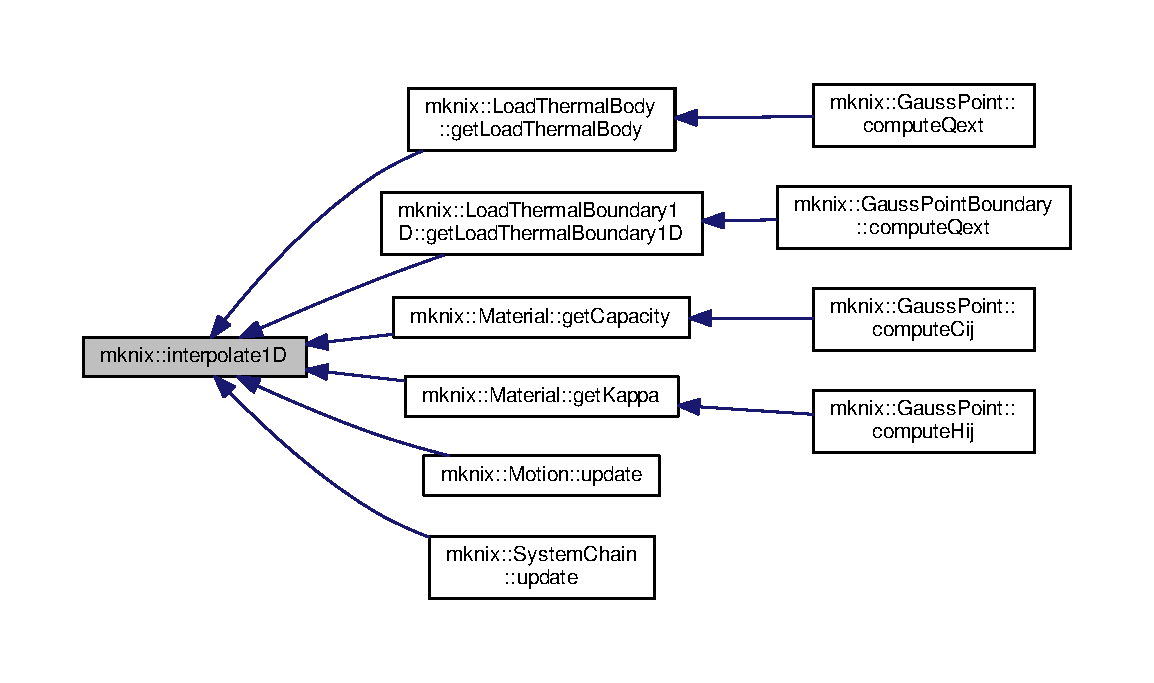
\includegraphics[width=350pt]{d2/dde/namespacemknix_a3c53b5663b9039ec67691eea93bb7f54_icgraph}
\end{center}
\end{figure}


\hypertarget{namespacemknix_a7635c8b68c992d53466bf5083e9c7ae2}{}\index{mknix@{mknix}!make\+\_\+unique@{make\+\_\+unique}}
\index{make\+\_\+unique@{make\+\_\+unique}!mknix@{mknix}}
\paragraph[{make\+\_\+unique}]{\setlength{\rightskip}{0pt plus 5cm}template$<$class T , class... Args$>$ std\+::unique\+\_\+ptr$<$T$>$ mknix\+::make\+\_\+unique (
\begin{DoxyParamCaption}
\item[{Args \&\&...}]{args}
\end{DoxyParamCaption}
)}\label{namespacemknix_a7635c8b68c992d53466bf5083e9c7ae2}
Stand-\/in for std\+::make\+\_\+unique included in C++14 

Definition at line 36 of file common.\+h.

\hypertarget{namespacemknix_a8f5fd36c13ae99d02e930a9dad382721}{}\index{mknix@{mknix}!set\+Signal@{set\+Signal}}
\index{set\+Signal@{set\+Signal}!mknix@{mknix}}
\paragraph[{set\+Signal}]{\setlength{\rightskip}{0pt plus 5cm}void mknix\+::set\+Signal (
\begin{DoxyParamCaption}
\item[{std\+::string}]{node, }
\item[{std\+::vector$<$ double $>$}]{}
\end{DoxyParamCaption}
)}\label{namespacemknix_a8f5fd36c13ae99d02e930a9dad382721}


Definition at line 202 of file simulation.\+cpp.


\section{Class Documentation}
\hypertarget{classmknix_1_1_analysis}{\subsection{mknix\-:\-:Analysis Class Reference}
\label{classmknix_1_1_analysis}\index{mknix\-::\-Analysis@{mknix\-::\-Analysis}}
}


{\ttfamily \#include $<$analysis.\-h$>$}



Inheritance diagram for mknix\-:\-:Analysis\-:\nopagebreak
\begin{figure}[H]
\begin{center}
\leavevmode
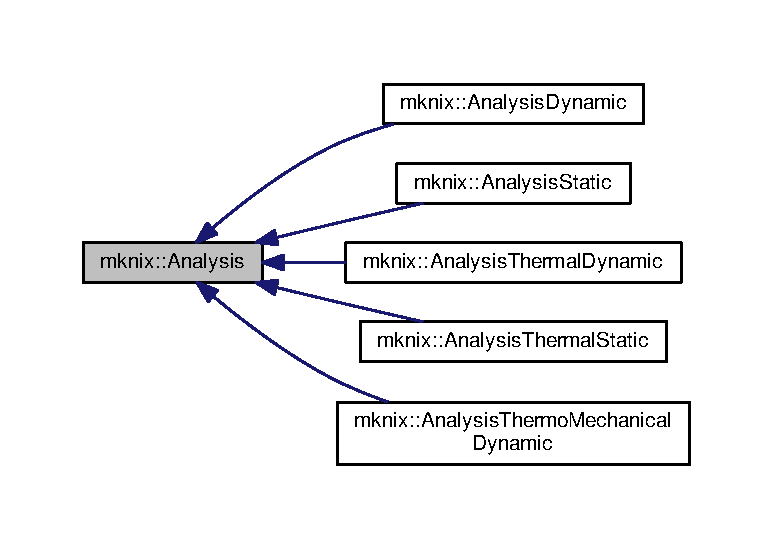
\includegraphics[width=350pt]{dc/d6f/classmknix_1_1_analysis__inherit__graph}
\end{center}
\end{figure}


Collaboration diagram for mknix\-:\-:Analysis\-:\nopagebreak
\begin{figure}[H]
\begin{center}
\leavevmode
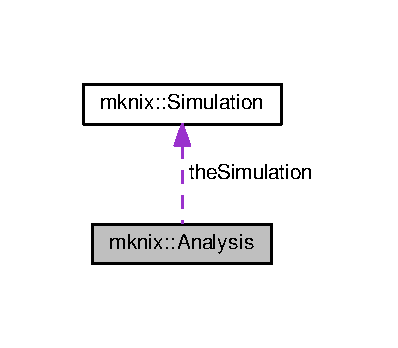
\includegraphics[width=190pt]{d5/d73/classmknix_1_1_analysis__coll__graph}
\end{center}
\end{figure}
\subsubsection*{Public Member Functions}
\begin{DoxyCompactItemize}
\item 
\hyperlink{classmknix_1_1_analysis_a524d9cd12f302975c64a0c4266cd91ed}{Analysis} ()
\item 
\hyperlink{classmknix_1_1_analysis_a58f5b79c2b28457ae18186991306abb3}{Analysis} (\hyperlink{classmknix_1_1_simulation}{Simulation} $\ast$)
\item 
virtual \hyperlink{classmknix_1_1_analysis_a4813618a04dd0c3098a58b60792f2e34}{$\sim$\-Analysis} ()
\item 
virtual std\-::string \hyperlink{classmknix_1_1_analysis_a6dd7026a22ae11f3eef3dad3be370e70}{type} ()=0
\item 
void \hyperlink{classmknix_1_1_analysis_a4e6baab7f63725b4ed816bb3bdbdc1d8}{set\-Epsilon} (double epsilon\-\_\-in)
\item 
virtual void \hyperlink{classmknix_1_1_analysis_a2a02ee6ab0728bc1ab5e6aab010afe87}{solve} (lmx\-::\-Vector$<$ \hyperlink{namespacemknix_a16be4b246fbf2cceb141e3a179111020}{data\-\_\-type} $>$ $\ast$, lmx\-::\-Vector$<$ \hyperlink{namespacemknix_a16be4b246fbf2cceb141e3a179111020}{data\-\_\-type} $>$ $\ast$=0)=0
\end{DoxyCompactItemize}
\subsubsection*{Protected Attributes}
\begin{DoxyCompactItemize}
\item 
\hyperlink{classmknix_1_1_simulation}{Simulation} $\ast$ \hyperlink{classmknix_1_1_analysis_a1abc29e3b8565590b6bf0ce2d8b3b68f}{the\-Simulation}
\item 
double \hyperlink{classmknix_1_1_analysis_a7e0439caf5fa5f90d808acec6d75b72f}{epsilon}
\end{DoxyCompactItemize}


\subsubsection{Detailed Description}
\begin{DoxyAuthor}{Author}
A\-U\-T\-H\-O\-R\-S $<$\-M\-A\-I\-L\-S$>$ 
\end{DoxyAuthor}


\subsubsection{Constructor \& Destructor Documentation}
\hypertarget{classmknix_1_1_analysis_a524d9cd12f302975c64a0c4266cd91ed}{\index{mknix\-::\-Analysis@{mknix\-::\-Analysis}!Analysis@{Analysis}}
\index{Analysis@{Analysis}!mknix::Analysis@{mknix\-::\-Analysis}}
\paragraph[{Analysis}]{\setlength{\rightskip}{0pt plus 5cm}mknix\-::\-Analysis\-::\-Analysis (
\begin{DoxyParamCaption}
{}
\end{DoxyParamCaption}
)}}\label{classmknix_1_1_analysis_a524d9cd12f302975c64a0c4266cd91ed}
\hypertarget{classmknix_1_1_analysis_a58f5b79c2b28457ae18186991306abb3}{\index{mknix\-::\-Analysis@{mknix\-::\-Analysis}!Analysis@{Analysis}}
\index{Analysis@{Analysis}!mknix::Analysis@{mknix\-::\-Analysis}}
\paragraph[{Analysis}]{\setlength{\rightskip}{0pt plus 5cm}mknix\-::\-Analysis\-::\-Analysis (
\begin{DoxyParamCaption}
\item[{{\bf Simulation} $\ast$}]{simulation\-\_\-in}
\end{DoxyParamCaption}
)}}\label{classmknix_1_1_analysis_a58f5b79c2b28457ae18186991306abb3}
\hypertarget{classmknix_1_1_analysis_a4813618a04dd0c3098a58b60792f2e34}{\index{mknix\-::\-Analysis@{mknix\-::\-Analysis}!$\sim$\-Analysis@{$\sim$\-Analysis}}
\index{$\sim$\-Analysis@{$\sim$\-Analysis}!mknix::Analysis@{mknix\-::\-Analysis}}
\paragraph[{$\sim$\-Analysis}]{\setlength{\rightskip}{0pt plus 5cm}mknix\-::\-Analysis\-::$\sim$\-Analysis (
\begin{DoxyParamCaption}
{}
\end{DoxyParamCaption}
)\hspace{0.3cm}{\ttfamily [virtual]}}}\label{classmknix_1_1_analysis_a4813618a04dd0c3098a58b60792f2e34}


\subsubsection{Member Function Documentation}
\hypertarget{classmknix_1_1_analysis_a4e6baab7f63725b4ed816bb3bdbdc1d8}{\index{mknix\-::\-Analysis@{mknix\-::\-Analysis}!set\-Epsilon@{set\-Epsilon}}
\index{set\-Epsilon@{set\-Epsilon}!mknix::Analysis@{mknix\-::\-Analysis}}
\paragraph[{set\-Epsilon}]{\setlength{\rightskip}{0pt plus 5cm}void mknix\-::\-Analysis\-::set\-Epsilon (
\begin{DoxyParamCaption}
\item[{double}]{epsilon\-\_\-in}
\end{DoxyParamCaption}
)\hspace{0.3cm}{\ttfamily [inline]}}}\label{classmknix_1_1_analysis_a4e6baab7f63725b4ed816bb3bdbdc1d8}


Here is the caller graph for this function\-:\nopagebreak
\begin{figure}[H]
\begin{center}
\leavevmode
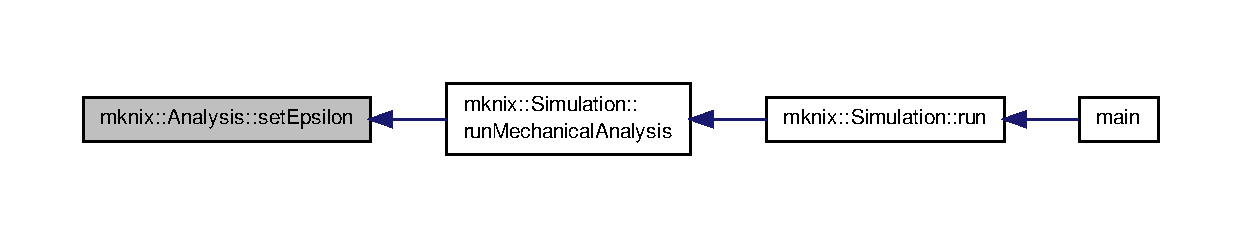
\includegraphics[width=350pt]{df/d86/classmknix_1_1_analysis_a4e6baab7f63725b4ed816bb3bdbdc1d8_icgraph}
\end{center}
\end{figure}


\hypertarget{classmknix_1_1_analysis_a2a02ee6ab0728bc1ab5e6aab010afe87}{\index{mknix\-::\-Analysis@{mknix\-::\-Analysis}!solve@{solve}}
\index{solve@{solve}!mknix::Analysis@{mknix\-::\-Analysis}}
\paragraph[{solve}]{\setlength{\rightskip}{0pt plus 5cm}virtual void mknix\-::\-Analysis\-::solve (
\begin{DoxyParamCaption}
\item[{lmx\-::\-Vector$<$ {\bf data\-\_\-type} $>$ $\ast$}]{, }
\item[{lmx\-::\-Vector$<$ {\bf data\-\_\-type} $>$ $\ast$}]{ = {\ttfamily 0}}
\end{DoxyParamCaption}
)\hspace{0.3cm}{\ttfamily [pure virtual]}}}\label{classmknix_1_1_analysis_a2a02ee6ab0728bc1ab5e6aab010afe87}


Implemented in \hyperlink{classmknix_1_1_analysis_dynamic_a43c9ab1907cb3cd72f3f4d605d2fa8ae}{mknix\-::\-Analysis\-Dynamic}, \hyperlink{classmknix_1_1_analysis_static_a1f2d048b8625d58f820a7f7d8dfe2f7d}{mknix\-::\-Analysis\-Static}, \hyperlink{classmknix_1_1_analysis_thermal_dynamic_aafe2cdc0b12567535eedc9f675c0944d}{mknix\-::\-Analysis\-Thermal\-Dynamic}, and \hyperlink{classmknix_1_1_analysis_thermal_static_a603b8f8431172ab62f351393cb60adae}{mknix\-::\-Analysis\-Thermal\-Static}.



Here is the caller graph for this function\-:\nopagebreak
\begin{figure}[H]
\begin{center}
\leavevmode
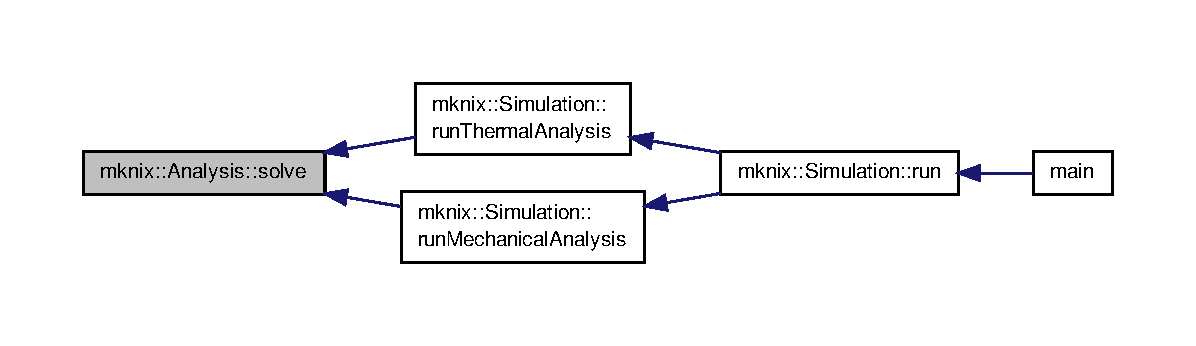
\includegraphics[width=350pt]{df/d86/classmknix_1_1_analysis_a2a02ee6ab0728bc1ab5e6aab010afe87_icgraph}
\end{center}
\end{figure}


\hypertarget{classmknix_1_1_analysis_a6dd7026a22ae11f3eef3dad3be370e70}{\index{mknix\-::\-Analysis@{mknix\-::\-Analysis}!type@{type}}
\index{type@{type}!mknix::Analysis@{mknix\-::\-Analysis}}
\paragraph[{type}]{\setlength{\rightskip}{0pt plus 5cm}virtual std\-::string mknix\-::\-Analysis\-::type (
\begin{DoxyParamCaption}
{}
\end{DoxyParamCaption}
)\hspace{0.3cm}{\ttfamily [pure virtual]}}}\label{classmknix_1_1_analysis_a6dd7026a22ae11f3eef3dad3be370e70}


Implemented in \hyperlink{classmknix_1_1_analysis_dynamic_a10045ff80be02d24dc08ad7da248844f}{mknix\-::\-Analysis\-Dynamic}, \hyperlink{classmknix_1_1_analysis_static_a14ab31bf7d144b576cbc7ea8de0d4fd9}{mknix\-::\-Analysis\-Static}, \hyperlink{classmknix_1_1_analysis_thermal_dynamic_ae1d271bfca189706a101259cff192ec9}{mknix\-::\-Analysis\-Thermal\-Dynamic}, and \hyperlink{classmknix_1_1_analysis_thermal_static_a14a7b53403f7523ccb783129e928241b}{mknix\-::\-Analysis\-Thermal\-Static}.



Here is the caller graph for this function\-:\nopagebreak
\begin{figure}[H]
\begin{center}
\leavevmode
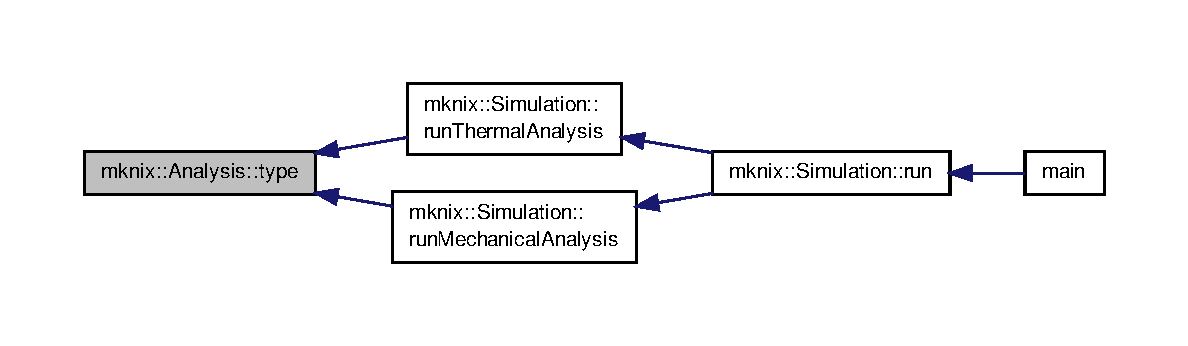
\includegraphics[width=350pt]{df/d86/classmknix_1_1_analysis_a6dd7026a22ae11f3eef3dad3be370e70_icgraph}
\end{center}
\end{figure}




\subsubsection{Member Data Documentation}
\hypertarget{classmknix_1_1_analysis_a7e0439caf5fa5f90d808acec6d75b72f}{\index{mknix\-::\-Analysis@{mknix\-::\-Analysis}!epsilon@{epsilon}}
\index{epsilon@{epsilon}!mknix::Analysis@{mknix\-::\-Analysis}}
\paragraph[{epsilon}]{\setlength{\rightskip}{0pt plus 5cm}double mknix\-::\-Analysis\-::epsilon\hspace{0.3cm}{\ttfamily [protected]}}}\label{classmknix_1_1_analysis_a7e0439caf5fa5f90d808acec6d75b72f}
\hypertarget{classmknix_1_1_analysis_a1abc29e3b8565590b6bf0ce2d8b3b68f}{\index{mknix\-::\-Analysis@{mknix\-::\-Analysis}!the\-Simulation@{the\-Simulation}}
\index{the\-Simulation@{the\-Simulation}!mknix::Analysis@{mknix\-::\-Analysis}}
\paragraph[{the\-Simulation}]{\setlength{\rightskip}{0pt plus 5cm}{\bf Simulation}$\ast$ mknix\-::\-Analysis\-::the\-Simulation\hspace{0.3cm}{\ttfamily [protected]}}}\label{classmknix_1_1_analysis_a1abc29e3b8565590b6bf0ce2d8b3b68f}


The documentation for this class was generated from the following files\-:\begin{DoxyCompactItemize}
\item 
\hyperlink{analysis_8h}{analysis.\-h}\item 
\hyperlink{analysis_8cpp}{analysis.\-cpp}\end{DoxyCompactItemize}

\hypertarget{classmknix_1_1_analysis_dynamic}{\subsection{mknix\-:\-:Analysis\-Dynamic Class Reference}
\label{classmknix_1_1_analysis_dynamic}\index{mknix\-::\-Analysis\-Dynamic@{mknix\-::\-Analysis\-Dynamic}}
}


{\ttfamily \#include $<$analysisdynamic.\-h$>$}



Inheritance diagram for mknix\-:\-:Analysis\-Dynamic\-:\nopagebreak
\begin{figure}[H]
\begin{center}
\leavevmode
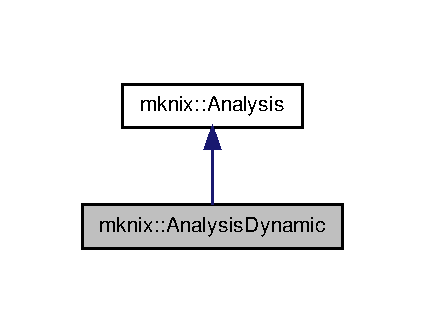
\includegraphics[width=204pt]{da/dfd/classmknix_1_1_analysis_dynamic__inherit__graph}
\end{center}
\end{figure}


Collaboration diagram for mknix\-:\-:Analysis\-Dynamic\-:\nopagebreak
\begin{figure}[H]
\begin{center}
\leavevmode
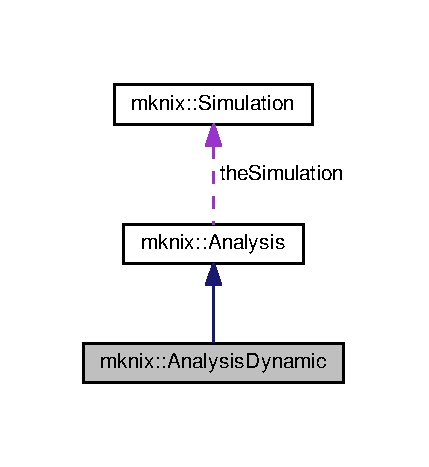
\includegraphics[width=205pt]{d7/d8a/classmknix_1_1_analysis_dynamic__coll__graph}
\end{center}
\end{figure}
\subsubsection*{Public Member Functions}
\begin{DoxyCompactItemize}
\item 
\hyperlink{classmknix_1_1_analysis_dynamic_a1457ddff8dfa14a90605248f4b953851}{Analysis\-Dynamic} ()
\item 
\hyperlink{classmknix_1_1_analysis_dynamic_a452203e81d27283089fe500b32c7ab55}{Analysis\-Dynamic} (\hyperlink{classmknix_1_1_simulation}{Simulation} $\ast$, double, double, double, char $\ast$, double, double, double)
\item 
\hyperlink{classmknix_1_1_analysis_dynamic_a85fd7662ea3228c608c6761ffc4e46d4}{$\sim$\-Analysis\-Dynamic} ()
\item 
std\-::string \hyperlink{classmknix_1_1_analysis_dynamic_a10045ff80be02d24dc08ad7da248844f}{type} ()
\item 
void \hyperlink{classmknix_1_1_analysis_dynamic_a43c9ab1907cb3cd72f3f4d605d2fa8ae}{solve} (lmx\-::\-Vector$<$ \hyperlink{namespacemknix_a16be4b246fbf2cceb141e3a179111020}{data\-\_\-type} $>$ $\ast$, lmx\-::\-Vector$<$ \hyperlink{namespacemknix_a16be4b246fbf2cceb141e3a179111020}{data\-\_\-type} $>$ $\ast$)
\end{DoxyCompactItemize}
\subsubsection*{Additional Inherited Members}


\subsubsection{Detailed Description}
\begin{DoxyAuthor}{Author}
A\-U\-T\-H\-O\-R\-S $<$\-M\-A\-I\-L\-S$>$ 
\end{DoxyAuthor}


\subsubsection{Constructor \& Destructor Documentation}
\hypertarget{classmknix_1_1_analysis_dynamic_a1457ddff8dfa14a90605248f4b953851}{\index{mknix\-::\-Analysis\-Dynamic@{mknix\-::\-Analysis\-Dynamic}!Analysis\-Dynamic@{Analysis\-Dynamic}}
\index{Analysis\-Dynamic@{Analysis\-Dynamic}!mknix::AnalysisDynamic@{mknix\-::\-Analysis\-Dynamic}}
\paragraph[{Analysis\-Dynamic}]{\setlength{\rightskip}{0pt plus 5cm}mknix\-::\-Analysis\-Dynamic\-::\-Analysis\-Dynamic (
\begin{DoxyParamCaption}
{}
\end{DoxyParamCaption}
)}}\label{classmknix_1_1_analysis_dynamic_a1457ddff8dfa14a90605248f4b953851}
\hypertarget{classmknix_1_1_analysis_dynamic_a452203e81d27283089fe500b32c7ab55}{\index{mknix\-::\-Analysis\-Dynamic@{mknix\-::\-Analysis\-Dynamic}!Analysis\-Dynamic@{Analysis\-Dynamic}}
\index{Analysis\-Dynamic@{Analysis\-Dynamic}!mknix::AnalysisDynamic@{mknix\-::\-Analysis\-Dynamic}}
\paragraph[{Analysis\-Dynamic}]{\setlength{\rightskip}{0pt plus 5cm}mknix\-::\-Analysis\-Dynamic\-::\-Analysis\-Dynamic (
\begin{DoxyParamCaption}
\item[{{\bf Simulation} $\ast$}]{simulation\-\_\-in, }
\item[{double}]{to\-\_\-in, }
\item[{double}]{tf\-\_\-in, }
\item[{double}]{At\-\_\-in, }
\item[{char $\ast$}]{integrator\-\_\-in, }
\item[{double}]{par1 = {\ttfamily -\/1.}, }
\item[{double}]{par2 = {\ttfamily -\/1.}, }
\item[{double}]{par3 = {\ttfamily -\/1.}}
\end{DoxyParamCaption}
)}}\label{classmknix_1_1_analysis_dynamic_a452203e81d27283089fe500b32c7ab55}


Here is the call graph for this function\-:\nopagebreak
\begin{figure}[H]
\begin{center}
\leavevmode
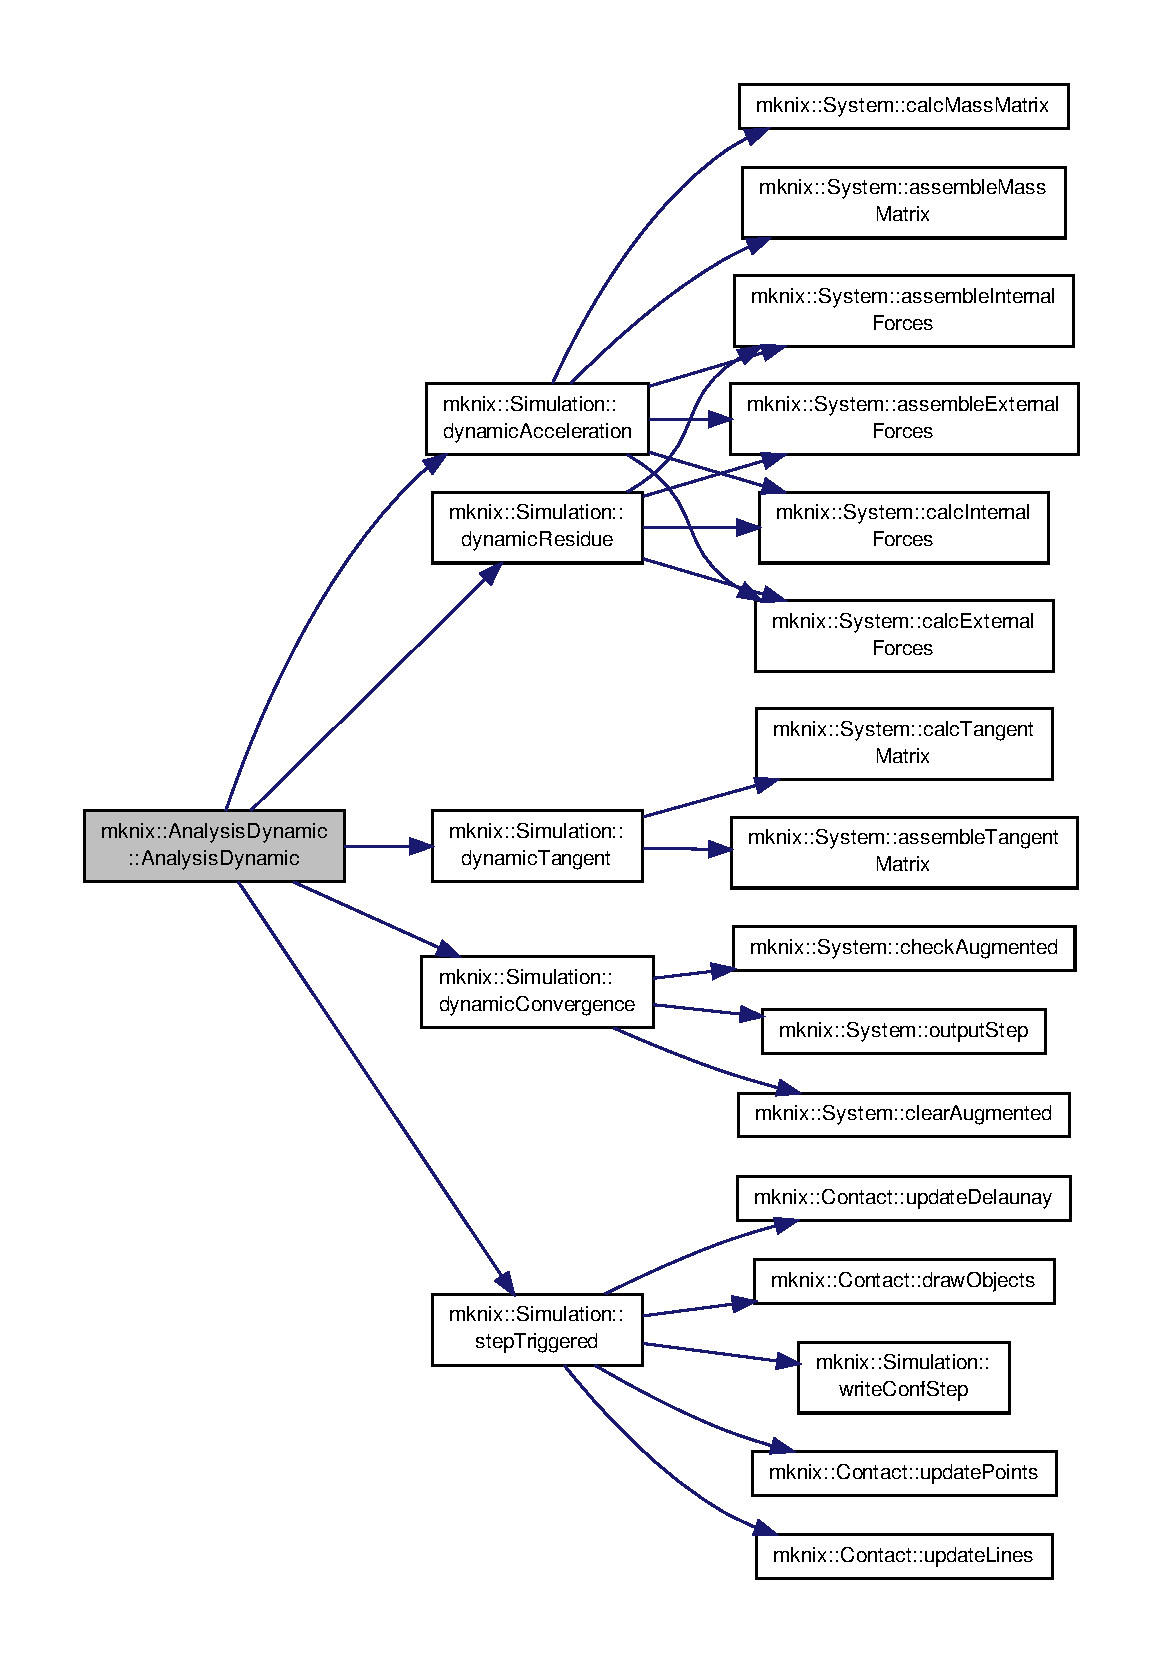
\includegraphics[width=350pt]{d4/d8c/classmknix_1_1_analysis_dynamic_a452203e81d27283089fe500b32c7ab55_cgraph}
\end{center}
\end{figure}


\hypertarget{classmknix_1_1_analysis_dynamic_a85fd7662ea3228c608c6761ffc4e46d4}{\index{mknix\-::\-Analysis\-Dynamic@{mknix\-::\-Analysis\-Dynamic}!$\sim$\-Analysis\-Dynamic@{$\sim$\-Analysis\-Dynamic}}
\index{$\sim$\-Analysis\-Dynamic@{$\sim$\-Analysis\-Dynamic}!mknix::AnalysisDynamic@{mknix\-::\-Analysis\-Dynamic}}
\paragraph[{$\sim$\-Analysis\-Dynamic}]{\setlength{\rightskip}{0pt plus 5cm}mknix\-::\-Analysis\-Dynamic\-::$\sim$\-Analysis\-Dynamic (
\begin{DoxyParamCaption}
{}
\end{DoxyParamCaption}
)}}\label{classmknix_1_1_analysis_dynamic_a85fd7662ea3228c608c6761ffc4e46d4}


\subsubsection{Member Function Documentation}
\hypertarget{classmknix_1_1_analysis_dynamic_a43c9ab1907cb3cd72f3f4d605d2fa8ae}{\index{mknix\-::\-Analysis\-Dynamic@{mknix\-::\-Analysis\-Dynamic}!solve@{solve}}
\index{solve@{solve}!mknix::AnalysisDynamic@{mknix\-::\-Analysis\-Dynamic}}
\paragraph[{solve}]{\setlength{\rightskip}{0pt plus 5cm}void mknix\-::\-Analysis\-Dynamic\-::solve (
\begin{DoxyParamCaption}
\item[{lmx\-::\-Vector$<$ {\bf data\-\_\-type} $>$ $\ast$}]{q\-\_\-in, }
\item[{lmx\-::\-Vector$<$ {\bf data\-\_\-type} $>$ $\ast$}]{qdot\-\_\-in}
\end{DoxyParamCaption}
)\hspace{0.3cm}{\ttfamily [virtual]}}}\label{classmknix_1_1_analysis_dynamic_a43c9ab1907cb3cd72f3f4d605d2fa8ae}


Implements \hyperlink{classmknix_1_1_analysis_a2a02ee6ab0728bc1ab5e6aab010afe87}{mknix\-::\-Analysis}.



Here is the call graph for this function\-:\nopagebreak
\begin{figure}[H]
\begin{center}
\leavevmode
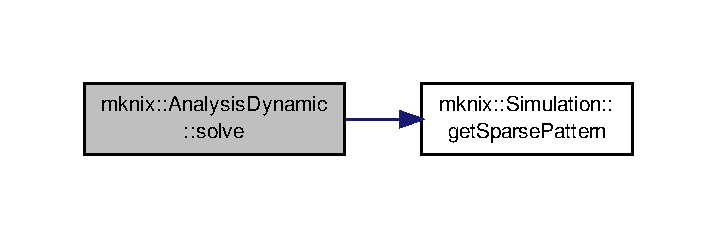
\includegraphics[width=344pt]{d4/d8c/classmknix_1_1_analysis_dynamic_a43c9ab1907cb3cd72f3f4d605d2fa8ae_cgraph}
\end{center}
\end{figure}


\hypertarget{classmknix_1_1_analysis_dynamic_a10045ff80be02d24dc08ad7da248844f}{\index{mknix\-::\-Analysis\-Dynamic@{mknix\-::\-Analysis\-Dynamic}!type@{type}}
\index{type@{type}!mknix::AnalysisDynamic@{mknix\-::\-Analysis\-Dynamic}}
\paragraph[{type}]{\setlength{\rightskip}{0pt plus 5cm}std\-::string mknix\-::\-Analysis\-Dynamic\-::type (
\begin{DoxyParamCaption}
{}
\end{DoxyParamCaption}
)\hspace{0.3cm}{\ttfamily [inline]}, {\ttfamily [virtual]}}}\label{classmknix_1_1_analysis_dynamic_a10045ff80be02d24dc08ad7da248844f}


Implements \hyperlink{classmknix_1_1_analysis_a6dd7026a22ae11f3eef3dad3be370e70}{mknix\-::\-Analysis}.



The documentation for this class was generated from the following files\-:\begin{DoxyCompactItemize}
\item 
\hyperlink{analysisdynamic_8h}{analysisdynamic.\-h}\item 
\hyperlink{analysisdynamic_8cpp}{analysisdynamic.\-cpp}\end{DoxyCompactItemize}

\hypertarget{classmknix_1_1_analysis_static}{\subsection{mknix\-:\-:Analysis\-Static Class Reference}
\label{classmknix_1_1_analysis_static}\index{mknix\-::\-Analysis\-Static@{mknix\-::\-Analysis\-Static}}
}


{\ttfamily \#include $<$analysisstatic.\-h$>$}



Inheritance diagram for mknix\-:\-:Analysis\-Static\-:\nopagebreak
\begin{figure}[H]
\begin{center}
\leavevmode
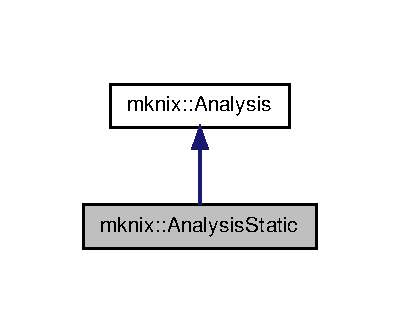
\includegraphics[width=192pt]{dd/dc4/classmknix_1_1_analysis_static__inherit__graph}
\end{center}
\end{figure}


Collaboration diagram for mknix\-:\-:Analysis\-Static\-:\nopagebreak
\begin{figure}[H]
\begin{center}
\leavevmode
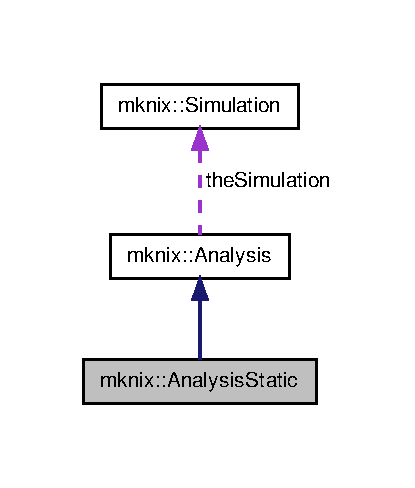
\includegraphics[width=199pt]{d2/dab/classmknix_1_1_analysis_static__coll__graph}
\end{center}
\end{figure}
\subsubsection*{Public Member Functions}
\begin{DoxyCompactItemize}
\item 
\hyperlink{classmknix_1_1_analysis_static_ac64781280792830016fe43f344966f99}{Analysis\-Static} ()
\item 
\hyperlink{classmknix_1_1_analysis_static_a18cfe64c3b4b6b3f54acc3caa6780e92}{Analysis\-Static} (\hyperlink{classmknix_1_1_simulation}{Simulation} $\ast$, double)
\item 
\hyperlink{classmknix_1_1_analysis_static_a67877fe7b967f91b1b8c92cf4afe1658}{$\sim$\-Analysis\-Static} ()
\item 
std\-::string \hyperlink{classmknix_1_1_analysis_static_a14ab31bf7d144b576cbc7ea8de0d4fd9}{type} ()
\item 
void \hyperlink{classmknix_1_1_analysis_static_a1f2d048b8625d58f820a7f7d8dfe2f7d}{solve} (lmx\-::\-Vector$<$ \hyperlink{namespacemknix_a16be4b246fbf2cceb141e3a179111020}{data\-\_\-type} $>$ $\ast$, lmx\-::\-Vector$<$ \hyperlink{namespacemknix_a16be4b246fbf2cceb141e3a179111020}{data\-\_\-type} $>$ $\ast$)
\end{DoxyCompactItemize}
\subsubsection*{Additional Inherited Members}


\subsubsection{Detailed Description}
\begin{DoxyAuthor}{Author}
A\-U\-T\-H\-O\-R\-S $<$\-M\-A\-I\-L\-S$>$ 
\end{DoxyAuthor}


\subsubsection{Constructor \& Destructor Documentation}
\hypertarget{classmknix_1_1_analysis_static_ac64781280792830016fe43f344966f99}{\index{mknix\-::\-Analysis\-Static@{mknix\-::\-Analysis\-Static}!Analysis\-Static@{Analysis\-Static}}
\index{Analysis\-Static@{Analysis\-Static}!mknix::AnalysisStatic@{mknix\-::\-Analysis\-Static}}
\paragraph[{Analysis\-Static}]{\setlength{\rightskip}{0pt plus 5cm}mknix\-::\-Analysis\-Static\-::\-Analysis\-Static (
\begin{DoxyParamCaption}
{}
\end{DoxyParamCaption}
)}}\label{classmknix_1_1_analysis_static_ac64781280792830016fe43f344966f99}
\hypertarget{classmknix_1_1_analysis_static_a18cfe64c3b4b6b3f54acc3caa6780e92}{\index{mknix\-::\-Analysis\-Static@{mknix\-::\-Analysis\-Static}!Analysis\-Static@{Analysis\-Static}}
\index{Analysis\-Static@{Analysis\-Static}!mknix::AnalysisStatic@{mknix\-::\-Analysis\-Static}}
\paragraph[{Analysis\-Static}]{\setlength{\rightskip}{0pt plus 5cm}mknix\-::\-Analysis\-Static\-::\-Analysis\-Static (
\begin{DoxyParamCaption}
\item[{{\bf Simulation} $\ast$}]{simulation\-\_\-in, }
\item[{double}]{time\-\_\-in}
\end{DoxyParamCaption}
)}}\label{classmknix_1_1_analysis_static_a18cfe64c3b4b6b3f54acc3caa6780e92}


Here is the call graph for this function\-:\nopagebreak
\begin{figure}[H]
\begin{center}
\leavevmode
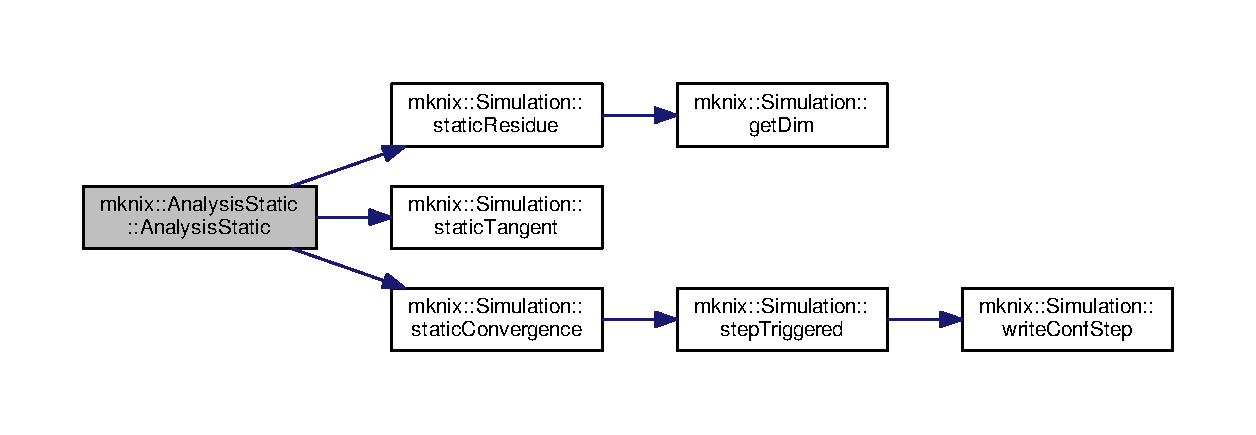
\includegraphics[width=350pt]{db/d8f/classmknix_1_1_analysis_static_a18cfe64c3b4b6b3f54acc3caa6780e92_cgraph}
\end{center}
\end{figure}


\hypertarget{classmknix_1_1_analysis_static_a67877fe7b967f91b1b8c92cf4afe1658}{\index{mknix\-::\-Analysis\-Static@{mknix\-::\-Analysis\-Static}!$\sim$\-Analysis\-Static@{$\sim$\-Analysis\-Static}}
\index{$\sim$\-Analysis\-Static@{$\sim$\-Analysis\-Static}!mknix::AnalysisStatic@{mknix\-::\-Analysis\-Static}}
\paragraph[{$\sim$\-Analysis\-Static}]{\setlength{\rightskip}{0pt plus 5cm}mknix\-::\-Analysis\-Static\-::$\sim$\-Analysis\-Static (
\begin{DoxyParamCaption}
{}
\end{DoxyParamCaption}
)}}\label{classmknix_1_1_analysis_static_a67877fe7b967f91b1b8c92cf4afe1658}


\subsubsection{Member Function Documentation}
\hypertarget{classmknix_1_1_analysis_static_a1f2d048b8625d58f820a7f7d8dfe2f7d}{\index{mknix\-::\-Analysis\-Static@{mknix\-::\-Analysis\-Static}!solve@{solve}}
\index{solve@{solve}!mknix::AnalysisStatic@{mknix\-::\-Analysis\-Static}}
\paragraph[{solve}]{\setlength{\rightskip}{0pt plus 5cm}void mknix\-::\-Analysis\-Static\-::solve (
\begin{DoxyParamCaption}
\item[{lmx\-::\-Vector$<$ {\bf data\-\_\-type} $>$ $\ast$}]{q\-\_\-in, }
\item[{lmx\-::\-Vector$<$ {\bf data\-\_\-type} $>$ $\ast$}]{qdot\-\_\-in = {\ttfamily 0}}
\end{DoxyParamCaption}
)\hspace{0.3cm}{\ttfamily [virtual]}}}\label{classmknix_1_1_analysis_static_a1f2d048b8625d58f820a7f7d8dfe2f7d}


Implements \hyperlink{classmknix_1_1_analysis_a2a02ee6ab0728bc1ab5e6aab010afe87}{mknix\-::\-Analysis}.

\hypertarget{classmknix_1_1_analysis_static_a14ab31bf7d144b576cbc7ea8de0d4fd9}{\index{mknix\-::\-Analysis\-Static@{mknix\-::\-Analysis\-Static}!type@{type}}
\index{type@{type}!mknix::AnalysisStatic@{mknix\-::\-Analysis\-Static}}
\paragraph[{type}]{\setlength{\rightskip}{0pt plus 5cm}std\-::string mknix\-::\-Analysis\-Static\-::type (
\begin{DoxyParamCaption}
{}
\end{DoxyParamCaption}
)\hspace{0.3cm}{\ttfamily [inline]}, {\ttfamily [virtual]}}}\label{classmknix_1_1_analysis_static_a14ab31bf7d144b576cbc7ea8de0d4fd9}


Implements \hyperlink{classmknix_1_1_analysis_a6dd7026a22ae11f3eef3dad3be370e70}{mknix\-::\-Analysis}.



The documentation for this class was generated from the following files\-:\begin{DoxyCompactItemize}
\item 
\hyperlink{analysisstatic_8h}{analysisstatic.\-h}\item 
\hyperlink{analysisstatic_8cpp}{analysisstatic.\-cpp}\end{DoxyCompactItemize}

\hypertarget{classmknix_1_1_analysis_thermal_dynamic}{}\subsection{mknix\+:\+:Analysis\+Thermal\+Dynamic Class Reference}
\label{classmknix_1_1_analysis_thermal_dynamic}\index{mknix\+::\+Analysis\+Thermal\+Dynamic@{mknix\+::\+Analysis\+Thermal\+Dynamic}}


{\ttfamily \#include $<$analysisthermaldynamic.\+h$>$}



Inheritance diagram for mknix\+:\+:Analysis\+Thermal\+Dynamic\+:\nopagebreak
\begin{figure}[H]
\begin{center}
\leavevmode
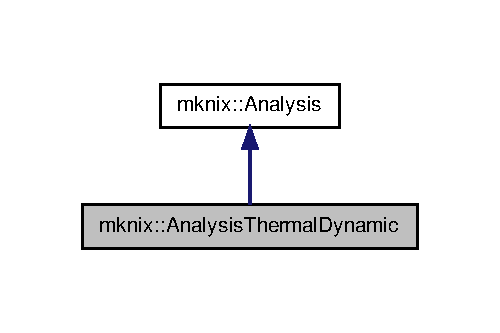
\includegraphics[width=241pt]{df/da8/classmknix_1_1_analysis_thermal_dynamic__inherit__graph}
\end{center}
\end{figure}


Collaboration diagram for mknix\+:\+:Analysis\+Thermal\+Dynamic\+:\nopagebreak
\begin{figure}[H]
\begin{center}
\leavevmode
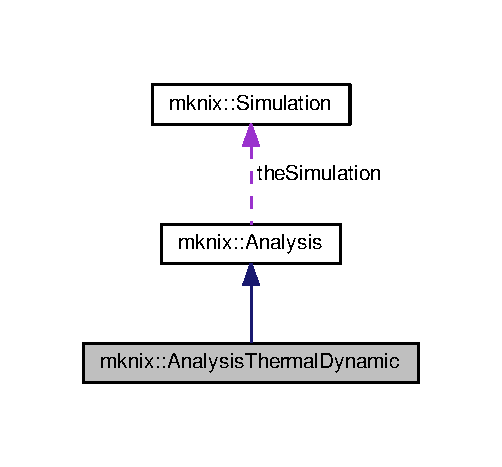
\includegraphics[width=241pt]{db/d46/classmknix_1_1_analysis_thermal_dynamic__coll__graph}
\end{center}
\end{figure}
\subsubsection*{Public Member Functions}
\begin{DoxyCompactItemize}
\item 
\hyperlink{classmknix_1_1_analysis_thermal_dynamic_a475e28b3bb7b7a9d2cf3628863bd8291}{Analysis\+Thermal\+Dynamic} ()
\item 
\hyperlink{classmknix_1_1_analysis_thermal_dynamic_a161ebe1ed696232ed05ef778cdcabcb8}{Analysis\+Thermal\+Dynamic} (\hyperlink{classmknix_1_1_simulation}{Simulation} $\ast$, double, double, double, char $\ast$)
\item 
\hyperlink{classmknix_1_1_analysis_thermal_dynamic_ad0dbaa6affc6e4a285d310e209fe2b73}{$\sim$\+Analysis\+Thermal\+Dynamic} ()
\item 
std\+::string \hyperlink{classmknix_1_1_analysis_thermal_dynamic_ae1d271bfca189706a101259cff192ec9}{type} ()
\item 
void \hyperlink{classmknix_1_1_analysis_thermal_dynamic_a616aac65d4489996979a0c9120089e37}{init} (\hyperlink{classlmx_1_1_vector}{lmx\+::\+Vector}$<$ \hyperlink{namespacemknix_a16be4b246fbf2cceb141e3a179111020}{data\+\_\+type} $>$ $\ast$)
\item 
void \hyperlink{classmknix_1_1_analysis_thermal_dynamic_a2c5b1abfa4cfbfea523e27286146fe77}{next\+Step} ()
\item 
void \hyperlink{classmknix_1_1_analysis_thermal_dynamic_a17a9d48a88a1268960dc15371ab703a7}{solve} (\hyperlink{classlmx_1_1_vector}{lmx\+::\+Vector}$<$ \hyperlink{namespacemknix_a16be4b246fbf2cceb141e3a179111020}{data\+\_\+type} $>$ $\ast$, \hyperlink{classlmx_1_1_vector}{lmx\+::\+Vector}$<$ \hyperlink{namespacemknix_a16be4b246fbf2cceb141e3a179111020}{data\+\_\+type} $>$ $\ast$, \hyperlink{classlmx_1_1_vector}{lmx\+::\+Vector}$<$ \hyperlink{namespacemknix_a16be4b246fbf2cceb141e3a179111020}{data\+\_\+type} $>$ $\ast$)
\end{DoxyCompactItemize}
\subsubsection*{Additional Inherited Members}


\subsubsection{Detailed Description}
\begin{DoxyAuthor}{Author}
A\+U\+T\+H\+O\+R\+S $<$\+M\+A\+I\+L\+S$>$ 
\end{DoxyAuthor}


Definition at line 30 of file analysisthermaldynamic.\+h.



\subsubsection{Constructor \& Destructor Documentation}
\hypertarget{classmknix_1_1_analysis_thermal_dynamic_a475e28b3bb7b7a9d2cf3628863bd8291}{}\index{mknix\+::\+Analysis\+Thermal\+Dynamic@{mknix\+::\+Analysis\+Thermal\+Dynamic}!Analysis\+Thermal\+Dynamic@{Analysis\+Thermal\+Dynamic}}
\index{Analysis\+Thermal\+Dynamic@{Analysis\+Thermal\+Dynamic}!mknix\+::\+Analysis\+Thermal\+Dynamic@{mknix\+::\+Analysis\+Thermal\+Dynamic}}
\paragraph[{Analysis\+Thermal\+Dynamic}]{\setlength{\rightskip}{0pt plus 5cm}mknix\+::\+Analysis\+Thermal\+Dynamic\+::\+Analysis\+Thermal\+Dynamic (
\begin{DoxyParamCaption}
{}
\end{DoxyParamCaption}
)}\label{classmknix_1_1_analysis_thermal_dynamic_a475e28b3bb7b7a9d2cf3628863bd8291}


Definition at line 25 of file analysisthermaldynamic.\+cpp.

\hypertarget{classmknix_1_1_analysis_thermal_dynamic_a161ebe1ed696232ed05ef778cdcabcb8}{}\index{mknix\+::\+Analysis\+Thermal\+Dynamic@{mknix\+::\+Analysis\+Thermal\+Dynamic}!Analysis\+Thermal\+Dynamic@{Analysis\+Thermal\+Dynamic}}
\index{Analysis\+Thermal\+Dynamic@{Analysis\+Thermal\+Dynamic}!mknix\+::\+Analysis\+Thermal\+Dynamic@{mknix\+::\+Analysis\+Thermal\+Dynamic}}
\paragraph[{Analysis\+Thermal\+Dynamic}]{\setlength{\rightskip}{0pt plus 5cm}mknix\+::\+Analysis\+Thermal\+Dynamic\+::\+Analysis\+Thermal\+Dynamic (
\begin{DoxyParamCaption}
\item[{{\bf Simulation} $\ast$}]{simulation\+\_\+in, }
\item[{double}]{to\+\_\+in, }
\item[{double}]{tf\+\_\+in, }
\item[{double}]{At\+\_\+in, }
\item[{char $\ast$}]{integrator\+\_\+in}
\end{DoxyParamCaption}
)}\label{classmknix_1_1_analysis_thermal_dynamic_a161ebe1ed696232ed05ef778cdcabcb8}


Definition at line 31 of file analysisthermaldynamic.\+cpp.



Here is the call graph for this function\+:\nopagebreak
\begin{figure}[H]
\begin{center}
\leavevmode
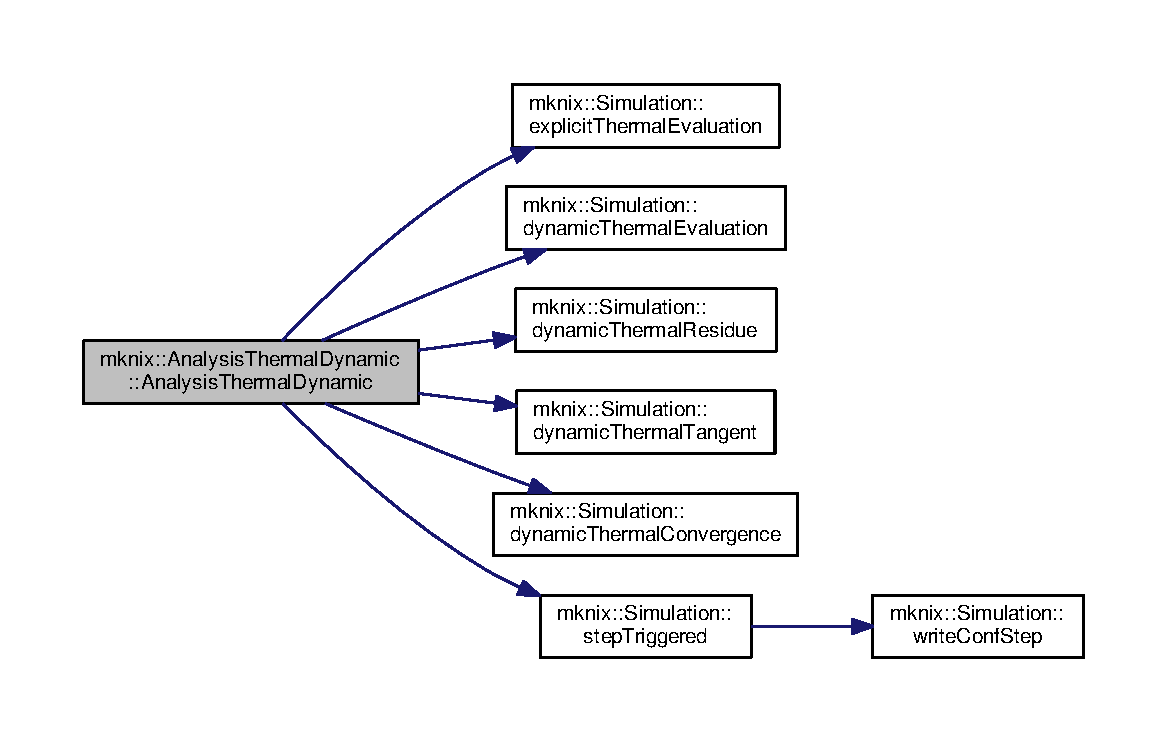
\includegraphics[width=350pt]{d5/dd9/classmknix_1_1_analysis_thermal_dynamic_a161ebe1ed696232ed05ef778cdcabcb8_cgraph}
\end{center}
\end{figure}


\hypertarget{classmknix_1_1_analysis_thermal_dynamic_ad0dbaa6affc6e4a285d310e209fe2b73}{}\index{mknix\+::\+Analysis\+Thermal\+Dynamic@{mknix\+::\+Analysis\+Thermal\+Dynamic}!````~Analysis\+Thermal\+Dynamic@{$\sim$\+Analysis\+Thermal\+Dynamic}}
\index{````~Analysis\+Thermal\+Dynamic@{$\sim$\+Analysis\+Thermal\+Dynamic}!mknix\+::\+Analysis\+Thermal\+Dynamic@{mknix\+::\+Analysis\+Thermal\+Dynamic}}
\paragraph[{$\sim$\+Analysis\+Thermal\+Dynamic}]{\setlength{\rightskip}{0pt plus 5cm}mknix\+::\+Analysis\+Thermal\+Dynamic\+::$\sim$\+Analysis\+Thermal\+Dynamic (
\begin{DoxyParamCaption}
{}
\end{DoxyParamCaption}
)}\label{classmknix_1_1_analysis_thermal_dynamic_ad0dbaa6affc6e4a285d310e209fe2b73}


Definition at line 64 of file analysisthermaldynamic.\+cpp.



\subsubsection{Member Function Documentation}
\hypertarget{classmknix_1_1_analysis_thermal_dynamic_a616aac65d4489996979a0c9120089e37}{}\index{mknix\+::\+Analysis\+Thermal\+Dynamic@{mknix\+::\+Analysis\+Thermal\+Dynamic}!init@{init}}
\index{init@{init}!mknix\+::\+Analysis\+Thermal\+Dynamic@{mknix\+::\+Analysis\+Thermal\+Dynamic}}
\paragraph[{init}]{\setlength{\rightskip}{0pt plus 5cm}void mknix\+::\+Analysis\+Thermal\+Dynamic\+::init (
\begin{DoxyParamCaption}
\item[{{\bf lmx\+::\+Vector}$<$ {\bf data\+\_\+type} $>$ $\ast$}]{qt\+\_\+in}
\end{DoxyParamCaption}
)\hspace{0.3cm}{\ttfamily [virtual]}}\label{classmknix_1_1_analysis_thermal_dynamic_a616aac65d4489996979a0c9120089e37}


Reimplemented from \hyperlink{classmknix_1_1_analysis_af9e3f13a8644466d416c7666a93c21ca}{mknix\+::\+Analysis}.



Definition at line 68 of file analysisthermaldynamic.\+cpp.

\hypertarget{classmknix_1_1_analysis_thermal_dynamic_a2c5b1abfa4cfbfea523e27286146fe77}{}\index{mknix\+::\+Analysis\+Thermal\+Dynamic@{mknix\+::\+Analysis\+Thermal\+Dynamic}!next\+Step@{next\+Step}}
\index{next\+Step@{next\+Step}!mknix\+::\+Analysis\+Thermal\+Dynamic@{mknix\+::\+Analysis\+Thermal\+Dynamic}}
\paragraph[{next\+Step}]{\setlength{\rightskip}{0pt plus 5cm}void mknix\+::\+Analysis\+Thermal\+Dynamic\+::next\+Step (
\begin{DoxyParamCaption}
{}
\end{DoxyParamCaption}
)\hspace{0.3cm}{\ttfamily [virtual]}}\label{classmknix_1_1_analysis_thermal_dynamic_a2c5b1abfa4cfbfea523e27286146fe77}


Reimplemented from \hyperlink{classmknix_1_1_analysis_a238dc1446726315d1d988c2b8eeda8e5}{mknix\+::\+Analysis}.



Definition at line 77 of file analysisthermaldynamic.\+cpp.

\hypertarget{classmknix_1_1_analysis_thermal_dynamic_a17a9d48a88a1268960dc15371ab703a7}{}\index{mknix\+::\+Analysis\+Thermal\+Dynamic@{mknix\+::\+Analysis\+Thermal\+Dynamic}!solve@{solve}}
\index{solve@{solve}!mknix\+::\+Analysis\+Thermal\+Dynamic@{mknix\+::\+Analysis\+Thermal\+Dynamic}}
\paragraph[{solve}]{\setlength{\rightskip}{0pt plus 5cm}void mknix\+::\+Analysis\+Thermal\+Dynamic\+::solve (
\begin{DoxyParamCaption}
\item[{{\bf lmx\+::\+Vector}$<$ {\bf data\+\_\+type} $>$ $\ast$}]{qt\+\_\+in, }
\item[{{\bf lmx\+::\+Vector}$<$ {\bf data\+\_\+type} $>$ $\ast$}]{qdot\+\_\+in = {\ttfamily 0}, }
\item[{{\bf lmx\+::\+Vector}$<$ {\bf data\+\_\+type} $>$ $\ast$}]{not\+\_\+used = {\ttfamily 0}}
\end{DoxyParamCaption}
)\hspace{0.3cm}{\ttfamily [virtual]}}\label{classmknix_1_1_analysis_thermal_dynamic_a17a9d48a88a1268960dc15371ab703a7}


Implements \hyperlink{classmknix_1_1_analysis_a515bc01fa8704395d310c5e7ebd45081}{mknix\+::\+Analysis}.



Definition at line 83 of file analysisthermaldynamic.\+cpp.

\hypertarget{classmknix_1_1_analysis_thermal_dynamic_ae1d271bfca189706a101259cff192ec9}{}\index{mknix\+::\+Analysis\+Thermal\+Dynamic@{mknix\+::\+Analysis\+Thermal\+Dynamic}!type@{type}}
\index{type@{type}!mknix\+::\+Analysis\+Thermal\+Dynamic@{mknix\+::\+Analysis\+Thermal\+Dynamic}}
\paragraph[{type}]{\setlength{\rightskip}{0pt plus 5cm}std\+::string mknix\+::\+Analysis\+Thermal\+Dynamic\+::type (
\begin{DoxyParamCaption}
{}
\end{DoxyParamCaption}
)\hspace{0.3cm}{\ttfamily [inline]}, {\ttfamily [virtual]}}\label{classmknix_1_1_analysis_thermal_dynamic_ae1d271bfca189706a101259cff192ec9}


Implements \hyperlink{classmknix_1_1_analysis_a6dd7026a22ae11f3eef3dad3be370e70}{mknix\+::\+Analysis}.



Definition at line 39 of file analysisthermaldynamic.\+h.



The documentation for this class was generated from the following files\+:\begin{DoxyCompactItemize}
\item 
\hyperlink{analysisthermaldynamic_8h}{analysisthermaldynamic.\+h}\item 
\hyperlink{analysisthermaldynamic_8cpp}{analysisthermaldynamic.\+cpp}\end{DoxyCompactItemize}

\hypertarget{classmknix_1_1_analysis_thermal_static}{}\subsection{mknix\+:\+:Analysis\+Thermal\+Static Class Reference}
\label{classmknix_1_1_analysis_thermal_static}\index{mknix\+::\+Analysis\+Thermal\+Static@{mknix\+::\+Analysis\+Thermal\+Static}}


{\ttfamily \#include $<$analysisthermalstatic.\+h$>$}



Inheritance diagram for mknix\+:\+:Analysis\+Thermal\+Static\+:\nopagebreak
\begin{figure}[H]
\begin{center}
\leavevmode
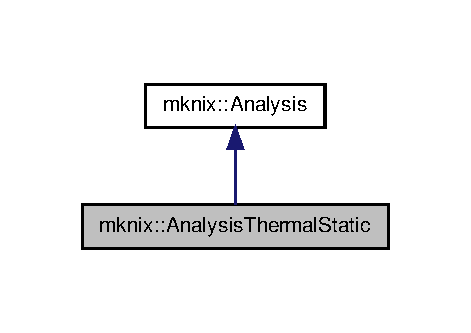
\includegraphics[width=227pt]{d1/df3/classmknix_1_1_analysis_thermal_static__inherit__graph}
\end{center}
\end{figure}


Collaboration diagram for mknix\+:\+:Analysis\+Thermal\+Static\+:\nopagebreak
\begin{figure}[H]
\begin{center}
\leavevmode
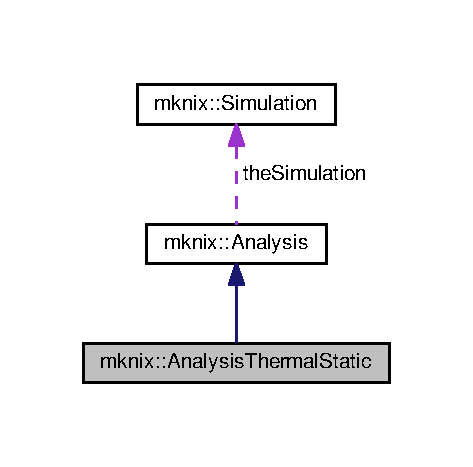
\includegraphics[width=227pt]{d1/d71/classmknix_1_1_analysis_thermal_static__coll__graph}
\end{center}
\end{figure}
\subsubsection*{Public Member Functions}
\begin{DoxyCompactItemize}
\item 
\hyperlink{classmknix_1_1_analysis_thermal_static_ae789aef70fc130d8478e09374e2541f5}{Analysis\+Thermal\+Static} ()
\item 
\hyperlink{classmknix_1_1_analysis_thermal_static_a340001a574c5c2ad92020c6bc8b99602}{Analysis\+Thermal\+Static} (\hyperlink{classmknix_1_1_simulation}{Simulation} $\ast$, double)
\item 
\hyperlink{classmknix_1_1_analysis_thermal_static_a0164991e5c2829051b9e886cb07e3af7}{$\sim$\+Analysis\+Thermal\+Static} ()
\item 
std\+::string \hyperlink{classmknix_1_1_analysis_thermal_static_a14a7b53403f7523ccb783129e928241b}{type} ()
\item 
void \hyperlink{classmknix_1_1_analysis_thermal_static_aa33ce60d449fbcffbfb0e4fdb7cfaa4a}{solve} (\hyperlink{classlmx_1_1_vector}{lmx\+::\+Vector}$<$ \hyperlink{namespacemknix_a16be4b246fbf2cceb141e3a179111020}{data\+\_\+type} $>$ $\ast$, \hyperlink{classlmx_1_1_vector}{lmx\+::\+Vector}$<$ \hyperlink{namespacemknix_a16be4b246fbf2cceb141e3a179111020}{data\+\_\+type} $>$ $\ast$, \hyperlink{classlmx_1_1_vector}{lmx\+::\+Vector}$<$ \hyperlink{namespacemknix_a16be4b246fbf2cceb141e3a179111020}{data\+\_\+type} $>$ $\ast$)
\end{DoxyCompactItemize}
\subsubsection*{Additional Inherited Members}


\subsubsection{Detailed Description}
\begin{DoxyAuthor}{Author}
A\+U\+T\+H\+O\+R\+S $<$\+M\+A\+I\+L\+S$>$ 
\end{DoxyAuthor}


Definition at line 30 of file analysisthermalstatic.\+h.



\subsubsection{Constructor \& Destructor Documentation}
\hypertarget{classmknix_1_1_analysis_thermal_static_ae789aef70fc130d8478e09374e2541f5}{}\index{mknix\+::\+Analysis\+Thermal\+Static@{mknix\+::\+Analysis\+Thermal\+Static}!Analysis\+Thermal\+Static@{Analysis\+Thermal\+Static}}
\index{Analysis\+Thermal\+Static@{Analysis\+Thermal\+Static}!mknix\+::\+Analysis\+Thermal\+Static@{mknix\+::\+Analysis\+Thermal\+Static}}
\paragraph[{Analysis\+Thermal\+Static}]{\setlength{\rightskip}{0pt plus 5cm}mknix\+::\+Analysis\+Thermal\+Static\+::\+Analysis\+Thermal\+Static (
\begin{DoxyParamCaption}
{}
\end{DoxyParamCaption}
)}\label{classmknix_1_1_analysis_thermal_static_ae789aef70fc130d8478e09374e2541f5}


Definition at line 25 of file analysisthermalstatic.\+cpp.

\hypertarget{classmknix_1_1_analysis_thermal_static_a340001a574c5c2ad92020c6bc8b99602}{}\index{mknix\+::\+Analysis\+Thermal\+Static@{mknix\+::\+Analysis\+Thermal\+Static}!Analysis\+Thermal\+Static@{Analysis\+Thermal\+Static}}
\index{Analysis\+Thermal\+Static@{Analysis\+Thermal\+Static}!mknix\+::\+Analysis\+Thermal\+Static@{mknix\+::\+Analysis\+Thermal\+Static}}
\paragraph[{Analysis\+Thermal\+Static}]{\setlength{\rightskip}{0pt plus 5cm}mknix\+::\+Analysis\+Thermal\+Static\+::\+Analysis\+Thermal\+Static (
\begin{DoxyParamCaption}
\item[{{\bf Simulation} $\ast$}]{simulation\+\_\+in, }
\item[{double}]{time\+\_\+in}
\end{DoxyParamCaption}
)}\label{classmknix_1_1_analysis_thermal_static_a340001a574c5c2ad92020c6bc8b99602}


Definition at line 31 of file analysisthermalstatic.\+cpp.



Here is the call graph for this function\+:\nopagebreak
\begin{figure}[H]
\begin{center}
\leavevmode
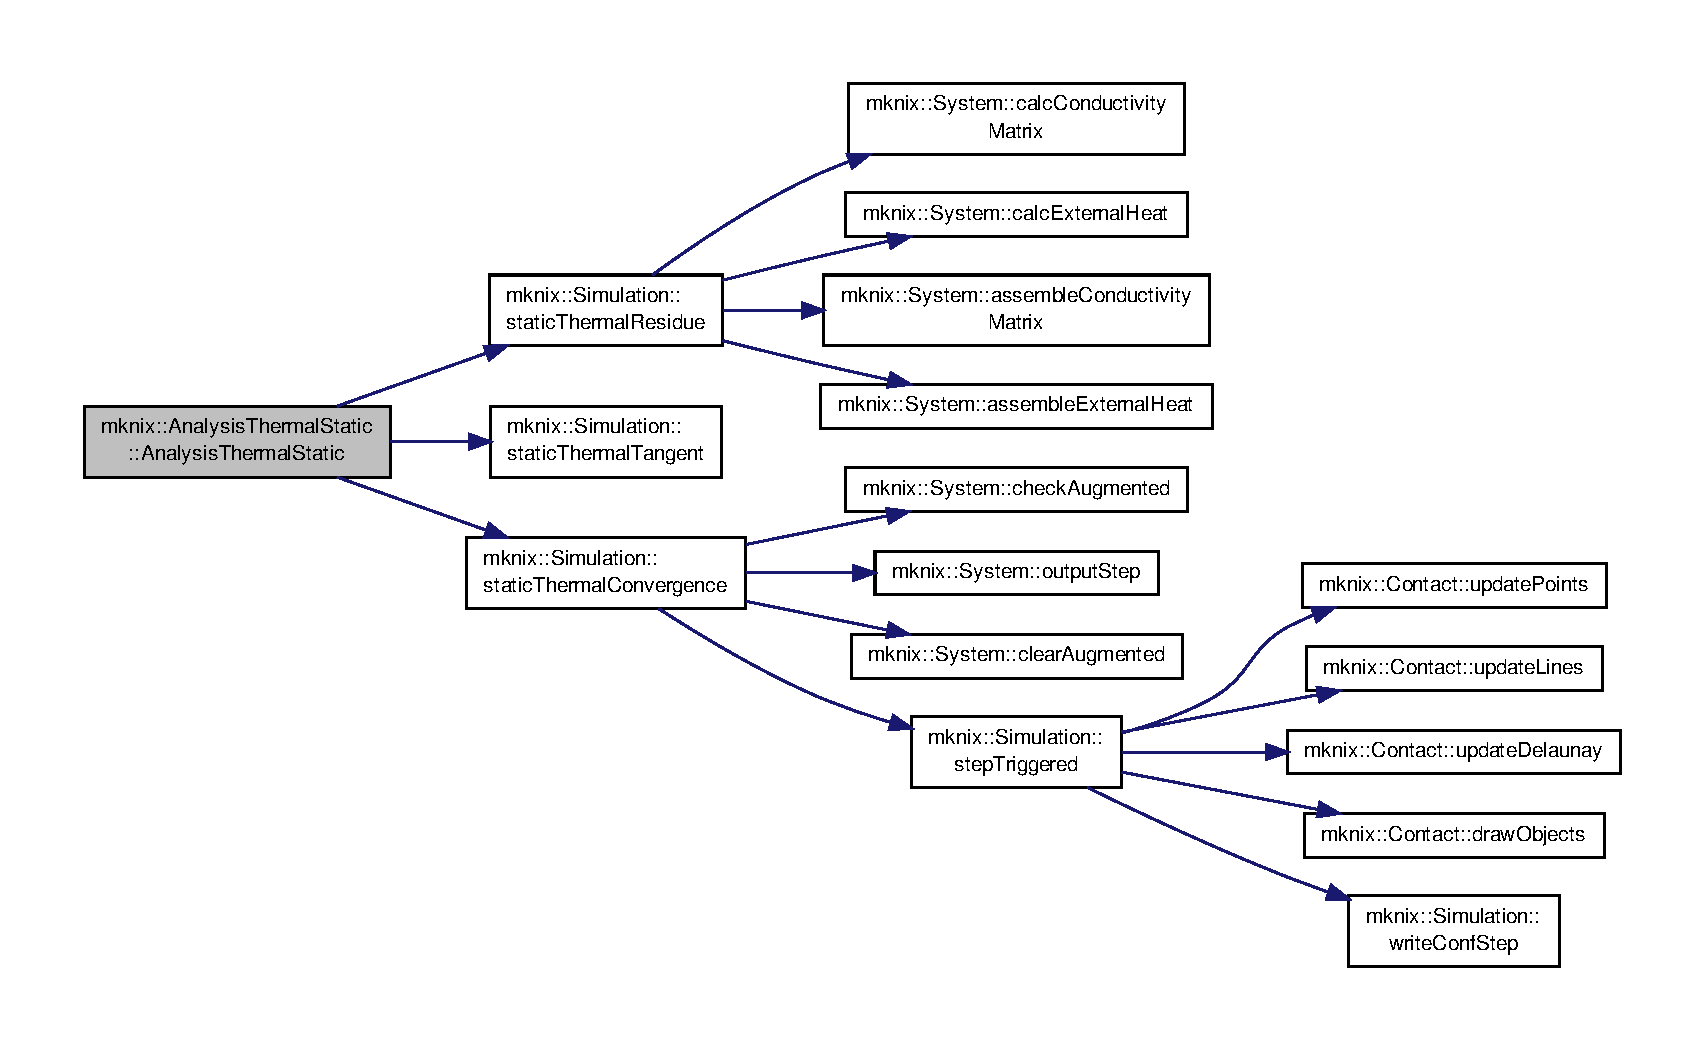
\includegraphics[width=350pt]{d4/d3e/classmknix_1_1_analysis_thermal_static_a340001a574c5c2ad92020c6bc8b99602_cgraph}
\end{center}
\end{figure}


\hypertarget{classmknix_1_1_analysis_thermal_static_a0164991e5c2829051b9e886cb07e3af7}{}\index{mknix\+::\+Analysis\+Thermal\+Static@{mknix\+::\+Analysis\+Thermal\+Static}!````~Analysis\+Thermal\+Static@{$\sim$\+Analysis\+Thermal\+Static}}
\index{````~Analysis\+Thermal\+Static@{$\sim$\+Analysis\+Thermal\+Static}!mknix\+::\+Analysis\+Thermal\+Static@{mknix\+::\+Analysis\+Thermal\+Static}}
\paragraph[{$\sim$\+Analysis\+Thermal\+Static}]{\setlength{\rightskip}{0pt plus 5cm}mknix\+::\+Analysis\+Thermal\+Static\+::$\sim$\+Analysis\+Thermal\+Static (
\begin{DoxyParamCaption}
{}
\end{DoxyParamCaption}
)}\label{classmknix_1_1_analysis_thermal_static_a0164991e5c2829051b9e886cb07e3af7}


Definition at line 43 of file analysisthermalstatic.\+cpp.



\subsubsection{Member Function Documentation}
\hypertarget{classmknix_1_1_analysis_thermal_static_aa33ce60d449fbcffbfb0e4fdb7cfaa4a}{}\index{mknix\+::\+Analysis\+Thermal\+Static@{mknix\+::\+Analysis\+Thermal\+Static}!solve@{solve}}
\index{solve@{solve}!mknix\+::\+Analysis\+Thermal\+Static@{mknix\+::\+Analysis\+Thermal\+Static}}
\paragraph[{solve}]{\setlength{\rightskip}{0pt plus 5cm}void mknix\+::\+Analysis\+Thermal\+Static\+::solve (
\begin{DoxyParamCaption}
\item[{{\bf lmx\+::\+Vector}$<$ {\bf data\+\_\+type} $>$ $\ast$}]{q\+\_\+in, }
\item[{{\bf lmx\+::\+Vector}$<$ {\bf data\+\_\+type} $>$ $\ast$}]{qdot\+\_\+in = {\ttfamily 0}, }
\item[{{\bf lmx\+::\+Vector}$<$ {\bf data\+\_\+type} $>$ $\ast$}]{not\+\_\+used = {\ttfamily 0}}
\end{DoxyParamCaption}
)\hspace{0.3cm}{\ttfamily [virtual]}}\label{classmknix_1_1_analysis_thermal_static_aa33ce60d449fbcffbfb0e4fdb7cfaa4a}


Implements \hyperlink{classmknix_1_1_analysis_a515bc01fa8704395d310c5e7ebd45081}{mknix\+::\+Analysis}.



Definition at line 48 of file analysisthermalstatic.\+cpp.

\hypertarget{classmknix_1_1_analysis_thermal_static_a14a7b53403f7523ccb783129e928241b}{}\index{mknix\+::\+Analysis\+Thermal\+Static@{mknix\+::\+Analysis\+Thermal\+Static}!type@{type}}
\index{type@{type}!mknix\+::\+Analysis\+Thermal\+Static@{mknix\+::\+Analysis\+Thermal\+Static}}
\paragraph[{type}]{\setlength{\rightskip}{0pt plus 5cm}std\+::string mknix\+::\+Analysis\+Thermal\+Static\+::type (
\begin{DoxyParamCaption}
{}
\end{DoxyParamCaption}
)\hspace{0.3cm}{\ttfamily [inline]}, {\ttfamily [virtual]}}\label{classmknix_1_1_analysis_thermal_static_a14a7b53403f7523ccb783129e928241b}


Implements \hyperlink{classmknix_1_1_analysis_a6dd7026a22ae11f3eef3dad3be370e70}{mknix\+::\+Analysis}.



Definition at line 39 of file analysisthermalstatic.\+h.



The documentation for this class was generated from the following files\+:\begin{DoxyCompactItemize}
\item 
\hyperlink{analysisthermalstatic_8h}{analysisthermalstatic.\+h}\item 
\hyperlink{analysisthermalstatic_8cpp}{analysisthermalstatic.\+cpp}\end{DoxyCompactItemize}

\hypertarget{classmknix_1_1_body}{\subsection{mknix\-:\-:Body Class Reference}
\label{classmknix_1_1_body}\index{mknix\-::\-Body@{mknix\-::\-Body}}
}


{\ttfamily \#include $<$body.\-h$>$}



Inheritance diagram for mknix\-:\-:Body\-:\nopagebreak
\begin{figure}[H]
\begin{center}
\leavevmode
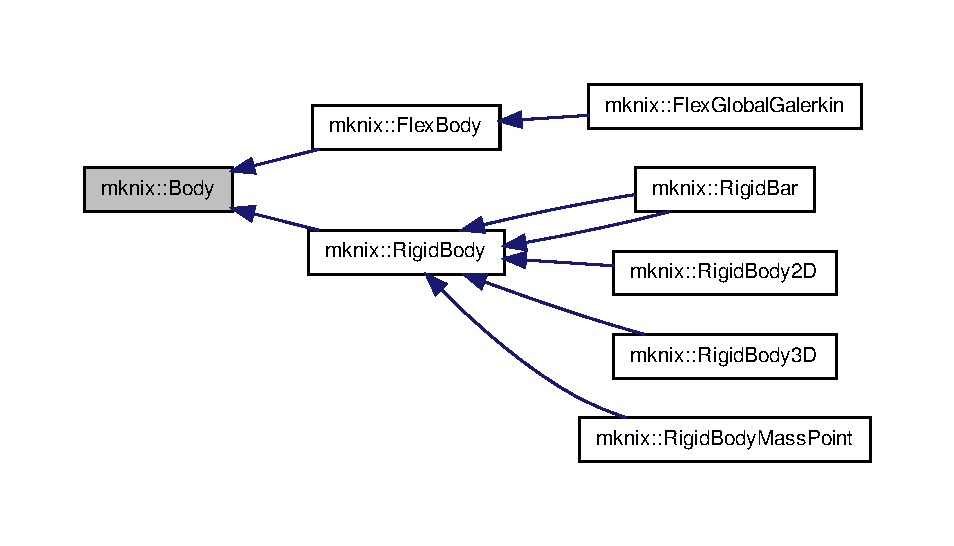
\includegraphics[width=350pt]{d9/d1c/classmknix_1_1_body__inherit__graph}
\end{center}
\end{figure}
\subsubsection*{Public Member Functions}
\begin{DoxyCompactItemize}
\item 
\hyperlink{classmknix_1_1_body_a5f11ba30f14169c567d8e3f84afbbf40}{Body} ()
\item 
\hyperlink{classmknix_1_1_body_a121c49df553ac35ca246052168eccb7f}{Body} (std\-::string)
\item 
virtual \hyperlink{classmknix_1_1_body_ad58a0a50a821e1adaa5abd1320e5a837}{$\sim$\-Body} ()
\item 
virtual std\-::string \hyperlink{classmknix_1_1_body_a603ed0a11eee91957b2655a0e4667cd4}{get\-Type} ()=0
\item 
virtual void \hyperlink{classmknix_1_1_body_ad34fa07c6620c9fcc2268bfdbfd42194}{calc\-Mass\-Matrix} ()=0
\item 
virtual void \hyperlink{classmknix_1_1_body_a71d21e817523058098bcec62fb377187}{calc\-External\-Forces} ()=0
\item 
virtual void \hyperlink{classmknix_1_1_body_acd6c47f4e0a25e927141cb325df896a9}{assemble\-Mass\-Matrix} (lmx\-::\-Matrix$<$ \hyperlink{namespacemknix_a16be4b246fbf2cceb141e3a179111020}{data\-\_\-type} $>$ \&)=0
\item 
virtual void \hyperlink{classmknix_1_1_body_a46a17ef341d6ea217e1548108a4e9efc}{assemble\-External\-Forces} (lmx\-::\-Vector$<$ \hyperlink{namespacemknix_a16be4b246fbf2cceb141e3a179111020}{data\-\_\-type} $>$ \&)=0
\item 
virtual void \hyperlink{classmknix_1_1_body_a689970a0729d557ed56492bbfeae4ecd}{set\-Output} (std\-::string)=0
\item 
virtual void \hyperlink{classmknix_1_1_body_a2655307ec61a79f8d2e5716c984a44df}{output\-Step} (const lmx\-::\-Vector$<$ \hyperlink{namespacemknix_a16be4b246fbf2cceb141e3a179111020}{data\-\_\-type} $>$ \&, const lmx\-::\-Vector$<$ \hyperlink{namespacemknix_a16be4b246fbf2cceb141e3a179111020}{data\-\_\-type} $>$ \&)=0
\item 
virtual void \hyperlink{classmknix_1_1_body_a0570075194360f453b763866969548e7}{output\-Step} (const lmx\-::\-Vector$<$ \hyperlink{namespacemknix_a16be4b246fbf2cceb141e3a179111020}{data\-\_\-type} $>$ \&)=0
\item 
virtual void \hyperlink{classmknix_1_1_body_acc0dd60d384ec11bf1ea71fed9ae27b3}{output\-To\-File} (std\-::ofstream $\ast$)=0
\item 
virtual void \hyperlink{classmknix_1_1_body_abf7eec507e5fc918e4901864a6db0f84}{add\-Node} (\hyperlink{classmknix_1_1_node}{Node} $\ast$node\-\_\-in)
\item 
\hyperlink{classmknix_1_1_node}{Node} $\ast$ \hyperlink{classmknix_1_1_body_ac996b024251ecd5bcb9af4a932e916c2}{get\-Node} (int node\-\_\-number)
\item 
virtual \hyperlink{classmknix_1_1_node}{Node} $\ast$ \hyperlink{classmknix_1_1_body_a95fad3fdd4c18a0adcbeba2891b55140}{get\-Last\-Node} ()
\item 
virtual void \hyperlink{classmknix_1_1_body_a0303c5d1de1c19cff7448baf2564f213}{add\-Boundary\-Line} (\hyperlink{classmknix_1_1_node}{Node} $\ast$node1, \hyperlink{classmknix_1_1_node}{Node} $\ast$node2)
\item 
virtual int \hyperlink{classmknix_1_1_body_aa7de934eb85ec4e68741d0c7395a9a10}{get\-Boundary\-Size} ()
\item 
virtual \hyperlink{classmknix_1_1_node}{Node} $\ast$ \hyperlink{classmknix_1_1_body_a0cd2969a179a3d6a44607e038593028b}{get\-Boundary\-First\-Node} ()
\item 
virtual \hyperlink{classmknix_1_1_node}{Node} $\ast$ \hyperlink{classmknix_1_1_body_aac3a9453cb1a13464fa56449112188f1}{get\-Boundary\-Next\-Node} (\hyperlink{classmknix_1_1_node}{Node} $\ast$node\-\_\-in)
\item 
virtual void \hyperlink{classmknix_1_1_body_abb4237e7f457287766e29bfe0cbb0f01}{add\-Cell} (int num, \hyperlink{classmknix_1_1_cell}{Cell} $\ast$cell\-\_\-in)
\item 
virtual void \hyperlink{classmknix_1_1_body_ada574d09e98568156185eb7eef398c8f}{write\-Boundary\-Nodes} (std\-::vector$<$ \hyperlink{classmknix_1_1_node}{Node} $\ast$ $>$ \&)=0
\item 
virtual void \hyperlink{classmknix_1_1_body_ab95b00050cf3841c1b931e04eebe57e1}{write\-Boundary\-Connectivity} (std\-::vector$<$ std\-::vector$<$ \hyperlink{classmknix_1_1_node}{Node} $\ast$ $>$ $>$ \&)=0
\item 
virtual void \hyperlink{classmknix_1_1_body_a5f58f8e5398bbacc973b046be600eb5f}{translate} (double, double, double)
\end{DoxyCompactItemize}
\subsubsection*{Protected Attributes}
\begin{DoxyCompactItemize}
\item 
std\-::string \hyperlink{classmknix_1_1_body_a3c05cdff2d5f2b150046cd734d0ed7ce}{title}
\item 
std\-::vector$<$ \hyperlink{classmknix_1_1_node}{Node} $\ast$ $>$ \hyperlink{classmknix_1_1_body_a3393da3459cbf7b35ee3dedb982180bf}{nodes}
\item 
std\-::map$<$ \hyperlink{classmknix_1_1_node}{Node} $\ast$, \hyperlink{classmknix_1_1_node}{Node} $\ast$ $>$ \hyperlink{classmknix_1_1_body_abaacc346d058cdabb8d0273b1440e323}{boundary}
\item 
std\-::map$<$ int, \hyperlink{classmknix_1_1_cell}{Cell} $\ast$ $>$ \hyperlink{classmknix_1_1_body_afa538e2bc24cd6623e63b44704037a73}{cells}
\item 
lmx\-::\-Matrix$<$ \hyperlink{namespacemknix_a16be4b246fbf2cceb141e3a179111020}{data\-\_\-type} $>$ \hyperlink{classmknix_1_1_body_abf69d9fd5ede2c511d85c5d644902c6e}{local\-Mass\-Matrix}
\end{DoxyCompactItemize}


\subsubsection{Detailed Description}
\begin{DoxyAuthor}{Author}
A\-U\-T\-H\-O\-R\-S $<$\-M\-A\-I\-L\-S$>$ 
\end{DoxyAuthor}


\subsubsection{Constructor \& Destructor Documentation}
\hypertarget{classmknix_1_1_body_a5f11ba30f14169c567d8e3f84afbbf40}{\index{mknix\-::\-Body@{mknix\-::\-Body}!Body@{Body}}
\index{Body@{Body}!mknix::Body@{mknix\-::\-Body}}
\paragraph[{Body}]{\setlength{\rightskip}{0pt plus 5cm}mknix\-::\-Body\-::\-Body (
\begin{DoxyParamCaption}
{}
\end{DoxyParamCaption}
)}}\label{classmknix_1_1_body_a5f11ba30f14169c567d8e3f84afbbf40}
\hypertarget{classmknix_1_1_body_a121c49df553ac35ca246052168eccb7f}{\index{mknix\-::\-Body@{mknix\-::\-Body}!Body@{Body}}
\index{Body@{Body}!mknix::Body@{mknix\-::\-Body}}
\paragraph[{Body}]{\setlength{\rightskip}{0pt plus 5cm}mknix\-::\-Body\-::\-Body (
\begin{DoxyParamCaption}
\item[{std\-::string}]{title\-\_\-in}
\end{DoxyParamCaption}
)}}\label{classmknix_1_1_body_a121c49df553ac35ca246052168eccb7f}
\hypertarget{classmknix_1_1_body_ad58a0a50a821e1adaa5abd1320e5a837}{\index{mknix\-::\-Body@{mknix\-::\-Body}!$\sim$\-Body@{$\sim$\-Body}}
\index{$\sim$\-Body@{$\sim$\-Body}!mknix::Body@{mknix\-::\-Body}}
\paragraph[{$\sim$\-Body}]{\setlength{\rightskip}{0pt plus 5cm}mknix\-::\-Body\-::$\sim$\-Body (
\begin{DoxyParamCaption}
{}
\end{DoxyParamCaption}
)\hspace{0.3cm}{\ttfamily [virtual]}}}\label{classmknix_1_1_body_ad58a0a50a821e1adaa5abd1320e5a837}


\subsubsection{Member Function Documentation}
\hypertarget{classmknix_1_1_body_a0303c5d1de1c19cff7448baf2564f213}{\index{mknix\-::\-Body@{mknix\-::\-Body}!add\-Boundary\-Line@{add\-Boundary\-Line}}
\index{add\-Boundary\-Line@{add\-Boundary\-Line}!mknix::Body@{mknix\-::\-Body}}
\paragraph[{add\-Boundary\-Line}]{\setlength{\rightskip}{0pt plus 5cm}virtual void mknix\-::\-Body\-::add\-Boundary\-Line (
\begin{DoxyParamCaption}
\item[{{\bf Node} $\ast$}]{node1, }
\item[{{\bf Node} $\ast$}]{node2}
\end{DoxyParamCaption}
)\hspace{0.3cm}{\ttfamily [inline]}, {\ttfamily [virtual]}}}\label{classmknix_1_1_body_a0303c5d1de1c19cff7448baf2564f213}
\hypertarget{classmknix_1_1_body_abb4237e7f457287766e29bfe0cbb0f01}{\index{mknix\-::\-Body@{mknix\-::\-Body}!add\-Cell@{add\-Cell}}
\index{add\-Cell@{add\-Cell}!mknix::Body@{mknix\-::\-Body}}
\paragraph[{add\-Cell}]{\setlength{\rightskip}{0pt plus 5cm}virtual void mknix\-::\-Body\-::add\-Cell (
\begin{DoxyParamCaption}
\item[{int}]{num, }
\item[{{\bf Cell} $\ast$}]{cell\-\_\-in}
\end{DoxyParamCaption}
)\hspace{0.3cm}{\ttfamily [inline]}, {\ttfamily [virtual]}}}\label{classmknix_1_1_body_abb4237e7f457287766e29bfe0cbb0f01}
\hypertarget{classmknix_1_1_body_abf7eec507e5fc918e4901864a6db0f84}{\index{mknix\-::\-Body@{mknix\-::\-Body}!add\-Node@{add\-Node}}
\index{add\-Node@{add\-Node}!mknix::Body@{mknix\-::\-Body}}
\paragraph[{add\-Node}]{\setlength{\rightskip}{0pt plus 5cm}virtual void mknix\-::\-Body\-::add\-Node (
\begin{DoxyParamCaption}
\item[{{\bf Node} $\ast$}]{node\-\_\-in}
\end{DoxyParamCaption}
)\hspace{0.3cm}{\ttfamily [inline]}, {\ttfamily [virtual]}}}\label{classmknix_1_1_body_abf7eec507e5fc918e4901864a6db0f84}


Reimplemented in \hyperlink{classmknix_1_1_rigid_bar_a1f05aae37c654229c4f6c3ef32944125}{mknix\-::\-Rigid\-Bar}, and \hyperlink{classmknix_1_1_rigid_body_a88b0dfc0af5002ee8d060df5e520434f}{mknix\-::\-Rigid\-Body}.

\hypertarget{classmknix_1_1_body_a46a17ef341d6ea217e1548108a4e9efc}{\index{mknix\-::\-Body@{mknix\-::\-Body}!assemble\-External\-Forces@{assemble\-External\-Forces}}
\index{assemble\-External\-Forces@{assemble\-External\-Forces}!mknix::Body@{mknix\-::\-Body}}
\paragraph[{assemble\-External\-Forces}]{\setlength{\rightskip}{0pt plus 5cm}virtual void mknix\-::\-Body\-::assemble\-External\-Forces (
\begin{DoxyParamCaption}
\item[{lmx\-::\-Vector$<$ {\bf data\-\_\-type} $>$ \&}]{}
\end{DoxyParamCaption}
)\hspace{0.3cm}{\ttfamily [pure virtual]}}}\label{classmknix_1_1_body_a46a17ef341d6ea217e1548108a4e9efc}


Implemented in \hyperlink{classmknix_1_1_flex_global_galerkin_acc0254dbedc2543be9051aab1acb7d99}{mknix\-::\-Flex\-Global\-Galerkin}, and \hyperlink{classmknix_1_1_rigid_body_a18c7ffa5b9f2d3df008a92f421404fac}{mknix\-::\-Rigid\-Body}.

\hypertarget{classmknix_1_1_body_acd6c47f4e0a25e927141cb325df896a9}{\index{mknix\-::\-Body@{mknix\-::\-Body}!assemble\-Mass\-Matrix@{assemble\-Mass\-Matrix}}
\index{assemble\-Mass\-Matrix@{assemble\-Mass\-Matrix}!mknix::Body@{mknix\-::\-Body}}
\paragraph[{assemble\-Mass\-Matrix}]{\setlength{\rightskip}{0pt plus 5cm}virtual void mknix\-::\-Body\-::assemble\-Mass\-Matrix (
\begin{DoxyParamCaption}
\item[{lmx\-::\-Matrix$<$ {\bf data\-\_\-type} $>$ \&}]{}
\end{DoxyParamCaption}
)\hspace{0.3cm}{\ttfamily [pure virtual]}}}\label{classmknix_1_1_body_acd6c47f4e0a25e927141cb325df896a9}


Implemented in \hyperlink{classmknix_1_1_flex_global_galerkin_a689a56babe9734eb504a9c948b6a3587}{mknix\-::\-Flex\-Global\-Galerkin}, and \hyperlink{classmknix_1_1_rigid_body_ac20200b40e6e222261bb8257e339d7b4}{mknix\-::\-Rigid\-Body}.

\hypertarget{classmknix_1_1_body_a71d21e817523058098bcec62fb377187}{\index{mknix\-::\-Body@{mknix\-::\-Body}!calc\-External\-Forces@{calc\-External\-Forces}}
\index{calc\-External\-Forces@{calc\-External\-Forces}!mknix::Body@{mknix\-::\-Body}}
\paragraph[{calc\-External\-Forces}]{\setlength{\rightskip}{0pt plus 5cm}virtual void mknix\-::\-Body\-::calc\-External\-Forces (
\begin{DoxyParamCaption}
{}
\end{DoxyParamCaption}
)\hspace{0.3cm}{\ttfamily [pure virtual]}}}\label{classmknix_1_1_body_a71d21e817523058098bcec62fb377187}


Implemented in \hyperlink{classmknix_1_1_flex_global_galerkin_a2ed7079f0f2674c3556ff8dbbf3a63d3}{mknix\-::\-Flex\-Global\-Galerkin}, \hyperlink{classmknix_1_1_rigid_body3_d_a66bff0110ce5d201875f068050c84c96}{mknix\-::\-Rigid\-Body3\-D}, \hyperlink{classmknix_1_1_rigid_body_mass_point_a281842fc7cf1367bbed4c5e477ac8da9}{mknix\-::\-Rigid\-Body\-Mass\-Point}, \hyperlink{classmknix_1_1_rigid_bar_a4325fbe1df7832ce09bd2bf72b00cf67}{mknix\-::\-Rigid\-Bar}, \hyperlink{classmknix_1_1_rigid_body2_d_a2d1b7d48c98c3e0ef63dc2c975637793}{mknix\-::\-Rigid\-Body2\-D}, and \hyperlink{classmknix_1_1_rigid_bar_a4325fbe1df7832ce09bd2bf72b00cf67}{mknix\-::\-Rigid\-Bar}.

\hypertarget{classmknix_1_1_body_ad34fa07c6620c9fcc2268bfdbfd42194}{\index{mknix\-::\-Body@{mknix\-::\-Body}!calc\-Mass\-Matrix@{calc\-Mass\-Matrix}}
\index{calc\-Mass\-Matrix@{calc\-Mass\-Matrix}!mknix::Body@{mknix\-::\-Body}}
\paragraph[{calc\-Mass\-Matrix}]{\setlength{\rightskip}{0pt plus 5cm}virtual void mknix\-::\-Body\-::calc\-Mass\-Matrix (
\begin{DoxyParamCaption}
{}
\end{DoxyParamCaption}
)\hspace{0.3cm}{\ttfamily [pure virtual]}}}\label{classmknix_1_1_body_ad34fa07c6620c9fcc2268bfdbfd42194}


Implemented in \hyperlink{classmknix_1_1_rigid_body3_d_a257d9b0bb9fe27664227270cd73194a4}{mknix\-::\-Rigid\-Body3\-D}, \hyperlink{classmknix_1_1_rigid_body_mass_point_aed37447f963c4393b30febe281589b99}{mknix\-::\-Rigid\-Body\-Mass\-Point}, \hyperlink{classmknix_1_1_flex_global_galerkin_ae5bb8c27e7494b233a96d971833a0d0d}{mknix\-::\-Flex\-Global\-Galerkin}, \hyperlink{classmknix_1_1_rigid_bar_a3d368a1a10b600179fbb7e901472c301}{mknix\-::\-Rigid\-Bar}, \hyperlink{classmknix_1_1_rigid_body2_d_a9ee8593743364a723107d307c12d8ad1}{mknix\-::\-Rigid\-Body2\-D}, and \hyperlink{classmknix_1_1_rigid_bar_a3d368a1a10b600179fbb7e901472c301}{mknix\-::\-Rigid\-Bar}.

\hypertarget{classmknix_1_1_body_a0cd2969a179a3d6a44607e038593028b}{\index{mknix\-::\-Body@{mknix\-::\-Body}!get\-Boundary\-First\-Node@{get\-Boundary\-First\-Node}}
\index{get\-Boundary\-First\-Node@{get\-Boundary\-First\-Node}!mknix::Body@{mknix\-::\-Body}}
\paragraph[{get\-Boundary\-First\-Node}]{\setlength{\rightskip}{0pt plus 5cm}virtual {\bf Node}$\ast$ mknix\-::\-Body\-::get\-Boundary\-First\-Node (
\begin{DoxyParamCaption}
{}
\end{DoxyParamCaption}
)\hspace{0.3cm}{\ttfamily [inline]}, {\ttfamily [virtual]}}}\label{classmknix_1_1_body_a0cd2969a179a3d6a44607e038593028b}
\hypertarget{classmknix_1_1_body_aac3a9453cb1a13464fa56449112188f1}{\index{mknix\-::\-Body@{mknix\-::\-Body}!get\-Boundary\-Next\-Node@{get\-Boundary\-Next\-Node}}
\index{get\-Boundary\-Next\-Node@{get\-Boundary\-Next\-Node}!mknix::Body@{mknix\-::\-Body}}
\paragraph[{get\-Boundary\-Next\-Node}]{\setlength{\rightskip}{0pt plus 5cm}virtual {\bf Node}$\ast$ mknix\-::\-Body\-::get\-Boundary\-Next\-Node (
\begin{DoxyParamCaption}
\item[{{\bf Node} $\ast$}]{node\-\_\-in}
\end{DoxyParamCaption}
)\hspace{0.3cm}{\ttfamily [inline]}, {\ttfamily [virtual]}}}\label{classmknix_1_1_body_aac3a9453cb1a13464fa56449112188f1}
\hypertarget{classmknix_1_1_body_aa7de934eb85ec4e68741d0c7395a9a10}{\index{mknix\-::\-Body@{mknix\-::\-Body}!get\-Boundary\-Size@{get\-Boundary\-Size}}
\index{get\-Boundary\-Size@{get\-Boundary\-Size}!mknix::Body@{mknix\-::\-Body}}
\paragraph[{get\-Boundary\-Size}]{\setlength{\rightskip}{0pt plus 5cm}virtual int mknix\-::\-Body\-::get\-Boundary\-Size (
\begin{DoxyParamCaption}
{}
\end{DoxyParamCaption}
)\hspace{0.3cm}{\ttfamily [inline]}, {\ttfamily [virtual]}}}\label{classmknix_1_1_body_aa7de934eb85ec4e68741d0c7395a9a10}
\hypertarget{classmknix_1_1_body_a95fad3fdd4c18a0adcbeba2891b55140}{\index{mknix\-::\-Body@{mknix\-::\-Body}!get\-Last\-Node@{get\-Last\-Node}}
\index{get\-Last\-Node@{get\-Last\-Node}!mknix::Body@{mknix\-::\-Body}}
\paragraph[{get\-Last\-Node}]{\setlength{\rightskip}{0pt plus 5cm}virtual {\bf Node}$\ast$ mknix\-::\-Body\-::get\-Last\-Node (
\begin{DoxyParamCaption}
{}
\end{DoxyParamCaption}
)\hspace{0.3cm}{\ttfamily [inline]}, {\ttfamily [virtual]}}}\label{classmknix_1_1_body_a95fad3fdd4c18a0adcbeba2891b55140}
\hypertarget{classmknix_1_1_body_ac996b024251ecd5bcb9af4a932e916c2}{\index{mknix\-::\-Body@{mknix\-::\-Body}!get\-Node@{get\-Node}}
\index{get\-Node@{get\-Node}!mknix::Body@{mknix\-::\-Body}}
\paragraph[{get\-Node}]{\setlength{\rightskip}{0pt plus 5cm}{\bf Node}$\ast$ mknix\-::\-Body\-::get\-Node (
\begin{DoxyParamCaption}
\item[{int}]{node\-\_\-number}
\end{DoxyParamCaption}
)\hspace{0.3cm}{\ttfamily [inline]}}}\label{classmknix_1_1_body_ac996b024251ecd5bcb9af4a932e916c2}
\hypertarget{classmknix_1_1_body_a603ed0a11eee91957b2655a0e4667cd4}{\index{mknix\-::\-Body@{mknix\-::\-Body}!get\-Type@{get\-Type}}
\index{get\-Type@{get\-Type}!mknix::Body@{mknix\-::\-Body}}
\paragraph[{get\-Type}]{\setlength{\rightskip}{0pt plus 5cm}virtual std\-::string mknix\-::\-Body\-::get\-Type (
\begin{DoxyParamCaption}
{}
\end{DoxyParamCaption}
)\hspace{0.3cm}{\ttfamily [pure virtual]}}}\label{classmknix_1_1_body_a603ed0a11eee91957b2655a0e4667cd4}


Implemented in \hyperlink{classmknix_1_1_rigid_body_mass_point_aa97f367f1f1701f5d7981c994a96fb5e}{mknix\-::\-Rigid\-Body\-Mass\-Point}, \hyperlink{classmknix_1_1_rigid_body3_d_a3cdb37910a3ed061017926d67932ad06}{mknix\-::\-Rigid\-Body3\-D}, \hyperlink{classmknix_1_1_rigid_bar_acc95a2895043626253a4bb8ee1eb341a}{mknix\-::\-Rigid\-Bar}, \hyperlink{classmknix_1_1_rigid_bar_acc95a2895043626253a4bb8ee1eb341a}{mknix\-::\-Rigid\-Bar}, \hyperlink{classmknix_1_1_rigid_body2_d_a36d7142c5123c4055c019109fb6169dc}{mknix\-::\-Rigid\-Body2\-D}, and \hyperlink{classmknix_1_1_flex_global_galerkin_a31c93b0ce740217ce4cd12e71646d8cf}{mknix\-::\-Flex\-Global\-Galerkin}.

\hypertarget{classmknix_1_1_body_a2655307ec61a79f8d2e5716c984a44df}{\index{mknix\-::\-Body@{mknix\-::\-Body}!output\-Step@{output\-Step}}
\index{output\-Step@{output\-Step}!mknix::Body@{mknix\-::\-Body}}
\paragraph[{output\-Step}]{\setlength{\rightskip}{0pt plus 5cm}virtual void mknix\-::\-Body\-::output\-Step (
\begin{DoxyParamCaption}
\item[{const lmx\-::\-Vector$<$ {\bf data\-\_\-type} $>$ \&}]{, }
\item[{const lmx\-::\-Vector$<$ {\bf data\-\_\-type} $>$ \&}]{}
\end{DoxyParamCaption}
)\hspace{0.3cm}{\ttfamily [pure virtual]}}}\label{classmknix_1_1_body_a2655307ec61a79f8d2e5716c984a44df}


Implemented in \hyperlink{classmknix_1_1_flex_global_galerkin_a031a130b73e3fe0fc862393f94d235cb}{mknix\-::\-Flex\-Global\-Galerkin}, and \hyperlink{classmknix_1_1_rigid_body_a721e9f81cfba9a3d425df36f7cf5ef71}{mknix\-::\-Rigid\-Body}.

\hypertarget{classmknix_1_1_body_a0570075194360f453b763866969548e7}{\index{mknix\-::\-Body@{mknix\-::\-Body}!output\-Step@{output\-Step}}
\index{output\-Step@{output\-Step}!mknix::Body@{mknix\-::\-Body}}
\paragraph[{output\-Step}]{\setlength{\rightskip}{0pt plus 5cm}virtual void mknix\-::\-Body\-::output\-Step (
\begin{DoxyParamCaption}
\item[{const lmx\-::\-Vector$<$ {\bf data\-\_\-type} $>$ \&}]{}
\end{DoxyParamCaption}
)\hspace{0.3cm}{\ttfamily [pure virtual]}}}\label{classmknix_1_1_body_a0570075194360f453b763866969548e7}


Implemented in \hyperlink{classmknix_1_1_flex_global_galerkin_a1882efa0a8f8c8832f6116b8f7874d2a}{mknix\-::\-Flex\-Global\-Galerkin}, and \hyperlink{classmknix_1_1_rigid_body_a605ed074fed7570c6620a6a6f6cd4bb0}{mknix\-::\-Rigid\-Body}.

\hypertarget{classmknix_1_1_body_acc0dd60d384ec11bf1ea71fed9ae27b3}{\index{mknix\-::\-Body@{mknix\-::\-Body}!output\-To\-File@{output\-To\-File}}
\index{output\-To\-File@{output\-To\-File}!mknix::Body@{mknix\-::\-Body}}
\paragraph[{output\-To\-File}]{\setlength{\rightskip}{0pt plus 5cm}virtual void mknix\-::\-Body\-::output\-To\-File (
\begin{DoxyParamCaption}
\item[{std\-::ofstream $\ast$}]{}
\end{DoxyParamCaption}
)\hspace{0.3cm}{\ttfamily [pure virtual]}}}\label{classmknix_1_1_body_acc0dd60d384ec11bf1ea71fed9ae27b3}


Implemented in \hyperlink{classmknix_1_1_flex_body_a1cf57f024248bbb196e91aac9b9ab9fe}{mknix\-::\-Flex\-Body}, and \hyperlink{classmknix_1_1_rigid_body_a0b0df6ee53217187a301f224b8fe0d92}{mknix\-::\-Rigid\-Body}.

\hypertarget{classmknix_1_1_body_a689970a0729d557ed56492bbfeae4ecd}{\index{mknix\-::\-Body@{mknix\-::\-Body}!set\-Output@{set\-Output}}
\index{set\-Output@{set\-Output}!mknix::Body@{mknix\-::\-Body}}
\paragraph[{set\-Output}]{\setlength{\rightskip}{0pt plus 5cm}virtual void mknix\-::\-Body\-::set\-Output (
\begin{DoxyParamCaption}
\item[{std\-::string}]{}
\end{DoxyParamCaption}
)\hspace{0.3cm}{\ttfamily [pure virtual]}}}\label{classmknix_1_1_body_a689970a0729d557ed56492bbfeae4ecd}


Implemented in \hyperlink{classmknix_1_1_flex_body_ab863f9c782ccffbcea5c5e485fff52bc}{mknix\-::\-Flex\-Body}, and \hyperlink{classmknix_1_1_rigid_body_a7d3b331008d65caf46f5575fec6943b5}{mknix\-::\-Rigid\-Body}.

\hypertarget{classmknix_1_1_body_a5f58f8e5398bbacc973b046be600eb5f}{\index{mknix\-::\-Body@{mknix\-::\-Body}!translate@{translate}}
\index{translate@{translate}!mknix::Body@{mknix\-::\-Body}}
\paragraph[{translate}]{\setlength{\rightskip}{0pt plus 5cm}void mknix\-::\-Body\-::translate (
\begin{DoxyParamCaption}
\item[{double}]{x\-\_\-in, }
\item[{double}]{y\-\_\-in, }
\item[{double}]{z\-\_\-in}
\end{DoxyParamCaption}
)\hspace{0.3cm}{\ttfamily [virtual]}}}\label{classmknix_1_1_body_a5f58f8e5398bbacc973b046be600eb5f}
\hypertarget{classmknix_1_1_body_ab95b00050cf3841c1b931e04eebe57e1}{\index{mknix\-::\-Body@{mknix\-::\-Body}!write\-Boundary\-Connectivity@{write\-Boundary\-Connectivity}}
\index{write\-Boundary\-Connectivity@{write\-Boundary\-Connectivity}!mknix::Body@{mknix\-::\-Body}}
\paragraph[{write\-Boundary\-Connectivity}]{\setlength{\rightskip}{0pt plus 5cm}virtual void mknix\-::\-Body\-::write\-Boundary\-Connectivity (
\begin{DoxyParamCaption}
\item[{std\-::vector$<$ std\-::vector$<$ {\bf Node} $\ast$ $>$ $>$ \&}]{}
\end{DoxyParamCaption}
)\hspace{0.3cm}{\ttfamily [pure virtual]}}}\label{classmknix_1_1_body_ab95b00050cf3841c1b931e04eebe57e1}


Implemented in \hyperlink{classmknix_1_1_flex_body_a96fe50707a8b0c5bbab8c455789d42f5}{mknix\-::\-Flex\-Body}, and \hyperlink{classmknix_1_1_rigid_body_a60ad96e6110f259021c31568d3a3bcfb}{mknix\-::\-Rigid\-Body}.

\hypertarget{classmknix_1_1_body_ada574d09e98568156185eb7eef398c8f}{\index{mknix\-::\-Body@{mknix\-::\-Body}!write\-Boundary\-Nodes@{write\-Boundary\-Nodes}}
\index{write\-Boundary\-Nodes@{write\-Boundary\-Nodes}!mknix::Body@{mknix\-::\-Body}}
\paragraph[{write\-Boundary\-Nodes}]{\setlength{\rightskip}{0pt plus 5cm}virtual void mknix\-::\-Body\-::write\-Boundary\-Nodes (
\begin{DoxyParamCaption}
\item[{std\-::vector$<$ {\bf Node} $\ast$ $>$ \&}]{}
\end{DoxyParamCaption}
)\hspace{0.3cm}{\ttfamily [pure virtual]}}}\label{classmknix_1_1_body_ada574d09e98568156185eb7eef398c8f}


Implemented in \hyperlink{classmknix_1_1_flex_body_a47775d5e09cf56522e914d5d7696a2db}{mknix\-::\-Flex\-Body}, and \hyperlink{classmknix_1_1_rigid_body_ae58c1bff0a98afdd0f4174e1fabd7f0a}{mknix\-::\-Rigid\-Body}.



\subsubsection{Member Data Documentation}
\hypertarget{classmknix_1_1_body_abaacc346d058cdabb8d0273b1440e323}{\index{mknix\-::\-Body@{mknix\-::\-Body}!boundary@{boundary}}
\index{boundary@{boundary}!mknix::Body@{mknix\-::\-Body}}
\paragraph[{boundary}]{\setlength{\rightskip}{0pt plus 5cm}std\-::map$<${\bf Node}$\ast$,{\bf Node}$\ast$$>$ mknix\-::\-Body\-::boundary\hspace{0.3cm}{\ttfamily [protected]}}}\label{classmknix_1_1_body_abaacc346d058cdabb8d0273b1440e323}
Map of linear boundary. \hypertarget{classmknix_1_1_body_afa538e2bc24cd6623e63b44704037a73}{\index{mknix\-::\-Body@{mknix\-::\-Body}!cells@{cells}}
\index{cells@{cells}!mknix::Body@{mknix\-::\-Body}}
\paragraph[{cells}]{\setlength{\rightskip}{0pt plus 5cm}std\-::map$<$int,{\bf Cell}$\ast$$>$ mknix\-::\-Body\-::cells\hspace{0.3cm}{\ttfamily [protected]}}}\label{classmknix_1_1_body_afa538e2bc24cd6623e63b44704037a73}
Map of integration cells. \hypertarget{classmknix_1_1_body_abf69d9fd5ede2c511d85c5d644902c6e}{\index{mknix\-::\-Body@{mknix\-::\-Body}!local\-Mass\-Matrix@{local\-Mass\-Matrix}}
\index{local\-Mass\-Matrix@{local\-Mass\-Matrix}!mknix::Body@{mknix\-::\-Body}}
\paragraph[{local\-Mass\-Matrix}]{\setlength{\rightskip}{0pt plus 5cm}lmx\-::\-Matrix$<$ {\bf data\-\_\-type} $>$ mknix\-::\-Body\-::local\-Mass\-Matrix\hspace{0.3cm}{\ttfamily [protected]}}}\label{classmknix_1_1_body_abf69d9fd5ede2c511d85c5d644902c6e}
\hypertarget{classmknix_1_1_body_a3393da3459cbf7b35ee3dedb982180bf}{\index{mknix\-::\-Body@{mknix\-::\-Body}!nodes@{nodes}}
\index{nodes@{nodes}!mknix::Body@{mknix\-::\-Body}}
\paragraph[{nodes}]{\setlength{\rightskip}{0pt plus 5cm}std\-::vector$<${\bf Node}$\ast$$>$ mknix\-::\-Body\-::nodes\hspace{0.3cm}{\ttfamily [protected]}}}\label{classmknix_1_1_body_a3393da3459cbf7b35ee3dedb982180bf}
\hypertarget{classmknix_1_1_body_a3c05cdff2d5f2b150046cd734d0ed7ce}{\index{mknix\-::\-Body@{mknix\-::\-Body}!title@{title}}
\index{title@{title}!mknix::Body@{mknix\-::\-Body}}
\paragraph[{title}]{\setlength{\rightskip}{0pt plus 5cm}std\-::string mknix\-::\-Body\-::title\hspace{0.3cm}{\ttfamily [protected]}}}\label{classmknix_1_1_body_a3c05cdff2d5f2b150046cd734d0ed7ce}


The documentation for this class was generated from the following files\-:\begin{DoxyCompactItemize}
\item 
\hyperlink{body_8h}{body.\-h}\item 
\hyperlink{body_8cpp}{body.\-cpp}\end{DoxyCompactItemize}

\hypertarget{classmknix_1_1_cell}{}\subsection{mknix\+:\+:Cell Class Reference}
\label{classmknix_1_1_cell}\index{mknix\+::\+Cell@{mknix\+::\+Cell}}


{\ttfamily \#include $<$cell.\+h$>$}



Inheritance diagram for mknix\+:\+:Cell\+:\nopagebreak
\begin{figure}[H]
\begin{center}
\leavevmode
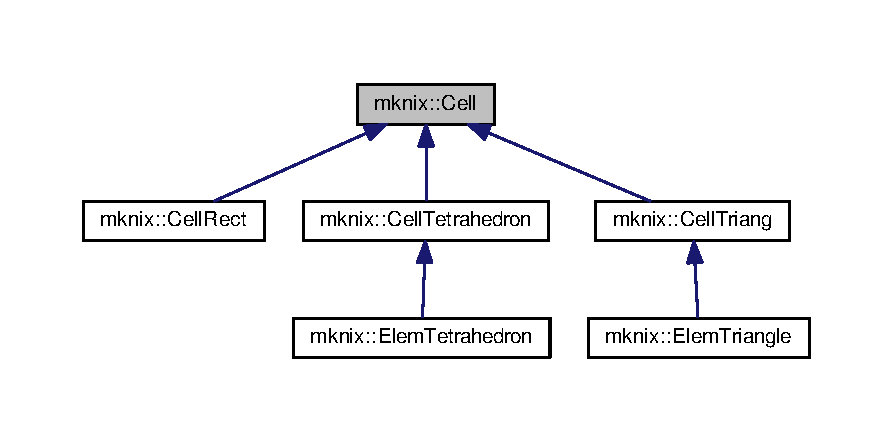
\includegraphics[width=350pt]{d4/d8c/classmknix_1_1_cell__inherit__graph}
\end{center}
\end{figure}


Collaboration diagram for mknix\+:\+:Cell\+:\nopagebreak
\begin{figure}[H]
\begin{center}
\leavevmode
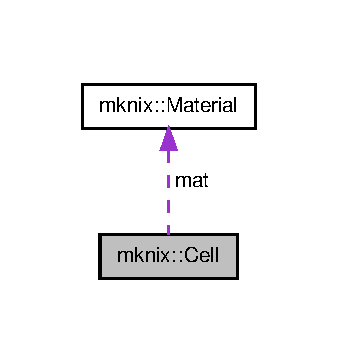
\includegraphics[width=163pt]{d0/d8c/classmknix_1_1_cell__coll__graph}
\end{center}
\end{figure}
\subsubsection*{Public Member Functions}
\begin{DoxyCompactItemize}
\item 
\hyperlink{classmknix_1_1_cell_a1c285cc4f38656550e8e2926058e8612}{Cell} ()
\item 
\hyperlink{classmknix_1_1_cell_ad0988ed8a4aac7c7440bee9413e1189f}{Cell} (\hyperlink{classmknix_1_1_material}{Material} \&, std\+::string, double, int)
\item 
virtual \hyperlink{classmknix_1_1_cell_ab4efc3f7c10212304dd776e7b58bb57b}{$\sim$\+Cell} ()
\item 
virtual void \hyperlink{classmknix_1_1_cell_a77d7851793538f99d8aa0ea664fa0fb7}{initialize} (std\+::vector$<$ \hyperlink{classmknix_1_1_node}{Node} $\ast$ $>$ \&)
\item 
virtual void \hyperlink{classmknix_1_1_cell_a6772f09fe6965faff4b53486b09f7235}{compute\+Shape\+Functions} ()
\item 
void \hyperlink{classmknix_1_1_cell_a675db1cafb39d5abab7b13994df21045}{compute\+Capacity\+Gauss\+Points} ()
\item 
void \hyperlink{classmknix_1_1_cell_a4d4af2c299e451b91a81819ccf5d6358}{assemble\+Capacity\+Gauss\+Points} (\hyperlink{classlmx_1_1_matrix}{lmx\+::\+Matrix}$<$ \hyperlink{namespacemknix_a16be4b246fbf2cceb141e3a179111020}{data\+\_\+type} $>$ \&)
\item 
void \hyperlink{classmknix_1_1_cell_a5d8c11ba58bbaa6f70d5dc2b530868e7}{compute\+Conductivity\+Gauss\+Points} ()
\item 
void \hyperlink{classmknix_1_1_cell_aae283c2a89beb517ed41b42bfdb19957}{assemble\+Conductivity\+Gauss\+Points} (\hyperlink{classlmx_1_1_matrix}{lmx\+::\+Matrix}$<$ \hyperlink{namespacemknix_a16be4b246fbf2cceb141e3a179111020}{data\+\_\+type} $>$ \&)
\item 
void \hyperlink{classmknix_1_1_cell_a98f6864613cfbac05b0f8ccbe067e743}{compute\+Qext\+Gauss\+Points} (\hyperlink{classmknix_1_1_load_thermal_body}{Load\+Thermal\+Body} $\ast$)
\item 
void \hyperlink{classmknix_1_1_cell_a130944ac8867e93ce882e7cc8c3555ca}{assemble\+Qext\+Gauss\+Points} (\hyperlink{classlmx_1_1_vector}{lmx\+::\+Vector}$<$ \hyperlink{namespacemknix_a16be4b246fbf2cceb141e3a179111020}{data\+\_\+type} $>$ \&)
\item 
void \hyperlink{classmknix_1_1_cell_a32a01eb5f854fc23353c0eb64b65e2da}{compute\+M\+Gauss\+Points} ()
\item 
void \hyperlink{classmknix_1_1_cell_a0b44063103766cd26b0411156c6d6004}{assemble\+M\+Gauss\+Points} (\hyperlink{classlmx_1_1_matrix}{lmx\+::\+Matrix}$<$ \hyperlink{namespacemknix_a16be4b246fbf2cceb141e3a179111020}{data\+\_\+type} $>$ \&)
\item 
void \hyperlink{classmknix_1_1_cell_a1c3123f613acd57332a6e84dc3736b86}{compute\+Fint\+Gauss\+Points} ()
\item 
void \hyperlink{classmknix_1_1_cell_a84014b9ed9c8a49c604f4ddb91b524fe}{compute\+N\+L\+Fint\+Gauss\+Points} ()
\item 
void \hyperlink{classmknix_1_1_cell_a1bf285b7dd7f06ece2f92e2b4389d6f5}{assemble\+Fint\+Gauss\+Points} (\hyperlink{classlmx_1_1_vector}{lmx\+::\+Vector}$<$ \hyperlink{namespacemknix_a16be4b246fbf2cceb141e3a179111020}{data\+\_\+type} $>$ \&)
\item 
void \hyperlink{classmknix_1_1_cell_a19b4ed719612fe2e0043d0cebcbe1537}{compute\+Fext\+Gauss\+Points} ()
\item 
void \hyperlink{classmknix_1_1_cell_a7c381e6cbcdb2478505645cad57a2c6e}{assemble\+Fext\+Gauss\+Points} (\hyperlink{classlmx_1_1_vector}{lmx\+::\+Vector}$<$ \hyperlink{namespacemknix_a16be4b246fbf2cceb141e3a179111020}{data\+\_\+type} $>$ \&)
\item 
void \hyperlink{classmknix_1_1_cell_a379600644881412c03608d3d32c36d49}{compute\+K\+Gauss\+Points} ()
\item 
void \hyperlink{classmknix_1_1_cell_a56231c1df8cd13f6b3f04356da6c2955}{compute\+N\+L\+K\+Gauss\+Points} ()
\item 
void \hyperlink{classmknix_1_1_cell_a8b703b97535562245382523c3702a054}{assemble\+K\+Gauss\+Points} (\hyperlink{classlmx_1_1_matrix}{lmx\+::\+Matrix}$<$ \hyperlink{namespacemknix_a16be4b246fbf2cceb141e3a179111020}{data\+\_\+type} $>$ \&)
\item 
void \hyperlink{classmknix_1_1_cell_a97fdd8bbf158f3b03b1af601177c2585}{assemble\+R\+Gauss\+Points} (\hyperlink{classlmx_1_1_vector}{lmx\+::\+Vector}$<$ \hyperlink{namespacemknix_a16be4b246fbf2cceb141e3a179111020}{data\+\_\+type} $>$ \&, int)
\item 
void \hyperlink{classmknix_1_1_cell_af65d528a607f3215d04449551db94dcd}{assemble\+N\+L\+R\+Gauss\+Points} (\hyperlink{classlmx_1_1_vector}{lmx\+::\+Vector}$<$ \hyperlink{namespacemknix_a16be4b246fbf2cceb141e3a179111020}{data\+\_\+type} $>$ \&, int)
\item 
double \hyperlink{classmknix_1_1_cell_a9aba982ff2a54738ec8b38446d333f8d}{calc\+Potential\+E\+Gauss\+Points} (const \hyperlink{classlmx_1_1_vector}{lmx\+::\+Vector}$<$ \hyperlink{namespacemknix_a16be4b246fbf2cceb141e3a179111020}{data\+\_\+type} $>$ \&)
\item 
double \hyperlink{classmknix_1_1_cell_aa0b40b9534a376333490fe73d921e552}{calc\+Kinetic\+E\+Gauss\+Points} (const \hyperlink{classlmx_1_1_vector}{lmx\+::\+Vector}$<$ \hyperlink{namespacemknix_a16be4b246fbf2cceb141e3a179111020}{data\+\_\+type} $>$ \&)
\item 
double \hyperlink{classmknix_1_1_cell_a1b59c56aa8983a27571c6809b03604c5}{calc\+Elastic\+E\+Gauss\+Points} ()
\item 
void \hyperlink{classmknix_1_1_cell_ab004ce4e03c629bd57a457e0a74f4d8b}{output\+Connectivity\+To\+File} (std\+::ofstream $\ast$)
\item 
virtual void \hyperlink{classmknix_1_1_cell_a345a938d058d10f60d6c302a715290de}{gnuplot\+Out} (std\+::ofstream \&, std\+::ofstream \&)=0
\item 
void \hyperlink{classmknix_1_1_cell_a6dd6795d452d5bd8ff26de1419baef31}{gnuplot\+Out\+Stress} (std\+::ofstream \&)
\end{DoxyCompactItemize}
\subsubsection*{Protected Attributes}
\begin{DoxyCompactItemize}
\item 
\hyperlink{classmknix_1_1_material}{Material} $\ast$ \hyperlink{classmknix_1_1_cell_a83ca13ff89196b3ab378d2a28820a08e}{mat}
\item 
std\+::string \hyperlink{classmknix_1_1_cell_ad637a730575145fbc61f884b2edac8f8}{formulation}
\item 
double \hyperlink{classmknix_1_1_cell_a79afef7ecbdfee69e687bb2e7559520b}{alpha}
\item 
int \hyperlink{classmknix_1_1_cell_a7d406d6e6f58c14da07387723986ae38}{n\+G\+Points}
\item 
std\+::vector$<$ \hyperlink{classmknix_1_1_gauss_point}{Gauss\+Point} $\ast$ $>$ \hyperlink{classmknix_1_1_cell_a980ae62ad7e6dda296257455ee173f86}{g\+Points}
\item 
std\+::vector$<$ \hyperlink{classmknix_1_1_gauss_point}{Gauss\+Point} $\ast$ $>$ \hyperlink{classmknix_1_1_cell_a45f0c5d52208a6166a71e05b190ece44}{g\+Points\+\_\+\+M\+C}
\item 
double \hyperlink{classmknix_1_1_cell_a4922bf34ba543606a8d9c5ca4847b589}{jacobian}
\item 
std\+::vector$<$ \hyperlink{classmknix_1_1_point}{Point} $\ast$ $>$ \hyperlink{classmknix_1_1_cell_a3b99f21386f177893f32289c95df4684}{body\+Points}
\item 
double \hyperlink{classmknix_1_1_cell_a7108fef12b0319adebeff93cab664314}{dc}
\end{DoxyCompactItemize}


\subsubsection{Detailed Description}
\begin{DoxyAuthor}{Author}
Daniel Iglesias 
\end{DoxyAuthor}


Definition at line 54 of file cell.\+h.



\subsubsection{Constructor \& Destructor Documentation}
\hypertarget{classmknix_1_1_cell_a1c285cc4f38656550e8e2926058e8612}{}\index{mknix\+::\+Cell@{mknix\+::\+Cell}!Cell@{Cell}}
\index{Cell@{Cell}!mknix\+::\+Cell@{mknix\+::\+Cell}}
\paragraph[{Cell}]{\setlength{\rightskip}{0pt plus 5cm}mknix\+::\+Cell\+::\+Cell (
\begin{DoxyParamCaption}
{}
\end{DoxyParamCaption}
)}\label{classmknix_1_1_cell_a1c285cc4f38656550e8e2926058e8612}


Definition at line 12 of file cell.\+cpp.

\hypertarget{classmknix_1_1_cell_ad0988ed8a4aac7c7440bee9413e1189f}{}\index{mknix\+::\+Cell@{mknix\+::\+Cell}!Cell@{Cell}}
\index{Cell@{Cell}!mknix\+::\+Cell@{mknix\+::\+Cell}}
\paragraph[{Cell}]{\setlength{\rightskip}{0pt plus 5cm}mknix\+::\+Cell\+::\+Cell (
\begin{DoxyParamCaption}
\item[{{\bf Material} \&}]{material\+\_\+in, }
\item[{std\+::string}]{formulation\+\_\+in, }
\item[{double}]{alpha\+\_\+in, }
\item[{int}]{n\+G\+Points\+\_\+in}
\end{DoxyParamCaption}
)}\label{classmknix_1_1_cell_ad0988ed8a4aac7c7440bee9413e1189f}


Definition at line 17 of file cell.\+cpp.

\hypertarget{classmknix_1_1_cell_ab4efc3f7c10212304dd776e7b58bb57b}{}\index{mknix\+::\+Cell@{mknix\+::\+Cell}!````~Cell@{$\sim$\+Cell}}
\index{````~Cell@{$\sim$\+Cell}!mknix\+::\+Cell@{mknix\+::\+Cell}}
\paragraph[{$\sim$\+Cell}]{\setlength{\rightskip}{0pt plus 5cm}mknix\+::\+Cell\+::$\sim$\+Cell (
\begin{DoxyParamCaption}
{}
\end{DoxyParamCaption}
)\hspace{0.3cm}{\ttfamily [virtual]}}\label{classmknix_1_1_cell_ab4efc3f7c10212304dd776e7b58bb57b}


Definition at line 29 of file cell.\+cpp.



\subsubsection{Member Function Documentation}
\hypertarget{classmknix_1_1_cell_a4d4af2c299e451b91a81819ccf5d6358}{}\index{mknix\+::\+Cell@{mknix\+::\+Cell}!assemble\+Capacity\+Gauss\+Points@{assemble\+Capacity\+Gauss\+Points}}
\index{assemble\+Capacity\+Gauss\+Points@{assemble\+Capacity\+Gauss\+Points}!mknix\+::\+Cell@{mknix\+::\+Cell}}
\paragraph[{assemble\+Capacity\+Gauss\+Points}]{\setlength{\rightskip}{0pt plus 5cm}void mknix\+::\+Cell\+::assemble\+Capacity\+Gauss\+Points (
\begin{DoxyParamCaption}
\item[{{\bf lmx\+::\+Matrix}$<$ {\bf data\+\_\+type} $>$ \&}]{global\+Capacity}
\end{DoxyParamCaption}
)}\label{classmknix_1_1_cell_a4d4af2c299e451b91a81819ccf5d6358}


Definition at line 87 of file cell.\+cpp.

\hypertarget{classmknix_1_1_cell_aae283c2a89beb517ed41b42bfdb19957}{}\index{mknix\+::\+Cell@{mknix\+::\+Cell}!assemble\+Conductivity\+Gauss\+Points@{assemble\+Conductivity\+Gauss\+Points}}
\index{assemble\+Conductivity\+Gauss\+Points@{assemble\+Conductivity\+Gauss\+Points}!mknix\+::\+Cell@{mknix\+::\+Cell}}
\paragraph[{assemble\+Conductivity\+Gauss\+Points}]{\setlength{\rightskip}{0pt plus 5cm}void mknix\+::\+Cell\+::assemble\+Conductivity\+Gauss\+Points (
\begin{DoxyParamCaption}
\item[{{\bf lmx\+::\+Matrix}$<$ {\bf data\+\_\+type} $>$ \&}]{global\+Conductivity}
\end{DoxyParamCaption}
)}\label{classmknix_1_1_cell_aae283c2a89beb517ed41b42bfdb19957}


Definition at line 102 of file cell.\+cpp.

\hypertarget{classmknix_1_1_cell_a7c381e6cbcdb2478505645cad57a2c6e}{}\index{mknix\+::\+Cell@{mknix\+::\+Cell}!assemble\+Fext\+Gauss\+Points@{assemble\+Fext\+Gauss\+Points}}
\index{assemble\+Fext\+Gauss\+Points@{assemble\+Fext\+Gauss\+Points}!mknix\+::\+Cell@{mknix\+::\+Cell}}
\paragraph[{assemble\+Fext\+Gauss\+Points}]{\setlength{\rightskip}{0pt plus 5cm}void mknix\+::\+Cell\+::assemble\+Fext\+Gauss\+Points (
\begin{DoxyParamCaption}
\item[{{\bf lmx\+::\+Vector}$<$ {\bf data\+\_\+type} $>$ \&}]{global\+Fext}
\end{DoxyParamCaption}
)}\label{classmknix_1_1_cell_a7c381e6cbcdb2478505645cad57a2c6e}


Definition at line 173 of file cell.\+cpp.

\hypertarget{classmknix_1_1_cell_a1bf285b7dd7f06ece2f92e2b4389d6f5}{}\index{mknix\+::\+Cell@{mknix\+::\+Cell}!assemble\+Fint\+Gauss\+Points@{assemble\+Fint\+Gauss\+Points}}
\index{assemble\+Fint\+Gauss\+Points@{assemble\+Fint\+Gauss\+Points}!mknix\+::\+Cell@{mknix\+::\+Cell}}
\paragraph[{assemble\+Fint\+Gauss\+Points}]{\setlength{\rightskip}{0pt plus 5cm}void mknix\+::\+Cell\+::assemble\+Fint\+Gauss\+Points (
\begin{DoxyParamCaption}
\item[{{\bf lmx\+::\+Vector}$<$ {\bf data\+\_\+type} $>$ \&}]{global\+Fint}
\end{DoxyParamCaption}
)}\label{classmknix_1_1_cell_a1bf285b7dd7f06ece2f92e2b4389d6f5}


Definition at line 157 of file cell.\+cpp.

\hypertarget{classmknix_1_1_cell_a8b703b97535562245382523c3702a054}{}\index{mknix\+::\+Cell@{mknix\+::\+Cell}!assemble\+K\+Gauss\+Points@{assemble\+K\+Gauss\+Points}}
\index{assemble\+K\+Gauss\+Points@{assemble\+K\+Gauss\+Points}!mknix\+::\+Cell@{mknix\+::\+Cell}}
\paragraph[{assemble\+K\+Gauss\+Points}]{\setlength{\rightskip}{0pt plus 5cm}void mknix\+::\+Cell\+::assemble\+K\+Gauss\+Points (
\begin{DoxyParamCaption}
\item[{{\bf lmx\+::\+Matrix}$<$ {\bf data\+\_\+type} $>$ \&}]{global\+Tangent}
\end{DoxyParamCaption}
)}\label{classmknix_1_1_cell_a8b703b97535562245382523c3702a054}


Definition at line 197 of file cell.\+cpp.

\hypertarget{classmknix_1_1_cell_a0b44063103766cd26b0411156c6d6004}{}\index{mknix\+::\+Cell@{mknix\+::\+Cell}!assemble\+M\+Gauss\+Points@{assemble\+M\+Gauss\+Points}}
\index{assemble\+M\+Gauss\+Points@{assemble\+M\+Gauss\+Points}!mknix\+::\+Cell@{mknix\+::\+Cell}}
\paragraph[{assemble\+M\+Gauss\+Points}]{\setlength{\rightskip}{0pt plus 5cm}void mknix\+::\+Cell\+::assemble\+M\+Gauss\+Points (
\begin{DoxyParamCaption}
\item[{{\bf lmx\+::\+Matrix}$<$ {\bf data\+\_\+type} $>$ \&}]{global\+Mass}
\end{DoxyParamCaption}
)}\label{classmknix_1_1_cell_a0b44063103766cd26b0411156c6d6004}


Definition at line 133 of file cell.\+cpp.

\hypertarget{classmknix_1_1_cell_af65d528a607f3215d04449551db94dcd}{}\index{mknix\+::\+Cell@{mknix\+::\+Cell}!assemble\+N\+L\+R\+Gauss\+Points@{assemble\+N\+L\+R\+Gauss\+Points}}
\index{assemble\+N\+L\+R\+Gauss\+Points@{assemble\+N\+L\+R\+Gauss\+Points}!mknix\+::\+Cell@{mknix\+::\+Cell}}
\paragraph[{assemble\+N\+L\+R\+Gauss\+Points}]{\setlength{\rightskip}{0pt plus 5cm}void mknix\+::\+Cell\+::assemble\+N\+L\+R\+Gauss\+Points (
\begin{DoxyParamCaption}
\item[{{\bf lmx\+::\+Vector}$<$ {\bf data\+\_\+type} $>$ \&}]{global\+Stress, }
\item[{int}]{first\+Node}
\end{DoxyParamCaption}
)}\label{classmknix_1_1_cell_af65d528a607f3215d04449551db94dcd}


Definition at line 216 of file cell.\+cpp.

\hypertarget{classmknix_1_1_cell_a130944ac8867e93ce882e7cc8c3555ca}{}\index{mknix\+::\+Cell@{mknix\+::\+Cell}!assemble\+Qext\+Gauss\+Points@{assemble\+Qext\+Gauss\+Points}}
\index{assemble\+Qext\+Gauss\+Points@{assemble\+Qext\+Gauss\+Points}!mknix\+::\+Cell@{mknix\+::\+Cell}}
\paragraph[{assemble\+Qext\+Gauss\+Points}]{\setlength{\rightskip}{0pt plus 5cm}void mknix\+::\+Cell\+::assemble\+Qext\+Gauss\+Points (
\begin{DoxyParamCaption}
\item[{{\bf lmx\+::\+Vector}$<$ {\bf data\+\_\+type} $>$ \&}]{global\+Qext}
\end{DoxyParamCaption}
)}\label{classmknix_1_1_cell_a130944ac8867e93ce882e7cc8c3555ca}


Definition at line 117 of file cell.\+cpp.

\hypertarget{classmknix_1_1_cell_a97fdd8bbf158f3b03b1af601177c2585}{}\index{mknix\+::\+Cell@{mknix\+::\+Cell}!assemble\+R\+Gauss\+Points@{assemble\+R\+Gauss\+Points}}
\index{assemble\+R\+Gauss\+Points@{assemble\+R\+Gauss\+Points}!mknix\+::\+Cell@{mknix\+::\+Cell}}
\paragraph[{assemble\+R\+Gauss\+Points}]{\setlength{\rightskip}{0pt plus 5cm}void mknix\+::\+Cell\+::assemble\+R\+Gauss\+Points (
\begin{DoxyParamCaption}
\item[{{\bf lmx\+::\+Vector}$<$ {\bf data\+\_\+type} $>$ \&}]{global\+Stress, }
\item[{int}]{first\+Node}
\end{DoxyParamCaption}
)}\label{classmknix_1_1_cell_a97fdd8bbf158f3b03b1af601177c2585}


Definition at line 205 of file cell.\+cpp.

\hypertarget{classmknix_1_1_cell_a1b59c56aa8983a27571c6809b03604c5}{}\index{mknix\+::\+Cell@{mknix\+::\+Cell}!calc\+Elastic\+E\+Gauss\+Points@{calc\+Elastic\+E\+Gauss\+Points}}
\index{calc\+Elastic\+E\+Gauss\+Points@{calc\+Elastic\+E\+Gauss\+Points}!mknix\+::\+Cell@{mknix\+::\+Cell}}
\paragraph[{calc\+Elastic\+E\+Gauss\+Points}]{\setlength{\rightskip}{0pt plus 5cm}double mknix\+::\+Cell\+::calc\+Elastic\+E\+Gauss\+Points (
\begin{DoxyParamCaption}
{}
\end{DoxyParamCaption}
)}\label{classmknix_1_1_cell_a1b59c56aa8983a27571c6809b03604c5}


Definition at line 249 of file cell.\+cpp.

\hypertarget{classmknix_1_1_cell_aa0b40b9534a376333490fe73d921e552}{}\index{mknix\+::\+Cell@{mknix\+::\+Cell}!calc\+Kinetic\+E\+Gauss\+Points@{calc\+Kinetic\+E\+Gauss\+Points}}
\index{calc\+Kinetic\+E\+Gauss\+Points@{calc\+Kinetic\+E\+Gauss\+Points}!mknix\+::\+Cell@{mknix\+::\+Cell}}
\paragraph[{calc\+Kinetic\+E\+Gauss\+Points}]{\setlength{\rightskip}{0pt plus 5cm}double mknix\+::\+Cell\+::calc\+Kinetic\+E\+Gauss\+Points (
\begin{DoxyParamCaption}
\item[{const {\bf lmx\+::\+Vector}$<$ {\bf data\+\_\+type} $>$ \&}]{qdot}
\end{DoxyParamCaption}
)}\label{classmknix_1_1_cell_aa0b40b9534a376333490fe73d921e552}


Definition at line 238 of file cell.\+cpp.

\hypertarget{classmknix_1_1_cell_a9aba982ff2a54738ec8b38446d333f8d}{}\index{mknix\+::\+Cell@{mknix\+::\+Cell}!calc\+Potential\+E\+Gauss\+Points@{calc\+Potential\+E\+Gauss\+Points}}
\index{calc\+Potential\+E\+Gauss\+Points@{calc\+Potential\+E\+Gauss\+Points}!mknix\+::\+Cell@{mknix\+::\+Cell}}
\paragraph[{calc\+Potential\+E\+Gauss\+Points}]{\setlength{\rightskip}{0pt plus 5cm}double mknix\+::\+Cell\+::calc\+Potential\+E\+Gauss\+Points (
\begin{DoxyParamCaption}
\item[{const {\bf lmx\+::\+Vector}$<$ {\bf data\+\_\+type} $>$ \&}]{q}
\end{DoxyParamCaption}
)}\label{classmknix_1_1_cell_a9aba982ff2a54738ec8b38446d333f8d}


Definition at line 227 of file cell.\+cpp.

\hypertarget{classmknix_1_1_cell_a675db1cafb39d5abab7b13994df21045}{}\index{mknix\+::\+Cell@{mknix\+::\+Cell}!compute\+Capacity\+Gauss\+Points@{compute\+Capacity\+Gauss\+Points}}
\index{compute\+Capacity\+Gauss\+Points@{compute\+Capacity\+Gauss\+Points}!mknix\+::\+Cell@{mknix\+::\+Cell}}
\paragraph[{compute\+Capacity\+Gauss\+Points}]{\setlength{\rightskip}{0pt plus 5cm}void mknix\+::\+Cell\+::compute\+Capacity\+Gauss\+Points (
\begin{DoxyParamCaption}
{}
\end{DoxyParamCaption}
)}\label{classmknix_1_1_cell_a675db1cafb39d5abab7b13994df21045}


Definition at line 80 of file cell.\+cpp.

\hypertarget{classmknix_1_1_cell_a5d8c11ba58bbaa6f70d5dc2b530868e7}{}\index{mknix\+::\+Cell@{mknix\+::\+Cell}!compute\+Conductivity\+Gauss\+Points@{compute\+Conductivity\+Gauss\+Points}}
\index{compute\+Conductivity\+Gauss\+Points@{compute\+Conductivity\+Gauss\+Points}!mknix\+::\+Cell@{mknix\+::\+Cell}}
\paragraph[{compute\+Conductivity\+Gauss\+Points}]{\setlength{\rightskip}{0pt plus 5cm}void mknix\+::\+Cell\+::compute\+Conductivity\+Gauss\+Points (
\begin{DoxyParamCaption}
{}
\end{DoxyParamCaption}
)}\label{classmknix_1_1_cell_a5d8c11ba58bbaa6f70d5dc2b530868e7}


Definition at line 95 of file cell.\+cpp.

\hypertarget{classmknix_1_1_cell_a19b4ed719612fe2e0043d0cebcbe1537}{}\index{mknix\+::\+Cell@{mknix\+::\+Cell}!compute\+Fext\+Gauss\+Points@{compute\+Fext\+Gauss\+Points}}
\index{compute\+Fext\+Gauss\+Points@{compute\+Fext\+Gauss\+Points}!mknix\+::\+Cell@{mknix\+::\+Cell}}
\paragraph[{compute\+Fext\+Gauss\+Points}]{\setlength{\rightskip}{0pt plus 5cm}void mknix\+::\+Cell\+::compute\+Fext\+Gauss\+Points (
\begin{DoxyParamCaption}
{}
\end{DoxyParamCaption}
)}\label{classmknix_1_1_cell_a19b4ed719612fe2e0043d0cebcbe1537}


Definition at line 165 of file cell.\+cpp.

\hypertarget{classmknix_1_1_cell_a1c3123f613acd57332a6e84dc3736b86}{}\index{mknix\+::\+Cell@{mknix\+::\+Cell}!compute\+Fint\+Gauss\+Points@{compute\+Fint\+Gauss\+Points}}
\index{compute\+Fint\+Gauss\+Points@{compute\+Fint\+Gauss\+Points}!mknix\+::\+Cell@{mknix\+::\+Cell}}
\paragraph[{compute\+Fint\+Gauss\+Points}]{\setlength{\rightskip}{0pt plus 5cm}void mknix\+::\+Cell\+::compute\+Fint\+Gauss\+Points (
\begin{DoxyParamCaption}
{}
\end{DoxyParamCaption}
)}\label{classmknix_1_1_cell_a1c3123f613acd57332a6e84dc3736b86}


Definition at line 141 of file cell.\+cpp.

\hypertarget{classmknix_1_1_cell_a379600644881412c03608d3d32c36d49}{}\index{mknix\+::\+Cell@{mknix\+::\+Cell}!compute\+K\+Gauss\+Points@{compute\+K\+Gauss\+Points}}
\index{compute\+K\+Gauss\+Points@{compute\+K\+Gauss\+Points}!mknix\+::\+Cell@{mknix\+::\+Cell}}
\paragraph[{compute\+K\+Gauss\+Points}]{\setlength{\rightskip}{0pt plus 5cm}void mknix\+::\+Cell\+::compute\+K\+Gauss\+Points (
\begin{DoxyParamCaption}
{}
\end{DoxyParamCaption}
)}\label{classmknix_1_1_cell_a379600644881412c03608d3d32c36d49}


Definition at line 181 of file cell.\+cpp.

\hypertarget{classmknix_1_1_cell_a32a01eb5f854fc23353c0eb64b65e2da}{}\index{mknix\+::\+Cell@{mknix\+::\+Cell}!compute\+M\+Gauss\+Points@{compute\+M\+Gauss\+Points}}
\index{compute\+M\+Gauss\+Points@{compute\+M\+Gauss\+Points}!mknix\+::\+Cell@{mknix\+::\+Cell}}
\paragraph[{compute\+M\+Gauss\+Points}]{\setlength{\rightskip}{0pt plus 5cm}void mknix\+::\+Cell\+::compute\+M\+Gauss\+Points (
\begin{DoxyParamCaption}
{}
\end{DoxyParamCaption}
)}\label{classmknix_1_1_cell_a32a01eb5f854fc23353c0eb64b65e2da}


Definition at line 125 of file cell.\+cpp.

\hypertarget{classmknix_1_1_cell_a84014b9ed9c8a49c604f4ddb91b524fe}{}\index{mknix\+::\+Cell@{mknix\+::\+Cell}!compute\+N\+L\+Fint\+Gauss\+Points@{compute\+N\+L\+Fint\+Gauss\+Points}}
\index{compute\+N\+L\+Fint\+Gauss\+Points@{compute\+N\+L\+Fint\+Gauss\+Points}!mknix\+::\+Cell@{mknix\+::\+Cell}}
\paragraph[{compute\+N\+L\+Fint\+Gauss\+Points}]{\setlength{\rightskip}{0pt plus 5cm}void mknix\+::\+Cell\+::compute\+N\+L\+Fint\+Gauss\+Points (
\begin{DoxyParamCaption}
{}
\end{DoxyParamCaption}
)}\label{classmknix_1_1_cell_a84014b9ed9c8a49c604f4ddb91b524fe}


Definition at line 149 of file cell.\+cpp.

\hypertarget{classmknix_1_1_cell_a56231c1df8cd13f6b3f04356da6c2955}{}\index{mknix\+::\+Cell@{mknix\+::\+Cell}!compute\+N\+L\+K\+Gauss\+Points@{compute\+N\+L\+K\+Gauss\+Points}}
\index{compute\+N\+L\+K\+Gauss\+Points@{compute\+N\+L\+K\+Gauss\+Points}!mknix\+::\+Cell@{mknix\+::\+Cell}}
\paragraph[{compute\+N\+L\+K\+Gauss\+Points}]{\setlength{\rightskip}{0pt plus 5cm}void mknix\+::\+Cell\+::compute\+N\+L\+K\+Gauss\+Points (
\begin{DoxyParamCaption}
{}
\end{DoxyParamCaption}
)}\label{classmknix_1_1_cell_a56231c1df8cd13f6b3f04356da6c2955}


Definition at line 189 of file cell.\+cpp.

\hypertarget{classmknix_1_1_cell_a98f6864613cfbac05b0f8ccbe067e743}{}\index{mknix\+::\+Cell@{mknix\+::\+Cell}!compute\+Qext\+Gauss\+Points@{compute\+Qext\+Gauss\+Points}}
\index{compute\+Qext\+Gauss\+Points@{compute\+Qext\+Gauss\+Points}!mknix\+::\+Cell@{mknix\+::\+Cell}}
\paragraph[{compute\+Qext\+Gauss\+Points}]{\setlength{\rightskip}{0pt plus 5cm}void mknix\+::\+Cell\+::compute\+Qext\+Gauss\+Points (
\begin{DoxyParamCaption}
\item[{{\bf Load\+Thermal\+Body} $\ast$}]{load\+Thermal\+Body\+\_\+in}
\end{DoxyParamCaption}
)}\label{classmknix_1_1_cell_a98f6864613cfbac05b0f8ccbe067e743}


Definition at line 110 of file cell.\+cpp.

\hypertarget{classmknix_1_1_cell_a6772f09fe6965faff4b53486b09f7235}{}\index{mknix\+::\+Cell@{mknix\+::\+Cell}!compute\+Shape\+Functions@{compute\+Shape\+Functions}}
\index{compute\+Shape\+Functions@{compute\+Shape\+Functions}!mknix\+::\+Cell@{mknix\+::\+Cell}}
\paragraph[{compute\+Shape\+Functions}]{\setlength{\rightskip}{0pt plus 5cm}void mknix\+::\+Cell\+::compute\+Shape\+Functions (
\begin{DoxyParamCaption}
{}
\end{DoxyParamCaption}
)\hspace{0.3cm}{\ttfamily [virtual]}}\label{classmknix_1_1_cell_a6772f09fe6965faff4b53486b09f7235}


Reimplemented in \hyperlink{classmknix_1_1_elem_tetrahedron_a09d199d493dd9642da2ccb7190306b18}{mknix\+::\+Elem\+Tetrahedron}, and \hyperlink{classmknix_1_1_elem_triangle_a6d97673aa922fca3c84ae23255b76223}{mknix\+::\+Elem\+Triangle}.



Definition at line 68 of file cell.\+cpp.

\hypertarget{classmknix_1_1_cell_a345a938d058d10f60d6c302a715290de}{}\index{mknix\+::\+Cell@{mknix\+::\+Cell}!gnuplot\+Out@{gnuplot\+Out}}
\index{gnuplot\+Out@{gnuplot\+Out}!mknix\+::\+Cell@{mknix\+::\+Cell}}
\paragraph[{gnuplot\+Out}]{\setlength{\rightskip}{0pt plus 5cm}virtual void mknix\+::\+Cell\+::gnuplot\+Out (
\begin{DoxyParamCaption}
\item[{std\+::ofstream \&}]{, }
\item[{std\+::ofstream \&}]{}
\end{DoxyParamCaption}
)\hspace{0.3cm}{\ttfamily [pure virtual]}}\label{classmknix_1_1_cell_a345a938d058d10f60d6c302a715290de}


Implemented in \hyperlink{classmknix_1_1_cell_rect_aff6050da82b250a264f856743b0225e0}{mknix\+::\+Cell\+Rect}, \hyperlink{classmknix_1_1_cell_triang_a374f66822e2e37d94a2cfe09c5173e8a}{mknix\+::\+Cell\+Triang}, and \hyperlink{classmknix_1_1_cell_tetrahedron_aba4f93f294a8ceea377cc2feb44f56db}{mknix\+::\+Cell\+Tetrahedron}.

\hypertarget{classmknix_1_1_cell_a6dd6795d452d5bd8ff26de1419baef31}{}\index{mknix\+::\+Cell@{mknix\+::\+Cell}!gnuplot\+Out\+Stress@{gnuplot\+Out\+Stress}}
\index{gnuplot\+Out\+Stress@{gnuplot\+Out\+Stress}!mknix\+::\+Cell@{mknix\+::\+Cell}}
\paragraph[{gnuplot\+Out\+Stress}]{\setlength{\rightskip}{0pt plus 5cm}void mknix\+::\+Cell\+::gnuplot\+Out\+Stress (
\begin{DoxyParamCaption}
\item[{std\+::ofstream \&}]{gptension}
\end{DoxyParamCaption}
)}\label{classmknix_1_1_cell_a6dd6795d452d5bd8ff26de1419baef31}


Definition at line 270 of file cell.\+cpp.

\hypertarget{classmknix_1_1_cell_a77d7851793538f99d8aa0ea664fa0fb7}{}\index{mknix\+::\+Cell@{mknix\+::\+Cell}!initialize@{initialize}}
\index{initialize@{initialize}!mknix\+::\+Cell@{mknix\+::\+Cell}}
\paragraph[{initialize}]{\setlength{\rightskip}{0pt plus 5cm}void mknix\+::\+Cell\+::initialize (
\begin{DoxyParamCaption}
\item[{std\+::vector$<$ {\bf Node} $\ast$ $>$ \&}]{nodes\+\_\+in}
\end{DoxyParamCaption}
)\hspace{0.3cm}{\ttfamily [virtual]}}\label{classmknix_1_1_cell_a77d7851793538f99d8aa0ea664fa0fb7}


Reimplemented in \hyperlink{classmknix_1_1_cell_rect_a599daac72085b935a90afe8ffcecdd20}{mknix\+::\+Cell\+Rect}, \hyperlink{classmknix_1_1_elem_tetrahedron_a1f42683d35b87bfd4ddd4e83824d040d}{mknix\+::\+Elem\+Tetrahedron}, and \hyperlink{classmknix_1_1_elem_triangle_a5ddf93646f4b35632801fd28bc8e14a2}{mknix\+::\+Elem\+Triangle}.



Definition at line 42 of file cell.\+cpp.

\hypertarget{classmknix_1_1_cell_ab004ce4e03c629bd57a457e0a74f4d8b}{}\index{mknix\+::\+Cell@{mknix\+::\+Cell}!output\+Connectivity\+To\+File@{output\+Connectivity\+To\+File}}
\index{output\+Connectivity\+To\+File@{output\+Connectivity\+To\+File}!mknix\+::\+Cell@{mknix\+::\+Cell}}
\paragraph[{output\+Connectivity\+To\+File}]{\setlength{\rightskip}{0pt plus 5cm}void mknix\+::\+Cell\+::output\+Connectivity\+To\+File (
\begin{DoxyParamCaption}
\item[{std\+::ofstream $\ast$}]{outfile}
\end{DoxyParamCaption}
)}\label{classmknix_1_1_cell_ab004ce4e03c629bd57a457e0a74f4d8b}


Definition at line 260 of file cell.\+cpp.



\subsubsection{Member Data Documentation}
\hypertarget{classmknix_1_1_cell_a79afef7ecbdfee69e687bb2e7559520b}{}\index{mknix\+::\+Cell@{mknix\+::\+Cell}!alpha@{alpha}}
\index{alpha@{alpha}!mknix\+::\+Cell@{mknix\+::\+Cell}}
\paragraph[{alpha}]{\setlength{\rightskip}{0pt plus 5cm}double mknix\+::\+Cell\+::alpha\hspace{0.3cm}{\ttfamily [protected]}}\label{classmknix_1_1_cell_a79afef7ecbdfee69e687bb2e7559520b}


Definition at line 118 of file cell.\+h.

\hypertarget{classmknix_1_1_cell_a3b99f21386f177893f32289c95df4684}{}\index{mknix\+::\+Cell@{mknix\+::\+Cell}!body\+Points@{body\+Points}}
\index{body\+Points@{body\+Points}!mknix\+::\+Cell@{mknix\+::\+Cell}}
\paragraph[{body\+Points}]{\setlength{\rightskip}{0pt plus 5cm}std\+::vector$<$ {\bf Point}$\ast$ $>$ mknix\+::\+Cell\+::body\+Points\hspace{0.3cm}{\ttfamily [protected]}}\label{classmknix_1_1_cell_a3b99f21386f177893f32289c95df4684}


Definition at line 123 of file cell.\+h.

\hypertarget{classmknix_1_1_cell_a7108fef12b0319adebeff93cab664314}{}\index{mknix\+::\+Cell@{mknix\+::\+Cell}!dc@{dc}}
\index{dc@{dc}!mknix\+::\+Cell@{mknix\+::\+Cell}}
\paragraph[{dc}]{\setlength{\rightskip}{0pt plus 5cm}double mknix\+::\+Cell\+::dc\hspace{0.3cm}{\ttfamily [protected]}}\label{classmknix_1_1_cell_a7108fef12b0319adebeff93cab664314}


Definition at line 124 of file cell.\+h.

\hypertarget{classmknix_1_1_cell_ad637a730575145fbc61f884b2edac8f8}{}\index{mknix\+::\+Cell@{mknix\+::\+Cell}!formulation@{formulation}}
\index{formulation@{formulation}!mknix\+::\+Cell@{mknix\+::\+Cell}}
\paragraph[{formulation}]{\setlength{\rightskip}{0pt plus 5cm}std\+::string mknix\+::\+Cell\+::formulation\hspace{0.3cm}{\ttfamily [protected]}}\label{classmknix_1_1_cell_ad637a730575145fbc61f884b2edac8f8}


Definition at line 117 of file cell.\+h.

\hypertarget{classmknix_1_1_cell_a980ae62ad7e6dda296257455ee173f86}{}\index{mknix\+::\+Cell@{mknix\+::\+Cell}!g\+Points@{g\+Points}}
\index{g\+Points@{g\+Points}!mknix\+::\+Cell@{mknix\+::\+Cell}}
\paragraph[{g\+Points}]{\setlength{\rightskip}{0pt plus 5cm}std\+::vector$<${\bf Gauss\+Point}$\ast$$>$ mknix\+::\+Cell\+::g\+Points\hspace{0.3cm}{\ttfamily [protected]}}\label{classmknix_1_1_cell_a980ae62ad7e6dda296257455ee173f86}


Definition at line 120 of file cell.\+h.

\hypertarget{classmknix_1_1_cell_a45f0c5d52208a6166a71e05b190ece44}{}\index{mknix\+::\+Cell@{mknix\+::\+Cell}!g\+Points\+\_\+\+M\+C@{g\+Points\+\_\+\+M\+C}}
\index{g\+Points\+\_\+\+M\+C@{g\+Points\+\_\+\+M\+C}!mknix\+::\+Cell@{mknix\+::\+Cell}}
\paragraph[{g\+Points\+\_\+\+M\+C}]{\setlength{\rightskip}{0pt plus 5cm}std\+::vector$<${\bf Gauss\+Point}$\ast$$>$ mknix\+::\+Cell\+::g\+Points\+\_\+\+M\+C\hspace{0.3cm}{\ttfamily [protected]}}\label{classmknix_1_1_cell_a45f0c5d52208a6166a71e05b190ece44}


Definition at line 121 of file cell.\+h.

\hypertarget{classmknix_1_1_cell_a4922bf34ba543606a8d9c5ca4847b589}{}\index{mknix\+::\+Cell@{mknix\+::\+Cell}!jacobian@{jacobian}}
\index{jacobian@{jacobian}!mknix\+::\+Cell@{mknix\+::\+Cell}}
\paragraph[{jacobian}]{\setlength{\rightskip}{0pt plus 5cm}double mknix\+::\+Cell\+::jacobian\hspace{0.3cm}{\ttfamily [protected]}}\label{classmknix_1_1_cell_a4922bf34ba543606a8d9c5ca4847b589}


Definition at line 122 of file cell.\+h.

\hypertarget{classmknix_1_1_cell_a83ca13ff89196b3ab378d2a28820a08e}{}\index{mknix\+::\+Cell@{mknix\+::\+Cell}!mat@{mat}}
\index{mat@{mat}!mknix\+::\+Cell@{mknix\+::\+Cell}}
\paragraph[{mat}]{\setlength{\rightskip}{0pt plus 5cm}{\bf Material}$\ast$ mknix\+::\+Cell\+::mat\hspace{0.3cm}{\ttfamily [protected]}}\label{classmknix_1_1_cell_a83ca13ff89196b3ab378d2a28820a08e}


Definition at line 116 of file cell.\+h.

\hypertarget{classmknix_1_1_cell_a7d406d6e6f58c14da07387723986ae38}{}\index{mknix\+::\+Cell@{mknix\+::\+Cell}!n\+G\+Points@{n\+G\+Points}}
\index{n\+G\+Points@{n\+G\+Points}!mknix\+::\+Cell@{mknix\+::\+Cell}}
\paragraph[{n\+G\+Points}]{\setlength{\rightskip}{0pt plus 5cm}int mknix\+::\+Cell\+::n\+G\+Points\hspace{0.3cm}{\ttfamily [protected]}}\label{classmknix_1_1_cell_a7d406d6e6f58c14da07387723986ae38}
number of Gauss Points 

Definition at line 119 of file cell.\+h.



The documentation for this class was generated from the following files\+:\begin{DoxyCompactItemize}
\item 
\hyperlink{cell_8h}{cell.\+h}\item 
\hyperlink{cell_8cpp}{cell.\+cpp}\end{DoxyCompactItemize}

\hypertarget{classmknix_1_1_cell_rect}{\subsection{mknix\-:\-:Cell\-Rect Class Reference}
\label{classmknix_1_1_cell_rect}\index{mknix\-::\-Cell\-Rect@{mknix\-::\-Cell\-Rect}}
}


{\ttfamily \#include $<$cellrect.\-h$>$}



Inheritance diagram for mknix\-:\-:Cell\-Rect\-:\nopagebreak
\begin{figure}[H]
\begin{center}
\leavevmode
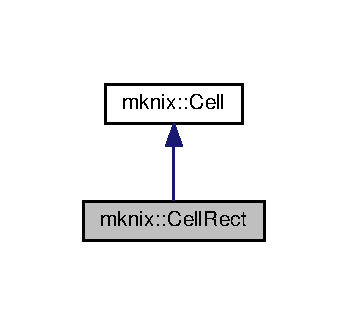
\includegraphics[width=166pt]{d4/dac/classmknix_1_1_cell_rect__inherit__graph}
\end{center}
\end{figure}


Collaboration diagram for mknix\-:\-:Cell\-Rect\-:\nopagebreak
\begin{figure}[H]
\begin{center}
\leavevmode
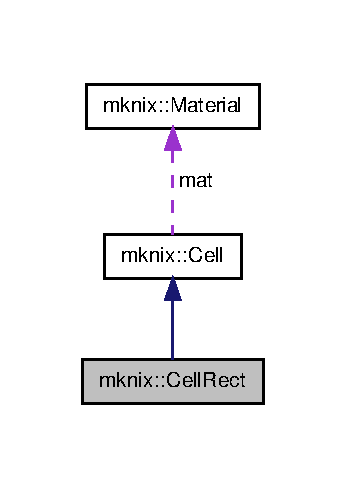
\includegraphics[width=166pt]{d3/db0/classmknix_1_1_cell_rect__coll__graph}
\end{center}
\end{figure}
\subsubsection*{Public Member Functions}
\begin{DoxyCompactItemize}
\item 
\hyperlink{classmknix_1_1_cell_rect_a7cc280eb130683f2b8d77ce04d3f7e84}{Cell\-Rect} ()
\item 
\hyperlink{classmknix_1_1_cell_rect_a5242df2938d1f9f60cd089c5309fa1c2}{Cell\-Rect} (\hyperlink{classmknix_1_1_material}{Material} \&, std\-::string, double, int, double, double, double, double, double, double, double, double, double, double, double, double, double, double)
\item 
\hyperlink{classmknix_1_1_cell_rect_a16a49a17652e7941217e1089bb243a6f}{Cell\-Rect} (\hyperlink{classmknix_1_1_material}{Material} \&, std\-::string, double, int, double, double, double, double, double, double, double, double, double, double, double, double, double, double, double, double, double, double, double, double, double, double, double, double, double, double, double, double, double, double, double, double, double)
\item 
\hyperlink{classmknix_1_1_cell_rect_a966a8afa0dee4990f8231cb7e32d33ee}{$\sim$\-Cell\-Rect} ()
\item 
void \hyperlink{classmknix_1_1_cell_rect_a599daac72085b935a90afe8ffcecdd20}{initialize} (std\-::vector$<$ \hyperlink{classmknix_1_1_node}{Node} $\ast$ $>$ \&)
\item 
void \hyperlink{classmknix_1_1_cell_rect_aff6050da82b250a264f856743b0225e0}{gnuplot\-Out} (std\-::ofstream \&, std\-::ofstream \&)
\end{DoxyCompactItemize}
\subsubsection*{Additional Inherited Members}


\subsubsection{Detailed Description}
\begin{DoxyAuthor}{Author}
Daniel Iglesias 
\end{DoxyAuthor}


\subsubsection{Constructor \& Destructor Documentation}
\hypertarget{classmknix_1_1_cell_rect_a7cc280eb130683f2b8d77ce04d3f7e84}{\index{mknix\-::\-Cell\-Rect@{mknix\-::\-Cell\-Rect}!Cell\-Rect@{Cell\-Rect}}
\index{Cell\-Rect@{Cell\-Rect}!mknix::CellRect@{mknix\-::\-Cell\-Rect}}
\paragraph[{Cell\-Rect}]{\setlength{\rightskip}{0pt plus 5cm}mknix\-::\-Cell\-Rect\-::\-Cell\-Rect (
\begin{DoxyParamCaption}
{}
\end{DoxyParamCaption}
)}}\label{classmknix_1_1_cell_rect_a7cc280eb130683f2b8d77ce04d3f7e84}
\hypertarget{classmknix_1_1_cell_rect_a5242df2938d1f9f60cd089c5309fa1c2}{\index{mknix\-::\-Cell\-Rect@{mknix\-::\-Cell\-Rect}!Cell\-Rect@{Cell\-Rect}}
\index{Cell\-Rect@{Cell\-Rect}!mknix::CellRect@{mknix\-::\-Cell\-Rect}}
\paragraph[{Cell\-Rect}]{\setlength{\rightskip}{0pt plus 5cm}mknix\-::\-Cell\-Rect\-::\-Cell\-Rect (
\begin{DoxyParamCaption}
\item[{{\bf Material} \&}]{material\-\_\-in, }
\item[{std\-::string}]{formulation\-\_\-in, }
\item[{double}]{alpha\-\_\-in, }
\item[{int}]{n\-G\-Points\-\_\-in, }
\item[{double}]{x1\-\_\-in, }
\item[{double}]{y1\-\_\-in, }
\item[{double}]{x2\-\_\-in, }
\item[{double}]{y2\-\_\-in, }
\item[{double}]{x3\-\_\-in, }
\item[{double}]{y3\-\_\-in, }
\item[{double}]{x4\-\_\-in, }
\item[{double}]{y4\-\_\-in, }
\item[{double}]{dcx\-\_\-in, }
\item[{double}]{dcy\-\_\-in, }
\item[{double}]{min\-X\-\_\-in, }
\item[{double}]{min\-Y\-\_\-in, }
\item[{double}]{max\-X\-\_\-in, }
\item[{double}]{max\-Y\-\_\-in}
\end{DoxyParamCaption}
)}}\label{classmknix_1_1_cell_rect_a5242df2938d1f9f60cd089c5309fa1c2}
\hypertarget{classmknix_1_1_cell_rect_a16a49a17652e7941217e1089bb243a6f}{\index{mknix\-::\-Cell\-Rect@{mknix\-::\-Cell\-Rect}!Cell\-Rect@{Cell\-Rect}}
\index{Cell\-Rect@{Cell\-Rect}!mknix::CellRect@{mknix\-::\-Cell\-Rect}}
\paragraph[{Cell\-Rect}]{\setlength{\rightskip}{0pt plus 5cm}mknix\-::\-Cell\-Rect\-::\-Cell\-Rect (
\begin{DoxyParamCaption}
\item[{{\bf Material} \&}]{material\-\_\-in, }
\item[{std\-::string}]{formulation\-\_\-in, }
\item[{double}]{alpha\-\_\-in, }
\item[{int}]{n\-G\-Points\-\_\-in, }
\item[{double}]{x1\-\_\-in, }
\item[{double}]{y1\-\_\-in, }
\item[{double}]{z1\-\_\-in, }
\item[{double}]{x2\-\_\-in, }
\item[{double}]{y2\-\_\-in, }
\item[{double}]{z2\-\_\-in, }
\item[{double}]{x3\-\_\-in, }
\item[{double}]{y3\-\_\-in, }
\item[{double}]{z3\-\_\-in, }
\item[{double}]{x4\-\_\-in, }
\item[{double}]{y4\-\_\-in, }
\item[{double}]{z4\-\_\-in, }
\item[{double}]{x5\-\_\-in, }
\item[{double}]{y5\-\_\-in, }
\item[{double}]{z5\-\_\-in, }
\item[{double}]{x6\-\_\-in, }
\item[{double}]{y6\-\_\-in, }
\item[{double}]{z6\-\_\-in, }
\item[{double}]{x7\-\_\-in, }
\item[{double}]{y7\-\_\-in, }
\item[{double}]{z7\-\_\-in, }
\item[{double}]{x8\-\_\-in, }
\item[{double}]{y8\-\_\-in, }
\item[{double}]{z8\-\_\-in, }
\item[{double}]{dcx\-\_\-in, }
\item[{double}]{dcy\-\_\-in, }
\item[{double}]{dcz\-\_\-in, }
\item[{double}]{min\-X\-\_\-in, }
\item[{double}]{min\-Y\-\_\-in, }
\item[{double}]{min\-Z\-\_\-in, }
\item[{double}]{max\-X\-\_\-in, }
\item[{double}]{max\-Y\-\_\-in, }
\item[{double}]{max\-Z\-\_\-in}
\end{DoxyParamCaption}
)}}\label{classmknix_1_1_cell_rect_a16a49a17652e7941217e1089bb243a6f}
\hypertarget{classmknix_1_1_cell_rect_a966a8afa0dee4990f8231cb7e32d33ee}{\index{mknix\-::\-Cell\-Rect@{mknix\-::\-Cell\-Rect}!$\sim$\-Cell\-Rect@{$\sim$\-Cell\-Rect}}
\index{$\sim$\-Cell\-Rect@{$\sim$\-Cell\-Rect}!mknix::CellRect@{mknix\-::\-Cell\-Rect}}
\paragraph[{$\sim$\-Cell\-Rect}]{\setlength{\rightskip}{0pt plus 5cm}mknix\-::\-Cell\-Rect\-::$\sim$\-Cell\-Rect (
\begin{DoxyParamCaption}
{}
\end{DoxyParamCaption}
)}}\label{classmknix_1_1_cell_rect_a966a8afa0dee4990f8231cb7e32d33ee}


\subsubsection{Member Function Documentation}
\hypertarget{classmknix_1_1_cell_rect_aff6050da82b250a264f856743b0225e0}{\index{mknix\-::\-Cell\-Rect@{mknix\-::\-Cell\-Rect}!gnuplot\-Out@{gnuplot\-Out}}
\index{gnuplot\-Out@{gnuplot\-Out}!mknix::CellRect@{mknix\-::\-Cell\-Rect}}
\paragraph[{gnuplot\-Out}]{\setlength{\rightskip}{0pt plus 5cm}void mknix\-::\-Cell\-Rect\-::gnuplot\-Out (
\begin{DoxyParamCaption}
\item[{std\-::ofstream \&}]{data, }
\item[{std\-::ofstream \&}]{gpdata}
\end{DoxyParamCaption}
)\hspace{0.3cm}{\ttfamily [virtual]}}}\label{classmknix_1_1_cell_rect_aff6050da82b250a264f856743b0225e0}


Implements \hyperlink{classmknix_1_1_cell_a345a938d058d10f60d6c302a715290de}{mknix\-::\-Cell}.

\hypertarget{classmknix_1_1_cell_rect_a599daac72085b935a90afe8ffcecdd20}{\index{mknix\-::\-Cell\-Rect@{mknix\-::\-Cell\-Rect}!initialize@{initialize}}
\index{initialize@{initialize}!mknix::CellRect@{mknix\-::\-Cell\-Rect}}
\paragraph[{initialize}]{\setlength{\rightskip}{0pt plus 5cm}void mknix\-::\-Cell\-Rect\-::initialize (
\begin{DoxyParamCaption}
\item[{std\-::vector$<$ {\bf Node} $\ast$ $>$ \&}]{nodes\-\_\-in}
\end{DoxyParamCaption}
)\hspace{0.3cm}{\ttfamily [virtual]}}}\label{classmknix_1_1_cell_rect_a599daac72085b935a90afe8ffcecdd20}


Reimplemented from \hyperlink{classmknix_1_1_cell_a77d7851793538f99d8aa0ea664fa0fb7}{mknix\-::\-Cell}.



The documentation for this class was generated from the following files\-:\begin{DoxyCompactItemize}
\item 
\hyperlink{cellrect_8h}{cellrect.\-h}\item 
\hyperlink{cellrect_8cpp}{cellrect.\-cpp}\end{DoxyCompactItemize}

\hypertarget{classmknix_1_1_cell_tetrahedron}{}\subsection{mknix\+:\+:Cell\+Tetrahedron Class Reference}
\label{classmknix_1_1_cell_tetrahedron}\index{mknix\+::\+Cell\+Tetrahedron@{mknix\+::\+Cell\+Tetrahedron}}


{\ttfamily \#include $<$celltetrahedron.\+h$>$}



Inheritance diagram for mknix\+:\+:Cell\+Tetrahedron\+:\nopagebreak
\begin{figure}[H]
\begin{center}
\leavevmode
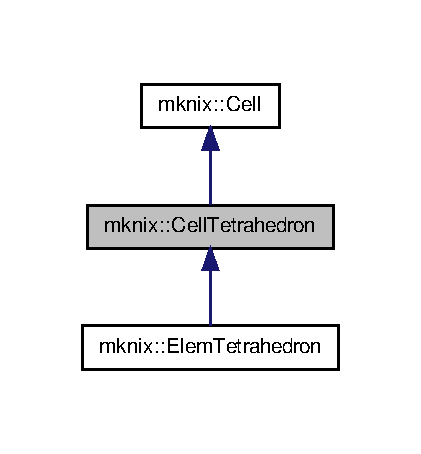
\includegraphics[width=203pt]{dd/d62/classmknix_1_1_cell_tetrahedron__inherit__graph}
\end{center}
\end{figure}


Collaboration diagram for mknix\+:\+:Cell\+Tetrahedron\+:\nopagebreak
\begin{figure}[H]
\begin{center}
\leavevmode
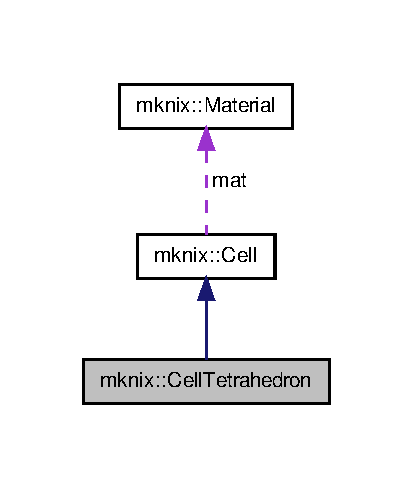
\includegraphics[width=198pt]{dc/db5/classmknix_1_1_cell_tetrahedron__coll__graph}
\end{center}
\end{figure}
\subsubsection*{Public Member Functions}
\begin{DoxyCompactItemize}
\item 
\hyperlink{classmknix_1_1_cell_tetrahedron_a6824b4f7304f0717ccdbaf32126239a0}{Cell\+Tetrahedron} ()
\item 
\hyperlink{classmknix_1_1_cell_tetrahedron_ac4c2343cfe88b0f0a0c2be8636fd0cde}{Cell\+Tetrahedron} (\hyperlink{classmknix_1_1_material}{Material} \&, std\+::string, double, int, \hyperlink{classmknix_1_1_point}{Point} $\ast$, \hyperlink{classmknix_1_1_point}{Point} $\ast$, \hyperlink{classmknix_1_1_point}{Point} $\ast$, \hyperlink{classmknix_1_1_point}{Point} $\ast$)
\item 
virtual \hyperlink{classmknix_1_1_cell_tetrahedron_a4ae5db633022a1714da463f4c32ffa03}{$\sim$\+Cell\+Tetrahedron} ()
\item 
void \hyperlink{classmknix_1_1_cell_tetrahedron_aba4f93f294a8ceea377cc2feb44f56db}{gnuplot\+Out} (std\+::ofstream \&, std\+::ofstream \&)
\end{DoxyCompactItemize}
\subsubsection*{Protected Member Functions}
\begin{DoxyCompactItemize}
\item 
void \hyperlink{classmknix_1_1_cell_tetrahedron_a933dde9cb028e9be1f0f9024fb7b898d}{create\+Gauss\+Points} ()
\end{DoxyCompactItemize}
\subsubsection*{Protected Attributes}
\begin{DoxyCompactItemize}
\item 
cofe\+::\+Tensor\+Rank2$<$ 3, double $>$ \hyperlink{classmknix_1_1_cell_tetrahedron_ad43ea7159ab2b6818636340c6f76de65}{points}
\end{DoxyCompactItemize}


\subsubsection{Detailed Description}
\begin{DoxyAuthor}{Author}
Daniel Iglesias 
\end{DoxyAuthor}


Definition at line 43 of file celltetrahedron.\+h.



\subsubsection{Constructor \& Destructor Documentation}
\hypertarget{classmknix_1_1_cell_tetrahedron_a6824b4f7304f0717ccdbaf32126239a0}{}\index{mknix\+::\+Cell\+Tetrahedron@{mknix\+::\+Cell\+Tetrahedron}!Cell\+Tetrahedron@{Cell\+Tetrahedron}}
\index{Cell\+Tetrahedron@{Cell\+Tetrahedron}!mknix\+::\+Cell\+Tetrahedron@{mknix\+::\+Cell\+Tetrahedron}}
\paragraph[{Cell\+Tetrahedron}]{\setlength{\rightskip}{0pt plus 5cm}mknix\+::\+Cell\+Tetrahedron\+::\+Cell\+Tetrahedron (
\begin{DoxyParamCaption}
{}
\end{DoxyParamCaption}
)}\label{classmknix_1_1_cell_tetrahedron_a6824b4f7304f0717ccdbaf32126239a0}


Definition at line 10 of file celltetrahedron.\+cpp.

\hypertarget{classmknix_1_1_cell_tetrahedron_ac4c2343cfe88b0f0a0c2be8636fd0cde}{}\index{mknix\+::\+Cell\+Tetrahedron@{mknix\+::\+Cell\+Tetrahedron}!Cell\+Tetrahedron@{Cell\+Tetrahedron}}
\index{Cell\+Tetrahedron@{Cell\+Tetrahedron}!mknix\+::\+Cell\+Tetrahedron@{mknix\+::\+Cell\+Tetrahedron}}
\paragraph[{Cell\+Tetrahedron}]{\setlength{\rightskip}{0pt plus 5cm}mknix\+::\+Cell\+Tetrahedron\+::\+Cell\+Tetrahedron (
\begin{DoxyParamCaption}
\item[{{\bf Material} \&}]{material\+\_\+in, }
\item[{std\+::string}]{formulation\+\_\+in, }
\item[{double}]{alpha\+\_\+in, }
\item[{int}]{n\+G\+Points\+\_\+in, }
\item[{{\bf Point} $\ast$}]{n1\+\_\+in, }
\item[{{\bf Point} $\ast$}]{n2\+\_\+in, }
\item[{{\bf Point} $\ast$}]{n3\+\_\+in, }
\item[{{\bf Point} $\ast$}]{n4\+\_\+in}
\end{DoxyParamCaption}
)}\label{classmknix_1_1_cell_tetrahedron_ac4c2343cfe88b0f0a0c2be8636fd0cde}


Definition at line 15 of file celltetrahedron.\+cpp.



Here is the call graph for this function\+:\nopagebreak
\begin{figure}[H]
\begin{center}
\leavevmode
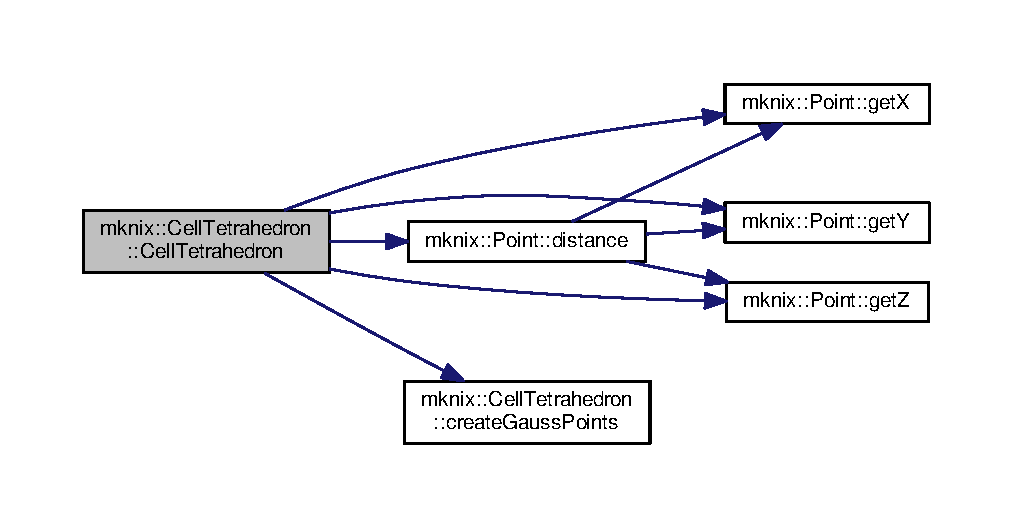
\includegraphics[width=350pt]{d9/d39/classmknix_1_1_cell_tetrahedron_ac4c2343cfe88b0f0a0c2be8636fd0cde_cgraph}
\end{center}
\end{figure}


\hypertarget{classmknix_1_1_cell_tetrahedron_a4ae5db633022a1714da463f4c32ffa03}{}\index{mknix\+::\+Cell\+Tetrahedron@{mknix\+::\+Cell\+Tetrahedron}!````~Cell\+Tetrahedron@{$\sim$\+Cell\+Tetrahedron}}
\index{````~Cell\+Tetrahedron@{$\sim$\+Cell\+Tetrahedron}!mknix\+::\+Cell\+Tetrahedron@{mknix\+::\+Cell\+Tetrahedron}}
\paragraph[{$\sim$\+Cell\+Tetrahedron}]{\setlength{\rightskip}{0pt plus 5cm}mknix\+::\+Cell\+Tetrahedron\+::$\sim$\+Cell\+Tetrahedron (
\begin{DoxyParamCaption}
{}
\end{DoxyParamCaption}
)\hspace{0.3cm}{\ttfamily [virtual]}}\label{classmknix_1_1_cell_tetrahedron_a4ae5db633022a1714da463f4c32ffa03}


Definition at line 65 of file celltetrahedron.\+cpp.



\subsubsection{Member Function Documentation}
\hypertarget{classmknix_1_1_cell_tetrahedron_a933dde9cb028e9be1f0f9024fb7b898d}{}\index{mknix\+::\+Cell\+Tetrahedron@{mknix\+::\+Cell\+Tetrahedron}!create\+Gauss\+Points@{create\+Gauss\+Points}}
\index{create\+Gauss\+Points@{create\+Gauss\+Points}!mknix\+::\+Cell\+Tetrahedron@{mknix\+::\+Cell\+Tetrahedron}}
\paragraph[{create\+Gauss\+Points}]{\setlength{\rightskip}{0pt plus 5cm}void mknix\+::\+Cell\+Tetrahedron\+::create\+Gauss\+Points (
\begin{DoxyParamCaption}
{}
\end{DoxyParamCaption}
)\hspace{0.3cm}{\ttfamily [protected]}}\label{classmknix_1_1_cell_tetrahedron_a933dde9cb028e9be1f0f9024fb7b898d}


Definition at line 70 of file celltetrahedron.\+cpp.



Here is the caller graph for this function\+:\nopagebreak
\begin{figure}[H]
\begin{center}
\leavevmode
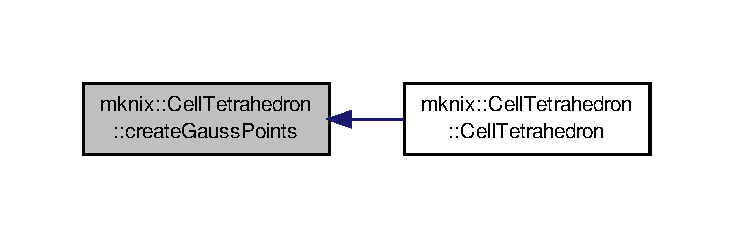
\includegraphics[width=350pt]{d9/d39/classmknix_1_1_cell_tetrahedron_a933dde9cb028e9be1f0f9024fb7b898d_icgraph}
\end{center}
\end{figure}


\hypertarget{classmknix_1_1_cell_tetrahedron_aba4f93f294a8ceea377cc2feb44f56db}{}\index{mknix\+::\+Cell\+Tetrahedron@{mknix\+::\+Cell\+Tetrahedron}!gnuplot\+Out@{gnuplot\+Out}}
\index{gnuplot\+Out@{gnuplot\+Out}!mknix\+::\+Cell\+Tetrahedron@{mknix\+::\+Cell\+Tetrahedron}}
\paragraph[{gnuplot\+Out}]{\setlength{\rightskip}{0pt plus 5cm}void mknix\+::\+Cell\+Tetrahedron\+::gnuplot\+Out (
\begin{DoxyParamCaption}
\item[{std\+::ofstream \&}]{data, }
\item[{std\+::ofstream \&}]{gpdata}
\end{DoxyParamCaption}
)\hspace{0.3cm}{\ttfamily [virtual]}}\label{classmknix_1_1_cell_tetrahedron_aba4f93f294a8ceea377cc2feb44f56db}


Implements \hyperlink{classmknix_1_1_cell_a345a938d058d10f60d6c302a715290de}{mknix\+::\+Cell}.



Definition at line 146 of file celltetrahedron.\+cpp.



\subsubsection{Member Data Documentation}
\hypertarget{classmknix_1_1_cell_tetrahedron_ad43ea7159ab2b6818636340c6f76de65}{}\index{mknix\+::\+Cell\+Tetrahedron@{mknix\+::\+Cell\+Tetrahedron}!points@{points}}
\index{points@{points}!mknix\+::\+Cell\+Tetrahedron@{mknix\+::\+Cell\+Tetrahedron}}
\paragraph[{points}]{\setlength{\rightskip}{0pt plus 5cm}cofe\+::\+Tensor\+Rank2$<$3, double$>$ mknix\+::\+Cell\+Tetrahedron\+::points\hspace{0.3cm}{\ttfamily [protected]}}\label{classmknix_1_1_cell_tetrahedron_ad43ea7159ab2b6818636340c6f76de65}
position of vertex points 

Definition at line 46 of file celltetrahedron.\+h.



The documentation for this class was generated from the following files\+:\begin{DoxyCompactItemize}
\item 
\hyperlink{celltetrahedron_8h}{celltetrahedron.\+h}\item 
\hyperlink{celltetrahedron_8cpp}{celltetrahedron.\+cpp}\end{DoxyCompactItemize}

\hypertarget{classmknix_1_1_cell_triang}{}\subsection{mknix\+:\+:Cell\+Triang Class Reference}
\label{classmknix_1_1_cell_triang}\index{mknix\+::\+Cell\+Triang@{mknix\+::\+Cell\+Triang}}


{\ttfamily \#include $<$celltriang.\+h$>$}



Inheritance diagram for mknix\+:\+:Cell\+Triang\+:\nopagebreak
\begin{figure}[H]
\begin{center}
\leavevmode
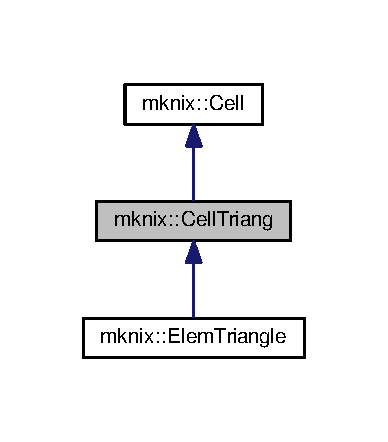
\includegraphics[width=186pt]{d9/d69/classmknix_1_1_cell_triang__inherit__graph}
\end{center}
\end{figure}


Collaboration diagram for mknix\+:\+:Cell\+Triang\+:\nopagebreak
\begin{figure}[H]
\begin{center}
\leavevmode
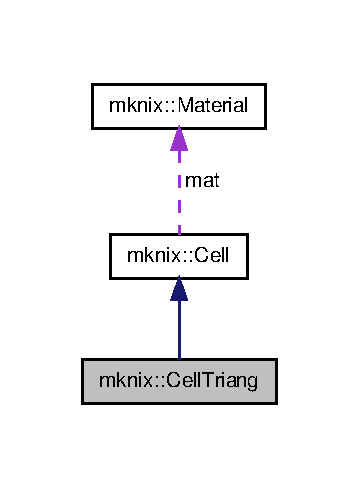
\includegraphics[width=173pt]{d0/db3/classmknix_1_1_cell_triang__coll__graph}
\end{center}
\end{figure}
\subsubsection*{Public Member Functions}
\begin{DoxyCompactItemize}
\item 
\hyperlink{classmknix_1_1_cell_triang_a17a2c3768e9f2aad3a7bfd8041775fb6}{Cell\+Triang} ()
\item 
\hyperlink{classmknix_1_1_cell_triang_a1d988a4f96b2f51d2a617fc105f9539b}{Cell\+Triang} (\hyperlink{classmknix_1_1_material}{Material} \&, std\+::string, double, int, \hyperlink{classmknix_1_1_point}{Point} $\ast$, \hyperlink{classmknix_1_1_point}{Point} $\ast$, \hyperlink{classmknix_1_1_point}{Point} $\ast$)
\item 
\hyperlink{classmknix_1_1_cell_triang_a745b852f45fac5becaeeca26b86123c9}{Cell\+Triang} (\hyperlink{classmknix_1_1_material}{Material} \&, std\+::string, double, int, \hyperlink{classmknix_1_1_point}{Point} $\ast$, \hyperlink{classmknix_1_1_point}{Point} $\ast$, \hyperlink{classmknix_1_1_point}{Point} $\ast$, double)
\item 
virtual \hyperlink{classmknix_1_1_cell_triang_af0a12b3f4f6106291f3252716c4be025}{$\sim$\+Cell\+Triang} ()
\item 
void \hyperlink{classmknix_1_1_cell_triang_a374f66822e2e37d94a2cfe09c5173e8a}{gnuplot\+Out} (std\+::ofstream \&, std\+::ofstream \&)
\end{DoxyCompactItemize}
\subsubsection*{Protected Member Functions}
\begin{DoxyCompactItemize}
\item 
void \hyperlink{classmknix_1_1_cell_triang_a2a2c65fbd2682eba8225473a7dc841f0}{create\+Gauss\+Points} ()
\end{DoxyCompactItemize}
\subsubsection*{Protected Attributes}
\begin{DoxyCompactItemize}
\item 
cofe\+::\+Tensor\+Rank2$<$ 3, double $>$ \hyperlink{classmknix_1_1_cell_triang_a22bff969ea4955bd817c94ae2915e60c}{points}
\end{DoxyCompactItemize}


\subsubsection{Detailed Description}
\begin{DoxyAuthor}{Author}
Daniel Iglesias 
\end{DoxyAuthor}


Definition at line 42 of file celltriang.\+h.



\subsubsection{Constructor \& Destructor Documentation}
\hypertarget{classmknix_1_1_cell_triang_a17a2c3768e9f2aad3a7bfd8041775fb6}{}\index{mknix\+::\+Cell\+Triang@{mknix\+::\+Cell\+Triang}!Cell\+Triang@{Cell\+Triang}}
\index{Cell\+Triang@{Cell\+Triang}!mknix\+::\+Cell\+Triang@{mknix\+::\+Cell\+Triang}}
\paragraph[{Cell\+Triang}]{\setlength{\rightskip}{0pt plus 5cm}mknix\+::\+Cell\+Triang\+::\+Cell\+Triang (
\begin{DoxyParamCaption}
{}
\end{DoxyParamCaption}
)}\label{classmknix_1_1_cell_triang_a17a2c3768e9f2aad3a7bfd8041775fb6}


Definition at line 9 of file celltriang.\+cpp.

\hypertarget{classmknix_1_1_cell_triang_a1d988a4f96b2f51d2a617fc105f9539b}{}\index{mknix\+::\+Cell\+Triang@{mknix\+::\+Cell\+Triang}!Cell\+Triang@{Cell\+Triang}}
\index{Cell\+Triang@{Cell\+Triang}!mknix\+::\+Cell\+Triang@{mknix\+::\+Cell\+Triang}}
\paragraph[{Cell\+Triang}]{\setlength{\rightskip}{0pt plus 5cm}mknix\+::\+Cell\+Triang\+::\+Cell\+Triang (
\begin{DoxyParamCaption}
\item[{{\bf Material} \&}]{material\+\_\+in, }
\item[{std\+::string}]{formulation\+\_\+in, }
\item[{double}]{alpha\+\_\+in, }
\item[{int}]{n\+G\+Points\+\_\+in, }
\item[{{\bf Point} $\ast$}]{n1\+\_\+in, }
\item[{{\bf Point} $\ast$}]{n2\+\_\+in, }
\item[{{\bf Point} $\ast$}]{n3\+\_\+in}
\end{DoxyParamCaption}
)}\label{classmknix_1_1_cell_triang_a1d988a4f96b2f51d2a617fc105f9539b}


Definition at line 14 of file celltriang.\+cpp.



Here is the call graph for this function\+:\nopagebreak
\begin{figure}[H]
\begin{center}
\leavevmode
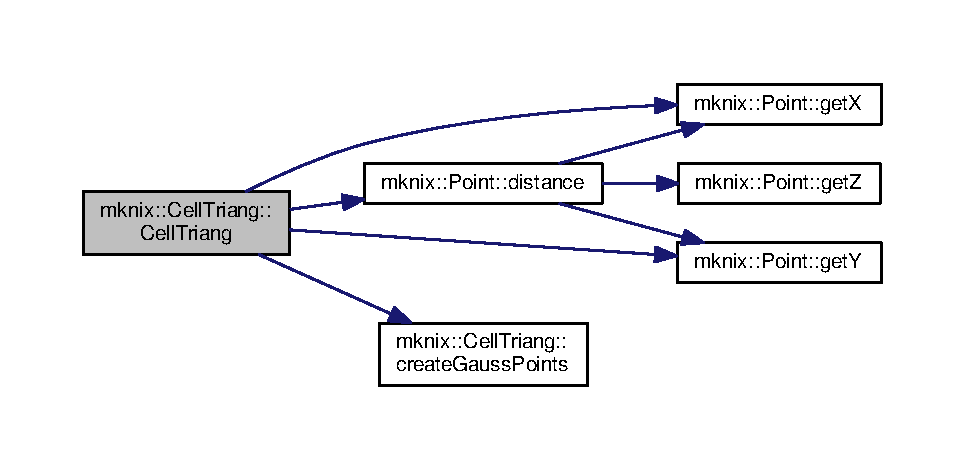
\includegraphics[width=350pt]{de/db4/classmknix_1_1_cell_triang_a1d988a4f96b2f51d2a617fc105f9539b_cgraph}
\end{center}
\end{figure}


\hypertarget{classmknix_1_1_cell_triang_a745b852f45fac5becaeeca26b86123c9}{}\index{mknix\+::\+Cell\+Triang@{mknix\+::\+Cell\+Triang}!Cell\+Triang@{Cell\+Triang}}
\index{Cell\+Triang@{Cell\+Triang}!mknix\+::\+Cell\+Triang@{mknix\+::\+Cell\+Triang}}
\paragraph[{Cell\+Triang}]{\setlength{\rightskip}{0pt plus 5cm}mknix\+::\+Cell\+Triang\+::\+Cell\+Triang (
\begin{DoxyParamCaption}
\item[{{\bf Material} \&}]{material\+\_\+in, }
\item[{std\+::string}]{formulation\+\_\+in, }
\item[{double}]{alpha\+\_\+in, }
\item[{int}]{n\+G\+Points\+\_\+in, }
\item[{{\bf Point} $\ast$}]{n1\+\_\+in, }
\item[{{\bf Point} $\ast$}]{n2\+\_\+in, }
\item[{{\bf Point} $\ast$}]{n3\+\_\+in, }
\item[{double}]{dc\+\_\+in}
\end{DoxyParamCaption}
)}\label{classmknix_1_1_cell_triang_a745b852f45fac5becaeeca26b86123c9}


Definition at line 48 of file celltriang.\+cpp.



Here is the call graph for this function\+:\nopagebreak
\begin{figure}[H]
\begin{center}
\leavevmode
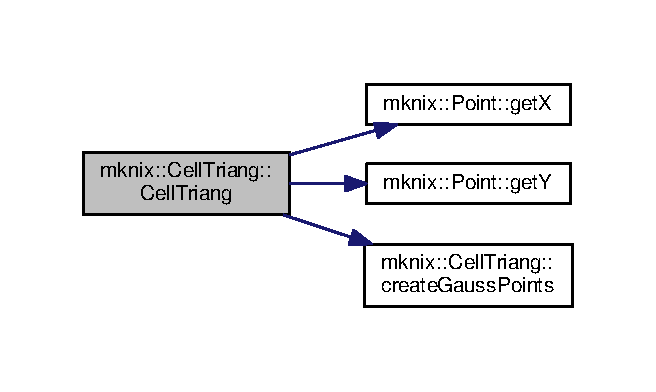
\includegraphics[width=315pt]{de/db4/classmknix_1_1_cell_triang_a745b852f45fac5becaeeca26b86123c9_cgraph}
\end{center}
\end{figure}


\hypertarget{classmknix_1_1_cell_triang_af0a12b3f4f6106291f3252716c4be025}{}\index{mknix\+::\+Cell\+Triang@{mknix\+::\+Cell\+Triang}!````~Cell\+Triang@{$\sim$\+Cell\+Triang}}
\index{````~Cell\+Triang@{$\sim$\+Cell\+Triang}!mknix\+::\+Cell\+Triang@{mknix\+::\+Cell\+Triang}}
\paragraph[{$\sim$\+Cell\+Triang}]{\setlength{\rightskip}{0pt plus 5cm}mknix\+::\+Cell\+Triang\+::$\sim$\+Cell\+Triang (
\begin{DoxyParamCaption}
{}
\end{DoxyParamCaption}
)\hspace{0.3cm}{\ttfamily [virtual]}}\label{classmknix_1_1_cell_triang_af0a12b3f4f6106291f3252716c4be025}


Definition at line 81 of file celltriang.\+cpp.



\subsubsection{Member Function Documentation}
\hypertarget{classmknix_1_1_cell_triang_a2a2c65fbd2682eba8225473a7dc841f0}{}\index{mknix\+::\+Cell\+Triang@{mknix\+::\+Cell\+Triang}!create\+Gauss\+Points@{create\+Gauss\+Points}}
\index{create\+Gauss\+Points@{create\+Gauss\+Points}!mknix\+::\+Cell\+Triang@{mknix\+::\+Cell\+Triang}}
\paragraph[{create\+Gauss\+Points}]{\setlength{\rightskip}{0pt plus 5cm}void mknix\+::\+Cell\+Triang\+::create\+Gauss\+Points (
\begin{DoxyParamCaption}
{}
\end{DoxyParamCaption}
)\hspace{0.3cm}{\ttfamily [protected]}}\label{classmknix_1_1_cell_triang_a2a2c65fbd2682eba8225473a7dc841f0}


Definition at line 86 of file celltriang.\+cpp.



Here is the caller graph for this function\+:\nopagebreak
\begin{figure}[H]
\begin{center}
\leavevmode
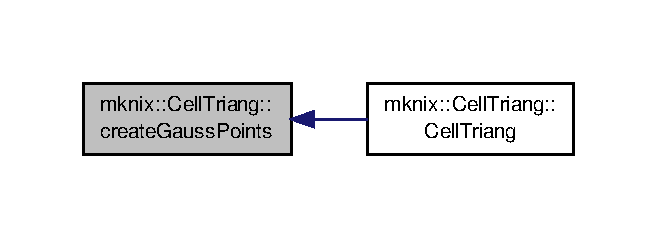
\includegraphics[width=315pt]{de/db4/classmknix_1_1_cell_triang_a2a2c65fbd2682eba8225473a7dc841f0_icgraph}
\end{center}
\end{figure}


\hypertarget{classmknix_1_1_cell_triang_a374f66822e2e37d94a2cfe09c5173e8a}{}\index{mknix\+::\+Cell\+Triang@{mknix\+::\+Cell\+Triang}!gnuplot\+Out@{gnuplot\+Out}}
\index{gnuplot\+Out@{gnuplot\+Out}!mknix\+::\+Cell\+Triang@{mknix\+::\+Cell\+Triang}}
\paragraph[{gnuplot\+Out}]{\setlength{\rightskip}{0pt plus 5cm}void mknix\+::\+Cell\+Triang\+::gnuplot\+Out (
\begin{DoxyParamCaption}
\item[{std\+::ofstream \&}]{data, }
\item[{std\+::ofstream \&}]{gpdata}
\end{DoxyParamCaption}
)\hspace{0.3cm}{\ttfamily [virtual]}}\label{classmknix_1_1_cell_triang_a374f66822e2e37d94a2cfe09c5173e8a}


Implements \hyperlink{classmknix_1_1_cell_a345a938d058d10f60d6c302a715290de}{mknix\+::\+Cell}.



Definition at line 288 of file celltriang.\+cpp.



\subsubsection{Member Data Documentation}
\hypertarget{classmknix_1_1_cell_triang_a22bff969ea4955bd817c94ae2915e60c}{}\index{mknix\+::\+Cell\+Triang@{mknix\+::\+Cell\+Triang}!points@{points}}
\index{points@{points}!mknix\+::\+Cell\+Triang@{mknix\+::\+Cell\+Triang}}
\paragraph[{points}]{\setlength{\rightskip}{0pt plus 5cm}cofe\+::\+Tensor\+Rank2$<$3, double$>$ mknix\+::\+Cell\+Triang\+::points\hspace{0.3cm}{\ttfamily [protected]}}\label{classmknix_1_1_cell_triang_a22bff969ea4955bd817c94ae2915e60c}
position of vertex points 

Definition at line 45 of file celltriang.\+h.



The documentation for this class was generated from the following files\+:\begin{DoxyCompactItemize}
\item 
\hyperlink{celltriang_8h}{celltriang.\+h}\item 
\hyperlink{celltriang_8cpp}{celltriang.\+cpp}\end{DoxyCompactItemize}

\hypertarget{classmknix_1_1_comp_bar}{\subsection{mknix\-:\-:Comp\-Bar Class Reference}
\label{classmknix_1_1_comp_bar}\index{mknix\-::\-Comp\-Bar@{mknix\-::\-Comp\-Bar}}
}


{\ttfamily \#include $<$compbar.\-h$>$}

\subsubsection*{Public Member Functions}
\begin{DoxyCompactItemize}
\item 
\hyperlink{classmknix_1_1_comp_bar_ab72db97465fe7f1bfa97204bad5528c3}{Comp\-Bar} ()
\item 
\hyperlink{classmknix_1_1_comp_bar_afdb8c9aeaa0ac6aec90075dad6e35c92}{Comp\-Bar} (int, \hyperlink{classmknix_1_1_node}{Node} $\ast$, \hyperlink{classmknix_1_1_node}{Node} $\ast$)
\item 
\hyperlink{classmknix_1_1_comp_bar_aad258dca0df1e017f189fc743baaf150}{$\sim$\-Comp\-Bar} ()
\item 
void \hyperlink{classmknix_1_1_comp_bar_adb7f828038ec2b850d93af242ce29faa}{add\-To\-Render} (vtk\-Renderer $\ast$)
\item 
void \hyperlink{classmknix_1_1_comp_bar_a8642880b1f8a552dc2e955dcf9f31331}{remove\-From\-Render} (vtk\-Renderer $\ast$)
\item 
void \hyperlink{classmknix_1_1_comp_bar_aadfecc285b6aecc94d45df348f1974b3}{actualize\-Points} ()
\end{DoxyCompactItemize}


\subsubsection{Constructor \& Destructor Documentation}
\hypertarget{classmknix_1_1_comp_bar_ab72db97465fe7f1bfa97204bad5528c3}{\index{mknix\-::\-Comp\-Bar@{mknix\-::\-Comp\-Bar}!Comp\-Bar@{Comp\-Bar}}
\index{Comp\-Bar@{Comp\-Bar}!mknix::CompBar@{mknix\-::\-Comp\-Bar}}
\paragraph[{Comp\-Bar}]{\setlength{\rightskip}{0pt plus 5cm}mknix\-::\-Comp\-Bar\-::\-Comp\-Bar (
\begin{DoxyParamCaption}
{}
\end{DoxyParamCaption}
)}}\label{classmknix_1_1_comp_bar_ab72db97465fe7f1bfa97204bad5528c3}
\hypertarget{classmknix_1_1_comp_bar_afdb8c9aeaa0ac6aec90075dad6e35c92}{\index{mknix\-::\-Comp\-Bar@{mknix\-::\-Comp\-Bar}!Comp\-Bar@{Comp\-Bar}}
\index{Comp\-Bar@{Comp\-Bar}!mknix::CompBar@{mknix\-::\-Comp\-Bar}}
\paragraph[{Comp\-Bar}]{\setlength{\rightskip}{0pt plus 5cm}mknix\-::\-Comp\-Bar\-::\-Comp\-Bar (
\begin{DoxyParamCaption}
\item[{int}]{mat\-\_\-in, }
\item[{{\bf Node} $\ast$}]{node\-A\-\_\-in, }
\item[{{\bf Node} $\ast$}]{node\-B\-\_\-in}
\end{DoxyParamCaption}
)}}\label{classmknix_1_1_comp_bar_afdb8c9aeaa0ac6aec90075dad6e35c92}


Here is the call graph for this function\-:\nopagebreak
\begin{figure}[H]
\begin{center}
\leavevmode
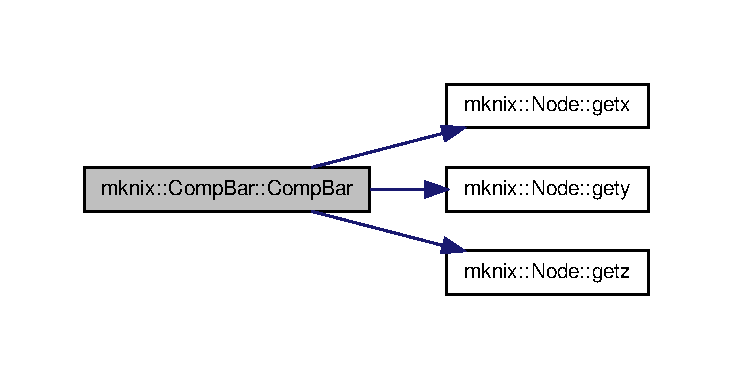
\includegraphics[width=350pt]{d1/d90/classmknix_1_1_comp_bar_afdb8c9aeaa0ac6aec90075dad6e35c92_cgraph}
\end{center}
\end{figure}


\hypertarget{classmknix_1_1_comp_bar_aad258dca0df1e017f189fc743baaf150}{\index{mknix\-::\-Comp\-Bar@{mknix\-::\-Comp\-Bar}!$\sim$\-Comp\-Bar@{$\sim$\-Comp\-Bar}}
\index{$\sim$\-Comp\-Bar@{$\sim$\-Comp\-Bar}!mknix::CompBar@{mknix\-::\-Comp\-Bar}}
\paragraph[{$\sim$\-Comp\-Bar}]{\setlength{\rightskip}{0pt plus 5cm}mknix\-::\-Comp\-Bar\-::$\sim$\-Comp\-Bar (
\begin{DoxyParamCaption}
{}
\end{DoxyParamCaption}
)}}\label{classmknix_1_1_comp_bar_aad258dca0df1e017f189fc743baaf150}


\subsubsection{Member Function Documentation}
\hypertarget{classmknix_1_1_comp_bar_aadfecc285b6aecc94d45df348f1974b3}{\index{mknix\-::\-Comp\-Bar@{mknix\-::\-Comp\-Bar}!actualize\-Points@{actualize\-Points}}
\index{actualize\-Points@{actualize\-Points}!mknix::CompBar@{mknix\-::\-Comp\-Bar}}
\paragraph[{actualize\-Points}]{\setlength{\rightskip}{0pt plus 5cm}void mknix\-::\-Comp\-Bar\-::actualize\-Points (
\begin{DoxyParamCaption}
{}
\end{DoxyParamCaption}
)}}\label{classmknix_1_1_comp_bar_aadfecc285b6aecc94d45df348f1974b3}


Here is the call graph for this function\-:\nopagebreak
\begin{figure}[H]
\begin{center}
\leavevmode
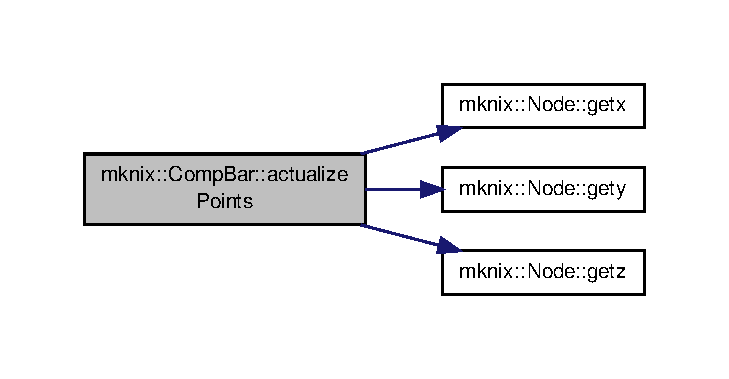
\includegraphics[width=350pt]{d1/d90/classmknix_1_1_comp_bar_aadfecc285b6aecc94d45df348f1974b3_cgraph}
\end{center}
\end{figure}


\hypertarget{classmknix_1_1_comp_bar_adb7f828038ec2b850d93af242ce29faa}{\index{mknix\-::\-Comp\-Bar@{mknix\-::\-Comp\-Bar}!add\-To\-Render@{add\-To\-Render}}
\index{add\-To\-Render@{add\-To\-Render}!mknix::CompBar@{mknix\-::\-Comp\-Bar}}
\paragraph[{add\-To\-Render}]{\setlength{\rightskip}{0pt plus 5cm}void mknix\-::\-Comp\-Bar\-::add\-To\-Render (
\begin{DoxyParamCaption}
\item[{vtk\-Renderer $\ast$}]{renderer\-\_\-in}
\end{DoxyParamCaption}
)}}\label{classmknix_1_1_comp_bar_adb7f828038ec2b850d93af242ce29faa}
\hypertarget{classmknix_1_1_comp_bar_a8642880b1f8a552dc2e955dcf9f31331}{\index{mknix\-::\-Comp\-Bar@{mknix\-::\-Comp\-Bar}!remove\-From\-Render@{remove\-From\-Render}}
\index{remove\-From\-Render@{remove\-From\-Render}!mknix::CompBar@{mknix\-::\-Comp\-Bar}}
\paragraph[{remove\-From\-Render}]{\setlength{\rightskip}{0pt plus 5cm}void mknix\-::\-Comp\-Bar\-::remove\-From\-Render (
\begin{DoxyParamCaption}
\item[{vtk\-Renderer $\ast$}]{renderer\-\_\-in}
\end{DoxyParamCaption}
)}}\label{classmknix_1_1_comp_bar_a8642880b1f8a552dc2e955dcf9f31331}


The documentation for this class was generated from the following files\-:\begin{DoxyCompactItemize}
\item 
\hyperlink{compbar_8h}{compbar.\-h}\item 
\hyperlink{compbar_8cpp}{compbar.\-cpp}\end{DoxyCompactItemize}

\hypertarget{classmknix_1_1_constraint}{\subsection{mknix\-:\-:Constraint Class Reference}
\label{classmknix_1_1_constraint}\index{mknix\-::\-Constraint@{mknix\-::\-Constraint}}
}


{\ttfamily \#include $<$constraint.\-h$>$}



Inheritance diagram for mknix\-:\-:Constraint\-:\nopagebreak
\begin{figure}[H]
\begin{center}
\leavevmode
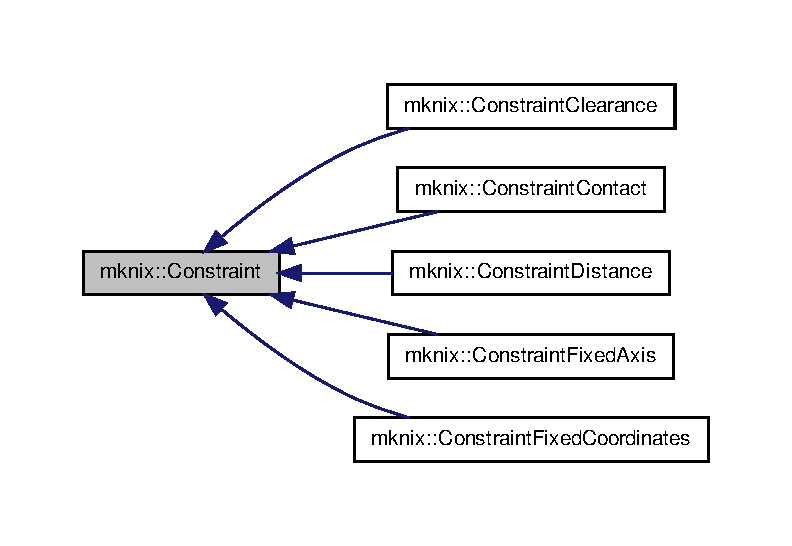
\includegraphics[width=350pt]{db/d85/classmknix_1_1_constraint__inherit__graph}
\end{center}
\end{figure}
\subsubsection*{Public Member Functions}
\begin{DoxyCompactItemize}
\item 
\hyperlink{classmknix_1_1_constraint_ae4a69ed64d7746a7f8e2d23f04bc6de6}{Constraint} ()
\item 
\hyperlink{classmknix_1_1_constraint_a093b4ffce363485f60ba251356ff88d1}{Constraint} (double \&, std\-::string \&)
\item 
virtual \hyperlink{classmknix_1_1_constraint_a84cbe5af8074dc229f583d119bbde3e1}{$\sim$\-Constraint} ()
\item 
virtual void \hyperlink{classmknix_1_1_constraint_a7f2b34d256d5eec54b34b0440b562ec1}{calc\-Phi} ()=0
\item 
virtual void \hyperlink{classmknix_1_1_constraint_ab129143960df2b9459e274275608bcf2}{calc\-Phiq} ()=0
\item 
virtual void \hyperlink{classmknix_1_1_constraint_a73ff21573b5e9c4acda789bd5ac46ea8}{calc\-Phiqq} ()=0
\item 
virtual void \hyperlink{classmknix_1_1_constraint_a00ea21a19168bc3cfd3ba97c6a2be31d}{calc\-Internal\-Forces} ()
\item 
virtual void \hyperlink{classmknix_1_1_constraint_a9b7594c65aa792ffb56d3a598996a969}{calc\-Tangent\-Matrix} ()
\item 
virtual void \hyperlink{classmknix_1_1_constraint_aca5d35f6ecd8f8f3852c150c7901b890}{assemble\-Internal\-Forces} (lmx\-::\-Vector$<$ \hyperlink{namespacemknix_a16be4b246fbf2cceb141e3a179111020}{data\-\_\-type} $>$ \&)
\item 
virtual void \hyperlink{classmknix_1_1_constraint_ac376643d6d73cb3b591ba80aae9f7166}{assemble\-Tangent\-Matrix} (lmx\-::\-Matrix$<$ \hyperlink{namespacemknix_a16be4b246fbf2cceb141e3a179111020}{data\-\_\-type} $>$ \&)
\item 
virtual bool \hyperlink{classmknix_1_1_constraint_a26923b449734b9f11ed5ca2556585dcb}{check\-Augmented} ()
\item 
virtual void \hyperlink{classmknix_1_1_constraint_a2e1f0de7e983151fb892468774dcdf12}{clear\-Augmented} ()
\item 
virtual \hyperlink{classmknix_1_1_node}{Node} $\ast$ \hyperlink{classmknix_1_1_constraint_a0e81d924dad26b7b5b0749d4580dd63c}{get\-Node} (int node\-Number)
\end{DoxyCompactItemize}
\subsubsection*{Protected Attributes}
\begin{DoxyCompactItemize}
\item 
int \hyperlink{classmknix_1_1_constraint_a5fa3727603b390206e6431141b892517}{dim}
\item 
double \hyperlink{classmknix_1_1_constraint_ab76845f20e7a29693b9161e09074d55a}{alpha}
\item 
std\-::string \hyperlink{classmknix_1_1_constraint_ab05c0dcc5cc535f4e3bed2fd34ed6d75}{method}
\item 
std\-::vector$<$ \hyperlink{classmknix_1_1_node}{Node} $\ast$ $>$ \hyperlink{classmknix_1_1_constraint_aa4aa16e121963acf4c086f63137d4ac1}{nodes}
\item 
lmx\-::\-Vector$<$ \hyperlink{namespacemknix_a16be4b246fbf2cceb141e3a179111020}{data\-\_\-type} $>$ \hyperlink{classmknix_1_1_constraint_a0b0fbbf149c32ce0a9dd6e0c4dd5851e}{internal\-Forces}
\item 
lmx\-::\-Dense\-Matrix$<$ \hyperlink{namespacemknix_a16be4b246fbf2cceb141e3a179111020}{data\-\_\-type} $>$ \hyperlink{classmknix_1_1_constraint_ab4b508cdbea36124b925f52525a1d5ad}{stiffness\-Matrix}
\item 
std\-::vector$<$ double $>$ \hyperlink{classmknix_1_1_constraint_aeee7c3bdd61194e3df0e958ff237040a}{lambda}
\item 
std\-::vector$<$ double $>$ \hyperlink{classmknix_1_1_constraint_a10e027fc12cb248a49a1ded049f0a161}{phi}
\item 
std\-::vector$<$ lmx\-::\-Vector\\*
$<$ \hyperlink{namespacemknix_a16be4b246fbf2cceb141e3a179111020}{data\-\_\-type} $>$ $>$ \hyperlink{classmknix_1_1_constraint_a667ecb78177b06981c30e23cb194b806}{phi\-\_\-q}
\item 
std\-::vector$<$ lmx\-::\-Dense\-Matrix\\*
$<$ \hyperlink{namespacemknix_a16be4b246fbf2cceb141e3a179111020}{data\-\_\-type} $>$ $>$ \hyperlink{classmknix_1_1_constraint_a9173b52da189652951ce51b1d69fcde4}{phi\-\_\-qq}
\end{DoxyCompactItemize}


\subsubsection{Detailed Description}
\begin{DoxyAuthor}{Author}
A\-U\-T\-H\-O\-R\-S $<$\-M\-A\-I\-L\-S$>$ 
\end{DoxyAuthor}


\subsubsection{Constructor \& Destructor Documentation}
\hypertarget{classmknix_1_1_constraint_ae4a69ed64d7746a7f8e2d23f04bc6de6}{\index{mknix\-::\-Constraint@{mknix\-::\-Constraint}!Constraint@{Constraint}}
\index{Constraint@{Constraint}!mknix::Constraint@{mknix\-::\-Constraint}}
\paragraph[{Constraint}]{\setlength{\rightskip}{0pt plus 5cm}mknix\-::\-Constraint\-::\-Constraint (
\begin{DoxyParamCaption}
{}
\end{DoxyParamCaption}
)}}\label{classmknix_1_1_constraint_ae4a69ed64d7746a7f8e2d23f04bc6de6}
\hypertarget{classmknix_1_1_constraint_a093b4ffce363485f60ba251356ff88d1}{\index{mknix\-::\-Constraint@{mknix\-::\-Constraint}!Constraint@{Constraint}}
\index{Constraint@{Constraint}!mknix::Constraint@{mknix\-::\-Constraint}}
\paragraph[{Constraint}]{\setlength{\rightskip}{0pt plus 5cm}mknix\-::\-Constraint\-::\-Constraint (
\begin{DoxyParamCaption}
\item[{double \&}]{alpha\-\_\-in, }
\item[{std\-::string \&}]{method\-\_\-in}
\end{DoxyParamCaption}
)}}\label{classmknix_1_1_constraint_a093b4ffce363485f60ba251356ff88d1}
\hypertarget{classmknix_1_1_constraint_a84cbe5af8074dc229f583d119bbde3e1}{\index{mknix\-::\-Constraint@{mknix\-::\-Constraint}!$\sim$\-Constraint@{$\sim$\-Constraint}}
\index{$\sim$\-Constraint@{$\sim$\-Constraint}!mknix::Constraint@{mknix\-::\-Constraint}}
\paragraph[{$\sim$\-Constraint}]{\setlength{\rightskip}{0pt plus 5cm}mknix\-::\-Constraint\-::$\sim$\-Constraint (
\begin{DoxyParamCaption}
{}
\end{DoxyParamCaption}
)\hspace{0.3cm}{\ttfamily [virtual]}}}\label{classmknix_1_1_constraint_a84cbe5af8074dc229f583d119bbde3e1}


\subsubsection{Member Function Documentation}
\hypertarget{classmknix_1_1_constraint_aca5d35f6ecd8f8f3852c150c7901b890}{\index{mknix\-::\-Constraint@{mknix\-::\-Constraint}!assemble\-Internal\-Forces@{assemble\-Internal\-Forces}}
\index{assemble\-Internal\-Forces@{assemble\-Internal\-Forces}!mknix::Constraint@{mknix\-::\-Constraint}}
\paragraph[{assemble\-Internal\-Forces}]{\setlength{\rightskip}{0pt plus 5cm}void mknix\-::\-Constraint\-::assemble\-Internal\-Forces (
\begin{DoxyParamCaption}
\item[{lmx\-::\-Vector$<$ {\bf data\-\_\-type} $>$ \&}]{global\-Internal\-Forces}
\end{DoxyParamCaption}
)\hspace{0.3cm}{\ttfamily [virtual]}}}\label{classmknix_1_1_constraint_aca5d35f6ecd8f8f3852c150c7901b890}


Here is the call graph for this function\-:\nopagebreak
\begin{figure}[H]
\begin{center}
\leavevmode
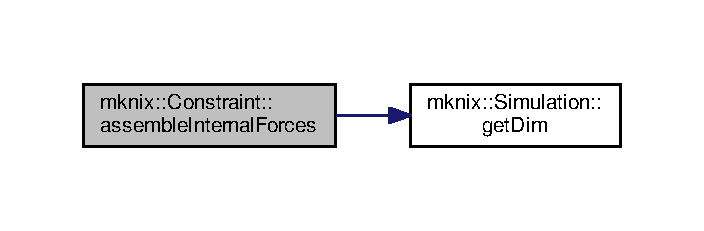
\includegraphics[width=340pt]{da/dd3/classmknix_1_1_constraint_aca5d35f6ecd8f8f3852c150c7901b890_cgraph}
\end{center}
\end{figure}


\hypertarget{classmknix_1_1_constraint_ac376643d6d73cb3b591ba80aae9f7166}{\index{mknix\-::\-Constraint@{mknix\-::\-Constraint}!assemble\-Tangent\-Matrix@{assemble\-Tangent\-Matrix}}
\index{assemble\-Tangent\-Matrix@{assemble\-Tangent\-Matrix}!mknix::Constraint@{mknix\-::\-Constraint}}
\paragraph[{assemble\-Tangent\-Matrix}]{\setlength{\rightskip}{0pt plus 5cm}void mknix\-::\-Constraint\-::assemble\-Tangent\-Matrix (
\begin{DoxyParamCaption}
\item[{lmx\-::\-Matrix$<$ {\bf data\-\_\-type} $>$ \&}]{global\-Tangent}
\end{DoxyParamCaption}
)\hspace{0.3cm}{\ttfamily [virtual]}}}\label{classmknix_1_1_constraint_ac376643d6d73cb3b591ba80aae9f7166}


Here is the call graph for this function\-:\nopagebreak
\begin{figure}[H]
\begin{center}
\leavevmode
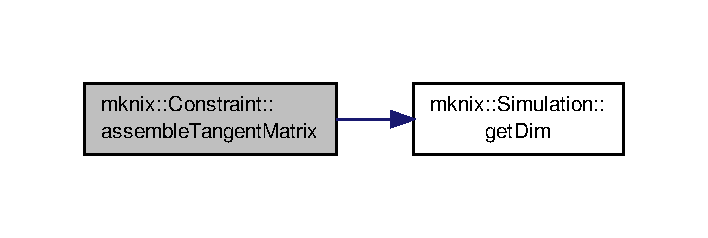
\includegraphics[width=340pt]{da/dd3/classmknix_1_1_constraint_ac376643d6d73cb3b591ba80aae9f7166_cgraph}
\end{center}
\end{figure}


\hypertarget{classmknix_1_1_constraint_a00ea21a19168bc3cfd3ba97c6a2be31d}{\index{mknix\-::\-Constraint@{mknix\-::\-Constraint}!calc\-Internal\-Forces@{calc\-Internal\-Forces}}
\index{calc\-Internal\-Forces@{calc\-Internal\-Forces}!mknix::Constraint@{mknix\-::\-Constraint}}
\paragraph[{calc\-Internal\-Forces}]{\setlength{\rightskip}{0pt plus 5cm}void mknix\-::\-Constraint\-::calc\-Internal\-Forces (
\begin{DoxyParamCaption}
{}
\end{DoxyParamCaption}
)\hspace{0.3cm}{\ttfamily [virtual]}}}\label{classmknix_1_1_constraint_a00ea21a19168bc3cfd3ba97c6a2be31d}


Here is the call graph for this function\-:\nopagebreak
\begin{figure}[H]
\begin{center}
\leavevmode
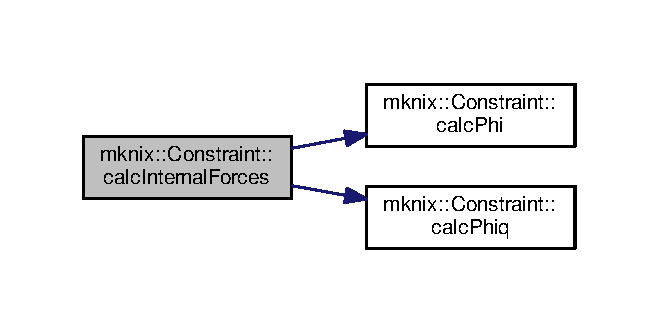
\includegraphics[width=316pt]{da/dd3/classmknix_1_1_constraint_a00ea21a19168bc3cfd3ba97c6a2be31d_cgraph}
\end{center}
\end{figure}


\hypertarget{classmknix_1_1_constraint_a7f2b34d256d5eec54b34b0440b562ec1}{\index{mknix\-::\-Constraint@{mknix\-::\-Constraint}!calc\-Phi@{calc\-Phi}}
\index{calc\-Phi@{calc\-Phi}!mknix::Constraint@{mknix\-::\-Constraint}}
\paragraph[{calc\-Phi}]{\setlength{\rightskip}{0pt plus 5cm}virtual void mknix\-::\-Constraint\-::calc\-Phi (
\begin{DoxyParamCaption}
{}
\end{DoxyParamCaption}
)\hspace{0.3cm}{\ttfamily [pure virtual]}}}\label{classmknix_1_1_constraint_a7f2b34d256d5eec54b34b0440b562ec1}


Implemented in \hyperlink{classmknix_1_1_constraint_distance_ad838af34d5ada5ba2f4ce559a472e16a}{mknix\-::\-Constraint\-Distance}, \hyperlink{classmknix_1_1_constraint_clearance_adeab95be15eee6fe28f09fafd4f5757a}{mknix\-::\-Constraint\-Clearance}, \hyperlink{classmknix_1_1_constraint_contact_a21a89037754ef5d968bda199ad3f1858}{mknix\-::\-Constraint\-Contact}, \hyperlink{classmknix_1_1_constraint_fixed_axis_ab5f59fd55877e45184aa90787479415c}{mknix\-::\-Constraint\-Fixed\-Axis}, and \hyperlink{classmknix_1_1_constraint_fixed_coordinates_ae549d41c12fcc094bdc32bc853ebbd84}{mknix\-::\-Constraint\-Fixed\-Coordinates}.



Here is the caller graph for this function\-:\nopagebreak
\begin{figure}[H]
\begin{center}
\leavevmode
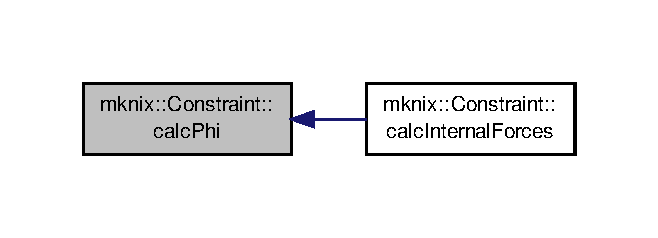
\includegraphics[width=316pt]{da/dd3/classmknix_1_1_constraint_a7f2b34d256d5eec54b34b0440b562ec1_icgraph}
\end{center}
\end{figure}


\hypertarget{classmknix_1_1_constraint_ab129143960df2b9459e274275608bcf2}{\index{mknix\-::\-Constraint@{mknix\-::\-Constraint}!calc\-Phiq@{calc\-Phiq}}
\index{calc\-Phiq@{calc\-Phiq}!mknix::Constraint@{mknix\-::\-Constraint}}
\paragraph[{calc\-Phiq}]{\setlength{\rightskip}{0pt plus 5cm}virtual void mknix\-::\-Constraint\-::calc\-Phiq (
\begin{DoxyParamCaption}
{}
\end{DoxyParamCaption}
)\hspace{0.3cm}{\ttfamily [pure virtual]}}}\label{classmknix_1_1_constraint_ab129143960df2b9459e274275608bcf2}


Implemented in \hyperlink{classmknix_1_1_constraint_distance_a6fa6c37266c01a1e8f577418dd886037}{mknix\-::\-Constraint\-Distance}, \hyperlink{classmknix_1_1_constraint_clearance_a7e834e62ef642f4f5207f3021f11020e}{mknix\-::\-Constraint\-Clearance}, \hyperlink{classmknix_1_1_constraint_contact_a88c495ea01a5f8f8807dd72ae3e7240f}{mknix\-::\-Constraint\-Contact}, \hyperlink{classmknix_1_1_constraint_fixed_axis_a40970d2c0103244ac5e75307247d25b9}{mknix\-::\-Constraint\-Fixed\-Axis}, and \hyperlink{classmknix_1_1_constraint_fixed_coordinates_a250813aed17ab80b03a9b6b7f4a7ce8b}{mknix\-::\-Constraint\-Fixed\-Coordinates}.



Here is the caller graph for this function\-:\nopagebreak
\begin{figure}[H]
\begin{center}
\leavevmode
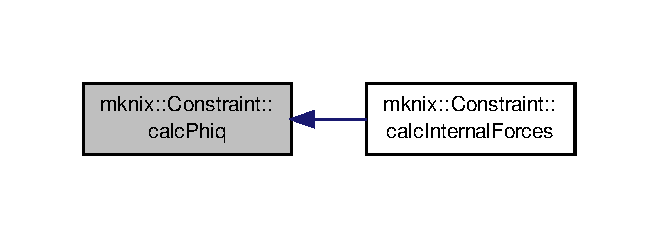
\includegraphics[width=316pt]{da/dd3/classmknix_1_1_constraint_ab129143960df2b9459e274275608bcf2_icgraph}
\end{center}
\end{figure}


\hypertarget{classmknix_1_1_constraint_a73ff21573b5e9c4acda789bd5ac46ea8}{\index{mknix\-::\-Constraint@{mknix\-::\-Constraint}!calc\-Phiqq@{calc\-Phiqq}}
\index{calc\-Phiqq@{calc\-Phiqq}!mknix::Constraint@{mknix\-::\-Constraint}}
\paragraph[{calc\-Phiqq}]{\setlength{\rightskip}{0pt plus 5cm}virtual void mknix\-::\-Constraint\-::calc\-Phiqq (
\begin{DoxyParamCaption}
{}
\end{DoxyParamCaption}
)\hspace{0.3cm}{\ttfamily [pure virtual]}}}\label{classmknix_1_1_constraint_a73ff21573b5e9c4acda789bd5ac46ea8}


Implemented in \hyperlink{classmknix_1_1_constraint_distance_ad4d1eb206239508f7f2f5b4d26b957eb}{mknix\-::\-Constraint\-Distance}, \hyperlink{classmknix_1_1_constraint_clearance_aea75fa1da7455bbefb5ce7705a16a3cc}{mknix\-::\-Constraint\-Clearance}, \hyperlink{classmknix_1_1_constraint_contact_ad9b4db34bf76f2d8ea9532d5d3e0449f}{mknix\-::\-Constraint\-Contact}, \hyperlink{classmknix_1_1_constraint_fixed_axis_a10444d42c4401cf093b221d59354ab8b}{mknix\-::\-Constraint\-Fixed\-Axis}, and \hyperlink{classmknix_1_1_constraint_fixed_coordinates_a80e20da8642dc3c35b7969f7c2c5affe}{mknix\-::\-Constraint\-Fixed\-Coordinates}.



Here is the caller graph for this function\-:\nopagebreak
\begin{figure}[H]
\begin{center}
\leavevmode
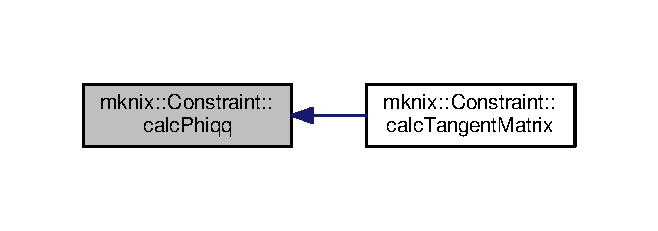
\includegraphics[width=316pt]{da/dd3/classmknix_1_1_constraint_a73ff21573b5e9c4acda789bd5ac46ea8_icgraph}
\end{center}
\end{figure}


\hypertarget{classmknix_1_1_constraint_a9b7594c65aa792ffb56d3a598996a969}{\index{mknix\-::\-Constraint@{mknix\-::\-Constraint}!calc\-Tangent\-Matrix@{calc\-Tangent\-Matrix}}
\index{calc\-Tangent\-Matrix@{calc\-Tangent\-Matrix}!mknix::Constraint@{mknix\-::\-Constraint}}
\paragraph[{calc\-Tangent\-Matrix}]{\setlength{\rightskip}{0pt plus 5cm}void mknix\-::\-Constraint\-::calc\-Tangent\-Matrix (
\begin{DoxyParamCaption}
{}
\end{DoxyParamCaption}
)\hspace{0.3cm}{\ttfamily [virtual]}}}\label{classmknix_1_1_constraint_a9b7594c65aa792ffb56d3a598996a969}


Here is the call graph for this function\-:\nopagebreak
\begin{figure}[H]
\begin{center}
\leavevmode
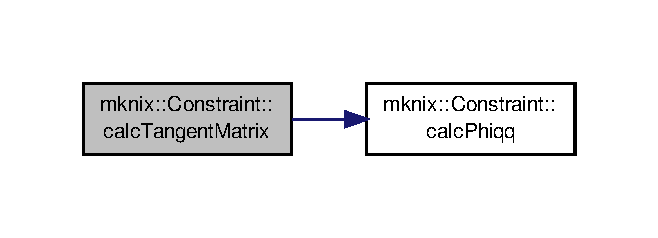
\includegraphics[width=316pt]{da/dd3/classmknix_1_1_constraint_a9b7594c65aa792ffb56d3a598996a969_cgraph}
\end{center}
\end{figure}


\hypertarget{classmknix_1_1_constraint_a26923b449734b9f11ed5ca2556585dcb}{\index{mknix\-::\-Constraint@{mknix\-::\-Constraint}!check\-Augmented@{check\-Augmented}}
\index{check\-Augmented@{check\-Augmented}!mknix::Constraint@{mknix\-::\-Constraint}}
\paragraph[{check\-Augmented}]{\setlength{\rightskip}{0pt plus 5cm}bool mknix\-::\-Constraint\-::check\-Augmented (
\begin{DoxyParamCaption}
{}
\end{DoxyParamCaption}
)\hspace{0.3cm}{\ttfamily [virtual]}}}\label{classmknix_1_1_constraint_a26923b449734b9f11ed5ca2556585dcb}
\hypertarget{classmknix_1_1_constraint_a2e1f0de7e983151fb892468774dcdf12}{\index{mknix\-::\-Constraint@{mknix\-::\-Constraint}!clear\-Augmented@{clear\-Augmented}}
\index{clear\-Augmented@{clear\-Augmented}!mknix::Constraint@{mknix\-::\-Constraint}}
\paragraph[{clear\-Augmented}]{\setlength{\rightskip}{0pt plus 5cm}void mknix\-::\-Constraint\-::clear\-Augmented (
\begin{DoxyParamCaption}
{}
\end{DoxyParamCaption}
)\hspace{0.3cm}{\ttfamily [virtual]}}}\label{classmknix_1_1_constraint_a2e1f0de7e983151fb892468774dcdf12}
\hypertarget{classmknix_1_1_constraint_a0e81d924dad26b7b5b0749d4580dd63c}{\index{mknix\-::\-Constraint@{mknix\-::\-Constraint}!get\-Node@{get\-Node}}
\index{get\-Node@{get\-Node}!mknix::Constraint@{mknix\-::\-Constraint}}
\paragraph[{get\-Node}]{\setlength{\rightskip}{0pt plus 5cm}virtual {\bf Node}$\ast$ mknix\-::\-Constraint\-::get\-Node (
\begin{DoxyParamCaption}
\item[{int}]{node\-Number}
\end{DoxyParamCaption}
)\hspace{0.3cm}{\ttfamily [inline]}, {\ttfamily [virtual]}}}\label{classmknix_1_1_constraint_a0e81d924dad26b7b5b0749d4580dd63c}


\subsubsection{Member Data Documentation}
\hypertarget{classmknix_1_1_constraint_ab76845f20e7a29693b9161e09074d55a}{\index{mknix\-::\-Constraint@{mknix\-::\-Constraint}!alpha@{alpha}}
\index{alpha@{alpha}!mknix::Constraint@{mknix\-::\-Constraint}}
\paragraph[{alpha}]{\setlength{\rightskip}{0pt plus 5cm}double mknix\-::\-Constraint\-::alpha\hspace{0.3cm}{\ttfamily [protected]}}}\label{classmknix_1_1_constraint_ab76845f20e7a29693b9161e09074d55a}
\hypertarget{classmknix_1_1_constraint_a5fa3727603b390206e6431141b892517}{\index{mknix\-::\-Constraint@{mknix\-::\-Constraint}!dim@{dim}}
\index{dim@{dim}!mknix::Constraint@{mknix\-::\-Constraint}}
\paragraph[{dim}]{\setlength{\rightskip}{0pt plus 5cm}int mknix\-::\-Constraint\-::dim\hspace{0.3cm}{\ttfamily [protected]}}}\label{classmknix_1_1_constraint_a5fa3727603b390206e6431141b892517}
\hypertarget{classmknix_1_1_constraint_a0b0fbbf149c32ce0a9dd6e0c4dd5851e}{\index{mknix\-::\-Constraint@{mknix\-::\-Constraint}!internal\-Forces@{internal\-Forces}}
\index{internal\-Forces@{internal\-Forces}!mknix::Constraint@{mknix\-::\-Constraint}}
\paragraph[{internal\-Forces}]{\setlength{\rightskip}{0pt plus 5cm}lmx\-::\-Vector$<${\bf data\-\_\-type}$>$ mknix\-::\-Constraint\-::internal\-Forces\hspace{0.3cm}{\ttfamily [protected]}}}\label{classmknix_1_1_constraint_a0b0fbbf149c32ce0a9dd6e0c4dd5851e}
\hypertarget{classmknix_1_1_constraint_aeee7c3bdd61194e3df0e958ff237040a}{\index{mknix\-::\-Constraint@{mknix\-::\-Constraint}!lambda@{lambda}}
\index{lambda@{lambda}!mknix::Constraint@{mknix\-::\-Constraint}}
\paragraph[{lambda}]{\setlength{\rightskip}{0pt plus 5cm}std\-::vector$<$ double $>$ mknix\-::\-Constraint\-::lambda\hspace{0.3cm}{\ttfamily [protected]}}}\label{classmknix_1_1_constraint_aeee7c3bdd61194e3df0e958ff237040a}
\hypertarget{classmknix_1_1_constraint_ab05c0dcc5cc535f4e3bed2fd34ed6d75}{\index{mknix\-::\-Constraint@{mknix\-::\-Constraint}!method@{method}}
\index{method@{method}!mknix::Constraint@{mknix\-::\-Constraint}}
\paragraph[{method}]{\setlength{\rightskip}{0pt plus 5cm}std\-::string mknix\-::\-Constraint\-::method\hspace{0.3cm}{\ttfamily [protected]}}}\label{classmknix_1_1_constraint_ab05c0dcc5cc535f4e3bed2fd34ed6d75}
\hypertarget{classmknix_1_1_constraint_aa4aa16e121963acf4c086f63137d4ac1}{\index{mknix\-::\-Constraint@{mknix\-::\-Constraint}!nodes@{nodes}}
\index{nodes@{nodes}!mknix::Constraint@{mknix\-::\-Constraint}}
\paragraph[{nodes}]{\setlength{\rightskip}{0pt plus 5cm}std\-::vector$<${\bf Node}$\ast$$>$ mknix\-::\-Constraint\-::nodes\hspace{0.3cm}{\ttfamily [protected]}}}\label{classmknix_1_1_constraint_aa4aa16e121963acf4c086f63137d4ac1}
\hypertarget{classmknix_1_1_constraint_a10e027fc12cb248a49a1ded049f0a161}{\index{mknix\-::\-Constraint@{mknix\-::\-Constraint}!phi@{phi}}
\index{phi@{phi}!mknix::Constraint@{mknix\-::\-Constraint}}
\paragraph[{phi}]{\setlength{\rightskip}{0pt plus 5cm}std\-::vector$<$ double $>$ mknix\-::\-Constraint\-::phi\hspace{0.3cm}{\ttfamily [protected]}}}\label{classmknix_1_1_constraint_a10e027fc12cb248a49a1ded049f0a161}
\hypertarget{classmknix_1_1_constraint_a667ecb78177b06981c30e23cb194b806}{\index{mknix\-::\-Constraint@{mknix\-::\-Constraint}!phi\-\_\-q@{phi\-\_\-q}}
\index{phi\-\_\-q@{phi\-\_\-q}!mknix::Constraint@{mknix\-::\-Constraint}}
\paragraph[{phi\-\_\-q}]{\setlength{\rightskip}{0pt plus 5cm}std\-::vector$<$ lmx\-::\-Vector$<${\bf data\-\_\-type}$>$ $>$ mknix\-::\-Constraint\-::phi\-\_\-q\hspace{0.3cm}{\ttfamily [protected]}}}\label{classmknix_1_1_constraint_a667ecb78177b06981c30e23cb194b806}
\hypertarget{classmknix_1_1_constraint_a9173b52da189652951ce51b1d69fcde4}{\index{mknix\-::\-Constraint@{mknix\-::\-Constraint}!phi\-\_\-qq@{phi\-\_\-qq}}
\index{phi\-\_\-qq@{phi\-\_\-qq}!mknix::Constraint@{mknix\-::\-Constraint}}
\paragraph[{phi\-\_\-qq}]{\setlength{\rightskip}{0pt plus 5cm}std\-::vector$<$ lmx\-::\-Dense\-Matrix$<${\bf data\-\_\-type}$>$ $>$ mknix\-::\-Constraint\-::phi\-\_\-qq\hspace{0.3cm}{\ttfamily [protected]}}}\label{classmknix_1_1_constraint_a9173b52da189652951ce51b1d69fcde4}
\hypertarget{classmknix_1_1_constraint_ab4b508cdbea36124b925f52525a1d5ad}{\index{mknix\-::\-Constraint@{mknix\-::\-Constraint}!stiffness\-Matrix@{stiffness\-Matrix}}
\index{stiffness\-Matrix@{stiffness\-Matrix}!mknix::Constraint@{mknix\-::\-Constraint}}
\paragraph[{stiffness\-Matrix}]{\setlength{\rightskip}{0pt plus 5cm}lmx\-::\-Dense\-Matrix$<${\bf data\-\_\-type}$>$ mknix\-::\-Constraint\-::stiffness\-Matrix\hspace{0.3cm}{\ttfamily [protected]}}}\label{classmknix_1_1_constraint_ab4b508cdbea36124b925f52525a1d5ad}


The documentation for this class was generated from the following files\-:\begin{DoxyCompactItemize}
\item 
\hyperlink{constraint_8h}{constraint.\-h}\item 
\hyperlink{constraint_8cpp}{constraint.\-cpp}\end{DoxyCompactItemize}

\hypertarget{classmknix_1_1_constraint_clearance}{\subsection{mknix\-:\-:Constraint\-Clearance Class Reference}
\label{classmknix_1_1_constraint_clearance}\index{mknix\-::\-Constraint\-Clearance@{mknix\-::\-Constraint\-Clearance}}
}


{\ttfamily \#include $<$constraintclearance.\-h$>$}



Inheritance diagram for mknix\-:\-:Constraint\-Clearance\-:\nopagebreak
\begin{figure}[H]
\begin{center}
\leavevmode
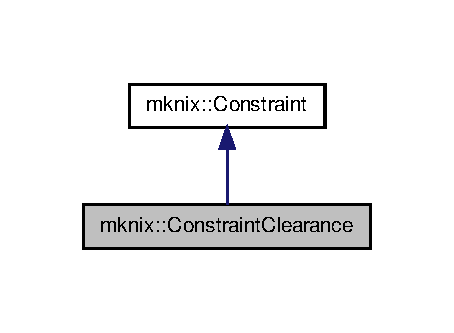
\includegraphics[width=218pt]{df/d57/classmknix_1_1_constraint_clearance__inherit__graph}
\end{center}
\end{figure}


Collaboration diagram for mknix\-:\-:Constraint\-Clearance\-:\nopagebreak
\begin{figure}[H]
\begin{center}
\leavevmode
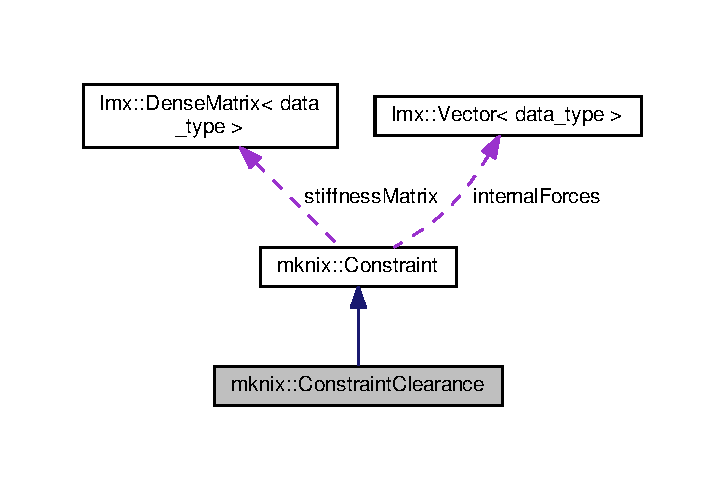
\includegraphics[width=218pt]{de/d1a/classmknix_1_1_constraint_clearance__coll__graph}
\end{center}
\end{figure}
\subsubsection*{Public Member Functions}
\begin{DoxyCompactItemize}
\item 
\hyperlink{classmknix_1_1_constraint_clearance_ad240e0d99967997aa4c2a5697aa4cb94}{Constraint\-Clearance} ()
\item 
\hyperlink{classmknix_1_1_constraint_clearance_a1db613ec74403b647fbeb68c91510c50}{$\sim$\-Constraint\-Clearance} ()
\item 
\hyperlink{classmknix_1_1_constraint_clearance_afcf63dc9c275d3ca6c55d072b2b554a2}{Constraint\-Clearance} (\hyperlink{classmknix_1_1_node}{Node} $\ast$, \hyperlink{classmknix_1_1_node}{Node} $\ast$, double \&, double \&, std\-::string \&)
\item 
void \hyperlink{classmknix_1_1_constraint_clearance_adeab95be15eee6fe28f09fafd4f5757a}{calc\-Phi} ()
\item 
void \hyperlink{classmknix_1_1_constraint_clearance_a7e834e62ef642f4f5207f3021f11020e}{calc\-Phiq} ()
\item 
void \hyperlink{classmknix_1_1_constraint_clearance_aea75fa1da7455bbefb5ce7705a16a3cc}{calc\-Phiqq} ()
\item 
lmx\-::\-Vector$<$ \hyperlink{namespacemknix_a16be4b246fbf2cceb141e3a179111020}{data\-\_\-type} $>$ \& \hyperlink{classmknix_1_1_constraint_clearance_ac190c9f0a3b0851681c6be643cb385ac}{get\-Internal\-Forces} ()
\item 
lmx\-::\-Dense\-Matrix$<$ \hyperlink{namespacemknix_a16be4b246fbf2cceb141e3a179111020}{data\-\_\-type} $>$ \& \hyperlink{classmknix_1_1_constraint_clearance_a40ac23ffea02a1a45e4b084bcd807a51}{get\-Stiffness\-Matrix} ()
\end{DoxyCompactItemize}
\subsubsection*{Protected Attributes}
\begin{DoxyCompactItemize}
\item 
double \hyperlink{classmknix_1_1_constraint_clearance_ad4bba99aa716d1f15bd9dc613f0352e8}{rh}
\item 
double \hyperlink{classmknix_1_1_constraint_clearance_a07e6a50d3416e2265e2dadb1bf730c43}{rt}
\end{DoxyCompactItemize}


\subsubsection{Detailed Description}
\begin{DoxyAuthor}{Author}
A\-U\-T\-H\-O\-R\-S $<$\-M\-A\-I\-L\-S$>$ 
\end{DoxyAuthor}


\subsubsection{Constructor \& Destructor Documentation}
\hypertarget{classmknix_1_1_constraint_clearance_ad240e0d99967997aa4c2a5697aa4cb94}{\index{mknix\-::\-Constraint\-Clearance@{mknix\-::\-Constraint\-Clearance}!Constraint\-Clearance@{Constraint\-Clearance}}
\index{Constraint\-Clearance@{Constraint\-Clearance}!mknix::ConstraintClearance@{mknix\-::\-Constraint\-Clearance}}
\paragraph[{Constraint\-Clearance}]{\setlength{\rightskip}{0pt plus 5cm}mknix\-::\-Constraint\-Clearance\-::\-Constraint\-Clearance (
\begin{DoxyParamCaption}
{}
\end{DoxyParamCaption}
)}}\label{classmknix_1_1_constraint_clearance_ad240e0d99967997aa4c2a5697aa4cb94}
\hypertarget{classmknix_1_1_constraint_clearance_a1db613ec74403b647fbeb68c91510c50}{\index{mknix\-::\-Constraint\-Clearance@{mknix\-::\-Constraint\-Clearance}!$\sim$\-Constraint\-Clearance@{$\sim$\-Constraint\-Clearance}}
\index{$\sim$\-Constraint\-Clearance@{$\sim$\-Constraint\-Clearance}!mknix::ConstraintClearance@{mknix\-::\-Constraint\-Clearance}}
\paragraph[{$\sim$\-Constraint\-Clearance}]{\setlength{\rightskip}{0pt plus 5cm}mknix\-::\-Constraint\-Clearance\-::$\sim$\-Constraint\-Clearance (
\begin{DoxyParamCaption}
{}
\end{DoxyParamCaption}
)}}\label{classmknix_1_1_constraint_clearance_a1db613ec74403b647fbeb68c91510c50}
\hypertarget{classmknix_1_1_constraint_clearance_afcf63dc9c275d3ca6c55d072b2b554a2}{\index{mknix\-::\-Constraint\-Clearance@{mknix\-::\-Constraint\-Clearance}!Constraint\-Clearance@{Constraint\-Clearance}}
\index{Constraint\-Clearance@{Constraint\-Clearance}!mknix::ConstraintClearance@{mknix\-::\-Constraint\-Clearance}}
\paragraph[{Constraint\-Clearance}]{\setlength{\rightskip}{0pt plus 5cm}mknix\-::\-Constraint\-Clearance\-::\-Constraint\-Clearance (
\begin{DoxyParamCaption}
\item[{{\bf Node} $\ast$}]{a\-\_\-in, }
\item[{{\bf Node} $\ast$}]{b\-\_\-in, }
\item[{double \&}]{rh\-\_\-in, }
\item[{double \&}]{alpha\-\_\-in, }
\item[{std\-::string \&}]{method\-\_\-in}
\end{DoxyParamCaption}
)}}\label{classmknix_1_1_constraint_clearance_afcf63dc9c275d3ca6c55d072b2b554a2}


\subsubsection{Member Function Documentation}
\hypertarget{classmknix_1_1_constraint_clearance_adeab95be15eee6fe28f09fafd4f5757a}{\index{mknix\-::\-Constraint\-Clearance@{mknix\-::\-Constraint\-Clearance}!calc\-Phi@{calc\-Phi}}
\index{calc\-Phi@{calc\-Phi}!mknix::ConstraintClearance@{mknix\-::\-Constraint\-Clearance}}
\paragraph[{calc\-Phi}]{\setlength{\rightskip}{0pt plus 5cm}void mknix\-::\-Constraint\-Clearance\-::calc\-Phi (
\begin{DoxyParamCaption}
{}
\end{DoxyParamCaption}
)\hspace{0.3cm}{\ttfamily [virtual]}}}\label{classmknix_1_1_constraint_clearance_adeab95be15eee6fe28f09fafd4f5757a}


Implements \hyperlink{classmknix_1_1_constraint_a7f2b34d256d5eec54b34b0440b562ec1}{mknix\-::\-Constraint}.

\hypertarget{classmknix_1_1_constraint_clearance_a7e834e62ef642f4f5207f3021f11020e}{\index{mknix\-::\-Constraint\-Clearance@{mknix\-::\-Constraint\-Clearance}!calc\-Phiq@{calc\-Phiq}}
\index{calc\-Phiq@{calc\-Phiq}!mknix::ConstraintClearance@{mknix\-::\-Constraint\-Clearance}}
\paragraph[{calc\-Phiq}]{\setlength{\rightskip}{0pt plus 5cm}void mknix\-::\-Constraint\-Clearance\-::calc\-Phiq (
\begin{DoxyParamCaption}
{}
\end{DoxyParamCaption}
)\hspace{0.3cm}{\ttfamily [virtual]}}}\label{classmknix_1_1_constraint_clearance_a7e834e62ef642f4f5207f3021f11020e}


Implements \hyperlink{classmknix_1_1_constraint_ab129143960df2b9459e274275608bcf2}{mknix\-::\-Constraint}.

\hypertarget{classmknix_1_1_constraint_clearance_aea75fa1da7455bbefb5ce7705a16a3cc}{\index{mknix\-::\-Constraint\-Clearance@{mknix\-::\-Constraint\-Clearance}!calc\-Phiqq@{calc\-Phiqq}}
\index{calc\-Phiqq@{calc\-Phiqq}!mknix::ConstraintClearance@{mknix\-::\-Constraint\-Clearance}}
\paragraph[{calc\-Phiqq}]{\setlength{\rightskip}{0pt plus 5cm}void mknix\-::\-Constraint\-Clearance\-::calc\-Phiqq (
\begin{DoxyParamCaption}
{}
\end{DoxyParamCaption}
)\hspace{0.3cm}{\ttfamily [virtual]}}}\label{classmknix_1_1_constraint_clearance_aea75fa1da7455bbefb5ce7705a16a3cc}


Implements \hyperlink{classmknix_1_1_constraint_a73ff21573b5e9c4acda789bd5ac46ea8}{mknix\-::\-Constraint}.

\hypertarget{classmknix_1_1_constraint_clearance_ac190c9f0a3b0851681c6be643cb385ac}{\index{mknix\-::\-Constraint\-Clearance@{mknix\-::\-Constraint\-Clearance}!get\-Internal\-Forces@{get\-Internal\-Forces}}
\index{get\-Internal\-Forces@{get\-Internal\-Forces}!mknix::ConstraintClearance@{mknix\-::\-Constraint\-Clearance}}
\paragraph[{get\-Internal\-Forces}]{\setlength{\rightskip}{0pt plus 5cm}lmx\-::\-Vector$<${\bf data\-\_\-type}$>$\& mknix\-::\-Constraint\-Clearance\-::get\-Internal\-Forces (
\begin{DoxyParamCaption}
{}
\end{DoxyParamCaption}
)\hspace{0.3cm}{\ttfamily [inline]}}}\label{classmknix_1_1_constraint_clearance_ac190c9f0a3b0851681c6be643cb385ac}
\hypertarget{classmknix_1_1_constraint_clearance_a40ac23ffea02a1a45e4b084bcd807a51}{\index{mknix\-::\-Constraint\-Clearance@{mknix\-::\-Constraint\-Clearance}!get\-Stiffness\-Matrix@{get\-Stiffness\-Matrix}}
\index{get\-Stiffness\-Matrix@{get\-Stiffness\-Matrix}!mknix::ConstraintClearance@{mknix\-::\-Constraint\-Clearance}}
\paragraph[{get\-Stiffness\-Matrix}]{\setlength{\rightskip}{0pt plus 5cm}lmx\-::\-Dense\-Matrix$<${\bf data\-\_\-type}$>$\& mknix\-::\-Constraint\-Clearance\-::get\-Stiffness\-Matrix (
\begin{DoxyParamCaption}
{}
\end{DoxyParamCaption}
)\hspace{0.3cm}{\ttfamily [inline]}}}\label{classmknix_1_1_constraint_clearance_a40ac23ffea02a1a45e4b084bcd807a51}


\subsubsection{Member Data Documentation}
\hypertarget{classmknix_1_1_constraint_clearance_ad4bba99aa716d1f15bd9dc613f0352e8}{\index{mknix\-::\-Constraint\-Clearance@{mknix\-::\-Constraint\-Clearance}!rh@{rh}}
\index{rh@{rh}!mknix::ConstraintClearance@{mknix\-::\-Constraint\-Clearance}}
\paragraph[{rh}]{\setlength{\rightskip}{0pt plus 5cm}double mknix\-::\-Constraint\-Clearance\-::rh\hspace{0.3cm}{\ttfamily [protected]}}}\label{classmknix_1_1_constraint_clearance_ad4bba99aa716d1f15bd9dc613f0352e8}
\hypertarget{classmknix_1_1_constraint_clearance_a07e6a50d3416e2265e2dadb1bf730c43}{\index{mknix\-::\-Constraint\-Clearance@{mknix\-::\-Constraint\-Clearance}!rt@{rt}}
\index{rt@{rt}!mknix::ConstraintClearance@{mknix\-::\-Constraint\-Clearance}}
\paragraph[{rt}]{\setlength{\rightskip}{0pt plus 5cm}double mknix\-::\-Constraint\-Clearance\-::rt\hspace{0.3cm}{\ttfamily [protected]}}}\label{classmknix_1_1_constraint_clearance_a07e6a50d3416e2265e2dadb1bf730c43}


The documentation for this class was generated from the following files\-:\begin{DoxyCompactItemize}
\item 
\hyperlink{constraintclearance_8h}{constraintclearance.\-h}\item 
\hyperlink{constraintclearance_8cpp}{constraintclearance.\-cpp}\end{DoxyCompactItemize}

\hypertarget{classmknix_1_1_constraint_contact}{\subsection{mknix\-:\-:Constraint\-Contact Class Reference}
\label{classmknix_1_1_constraint_contact}\index{mknix\-::\-Constraint\-Contact@{mknix\-::\-Constraint\-Contact}}
}


{\ttfamily \#include $<$constraintcontact.\-h$>$}



Inheritance diagram for mknix\-:\-:Constraint\-Contact\-:\nopagebreak
\begin{figure}[H]
\begin{center}
\leavevmode
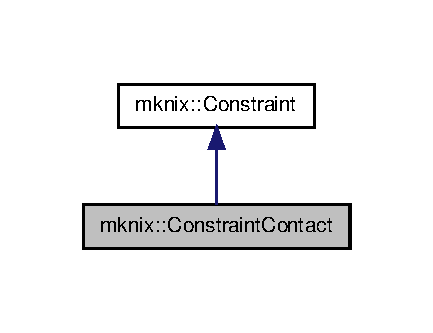
\includegraphics[width=208pt]{d2/d65/classmknix_1_1_constraint_contact__inherit__graph}
\end{center}
\end{figure}


Collaboration diagram for mknix\-:\-:Constraint\-Contact\-:\nopagebreak
\begin{figure}[H]
\begin{center}
\leavevmode
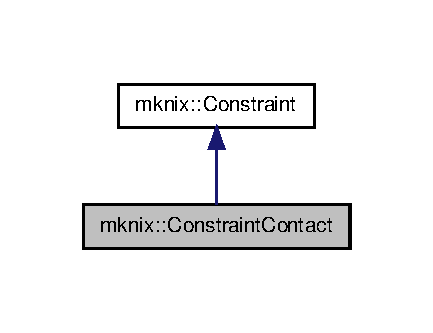
\includegraphics[width=208pt]{d1/d4f/classmknix_1_1_constraint_contact__coll__graph}
\end{center}
\end{figure}
\subsubsection*{Public Member Functions}
\begin{DoxyCompactItemize}
\item 
\hyperlink{classmknix_1_1_constraint_contact_a76498ab5af03df8fd8c850f67ac54d33}{Constraint\-Contact} ()
\item 
\hyperlink{classmknix_1_1_constraint_contact_a2570dc3ad5c593871f1d5dd4e6302f07}{$\sim$\-Constraint\-Contact} ()
\item 
\hyperlink{classmknix_1_1_constraint_contact_abfcda7ac9dc63a790078f2fb26497a6e}{Constraint\-Contact} (\hyperlink{classmknix_1_1_node}{Node} $\ast$, \hyperlink{classmknix_1_1_node}{Node} $\ast$, \hyperlink{classmknix_1_1_node}{Node} $\ast$, double \&, std\-::string \&)
\item 
void \hyperlink{classmknix_1_1_constraint_contact_a21a89037754ef5d968bda199ad3f1858}{calc\-Phi} ()
\item 
void \hyperlink{classmknix_1_1_constraint_contact_a88c495ea01a5f8f8807dd72ae3e7240f}{calc\-Phiq} ()
\item 
void \hyperlink{classmknix_1_1_constraint_contact_ad9b4db34bf76f2d8ea9532d5d3e0449f}{calc\-Phiqq} ()
\item 
lmx\-::\-Vector$<$ \hyperlink{namespacemknix_a16be4b246fbf2cceb141e3a179111020}{data\-\_\-type} $>$ \& \hyperlink{classmknix_1_1_constraint_contact_ae4ebea11a39b4cf89ce317154abc99e3}{get\-Internal\-Forces} ()
\item 
lmx\-::\-Dense\-Matrix$<$ \hyperlink{namespacemknix_a16be4b246fbf2cceb141e3a179111020}{data\-\_\-type} $>$ \& \hyperlink{classmknix_1_1_constraint_contact_abb4cb7497d2cbef540add289fdf8492e}{get\-Stiffness\-Matrix} ()
\item 
double \hyperlink{classmknix_1_1_constraint_contact_a4fcfe47c1421fd375ff806b8ef411f47}{get\-Gap} ()
\end{DoxyCompactItemize}
\subsubsection*{Protected Attributes}
\begin{DoxyCompactItemize}
\item 
std\-::vector$<$ double $>$ \hyperlink{classmknix_1_1_constraint_contact_a06ba5460d950b98b85226e7b9b520df2}{normal}
\item 
double \hyperlink{classmknix_1_1_constraint_contact_a86b0413ea70c74a38f8610a88cba48c6}{rh}
\item 
double \hyperlink{classmknix_1_1_constraint_contact_a0a2b6bbee4925e12f4921aa58f0f3426}{rt}
\end{DoxyCompactItemize}


\subsubsection{Detailed Description}
\begin{DoxyAuthor}{Author}
A\-U\-T\-H\-O\-R\-S $<$\-M\-A\-I\-L\-S$>$ 
\end{DoxyAuthor}


\subsubsection{Constructor \& Destructor Documentation}
\hypertarget{classmknix_1_1_constraint_contact_a76498ab5af03df8fd8c850f67ac54d33}{\index{mknix\-::\-Constraint\-Contact@{mknix\-::\-Constraint\-Contact}!Constraint\-Contact@{Constraint\-Contact}}
\index{Constraint\-Contact@{Constraint\-Contact}!mknix::ConstraintContact@{mknix\-::\-Constraint\-Contact}}
\paragraph[{Constraint\-Contact}]{\setlength{\rightskip}{0pt plus 5cm}mknix\-::\-Constraint\-Contact\-::\-Constraint\-Contact (
\begin{DoxyParamCaption}
{}
\end{DoxyParamCaption}
)}}\label{classmknix_1_1_constraint_contact_a76498ab5af03df8fd8c850f67ac54d33}
\hypertarget{classmknix_1_1_constraint_contact_a2570dc3ad5c593871f1d5dd4e6302f07}{\index{mknix\-::\-Constraint\-Contact@{mknix\-::\-Constraint\-Contact}!$\sim$\-Constraint\-Contact@{$\sim$\-Constraint\-Contact}}
\index{$\sim$\-Constraint\-Contact@{$\sim$\-Constraint\-Contact}!mknix::ConstraintContact@{mknix\-::\-Constraint\-Contact}}
\paragraph[{$\sim$\-Constraint\-Contact}]{\setlength{\rightskip}{0pt plus 5cm}mknix\-::\-Constraint\-Contact\-::$\sim$\-Constraint\-Contact (
\begin{DoxyParamCaption}
{}
\end{DoxyParamCaption}
)}}\label{classmknix_1_1_constraint_contact_a2570dc3ad5c593871f1d5dd4e6302f07}
\hypertarget{classmknix_1_1_constraint_contact_abfcda7ac9dc63a790078f2fb26497a6e}{\index{mknix\-::\-Constraint\-Contact@{mknix\-::\-Constraint\-Contact}!Constraint\-Contact@{Constraint\-Contact}}
\index{Constraint\-Contact@{Constraint\-Contact}!mknix::ConstraintContact@{mknix\-::\-Constraint\-Contact}}
\paragraph[{Constraint\-Contact}]{\setlength{\rightskip}{0pt plus 5cm}mknix\-::\-Constraint\-Contact\-::\-Constraint\-Contact (
\begin{DoxyParamCaption}
\item[{{\bf Node} $\ast$}]{q1\-\_\-in, }
\item[{{\bf Node} $\ast$}]{q2\-\_\-in, }
\item[{{\bf Node} $\ast$}]{p\-\_\-in, }
\item[{double \&}]{alpha\-\_\-in, }
\item[{std\-::string \&}]{method\-\_\-in}
\end{DoxyParamCaption}
)}}\label{classmknix_1_1_constraint_contact_abfcda7ac9dc63a790078f2fb26497a6e}


\subsubsection{Member Function Documentation}
\hypertarget{classmknix_1_1_constraint_contact_a21a89037754ef5d968bda199ad3f1858}{\index{mknix\-::\-Constraint\-Contact@{mknix\-::\-Constraint\-Contact}!calc\-Phi@{calc\-Phi}}
\index{calc\-Phi@{calc\-Phi}!mknix::ConstraintContact@{mknix\-::\-Constraint\-Contact}}
\paragraph[{calc\-Phi}]{\setlength{\rightskip}{0pt plus 5cm}void mknix\-::\-Constraint\-Contact\-::calc\-Phi (
\begin{DoxyParamCaption}
{}
\end{DoxyParamCaption}
)\hspace{0.3cm}{\ttfamily [virtual]}}}\label{classmknix_1_1_constraint_contact_a21a89037754ef5d968bda199ad3f1858}


Implements \hyperlink{classmknix_1_1_constraint_a7f2b34d256d5eec54b34b0440b562ec1}{mknix\-::\-Constraint}.

\hypertarget{classmknix_1_1_constraint_contact_a88c495ea01a5f8f8807dd72ae3e7240f}{\index{mknix\-::\-Constraint\-Contact@{mknix\-::\-Constraint\-Contact}!calc\-Phiq@{calc\-Phiq}}
\index{calc\-Phiq@{calc\-Phiq}!mknix::ConstraintContact@{mknix\-::\-Constraint\-Contact}}
\paragraph[{calc\-Phiq}]{\setlength{\rightskip}{0pt plus 5cm}void mknix\-::\-Constraint\-Contact\-::calc\-Phiq (
\begin{DoxyParamCaption}
{}
\end{DoxyParamCaption}
)\hspace{0.3cm}{\ttfamily [virtual]}}}\label{classmknix_1_1_constraint_contact_a88c495ea01a5f8f8807dd72ae3e7240f}


Implements \hyperlink{classmknix_1_1_constraint_ab129143960df2b9459e274275608bcf2}{mknix\-::\-Constraint}.

\hypertarget{classmknix_1_1_constraint_contact_ad9b4db34bf76f2d8ea9532d5d3e0449f}{\index{mknix\-::\-Constraint\-Contact@{mknix\-::\-Constraint\-Contact}!calc\-Phiqq@{calc\-Phiqq}}
\index{calc\-Phiqq@{calc\-Phiqq}!mknix::ConstraintContact@{mknix\-::\-Constraint\-Contact}}
\paragraph[{calc\-Phiqq}]{\setlength{\rightskip}{0pt plus 5cm}void mknix\-::\-Constraint\-Contact\-::calc\-Phiqq (
\begin{DoxyParamCaption}
{}
\end{DoxyParamCaption}
)\hspace{0.3cm}{\ttfamily [virtual]}}}\label{classmknix_1_1_constraint_contact_ad9b4db34bf76f2d8ea9532d5d3e0449f}


Implements \hyperlink{classmknix_1_1_constraint_a73ff21573b5e9c4acda789bd5ac46ea8}{mknix\-::\-Constraint}.

\hypertarget{classmknix_1_1_constraint_contact_a4fcfe47c1421fd375ff806b8ef411f47}{\index{mknix\-::\-Constraint\-Contact@{mknix\-::\-Constraint\-Contact}!get\-Gap@{get\-Gap}}
\index{get\-Gap@{get\-Gap}!mknix::ConstraintContact@{mknix\-::\-Constraint\-Contact}}
\paragraph[{get\-Gap}]{\setlength{\rightskip}{0pt plus 5cm}double mknix\-::\-Constraint\-Contact\-::get\-Gap (
\begin{DoxyParamCaption}
{}
\end{DoxyParamCaption}
)\hspace{0.3cm}{\ttfamily [inline]}}}\label{classmknix_1_1_constraint_contact_a4fcfe47c1421fd375ff806b8ef411f47}
\hypertarget{classmknix_1_1_constraint_contact_ae4ebea11a39b4cf89ce317154abc99e3}{\index{mknix\-::\-Constraint\-Contact@{mknix\-::\-Constraint\-Contact}!get\-Internal\-Forces@{get\-Internal\-Forces}}
\index{get\-Internal\-Forces@{get\-Internal\-Forces}!mknix::ConstraintContact@{mknix\-::\-Constraint\-Contact}}
\paragraph[{get\-Internal\-Forces}]{\setlength{\rightskip}{0pt plus 5cm}lmx\-::\-Vector$<${\bf data\-\_\-type}$>$\& mknix\-::\-Constraint\-Contact\-::get\-Internal\-Forces (
\begin{DoxyParamCaption}
{}
\end{DoxyParamCaption}
)\hspace{0.3cm}{\ttfamily [inline]}}}\label{classmknix_1_1_constraint_contact_ae4ebea11a39b4cf89ce317154abc99e3}
\hypertarget{classmknix_1_1_constraint_contact_abb4cb7497d2cbef540add289fdf8492e}{\index{mknix\-::\-Constraint\-Contact@{mknix\-::\-Constraint\-Contact}!get\-Stiffness\-Matrix@{get\-Stiffness\-Matrix}}
\index{get\-Stiffness\-Matrix@{get\-Stiffness\-Matrix}!mknix::ConstraintContact@{mknix\-::\-Constraint\-Contact}}
\paragraph[{get\-Stiffness\-Matrix}]{\setlength{\rightskip}{0pt plus 5cm}lmx\-::\-Dense\-Matrix$<${\bf data\-\_\-type}$>$\& mknix\-::\-Constraint\-Contact\-::get\-Stiffness\-Matrix (
\begin{DoxyParamCaption}
{}
\end{DoxyParamCaption}
)\hspace{0.3cm}{\ttfamily [inline]}}}\label{classmknix_1_1_constraint_contact_abb4cb7497d2cbef540add289fdf8492e}


\subsubsection{Member Data Documentation}
\hypertarget{classmknix_1_1_constraint_contact_a06ba5460d950b98b85226e7b9b520df2}{\index{mknix\-::\-Constraint\-Contact@{mknix\-::\-Constraint\-Contact}!normal@{normal}}
\index{normal@{normal}!mknix::ConstraintContact@{mknix\-::\-Constraint\-Contact}}
\paragraph[{normal}]{\setlength{\rightskip}{0pt plus 5cm}std\-::vector$<$double$>$ mknix\-::\-Constraint\-Contact\-::normal\hspace{0.3cm}{\ttfamily [protected]}}}\label{classmknix_1_1_constraint_contact_a06ba5460d950b98b85226e7b9b520df2}
\hypertarget{classmknix_1_1_constraint_contact_a86b0413ea70c74a38f8610a88cba48c6}{\index{mknix\-::\-Constraint\-Contact@{mknix\-::\-Constraint\-Contact}!rh@{rh}}
\index{rh@{rh}!mknix::ConstraintContact@{mknix\-::\-Constraint\-Contact}}
\paragraph[{rh}]{\setlength{\rightskip}{0pt plus 5cm}double mknix\-::\-Constraint\-Contact\-::rh\hspace{0.3cm}{\ttfamily [protected]}}}\label{classmknix_1_1_constraint_contact_a86b0413ea70c74a38f8610a88cba48c6}
\hypertarget{classmknix_1_1_constraint_contact_a0a2b6bbee4925e12f4921aa58f0f3426}{\index{mknix\-::\-Constraint\-Contact@{mknix\-::\-Constraint\-Contact}!rt@{rt}}
\index{rt@{rt}!mknix::ConstraintContact@{mknix\-::\-Constraint\-Contact}}
\paragraph[{rt}]{\setlength{\rightskip}{0pt plus 5cm}double mknix\-::\-Constraint\-Contact\-::rt\hspace{0.3cm}{\ttfamily [protected]}}}\label{classmknix_1_1_constraint_contact_a0a2b6bbee4925e12f4921aa58f0f3426}


The documentation for this class was generated from the following files\-:\begin{DoxyCompactItemize}
\item 
\hyperlink{constraintcontact_8h}{constraintcontact.\-h}\item 
\hyperlink{constraintcontact_8cpp}{constraintcontact.\-cpp}\end{DoxyCompactItemize}

\hypertarget{classmknix_1_1_constraint_distance}{}\subsection{mknix\+:\+:Constraint\+Distance Class Reference}
\label{classmknix_1_1_constraint_distance}\index{mknix\+::\+Constraint\+Distance@{mknix\+::\+Constraint\+Distance}}


{\ttfamily \#include $<$constraintdistance.\+h$>$}



Inheritance diagram for mknix\+:\+:Constraint\+Distance\+:\nopagebreak
\begin{figure}[H]
\begin{center}
\leavevmode
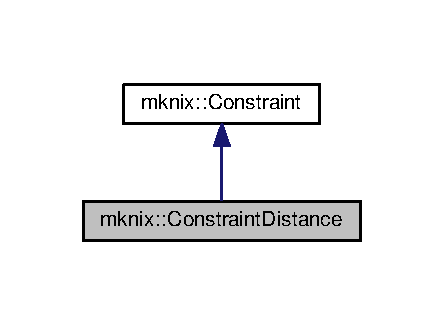
\includegraphics[width=213pt]{dd/dfd/classmknix_1_1_constraint_distance__inherit__graph}
\end{center}
\end{figure}


Collaboration diagram for mknix\+:\+:Constraint\+Distance\+:\nopagebreak
\begin{figure}[H]
\begin{center}
\leavevmode
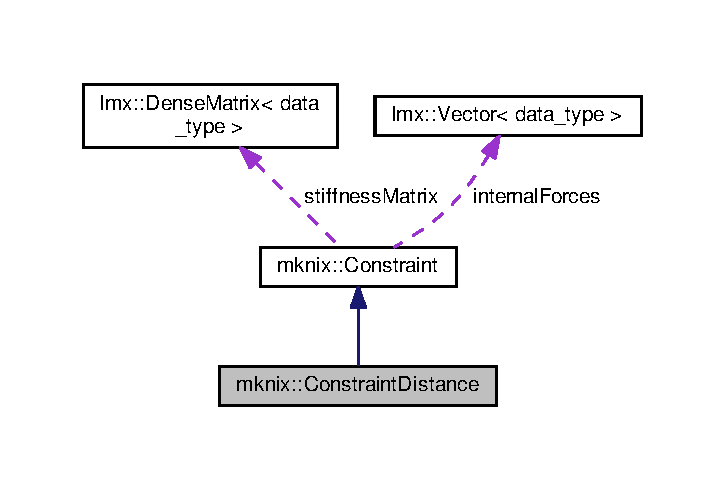
\includegraphics[width=348pt]{da/d3d/classmknix_1_1_constraint_distance__coll__graph}
\end{center}
\end{figure}
\subsubsection*{Public Member Functions}
\begin{DoxyCompactItemize}
\item 
\hyperlink{classmknix_1_1_constraint_distance_ad89b1d56b296625e72fe0bcf4cea3c5c}{Constraint\+Distance} ()
\item 
\hyperlink{classmknix_1_1_constraint_distance_aa39735f682295e2c7b839fddb9eba545}{$\sim$\+Constraint\+Distance} ()
\item 
\hyperlink{classmknix_1_1_constraint_distance_adc9113e52374f275b1b79bfdca72b971}{Constraint\+Distance} (\hyperlink{classmknix_1_1_node}{Node} $\ast$, \hyperlink{classmknix_1_1_node}{Node} $\ast$, double \&, std\+::string \&)
\item 
void \hyperlink{classmknix_1_1_constraint_distance_a32df0e5f0198ce5c7871e2b6a5cafb7c}{calc\+Ro} ()
\item 
void \hyperlink{classmknix_1_1_constraint_distance_ad838af34d5ada5ba2f4ce559a472e16a}{calc\+Phi} ()
\item 
void \hyperlink{classmknix_1_1_constraint_distance_a6fa6c37266c01a1e8f577418dd886037}{calc\+Phiq} ()
\item 
void \hyperlink{classmknix_1_1_constraint_distance_ad4d1eb206239508f7f2f5b4d26b957eb}{calc\+Phiqq} ()
\item 
void \hyperlink{classmknix_1_1_constraint_distance_aadda81ffe998ebc5d03adc91f73a016e}{set\+Lenght} (double new\+\_\+ro)
\item 
\hyperlink{classlmx_1_1_vector}{lmx\+::\+Vector}$<$ \hyperlink{namespacemknix_a16be4b246fbf2cceb141e3a179111020}{data\+\_\+type} $>$ \& \hyperlink{classmknix_1_1_constraint_distance_aae757ba28e181259a196fbc0a1e8bfaf}{get\+Internal\+Forces} ()
\item 
\hyperlink{classlmx_1_1_dense_matrix}{lmx\+::\+Dense\+Matrix}$<$ \hyperlink{namespacemknix_a16be4b246fbf2cceb141e3a179111020}{data\+\_\+type} $>$ \& \hyperlink{classmknix_1_1_constraint_distance_a847365545dcef34ee44bbadd20d819bf}{get\+Stiffness\+Matrix} ()
\end{DoxyCompactItemize}
\subsubsection*{Protected Attributes}
\begin{DoxyCompactItemize}
\item 
double \hyperlink{classmknix_1_1_constraint_distance_a2d4a4e3c3b75b23f63a772b71c4badaa}{ro}
\item 
double \hyperlink{classmknix_1_1_constraint_distance_ae4054619a2e3205079c4911ad69db4eb}{rt}
\end{DoxyCompactItemize}


\subsubsection{Detailed Description}
\begin{DoxyAuthor}{Author}
A\+U\+T\+H\+O\+R\+S $<$\+M\+A\+I\+L\+S$>$ 
\end{DoxyAuthor}


Definition at line 30 of file constraintdistance.\+h.



\subsubsection{Constructor \& Destructor Documentation}
\hypertarget{classmknix_1_1_constraint_distance_ad89b1d56b296625e72fe0bcf4cea3c5c}{}\index{mknix\+::\+Constraint\+Distance@{mknix\+::\+Constraint\+Distance}!Constraint\+Distance@{Constraint\+Distance}}
\index{Constraint\+Distance@{Constraint\+Distance}!mknix\+::\+Constraint\+Distance@{mknix\+::\+Constraint\+Distance}}
\paragraph[{Constraint\+Distance}]{\setlength{\rightskip}{0pt plus 5cm}mknix\+::\+Constraint\+Distance\+::\+Constraint\+Distance (
\begin{DoxyParamCaption}
{}
\end{DoxyParamCaption}
)}\label{classmknix_1_1_constraint_distance_ad89b1d56b296625e72fe0bcf4cea3c5c}


Definition at line 27 of file constraintdistance.\+cpp.

\hypertarget{classmknix_1_1_constraint_distance_aa39735f682295e2c7b839fddb9eba545}{}\index{mknix\+::\+Constraint\+Distance@{mknix\+::\+Constraint\+Distance}!````~Constraint\+Distance@{$\sim$\+Constraint\+Distance}}
\index{````~Constraint\+Distance@{$\sim$\+Constraint\+Distance}!mknix\+::\+Constraint\+Distance@{mknix\+::\+Constraint\+Distance}}
\paragraph[{$\sim$\+Constraint\+Distance}]{\setlength{\rightskip}{0pt plus 5cm}mknix\+::\+Constraint\+Distance\+::$\sim$\+Constraint\+Distance (
\begin{DoxyParamCaption}
{}
\end{DoxyParamCaption}
)}\label{classmknix_1_1_constraint_distance_aa39735f682295e2c7b839fddb9eba545}


Definition at line 60 of file constraintdistance.\+cpp.

\hypertarget{classmknix_1_1_constraint_distance_adc9113e52374f275b1b79bfdca72b971}{}\index{mknix\+::\+Constraint\+Distance@{mknix\+::\+Constraint\+Distance}!Constraint\+Distance@{Constraint\+Distance}}
\index{Constraint\+Distance@{Constraint\+Distance}!mknix\+::\+Constraint\+Distance@{mknix\+::\+Constraint\+Distance}}
\paragraph[{Constraint\+Distance}]{\setlength{\rightskip}{0pt plus 5cm}mknix\+::\+Constraint\+Distance\+::\+Constraint\+Distance (
\begin{DoxyParamCaption}
\item[{{\bf Node} $\ast$}]{a\+\_\+in, }
\item[{{\bf Node} $\ast$}]{b\+\_\+in, }
\item[{double \&}]{alpha\+\_\+in, }
\item[{std\+::string \&}]{method\+\_\+in}
\end{DoxyParamCaption}
)}\label{classmknix_1_1_constraint_distance_adc9113e52374f275b1b79bfdca72b971}


Definition at line 32 of file constraintdistance.\+cpp.



Here is the call graph for this function\+:\nopagebreak
\begin{figure}[H]
\begin{center}
\leavevmode
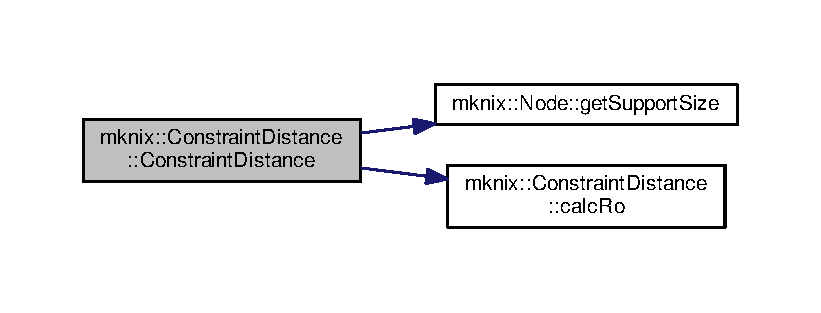
\includegraphics[width=350pt]{d7/de2/classmknix_1_1_constraint_distance_adc9113e52374f275b1b79bfdca72b971_cgraph}
\end{center}
\end{figure}




\subsubsection{Member Function Documentation}
\hypertarget{classmknix_1_1_constraint_distance_ad838af34d5ada5ba2f4ce559a472e16a}{}\index{mknix\+::\+Constraint\+Distance@{mknix\+::\+Constraint\+Distance}!calc\+Phi@{calc\+Phi}}
\index{calc\+Phi@{calc\+Phi}!mknix\+::\+Constraint\+Distance@{mknix\+::\+Constraint\+Distance}}
\paragraph[{calc\+Phi}]{\setlength{\rightskip}{0pt plus 5cm}void mknix\+::\+Constraint\+Distance\+::calc\+Phi (
\begin{DoxyParamCaption}
{}
\end{DoxyParamCaption}
)\hspace{0.3cm}{\ttfamily [virtual]}}\label{classmknix_1_1_constraint_distance_ad838af34d5ada5ba2f4ce559a472e16a}


Implements \hyperlink{classmknix_1_1_constraint_a7f2b34d256d5eec54b34b0440b562ec1}{mknix\+::\+Constraint}.



Definition at line 76 of file constraintdistance.\+cpp.

\hypertarget{classmknix_1_1_constraint_distance_a6fa6c37266c01a1e8f577418dd886037}{}\index{mknix\+::\+Constraint\+Distance@{mknix\+::\+Constraint\+Distance}!calc\+Phiq@{calc\+Phiq}}
\index{calc\+Phiq@{calc\+Phiq}!mknix\+::\+Constraint\+Distance@{mknix\+::\+Constraint\+Distance}}
\paragraph[{calc\+Phiq}]{\setlength{\rightskip}{0pt plus 5cm}void mknix\+::\+Constraint\+Distance\+::calc\+Phiq (
\begin{DoxyParamCaption}
{}
\end{DoxyParamCaption}
)\hspace{0.3cm}{\ttfamily [virtual]}}\label{classmknix_1_1_constraint_distance_a6fa6c37266c01a1e8f577418dd886037}


Implements \hyperlink{classmknix_1_1_constraint_ab129143960df2b9459e274275608bcf2}{mknix\+::\+Constraint}.



Definition at line 106 of file constraintdistance.\+cpp.

\hypertarget{classmknix_1_1_constraint_distance_ad4d1eb206239508f7f2f5b4d26b957eb}{}\index{mknix\+::\+Constraint\+Distance@{mknix\+::\+Constraint\+Distance}!calc\+Phiqq@{calc\+Phiqq}}
\index{calc\+Phiqq@{calc\+Phiqq}!mknix\+::\+Constraint\+Distance@{mknix\+::\+Constraint\+Distance}}
\paragraph[{calc\+Phiqq}]{\setlength{\rightskip}{0pt plus 5cm}void mknix\+::\+Constraint\+Distance\+::calc\+Phiqq (
\begin{DoxyParamCaption}
{}
\end{DoxyParamCaption}
)\hspace{0.3cm}{\ttfamily [virtual]}}\label{classmknix_1_1_constraint_distance_ad4d1eb206239508f7f2f5b4d26b957eb}


Implements \hyperlink{classmknix_1_1_constraint_a73ff21573b5e9c4acda789bd5ac46ea8}{mknix\+::\+Constraint}.



Definition at line 118 of file constraintdistance.\+cpp.

\hypertarget{classmknix_1_1_constraint_distance_a32df0e5f0198ce5c7871e2b6a5cafb7c}{}\index{mknix\+::\+Constraint\+Distance@{mknix\+::\+Constraint\+Distance}!calc\+Ro@{calc\+Ro}}
\index{calc\+Ro@{calc\+Ro}!mknix\+::\+Constraint\+Distance@{mknix\+::\+Constraint\+Distance}}
\paragraph[{calc\+Ro}]{\setlength{\rightskip}{0pt plus 5cm}void mknix\+::\+Constraint\+Distance\+::calc\+Ro (
\begin{DoxyParamCaption}
{}
\end{DoxyParamCaption}
)}\label{classmknix_1_1_constraint_distance_a32df0e5f0198ce5c7871e2b6a5cafb7c}


Definition at line 64 of file constraintdistance.\+cpp.



Here is the caller graph for this function\+:\nopagebreak
\begin{figure}[H]
\begin{center}
\leavevmode
\includegraphics[width=350pt]{d7/de2/classmknix_1_1_constraint_distance_a32df0e5f0198ce5c7871e2b6a5cafb7c_icgraph}
\end{center}
\end{figure}


\hypertarget{classmknix_1_1_constraint_distance_aae757ba28e181259a196fbc0a1e8bfaf}{}\index{mknix\+::\+Constraint\+Distance@{mknix\+::\+Constraint\+Distance}!get\+Internal\+Forces@{get\+Internal\+Forces}}
\index{get\+Internal\+Forces@{get\+Internal\+Forces}!mknix\+::\+Constraint\+Distance@{mknix\+::\+Constraint\+Distance}}
\paragraph[{get\+Internal\+Forces}]{\setlength{\rightskip}{0pt plus 5cm}{\bf lmx\+::\+Vector}$<${\bf data\+\_\+type}$>$\& mknix\+::\+Constraint\+Distance\+::get\+Internal\+Forces (
\begin{DoxyParamCaption}
{}
\end{DoxyParamCaption}
)\hspace{0.3cm}{\ttfamily [inline]}}\label{classmknix_1_1_constraint_distance_aae757ba28e181259a196fbc0a1e8bfaf}


Definition at line 52 of file constraintdistance.\+h.

\hypertarget{classmknix_1_1_constraint_distance_a847365545dcef34ee44bbadd20d819bf}{}\index{mknix\+::\+Constraint\+Distance@{mknix\+::\+Constraint\+Distance}!get\+Stiffness\+Matrix@{get\+Stiffness\+Matrix}}
\index{get\+Stiffness\+Matrix@{get\+Stiffness\+Matrix}!mknix\+::\+Constraint\+Distance@{mknix\+::\+Constraint\+Distance}}
\paragraph[{get\+Stiffness\+Matrix}]{\setlength{\rightskip}{0pt plus 5cm}{\bf lmx\+::\+Dense\+Matrix}$<${\bf data\+\_\+type}$>$\& mknix\+::\+Constraint\+Distance\+::get\+Stiffness\+Matrix (
\begin{DoxyParamCaption}
{}
\end{DoxyParamCaption}
)\hspace{0.3cm}{\ttfamily [inline]}}\label{classmknix_1_1_constraint_distance_a847365545dcef34ee44bbadd20d819bf}


Definition at line 56 of file constraintdistance.\+h.

\hypertarget{classmknix_1_1_constraint_distance_aadda81ffe998ebc5d03adc91f73a016e}{}\index{mknix\+::\+Constraint\+Distance@{mknix\+::\+Constraint\+Distance}!set\+Lenght@{set\+Lenght}}
\index{set\+Lenght@{set\+Lenght}!mknix\+::\+Constraint\+Distance@{mknix\+::\+Constraint\+Distance}}
\paragraph[{set\+Lenght}]{\setlength{\rightskip}{0pt plus 5cm}void mknix\+::\+Constraint\+Distance\+::set\+Lenght (
\begin{DoxyParamCaption}
\item[{double}]{new\+\_\+ro}
\end{DoxyParamCaption}
)\hspace{0.3cm}{\ttfamily [inline]}}\label{classmknix_1_1_constraint_distance_aadda81ffe998ebc5d03adc91f73a016e}


Definition at line 47 of file constraintdistance.\+h.



\subsubsection{Member Data Documentation}
\hypertarget{classmknix_1_1_constraint_distance_a2d4a4e3c3b75b23f63a772b71c4badaa}{}\index{mknix\+::\+Constraint\+Distance@{mknix\+::\+Constraint\+Distance}!ro@{ro}}
\index{ro@{ro}!mknix\+::\+Constraint\+Distance@{mknix\+::\+Constraint\+Distance}}
\paragraph[{ro}]{\setlength{\rightskip}{0pt plus 5cm}double mknix\+::\+Constraint\+Distance\+::ro\hspace{0.3cm}{\ttfamily [protected]}}\label{classmknix_1_1_constraint_distance_a2d4a4e3c3b75b23f63a772b71c4badaa}


Definition at line 61 of file constraintdistance.\+h.

\hypertarget{classmknix_1_1_constraint_distance_ae4054619a2e3205079c4911ad69db4eb}{}\index{mknix\+::\+Constraint\+Distance@{mknix\+::\+Constraint\+Distance}!rt@{rt}}
\index{rt@{rt}!mknix\+::\+Constraint\+Distance@{mknix\+::\+Constraint\+Distance}}
\paragraph[{rt}]{\setlength{\rightskip}{0pt plus 5cm}double mknix\+::\+Constraint\+Distance\+::rt\hspace{0.3cm}{\ttfamily [protected]}}\label{classmknix_1_1_constraint_distance_ae4054619a2e3205079c4911ad69db4eb}


Definition at line 62 of file constraintdistance.\+h.



The documentation for this class was generated from the following files\+:\begin{DoxyCompactItemize}
\item 
\hyperlink{constraintdistance_8h}{constraintdistance.\+h}\item 
\hyperlink{constraintdistance_8cpp}{constraintdistance.\+cpp}\end{DoxyCompactItemize}

\hypertarget{classmknix_1_1_constraint_fixed_axis}{\subsection{mknix\-:\-:Constraint\-Fixed\-Axis Class Reference}
\label{classmknix_1_1_constraint_fixed_axis}\index{mknix\-::\-Constraint\-Fixed\-Axis@{mknix\-::\-Constraint\-Fixed\-Axis}}
}


{\ttfamily \#include $<$constraintfixedaxis.\-h$>$}



Inheritance diagram for mknix\-:\-:Constraint\-Fixed\-Axis\-:\nopagebreak
\begin{figure}[H]
\begin{center}
\leavevmode
\includegraphics[width=216pt]{dc/d32/classmknix_1_1_constraint_fixed_axis__inherit__graph}
\end{center}
\end{figure}


Collaboration diagram for mknix\-:\-:Constraint\-Fixed\-Axis\-:\nopagebreak
\begin{figure}[H]
\begin{center}
\leavevmode
\includegraphics[width=216pt]{d0/d58/classmknix_1_1_constraint_fixed_axis__coll__graph}
\end{center}
\end{figure}
\subsubsection*{Public Member Functions}
\begin{DoxyCompactItemize}
\item 
\hyperlink{classmknix_1_1_constraint_fixed_axis_ab385ca1886eda260208173abcfde6eaf}{Constraint\-Fixed\-Axis} ()
\item 
\hyperlink{classmknix_1_1_constraint_fixed_axis_aa12bf0a882d86295d28d6c414c4a9d5e}{Constraint\-Fixed\-Axis} (\hyperlink{classmknix_1_1_node}{Node} $\ast$, \hyperlink{classmknix_1_1_node}{Node} $\ast$, std\-::string \&, double \&, std\-::string \&)
\item 
\hyperlink{classmknix_1_1_constraint_fixed_axis_a51f651cd9693210d991b6b16b28a94c9}{$\sim$\-Constraint\-Fixed\-Axis} ()
\item 
void \hyperlink{classmknix_1_1_constraint_fixed_axis_ab5f59fd55877e45184aa90787479415c}{calc\-Phi} ()
\item 
void \hyperlink{classmknix_1_1_constraint_fixed_axis_a40970d2c0103244ac5e75307247d25b9}{calc\-Phiq} ()
\item 
void \hyperlink{classmknix_1_1_constraint_fixed_axis_a10444d42c4401cf093b221d59354ab8b}{calc\-Phiqq} ()
\item 
lmx\-::\-Vector$<$ \hyperlink{namespacemknix_a16be4b246fbf2cceb141e3a179111020}{data\-\_\-type} $>$ \& \hyperlink{classmknix_1_1_constraint_fixed_axis_aad38af4a1571f59aa0e414109fd64275}{get\-Internal\-Forces} ()
\item 
lmx\-::\-Dense\-Matrix$<$ \hyperlink{namespacemknix_a16be4b246fbf2cceb141e3a179111020}{data\-\_\-type} $>$ \& \hyperlink{classmknix_1_1_constraint_fixed_axis_aa2b8d2151a36dd140285a5a5e4f16967}{get\-Stiffness\-Matrix} ()
\end{DoxyCompactItemize}
\subsubsection*{Protected Attributes}
\begin{DoxyCompactItemize}
\item 
std\-::string \hyperlink{classmknix_1_1_constraint_fixed_axis_a71a1a8d7efc201a678dbfececa068ecb}{axis\-Name}
\item 
double \hyperlink{classmknix_1_1_constraint_fixed_axis_aaef8888c92c6fcba5d4644ab0cc8c984}{ro}
\item 
double \hyperlink{classmknix_1_1_constraint_fixed_axis_aae85721e0c2a16397b98fdb09ba72361}{rt}
\end{DoxyCompactItemize}


\subsubsection{Detailed Description}
\begin{DoxyAuthor}{Author}
A\-U\-T\-H\-O\-R\-S $<$\-M\-A\-I\-L\-S$>$ 
\end{DoxyAuthor}


\subsubsection{Constructor \& Destructor Documentation}
\hypertarget{classmknix_1_1_constraint_fixed_axis_ab385ca1886eda260208173abcfde6eaf}{\index{mknix\-::\-Constraint\-Fixed\-Axis@{mknix\-::\-Constraint\-Fixed\-Axis}!Constraint\-Fixed\-Axis@{Constraint\-Fixed\-Axis}}
\index{Constraint\-Fixed\-Axis@{Constraint\-Fixed\-Axis}!mknix::ConstraintFixedAxis@{mknix\-::\-Constraint\-Fixed\-Axis}}
\paragraph[{Constraint\-Fixed\-Axis}]{\setlength{\rightskip}{0pt plus 5cm}mknix\-::\-Constraint\-Fixed\-Axis\-::\-Constraint\-Fixed\-Axis (
\begin{DoxyParamCaption}
{}
\end{DoxyParamCaption}
)}}\label{classmknix_1_1_constraint_fixed_axis_ab385ca1886eda260208173abcfde6eaf}
\hypertarget{classmknix_1_1_constraint_fixed_axis_aa12bf0a882d86295d28d6c414c4a9d5e}{\index{mknix\-::\-Constraint\-Fixed\-Axis@{mknix\-::\-Constraint\-Fixed\-Axis}!Constraint\-Fixed\-Axis@{Constraint\-Fixed\-Axis}}
\index{Constraint\-Fixed\-Axis@{Constraint\-Fixed\-Axis}!mknix::ConstraintFixedAxis@{mknix\-::\-Constraint\-Fixed\-Axis}}
\paragraph[{Constraint\-Fixed\-Axis}]{\setlength{\rightskip}{0pt plus 5cm}mknix\-::\-Constraint\-Fixed\-Axis\-::\-Constraint\-Fixed\-Axis (
\begin{DoxyParamCaption}
\item[{{\bf Node} $\ast$}]{a\-\_\-in, }
\item[{{\bf Node} $\ast$}]{b\-\_\-in, }
\item[{std\-::string \&}]{axis\-Name\-\_\-in, }
\item[{double \&}]{alpha\-\_\-in, }
\item[{std\-::string \&}]{method\-\_\-in}
\end{DoxyParamCaption}
)}}\label{classmknix_1_1_constraint_fixed_axis_aa12bf0a882d86295d28d6c414c4a9d5e}


Here is the call graph for this function\-:\nopagebreak
\begin{figure}[H]
\begin{center}
\leavevmode
\includegraphics[width=350pt]{d7/dcd/classmknix_1_1_constraint_fixed_axis_aa12bf0a882d86295d28d6c414c4a9d5e_cgraph}
\end{center}
\end{figure}


\hypertarget{classmknix_1_1_constraint_fixed_axis_a51f651cd9693210d991b6b16b28a94c9}{\index{mknix\-::\-Constraint\-Fixed\-Axis@{mknix\-::\-Constraint\-Fixed\-Axis}!$\sim$\-Constraint\-Fixed\-Axis@{$\sim$\-Constraint\-Fixed\-Axis}}
\index{$\sim$\-Constraint\-Fixed\-Axis@{$\sim$\-Constraint\-Fixed\-Axis}!mknix::ConstraintFixedAxis@{mknix\-::\-Constraint\-Fixed\-Axis}}
\paragraph[{$\sim$\-Constraint\-Fixed\-Axis}]{\setlength{\rightskip}{0pt plus 5cm}mknix\-::\-Constraint\-Fixed\-Axis\-::$\sim$\-Constraint\-Fixed\-Axis (
\begin{DoxyParamCaption}
{}
\end{DoxyParamCaption}
)}}\label{classmknix_1_1_constraint_fixed_axis_a51f651cd9693210d991b6b16b28a94c9}


\subsubsection{Member Function Documentation}
\hypertarget{classmknix_1_1_constraint_fixed_axis_ab5f59fd55877e45184aa90787479415c}{\index{mknix\-::\-Constraint\-Fixed\-Axis@{mknix\-::\-Constraint\-Fixed\-Axis}!calc\-Phi@{calc\-Phi}}
\index{calc\-Phi@{calc\-Phi}!mknix::ConstraintFixedAxis@{mknix\-::\-Constraint\-Fixed\-Axis}}
\paragraph[{calc\-Phi}]{\setlength{\rightskip}{0pt plus 5cm}void mknix\-::\-Constraint\-Fixed\-Axis\-::calc\-Phi (
\begin{DoxyParamCaption}
{}
\end{DoxyParamCaption}
)\hspace{0.3cm}{\ttfamily [virtual]}}}\label{classmknix_1_1_constraint_fixed_axis_ab5f59fd55877e45184aa90787479415c}


Implements \hyperlink{classmknix_1_1_constraint_a7f2b34d256d5eec54b34b0440b562ec1}{mknix\-::\-Constraint}.

\hypertarget{classmknix_1_1_constraint_fixed_axis_a40970d2c0103244ac5e75307247d25b9}{\index{mknix\-::\-Constraint\-Fixed\-Axis@{mknix\-::\-Constraint\-Fixed\-Axis}!calc\-Phiq@{calc\-Phiq}}
\index{calc\-Phiq@{calc\-Phiq}!mknix::ConstraintFixedAxis@{mknix\-::\-Constraint\-Fixed\-Axis}}
\paragraph[{calc\-Phiq}]{\setlength{\rightskip}{0pt plus 5cm}void mknix\-::\-Constraint\-Fixed\-Axis\-::calc\-Phiq (
\begin{DoxyParamCaption}
{}
\end{DoxyParamCaption}
)\hspace{0.3cm}{\ttfamily [virtual]}}}\label{classmknix_1_1_constraint_fixed_axis_a40970d2c0103244ac5e75307247d25b9}


Implements \hyperlink{classmknix_1_1_constraint_ab129143960df2b9459e274275608bcf2}{mknix\-::\-Constraint}.

\hypertarget{classmknix_1_1_constraint_fixed_axis_a10444d42c4401cf093b221d59354ab8b}{\index{mknix\-::\-Constraint\-Fixed\-Axis@{mknix\-::\-Constraint\-Fixed\-Axis}!calc\-Phiqq@{calc\-Phiqq}}
\index{calc\-Phiqq@{calc\-Phiqq}!mknix::ConstraintFixedAxis@{mknix\-::\-Constraint\-Fixed\-Axis}}
\paragraph[{calc\-Phiqq}]{\setlength{\rightskip}{0pt plus 5cm}void mknix\-::\-Constraint\-Fixed\-Axis\-::calc\-Phiqq (
\begin{DoxyParamCaption}
{}
\end{DoxyParamCaption}
)\hspace{0.3cm}{\ttfamily [virtual]}}}\label{classmknix_1_1_constraint_fixed_axis_a10444d42c4401cf093b221d59354ab8b}


Implements \hyperlink{classmknix_1_1_constraint_a73ff21573b5e9c4acda789bd5ac46ea8}{mknix\-::\-Constraint}.

\hypertarget{classmknix_1_1_constraint_fixed_axis_aad38af4a1571f59aa0e414109fd64275}{\index{mknix\-::\-Constraint\-Fixed\-Axis@{mknix\-::\-Constraint\-Fixed\-Axis}!get\-Internal\-Forces@{get\-Internal\-Forces}}
\index{get\-Internal\-Forces@{get\-Internal\-Forces}!mknix::ConstraintFixedAxis@{mknix\-::\-Constraint\-Fixed\-Axis}}
\paragraph[{get\-Internal\-Forces}]{\setlength{\rightskip}{0pt plus 5cm}lmx\-::\-Vector$<${\bf data\-\_\-type}$>$\& mknix\-::\-Constraint\-Fixed\-Axis\-::get\-Internal\-Forces (
\begin{DoxyParamCaption}
{}
\end{DoxyParamCaption}
)\hspace{0.3cm}{\ttfamily [inline]}}}\label{classmknix_1_1_constraint_fixed_axis_aad38af4a1571f59aa0e414109fd64275}
\hypertarget{classmknix_1_1_constraint_fixed_axis_aa2b8d2151a36dd140285a5a5e4f16967}{\index{mknix\-::\-Constraint\-Fixed\-Axis@{mknix\-::\-Constraint\-Fixed\-Axis}!get\-Stiffness\-Matrix@{get\-Stiffness\-Matrix}}
\index{get\-Stiffness\-Matrix@{get\-Stiffness\-Matrix}!mknix::ConstraintFixedAxis@{mknix\-::\-Constraint\-Fixed\-Axis}}
\paragraph[{get\-Stiffness\-Matrix}]{\setlength{\rightskip}{0pt plus 5cm}lmx\-::\-Dense\-Matrix$<${\bf data\-\_\-type}$>$\& mknix\-::\-Constraint\-Fixed\-Axis\-::get\-Stiffness\-Matrix (
\begin{DoxyParamCaption}
{}
\end{DoxyParamCaption}
)\hspace{0.3cm}{\ttfamily [inline]}}}\label{classmknix_1_1_constraint_fixed_axis_aa2b8d2151a36dd140285a5a5e4f16967}


\subsubsection{Member Data Documentation}
\hypertarget{classmknix_1_1_constraint_fixed_axis_a71a1a8d7efc201a678dbfececa068ecb}{\index{mknix\-::\-Constraint\-Fixed\-Axis@{mknix\-::\-Constraint\-Fixed\-Axis}!axis\-Name@{axis\-Name}}
\index{axis\-Name@{axis\-Name}!mknix::ConstraintFixedAxis@{mknix\-::\-Constraint\-Fixed\-Axis}}
\paragraph[{axis\-Name}]{\setlength{\rightskip}{0pt plus 5cm}std\-::string mknix\-::\-Constraint\-Fixed\-Axis\-::axis\-Name\hspace{0.3cm}{\ttfamily [protected]}}}\label{classmknix_1_1_constraint_fixed_axis_a71a1a8d7efc201a678dbfececa068ecb}
\hypertarget{classmknix_1_1_constraint_fixed_axis_aaef8888c92c6fcba5d4644ab0cc8c984}{\index{mknix\-::\-Constraint\-Fixed\-Axis@{mknix\-::\-Constraint\-Fixed\-Axis}!ro@{ro}}
\index{ro@{ro}!mknix::ConstraintFixedAxis@{mknix\-::\-Constraint\-Fixed\-Axis}}
\paragraph[{ro}]{\setlength{\rightskip}{0pt plus 5cm}double mknix\-::\-Constraint\-Fixed\-Axis\-::ro\hspace{0.3cm}{\ttfamily [protected]}}}\label{classmknix_1_1_constraint_fixed_axis_aaef8888c92c6fcba5d4644ab0cc8c984}
\hypertarget{classmknix_1_1_constraint_fixed_axis_aae85721e0c2a16397b98fdb09ba72361}{\index{mknix\-::\-Constraint\-Fixed\-Axis@{mknix\-::\-Constraint\-Fixed\-Axis}!rt@{rt}}
\index{rt@{rt}!mknix::ConstraintFixedAxis@{mknix\-::\-Constraint\-Fixed\-Axis}}
\paragraph[{rt}]{\setlength{\rightskip}{0pt plus 5cm}double mknix\-::\-Constraint\-Fixed\-Axis\-::rt\hspace{0.3cm}{\ttfamily [protected]}}}\label{classmknix_1_1_constraint_fixed_axis_aae85721e0c2a16397b98fdb09ba72361}


The documentation for this class was generated from the following files\-:\begin{DoxyCompactItemize}
\item 
\hyperlink{constraintfixedaxis_8h}{constraintfixedaxis.\-h}\item 
\hyperlink{constraintfixedaxis_8cpp}{constraintfixedaxis.\-cpp}\end{DoxyCompactItemize}

\hypertarget{classmknix_1_1_constraint_fixed_coordinates}{\subsection{mknix\-:\-:Constraint\-Fixed\-Coordinates Class Reference}
\label{classmknix_1_1_constraint_fixed_coordinates}\index{mknix\-::\-Constraint\-Fixed\-Coordinates@{mknix\-::\-Constraint\-Fixed\-Coordinates}}
}


{\ttfamily \#include $<$constraintfixedcoordinates.\-h$>$}



Inheritance diagram for mknix\-:\-:Constraint\-Fixed\-Coordinates\-:\nopagebreak
\begin{figure}[H]
\begin{center}
\leavevmode
\includegraphics[width=250pt]{dd/da5/classmknix_1_1_constraint_fixed_coordinates__inherit__graph}
\end{center}
\end{figure}


Collaboration diagram for mknix\-:\-:Constraint\-Fixed\-Coordinates\-:\nopagebreak
\begin{figure}[H]
\begin{center}
\leavevmode
\includegraphics[width=250pt]{d5/d3d/classmknix_1_1_constraint_fixed_coordinates__coll__graph}
\end{center}
\end{figure}
\subsubsection*{Public Member Functions}
\begin{DoxyCompactItemize}
\item 
\hyperlink{classmknix_1_1_constraint_fixed_coordinates_aaa5e21e995ca95bb8dc45a411987fda2}{Constraint\-Fixed\-Coordinates} ()
\item 
\hyperlink{classmknix_1_1_constraint_fixed_coordinates_a0e45a40d38156a55c34380238d369592}{Constraint\-Fixed\-Coordinates} (\hyperlink{classmknix_1_1_node}{Node} $\ast$, \hyperlink{classmknix_1_1_node}{Node} $\ast$, double \&, std\-::string \&)
\item 
\hyperlink{classmknix_1_1_constraint_fixed_coordinates_ab8fcae0a6b615cbc81d1db67887c1a54}{$\sim$\-Constraint\-Fixed\-Coordinates} ()
\item 
void \hyperlink{classmknix_1_1_constraint_fixed_coordinates_ae549d41c12fcc094bdc32bc853ebbd84}{calc\-Phi} ()
\item 
void \hyperlink{classmknix_1_1_constraint_fixed_coordinates_a250813aed17ab80b03a9b6b7f4a7ce8b}{calc\-Phiq} ()
\item 
void \hyperlink{classmknix_1_1_constraint_fixed_coordinates_a80e20da8642dc3c35b7969f7c2c5affe}{calc\-Phiqq} ()
\item 
lmx\-::\-Vector$<$ \hyperlink{namespacemknix_a16be4b246fbf2cceb141e3a179111020}{data\-\_\-type} $>$ \& \hyperlink{classmknix_1_1_constraint_fixed_coordinates_a24c5ba96ad8fcdba23d6fbeda1e87583}{get\-Internal\-Forces} ()
\item 
lmx\-::\-Dense\-Matrix$<$ \hyperlink{namespacemknix_a16be4b246fbf2cceb141e3a179111020}{data\-\_\-type} $>$ \& \hyperlink{classmknix_1_1_constraint_fixed_coordinates_a85f3564f2109d0cdf09f99b1ff5eea24}{get\-Stiffness\-Matrix} ()
\end{DoxyCompactItemize}
\subsubsection*{Protected Attributes}
\begin{DoxyCompactItemize}
\item 
double \hyperlink{classmknix_1_1_constraint_fixed_coordinates_a07324acb35594ed9274bc8b79ca356c1}{rxo}
\item 
double \hyperlink{classmknix_1_1_constraint_fixed_coordinates_a1e5c7b99aad5c0c1752d3fa5154ff77e}{ryo}
\item 
double \hyperlink{classmknix_1_1_constraint_fixed_coordinates_a1e43b5f72d8064762f0427204f46b3a1}{rzo}
\item 
double \hyperlink{classmknix_1_1_constraint_fixed_coordinates_afb8e43d7544941154e51c93e0662ef93}{rxt}
\item 
double \hyperlink{classmknix_1_1_constraint_fixed_coordinates_ade68140fb4d4f9e0cb0d2996274e222a}{ryt}
\item 
double \hyperlink{classmknix_1_1_constraint_fixed_coordinates_a45657121be64f04cf1667a9090ba6451}{rzt}
\end{DoxyCompactItemize}


\subsubsection{Detailed Description}
\begin{DoxyAuthor}{Author}
A\-U\-T\-H\-O\-R\-S $<$\-M\-A\-I\-L\-S$>$ 
\end{DoxyAuthor}


\subsubsection{Constructor \& Destructor Documentation}
\hypertarget{classmknix_1_1_constraint_fixed_coordinates_aaa5e21e995ca95bb8dc45a411987fda2}{\index{mknix\-::\-Constraint\-Fixed\-Coordinates@{mknix\-::\-Constraint\-Fixed\-Coordinates}!Constraint\-Fixed\-Coordinates@{Constraint\-Fixed\-Coordinates}}
\index{Constraint\-Fixed\-Coordinates@{Constraint\-Fixed\-Coordinates}!mknix::ConstraintFixedCoordinates@{mknix\-::\-Constraint\-Fixed\-Coordinates}}
\paragraph[{Constraint\-Fixed\-Coordinates}]{\setlength{\rightskip}{0pt plus 5cm}mknix\-::\-Constraint\-Fixed\-Coordinates\-::\-Constraint\-Fixed\-Coordinates (
\begin{DoxyParamCaption}
{}
\end{DoxyParamCaption}
)}}\label{classmknix_1_1_constraint_fixed_coordinates_aaa5e21e995ca95bb8dc45a411987fda2}
\hypertarget{classmknix_1_1_constraint_fixed_coordinates_a0e45a40d38156a55c34380238d369592}{\index{mknix\-::\-Constraint\-Fixed\-Coordinates@{mknix\-::\-Constraint\-Fixed\-Coordinates}!Constraint\-Fixed\-Coordinates@{Constraint\-Fixed\-Coordinates}}
\index{Constraint\-Fixed\-Coordinates@{Constraint\-Fixed\-Coordinates}!mknix::ConstraintFixedCoordinates@{mknix\-::\-Constraint\-Fixed\-Coordinates}}
\paragraph[{Constraint\-Fixed\-Coordinates}]{\setlength{\rightskip}{0pt plus 5cm}mknix\-::\-Constraint\-Fixed\-Coordinates\-::\-Constraint\-Fixed\-Coordinates (
\begin{DoxyParamCaption}
\item[{{\bf Node} $\ast$}]{a\-\_\-in, }
\item[{{\bf Node} $\ast$}]{b\-\_\-in, }
\item[{double \&}]{alpha\-\_\-in, }
\item[{std\-::string \&}]{method\-\_\-in}
\end{DoxyParamCaption}
)}}\label{classmknix_1_1_constraint_fixed_coordinates_a0e45a40d38156a55c34380238d369592}


Here is the call graph for this function\-:\nopagebreak
\begin{figure}[H]
\begin{center}
\leavevmode
\includegraphics[width=350pt]{de/dda/classmknix_1_1_constraint_fixed_coordinates_a0e45a40d38156a55c34380238d369592_cgraph}
\end{center}
\end{figure}


\hypertarget{classmknix_1_1_constraint_fixed_coordinates_ab8fcae0a6b615cbc81d1db67887c1a54}{\index{mknix\-::\-Constraint\-Fixed\-Coordinates@{mknix\-::\-Constraint\-Fixed\-Coordinates}!$\sim$\-Constraint\-Fixed\-Coordinates@{$\sim$\-Constraint\-Fixed\-Coordinates}}
\index{$\sim$\-Constraint\-Fixed\-Coordinates@{$\sim$\-Constraint\-Fixed\-Coordinates}!mknix::ConstraintFixedCoordinates@{mknix\-::\-Constraint\-Fixed\-Coordinates}}
\paragraph[{$\sim$\-Constraint\-Fixed\-Coordinates}]{\setlength{\rightskip}{0pt plus 5cm}mknix\-::\-Constraint\-Fixed\-Coordinates\-::$\sim$\-Constraint\-Fixed\-Coordinates (
\begin{DoxyParamCaption}
{}
\end{DoxyParamCaption}
)}}\label{classmknix_1_1_constraint_fixed_coordinates_ab8fcae0a6b615cbc81d1db67887c1a54}


\subsubsection{Member Function Documentation}
\hypertarget{classmknix_1_1_constraint_fixed_coordinates_ae549d41c12fcc094bdc32bc853ebbd84}{\index{mknix\-::\-Constraint\-Fixed\-Coordinates@{mknix\-::\-Constraint\-Fixed\-Coordinates}!calc\-Phi@{calc\-Phi}}
\index{calc\-Phi@{calc\-Phi}!mknix::ConstraintFixedCoordinates@{mknix\-::\-Constraint\-Fixed\-Coordinates}}
\paragraph[{calc\-Phi}]{\setlength{\rightskip}{0pt plus 5cm}void mknix\-::\-Constraint\-Fixed\-Coordinates\-::calc\-Phi (
\begin{DoxyParamCaption}
{}
\end{DoxyParamCaption}
)\hspace{0.3cm}{\ttfamily [virtual]}}}\label{classmknix_1_1_constraint_fixed_coordinates_ae549d41c12fcc094bdc32bc853ebbd84}


Implements \hyperlink{classmknix_1_1_constraint_a7f2b34d256d5eec54b34b0440b562ec1}{mknix\-::\-Constraint}.

\hypertarget{classmknix_1_1_constraint_fixed_coordinates_a250813aed17ab80b03a9b6b7f4a7ce8b}{\index{mknix\-::\-Constraint\-Fixed\-Coordinates@{mknix\-::\-Constraint\-Fixed\-Coordinates}!calc\-Phiq@{calc\-Phiq}}
\index{calc\-Phiq@{calc\-Phiq}!mknix::ConstraintFixedCoordinates@{mknix\-::\-Constraint\-Fixed\-Coordinates}}
\paragraph[{calc\-Phiq}]{\setlength{\rightskip}{0pt plus 5cm}void mknix\-::\-Constraint\-Fixed\-Coordinates\-::calc\-Phiq (
\begin{DoxyParamCaption}
{}
\end{DoxyParamCaption}
)\hspace{0.3cm}{\ttfamily [virtual]}}}\label{classmknix_1_1_constraint_fixed_coordinates_a250813aed17ab80b03a9b6b7f4a7ce8b}


Implements \hyperlink{classmknix_1_1_constraint_ab129143960df2b9459e274275608bcf2}{mknix\-::\-Constraint}.

\hypertarget{classmknix_1_1_constraint_fixed_coordinates_a80e20da8642dc3c35b7969f7c2c5affe}{\index{mknix\-::\-Constraint\-Fixed\-Coordinates@{mknix\-::\-Constraint\-Fixed\-Coordinates}!calc\-Phiqq@{calc\-Phiqq}}
\index{calc\-Phiqq@{calc\-Phiqq}!mknix::ConstraintFixedCoordinates@{mknix\-::\-Constraint\-Fixed\-Coordinates}}
\paragraph[{calc\-Phiqq}]{\setlength{\rightskip}{0pt plus 5cm}void mknix\-::\-Constraint\-Fixed\-Coordinates\-::calc\-Phiqq (
\begin{DoxyParamCaption}
{}
\end{DoxyParamCaption}
)\hspace{0.3cm}{\ttfamily [virtual]}}}\label{classmknix_1_1_constraint_fixed_coordinates_a80e20da8642dc3c35b7969f7c2c5affe}


Implements \hyperlink{classmknix_1_1_constraint_a73ff21573b5e9c4acda789bd5ac46ea8}{mknix\-::\-Constraint}.

\hypertarget{classmknix_1_1_constraint_fixed_coordinates_a24c5ba96ad8fcdba23d6fbeda1e87583}{\index{mknix\-::\-Constraint\-Fixed\-Coordinates@{mknix\-::\-Constraint\-Fixed\-Coordinates}!get\-Internal\-Forces@{get\-Internal\-Forces}}
\index{get\-Internal\-Forces@{get\-Internal\-Forces}!mknix::ConstraintFixedCoordinates@{mknix\-::\-Constraint\-Fixed\-Coordinates}}
\paragraph[{get\-Internal\-Forces}]{\setlength{\rightskip}{0pt plus 5cm}lmx\-::\-Vector$<${\bf data\-\_\-type}$>$\& mknix\-::\-Constraint\-Fixed\-Coordinates\-::get\-Internal\-Forces (
\begin{DoxyParamCaption}
{}
\end{DoxyParamCaption}
)\hspace{0.3cm}{\ttfamily [inline]}}}\label{classmknix_1_1_constraint_fixed_coordinates_a24c5ba96ad8fcdba23d6fbeda1e87583}
\hypertarget{classmknix_1_1_constraint_fixed_coordinates_a85f3564f2109d0cdf09f99b1ff5eea24}{\index{mknix\-::\-Constraint\-Fixed\-Coordinates@{mknix\-::\-Constraint\-Fixed\-Coordinates}!get\-Stiffness\-Matrix@{get\-Stiffness\-Matrix}}
\index{get\-Stiffness\-Matrix@{get\-Stiffness\-Matrix}!mknix::ConstraintFixedCoordinates@{mknix\-::\-Constraint\-Fixed\-Coordinates}}
\paragraph[{get\-Stiffness\-Matrix}]{\setlength{\rightskip}{0pt plus 5cm}lmx\-::\-Dense\-Matrix$<${\bf data\-\_\-type}$>$\& mknix\-::\-Constraint\-Fixed\-Coordinates\-::get\-Stiffness\-Matrix (
\begin{DoxyParamCaption}
{}
\end{DoxyParamCaption}
)\hspace{0.3cm}{\ttfamily [inline]}}}\label{classmknix_1_1_constraint_fixed_coordinates_a85f3564f2109d0cdf09f99b1ff5eea24}


\subsubsection{Member Data Documentation}
\hypertarget{classmknix_1_1_constraint_fixed_coordinates_a07324acb35594ed9274bc8b79ca356c1}{\index{mknix\-::\-Constraint\-Fixed\-Coordinates@{mknix\-::\-Constraint\-Fixed\-Coordinates}!rxo@{rxo}}
\index{rxo@{rxo}!mknix::ConstraintFixedCoordinates@{mknix\-::\-Constraint\-Fixed\-Coordinates}}
\paragraph[{rxo}]{\setlength{\rightskip}{0pt plus 5cm}double mknix\-::\-Constraint\-Fixed\-Coordinates\-::rxo\hspace{0.3cm}{\ttfamily [protected]}}}\label{classmknix_1_1_constraint_fixed_coordinates_a07324acb35594ed9274bc8b79ca356c1}
\hypertarget{classmknix_1_1_constraint_fixed_coordinates_afb8e43d7544941154e51c93e0662ef93}{\index{mknix\-::\-Constraint\-Fixed\-Coordinates@{mknix\-::\-Constraint\-Fixed\-Coordinates}!rxt@{rxt}}
\index{rxt@{rxt}!mknix::ConstraintFixedCoordinates@{mknix\-::\-Constraint\-Fixed\-Coordinates}}
\paragraph[{rxt}]{\setlength{\rightskip}{0pt plus 5cm}double mknix\-::\-Constraint\-Fixed\-Coordinates\-::rxt\hspace{0.3cm}{\ttfamily [protected]}}}\label{classmknix_1_1_constraint_fixed_coordinates_afb8e43d7544941154e51c93e0662ef93}
\hypertarget{classmknix_1_1_constraint_fixed_coordinates_a1e5c7b99aad5c0c1752d3fa5154ff77e}{\index{mknix\-::\-Constraint\-Fixed\-Coordinates@{mknix\-::\-Constraint\-Fixed\-Coordinates}!ryo@{ryo}}
\index{ryo@{ryo}!mknix::ConstraintFixedCoordinates@{mknix\-::\-Constraint\-Fixed\-Coordinates}}
\paragraph[{ryo}]{\setlength{\rightskip}{0pt plus 5cm}double mknix\-::\-Constraint\-Fixed\-Coordinates\-::ryo\hspace{0.3cm}{\ttfamily [protected]}}}\label{classmknix_1_1_constraint_fixed_coordinates_a1e5c7b99aad5c0c1752d3fa5154ff77e}
\hypertarget{classmknix_1_1_constraint_fixed_coordinates_ade68140fb4d4f9e0cb0d2996274e222a}{\index{mknix\-::\-Constraint\-Fixed\-Coordinates@{mknix\-::\-Constraint\-Fixed\-Coordinates}!ryt@{ryt}}
\index{ryt@{ryt}!mknix::ConstraintFixedCoordinates@{mknix\-::\-Constraint\-Fixed\-Coordinates}}
\paragraph[{ryt}]{\setlength{\rightskip}{0pt plus 5cm}double mknix\-::\-Constraint\-Fixed\-Coordinates\-::ryt\hspace{0.3cm}{\ttfamily [protected]}}}\label{classmknix_1_1_constraint_fixed_coordinates_ade68140fb4d4f9e0cb0d2996274e222a}
\hypertarget{classmknix_1_1_constraint_fixed_coordinates_a1e43b5f72d8064762f0427204f46b3a1}{\index{mknix\-::\-Constraint\-Fixed\-Coordinates@{mknix\-::\-Constraint\-Fixed\-Coordinates}!rzo@{rzo}}
\index{rzo@{rzo}!mknix::ConstraintFixedCoordinates@{mknix\-::\-Constraint\-Fixed\-Coordinates}}
\paragraph[{rzo}]{\setlength{\rightskip}{0pt plus 5cm}double mknix\-::\-Constraint\-Fixed\-Coordinates\-::rzo\hspace{0.3cm}{\ttfamily [protected]}}}\label{classmknix_1_1_constraint_fixed_coordinates_a1e43b5f72d8064762f0427204f46b3a1}
\hypertarget{classmknix_1_1_constraint_fixed_coordinates_a45657121be64f04cf1667a9090ba6451}{\index{mknix\-::\-Constraint\-Fixed\-Coordinates@{mknix\-::\-Constraint\-Fixed\-Coordinates}!rzt@{rzt}}
\index{rzt@{rzt}!mknix::ConstraintFixedCoordinates@{mknix\-::\-Constraint\-Fixed\-Coordinates}}
\paragraph[{rzt}]{\setlength{\rightskip}{0pt plus 5cm}double mknix\-::\-Constraint\-Fixed\-Coordinates\-::rzt\hspace{0.3cm}{\ttfamily [protected]}}}\label{classmknix_1_1_constraint_fixed_coordinates_a45657121be64f04cf1667a9090ba6451}


The documentation for this class was generated from the following files\-:\begin{DoxyCompactItemize}
\item 
\hyperlink{constraintfixedcoordinates_8h}{constraintfixedcoordinates.\-h}\item 
\hyperlink{constraintfixedcoordinates_8cpp}{constraintfixedcoordinates.\-cpp}\end{DoxyCompactItemize}

\hypertarget{classmknix_1_1_contact}{\subsection{mknix\-:\-:Contact Class Reference}
\label{classmknix_1_1_contact}\index{mknix\-::\-Contact@{mknix\-::\-Contact}}
}


{\ttfamily \#include $<$generalcontact.\-h$>$}

\subsubsection*{Public Member Functions}
\begin{DoxyCompactItemize}
\item 
\hyperlink{classmknix_1_1_contact_acddf7d86870e1d015ca17a1f94533127}{Contact} ()
\item 
\hyperlink{classmknix_1_1_contact_a4bab5ac8e3e65ba5c7dda16de9451fd8}{Contact} (\hyperlink{classmknix_1_1_simulation}{Simulation} $\ast$, double)
\item 
\hyperlink{classmknix_1_1_contact_a409ca0c936dcc34ce4ca1b25780b7635}{$\sim$\-Contact} ()
\item 
void \hyperlink{classmknix_1_1_contact_aff0010eaf0d50819b7cc502449443b71}{create\-Points} ()
\item 
void \hyperlink{classmknix_1_1_contact_a0a9eb3950c6d13b5241cb8a58d9ad11e}{update\-Points} ()
\item 
void \hyperlink{classmknix_1_1_contact_a5334a5c12debb8d064345929201673f6}{create\-Polys} ()
\item 
void \hyperlink{classmknix_1_1_contact_a1f363d51121555347584e34cd880ef12}{update\-Lines} ()
\item 
void \hyperlink{classmknix_1_1_contact_aac0574d8683e781d6f811c782f9604c8}{create\-Delaunay} ()
\item 
void \hyperlink{classmknix_1_1_contact_acd4f6166d705a7641a84aae19fb0ffb3}{update\-Delaunay} ()
\item 
void \hyperlink{classmknix_1_1_contact_a3489052672cf092120e096649448eebb}{create\-Drawing\-Objects} ()
\item 
void \hyperlink{classmknix_1_1_contact_a17e1256371ff92d395ef71e23396b509}{create\-Drawing\-Contact\-Objects} ()
\item 
void \hyperlink{classmknix_1_1_contact_a86ab86ad903f956284324fc2fb69e195}{draw\-Objects} ()
\end{DoxyCompactItemize}


\subsubsection{Constructor \& Destructor Documentation}
\hypertarget{classmknix_1_1_contact_acddf7d86870e1d015ca17a1f94533127}{\index{mknix\-::\-Contact@{mknix\-::\-Contact}!Contact@{Contact}}
\index{Contact@{Contact}!mknix::Contact@{mknix\-::\-Contact}}
\paragraph[{Contact}]{\setlength{\rightskip}{0pt plus 5cm}mknix\-::\-Contact\-::\-Contact (
\begin{DoxyParamCaption}
{}
\end{DoxyParamCaption}
)}}\label{classmknix_1_1_contact_acddf7d86870e1d015ca17a1f94533127}
\hypertarget{classmknix_1_1_contact_a4bab5ac8e3e65ba5c7dda16de9451fd8}{\index{mknix\-::\-Contact@{mknix\-::\-Contact}!Contact@{Contact}}
\index{Contact@{Contact}!mknix::Contact@{mknix\-::\-Contact}}
\paragraph[{Contact}]{\setlength{\rightskip}{0pt plus 5cm}mknix\-::\-Contact\-::\-Contact (
\begin{DoxyParamCaption}
\item[{{\bf Simulation} $\ast$}]{the\-Simulation\-\_\-in, }
\item[{double}]{alpha\-\_\-in}
\end{DoxyParamCaption}
)}}\label{classmknix_1_1_contact_a4bab5ac8e3e65ba5c7dda16de9451fd8}
\hypertarget{classmknix_1_1_contact_a409ca0c936dcc34ce4ca1b25780b7635}{\index{mknix\-::\-Contact@{mknix\-::\-Contact}!$\sim$\-Contact@{$\sim$\-Contact}}
\index{$\sim$\-Contact@{$\sim$\-Contact}!mknix::Contact@{mknix\-::\-Contact}}
\paragraph[{$\sim$\-Contact}]{\setlength{\rightskip}{0pt plus 5cm}mknix\-::\-Contact\-::$\sim$\-Contact (
\begin{DoxyParamCaption}
{}
\end{DoxyParamCaption}
)\hspace{0.3cm}{\ttfamily [inline]}}}\label{classmknix_1_1_contact_a409ca0c936dcc34ce4ca1b25780b7635}


\subsubsection{Member Function Documentation}
\hypertarget{classmknix_1_1_contact_aac0574d8683e781d6f811c782f9604c8}{\index{mknix\-::\-Contact@{mknix\-::\-Contact}!create\-Delaunay@{create\-Delaunay}}
\index{create\-Delaunay@{create\-Delaunay}!mknix::Contact@{mknix\-::\-Contact}}
\paragraph[{create\-Delaunay}]{\setlength{\rightskip}{0pt plus 5cm}void mknix\-::\-Contact\-::create\-Delaunay (
\begin{DoxyParamCaption}
{}
\end{DoxyParamCaption}
)}}\label{classmknix_1_1_contact_aac0574d8683e781d6f811c782f9604c8}


Here is the caller graph for this function\-:\nopagebreak
\begin{figure}[H]
\begin{center}
\leavevmode
\includegraphics[width=350pt]{df/dde/classmknix_1_1_contact_aac0574d8683e781d6f811c782f9604c8_icgraph}
\end{center}
\end{figure}


\hypertarget{classmknix_1_1_contact_a17e1256371ff92d395ef71e23396b509}{\index{mknix\-::\-Contact@{mknix\-::\-Contact}!create\-Drawing\-Contact\-Objects@{create\-Drawing\-Contact\-Objects}}
\index{create\-Drawing\-Contact\-Objects@{create\-Drawing\-Contact\-Objects}!mknix::Contact@{mknix\-::\-Contact}}
\paragraph[{create\-Drawing\-Contact\-Objects}]{\setlength{\rightskip}{0pt plus 5cm}void mknix\-::\-Contact\-::create\-Drawing\-Contact\-Objects (
\begin{DoxyParamCaption}
{}
\end{DoxyParamCaption}
)}}\label{classmknix_1_1_contact_a17e1256371ff92d395ef71e23396b509}


Here is the caller graph for this function\-:\nopagebreak
\begin{figure}[H]
\begin{center}
\leavevmode
\includegraphics[width=350pt]{df/dde/classmknix_1_1_contact_a17e1256371ff92d395ef71e23396b509_icgraph}
\end{center}
\end{figure}


\hypertarget{classmknix_1_1_contact_a3489052672cf092120e096649448eebb}{\index{mknix\-::\-Contact@{mknix\-::\-Contact}!create\-Drawing\-Objects@{create\-Drawing\-Objects}}
\index{create\-Drawing\-Objects@{create\-Drawing\-Objects}!mknix::Contact@{mknix\-::\-Contact}}
\paragraph[{create\-Drawing\-Objects}]{\setlength{\rightskip}{0pt plus 5cm}void mknix\-::\-Contact\-::create\-Drawing\-Objects (
\begin{DoxyParamCaption}
{}
\end{DoxyParamCaption}
)}}\label{classmknix_1_1_contact_a3489052672cf092120e096649448eebb}


Here is the caller graph for this function\-:\nopagebreak
\begin{figure}[H]
\begin{center}
\leavevmode
\includegraphics[width=350pt]{df/dde/classmknix_1_1_contact_a3489052672cf092120e096649448eebb_icgraph}
\end{center}
\end{figure}


\hypertarget{classmknix_1_1_contact_aff0010eaf0d50819b7cc502449443b71}{\index{mknix\-::\-Contact@{mknix\-::\-Contact}!create\-Points@{create\-Points}}
\index{create\-Points@{create\-Points}!mknix::Contact@{mknix\-::\-Contact}}
\paragraph[{create\-Points}]{\setlength{\rightskip}{0pt plus 5cm}void mknix\-::\-Contact\-::create\-Points (
\begin{DoxyParamCaption}
{}
\end{DoxyParamCaption}
)}}\label{classmknix_1_1_contact_aff0010eaf0d50819b7cc502449443b71}


Here is the call graph for this function\-:\nopagebreak
\begin{figure}[H]
\begin{center}
\leavevmode
\includegraphics[width=350pt]{df/dde/classmknix_1_1_contact_aff0010eaf0d50819b7cc502449443b71_cgraph}
\end{center}
\end{figure}




Here is the caller graph for this function\-:\nopagebreak
\begin{figure}[H]
\begin{center}
\leavevmode
\includegraphics[width=350pt]{df/dde/classmknix_1_1_contact_aff0010eaf0d50819b7cc502449443b71_icgraph}
\end{center}
\end{figure}


\hypertarget{classmknix_1_1_contact_a5334a5c12debb8d064345929201673f6}{\index{mknix\-::\-Contact@{mknix\-::\-Contact}!create\-Polys@{create\-Polys}}
\index{create\-Polys@{create\-Polys}!mknix::Contact@{mknix\-::\-Contact}}
\paragraph[{create\-Polys}]{\setlength{\rightskip}{0pt plus 5cm}void mknix\-::\-Contact\-::create\-Polys (
\begin{DoxyParamCaption}
{}
\end{DoxyParamCaption}
)}}\label{classmknix_1_1_contact_a5334a5c12debb8d064345929201673f6}


Here is the call graph for this function\-:\nopagebreak
\begin{figure}[H]
\begin{center}
\leavevmode
\includegraphics[width=350pt]{df/dde/classmknix_1_1_contact_a5334a5c12debb8d064345929201673f6_cgraph}
\end{center}
\end{figure}




Here is the caller graph for this function\-:\nopagebreak
\begin{figure}[H]
\begin{center}
\leavevmode
\includegraphics[width=350pt]{df/dde/classmknix_1_1_contact_a5334a5c12debb8d064345929201673f6_icgraph}
\end{center}
\end{figure}


\hypertarget{classmknix_1_1_contact_a86ab86ad903f956284324fc2fb69e195}{\index{mknix\-::\-Contact@{mknix\-::\-Contact}!draw\-Objects@{draw\-Objects}}
\index{draw\-Objects@{draw\-Objects}!mknix::Contact@{mknix\-::\-Contact}}
\paragraph[{draw\-Objects}]{\setlength{\rightskip}{0pt plus 5cm}void mknix\-::\-Contact\-::draw\-Objects (
\begin{DoxyParamCaption}
{}
\end{DoxyParamCaption}
)}}\label{classmknix_1_1_contact_a86ab86ad903f956284324fc2fb69e195}


Here is the caller graph for this function\-:\nopagebreak
\begin{figure}[H]
\begin{center}
\leavevmode
\includegraphics[width=350pt]{df/dde/classmknix_1_1_contact_a86ab86ad903f956284324fc2fb69e195_icgraph}
\end{center}
\end{figure}


\hypertarget{classmknix_1_1_contact_acd4f6166d705a7641a84aae19fb0ffb3}{\index{mknix\-::\-Contact@{mknix\-::\-Contact}!update\-Delaunay@{update\-Delaunay}}
\index{update\-Delaunay@{update\-Delaunay}!mknix::Contact@{mknix\-::\-Contact}}
\paragraph[{update\-Delaunay}]{\setlength{\rightskip}{0pt plus 5cm}void mknix\-::\-Contact\-::update\-Delaunay (
\begin{DoxyParamCaption}
{}
\end{DoxyParamCaption}
)}}\label{classmknix_1_1_contact_acd4f6166d705a7641a84aae19fb0ffb3}


Here is the caller graph for this function\-:\nopagebreak
\begin{figure}[H]
\begin{center}
\leavevmode
\includegraphics[width=350pt]{df/dde/classmknix_1_1_contact_acd4f6166d705a7641a84aae19fb0ffb3_icgraph}
\end{center}
\end{figure}


\hypertarget{classmknix_1_1_contact_a1f363d51121555347584e34cd880ef12}{\index{mknix\-::\-Contact@{mknix\-::\-Contact}!update\-Lines@{update\-Lines}}
\index{update\-Lines@{update\-Lines}!mknix::Contact@{mknix\-::\-Contact}}
\paragraph[{update\-Lines}]{\setlength{\rightskip}{0pt plus 5cm}void mknix\-::\-Contact\-::update\-Lines (
\begin{DoxyParamCaption}
{}
\end{DoxyParamCaption}
)}}\label{classmknix_1_1_contact_a1f363d51121555347584e34cd880ef12}


Here is the caller graph for this function\-:\nopagebreak
\begin{figure}[H]
\begin{center}
\leavevmode
\includegraphics[width=350pt]{df/dde/classmknix_1_1_contact_a1f363d51121555347584e34cd880ef12_icgraph}
\end{center}
\end{figure}


\hypertarget{classmknix_1_1_contact_a0a9eb3950c6d13b5241cb8a58d9ad11e}{\index{mknix\-::\-Contact@{mknix\-::\-Contact}!update\-Points@{update\-Points}}
\index{update\-Points@{update\-Points}!mknix::Contact@{mknix\-::\-Contact}}
\paragraph[{update\-Points}]{\setlength{\rightskip}{0pt plus 5cm}void mknix\-::\-Contact\-::update\-Points (
\begin{DoxyParamCaption}
{}
\end{DoxyParamCaption}
)}}\label{classmknix_1_1_contact_a0a9eb3950c6d13b5241cb8a58d9ad11e}


Here is the caller graph for this function\-:\nopagebreak
\begin{figure}[H]
\begin{center}
\leavevmode
\includegraphics[width=350pt]{df/dde/classmknix_1_1_contact_a0a9eb3950c6d13b5241cb8a58d9ad11e_icgraph}
\end{center}
\end{figure}




The documentation for this class was generated from the following files\-:\begin{DoxyCompactItemize}
\item 
\hyperlink{generalcontact_8h}{generalcontact.\-h}\item 
\hyperlink{generalcontact_8cpp}{generalcontact.\-cpp}\end{DoxyCompactItemize}

\hypertarget{classmknix_1_1_elem_tetrahedron}{}\subsection{mknix\+:\+:Elem\+Tetrahedron Class Reference}
\label{classmknix_1_1_elem_tetrahedron}\index{mknix\+::\+Elem\+Tetrahedron@{mknix\+::\+Elem\+Tetrahedron}}


{\ttfamily \#include $<$elemtetrahedron.\+h$>$}



Inheritance diagram for mknix\+:\+:Elem\+Tetrahedron\+:\nopagebreak
\begin{figure}[H]
\begin{center}
\leavevmode
\includegraphics[width=203pt]{d9/db3/classmknix_1_1_elem_tetrahedron__inherit__graph}
\end{center}
\end{figure}


Collaboration diagram for mknix\+:\+:Elem\+Tetrahedron\+:\nopagebreak
\begin{figure}[H]
\begin{center}
\leavevmode
\includegraphics[width=203pt]{d4/d93/classmknix_1_1_elem_tetrahedron__coll__graph}
\end{center}
\end{figure}
\subsubsection*{Public Member Functions}
\begin{DoxyCompactItemize}
\item 
\hyperlink{classmknix_1_1_elem_tetrahedron_aa3141ce1b742562eb40bfe0c7e376956}{Elem\+Tetrahedron} ()
\item 
\hyperlink{classmknix_1_1_elem_tetrahedron_acc770204f5dd41e0cf453c6235535115}{Elem\+Tetrahedron} (\hyperlink{classmknix_1_1_material}{Material} \&, double, int, \hyperlink{classmknix_1_1_node}{Node} $\ast$, \hyperlink{classmknix_1_1_node}{Node} $\ast$, \hyperlink{classmknix_1_1_node}{Node} $\ast$, \hyperlink{classmknix_1_1_node}{Node} $\ast$)
\item 
\hyperlink{classmknix_1_1_elem_tetrahedron_a2f836d024ff3adf00b94a3371505cff4}{$\sim$\+Elem\+Tetrahedron} ()
\item 
void \hyperlink{classmknix_1_1_elem_tetrahedron_a1f42683d35b87bfd4ddd4e83824d040d}{initialize} (std\+::vector$<$ \hyperlink{classmknix_1_1_node}{Node} $\ast$ $>$ \&)
\item 
void \hyperlink{classmknix_1_1_elem_tetrahedron_a09d199d493dd9642da2ccb7190306b18}{compute\+Shape\+Functions} ()
\item 
void \hyperlink{classmknix_1_1_elem_tetrahedron_ac2c5c2984da8dca498cbf16153130595}{create\+Gauss\+Points\+\_\+\+M\+C} ()
\end{DoxyCompactItemize}
\subsubsection*{Additional Inherited Members}


\subsubsection{Detailed Description}
\begin{DoxyAuthor}{Author}
A\+U\+T\+H\+O\+R\+S $<$\+M\+A\+I\+L\+S$>$ 
\end{DoxyAuthor}


Definition at line 30 of file elemtetrahedron.\+h.



\subsubsection{Constructor \& Destructor Documentation}
\hypertarget{classmknix_1_1_elem_tetrahedron_aa3141ce1b742562eb40bfe0c7e376956}{}\index{mknix\+::\+Elem\+Tetrahedron@{mknix\+::\+Elem\+Tetrahedron}!Elem\+Tetrahedron@{Elem\+Tetrahedron}}
\index{Elem\+Tetrahedron@{Elem\+Tetrahedron}!mknix\+::\+Elem\+Tetrahedron@{mknix\+::\+Elem\+Tetrahedron}}
\paragraph[{Elem\+Tetrahedron}]{\setlength{\rightskip}{0pt plus 5cm}mknix\+::\+Elem\+Tetrahedron\+::\+Elem\+Tetrahedron (
\begin{DoxyParamCaption}
{}
\end{DoxyParamCaption}
)}\label{classmknix_1_1_elem_tetrahedron_aa3141ce1b742562eb40bfe0c7e376956}


Definition at line 27 of file elemtetrahedron.\+cpp.

\hypertarget{classmknix_1_1_elem_tetrahedron_acc770204f5dd41e0cf453c6235535115}{}\index{mknix\+::\+Elem\+Tetrahedron@{mknix\+::\+Elem\+Tetrahedron}!Elem\+Tetrahedron@{Elem\+Tetrahedron}}
\index{Elem\+Tetrahedron@{Elem\+Tetrahedron}!mknix\+::\+Elem\+Tetrahedron@{mknix\+::\+Elem\+Tetrahedron}}
\paragraph[{Elem\+Tetrahedron}]{\setlength{\rightskip}{0pt plus 5cm}mknix\+::\+Elem\+Tetrahedron\+::\+Elem\+Tetrahedron (
\begin{DoxyParamCaption}
\item[{{\bf Material} \&}]{material\+\_\+in, }
\item[{double}]{alpha\+\_\+in, }
\item[{int}]{n\+G\+Points\+\_\+in, }
\item[{{\bf Node} $\ast$}]{n1\+\_\+in, }
\item[{{\bf Node} $\ast$}]{n2\+\_\+in, }
\item[{{\bf Node} $\ast$}]{n3\+\_\+in, }
\item[{{\bf Node} $\ast$}]{n4\+\_\+in}
\end{DoxyParamCaption}
)}\label{classmknix_1_1_elem_tetrahedron_acc770204f5dd41e0cf453c6235535115}


Definition at line 33 of file elemtetrahedron.\+cpp.

\hypertarget{classmknix_1_1_elem_tetrahedron_a2f836d024ff3adf00b94a3371505cff4}{}\index{mknix\+::\+Elem\+Tetrahedron@{mknix\+::\+Elem\+Tetrahedron}!````~Elem\+Tetrahedron@{$\sim$\+Elem\+Tetrahedron}}
\index{````~Elem\+Tetrahedron@{$\sim$\+Elem\+Tetrahedron}!mknix\+::\+Elem\+Tetrahedron@{mknix\+::\+Elem\+Tetrahedron}}
\paragraph[{$\sim$\+Elem\+Tetrahedron}]{\setlength{\rightskip}{0pt plus 5cm}mknix\+::\+Elem\+Tetrahedron\+::$\sim$\+Elem\+Tetrahedron (
\begin{DoxyParamCaption}
{}
\end{DoxyParamCaption}
)}\label{classmknix_1_1_elem_tetrahedron_a2f836d024ff3adf00b94a3371505cff4}


Definition at line 52 of file elemtetrahedron.\+cpp.



\subsubsection{Member Function Documentation}
\hypertarget{classmknix_1_1_elem_tetrahedron_a09d199d493dd9642da2ccb7190306b18}{}\index{mknix\+::\+Elem\+Tetrahedron@{mknix\+::\+Elem\+Tetrahedron}!compute\+Shape\+Functions@{compute\+Shape\+Functions}}
\index{compute\+Shape\+Functions@{compute\+Shape\+Functions}!mknix\+::\+Elem\+Tetrahedron@{mknix\+::\+Elem\+Tetrahedron}}
\paragraph[{compute\+Shape\+Functions}]{\setlength{\rightskip}{0pt plus 5cm}void mknix\+::\+Elem\+Tetrahedron\+::compute\+Shape\+Functions (
\begin{DoxyParamCaption}
{}
\end{DoxyParamCaption}
)\hspace{0.3cm}{\ttfamily [virtual]}}\label{classmknix_1_1_elem_tetrahedron_a09d199d493dd9642da2ccb7190306b18}


Reimplemented from \hyperlink{classmknix_1_1_cell_a6772f09fe6965faff4b53486b09f7235}{mknix\+::\+Cell}.



Definition at line 78 of file elemtetrahedron.\+cpp.

\hypertarget{classmknix_1_1_elem_tetrahedron_ac2c5c2984da8dca498cbf16153130595}{}\index{mknix\+::\+Elem\+Tetrahedron@{mknix\+::\+Elem\+Tetrahedron}!create\+Gauss\+Points\+\_\+\+M\+C@{create\+Gauss\+Points\+\_\+\+M\+C}}
\index{create\+Gauss\+Points\+\_\+\+M\+C@{create\+Gauss\+Points\+\_\+\+M\+C}!mknix\+::\+Elem\+Tetrahedron@{mknix\+::\+Elem\+Tetrahedron}}
\paragraph[{create\+Gauss\+Points\+\_\+\+M\+C}]{\setlength{\rightskip}{0pt plus 5cm}void mknix\+::\+Elem\+Tetrahedron\+::create\+Gauss\+Points\+\_\+\+M\+C (
\begin{DoxyParamCaption}
{}
\end{DoxyParamCaption}
)}\label{classmknix_1_1_elem_tetrahedron_ac2c5c2984da8dca498cbf16153130595}


Definition at line 88 of file elemtetrahedron.\+cpp.



Here is the caller graph for this function\+:\nopagebreak
\begin{figure}[H]
\begin{center}
\leavevmode
\includegraphics[width=350pt]{dd/d4d/classmknix_1_1_elem_tetrahedron_ac2c5c2984da8dca498cbf16153130595_icgraph}
\end{center}
\end{figure}


\hypertarget{classmknix_1_1_elem_tetrahedron_a1f42683d35b87bfd4ddd4e83824d040d}{}\index{mknix\+::\+Elem\+Tetrahedron@{mknix\+::\+Elem\+Tetrahedron}!initialize@{initialize}}
\index{initialize@{initialize}!mknix\+::\+Elem\+Tetrahedron@{mknix\+::\+Elem\+Tetrahedron}}
\paragraph[{initialize}]{\setlength{\rightskip}{0pt plus 5cm}void mknix\+::\+Elem\+Tetrahedron\+::initialize (
\begin{DoxyParamCaption}
\item[{std\+::vector$<$ {\bf Node} $\ast$ $>$ \&}]{nodes\+\_\+in}
\end{DoxyParamCaption}
)\hspace{0.3cm}{\ttfamily [virtual]}}\label{classmknix_1_1_elem_tetrahedron_a1f42683d35b87bfd4ddd4e83824d040d}


Reimplemented from \hyperlink{classmknix_1_1_cell_a77d7851793538f99d8aa0ea664fa0fb7}{mknix\+::\+Cell}.



Definition at line 57 of file elemtetrahedron.\+cpp.



Here is the call graph for this function\+:\nopagebreak
\begin{figure}[H]
\begin{center}
\leavevmode
\includegraphics[width=350pt]{dd/d4d/classmknix_1_1_elem_tetrahedron_a1f42683d35b87bfd4ddd4e83824d040d_cgraph}
\end{center}
\end{figure}




The documentation for this class was generated from the following files\+:\begin{DoxyCompactItemize}
\item 
\hyperlink{elemtetrahedron_8h}{elemtetrahedron.\+h}\item 
\hyperlink{elemtetrahedron_8cpp}{elemtetrahedron.\+cpp}\end{DoxyCompactItemize}

\hypertarget{classmknix_1_1_elem_triangle}{}\subsection{mknix\+:\+:Elem\+Triangle Class Reference}
\label{classmknix_1_1_elem_triangle}\index{mknix\+::\+Elem\+Triangle@{mknix\+::\+Elem\+Triangle}}


{\ttfamily \#include $<$elemtriangle.\+h$>$}



Inheritance diagram for mknix\+:\+:Elem\+Triangle\+:\nopagebreak
\begin{figure}[H]
\begin{center}
\leavevmode
\includegraphics[width=186pt]{d6/db0/classmknix_1_1_elem_triangle__inherit__graph}
\end{center}
\end{figure}


Collaboration diagram for mknix\+:\+:Elem\+Triangle\+:\nopagebreak
\begin{figure}[H]
\begin{center}
\leavevmode
\includegraphics[width=186pt]{dd/df8/classmknix_1_1_elem_triangle__coll__graph}
\end{center}
\end{figure}
\subsubsection*{Public Member Functions}
\begin{DoxyCompactItemize}
\item 
\hyperlink{classmknix_1_1_elem_triangle_a3f2e00ba6769185cc6dc8f11f073d5cd}{Elem\+Triangle} ()
\item 
\hyperlink{classmknix_1_1_elem_triangle_a01f7c2e3827dcfbc657b17aa6610b8dc}{Elem\+Triangle} (\hyperlink{classmknix_1_1_material}{Material} \&, double, int, \hyperlink{classmknix_1_1_node}{Node} $\ast$, \hyperlink{classmknix_1_1_node}{Node} $\ast$, \hyperlink{classmknix_1_1_node}{Node} $\ast$)
\item 
\hyperlink{classmknix_1_1_elem_triangle_a7a29ea213e5eb2567702ab1cd01468c4}{$\sim$\+Elem\+Triangle} ()
\item 
void \hyperlink{classmknix_1_1_elem_triangle_a5ddf93646f4b35632801fd28bc8e14a2}{initialize} (std\+::vector$<$ \hyperlink{classmknix_1_1_node}{Node} $\ast$ $>$ \&)
\item 
void \hyperlink{classmknix_1_1_elem_triangle_a6d97673aa922fca3c84ae23255b76223}{compute\+Shape\+Functions} ()
\end{DoxyCompactItemize}
\subsubsection*{Protected Member Functions}
\begin{DoxyCompactItemize}
\item 
void \hyperlink{classmknix_1_1_elem_triangle_a621f85e7743f5382cb553f1bef1b2235}{create\+Gauss\+Points\+\_\+\+M\+C} ()
\end{DoxyCompactItemize}
\subsubsection*{Additional Inherited Members}


\subsubsection{Detailed Description}
\begin{DoxyAuthor}{Author}
A\+U\+T\+H\+O\+R\+S $<$\+M\+A\+I\+L\+S$>$ 
\end{DoxyAuthor}


Definition at line 30 of file elemtriangle.\+h.



\subsubsection{Constructor \& Destructor Documentation}
\hypertarget{classmknix_1_1_elem_triangle_a3f2e00ba6769185cc6dc8f11f073d5cd}{}\index{mknix\+::\+Elem\+Triangle@{mknix\+::\+Elem\+Triangle}!Elem\+Triangle@{Elem\+Triangle}}
\index{Elem\+Triangle@{Elem\+Triangle}!mknix\+::\+Elem\+Triangle@{mknix\+::\+Elem\+Triangle}}
\paragraph[{Elem\+Triangle}]{\setlength{\rightskip}{0pt plus 5cm}mknix\+::\+Elem\+Triangle\+::\+Elem\+Triangle (
\begin{DoxyParamCaption}
{}
\end{DoxyParamCaption}
)}\label{classmknix_1_1_elem_triangle_a3f2e00ba6769185cc6dc8f11f073d5cd}


Definition at line 27 of file elemtriangle.\+cpp.

\hypertarget{classmknix_1_1_elem_triangle_a01f7c2e3827dcfbc657b17aa6610b8dc}{}\index{mknix\+::\+Elem\+Triangle@{mknix\+::\+Elem\+Triangle}!Elem\+Triangle@{Elem\+Triangle}}
\index{Elem\+Triangle@{Elem\+Triangle}!mknix\+::\+Elem\+Triangle@{mknix\+::\+Elem\+Triangle}}
\paragraph[{Elem\+Triangle}]{\setlength{\rightskip}{0pt plus 5cm}mknix\+::\+Elem\+Triangle\+::\+Elem\+Triangle (
\begin{DoxyParamCaption}
\item[{{\bf Material} \&}]{material\+\_\+in, }
\item[{double}]{alpha\+\_\+in, }
\item[{int}]{n\+G\+Points\+\_\+in, }
\item[{{\bf Node} $\ast$}]{n1\+\_\+in, }
\item[{{\bf Node} $\ast$}]{n2\+\_\+in, }
\item[{{\bf Node} $\ast$}]{n3\+\_\+in}
\end{DoxyParamCaption}
)}\label{classmknix_1_1_elem_triangle_a01f7c2e3827dcfbc657b17aa6610b8dc}


Definition at line 33 of file elemtriangle.\+cpp.

\hypertarget{classmknix_1_1_elem_triangle_a7a29ea213e5eb2567702ab1cd01468c4}{}\index{mknix\+::\+Elem\+Triangle@{mknix\+::\+Elem\+Triangle}!````~Elem\+Triangle@{$\sim$\+Elem\+Triangle}}
\index{````~Elem\+Triangle@{$\sim$\+Elem\+Triangle}!mknix\+::\+Elem\+Triangle@{mknix\+::\+Elem\+Triangle}}
\paragraph[{$\sim$\+Elem\+Triangle}]{\setlength{\rightskip}{0pt plus 5cm}mknix\+::\+Elem\+Triangle\+::$\sim$\+Elem\+Triangle (
\begin{DoxyParamCaption}
{}
\end{DoxyParamCaption}
)}\label{classmknix_1_1_elem_triangle_a7a29ea213e5eb2567702ab1cd01468c4}


Definition at line 50 of file elemtriangle.\+cpp.



\subsubsection{Member Function Documentation}
\hypertarget{classmknix_1_1_elem_triangle_a6d97673aa922fca3c84ae23255b76223}{}\index{mknix\+::\+Elem\+Triangle@{mknix\+::\+Elem\+Triangle}!compute\+Shape\+Functions@{compute\+Shape\+Functions}}
\index{compute\+Shape\+Functions@{compute\+Shape\+Functions}!mknix\+::\+Elem\+Triangle@{mknix\+::\+Elem\+Triangle}}
\paragraph[{compute\+Shape\+Functions}]{\setlength{\rightskip}{0pt plus 5cm}void mknix\+::\+Elem\+Triangle\+::compute\+Shape\+Functions (
\begin{DoxyParamCaption}
{}
\end{DoxyParamCaption}
)\hspace{0.3cm}{\ttfamily [virtual]}}\label{classmknix_1_1_elem_triangle_a6d97673aa922fca3c84ae23255b76223}


Reimplemented from \hyperlink{classmknix_1_1_cell_a6772f09fe6965faff4b53486b09f7235}{mknix\+::\+Cell}.



Definition at line 75 of file elemtriangle.\+cpp.

\hypertarget{classmknix_1_1_elem_triangle_a621f85e7743f5382cb553f1bef1b2235}{}\index{mknix\+::\+Elem\+Triangle@{mknix\+::\+Elem\+Triangle}!create\+Gauss\+Points\+\_\+\+M\+C@{create\+Gauss\+Points\+\_\+\+M\+C}}
\index{create\+Gauss\+Points\+\_\+\+M\+C@{create\+Gauss\+Points\+\_\+\+M\+C}!mknix\+::\+Elem\+Triangle@{mknix\+::\+Elem\+Triangle}}
\paragraph[{create\+Gauss\+Points\+\_\+\+M\+C}]{\setlength{\rightskip}{0pt plus 5cm}void mknix\+::\+Elem\+Triangle\+::create\+Gauss\+Points\+\_\+\+M\+C (
\begin{DoxyParamCaption}
{}
\end{DoxyParamCaption}
)\hspace{0.3cm}{\ttfamily [protected]}}\label{classmknix_1_1_elem_triangle_a621f85e7743f5382cb553f1bef1b2235}


Definition at line 86 of file elemtriangle.\+cpp.



Here is the caller graph for this function\+:\nopagebreak
\begin{figure}[H]
\begin{center}
\leavevmode
\includegraphics[width=349pt]{d8/d3f/classmknix_1_1_elem_triangle_a621f85e7743f5382cb553f1bef1b2235_icgraph}
\end{center}
\end{figure}


\hypertarget{classmknix_1_1_elem_triangle_a5ddf93646f4b35632801fd28bc8e14a2}{}\index{mknix\+::\+Elem\+Triangle@{mknix\+::\+Elem\+Triangle}!initialize@{initialize}}
\index{initialize@{initialize}!mknix\+::\+Elem\+Triangle@{mknix\+::\+Elem\+Triangle}}
\paragraph[{initialize}]{\setlength{\rightskip}{0pt plus 5cm}void mknix\+::\+Elem\+Triangle\+::initialize (
\begin{DoxyParamCaption}
\item[{std\+::vector$<$ {\bf Node} $\ast$ $>$ \&}]{nodes\+\_\+in}
\end{DoxyParamCaption}
)\hspace{0.3cm}{\ttfamily [virtual]}}\label{classmknix_1_1_elem_triangle_a5ddf93646f4b35632801fd28bc8e14a2}


Reimplemented from \hyperlink{classmknix_1_1_cell_a77d7851793538f99d8aa0ea664fa0fb7}{mknix\+::\+Cell}.



Definition at line 55 of file elemtriangle.\+cpp.



Here is the call graph for this function\+:\nopagebreak
\begin{figure}[H]
\begin{center}
\leavevmode
\includegraphics[width=349pt]{d8/d3f/classmknix_1_1_elem_triangle_a5ddf93646f4b35632801fd28bc8e14a2_cgraph}
\end{center}
\end{figure}




The documentation for this class was generated from the following files\+:\begin{DoxyCompactItemize}
\item 
\hyperlink{elemtriangle_8h}{elemtriangle.\+h}\item 
\hyperlink{elemtriangle_8cpp}{elemtriangle.\+cpp}\end{DoxyCompactItemize}

\hypertarget{classmknix_1_1_flex_body}{\subsection{mknix\-:\-:Flex\-Body Class Reference}
\label{classmknix_1_1_flex_body}\index{mknix\-::\-Flex\-Body@{mknix\-::\-Flex\-Body}}
}


{\ttfamily \#include $<$bodyflex.\-h$>$}



Inheritance diagram for mknix\-:\-:Flex\-Body\-:\nopagebreak
\begin{figure}[H]
\begin{center}
\leavevmode
\includegraphics[width=210pt]{d5/d29/classmknix_1_1_flex_body__inherit__graph}
\end{center}
\end{figure}


Collaboration diagram for mknix\-:\-:Flex\-Body\-:\nopagebreak
\begin{figure}[H]
\begin{center}
\leavevmode
\includegraphics[width=170pt]{d4/d5c/classmknix_1_1_flex_body__coll__graph}
\end{center}
\end{figure}
\subsubsection*{Public Member Functions}
\begin{DoxyCompactItemize}
\item 
\hyperlink{classmknix_1_1_flex_body_a55ee3660c2f8d174e938972de2e62d36}{Flex\-Body} ()
\item 
\hyperlink{classmknix_1_1_flex_body_a83a9548bf5422f10ab3753d23c1d2f27}{Flex\-Body} (std\-::string)
\item 
virtual \hyperlink{classmknix_1_1_flex_body_ad5d295b774afc3b265b629a859ea22d1}{$\sim$\-Flex\-Body} ()
\item 
virtual void \hyperlink{classmknix_1_1_flex_body_a0058d01bf9b5b90b22a9f4d6ca0745de}{set\-Type} (std\-::string type\-\_\-in)=0
\item 
virtual void \hyperlink{classmknix_1_1_flex_body_aa079c60afebfc32e1282246cb9045c3a}{set\-Formulation} (std\-::string formulation\-\_\-in)
\item 
virtual void \hyperlink{classmknix_1_1_flex_body_a87ede86c3ade1e700a706c41ce31b2c1}{initialize} ()=0
\item 
virtual void \hyperlink{classmknix_1_1_flex_body_ac7bd6a11a097cd7c540d94e2c1f9d617}{calc\-Internal\-Forces} ()=0
\item 
virtual void \hyperlink{classmknix_1_1_flex_body_a7717a6111a89fa8bf0f52cd0ba77943e}{calc\-Tangent\-Matrix} ()=0
\item 
virtual void \hyperlink{classmknix_1_1_flex_body_a1ceddaab1c7db6fadd4eb8bfd3a30c48}{assemble\-Internal\-Forces} (lmx\-::\-Vector$<$ \hyperlink{namespacemknix_a16be4b246fbf2cceb141e3a179111020}{data\-\_\-type} $>$ \&)=0
\item 
virtual void \hyperlink{classmknix_1_1_flex_body_af661699307694d1dd08b892132416ad7}{assemble\-Tangent\-Matrix} (lmx\-::\-Matrix$<$ \hyperlink{namespacemknix_a16be4b246fbf2cceb141e3a179111020}{data\-\_\-type} $>$ \&)=0
\item 
void \hyperlink{classmknix_1_1_flex_body_ab863f9c782ccffbcea5c5e485fff52bc}{set\-Output} (std\-::string)
\item 
void \hyperlink{classmknix_1_1_flex_body_a1cf57f024248bbb196e91aac9b9ab9fe}{output\-To\-File} (std\-::ofstream $\ast$)
\item 
void \hyperlink{classmknix_1_1_flex_body_a47775d5e09cf56522e914d5d7696a2db}{write\-Boundary\-Nodes} (std\-::vector$<$ \hyperlink{classmknix_1_1_node}{Node} $\ast$ $>$ \&)
\item 
void \hyperlink{classmknix_1_1_flex_body_a96fe50707a8b0c5bbab8c455789d42f5}{write\-Boundary\-Connectivity} (std\-::vector$<$ std\-::vector$<$ \hyperlink{classmknix_1_1_node}{Node} $\ast$ $>$ $>$ \&)
\end{DoxyCompactItemize}
\subsubsection*{Protected Attributes}
\begin{DoxyCompactItemize}
\item 
std\-::string \hyperlink{classmknix_1_1_flex_body_acb6f1ed2a9f207ceb39d485aabc2fbcf}{formulation}
\item 
bool \hyperlink{classmknix_1_1_flex_body_aaacb11b0809c01edca2c7ef4ea41de7a}{compute\-Stress}
\item 
bool \hyperlink{classmknix_1_1_flex_body_a653efdbfbf4f6ec147407a1c7ffb3779}{compute\-Energy}
\item 
std\-::vector$<$ lmx\-::\-Vector\\*
$<$ \hyperlink{namespacemknix_a16be4b246fbf2cceb141e3a179111020}{data\-\_\-type} $>$ $\ast$ $>$ \hyperlink{classmknix_1_1_flex_body_ab7e82d08982714b26de3fff2a281d4f2}{stress}
\item 
std\-::vector$<$ lmx\-::\-Vector\\*
$<$ \hyperlink{namespacemknix_a16be4b246fbf2cceb141e3a179111020}{data\-\_\-type} $>$ $\ast$ $>$ \hyperlink{classmknix_1_1_flex_body_a9152c5c0047a854fd4875082e6ca191e}{energy}
\end{DoxyCompactItemize}


\subsubsection{Detailed Description}
\begin{DoxyAuthor}{Author}
A\-U\-T\-H\-O\-R\-S $<$\-M\-A\-I\-L\-S$>$ 
\end{DoxyAuthor}


\subsubsection{Constructor \& Destructor Documentation}
\hypertarget{classmknix_1_1_flex_body_a55ee3660c2f8d174e938972de2e62d36}{\index{mknix\-::\-Flex\-Body@{mknix\-::\-Flex\-Body}!Flex\-Body@{Flex\-Body}}
\index{Flex\-Body@{Flex\-Body}!mknix::FlexBody@{mknix\-::\-Flex\-Body}}
\paragraph[{Flex\-Body}]{\setlength{\rightskip}{0pt plus 5cm}mknix\-::\-Flex\-Body\-::\-Flex\-Body (
\begin{DoxyParamCaption}
{}
\end{DoxyParamCaption}
)}}\label{classmknix_1_1_flex_body_a55ee3660c2f8d174e938972de2e62d36}
\hypertarget{classmknix_1_1_flex_body_a83a9548bf5422f10ab3753d23c1d2f27}{\index{mknix\-::\-Flex\-Body@{mknix\-::\-Flex\-Body}!Flex\-Body@{Flex\-Body}}
\index{Flex\-Body@{Flex\-Body}!mknix::FlexBody@{mknix\-::\-Flex\-Body}}
\paragraph[{Flex\-Body}]{\setlength{\rightskip}{0pt plus 5cm}mknix\-::\-Flex\-Body\-::\-Flex\-Body (
\begin{DoxyParamCaption}
\item[{std\-::string}]{title\-\_\-in}
\end{DoxyParamCaption}
)}}\label{classmknix_1_1_flex_body_a83a9548bf5422f10ab3753d23c1d2f27}
\hypertarget{classmknix_1_1_flex_body_ad5d295b774afc3b265b629a859ea22d1}{\index{mknix\-::\-Flex\-Body@{mknix\-::\-Flex\-Body}!$\sim$\-Flex\-Body@{$\sim$\-Flex\-Body}}
\index{$\sim$\-Flex\-Body@{$\sim$\-Flex\-Body}!mknix::FlexBody@{mknix\-::\-Flex\-Body}}
\paragraph[{$\sim$\-Flex\-Body}]{\setlength{\rightskip}{0pt plus 5cm}mknix\-::\-Flex\-Body\-::$\sim$\-Flex\-Body (
\begin{DoxyParamCaption}
{}
\end{DoxyParamCaption}
)\hspace{0.3cm}{\ttfamily [virtual]}}}\label{classmknix_1_1_flex_body_ad5d295b774afc3b265b629a859ea22d1}


\subsubsection{Member Function Documentation}
\hypertarget{classmknix_1_1_flex_body_a1ceddaab1c7db6fadd4eb8bfd3a30c48}{\index{mknix\-::\-Flex\-Body@{mknix\-::\-Flex\-Body}!assemble\-Internal\-Forces@{assemble\-Internal\-Forces}}
\index{assemble\-Internal\-Forces@{assemble\-Internal\-Forces}!mknix::FlexBody@{mknix\-::\-Flex\-Body}}
\paragraph[{assemble\-Internal\-Forces}]{\setlength{\rightskip}{0pt plus 5cm}virtual void mknix\-::\-Flex\-Body\-::assemble\-Internal\-Forces (
\begin{DoxyParamCaption}
\item[{lmx\-::\-Vector$<$ {\bf data\-\_\-type} $>$ \&}]{}
\end{DoxyParamCaption}
)\hspace{0.3cm}{\ttfamily [pure virtual]}}}\label{classmknix_1_1_flex_body_a1ceddaab1c7db6fadd4eb8bfd3a30c48}


Implemented in \hyperlink{classmknix_1_1_flex_global_galerkin_a53478bc093d332f42128861a059c974c}{mknix\-::\-Flex\-Global\-Galerkin}.

\hypertarget{classmknix_1_1_flex_body_af661699307694d1dd08b892132416ad7}{\index{mknix\-::\-Flex\-Body@{mknix\-::\-Flex\-Body}!assemble\-Tangent\-Matrix@{assemble\-Tangent\-Matrix}}
\index{assemble\-Tangent\-Matrix@{assemble\-Tangent\-Matrix}!mknix::FlexBody@{mknix\-::\-Flex\-Body}}
\paragraph[{assemble\-Tangent\-Matrix}]{\setlength{\rightskip}{0pt plus 5cm}virtual void mknix\-::\-Flex\-Body\-::assemble\-Tangent\-Matrix (
\begin{DoxyParamCaption}
\item[{lmx\-::\-Matrix$<$ {\bf data\-\_\-type} $>$ \&}]{}
\end{DoxyParamCaption}
)\hspace{0.3cm}{\ttfamily [pure virtual]}}}\label{classmknix_1_1_flex_body_af661699307694d1dd08b892132416ad7}


Implemented in \hyperlink{classmknix_1_1_flex_global_galerkin_ab5ddc03826dcf8dea98fd53093b2dfe7}{mknix\-::\-Flex\-Global\-Galerkin}.

\hypertarget{classmknix_1_1_flex_body_ac7bd6a11a097cd7c540d94e2c1f9d617}{\index{mknix\-::\-Flex\-Body@{mknix\-::\-Flex\-Body}!calc\-Internal\-Forces@{calc\-Internal\-Forces}}
\index{calc\-Internal\-Forces@{calc\-Internal\-Forces}!mknix::FlexBody@{mknix\-::\-Flex\-Body}}
\paragraph[{calc\-Internal\-Forces}]{\setlength{\rightskip}{0pt plus 5cm}virtual void mknix\-::\-Flex\-Body\-::calc\-Internal\-Forces (
\begin{DoxyParamCaption}
{}
\end{DoxyParamCaption}
)\hspace{0.3cm}{\ttfamily [pure virtual]}}}\label{classmknix_1_1_flex_body_ac7bd6a11a097cd7c540d94e2c1f9d617}


Implemented in \hyperlink{classmknix_1_1_flex_global_galerkin_ad9cbe937a3795ad5f9c5bd1990a14731}{mknix\-::\-Flex\-Global\-Galerkin}.

\hypertarget{classmknix_1_1_flex_body_a7717a6111a89fa8bf0f52cd0ba77943e}{\index{mknix\-::\-Flex\-Body@{mknix\-::\-Flex\-Body}!calc\-Tangent\-Matrix@{calc\-Tangent\-Matrix}}
\index{calc\-Tangent\-Matrix@{calc\-Tangent\-Matrix}!mknix::FlexBody@{mknix\-::\-Flex\-Body}}
\paragraph[{calc\-Tangent\-Matrix}]{\setlength{\rightskip}{0pt plus 5cm}virtual void mknix\-::\-Flex\-Body\-::calc\-Tangent\-Matrix (
\begin{DoxyParamCaption}
{}
\end{DoxyParamCaption}
)\hspace{0.3cm}{\ttfamily [pure virtual]}}}\label{classmknix_1_1_flex_body_a7717a6111a89fa8bf0f52cd0ba77943e}


Implemented in \hyperlink{classmknix_1_1_flex_global_galerkin_a723916e65683c2ed77385ce0e3c3bd1a}{mknix\-::\-Flex\-Global\-Galerkin}.

\hypertarget{classmknix_1_1_flex_body_a87ede86c3ade1e700a706c41ce31b2c1}{\index{mknix\-::\-Flex\-Body@{mknix\-::\-Flex\-Body}!initialize@{initialize}}
\index{initialize@{initialize}!mknix::FlexBody@{mknix\-::\-Flex\-Body}}
\paragraph[{initialize}]{\setlength{\rightskip}{0pt plus 5cm}virtual void mknix\-::\-Flex\-Body\-::initialize (
\begin{DoxyParamCaption}
{}
\end{DoxyParamCaption}
)\hspace{0.3cm}{\ttfamily [pure virtual]}}}\label{classmknix_1_1_flex_body_a87ede86c3ade1e700a706c41ce31b2c1}


Implemented in \hyperlink{classmknix_1_1_flex_global_galerkin_a24bad02ef3ea95123581550297ac82a0}{mknix\-::\-Flex\-Global\-Galerkin}.

\hypertarget{classmknix_1_1_flex_body_a1cf57f024248bbb196e91aac9b9ab9fe}{\index{mknix\-::\-Flex\-Body@{mknix\-::\-Flex\-Body}!output\-To\-File@{output\-To\-File}}
\index{output\-To\-File@{output\-To\-File}!mknix::FlexBody@{mknix\-::\-Flex\-Body}}
\paragraph[{output\-To\-File}]{\setlength{\rightskip}{0pt plus 5cm}void mknix\-::\-Flex\-Body\-::output\-To\-File (
\begin{DoxyParamCaption}
\item[{std\-::ofstream $\ast$}]{out\-File}
\end{DoxyParamCaption}
)\hspace{0.3cm}{\ttfamily [virtual]}}}\label{classmknix_1_1_flex_body_a1cf57f024248bbb196e91aac9b9ab9fe}


Implements \hyperlink{classmknix_1_1_body_acc0dd60d384ec11bf1ea71fed9ae27b3}{mknix\-::\-Body}.

\hypertarget{classmknix_1_1_flex_body_aa079c60afebfc32e1282246cb9045c3a}{\index{mknix\-::\-Flex\-Body@{mknix\-::\-Flex\-Body}!set\-Formulation@{set\-Formulation}}
\index{set\-Formulation@{set\-Formulation}!mknix::FlexBody@{mknix\-::\-Flex\-Body}}
\paragraph[{set\-Formulation}]{\setlength{\rightskip}{0pt plus 5cm}virtual void mknix\-::\-Flex\-Body\-::set\-Formulation (
\begin{DoxyParamCaption}
\item[{std\-::string}]{formulation\-\_\-in}
\end{DoxyParamCaption}
)\hspace{0.3cm}{\ttfamily [inline]}, {\ttfamily [virtual]}}}\label{classmknix_1_1_flex_body_aa079c60afebfc32e1282246cb9045c3a}
\hypertarget{classmknix_1_1_flex_body_ab863f9c782ccffbcea5c5e485fff52bc}{\index{mknix\-::\-Flex\-Body@{mknix\-::\-Flex\-Body}!set\-Output@{set\-Output}}
\index{set\-Output@{set\-Output}!mknix::FlexBody@{mknix\-::\-Flex\-Body}}
\paragraph[{set\-Output}]{\setlength{\rightskip}{0pt plus 5cm}void mknix\-::\-Flex\-Body\-::set\-Output (
\begin{DoxyParamCaption}
\item[{std\-::string}]{output\-Type\-\_\-in}
\end{DoxyParamCaption}
)\hspace{0.3cm}{\ttfamily [virtual]}}}\label{classmknix_1_1_flex_body_ab863f9c782ccffbcea5c5e485fff52bc}


Implements \hyperlink{classmknix_1_1_body_a689970a0729d557ed56492bbfeae4ecd}{mknix\-::\-Body}.

\hypertarget{classmknix_1_1_flex_body_a0058d01bf9b5b90b22a9f4d6ca0745de}{\index{mknix\-::\-Flex\-Body@{mknix\-::\-Flex\-Body}!set\-Type@{set\-Type}}
\index{set\-Type@{set\-Type}!mknix::FlexBody@{mknix\-::\-Flex\-Body}}
\paragraph[{set\-Type}]{\setlength{\rightskip}{0pt plus 5cm}virtual void mknix\-::\-Flex\-Body\-::set\-Type (
\begin{DoxyParamCaption}
\item[{std\-::string}]{type\-\_\-in}
\end{DoxyParamCaption}
)\hspace{0.3cm}{\ttfamily [pure virtual]}}}\label{classmknix_1_1_flex_body_a0058d01bf9b5b90b22a9f4d6ca0745de}


Implemented in \hyperlink{classmknix_1_1_flex_global_galerkin_ad731e1a7c510bbca6a49066386554e99}{mknix\-::\-Flex\-Global\-Galerkin}.

\hypertarget{classmknix_1_1_flex_body_a96fe50707a8b0c5bbab8c455789d42f5}{\index{mknix\-::\-Flex\-Body@{mknix\-::\-Flex\-Body}!write\-Boundary\-Connectivity@{write\-Boundary\-Connectivity}}
\index{write\-Boundary\-Connectivity@{write\-Boundary\-Connectivity}!mknix::FlexBody@{mknix\-::\-Flex\-Body}}
\paragraph[{write\-Boundary\-Connectivity}]{\setlength{\rightskip}{0pt plus 5cm}void mknix\-::\-Flex\-Body\-::write\-Boundary\-Connectivity (
\begin{DoxyParamCaption}
\item[{std\-::vector$<$ std\-::vector$<$ {\bf Node} $\ast$ $>$ $>$ \&}]{connectivity\-\_\-nodes}
\end{DoxyParamCaption}
)\hspace{0.3cm}{\ttfamily [virtual]}}}\label{classmknix_1_1_flex_body_a96fe50707a8b0c5bbab8c455789d42f5}


Implements \hyperlink{classmknix_1_1_body_ab95b00050cf3841c1b931e04eebe57e1}{mknix\-::\-Body}.

\hypertarget{classmknix_1_1_flex_body_a47775d5e09cf56522e914d5d7696a2db}{\index{mknix\-::\-Flex\-Body@{mknix\-::\-Flex\-Body}!write\-Boundary\-Nodes@{write\-Boundary\-Nodes}}
\index{write\-Boundary\-Nodes@{write\-Boundary\-Nodes}!mknix::FlexBody@{mknix\-::\-Flex\-Body}}
\paragraph[{write\-Boundary\-Nodes}]{\setlength{\rightskip}{0pt plus 5cm}void mknix\-::\-Flex\-Body\-::write\-Boundary\-Nodes (
\begin{DoxyParamCaption}
\item[{std\-::vector$<$ {\bf Node} $\ast$ $>$ \&}]{boundary\-\_\-nodes}
\end{DoxyParamCaption}
)\hspace{0.3cm}{\ttfamily [virtual]}}}\label{classmknix_1_1_flex_body_a47775d5e09cf56522e914d5d7696a2db}


Implements \hyperlink{classmknix_1_1_body_ada574d09e98568156185eb7eef398c8f}{mknix\-::\-Body}.



\subsubsection{Member Data Documentation}
\hypertarget{classmknix_1_1_flex_body_a653efdbfbf4f6ec147407a1c7ffb3779}{\index{mknix\-::\-Flex\-Body@{mknix\-::\-Flex\-Body}!compute\-Energy@{compute\-Energy}}
\index{compute\-Energy@{compute\-Energy}!mknix::FlexBody@{mknix\-::\-Flex\-Body}}
\paragraph[{compute\-Energy}]{\setlength{\rightskip}{0pt plus 5cm}bool mknix\-::\-Flex\-Body\-::compute\-Energy\hspace{0.3cm}{\ttfamily [protected]}}}\label{classmknix_1_1_flex_body_a653efdbfbf4f6ec147407a1c7ffb3779}
\hypertarget{classmknix_1_1_flex_body_aaacb11b0809c01edca2c7ef4ea41de7a}{\index{mknix\-::\-Flex\-Body@{mknix\-::\-Flex\-Body}!compute\-Stress@{compute\-Stress}}
\index{compute\-Stress@{compute\-Stress}!mknix::FlexBody@{mknix\-::\-Flex\-Body}}
\paragraph[{compute\-Stress}]{\setlength{\rightskip}{0pt plus 5cm}bool mknix\-::\-Flex\-Body\-::compute\-Stress\hspace{0.3cm}{\ttfamily [protected]}}}\label{classmknix_1_1_flex_body_aaacb11b0809c01edca2c7ef4ea41de7a}
\hypertarget{classmknix_1_1_flex_body_a9152c5c0047a854fd4875082e6ca191e}{\index{mknix\-::\-Flex\-Body@{mknix\-::\-Flex\-Body}!energy@{energy}}
\index{energy@{energy}!mknix::FlexBody@{mknix\-::\-Flex\-Body}}
\paragraph[{energy}]{\setlength{\rightskip}{0pt plus 5cm}std\-::vector$<$ lmx\-::\-Vector$<${\bf data\-\_\-type}$>$$\ast$ $>$ mknix\-::\-Flex\-Body\-::energy\hspace{0.3cm}{\ttfamily [protected]}}}\label{classmknix_1_1_flex_body_a9152c5c0047a854fd4875082e6ca191e}
\hypertarget{classmknix_1_1_flex_body_acb6f1ed2a9f207ceb39d485aabc2fbcf}{\index{mknix\-::\-Flex\-Body@{mknix\-::\-Flex\-Body}!formulation@{formulation}}
\index{formulation@{formulation}!mknix::FlexBody@{mknix\-::\-Flex\-Body}}
\paragraph[{formulation}]{\setlength{\rightskip}{0pt plus 5cm}std\-::string mknix\-::\-Flex\-Body\-::formulation\hspace{0.3cm}{\ttfamily [protected]}}}\label{classmknix_1_1_flex_body_acb6f1ed2a9f207ceb39d485aabc2fbcf}
\hypertarget{classmknix_1_1_flex_body_ab7e82d08982714b26de3fff2a281d4f2}{\index{mknix\-::\-Flex\-Body@{mknix\-::\-Flex\-Body}!stress@{stress}}
\index{stress@{stress}!mknix::FlexBody@{mknix\-::\-Flex\-Body}}
\paragraph[{stress}]{\setlength{\rightskip}{0pt plus 5cm}std\-::vector$<$ lmx\-::\-Vector$<${\bf data\-\_\-type}$>$$\ast$ $>$ mknix\-::\-Flex\-Body\-::stress\hspace{0.3cm}{\ttfamily [protected]}}}\label{classmknix_1_1_flex_body_ab7e82d08982714b26de3fff2a281d4f2}


The documentation for this class was generated from the following files\-:\begin{DoxyCompactItemize}
\item 
\hyperlink{bodyflex_8h}{bodyflex.\-h}\item 
\hyperlink{bodyflex_8cpp}{bodyflex.\-cpp}\end{DoxyCompactItemize}

\hypertarget{classmknix_1_1_flex_global_galerkin}{\subsection{mknix\-:\-:Flex\-Global\-Galerkin Class Reference}
\label{classmknix_1_1_flex_global_galerkin}\index{mknix\-::\-Flex\-Global\-Galerkin@{mknix\-::\-Flex\-Global\-Galerkin}}
}


{\ttfamily \#include $<$bodyflexglobalgalerkin.\-h$>$}



Inheritance diagram for mknix\-:\-:Flex\-Global\-Galerkin\-:\nopagebreak
\begin{figure}[H]
\begin{center}
\leavevmode
\includegraphics[width=210pt]{d2/d2f/classmknix_1_1_flex_global_galerkin__inherit__graph}
\end{center}
\end{figure}


Collaboration diagram for mknix\-:\-:Flex\-Global\-Galerkin\-:\nopagebreak
\begin{figure}[H]
\begin{center}
\leavevmode
\includegraphics[width=210pt]{dd/ddb/classmknix_1_1_flex_global_galerkin__coll__graph}
\end{center}
\end{figure}
\subsubsection*{Public Member Functions}
\begin{DoxyCompactItemize}
\item 
\hyperlink{classmknix_1_1_flex_global_galerkin_a29073fc9c4530cafc194be20b5a713be}{Flex\-Global\-Galerkin} ()
\item 
\hyperlink{classmknix_1_1_flex_global_galerkin_ac6b6f20633619ffb6e1d6e7d5782659f}{Flex\-Global\-Galerkin} (std\-::string)
\item 
\hyperlink{classmknix_1_1_flex_global_galerkin_af036ee6bdc4450fd457e0d95b22ace7c}{$\sim$\-Flex\-Global\-Galerkin} ()
\item 
std\-::string \hyperlink{classmknix_1_1_flex_global_galerkin_a31c93b0ce740217ce4cd12e71646d8cf}{get\-Type} ()
\item 
void \hyperlink{classmknix_1_1_flex_global_galerkin_ad731e1a7c510bbca6a49066386554e99}{set\-Type} (std\-::string type\-\_\-in)
\item 
void \hyperlink{classmknix_1_1_flex_global_galerkin_a24bad02ef3ea95123581550297ac82a0}{initialize} ()
\item 
void \hyperlink{classmknix_1_1_flex_global_galerkin_ae5bb8c27e7494b233a96d971833a0d0d}{calc\-Mass\-Matrix} ()
\item 
void \hyperlink{classmknix_1_1_flex_global_galerkin_ad9cbe937a3795ad5f9c5bd1990a14731}{calc\-Internal\-Forces} ()
\item 
void \hyperlink{classmknix_1_1_flex_global_galerkin_a2ed7079f0f2674c3556ff8dbbf3a63d3}{calc\-External\-Forces} ()
\item 
void \hyperlink{classmknix_1_1_flex_global_galerkin_a723916e65683c2ed77385ce0e3c3bd1a}{calc\-Tangent\-Matrix} ()
\item 
void \hyperlink{classmknix_1_1_flex_global_galerkin_a689a56babe9734eb504a9c948b6a3587}{assemble\-Mass\-Matrix} (lmx\-::\-Matrix$<$ \hyperlink{namespacemknix_a16be4b246fbf2cceb141e3a179111020}{data\-\_\-type} $>$ \&)
\item 
void \hyperlink{classmknix_1_1_flex_global_galerkin_a53478bc093d332f42128861a059c974c}{assemble\-Internal\-Forces} (lmx\-::\-Vector$<$ \hyperlink{namespacemknix_a16be4b246fbf2cceb141e3a179111020}{data\-\_\-type} $>$ \&)
\item 
void \hyperlink{classmknix_1_1_flex_global_galerkin_acc0254dbedc2543be9051aab1acb7d99}{assemble\-External\-Forces} (lmx\-::\-Vector$<$ \hyperlink{namespacemknix_a16be4b246fbf2cceb141e3a179111020}{data\-\_\-type} $>$ \&)
\item 
void \hyperlink{classmknix_1_1_flex_global_galerkin_ab5ddc03826dcf8dea98fd53093b2dfe7}{assemble\-Tangent\-Matrix} (lmx\-::\-Matrix$<$ \hyperlink{namespacemknix_a16be4b246fbf2cceb141e3a179111020}{data\-\_\-type} $>$ \&)
\item 
void \hyperlink{classmknix_1_1_flex_global_galerkin_a031a130b73e3fe0fc862393f94d235cb}{output\-Step} (const lmx\-::\-Vector$<$ \hyperlink{namespacemknix_a16be4b246fbf2cceb141e3a179111020}{data\-\_\-type} $>$ \&, const lmx\-::\-Vector$<$ \hyperlink{namespacemknix_a16be4b246fbf2cceb141e3a179111020}{data\-\_\-type} $>$ \&)
\item 
void \hyperlink{classmknix_1_1_flex_global_galerkin_a1882efa0a8f8c8832f6116b8f7874d2a}{output\-Step} (const lmx\-::\-Vector$<$ \hyperlink{namespacemknix_a16be4b246fbf2cceb141e3a179111020}{data\-\_\-type} $>$ \&)
\end{DoxyCompactItemize}
\subsubsection*{Additional Inherited Members}


\subsubsection{Detailed Description}
\begin{DoxyAuthor}{Author}
A\-U\-T\-H\-O\-R\-S $<$\-M\-A\-I\-L\-S$>$ 
\end{DoxyAuthor}


\subsubsection{Constructor \& Destructor Documentation}
\hypertarget{classmknix_1_1_flex_global_galerkin_a29073fc9c4530cafc194be20b5a713be}{\index{mknix\-::\-Flex\-Global\-Galerkin@{mknix\-::\-Flex\-Global\-Galerkin}!Flex\-Global\-Galerkin@{Flex\-Global\-Galerkin}}
\index{Flex\-Global\-Galerkin@{Flex\-Global\-Galerkin}!mknix::FlexGlobalGalerkin@{mknix\-::\-Flex\-Global\-Galerkin}}
\paragraph[{Flex\-Global\-Galerkin}]{\setlength{\rightskip}{0pt plus 5cm}mknix\-::\-Flex\-Global\-Galerkin\-::\-Flex\-Global\-Galerkin (
\begin{DoxyParamCaption}
{}
\end{DoxyParamCaption}
)}}\label{classmknix_1_1_flex_global_galerkin_a29073fc9c4530cafc194be20b5a713be}
\hypertarget{classmknix_1_1_flex_global_galerkin_ac6b6f20633619ffb6e1d6e7d5782659f}{\index{mknix\-::\-Flex\-Global\-Galerkin@{mknix\-::\-Flex\-Global\-Galerkin}!Flex\-Global\-Galerkin@{Flex\-Global\-Galerkin}}
\index{Flex\-Global\-Galerkin@{Flex\-Global\-Galerkin}!mknix::FlexGlobalGalerkin@{mknix\-::\-Flex\-Global\-Galerkin}}
\paragraph[{Flex\-Global\-Galerkin}]{\setlength{\rightskip}{0pt plus 5cm}mknix\-::\-Flex\-Global\-Galerkin\-::\-Flex\-Global\-Galerkin (
\begin{DoxyParamCaption}
\item[{std\-::string}]{title\-\_\-in}
\end{DoxyParamCaption}
)}}\label{classmknix_1_1_flex_global_galerkin_ac6b6f20633619ffb6e1d6e7d5782659f}
\hypertarget{classmknix_1_1_flex_global_galerkin_af036ee6bdc4450fd457e0d95b22ace7c}{\index{mknix\-::\-Flex\-Global\-Galerkin@{mknix\-::\-Flex\-Global\-Galerkin}!$\sim$\-Flex\-Global\-Galerkin@{$\sim$\-Flex\-Global\-Galerkin}}
\index{$\sim$\-Flex\-Global\-Galerkin@{$\sim$\-Flex\-Global\-Galerkin}!mknix::FlexGlobalGalerkin@{mknix\-::\-Flex\-Global\-Galerkin}}
\paragraph[{$\sim$\-Flex\-Global\-Galerkin}]{\setlength{\rightskip}{0pt plus 5cm}mknix\-::\-Flex\-Global\-Galerkin\-::$\sim$\-Flex\-Global\-Galerkin (
\begin{DoxyParamCaption}
{}
\end{DoxyParamCaption}
)}}\label{classmknix_1_1_flex_global_galerkin_af036ee6bdc4450fd457e0d95b22ace7c}


\subsubsection{Member Function Documentation}
\hypertarget{classmknix_1_1_flex_global_galerkin_acc0254dbedc2543be9051aab1acb7d99}{\index{mknix\-::\-Flex\-Global\-Galerkin@{mknix\-::\-Flex\-Global\-Galerkin}!assemble\-External\-Forces@{assemble\-External\-Forces}}
\index{assemble\-External\-Forces@{assemble\-External\-Forces}!mknix::FlexGlobalGalerkin@{mknix\-::\-Flex\-Global\-Galerkin}}
\paragraph[{assemble\-External\-Forces}]{\setlength{\rightskip}{0pt plus 5cm}void mknix\-::\-Flex\-Global\-Galerkin\-::assemble\-External\-Forces (
\begin{DoxyParamCaption}
\item[{lmx\-::\-Vector$<$ {\bf data\-\_\-type} $>$ \&}]{global\-External\-Forces}
\end{DoxyParamCaption}
)\hspace{0.3cm}{\ttfamily [virtual]}}}\label{classmknix_1_1_flex_global_galerkin_acc0254dbedc2543be9051aab1acb7d99}


Implements \hyperlink{classmknix_1_1_body_a46a17ef341d6ea217e1548108a4e9efc}{mknix\-::\-Body}.

\hypertarget{classmknix_1_1_flex_global_galerkin_a53478bc093d332f42128861a059c974c}{\index{mknix\-::\-Flex\-Global\-Galerkin@{mknix\-::\-Flex\-Global\-Galerkin}!assemble\-Internal\-Forces@{assemble\-Internal\-Forces}}
\index{assemble\-Internal\-Forces@{assemble\-Internal\-Forces}!mknix::FlexGlobalGalerkin@{mknix\-::\-Flex\-Global\-Galerkin}}
\paragraph[{assemble\-Internal\-Forces}]{\setlength{\rightskip}{0pt plus 5cm}void mknix\-::\-Flex\-Global\-Galerkin\-::assemble\-Internal\-Forces (
\begin{DoxyParamCaption}
\item[{lmx\-::\-Vector$<$ {\bf data\-\_\-type} $>$ \&}]{global\-Internal\-Forces}
\end{DoxyParamCaption}
)\hspace{0.3cm}{\ttfamily [virtual]}}}\label{classmknix_1_1_flex_global_galerkin_a53478bc093d332f42128861a059c974c}


Implements \hyperlink{classmknix_1_1_flex_body_a1ceddaab1c7db6fadd4eb8bfd3a30c48}{mknix\-::\-Flex\-Body}.

\hypertarget{classmknix_1_1_flex_global_galerkin_a689a56babe9734eb504a9c948b6a3587}{\index{mknix\-::\-Flex\-Global\-Galerkin@{mknix\-::\-Flex\-Global\-Galerkin}!assemble\-Mass\-Matrix@{assemble\-Mass\-Matrix}}
\index{assemble\-Mass\-Matrix@{assemble\-Mass\-Matrix}!mknix::FlexGlobalGalerkin@{mknix\-::\-Flex\-Global\-Galerkin}}
\paragraph[{assemble\-Mass\-Matrix}]{\setlength{\rightskip}{0pt plus 5cm}void mknix\-::\-Flex\-Global\-Galerkin\-::assemble\-Mass\-Matrix (
\begin{DoxyParamCaption}
\item[{lmx\-::\-Matrix$<$ {\bf data\-\_\-type} $>$ \&}]{global\-Mass}
\end{DoxyParamCaption}
)\hspace{0.3cm}{\ttfamily [virtual]}}}\label{classmknix_1_1_flex_global_galerkin_a689a56babe9734eb504a9c948b6a3587}


Implements \hyperlink{classmknix_1_1_body_acd6c47f4e0a25e927141cb325df896a9}{mknix\-::\-Body}.



Here is the call graph for this function\-:\nopagebreak
\begin{figure}[H]
\begin{center}
\leavevmode
\includegraphics[width=350pt]{d6/d4a/classmknix_1_1_flex_global_galerkin_a689a56babe9734eb504a9c948b6a3587_cgraph}
\end{center}
\end{figure}


\hypertarget{classmknix_1_1_flex_global_galerkin_ab5ddc03826dcf8dea98fd53093b2dfe7}{\index{mknix\-::\-Flex\-Global\-Galerkin@{mknix\-::\-Flex\-Global\-Galerkin}!assemble\-Tangent\-Matrix@{assemble\-Tangent\-Matrix}}
\index{assemble\-Tangent\-Matrix@{assemble\-Tangent\-Matrix}!mknix::FlexGlobalGalerkin@{mknix\-::\-Flex\-Global\-Galerkin}}
\paragraph[{assemble\-Tangent\-Matrix}]{\setlength{\rightskip}{0pt plus 5cm}void mknix\-::\-Flex\-Global\-Galerkin\-::assemble\-Tangent\-Matrix (
\begin{DoxyParamCaption}
\item[{lmx\-::\-Matrix$<$ {\bf data\-\_\-type} $>$ \&}]{global\-Tangent}
\end{DoxyParamCaption}
)\hspace{0.3cm}{\ttfamily [virtual]}}}\label{classmknix_1_1_flex_global_galerkin_ab5ddc03826dcf8dea98fd53093b2dfe7}


Implements \hyperlink{classmknix_1_1_flex_body_af661699307694d1dd08b892132416ad7}{mknix\-::\-Flex\-Body}.

\hypertarget{classmknix_1_1_flex_global_galerkin_a2ed7079f0f2674c3556ff8dbbf3a63d3}{\index{mknix\-::\-Flex\-Global\-Galerkin@{mknix\-::\-Flex\-Global\-Galerkin}!calc\-External\-Forces@{calc\-External\-Forces}}
\index{calc\-External\-Forces@{calc\-External\-Forces}!mknix::FlexGlobalGalerkin@{mknix\-::\-Flex\-Global\-Galerkin}}
\paragraph[{calc\-External\-Forces}]{\setlength{\rightskip}{0pt plus 5cm}void mknix\-::\-Flex\-Global\-Galerkin\-::calc\-External\-Forces (
\begin{DoxyParamCaption}
{}
\end{DoxyParamCaption}
)\hspace{0.3cm}{\ttfamily [virtual]}}}\label{classmknix_1_1_flex_global_galerkin_a2ed7079f0f2674c3556ff8dbbf3a63d3}


Implements \hyperlink{classmknix_1_1_body_a71d21e817523058098bcec62fb377187}{mknix\-::\-Body}.

\hypertarget{classmknix_1_1_flex_global_galerkin_ad9cbe937a3795ad5f9c5bd1990a14731}{\index{mknix\-::\-Flex\-Global\-Galerkin@{mknix\-::\-Flex\-Global\-Galerkin}!calc\-Internal\-Forces@{calc\-Internal\-Forces}}
\index{calc\-Internal\-Forces@{calc\-Internal\-Forces}!mknix::FlexGlobalGalerkin@{mknix\-::\-Flex\-Global\-Galerkin}}
\paragraph[{calc\-Internal\-Forces}]{\setlength{\rightskip}{0pt plus 5cm}void mknix\-::\-Flex\-Global\-Galerkin\-::calc\-Internal\-Forces (
\begin{DoxyParamCaption}
{}
\end{DoxyParamCaption}
)\hspace{0.3cm}{\ttfamily [virtual]}}}\label{classmknix_1_1_flex_global_galerkin_ad9cbe937a3795ad5f9c5bd1990a14731}


Implements \hyperlink{classmknix_1_1_flex_body_ac7bd6a11a097cd7c540d94e2c1f9d617}{mknix\-::\-Flex\-Body}.

\hypertarget{classmknix_1_1_flex_global_galerkin_ae5bb8c27e7494b233a96d971833a0d0d}{\index{mknix\-::\-Flex\-Global\-Galerkin@{mknix\-::\-Flex\-Global\-Galerkin}!calc\-Mass\-Matrix@{calc\-Mass\-Matrix}}
\index{calc\-Mass\-Matrix@{calc\-Mass\-Matrix}!mknix::FlexGlobalGalerkin@{mknix\-::\-Flex\-Global\-Galerkin}}
\paragraph[{calc\-Mass\-Matrix}]{\setlength{\rightskip}{0pt plus 5cm}void mknix\-::\-Flex\-Global\-Galerkin\-::calc\-Mass\-Matrix (
\begin{DoxyParamCaption}
{}
\end{DoxyParamCaption}
)\hspace{0.3cm}{\ttfamily [virtual]}}}\label{classmknix_1_1_flex_global_galerkin_ae5bb8c27e7494b233a96d971833a0d0d}


Implements \hyperlink{classmknix_1_1_body_ad34fa07c6620c9fcc2268bfdbfd42194}{mknix\-::\-Body}.

\hypertarget{classmknix_1_1_flex_global_galerkin_a723916e65683c2ed77385ce0e3c3bd1a}{\index{mknix\-::\-Flex\-Global\-Galerkin@{mknix\-::\-Flex\-Global\-Galerkin}!calc\-Tangent\-Matrix@{calc\-Tangent\-Matrix}}
\index{calc\-Tangent\-Matrix@{calc\-Tangent\-Matrix}!mknix::FlexGlobalGalerkin@{mknix\-::\-Flex\-Global\-Galerkin}}
\paragraph[{calc\-Tangent\-Matrix}]{\setlength{\rightskip}{0pt plus 5cm}void mknix\-::\-Flex\-Global\-Galerkin\-::calc\-Tangent\-Matrix (
\begin{DoxyParamCaption}
{}
\end{DoxyParamCaption}
)\hspace{0.3cm}{\ttfamily [virtual]}}}\label{classmknix_1_1_flex_global_galerkin_a723916e65683c2ed77385ce0e3c3bd1a}


Implements \hyperlink{classmknix_1_1_flex_body_a7717a6111a89fa8bf0f52cd0ba77943e}{mknix\-::\-Flex\-Body}.

\hypertarget{classmknix_1_1_flex_global_galerkin_a31c93b0ce740217ce4cd12e71646d8cf}{\index{mknix\-::\-Flex\-Global\-Galerkin@{mknix\-::\-Flex\-Global\-Galerkin}!get\-Type@{get\-Type}}
\index{get\-Type@{get\-Type}!mknix::FlexGlobalGalerkin@{mknix\-::\-Flex\-Global\-Galerkin}}
\paragraph[{get\-Type}]{\setlength{\rightskip}{0pt plus 5cm}std\-::string mknix\-::\-Flex\-Global\-Galerkin\-::get\-Type (
\begin{DoxyParamCaption}
{}
\end{DoxyParamCaption}
)\hspace{0.3cm}{\ttfamily [inline]}, {\ttfamily [virtual]}}}\label{classmknix_1_1_flex_global_galerkin_a31c93b0ce740217ce4cd12e71646d8cf}


Implements \hyperlink{classmknix_1_1_body_a603ed0a11eee91957b2655a0e4667cd4}{mknix\-::\-Body}.

\hypertarget{classmknix_1_1_flex_global_galerkin_a24bad02ef3ea95123581550297ac82a0}{\index{mknix\-::\-Flex\-Global\-Galerkin@{mknix\-::\-Flex\-Global\-Galerkin}!initialize@{initialize}}
\index{initialize@{initialize}!mknix::FlexGlobalGalerkin@{mknix\-::\-Flex\-Global\-Galerkin}}
\paragraph[{initialize}]{\setlength{\rightskip}{0pt plus 5cm}void mknix\-::\-Flex\-Global\-Galerkin\-::initialize (
\begin{DoxyParamCaption}
{}
\end{DoxyParamCaption}
)\hspace{0.3cm}{\ttfamily [virtual]}}}\label{classmknix_1_1_flex_global_galerkin_a24bad02ef3ea95123581550297ac82a0}


Implements \hyperlink{classmknix_1_1_flex_body_a87ede86c3ade1e700a706c41ce31b2c1}{mknix\-::\-Flex\-Body}.

\hypertarget{classmknix_1_1_flex_global_galerkin_a031a130b73e3fe0fc862393f94d235cb}{\index{mknix\-::\-Flex\-Global\-Galerkin@{mknix\-::\-Flex\-Global\-Galerkin}!output\-Step@{output\-Step}}
\index{output\-Step@{output\-Step}!mknix::FlexGlobalGalerkin@{mknix\-::\-Flex\-Global\-Galerkin}}
\paragraph[{output\-Step}]{\setlength{\rightskip}{0pt plus 5cm}void mknix\-::\-Flex\-Global\-Galerkin\-::output\-Step (
\begin{DoxyParamCaption}
\item[{const lmx\-::\-Vector$<$ {\bf data\-\_\-type} $>$ \&}]{q, }
\item[{const lmx\-::\-Vector$<$ {\bf data\-\_\-type} $>$ \&}]{qdot}
\end{DoxyParamCaption}
)\hspace{0.3cm}{\ttfamily [virtual]}}}\label{classmknix_1_1_flex_global_galerkin_a031a130b73e3fe0fc862393f94d235cb}


Implements \hyperlink{classmknix_1_1_body_a2655307ec61a79f8d2e5716c984a44df}{mknix\-::\-Body}.



Here is the call graph for this function\-:\nopagebreak
\begin{figure}[H]
\begin{center}
\leavevmode
\includegraphics[width=350pt]{d6/d4a/classmknix_1_1_flex_global_galerkin_a031a130b73e3fe0fc862393f94d235cb_cgraph}
\end{center}
\end{figure}


\hypertarget{classmknix_1_1_flex_global_galerkin_a1882efa0a8f8c8832f6116b8f7874d2a}{\index{mknix\-::\-Flex\-Global\-Galerkin@{mknix\-::\-Flex\-Global\-Galerkin}!output\-Step@{output\-Step}}
\index{output\-Step@{output\-Step}!mknix::FlexGlobalGalerkin@{mknix\-::\-Flex\-Global\-Galerkin}}
\paragraph[{output\-Step}]{\setlength{\rightskip}{0pt plus 5cm}void mknix\-::\-Flex\-Global\-Galerkin\-::output\-Step (
\begin{DoxyParamCaption}
\item[{const lmx\-::\-Vector$<$ {\bf data\-\_\-type} $>$ \&}]{q}
\end{DoxyParamCaption}
)\hspace{0.3cm}{\ttfamily [virtual]}}}\label{classmknix_1_1_flex_global_galerkin_a1882efa0a8f8c8832f6116b8f7874d2a}


Implements \hyperlink{classmknix_1_1_body_a0570075194360f453b763866969548e7}{mknix\-::\-Body}.



Here is the call graph for this function\-:\nopagebreak
\begin{figure}[H]
\begin{center}
\leavevmode
\includegraphics[width=350pt]{d6/d4a/classmknix_1_1_flex_global_galerkin_a1882efa0a8f8c8832f6116b8f7874d2a_cgraph}
\end{center}
\end{figure}


\hypertarget{classmknix_1_1_flex_global_galerkin_ad731e1a7c510bbca6a49066386554e99}{\index{mknix\-::\-Flex\-Global\-Galerkin@{mknix\-::\-Flex\-Global\-Galerkin}!set\-Type@{set\-Type}}
\index{set\-Type@{set\-Type}!mknix::FlexGlobalGalerkin@{mknix\-::\-Flex\-Global\-Galerkin}}
\paragraph[{set\-Type}]{\setlength{\rightskip}{0pt plus 5cm}void mknix\-::\-Flex\-Global\-Galerkin\-::set\-Type (
\begin{DoxyParamCaption}
\item[{std\-::string}]{type\-\_\-in}
\end{DoxyParamCaption}
)\hspace{0.3cm}{\ttfamily [inline]}, {\ttfamily [virtual]}}}\label{classmknix_1_1_flex_global_galerkin_ad731e1a7c510bbca6a49066386554e99}


Implements \hyperlink{classmknix_1_1_flex_body_a0058d01bf9b5b90b22a9f4d6ca0745de}{mknix\-::\-Flex\-Body}.



The documentation for this class was generated from the following files\-:\begin{DoxyCompactItemize}
\item 
\hyperlink{bodyflexglobalgalerkin_8h}{bodyflexglobalgalerkin.\-h}\item 
\hyperlink{bodyflexglobalgalerkin_8cpp}{bodyflexglobalgalerkin.\-cpp}\end{DoxyCompactItemize}

\hypertarget{classmknix_1_1_force}{}\subsection{mknix\+:\+:Force Class Reference}
\label{classmknix_1_1_force}\index{mknix\+::\+Force@{mknix\+::\+Force}}


{\ttfamily \#include $<$force.\+h$>$}



Inheritance diagram for mknix\+:\+:Force\+:\nopagebreak
\begin{figure}[H]
\begin{center}
\leavevmode
\includegraphics[width=154pt]{d4/df8/classmknix_1_1_force__inherit__graph}
\end{center}
\end{figure}


Collaboration diagram for mknix\+:\+:Force\+:\nopagebreak
\begin{figure}[H]
\begin{center}
\leavevmode
\includegraphics[width=209pt]{d6/de1/classmknix_1_1_force__coll__graph}
\end{center}
\end{figure}
\subsubsection*{Public Member Functions}
\begin{DoxyCompactItemize}
\item 
\hyperlink{classmknix_1_1_force_ab785d976ebb824b7a8404916657f5097}{Force} ()
\item 
\hyperlink{classmknix_1_1_force_a6d00b4232959ddd151e239b278423600}{Force} (\hyperlink{classmknix_1_1_node}{Node} $\ast$, double, double, double)
\item 
\hyperlink{classmknix_1_1_force_a517004e90c90d84150b3570b74fdcce8}{$\sim$\+Force} ()
\item 
virtual void \hyperlink{classmknix_1_1_force_a64571dceb89f28862e0ed89bf5ec2de6}{output\+To\+File} (std\+::ofstream $\ast$)
\end{DoxyCompactItemize}
\subsubsection*{Additional Inherited Members}


\subsubsection{Detailed Description}
\begin{DoxyAuthor}{Author}
A\+U\+T\+H\+O\+R\+S $<$\+M\+A\+I\+L\+S$>$ 
\end{DoxyAuthor}


Definition at line 30 of file force.\+h.



\subsubsection{Constructor \& Destructor Documentation}
\hypertarget{classmknix_1_1_force_ab785d976ebb824b7a8404916657f5097}{}\index{mknix\+::\+Force@{mknix\+::\+Force}!Force@{Force}}
\index{Force@{Force}!mknix\+::\+Force@{mknix\+::\+Force}}
\paragraph[{Force}]{\setlength{\rightskip}{0pt plus 5cm}mknix\+::\+Force\+::\+Force (
\begin{DoxyParamCaption}
{}
\end{DoxyParamCaption}
)}\label{classmknix_1_1_force_ab785d976ebb824b7a8404916657f5097}


Definition at line 27 of file force.\+cpp.

\hypertarget{classmknix_1_1_force_a6d00b4232959ddd151e239b278423600}{}\index{mknix\+::\+Force@{mknix\+::\+Force}!Force@{Force}}
\index{Force@{Force}!mknix\+::\+Force@{mknix\+::\+Force}}
\paragraph[{Force}]{\setlength{\rightskip}{0pt plus 5cm}mknix\+::\+Force\+::\+Force (
\begin{DoxyParamCaption}
\item[{{\bf Node} $\ast$}]{node\+\_\+in, }
\item[{double}]{fx\+\_\+in, }
\item[{double}]{fy\+\_\+in, }
\item[{double}]{fz\+\_\+in}
\end{DoxyParamCaption}
)}\label{classmknix_1_1_force_a6d00b4232959ddd151e239b278423600}


Definition at line 32 of file force.\+cpp.



Here is the call graph for this function\+:\nopagebreak
\begin{figure}[H]
\begin{center}
\leavevmode
\includegraphics[width=321pt]{d5/d3b/classmknix_1_1_force_a6d00b4232959ddd151e239b278423600_cgraph}
\end{center}
\end{figure}


\hypertarget{classmknix_1_1_force_a517004e90c90d84150b3570b74fdcce8}{}\index{mknix\+::\+Force@{mknix\+::\+Force}!````~Force@{$\sim$\+Force}}
\index{````~Force@{$\sim$\+Force}!mknix\+::\+Force@{mknix\+::\+Force}}
\paragraph[{$\sim$\+Force}]{\setlength{\rightskip}{0pt plus 5cm}mknix\+::\+Force\+::$\sim$\+Force (
\begin{DoxyParamCaption}
{}
\end{DoxyParamCaption}
)}\label{classmknix_1_1_force_a517004e90c90d84150b3570b74fdcce8}


Definition at line 44 of file force.\+cpp.



\subsubsection{Member Function Documentation}
\hypertarget{classmknix_1_1_force_a64571dceb89f28862e0ed89bf5ec2de6}{}\index{mknix\+::\+Force@{mknix\+::\+Force}!output\+To\+File@{output\+To\+File}}
\index{output\+To\+File@{output\+To\+File}!mknix\+::\+Force@{mknix\+::\+Force}}
\paragraph[{output\+To\+File}]{\setlength{\rightskip}{0pt plus 5cm}void mknix\+::\+Force\+::output\+To\+File (
\begin{DoxyParamCaption}
\item[{std\+::ofstream $\ast$}]{out\+File}
\end{DoxyParamCaption}
)\hspace{0.3cm}{\ttfamily [virtual]}}\label{classmknix_1_1_force_a64571dceb89f28862e0ed89bf5ec2de6}


Implements \hyperlink{classmknix_1_1_load_ada30463dd508345b27de70e3c470745c}{mknix\+::\+Load}.



Definition at line 48 of file force.\+cpp.



The documentation for this class was generated from the following files\+:\begin{DoxyCompactItemize}
\item 
\hyperlink{force_8h}{force.\+h}\item 
\hyperlink{force_8cpp}{force.\+cpp}\end{DoxyCompactItemize}

\hypertarget{classmknix_1_1_gauss_point}{}\subsection{mknix\+:\+:Gauss\+Point Class Reference}
\label{classmknix_1_1_gauss_point}\index{mknix\+::\+Gauss\+Point@{mknix\+::\+Gauss\+Point}}


{\ttfamily \#include $<$gausspoint.\+h$>$}



Inheritance diagram for mknix\+:\+:Gauss\+Point\+:\nopagebreak
\begin{figure}[H]
\begin{center}
\leavevmode
\includegraphics[width=324pt]{d1/d02/classmknix_1_1_gauss_point__inherit__graph}
\end{center}
\end{figure}


Collaboration diagram for mknix\+:\+:Gauss\+Point\+:\nopagebreak
\begin{figure}[H]
\begin{center}
\leavevmode
\includegraphics[width=350pt]{d4/d8d/classmknix_1_1_gauss_point__coll__graph}
\end{center}
\end{figure}
\subsubsection*{Public Member Functions}
\begin{DoxyCompactItemize}
\item 
\hyperlink{classmknix_1_1_gauss_point_a1d7606bf5762dabe86b0c5c83f2f1de2}{Gauss\+Point} ()
\item 
\hyperlink{classmknix_1_1_gauss_point_a7daa2ac74ca556b37e08bd17acf98722}{Gauss\+Point} (int dim\+\_\+in, double alpha\+\_\+in, double weight\+\_\+in, double jacobian\+\_\+in, \hyperlink{classmknix_1_1_material}{Material} $\ast$mat\+\_\+in, int \hyperlink{classmknix_1_1_gauss_point_a47cb3d74f927e150168f2052553cbea8}{num}, double coor\+\_\+x, double coor\+\_\+y, double dc\+\_\+in, bool)
\item 
\hyperlink{classmknix_1_1_gauss_point_a16d2f213eb613c133a7ba8a76e8230b7}{Gauss\+Point} (int dim\+\_\+in, double alpha\+\_\+in, double weight\+\_\+in, double jacobian\+\_\+in, \hyperlink{classmknix_1_1_material}{Material} $\ast$mat\+\_\+in, int \hyperlink{classmknix_1_1_gauss_point_a47cb3d74f927e150168f2052553cbea8}{num}, double coor\+\_\+x, double coor\+\_\+y, double coor\+\_\+z, double dc\+\_\+in, bool)
\item 
virtual \hyperlink{classmknix_1_1_gauss_point_a84a09a5e3fa0bf13b6c1d710a838f883}{$\sim$\+Gauss\+Point} ()
\item 
virtual void \hyperlink{classmknix_1_1_gauss_point_a0428636dc89cb81d7143107872ec0923}{shape\+Fun\+Solve} (std\+::string, double) override
\item 
virtual void \hyperlink{classmknix_1_1_gauss_point_abe9b6747adc3c7d58e784d488482ec9d}{fill\+F\+Ematrices} ()=0
\item 
void \hyperlink{classmknix_1_1_gauss_point_ab82f09f4b4f9ae25f78551e1aa2e4ee6}{compute\+Cij} ()
\item 
void \hyperlink{classmknix_1_1_gauss_point_a92a5358c2a4305b15d33d265e4603621}{compute\+Hij} ()
\item 
void \hyperlink{classmknix_1_1_gauss_point_a7e569626121f05e4bf0472f634267d3f}{compute\+Qext} (\hyperlink{classmknix_1_1_load_thermal_body}{Load\+Thermal\+Body} $\ast$)
\item 
virtual void \hyperlink{classmknix_1_1_gauss_point_aca9ef8afd31139f362bc49ea18cbcdb9}{compute\+Fint} ()=0
\item 
virtual void \hyperlink{classmknix_1_1_gauss_point_a01f8bdcd2e4e44e1c1508b9a9e49779c}{compute\+Fext} ()=0
\item 
virtual void \hyperlink{classmknix_1_1_gauss_point_a964d66daa8891736077630549d034a05}{compute\+Mij} ()=0
\item 
virtual void \hyperlink{classmknix_1_1_gauss_point_af8d8db54e116df23c8fe035c8ee00636}{compute\+Kij} ()=0
\item 
virtual void \hyperlink{classmknix_1_1_gauss_point_af57ea3edb397b1e6c629598b31f3b32b}{compute\+Stress} ()=0
\item 
virtual void \hyperlink{classmknix_1_1_gauss_point_ab66cf51691cebc823492f3b7df73d006}{compute\+N\+L\+Stress} ()=0
\item 
virtual void \hyperlink{classmknix_1_1_gauss_point_a1840943ceb93ff8183a4a81947ba9872}{compute\+N\+L\+Fint} ()=0
\item 
virtual void \hyperlink{classmknix_1_1_gauss_point_af8cc1b4fddbb7afa8c54f57f784f38fc}{compute\+N\+L\+Kij} ()=0
\item 
void \hyperlink{classmknix_1_1_gauss_point_aec8b4913cc95ba20cff54736f63f1547}{assemble\+Cij} (\hyperlink{classlmx_1_1_matrix}{lmx\+::\+Matrix}$<$ \hyperlink{namespacemknix_a16be4b246fbf2cceb141e3a179111020}{data\+\_\+type} $>$ \&)
\item 
void \hyperlink{classmknix_1_1_gauss_point_a1e1448cd0c3e4d5014cf1bfe21b4d166}{assemble\+Hij} (\hyperlink{classlmx_1_1_matrix}{lmx\+::\+Matrix}$<$ \hyperlink{namespacemknix_a16be4b246fbf2cceb141e3a179111020}{data\+\_\+type} $>$ \&)
\item 
void \hyperlink{classmknix_1_1_gauss_point_a1c39b381deef9d070fa4a28816b8bb2f}{assemble\+Qext} (\hyperlink{classlmx_1_1_vector}{lmx\+::\+Vector}$<$ \hyperlink{namespacemknix_a16be4b246fbf2cceb141e3a179111020}{data\+\_\+type} $>$ \&)
\item 
virtual void \hyperlink{classmknix_1_1_gauss_point_a7ec8e4157586cea2da3156152ff47b85}{assemble\+Mij} (\hyperlink{classlmx_1_1_matrix}{lmx\+::\+Matrix}$<$ \hyperlink{namespacemknix_a16be4b246fbf2cceb141e3a179111020}{data\+\_\+type} $>$ \&)=0
\item 
virtual void \hyperlink{classmknix_1_1_gauss_point_a569e0c3c3e2cf22706f9b45ebc6fec0e}{assemble\+Kij} (\hyperlink{classlmx_1_1_matrix}{lmx\+::\+Matrix}$<$ \hyperlink{namespacemknix_a16be4b246fbf2cceb141e3a179111020}{data\+\_\+type} $>$ \&)=0
\item 
virtual void \hyperlink{classmknix_1_1_gauss_point_acf4227076ed25bdb9054d178ddd2a41f}{assemble\+Ri} (\hyperlink{classlmx_1_1_vector}{lmx\+::\+Vector}$<$ \hyperlink{namespacemknix_a16be4b246fbf2cceb141e3a179111020}{data\+\_\+type} $>$ \&, int)=0
\item 
virtual void \hyperlink{classmknix_1_1_gauss_point_a58d10c33e82aeff683bbf8278f2127c7}{assemble\+Fint} (\hyperlink{classlmx_1_1_vector}{lmx\+::\+Vector}$<$ \hyperlink{namespacemknix_a16be4b246fbf2cceb141e3a179111020}{data\+\_\+type} $>$ \&)=0
\item 
virtual void \hyperlink{classmknix_1_1_gauss_point_a313d373df3c5d10fcd13f4a691364b71}{assemble\+Fext} (\hyperlink{classlmx_1_1_vector}{lmx\+::\+Vector}$<$ \hyperlink{namespacemknix_a16be4b246fbf2cceb141e3a179111020}{data\+\_\+type} $>$ \&)=0
\item 
virtual double \hyperlink{classmknix_1_1_gauss_point_a32d6037b632fd18541cb07de6a9390f2}{calc\+Potential\+E} (const \hyperlink{classlmx_1_1_vector}{lmx\+::\+Vector}$<$ \hyperlink{namespacemknix_a16be4b246fbf2cceb141e3a179111020}{data\+\_\+type} $>$ \&)=0
\item 
virtual double \hyperlink{classmknix_1_1_gauss_point_af4560da98e996336e956969b0f70630c}{calc\+Kinetic\+E} (const \hyperlink{classlmx_1_1_vector}{lmx\+::\+Vector}$<$ \hyperlink{namespacemknix_a16be4b246fbf2cceb141e3a179111020}{data\+\_\+type} $>$ \&)=0
\item 
virtual double \hyperlink{classmknix_1_1_gauss_point_a7b463127f4c7ce3fd241bae8b0704c24}{calc\+Elastic\+E} ()=0
\item 
void \hyperlink{classmknix_1_1_gauss_point_a6d80a71224082e0ff5ab6c69d8a5bf58}{gnuplot\+Out\+Stress} (std\+::ofstream \&)
\end{DoxyCompactItemize}
\subsubsection*{Protected Attributes}
\begin{DoxyCompactItemize}
\item 
int \hyperlink{classmknix_1_1_gauss_point_a47cb3d74f927e150168f2052553cbea8}{num}
\item 
double \hyperlink{classmknix_1_1_gauss_point_af75968d801b5fcc70f253c0032fc6bdc}{weight}
\item 
\hyperlink{classmknix_1_1_material}{Material} $\ast$ \hyperlink{classmknix_1_1_gauss_point_a6a5bbd79657a22ea5e23e9a2b791a004}{mat}
\item 
bool \hyperlink{classmknix_1_1_gauss_point_ad2cf2a84109ea9cb94bebd48aebfcff0}{stress\+Point}
\item 
\hyperlink{classlmx_1_1_dense_matrix}{lmx\+::\+Dense\+Matrix}$<$ \hyperlink{namespacemknix_a16be4b246fbf2cceb141e3a179111020}{data\+\_\+type} $>$ \hyperlink{classmknix_1_1_gauss_point_a986b9346095f1f4ed3542c5420818ad8}{B}
\item 
\hyperlink{classlmx_1_1_dense_matrix}{lmx\+::\+Dense\+Matrix}$<$ \hyperlink{namespacemknix_a16be4b246fbf2cceb141e3a179111020}{data\+\_\+type} $>$ \hyperlink{classmknix_1_1_gauss_point_a1ddd5b8c0d24fce9868b3336c8d5868c}{C}
\item 
\hyperlink{classlmx_1_1_dense_matrix}{lmx\+::\+Dense\+Matrix}$<$ \hyperlink{namespacemknix_a16be4b246fbf2cceb141e3a179111020}{data\+\_\+type} $>$ \hyperlink{classmknix_1_1_gauss_point_a22eef5f154a559db9c1ae1e299765631}{H}
\item 
\hyperlink{classlmx_1_1_dense_matrix}{lmx\+::\+Dense\+Matrix}$<$ \hyperlink{namespacemknix_a16be4b246fbf2cceb141e3a179111020}{data\+\_\+type} $>$ \hyperlink{classmknix_1_1_gauss_point_a6148d055483a3dc8d1f87b570e6189e1}{M}
\item 
\hyperlink{classlmx_1_1_dense_matrix}{lmx\+::\+Dense\+Matrix}$<$ \hyperlink{namespacemknix_a16be4b246fbf2cceb141e3a179111020}{data\+\_\+type} $>$ \hyperlink{classmknix_1_1_gauss_point_ae7978e2c7f9e6289a137e3da640f7c09}{K}
\item 
\hyperlink{classlmx_1_1_vector}{lmx\+::\+Vector}$<$ \hyperlink{namespacemknix_a16be4b246fbf2cceb141e3a179111020}{data\+\_\+type} $>$ \hyperlink{classmknix_1_1_gauss_point_ace15b3e57fc0aa5622496c37b5defd1d}{tension}
\item 
\hyperlink{classlmx_1_1_vector}{lmx\+::\+Vector}$<$ \hyperlink{namespacemknix_a16be4b246fbf2cceb141e3a179111020}{data\+\_\+type} $>$ \hyperlink{classmknix_1_1_gauss_point_ab18708b00a667157083c5a9e3d9807b4}{r}
\item 
\hyperlink{classlmx_1_1_vector}{lmx\+::\+Vector}$<$ \hyperlink{namespacemknix_a16be4b246fbf2cceb141e3a179111020}{data\+\_\+type} $>$ \hyperlink{classmknix_1_1_gauss_point_a0848b28a120489adaeaf762752f912a1}{Qext}
\item 
\hyperlink{classlmx_1_1_vector}{lmx\+::\+Vector}$<$ \hyperlink{namespacemknix_a16be4b246fbf2cceb141e3a179111020}{data\+\_\+type} $>$ \hyperlink{classmknix_1_1_gauss_point_af7ae652f2ebfb3d5dcee0ca77beddd8b}{fint}
\item 
\hyperlink{classlmx_1_1_vector}{lmx\+::\+Vector}$<$ \hyperlink{namespacemknix_a16be4b246fbf2cceb141e3a179111020}{data\+\_\+type} $>$ \hyperlink{classmknix_1_1_gauss_point_ae22987964665a3031851534cf162641d}{fext}
\end{DoxyCompactItemize}


\subsubsection{Detailed Description}
\begin{DoxyAuthor}{Author}
Daniel Iglesias 
\end{DoxyAuthor}


Definition at line 45 of file gausspoint.\+h.



\subsubsection{Constructor \& Destructor Documentation}
\hypertarget{classmknix_1_1_gauss_point_a1d7606bf5762dabe86b0c5c83f2f1de2}{}\index{mknix\+::\+Gauss\+Point@{mknix\+::\+Gauss\+Point}!Gauss\+Point@{Gauss\+Point}}
\index{Gauss\+Point@{Gauss\+Point}!mknix\+::\+Gauss\+Point@{mknix\+::\+Gauss\+Point}}
\paragraph[{Gauss\+Point}]{\setlength{\rightskip}{0pt plus 5cm}mknix\+::\+Gauss\+Point\+::\+Gauss\+Point (
\begin{DoxyParamCaption}
{}
\end{DoxyParamCaption}
)}\label{classmknix_1_1_gauss_point_a1d7606bf5762dabe86b0c5c83f2f1de2}


Definition at line 13 of file gausspoint.\+cpp.

\hypertarget{classmknix_1_1_gauss_point_a7daa2ac74ca556b37e08bd17acf98722}{}\index{mknix\+::\+Gauss\+Point@{mknix\+::\+Gauss\+Point}!Gauss\+Point@{Gauss\+Point}}
\index{Gauss\+Point@{Gauss\+Point}!mknix\+::\+Gauss\+Point@{mknix\+::\+Gauss\+Point}}
\paragraph[{Gauss\+Point}]{\setlength{\rightskip}{0pt plus 5cm}mknix\+::\+Gauss\+Point\+::\+Gauss\+Point (
\begin{DoxyParamCaption}
\item[{int}]{dim\+\_\+in, }
\item[{double}]{alpha\+\_\+in, }
\item[{double}]{weight\+\_\+in, }
\item[{double}]{jacobian\+\_\+in, }
\item[{{\bf Material} $\ast$}]{mat\+\_\+in, }
\item[{int}]{num, }
\item[{double}]{coor\+\_\+x, }
\item[{double}]{coor\+\_\+y, }
\item[{double}]{dc\+\_\+in, }
\item[{bool}]{stress\+Point\+\_\+in}
\end{DoxyParamCaption}
)}\label{classmknix_1_1_gauss_point_a7daa2ac74ca556b37e08bd17acf98722}


Definition at line 18 of file gausspoint.\+cpp.

\hypertarget{classmknix_1_1_gauss_point_a16d2f213eb613c133a7ba8a76e8230b7}{}\index{mknix\+::\+Gauss\+Point@{mknix\+::\+Gauss\+Point}!Gauss\+Point@{Gauss\+Point}}
\index{Gauss\+Point@{Gauss\+Point}!mknix\+::\+Gauss\+Point@{mknix\+::\+Gauss\+Point}}
\paragraph[{Gauss\+Point}]{\setlength{\rightskip}{0pt plus 5cm}mknix\+::\+Gauss\+Point\+::\+Gauss\+Point (
\begin{DoxyParamCaption}
\item[{int}]{dim\+\_\+in, }
\item[{double}]{alpha\+\_\+in, }
\item[{double}]{weight\+\_\+in, }
\item[{double}]{jacobian\+\_\+in, }
\item[{{\bf Material} $\ast$}]{mat\+\_\+in, }
\item[{int}]{num, }
\item[{double}]{coor\+\_\+x, }
\item[{double}]{coor\+\_\+y, }
\item[{double}]{coor\+\_\+z, }
\item[{double}]{dc\+\_\+in, }
\item[{bool}]{stress\+Point\+\_\+in}
\end{DoxyParamCaption}
)}\label{classmknix_1_1_gauss_point_a16d2f213eb613c133a7ba8a76e8230b7}


Definition at line 36 of file gausspoint.\+cpp.

\hypertarget{classmknix_1_1_gauss_point_a84a09a5e3fa0bf13b6c1d710a838f883}{}\index{mknix\+::\+Gauss\+Point@{mknix\+::\+Gauss\+Point}!````~Gauss\+Point@{$\sim$\+Gauss\+Point}}
\index{````~Gauss\+Point@{$\sim$\+Gauss\+Point}!mknix\+::\+Gauss\+Point@{mknix\+::\+Gauss\+Point}}
\paragraph[{$\sim$\+Gauss\+Point}]{\setlength{\rightskip}{0pt plus 5cm}mknix\+::\+Gauss\+Point\+::$\sim$\+Gauss\+Point (
\begin{DoxyParamCaption}
{}
\end{DoxyParamCaption}
)\hspace{0.3cm}{\ttfamily [virtual]}}\label{classmknix_1_1_gauss_point_a84a09a5e3fa0bf13b6c1d710a838f883}


Definition at line 55 of file gausspoint.\+cpp.



\subsubsection{Member Function Documentation}
\hypertarget{classmknix_1_1_gauss_point_aec8b4913cc95ba20cff54736f63f1547}{}\index{mknix\+::\+Gauss\+Point@{mknix\+::\+Gauss\+Point}!assemble\+Cij@{assemble\+Cij}}
\index{assemble\+Cij@{assemble\+Cij}!mknix\+::\+Gauss\+Point@{mknix\+::\+Gauss\+Point}}
\paragraph[{assemble\+Cij}]{\setlength{\rightskip}{0pt plus 5cm}void mknix\+::\+Gauss\+Point\+::assemble\+Cij (
\begin{DoxyParamCaption}
\item[{{\bf lmx\+::\+Matrix}$<$ {\bf data\+\_\+type} $>$ \&}]{global\+Capacity}
\end{DoxyParamCaption}
)}\label{classmknix_1_1_gauss_point_aec8b4913cc95ba20cff54736f63f1547}


Definition at line 190 of file gausspoint.\+cpp.

\hypertarget{classmknix_1_1_gauss_point_a313d373df3c5d10fcd13f4a691364b71}{}\index{mknix\+::\+Gauss\+Point@{mknix\+::\+Gauss\+Point}!assemble\+Fext@{assemble\+Fext}}
\index{assemble\+Fext@{assemble\+Fext}!mknix\+::\+Gauss\+Point@{mknix\+::\+Gauss\+Point}}
\paragraph[{assemble\+Fext}]{\setlength{\rightskip}{0pt plus 5cm}virtual void mknix\+::\+Gauss\+Point\+::assemble\+Fext (
\begin{DoxyParamCaption}
\item[{{\bf lmx\+::\+Vector}$<$ {\bf data\+\_\+type} $>$ \&}]{}
\end{DoxyParamCaption}
)\hspace{0.3cm}{\ttfamily [pure virtual]}}\label{classmknix_1_1_gauss_point_a313d373df3c5d10fcd13f4a691364b71}


Implemented in \hyperlink{classmknix_1_1_gauss_point2_d_a9ccb9911d9502e8348c8d61ac534f8cd}{mknix\+::\+Gauss\+Point2\+D}, and \hyperlink{classmknix_1_1_gauss_point3_d_ae09d2af21a67fd202c45d9499c4b9fe0}{mknix\+::\+Gauss\+Point3\+D}.

\hypertarget{classmknix_1_1_gauss_point_a58d10c33e82aeff683bbf8278f2127c7}{}\index{mknix\+::\+Gauss\+Point@{mknix\+::\+Gauss\+Point}!assemble\+Fint@{assemble\+Fint}}
\index{assemble\+Fint@{assemble\+Fint}!mknix\+::\+Gauss\+Point@{mknix\+::\+Gauss\+Point}}
\paragraph[{assemble\+Fint}]{\setlength{\rightskip}{0pt plus 5cm}virtual void mknix\+::\+Gauss\+Point\+::assemble\+Fint (
\begin{DoxyParamCaption}
\item[{{\bf lmx\+::\+Vector}$<$ {\bf data\+\_\+type} $>$ \&}]{}
\end{DoxyParamCaption}
)\hspace{0.3cm}{\ttfamily [pure virtual]}}\label{classmknix_1_1_gauss_point_a58d10c33e82aeff683bbf8278f2127c7}


Implemented in \hyperlink{classmknix_1_1_gauss_point2_d_aefab39c0467742d101c04633be4c759d}{mknix\+::\+Gauss\+Point2\+D}, and \hyperlink{classmknix_1_1_gauss_point3_d_ac999276ddeda63e59b87dbea697f7721}{mknix\+::\+Gauss\+Point3\+D}.

\hypertarget{classmknix_1_1_gauss_point_a1e1448cd0c3e4d5014cf1bfe21b4d166}{}\index{mknix\+::\+Gauss\+Point@{mknix\+::\+Gauss\+Point}!assemble\+Hij@{assemble\+Hij}}
\index{assemble\+Hij@{assemble\+Hij}!mknix\+::\+Gauss\+Point@{mknix\+::\+Gauss\+Point}}
\paragraph[{assemble\+Hij}]{\setlength{\rightskip}{0pt plus 5cm}void mknix\+::\+Gauss\+Point\+::assemble\+Hij (
\begin{DoxyParamCaption}
\item[{{\bf lmx\+::\+Matrix}$<$ {\bf data\+\_\+type} $>$ \&}]{global\+Conductivity}
\end{DoxyParamCaption}
)}\label{classmknix_1_1_gauss_point_a1e1448cd0c3e4d5014cf1bfe21b4d166}


Definition at line 202 of file gausspoint.\+cpp.

\hypertarget{classmknix_1_1_gauss_point_a569e0c3c3e2cf22706f9b45ebc6fec0e}{}\index{mknix\+::\+Gauss\+Point@{mknix\+::\+Gauss\+Point}!assemble\+Kij@{assemble\+Kij}}
\index{assemble\+Kij@{assemble\+Kij}!mknix\+::\+Gauss\+Point@{mknix\+::\+Gauss\+Point}}
\paragraph[{assemble\+Kij}]{\setlength{\rightskip}{0pt plus 5cm}virtual void mknix\+::\+Gauss\+Point\+::assemble\+Kij (
\begin{DoxyParamCaption}
\item[{{\bf lmx\+::\+Matrix}$<$ {\bf data\+\_\+type} $>$ \&}]{}
\end{DoxyParamCaption}
)\hspace{0.3cm}{\ttfamily [pure virtual]}}\label{classmknix_1_1_gauss_point_a569e0c3c3e2cf22706f9b45ebc6fec0e}


Implemented in \hyperlink{classmknix_1_1_gauss_point2_d_a40b82a01657443f98f37225f82ee4985}{mknix\+::\+Gauss\+Point2\+D}, and \hyperlink{classmknix_1_1_gauss_point3_d_aff076d32e113b7cce73e255c300a9a56}{mknix\+::\+Gauss\+Point3\+D}.

\hypertarget{classmknix_1_1_gauss_point_a7ec8e4157586cea2da3156152ff47b85}{}\index{mknix\+::\+Gauss\+Point@{mknix\+::\+Gauss\+Point}!assemble\+Mij@{assemble\+Mij}}
\index{assemble\+Mij@{assemble\+Mij}!mknix\+::\+Gauss\+Point@{mknix\+::\+Gauss\+Point}}
\paragraph[{assemble\+Mij}]{\setlength{\rightskip}{0pt plus 5cm}virtual void mknix\+::\+Gauss\+Point\+::assemble\+Mij (
\begin{DoxyParamCaption}
\item[{{\bf lmx\+::\+Matrix}$<$ {\bf data\+\_\+type} $>$ \&}]{}
\end{DoxyParamCaption}
)\hspace{0.3cm}{\ttfamily [pure virtual]}}\label{classmknix_1_1_gauss_point_a7ec8e4157586cea2da3156152ff47b85}


Implemented in \hyperlink{classmknix_1_1_gauss_point2_d_a92262ee4738a9fb88443d98c185a2890}{mknix\+::\+Gauss\+Point2\+D}, and \hyperlink{classmknix_1_1_gauss_point3_d_a6fae5b9fef24731052126e8c8163367e}{mknix\+::\+Gauss\+Point3\+D}.

\hypertarget{classmknix_1_1_gauss_point_a1c39b381deef9d070fa4a28816b8bb2f}{}\index{mknix\+::\+Gauss\+Point@{mknix\+::\+Gauss\+Point}!assemble\+Qext@{assemble\+Qext}}
\index{assemble\+Qext@{assemble\+Qext}!mknix\+::\+Gauss\+Point@{mknix\+::\+Gauss\+Point}}
\paragraph[{assemble\+Qext}]{\setlength{\rightskip}{0pt plus 5cm}void mknix\+::\+Gauss\+Point\+::assemble\+Qext (
\begin{DoxyParamCaption}
\item[{{\bf lmx\+::\+Vector}$<$ {\bf data\+\_\+type} $>$ \&}]{global\+Heat}
\end{DoxyParamCaption}
)}\label{classmknix_1_1_gauss_point_a1c39b381deef9d070fa4a28816b8bb2f}


Definition at line 214 of file gausspoint.\+cpp.

\hypertarget{classmknix_1_1_gauss_point_acf4227076ed25bdb9054d178ddd2a41f}{}\index{mknix\+::\+Gauss\+Point@{mknix\+::\+Gauss\+Point}!assemble\+Ri@{assemble\+Ri}}
\index{assemble\+Ri@{assemble\+Ri}!mknix\+::\+Gauss\+Point@{mknix\+::\+Gauss\+Point}}
\paragraph[{assemble\+Ri}]{\setlength{\rightskip}{0pt plus 5cm}virtual void mknix\+::\+Gauss\+Point\+::assemble\+Ri (
\begin{DoxyParamCaption}
\item[{{\bf lmx\+::\+Vector}$<$ {\bf data\+\_\+type} $>$ \&}]{, }
\item[{int}]{}
\end{DoxyParamCaption}
)\hspace{0.3cm}{\ttfamily [pure virtual]}}\label{classmknix_1_1_gauss_point_acf4227076ed25bdb9054d178ddd2a41f}


Implemented in \hyperlink{classmknix_1_1_gauss_point2_d_a4047e247ff7798aa28116670625c7383}{mknix\+::\+Gauss\+Point2\+D}, and \hyperlink{classmknix_1_1_gauss_point3_d_aacaa2d2787e1bf8f693ef651cc7820ca}{mknix\+::\+Gauss\+Point3\+D}.

\hypertarget{classmknix_1_1_gauss_point_a7b463127f4c7ce3fd241bae8b0704c24}{}\index{mknix\+::\+Gauss\+Point@{mknix\+::\+Gauss\+Point}!calc\+Elastic\+E@{calc\+Elastic\+E}}
\index{calc\+Elastic\+E@{calc\+Elastic\+E}!mknix\+::\+Gauss\+Point@{mknix\+::\+Gauss\+Point}}
\paragraph[{calc\+Elastic\+E}]{\setlength{\rightskip}{0pt plus 5cm}virtual double mknix\+::\+Gauss\+Point\+::calc\+Elastic\+E (
\begin{DoxyParamCaption}
{}
\end{DoxyParamCaption}
)\hspace{0.3cm}{\ttfamily [pure virtual]}}\label{classmknix_1_1_gauss_point_a7b463127f4c7ce3fd241bae8b0704c24}


Implemented in \hyperlink{classmknix_1_1_gauss_point2_d_a54f1859185e8c54320ac1bbfd4518072}{mknix\+::\+Gauss\+Point2\+D}, and \hyperlink{classmknix_1_1_gauss_point3_d_a0ae56804d7f50d4d810421b85364dc28}{mknix\+::\+Gauss\+Point3\+D}.

\hypertarget{classmknix_1_1_gauss_point_af4560da98e996336e956969b0f70630c}{}\index{mknix\+::\+Gauss\+Point@{mknix\+::\+Gauss\+Point}!calc\+Kinetic\+E@{calc\+Kinetic\+E}}
\index{calc\+Kinetic\+E@{calc\+Kinetic\+E}!mknix\+::\+Gauss\+Point@{mknix\+::\+Gauss\+Point}}
\paragraph[{calc\+Kinetic\+E}]{\setlength{\rightskip}{0pt plus 5cm}virtual double mknix\+::\+Gauss\+Point\+::calc\+Kinetic\+E (
\begin{DoxyParamCaption}
\item[{const {\bf lmx\+::\+Vector}$<$ {\bf data\+\_\+type} $>$ \&}]{}
\end{DoxyParamCaption}
)\hspace{0.3cm}{\ttfamily [pure virtual]}}\label{classmknix_1_1_gauss_point_af4560da98e996336e956969b0f70630c}


Implemented in \hyperlink{classmknix_1_1_gauss_point2_d_a75d64f3a689bb38054a3c4f9726cccc3}{mknix\+::\+Gauss\+Point2\+D}, and \hyperlink{classmknix_1_1_gauss_point3_d_a9787d14c30b6cb5558cf16ac620a0524}{mknix\+::\+Gauss\+Point3\+D}.

\hypertarget{classmknix_1_1_gauss_point_a32d6037b632fd18541cb07de6a9390f2}{}\index{mknix\+::\+Gauss\+Point@{mknix\+::\+Gauss\+Point}!calc\+Potential\+E@{calc\+Potential\+E}}
\index{calc\+Potential\+E@{calc\+Potential\+E}!mknix\+::\+Gauss\+Point@{mknix\+::\+Gauss\+Point}}
\paragraph[{calc\+Potential\+E}]{\setlength{\rightskip}{0pt plus 5cm}virtual double mknix\+::\+Gauss\+Point\+::calc\+Potential\+E (
\begin{DoxyParamCaption}
\item[{const {\bf lmx\+::\+Vector}$<$ {\bf data\+\_\+type} $>$ \&}]{}
\end{DoxyParamCaption}
)\hspace{0.3cm}{\ttfamily [pure virtual]}}\label{classmknix_1_1_gauss_point_a32d6037b632fd18541cb07de6a9390f2}


Implemented in \hyperlink{classmknix_1_1_gauss_point2_d_ab345c399a5a0e1f22b036a75c9049e4d}{mknix\+::\+Gauss\+Point2\+D}, and \hyperlink{classmknix_1_1_gauss_point3_d_aedda1028e8eae297cb2b0a8dcd72b0f8}{mknix\+::\+Gauss\+Point3\+D}.

\hypertarget{classmknix_1_1_gauss_point_ab82f09f4b4f9ae25f78551e1aa2e4ee6}{}\index{mknix\+::\+Gauss\+Point@{mknix\+::\+Gauss\+Point}!compute\+Cij@{compute\+Cij}}
\index{compute\+Cij@{compute\+Cij}!mknix\+::\+Gauss\+Point@{mknix\+::\+Gauss\+Point}}
\paragraph[{compute\+Cij}]{\setlength{\rightskip}{0pt plus 5cm}void mknix\+::\+Gauss\+Point\+::compute\+Cij (
\begin{DoxyParamCaption}
{}
\end{DoxyParamCaption}
)}\label{classmknix_1_1_gauss_point_ab82f09f4b4f9ae25f78551e1aa2e4ee6}


Definition at line 96 of file gausspoint.\+cpp.



Here is the call graph for this function\+:\nopagebreak
\begin{figure}[H]
\begin{center}
\leavevmode
\includegraphics[width=350pt]{d2/da4/classmknix_1_1_gauss_point_ab82f09f4b4f9ae25f78551e1aa2e4ee6_cgraph}
\end{center}
\end{figure}


\hypertarget{classmknix_1_1_gauss_point_a01f8bdcd2e4e44e1c1508b9a9e49779c}{}\index{mknix\+::\+Gauss\+Point@{mknix\+::\+Gauss\+Point}!compute\+Fext@{compute\+Fext}}
\index{compute\+Fext@{compute\+Fext}!mknix\+::\+Gauss\+Point@{mknix\+::\+Gauss\+Point}}
\paragraph[{compute\+Fext}]{\setlength{\rightskip}{0pt plus 5cm}virtual void mknix\+::\+Gauss\+Point\+::compute\+Fext (
\begin{DoxyParamCaption}
{}
\end{DoxyParamCaption}
)\hspace{0.3cm}{\ttfamily [pure virtual]}}\label{classmknix_1_1_gauss_point_a01f8bdcd2e4e44e1c1508b9a9e49779c}


Implemented in \hyperlink{classmknix_1_1_gauss_point2_d_a883940868a6a24d6d60a76c008cc3057}{mknix\+::\+Gauss\+Point2\+D}, and \hyperlink{classmknix_1_1_gauss_point3_d_aa453d2f80fdd56eeae06864ae1538937}{mknix\+::\+Gauss\+Point3\+D}.

\hypertarget{classmknix_1_1_gauss_point_aca9ef8afd31139f362bc49ea18cbcdb9}{}\index{mknix\+::\+Gauss\+Point@{mknix\+::\+Gauss\+Point}!compute\+Fint@{compute\+Fint}}
\index{compute\+Fint@{compute\+Fint}!mknix\+::\+Gauss\+Point@{mknix\+::\+Gauss\+Point}}
\paragraph[{compute\+Fint}]{\setlength{\rightskip}{0pt plus 5cm}virtual void mknix\+::\+Gauss\+Point\+::compute\+Fint (
\begin{DoxyParamCaption}
{}
\end{DoxyParamCaption}
)\hspace{0.3cm}{\ttfamily [pure virtual]}}\label{classmknix_1_1_gauss_point_aca9ef8afd31139f362bc49ea18cbcdb9}


Implemented in \hyperlink{classmknix_1_1_gauss_point2_d_a11a49bfbf496768d12d61f8c6de69a33}{mknix\+::\+Gauss\+Point2\+D}, and \hyperlink{classmknix_1_1_gauss_point3_d_a5a81d408afc7f05339c2ef2fe7aa374d}{mknix\+::\+Gauss\+Point3\+D}.

\hypertarget{classmknix_1_1_gauss_point_a92a5358c2a4305b15d33d265e4603621}{}\index{mknix\+::\+Gauss\+Point@{mknix\+::\+Gauss\+Point}!compute\+Hij@{compute\+Hij}}
\index{compute\+Hij@{compute\+Hij}!mknix\+::\+Gauss\+Point@{mknix\+::\+Gauss\+Point}}
\paragraph[{compute\+Hij}]{\setlength{\rightskip}{0pt plus 5cm}void mknix\+::\+Gauss\+Point\+::compute\+Hij (
\begin{DoxyParamCaption}
{}
\end{DoxyParamCaption}
)}\label{classmknix_1_1_gauss_point_a92a5358c2a4305b15d33d265e4603621}


Definition at line 128 of file gausspoint.\+cpp.



Here is the call graph for this function\+:\nopagebreak
\begin{figure}[H]
\begin{center}
\leavevmode
\includegraphics[width=350pt]{d2/da4/classmknix_1_1_gauss_point_a92a5358c2a4305b15d33d265e4603621_cgraph}
\end{center}
\end{figure}


\hypertarget{classmknix_1_1_gauss_point_af8d8db54e116df23c8fe035c8ee00636}{}\index{mknix\+::\+Gauss\+Point@{mknix\+::\+Gauss\+Point}!compute\+Kij@{compute\+Kij}}
\index{compute\+Kij@{compute\+Kij}!mknix\+::\+Gauss\+Point@{mknix\+::\+Gauss\+Point}}
\paragraph[{compute\+Kij}]{\setlength{\rightskip}{0pt plus 5cm}virtual void mknix\+::\+Gauss\+Point\+::compute\+Kij (
\begin{DoxyParamCaption}
{}
\end{DoxyParamCaption}
)\hspace{0.3cm}{\ttfamily [pure virtual]}}\label{classmknix_1_1_gauss_point_af8d8db54e116df23c8fe035c8ee00636}


Implemented in \hyperlink{classmknix_1_1_gauss_point2_d_a42ca0ecb4a8d01315da3992b7a596250}{mknix\+::\+Gauss\+Point2\+D}, and \hyperlink{classmknix_1_1_gauss_point3_d_ae9df1aabb0be56e262fa2de682443d03}{mknix\+::\+Gauss\+Point3\+D}.

\hypertarget{classmknix_1_1_gauss_point_a964d66daa8891736077630549d034a05}{}\index{mknix\+::\+Gauss\+Point@{mknix\+::\+Gauss\+Point}!compute\+Mij@{compute\+Mij}}
\index{compute\+Mij@{compute\+Mij}!mknix\+::\+Gauss\+Point@{mknix\+::\+Gauss\+Point}}
\paragraph[{compute\+Mij}]{\setlength{\rightskip}{0pt plus 5cm}virtual void mknix\+::\+Gauss\+Point\+::compute\+Mij (
\begin{DoxyParamCaption}
{}
\end{DoxyParamCaption}
)\hspace{0.3cm}{\ttfamily [pure virtual]}}\label{classmknix_1_1_gauss_point_a964d66daa8891736077630549d034a05}


Implemented in \hyperlink{classmknix_1_1_gauss_point2_d_a22dc79e625ce24de6e48ccad0aafd5e3}{mknix\+::\+Gauss\+Point2\+D}, and \hyperlink{classmknix_1_1_gauss_point3_d_a72549b797a46744d0a737e0d84075b66}{mknix\+::\+Gauss\+Point3\+D}.

\hypertarget{classmknix_1_1_gauss_point_a1840943ceb93ff8183a4a81947ba9872}{}\index{mknix\+::\+Gauss\+Point@{mknix\+::\+Gauss\+Point}!compute\+N\+L\+Fint@{compute\+N\+L\+Fint}}
\index{compute\+N\+L\+Fint@{compute\+N\+L\+Fint}!mknix\+::\+Gauss\+Point@{mknix\+::\+Gauss\+Point}}
\paragraph[{compute\+N\+L\+Fint}]{\setlength{\rightskip}{0pt plus 5cm}virtual void mknix\+::\+Gauss\+Point\+::compute\+N\+L\+Fint (
\begin{DoxyParamCaption}
{}
\end{DoxyParamCaption}
)\hspace{0.3cm}{\ttfamily [pure virtual]}}\label{classmknix_1_1_gauss_point_a1840943ceb93ff8183a4a81947ba9872}


Implemented in \hyperlink{classmknix_1_1_gauss_point2_d_ac819bbc7e45e1ed775bbd2e88f083361}{mknix\+::\+Gauss\+Point2\+D}, and \hyperlink{classmknix_1_1_gauss_point3_d_ae4554113fd952654ef65f1b2e74578b7}{mknix\+::\+Gauss\+Point3\+D}.

\hypertarget{classmknix_1_1_gauss_point_af8cc1b4fddbb7afa8c54f57f784f38fc}{}\index{mknix\+::\+Gauss\+Point@{mknix\+::\+Gauss\+Point}!compute\+N\+L\+Kij@{compute\+N\+L\+Kij}}
\index{compute\+N\+L\+Kij@{compute\+N\+L\+Kij}!mknix\+::\+Gauss\+Point@{mknix\+::\+Gauss\+Point}}
\paragraph[{compute\+N\+L\+Kij}]{\setlength{\rightskip}{0pt plus 5cm}virtual void mknix\+::\+Gauss\+Point\+::compute\+N\+L\+Kij (
\begin{DoxyParamCaption}
{}
\end{DoxyParamCaption}
)\hspace{0.3cm}{\ttfamily [pure virtual]}}\label{classmknix_1_1_gauss_point_af8cc1b4fddbb7afa8c54f57f784f38fc}


Implemented in \hyperlink{classmknix_1_1_gauss_point2_d_a6be7350b45c5a0b6a912bb2559a5d2d2}{mknix\+::\+Gauss\+Point2\+D}, and \hyperlink{classmknix_1_1_gauss_point3_d_ab9cda3ea610065fb52c663811b38448f}{mknix\+::\+Gauss\+Point3\+D}.

\hypertarget{classmknix_1_1_gauss_point_ab66cf51691cebc823492f3b7df73d006}{}\index{mknix\+::\+Gauss\+Point@{mknix\+::\+Gauss\+Point}!compute\+N\+L\+Stress@{compute\+N\+L\+Stress}}
\index{compute\+N\+L\+Stress@{compute\+N\+L\+Stress}!mknix\+::\+Gauss\+Point@{mknix\+::\+Gauss\+Point}}
\paragraph[{compute\+N\+L\+Stress}]{\setlength{\rightskip}{0pt plus 5cm}virtual void mknix\+::\+Gauss\+Point\+::compute\+N\+L\+Stress (
\begin{DoxyParamCaption}
{}
\end{DoxyParamCaption}
)\hspace{0.3cm}{\ttfamily [pure virtual]}}\label{classmknix_1_1_gauss_point_ab66cf51691cebc823492f3b7df73d006}


Implemented in \hyperlink{classmknix_1_1_gauss_point2_d_a4801f7753a3d95517f4161942b53a827}{mknix\+::\+Gauss\+Point2\+D}, and \hyperlink{classmknix_1_1_gauss_point3_d_a3ba0e4b023f83054264e694402814b5a}{mknix\+::\+Gauss\+Point3\+D}.

\hypertarget{classmknix_1_1_gauss_point_a7e569626121f05e4bf0472f634267d3f}{}\index{mknix\+::\+Gauss\+Point@{mknix\+::\+Gauss\+Point}!compute\+Qext@{compute\+Qext}}
\index{compute\+Qext@{compute\+Qext}!mknix\+::\+Gauss\+Point@{mknix\+::\+Gauss\+Point}}
\paragraph[{compute\+Qext}]{\setlength{\rightskip}{0pt plus 5cm}void mknix\+::\+Gauss\+Point\+::compute\+Qext (
\begin{DoxyParamCaption}
\item[{{\bf Load\+Thermal\+Body} $\ast$}]{load\+Thermal\+Body\+\_\+in}
\end{DoxyParamCaption}
)}\label{classmknix_1_1_gauss_point_a7e569626121f05e4bf0472f634267d3f}


Definition at line 179 of file gausspoint.\+cpp.



Here is the call graph for this function\+:\nopagebreak
\begin{figure}[H]
\begin{center}
\leavevmode
\includegraphics[width=350pt]{d2/da4/classmknix_1_1_gauss_point_a7e569626121f05e4bf0472f634267d3f_cgraph}
\end{center}
\end{figure}


\hypertarget{classmknix_1_1_gauss_point_af57ea3edb397b1e6c629598b31f3b32b}{}\index{mknix\+::\+Gauss\+Point@{mknix\+::\+Gauss\+Point}!compute\+Stress@{compute\+Stress}}
\index{compute\+Stress@{compute\+Stress}!mknix\+::\+Gauss\+Point@{mknix\+::\+Gauss\+Point}}
\paragraph[{compute\+Stress}]{\setlength{\rightskip}{0pt plus 5cm}virtual void mknix\+::\+Gauss\+Point\+::compute\+Stress (
\begin{DoxyParamCaption}
{}
\end{DoxyParamCaption}
)\hspace{0.3cm}{\ttfamily [pure virtual]}}\label{classmknix_1_1_gauss_point_af57ea3edb397b1e6c629598b31f3b32b}


Implemented in \hyperlink{classmknix_1_1_gauss_point2_d_a83cd389403d0293f1e634b40195db230}{mknix\+::\+Gauss\+Point2\+D}, and \hyperlink{classmknix_1_1_gauss_point3_d_afa3d26578c0ab96f01ac2eb84d2b7172}{mknix\+::\+Gauss\+Point3\+D}.

\hypertarget{classmknix_1_1_gauss_point_abe9b6747adc3c7d58e784d488482ec9d}{}\index{mknix\+::\+Gauss\+Point@{mknix\+::\+Gauss\+Point}!fill\+F\+Ematrices@{fill\+F\+Ematrices}}
\index{fill\+F\+Ematrices@{fill\+F\+Ematrices}!mknix\+::\+Gauss\+Point@{mknix\+::\+Gauss\+Point}}
\paragraph[{fill\+F\+Ematrices}]{\setlength{\rightskip}{0pt plus 5cm}virtual void mknix\+::\+Gauss\+Point\+::fill\+F\+Ematrices (
\begin{DoxyParamCaption}
{}
\end{DoxyParamCaption}
)\hspace{0.3cm}{\ttfamily [pure virtual]}}\label{classmknix_1_1_gauss_point_abe9b6747adc3c7d58e784d488482ec9d}


Implemented in \hyperlink{classmknix_1_1_gauss_point2_d_a52fdfb47648fffcd29d747556572ce06}{mknix\+::\+Gauss\+Point2\+D}, and \hyperlink{classmknix_1_1_gauss_point3_d_a16e2f4b6b77d15dc65e559cbddd9ac78}{mknix\+::\+Gauss\+Point3\+D}.

\hypertarget{classmknix_1_1_gauss_point_a6d80a71224082e0ff5ab6c69d8a5bf58}{}\index{mknix\+::\+Gauss\+Point@{mknix\+::\+Gauss\+Point}!gnuplot\+Out\+Stress@{gnuplot\+Out\+Stress}}
\index{gnuplot\+Out\+Stress@{gnuplot\+Out\+Stress}!mknix\+::\+Gauss\+Point@{mknix\+::\+Gauss\+Point}}
\paragraph[{gnuplot\+Out\+Stress}]{\setlength{\rightskip}{0pt plus 5cm}void mknix\+::\+Gauss\+Point\+::gnuplot\+Out\+Stress (
\begin{DoxyParamCaption}
\item[{std\+::ofstream \&}]{gptension}
\end{DoxyParamCaption}
)}\label{classmknix_1_1_gauss_point_a6d80a71224082e0ff5ab6c69d8a5bf58}


Definition at line 224 of file gausspoint.\+cpp.

\hypertarget{classmknix_1_1_gauss_point_a0428636dc89cb81d7143107872ec0923}{}\index{mknix\+::\+Gauss\+Point@{mknix\+::\+Gauss\+Point}!shape\+Fun\+Solve@{shape\+Fun\+Solve}}
\index{shape\+Fun\+Solve@{shape\+Fun\+Solve}!mknix\+::\+Gauss\+Point@{mknix\+::\+Gauss\+Point}}
\paragraph[{shape\+Fun\+Solve}]{\setlength{\rightskip}{0pt plus 5cm}void mknix\+::\+Gauss\+Point\+::shape\+Fun\+Solve (
\begin{DoxyParamCaption}
\item[{std\+::string}]{type\+\_\+in, }
\item[{double}]{q\+\_\+in}
\end{DoxyParamCaption}
)\hspace{0.3cm}{\ttfamily [override]}, {\ttfamily [virtual]}}\label{classmknix_1_1_gauss_point_a0428636dc89cb81d7143107872ec0923}


Reimplemented from \hyperlink{classmknix_1_1_point_a1843d81646fbca9519358eb3c8787e18}{mknix\+::\+Point}.



Reimplemented in \hyperlink{classmknix_1_1_gauss_point2_d_abca54057afb35ce0c15a717464939441}{mknix\+::\+Gauss\+Point2\+D}, and \hyperlink{classmknix_1_1_gauss_point3_d_aef6888ced250ce6d0eee3bd16570579c}{mknix\+::\+Gauss\+Point3\+D}.



Definition at line 60 of file gausspoint.\+cpp.



Here is the call graph for this function\+:\nopagebreak
\begin{figure}[H]
\begin{center}
\leavevmode
\includegraphics[width=336pt]{d2/da4/classmknix_1_1_gauss_point_a0428636dc89cb81d7143107872ec0923_cgraph}
\end{center}
\end{figure}




Here is the caller graph for this function\+:\nopagebreak
\begin{figure}[H]
\begin{center}
\leavevmode
\includegraphics[width=335pt]{d2/da4/classmknix_1_1_gauss_point_a0428636dc89cb81d7143107872ec0923_icgraph}
\end{center}
\end{figure}




\subsubsection{Member Data Documentation}
\hypertarget{classmknix_1_1_gauss_point_a986b9346095f1f4ed3542c5420818ad8}{}\index{mknix\+::\+Gauss\+Point@{mknix\+::\+Gauss\+Point}!B@{B}}
\index{B@{B}!mknix\+::\+Gauss\+Point@{mknix\+::\+Gauss\+Point}}
\paragraph[{B}]{\setlength{\rightskip}{0pt plus 5cm}{\bf lmx\+::\+Dense\+Matrix}$<${\bf data\+\_\+type}$>$ mknix\+::\+Gauss\+Point\+::\+B\hspace{0.3cm}{\ttfamily [protected]}}\label{classmknix_1_1_gauss_point_a986b9346095f1f4ed3542c5420818ad8}


Definition at line 116 of file gausspoint.\+h.

\hypertarget{classmknix_1_1_gauss_point_a1ddd5b8c0d24fce9868b3336c8d5868c}{}\index{mknix\+::\+Gauss\+Point@{mknix\+::\+Gauss\+Point}!C@{C}}
\index{C@{C}!mknix\+::\+Gauss\+Point@{mknix\+::\+Gauss\+Point}}
\paragraph[{C}]{\setlength{\rightskip}{0pt plus 5cm}{\bf lmx\+::\+Dense\+Matrix}$<${\bf data\+\_\+type}$>$ mknix\+::\+Gauss\+Point\+::\+C\hspace{0.3cm}{\ttfamily [protected]}}\label{classmknix_1_1_gauss_point_a1ddd5b8c0d24fce9868b3336c8d5868c}


Definition at line 117 of file gausspoint.\+h.

\hypertarget{classmknix_1_1_gauss_point_ae22987964665a3031851534cf162641d}{}\index{mknix\+::\+Gauss\+Point@{mknix\+::\+Gauss\+Point}!fext@{fext}}
\index{fext@{fext}!mknix\+::\+Gauss\+Point@{mknix\+::\+Gauss\+Point}}
\paragraph[{fext}]{\setlength{\rightskip}{0pt plus 5cm}{\bf lmx\+::\+Vector}$<${\bf data\+\_\+type}$>$ mknix\+::\+Gauss\+Point\+::fext\hspace{0.3cm}{\ttfamily [protected]}}\label{classmknix_1_1_gauss_point_ae22987964665a3031851534cf162641d}


Definition at line 127 of file gausspoint.\+h.

\hypertarget{classmknix_1_1_gauss_point_af7ae652f2ebfb3d5dcee0ca77beddd8b}{}\index{mknix\+::\+Gauss\+Point@{mknix\+::\+Gauss\+Point}!fint@{fint}}
\index{fint@{fint}!mknix\+::\+Gauss\+Point@{mknix\+::\+Gauss\+Point}}
\paragraph[{fint}]{\setlength{\rightskip}{0pt plus 5cm}{\bf lmx\+::\+Vector}$<${\bf data\+\_\+type}$>$ mknix\+::\+Gauss\+Point\+::fint\hspace{0.3cm}{\ttfamily [protected]}}\label{classmknix_1_1_gauss_point_af7ae652f2ebfb3d5dcee0ca77beddd8b}


Definition at line 126 of file gausspoint.\+h.

\hypertarget{classmknix_1_1_gauss_point_a22eef5f154a559db9c1ae1e299765631}{}\index{mknix\+::\+Gauss\+Point@{mknix\+::\+Gauss\+Point}!H@{H}}
\index{H@{H}!mknix\+::\+Gauss\+Point@{mknix\+::\+Gauss\+Point}}
\paragraph[{H}]{\setlength{\rightskip}{0pt plus 5cm}{\bf lmx\+::\+Dense\+Matrix}$<${\bf data\+\_\+type}$>$ mknix\+::\+Gauss\+Point\+::\+H\hspace{0.3cm}{\ttfamily [protected]}}\label{classmknix_1_1_gauss_point_a22eef5f154a559db9c1ae1e299765631}


Definition at line 118 of file gausspoint.\+h.

\hypertarget{classmknix_1_1_gauss_point_ae7978e2c7f9e6289a137e3da640f7c09}{}\index{mknix\+::\+Gauss\+Point@{mknix\+::\+Gauss\+Point}!K@{K}}
\index{K@{K}!mknix\+::\+Gauss\+Point@{mknix\+::\+Gauss\+Point}}
\paragraph[{K}]{\setlength{\rightskip}{0pt plus 5cm}{\bf lmx\+::\+Dense\+Matrix}$<${\bf data\+\_\+type}$>$ mknix\+::\+Gauss\+Point\+::\+K\hspace{0.3cm}{\ttfamily [protected]}}\label{classmknix_1_1_gauss_point_ae7978e2c7f9e6289a137e3da640f7c09}


Definition at line 120 of file gausspoint.\+h.

\hypertarget{classmknix_1_1_gauss_point_a6148d055483a3dc8d1f87b570e6189e1}{}\index{mknix\+::\+Gauss\+Point@{mknix\+::\+Gauss\+Point}!M@{M}}
\index{M@{M}!mknix\+::\+Gauss\+Point@{mknix\+::\+Gauss\+Point}}
\paragraph[{M}]{\setlength{\rightskip}{0pt plus 5cm}{\bf lmx\+::\+Dense\+Matrix}$<${\bf data\+\_\+type}$>$ mknix\+::\+Gauss\+Point\+::\+M\hspace{0.3cm}{\ttfamily [protected]}}\label{classmknix_1_1_gauss_point_a6148d055483a3dc8d1f87b570e6189e1}


Definition at line 119 of file gausspoint.\+h.

\hypertarget{classmknix_1_1_gauss_point_a6a5bbd79657a22ea5e23e9a2b791a004}{}\index{mknix\+::\+Gauss\+Point@{mknix\+::\+Gauss\+Point}!mat@{mat}}
\index{mat@{mat}!mknix\+::\+Gauss\+Point@{mknix\+::\+Gauss\+Point}}
\paragraph[{mat}]{\setlength{\rightskip}{0pt plus 5cm}{\bf Material}$\ast$ mknix\+::\+Gauss\+Point\+::mat\hspace{0.3cm}{\ttfamily [protected]}}\label{classmknix_1_1_gauss_point_a6a5bbd79657a22ea5e23e9a2b791a004}


Definition at line 113 of file gausspoint.\+h.

\hypertarget{classmknix_1_1_gauss_point_a47cb3d74f927e150168f2052553cbea8}{}\index{mknix\+::\+Gauss\+Point@{mknix\+::\+Gauss\+Point}!num@{num}}
\index{num@{num}!mknix\+::\+Gauss\+Point@{mknix\+::\+Gauss\+Point}}
\paragraph[{num}]{\setlength{\rightskip}{0pt plus 5cm}int mknix\+::\+Gauss\+Point\+::num\hspace{0.3cm}{\ttfamily [protected]}}\label{classmknix_1_1_gauss_point_a47cb3d74f927e150168f2052553cbea8}


Definition at line 111 of file gausspoint.\+h.

\hypertarget{classmknix_1_1_gauss_point_a0848b28a120489adaeaf762752f912a1}{}\index{mknix\+::\+Gauss\+Point@{mknix\+::\+Gauss\+Point}!Qext@{Qext}}
\index{Qext@{Qext}!mknix\+::\+Gauss\+Point@{mknix\+::\+Gauss\+Point}}
\paragraph[{Qext}]{\setlength{\rightskip}{0pt plus 5cm}{\bf lmx\+::\+Vector}$<${\bf data\+\_\+type}$>$ mknix\+::\+Gauss\+Point\+::\+Qext\hspace{0.3cm}{\ttfamily [protected]}}\label{classmknix_1_1_gauss_point_a0848b28a120489adaeaf762752f912a1}


Definition at line 125 of file gausspoint.\+h.

\hypertarget{classmknix_1_1_gauss_point_ab18708b00a667157083c5a9e3d9807b4}{}\index{mknix\+::\+Gauss\+Point@{mknix\+::\+Gauss\+Point}!r@{r}}
\index{r@{r}!mknix\+::\+Gauss\+Point@{mknix\+::\+Gauss\+Point}}
\paragraph[{r}]{\setlength{\rightskip}{0pt plus 5cm}{\bf lmx\+::\+Vector}$<${\bf data\+\_\+type}$>$ mknix\+::\+Gauss\+Point\+::r\hspace{0.3cm}{\ttfamily [protected]}}\label{classmknix_1_1_gauss_point_ab18708b00a667157083c5a9e3d9807b4}


Definition at line 123 of file gausspoint.\+h.

\hypertarget{classmknix_1_1_gauss_point_ad2cf2a84109ea9cb94bebd48aebfcff0}{}\index{mknix\+::\+Gauss\+Point@{mknix\+::\+Gauss\+Point}!stress\+Point@{stress\+Point}}
\index{stress\+Point@{stress\+Point}!mknix\+::\+Gauss\+Point@{mknix\+::\+Gauss\+Point}}
\paragraph[{stress\+Point}]{\setlength{\rightskip}{0pt plus 5cm}bool mknix\+::\+Gauss\+Point\+::stress\+Point\hspace{0.3cm}{\ttfamily [protected]}}\label{classmknix_1_1_gauss_point_ad2cf2a84109ea9cb94bebd48aebfcff0}


Definition at line 114 of file gausspoint.\+h.

\hypertarget{classmknix_1_1_gauss_point_ace15b3e57fc0aa5622496c37b5defd1d}{}\index{mknix\+::\+Gauss\+Point@{mknix\+::\+Gauss\+Point}!tension@{tension}}
\index{tension@{tension}!mknix\+::\+Gauss\+Point@{mknix\+::\+Gauss\+Point}}
\paragraph[{tension}]{\setlength{\rightskip}{0pt plus 5cm}{\bf lmx\+::\+Vector}$<${\bf data\+\_\+type}$>$ mknix\+::\+Gauss\+Point\+::tension\hspace{0.3cm}{\ttfamily [protected]}}\label{classmknix_1_1_gauss_point_ace15b3e57fc0aa5622496c37b5defd1d}


Definition at line 122 of file gausspoint.\+h.

\hypertarget{classmknix_1_1_gauss_point_af75968d801b5fcc70f253c0032fc6bdc}{}\index{mknix\+::\+Gauss\+Point@{mknix\+::\+Gauss\+Point}!weight@{weight}}
\index{weight@{weight}!mknix\+::\+Gauss\+Point@{mknix\+::\+Gauss\+Point}}
\paragraph[{weight}]{\setlength{\rightskip}{0pt plus 5cm}double mknix\+::\+Gauss\+Point\+::weight\hspace{0.3cm}{\ttfamily [protected]}}\label{classmknix_1_1_gauss_point_af75968d801b5fcc70f253c0032fc6bdc}


Definition at line 112 of file gausspoint.\+h.



The documentation for this class was generated from the following files\+:\begin{DoxyCompactItemize}
\item 
\hyperlink{gausspoint_8h}{gausspoint.\+h}\item 
\hyperlink{gausspoint_8cpp}{gausspoint.\+cpp}\end{DoxyCompactItemize}

\hypertarget{classmknix_1_1_load}{}\subsection{mknix\+:\+:Load Class Reference}
\label{classmknix_1_1_load}\index{mknix\+::\+Load@{mknix\+::\+Load}}


{\ttfamily \#include $<$load.\+h$>$}



Inheritance diagram for mknix\+:\+:Load\+:\nopagebreak
\begin{figure}[H]
\begin{center}
\leavevmode
\includegraphics[width=262pt]{d2/dcd/classmknix_1_1_load__inherit__graph}
\end{center}
\end{figure}


Collaboration diagram for mknix\+:\+:Load\+:\nopagebreak
\begin{figure}[H]
\begin{center}
\leavevmode
\includegraphics[width=209pt]{d5/d29/classmknix_1_1_load__coll__graph}
\end{center}
\end{figure}
\subsubsection*{Public Member Functions}
\begin{DoxyCompactItemize}
\item 
\hyperlink{classmknix_1_1_load_a12f3697ad50880cb92bfc7267cca6a1c}{Load} ()
\item 
virtual \hyperlink{classmknix_1_1_load_a79f63ce975fa0c0ad2d9cd8269908b8f}{$\sim$\+Load} ()
\item 
virtual void \hyperlink{classmknix_1_1_load_a93aeafe41cb8ea7c97ae20b5870c5c9e}{assemble\+External\+Forces} (\hyperlink{classlmx_1_1_vector}{lmx\+::\+Vector}$<$ \hyperlink{namespacemknix_a16be4b246fbf2cceb141e3a179111020}{data\+\_\+type} $>$ \&)
\item 
virtual void \hyperlink{classmknix_1_1_load_ada30463dd508345b27de70e3c470745c}{output\+To\+File} (std\+::ofstream $\ast$)=0
\end{DoxyCompactItemize}
\subsubsection*{Protected Attributes}
\begin{DoxyCompactItemize}
\item 
std\+::vector$<$ \hyperlink{classmknix_1_1_node}{Node} $\ast$ $>$ \hyperlink{classmknix_1_1_load_a0cff22a8b9f289b38d978546160b6bb6}{nodes}
\item 
\hyperlink{classlmx_1_1_vector}{lmx\+::\+Vector}$<$ \hyperlink{namespacemknix_a16be4b246fbf2cceb141e3a179111020}{data\+\_\+type} $>$ \hyperlink{classmknix_1_1_load_afbf0c36d2962e6bd85812ef7d498d314}{external\+Forces}
\item 
\hyperlink{classlmx_1_1_vector}{lmx\+::\+Vector}$<$ \hyperlink{namespacemknix_a16be4b246fbf2cceb141e3a179111020}{data\+\_\+type} $>$ \hyperlink{classmknix_1_1_load_a6ef73045639703aac7cdebe3fedcc513}{external\+Heat}
\end{DoxyCompactItemize}


\subsubsection{Detailed Description}
\begin{DoxyAuthor}{Author}
A\+U\+T\+H\+O\+R\+S $<$\+M\+A\+I\+L\+S$>$ 
\end{DoxyAuthor}


Definition at line 32 of file load.\+h.



\subsubsection{Constructor \& Destructor Documentation}
\hypertarget{classmknix_1_1_load_a12f3697ad50880cb92bfc7267cca6a1c}{}\index{mknix\+::\+Load@{mknix\+::\+Load}!Load@{Load}}
\index{Load@{Load}!mknix\+::\+Load@{mknix\+::\+Load}}
\paragraph[{Load}]{\setlength{\rightskip}{0pt plus 5cm}mknix\+::\+Load\+::\+Load (
\begin{DoxyParamCaption}
{}
\end{DoxyParamCaption}
)}\label{classmknix_1_1_load_a12f3697ad50880cb92bfc7267cca6a1c}


Definition at line 27 of file load.\+cpp.

\hypertarget{classmknix_1_1_load_a79f63ce975fa0c0ad2d9cd8269908b8f}{}\index{mknix\+::\+Load@{mknix\+::\+Load}!````~Load@{$\sim$\+Load}}
\index{````~Load@{$\sim$\+Load}!mknix\+::\+Load@{mknix\+::\+Load}}
\paragraph[{$\sim$\+Load}]{\setlength{\rightskip}{0pt plus 5cm}mknix\+::\+Load\+::$\sim$\+Load (
\begin{DoxyParamCaption}
{}
\end{DoxyParamCaption}
)\hspace{0.3cm}{\ttfamily [virtual]}}\label{classmknix_1_1_load_a79f63ce975fa0c0ad2d9cd8269908b8f}


Definition at line 32 of file load.\+cpp.



\subsubsection{Member Function Documentation}
\hypertarget{classmknix_1_1_load_a93aeafe41cb8ea7c97ae20b5870c5c9e}{}\index{mknix\+::\+Load@{mknix\+::\+Load}!assemble\+External\+Forces@{assemble\+External\+Forces}}
\index{assemble\+External\+Forces@{assemble\+External\+Forces}!mknix\+::\+Load@{mknix\+::\+Load}}
\paragraph[{assemble\+External\+Forces}]{\setlength{\rightskip}{0pt plus 5cm}void mknix\+::\+Load\+::assemble\+External\+Forces (
\begin{DoxyParamCaption}
\item[{{\bf lmx\+::\+Vector}$<$ {\bf data\+\_\+type} $>$ \&}]{global\+External\+Forces}
\end{DoxyParamCaption}
)\hspace{0.3cm}{\ttfamily [virtual]}}\label{classmknix_1_1_load_a93aeafe41cb8ea7c97ae20b5870c5c9e}


Definition at line 38 of file load.\+cpp.



Here is the call graph for this function\+:\nopagebreak
\begin{figure}[H]
\begin{center}
\leavevmode
\includegraphics[width=350pt]{db/d1c/classmknix_1_1_load_a93aeafe41cb8ea7c97ae20b5870c5c9e_cgraph}
\end{center}
\end{figure}


\hypertarget{classmknix_1_1_load_ada30463dd508345b27de70e3c470745c}{}\index{mknix\+::\+Load@{mknix\+::\+Load}!output\+To\+File@{output\+To\+File}}
\index{output\+To\+File@{output\+To\+File}!mknix\+::\+Load@{mknix\+::\+Load}}
\paragraph[{output\+To\+File}]{\setlength{\rightskip}{0pt plus 5cm}virtual void mknix\+::\+Load\+::output\+To\+File (
\begin{DoxyParamCaption}
\item[{std\+::ofstream $\ast$}]{}
\end{DoxyParamCaption}
)\hspace{0.3cm}{\ttfamily [pure virtual]}}\label{classmknix_1_1_load_ada30463dd508345b27de70e3c470745c}


Implemented in \hyperlink{classmknix_1_1_radiation_a17a9a0e9601e1546099ad424f249e328}{mknix\+::\+Radiation}, and \hyperlink{classmknix_1_1_force_a64571dceb89f28862e0ed89bf5ec2de6}{mknix\+::\+Force}.



\subsubsection{Member Data Documentation}
\hypertarget{classmknix_1_1_load_afbf0c36d2962e6bd85812ef7d498d314}{}\index{mknix\+::\+Load@{mknix\+::\+Load}!external\+Forces@{external\+Forces}}
\index{external\+Forces@{external\+Forces}!mknix\+::\+Load@{mknix\+::\+Load}}
\paragraph[{external\+Forces}]{\setlength{\rightskip}{0pt plus 5cm}{\bf lmx\+::\+Vector}$<${\bf data\+\_\+type}$>$ mknix\+::\+Load\+::external\+Forces\hspace{0.3cm}{\ttfamily [protected]}}\label{classmknix_1_1_load_afbf0c36d2962e6bd85812ef7d498d314}


Definition at line 44 of file load.\+h.

\hypertarget{classmknix_1_1_load_a6ef73045639703aac7cdebe3fedcc513}{}\index{mknix\+::\+Load@{mknix\+::\+Load}!external\+Heat@{external\+Heat}}
\index{external\+Heat@{external\+Heat}!mknix\+::\+Load@{mknix\+::\+Load}}
\paragraph[{external\+Heat}]{\setlength{\rightskip}{0pt plus 5cm}{\bf lmx\+::\+Vector}$<${\bf data\+\_\+type}$>$ mknix\+::\+Load\+::external\+Heat\hspace{0.3cm}{\ttfamily [protected]}}\label{classmknix_1_1_load_a6ef73045639703aac7cdebe3fedcc513}


Definition at line 45 of file load.\+h.

\hypertarget{classmknix_1_1_load_a0cff22a8b9f289b38d978546160b6bb6}{}\index{mknix\+::\+Load@{mknix\+::\+Load}!nodes@{nodes}}
\index{nodes@{nodes}!mknix\+::\+Load@{mknix\+::\+Load}}
\paragraph[{nodes}]{\setlength{\rightskip}{0pt plus 5cm}std\+::vector$<${\bf Node}$\ast$$>$ mknix\+::\+Load\+::nodes\hspace{0.3cm}{\ttfamily [protected]}}\label{classmknix_1_1_load_a0cff22a8b9f289b38d978546160b6bb6}


Definition at line 43 of file load.\+h.



The documentation for this class was generated from the following files\+:\begin{DoxyCompactItemize}
\item 
\hyperlink{load_8h}{load.\+h}\item 
\hyperlink{load_8cpp}{load.\+cpp}\end{DoxyCompactItemize}

\hypertarget{classmknix_1_1_material}{}\subsection{mknix\+:\+:Material Class Reference}
\label{classmknix_1_1_material}\index{mknix\+::\+Material@{mknix\+::\+Material}}


{\ttfamily \#include $<$material.\+h$>$}

\subsubsection*{Public Member Functions}
\begin{DoxyCompactItemize}
\item 
\hyperlink{classmknix_1_1_material_a6bfec89c033e42c81479ffeb2cfca33b}{Material} ()
\item 
\hyperlink{classmknix_1_1_material_ab0c23c9dfb7119afa0f20e912d4af6e6}{$\sim$\+Material} ()
\item 
double \hyperlink{classmknix_1_1_material_a5e0f78fc32bea9435b20f6583de1c1e6}{get\+E} ()
\item 
double \hyperlink{classmknix_1_1_material_ae9162080889d12bd5f8759b4efce2e1e}{get\+Mu} ()
\item 
double \hyperlink{classmknix_1_1_material_a65d3c9fb96d96ba179c9e4c3c68b814b}{get\+Density} ()
\item 
double \hyperlink{classmknix_1_1_material_aacb94c35534ffe8a2d15d977ce630b44}{get\+Capacity} (double temp\+\_\+in=0)
\item 
double \hyperlink{classmknix_1_1_material_a93b8de406b8356e577803cc26179b051}{get\+Kappa} (double temp\+\_\+in=0)
\item 
\hyperlink{classlmx_1_1_dense_matrix}{lmx\+::\+Dense\+Matrix}$<$ double $>$ \& \hyperlink{classmknix_1_1_material_a043208ee829f606a01ca631ed14afaf3}{get\+D} ()
\item 
\hyperlink{classlmx_1_1_dense_matrix}{lmx\+::\+Dense\+Matrix}$<$ double $>$ \& \hyperlink{classmknix_1_1_material_a7005a08df113237a9cb6d36959bb9d25}{get\+C} ()
\item 
void \hyperlink{classmknix_1_1_material_a22038cbf9d81b5931294086a409a91cd}{set\+Thermal\+Props} (double capacity\+\_\+in, double kappa\+\_\+in, double beta\+\_\+in, double density\+\_\+in)
\item 
void \hyperlink{classmknix_1_1_material_ac024923b9ec732c56303ead69bb2c130}{set\+Mechanical\+Props} (int dim\+\_\+in, double young\+\_\+in, double poisson\+\_\+in, double density\+\_\+in)
\item 
void \hyperlink{classmknix_1_1_material_a10d83103594faee3cafc800585b7ab84}{add\+Thermal\+Capacity} (double temp\+\_\+in, double capacity\+\_\+in)
\item 
void \hyperlink{classmknix_1_1_material_a6fdcdf0ec301eefc568ac2e0b5cfce9e}{add\+Thermal\+Conductivity} (double temp\+\_\+in, double conductivity\+\_\+in)
\item 
void \hyperlink{classmknix_1_1_material_a134d81df672beb86b49b23dc0ac8cfe7}{compute\+D} ()
\item 
void \hyperlink{classmknix_1_1_material_a30503f7c95cd5f7410836224b9e66c19}{compute\+C} ()
\item 
double \hyperlink{classmknix_1_1_material_a457fa23b27193eb7b05f28cce48815c9}{get\+Csym} (int \&i, int \&j, int \&k, int \&l)
\item 
void \hyperlink{classmknix_1_1_material_ad7776950a550d384c1a00bd4c33bab2a}{compute\+S} (cofe\+::\+Tensor\+Rank2\+Sym$<$ 2, double $>$ \&S, const cofe\+::\+Tensor\+Rank2$<$ 2, double $>$ \&F, double)
\item 
void \hyperlink{classmknix_1_1_material_a837495b42050514f0c22513a05d438d8}{compute\+S} (cofe\+::\+Tensor\+Rank2\+Sym$<$ 3, double $>$ \&S, const cofe\+::\+Tensor\+Rank2$<$ 3, double $>$ \&F)
\item 
double \hyperlink{classmknix_1_1_material_a682b5ff79b4e899acb8d691aa01609c6}{compute\+Energy} (const cofe\+::\+Tensor\+Rank2$<$ 2, double $>$ \&S)
\item 
double \hyperlink{classmknix_1_1_material_a9183dec8b227f1a4ff6c45948a1523f8}{compute\+Energy} (const cofe\+::\+Tensor\+Rank2$<$ 3, double $>$ \&S)
\end{DoxyCompactItemize}


\subsubsection{Detailed Description}
\begin{DoxyAuthor}{Author}
Daniel Iglesias 
\end{DoxyAuthor}


Definition at line 32 of file material.\+h.



\subsubsection{Constructor \& Destructor Documentation}
\hypertarget{classmknix_1_1_material_a6bfec89c033e42c81479ffeb2cfca33b}{}\index{mknix\+::\+Material@{mknix\+::\+Material}!Material@{Material}}
\index{Material@{Material}!mknix\+::\+Material@{mknix\+::\+Material}}
\paragraph[{Material}]{\setlength{\rightskip}{0pt plus 5cm}mknix\+::\+Material\+::\+Material (
\begin{DoxyParamCaption}
{}
\end{DoxyParamCaption}
)}\label{classmknix_1_1_material_a6bfec89c033e42c81479ffeb2cfca33b}


Definition at line 24 of file material.\+cpp.

\hypertarget{classmknix_1_1_material_ab0c23c9dfb7119afa0f20e912d4af6e6}{}\index{mknix\+::\+Material@{mknix\+::\+Material}!````~Material@{$\sim$\+Material}}
\index{````~Material@{$\sim$\+Material}!mknix\+::\+Material@{mknix\+::\+Material}}
\paragraph[{$\sim$\+Material}]{\setlength{\rightskip}{0pt plus 5cm}mknix\+::\+Material\+::$\sim$\+Material (
\begin{DoxyParamCaption}
{}
\end{DoxyParamCaption}
)}\label{classmknix_1_1_material_ab0c23c9dfb7119afa0f20e912d4af6e6}


Definition at line 35 of file material.\+cpp.



\subsubsection{Member Function Documentation}
\hypertarget{classmknix_1_1_material_a10d83103594faee3cafc800585b7ab84}{}\index{mknix\+::\+Material@{mknix\+::\+Material}!add\+Thermal\+Capacity@{add\+Thermal\+Capacity}}
\index{add\+Thermal\+Capacity@{add\+Thermal\+Capacity}!mknix\+::\+Material@{mknix\+::\+Material}}
\paragraph[{add\+Thermal\+Capacity}]{\setlength{\rightskip}{0pt plus 5cm}void mknix\+::\+Material\+::add\+Thermal\+Capacity (
\begin{DoxyParamCaption}
\item[{double}]{temp\+\_\+in, }
\item[{double}]{capacity\+\_\+in}
\end{DoxyParamCaption}
)\hspace{0.3cm}{\ttfamily [inline]}}\label{classmknix_1_1_material_a10d83103594faee3cafc800585b7ab84}


Definition at line 81 of file material.\+h.

\hypertarget{classmknix_1_1_material_a6fdcdf0ec301eefc568ac2e0b5cfce9e}{}\index{mknix\+::\+Material@{mknix\+::\+Material}!add\+Thermal\+Conductivity@{add\+Thermal\+Conductivity}}
\index{add\+Thermal\+Conductivity@{add\+Thermal\+Conductivity}!mknix\+::\+Material@{mknix\+::\+Material}}
\paragraph[{add\+Thermal\+Conductivity}]{\setlength{\rightskip}{0pt plus 5cm}void mknix\+::\+Material\+::add\+Thermal\+Conductivity (
\begin{DoxyParamCaption}
\item[{double}]{temp\+\_\+in, }
\item[{double}]{conductivity\+\_\+in}
\end{DoxyParamCaption}
)\hspace{0.3cm}{\ttfamily [inline]}}\label{classmknix_1_1_material_a6fdcdf0ec301eefc568ac2e0b5cfce9e}


Definition at line 83 of file material.\+h.

\hypertarget{classmknix_1_1_material_a30503f7c95cd5f7410836224b9e66c19}{}\index{mknix\+::\+Material@{mknix\+::\+Material}!compute\+C@{compute\+C}}
\index{compute\+C@{compute\+C}!mknix\+::\+Material@{mknix\+::\+Material}}
\paragraph[{compute\+C}]{\setlength{\rightskip}{0pt plus 5cm}void mknix\+::\+Material\+::compute\+C (
\begin{DoxyParamCaption}
{}
\end{DoxyParamCaption}
)}\label{classmknix_1_1_material_a30503f7c95cd5f7410836224b9e66c19}


Definition at line 94 of file material.\+cpp.



Here is the caller graph for this function\+:\nopagebreak
\begin{figure}[H]
\begin{center}
\leavevmode
\includegraphics[width=350pt]{d6/d4a/classmknix_1_1_material_a30503f7c95cd5f7410836224b9e66c19_icgraph}
\end{center}
\end{figure}


\hypertarget{classmknix_1_1_material_a134d81df672beb86b49b23dc0ac8cfe7}{}\index{mknix\+::\+Material@{mknix\+::\+Material}!compute\+D@{compute\+D}}
\index{compute\+D@{compute\+D}!mknix\+::\+Material@{mknix\+::\+Material}}
\paragraph[{compute\+D}]{\setlength{\rightskip}{0pt plus 5cm}void mknix\+::\+Material\+::compute\+D (
\begin{DoxyParamCaption}
{}
\end{DoxyParamCaption}
)}\label{classmknix_1_1_material_a134d81df672beb86b49b23dc0ac8cfe7}


Definition at line 60 of file material.\+cpp.



Here is the caller graph for this function\+:\nopagebreak
\begin{figure}[H]
\begin{center}
\leavevmode
\includegraphics[width=350pt]{d6/d4a/classmknix_1_1_material_a134d81df672beb86b49b23dc0ac8cfe7_icgraph}
\end{center}
\end{figure}


\hypertarget{classmknix_1_1_material_a682b5ff79b4e899acb8d691aa01609c6}{}\index{mknix\+::\+Material@{mknix\+::\+Material}!compute\+Energy@{compute\+Energy}}
\index{compute\+Energy@{compute\+Energy}!mknix\+::\+Material@{mknix\+::\+Material}}
\paragraph[{compute\+Energy}]{\setlength{\rightskip}{0pt plus 5cm}double mknix\+::\+Material\+::compute\+Energy (
\begin{DoxyParamCaption}
\item[{const cofe\+::\+Tensor\+Rank2$<$ 2, double $>$ \&}]{S}
\end{DoxyParamCaption}
)}\label{classmknix_1_1_material_a682b5ff79b4e899acb8d691aa01609c6}


Definition at line 183 of file material.\+cpp.



Here is the caller graph for this function\+:\nopagebreak
\begin{figure}[H]
\begin{center}
\leavevmode
\includegraphics[width=350pt]{d6/d4a/classmknix_1_1_material_a682b5ff79b4e899acb8d691aa01609c6_icgraph}
\end{center}
\end{figure}


\hypertarget{classmknix_1_1_material_a9183dec8b227f1a4ff6c45948a1523f8}{}\index{mknix\+::\+Material@{mknix\+::\+Material}!compute\+Energy@{compute\+Energy}}
\index{compute\+Energy@{compute\+Energy}!mknix\+::\+Material@{mknix\+::\+Material}}
\paragraph[{compute\+Energy}]{\setlength{\rightskip}{0pt plus 5cm}double mknix\+::\+Material\+::compute\+Energy (
\begin{DoxyParamCaption}
\item[{const cofe\+::\+Tensor\+Rank2$<$ 3, double $>$ \&}]{S}
\end{DoxyParamCaption}
)}\label{classmknix_1_1_material_a9183dec8b227f1a4ff6c45948a1523f8}


Definition at line 197 of file material.\+cpp.

\hypertarget{classmknix_1_1_material_ad7776950a550d384c1a00bd4c33bab2a}{}\index{mknix\+::\+Material@{mknix\+::\+Material}!compute\+S@{compute\+S}}
\index{compute\+S@{compute\+S}!mknix\+::\+Material@{mknix\+::\+Material}}
\paragraph[{compute\+S}]{\setlength{\rightskip}{0pt plus 5cm}void mknix\+::\+Material\+::compute\+S (
\begin{DoxyParamCaption}
\item[{cofe\+::\+Tensor\+Rank2\+Sym$<$ 2, double $>$ \&}]{S, }
\item[{const cofe\+::\+Tensor\+Rank2$<$ 2, double $>$ \&}]{F, }
\item[{double}]{temperature\+\_\+in}
\end{DoxyParamCaption}
)}\label{classmknix_1_1_material_ad7776950a550d384c1a00bd4c33bab2a}


Definition at line 139 of file material.\+cpp.



Here is the caller graph for this function\+:\nopagebreak
\begin{figure}[H]
\begin{center}
\leavevmode
\includegraphics[width=350pt]{d6/d4a/classmknix_1_1_material_ad7776950a550d384c1a00bd4c33bab2a_icgraph}
\end{center}
\end{figure}


\hypertarget{classmknix_1_1_material_a837495b42050514f0c22513a05d438d8}{}\index{mknix\+::\+Material@{mknix\+::\+Material}!compute\+S@{compute\+S}}
\index{compute\+S@{compute\+S}!mknix\+::\+Material@{mknix\+::\+Material}}
\paragraph[{compute\+S}]{\setlength{\rightskip}{0pt plus 5cm}void mknix\+::\+Material\+::compute\+S (
\begin{DoxyParamCaption}
\item[{cofe\+::\+Tensor\+Rank2\+Sym$<$ 3, double $>$ \&}]{S, }
\item[{const cofe\+::\+Tensor\+Rank2$<$ 3, double $>$ \&}]{F}
\end{DoxyParamCaption}
)}\label{classmknix_1_1_material_a837495b42050514f0c22513a05d438d8}


Definition at line 165 of file material.\+cpp.

\hypertarget{classmknix_1_1_material_a7005a08df113237a9cb6d36959bb9d25}{}\index{mknix\+::\+Material@{mknix\+::\+Material}!get\+C@{get\+C}}
\index{get\+C@{get\+C}!mknix\+::\+Material@{mknix\+::\+Material}}
\paragraph[{get\+C}]{\setlength{\rightskip}{0pt plus 5cm}{\bf lmx\+::\+Dense\+Matrix}$<$double$>$\& mknix\+::\+Material\+::get\+C (
\begin{DoxyParamCaption}
{}
\end{DoxyParamCaption}
)\hspace{0.3cm}{\ttfamily [inline]}}\label{classmknix_1_1_material_a7005a08df113237a9cb6d36959bb9d25}


Definition at line 74 of file material.\+h.



Here is the caller graph for this function\+:\nopagebreak
\begin{figure}[H]
\begin{center}
\leavevmode
\includegraphics[width=339pt]{d6/d4a/classmknix_1_1_material_a7005a08df113237a9cb6d36959bb9d25_icgraph}
\end{center}
\end{figure}


\hypertarget{classmknix_1_1_material_aacb94c35534ffe8a2d15d977ce630b44}{}\index{mknix\+::\+Material@{mknix\+::\+Material}!get\+Capacity@{get\+Capacity}}
\index{get\+Capacity@{get\+Capacity}!mknix\+::\+Material@{mknix\+::\+Material}}
\paragraph[{get\+Capacity}]{\setlength{\rightskip}{0pt plus 5cm}double mknix\+::\+Material\+::get\+Capacity (
\begin{DoxyParamCaption}
\item[{double}]{temp\+\_\+in = {\ttfamily 0}}
\end{DoxyParamCaption}
)\hspace{0.3cm}{\ttfamily [inline]}}\label{classmknix_1_1_material_aacb94c35534ffe8a2d15d977ce630b44}


Definition at line 63 of file material.\+h.



Here is the call graph for this function\+:\nopagebreak
\begin{figure}[H]
\begin{center}
\leavevmode
\includegraphics[width=350pt]{d6/d4a/classmknix_1_1_material_aacb94c35534ffe8a2d15d977ce630b44_cgraph}
\end{center}
\end{figure}




Here is the caller graph for this function\+:\nopagebreak
\begin{figure}[H]
\begin{center}
\leavevmode
\includegraphics[width=350pt]{d6/d4a/classmknix_1_1_material_aacb94c35534ffe8a2d15d977ce630b44_icgraph}
\end{center}
\end{figure}


\hypertarget{classmknix_1_1_material_a457fa23b27193eb7b05f28cce48815c9}{}\index{mknix\+::\+Material@{mknix\+::\+Material}!get\+Csym@{get\+Csym}}
\index{get\+Csym@{get\+Csym}!mknix\+::\+Material@{mknix\+::\+Material}}
\paragraph[{get\+Csym}]{\setlength{\rightskip}{0pt plus 5cm}double mknix\+::\+Material\+::get\+Csym (
\begin{DoxyParamCaption}
\item[{int \&}]{i, }
\item[{int \&}]{j, }
\item[{int \&}]{k, }
\item[{int \&}]{l}
\end{DoxyParamCaption}
)}\label{classmknix_1_1_material_a457fa23b27193eb7b05f28cce48815c9}


Definition at line 126 of file material.\+cpp.

\hypertarget{classmknix_1_1_material_a043208ee829f606a01ca631ed14afaf3}{}\index{mknix\+::\+Material@{mknix\+::\+Material}!get\+D@{get\+D}}
\index{get\+D@{get\+D}!mknix\+::\+Material@{mknix\+::\+Material}}
\paragraph[{get\+D}]{\setlength{\rightskip}{0pt plus 5cm}{\bf lmx\+::\+Dense\+Matrix}$<$double$>$\& mknix\+::\+Material\+::get\+D (
\begin{DoxyParamCaption}
{}
\end{DoxyParamCaption}
)\hspace{0.3cm}{\ttfamily [inline]}}\label{classmknix_1_1_material_a043208ee829f606a01ca631ed14afaf3}


Definition at line 71 of file material.\+h.



Here is the caller graph for this function\+:\nopagebreak
\begin{figure}[H]
\begin{center}
\leavevmode
\includegraphics[width=350pt]{d6/d4a/classmknix_1_1_material_a043208ee829f606a01ca631ed14afaf3_icgraph}
\end{center}
\end{figure}


\hypertarget{classmknix_1_1_material_a65d3c9fb96d96ba179c9e4c3c68b814b}{}\index{mknix\+::\+Material@{mknix\+::\+Material}!get\+Density@{get\+Density}}
\index{get\+Density@{get\+Density}!mknix\+::\+Material@{mknix\+::\+Material}}
\paragraph[{get\+Density}]{\setlength{\rightskip}{0pt plus 5cm}double mknix\+::\+Material\+::get\+Density (
\begin{DoxyParamCaption}
{}
\end{DoxyParamCaption}
)\hspace{0.3cm}{\ttfamily [inline]}}\label{classmknix_1_1_material_a65d3c9fb96d96ba179c9e4c3c68b814b}


Definition at line 60 of file material.\+h.



Here is the caller graph for this function\+:\nopagebreak
\begin{figure}[H]
\begin{center}
\leavevmode
\includegraphics[width=350pt]{d6/d4a/classmknix_1_1_material_a65d3c9fb96d96ba179c9e4c3c68b814b_icgraph}
\end{center}
\end{figure}


\hypertarget{classmknix_1_1_material_a5e0f78fc32bea9435b20f6583de1c1e6}{}\index{mknix\+::\+Material@{mknix\+::\+Material}!get\+E@{get\+E}}
\index{get\+E@{get\+E}!mknix\+::\+Material@{mknix\+::\+Material}}
\paragraph[{get\+E}]{\setlength{\rightskip}{0pt plus 5cm}double mknix\+::\+Material\+::get\+E (
\begin{DoxyParamCaption}
{}
\end{DoxyParamCaption}
)\hspace{0.3cm}{\ttfamily [inline]}}\label{classmknix_1_1_material_a5e0f78fc32bea9435b20f6583de1c1e6}


Definition at line 54 of file material.\+h.

\hypertarget{classmknix_1_1_material_a93b8de406b8356e577803cc26179b051}{}\index{mknix\+::\+Material@{mknix\+::\+Material}!get\+Kappa@{get\+Kappa}}
\index{get\+Kappa@{get\+Kappa}!mknix\+::\+Material@{mknix\+::\+Material}}
\paragraph[{get\+Kappa}]{\setlength{\rightskip}{0pt plus 5cm}double mknix\+::\+Material\+::get\+Kappa (
\begin{DoxyParamCaption}
\item[{double}]{temp\+\_\+in = {\ttfamily 0}}
\end{DoxyParamCaption}
)\hspace{0.3cm}{\ttfamily [inline]}}\label{classmknix_1_1_material_a93b8de406b8356e577803cc26179b051}


Definition at line 67 of file material.\+h.



Here is the call graph for this function\+:\nopagebreak
\begin{figure}[H]
\begin{center}
\leavevmode
\includegraphics[width=350pt]{d6/d4a/classmknix_1_1_material_a93b8de406b8356e577803cc26179b051_cgraph}
\end{center}
\end{figure}




Here is the caller graph for this function\+:\nopagebreak
\begin{figure}[H]
\begin{center}
\leavevmode
\includegraphics[width=350pt]{d6/d4a/classmknix_1_1_material_a93b8de406b8356e577803cc26179b051_icgraph}
\end{center}
\end{figure}


\hypertarget{classmknix_1_1_material_ae9162080889d12bd5f8759b4efce2e1e}{}\index{mknix\+::\+Material@{mknix\+::\+Material}!get\+Mu@{get\+Mu}}
\index{get\+Mu@{get\+Mu}!mknix\+::\+Material@{mknix\+::\+Material}}
\paragraph[{get\+Mu}]{\setlength{\rightskip}{0pt plus 5cm}double mknix\+::\+Material\+::get\+Mu (
\begin{DoxyParamCaption}
{}
\end{DoxyParamCaption}
)\hspace{0.3cm}{\ttfamily [inline]}}\label{classmknix_1_1_material_ae9162080889d12bd5f8759b4efce2e1e}


Definition at line 57 of file material.\+h.

\hypertarget{classmknix_1_1_material_ac024923b9ec732c56303ead69bb2c130}{}\index{mknix\+::\+Material@{mknix\+::\+Material}!set\+Mechanical\+Props@{set\+Mechanical\+Props}}
\index{set\+Mechanical\+Props@{set\+Mechanical\+Props}!mknix\+::\+Material@{mknix\+::\+Material}}
\paragraph[{set\+Mechanical\+Props}]{\setlength{\rightskip}{0pt plus 5cm}void mknix\+::\+Material\+::set\+Mechanical\+Props (
\begin{DoxyParamCaption}
\item[{int}]{dim\+\_\+in, }
\item[{double}]{young\+\_\+in, }
\item[{double}]{poisson\+\_\+in, }
\item[{double}]{density\+\_\+in}
\end{DoxyParamCaption}
)}\label{classmknix_1_1_material_ac024923b9ec732c56303ead69bb2c130}


Definition at line 48 of file material.\+cpp.



Here is the call graph for this function\+:\nopagebreak
\begin{figure}[H]
\begin{center}
\leavevmode
\includegraphics[width=350pt]{d6/d4a/classmknix_1_1_material_ac024923b9ec732c56303ead69bb2c130_cgraph}
\end{center}
\end{figure}


\hypertarget{classmknix_1_1_material_a22038cbf9d81b5931294086a409a91cd}{}\index{mknix\+::\+Material@{mknix\+::\+Material}!set\+Thermal\+Props@{set\+Thermal\+Props}}
\index{set\+Thermal\+Props@{set\+Thermal\+Props}!mknix\+::\+Material@{mknix\+::\+Material}}
\paragraph[{set\+Thermal\+Props}]{\setlength{\rightskip}{0pt plus 5cm}void mknix\+::\+Material\+::set\+Thermal\+Props (
\begin{DoxyParamCaption}
\item[{double}]{capacity\+\_\+in, }
\item[{double}]{kappa\+\_\+in, }
\item[{double}]{beta\+\_\+in, }
\item[{double}]{density\+\_\+in}
\end{DoxyParamCaption}
)}\label{classmknix_1_1_material_a22038cbf9d81b5931294086a409a91cd}


Definition at line 39 of file material.\+cpp.



The documentation for this class was generated from the following files\+:\begin{DoxyCompactItemize}
\item 
\hyperlink{material_8h}{material.\+h}\item 
\hyperlink{material_8cpp}{material.\+cpp}\end{DoxyCompactItemize}

\hypertarget{classmknix_1_1_node}{}\subsection{mknix\+:\+:Node Class Reference}
\label{classmknix_1_1_node}\index{mknix\+::\+Node@{mknix\+::\+Node}}


{\ttfamily \#include $<$node.\+h$>$}



Inheritance diagram for mknix\+:\+:Node\+:\nopagebreak
\begin{figure}[H]
\begin{center}
\leavevmode
\includegraphics[width=152pt]{d0/de4/classmknix_1_1_node__inherit__graph}
\end{center}
\end{figure}


Collaboration diagram for mknix\+:\+:Node\+:\nopagebreak
\begin{figure}[H]
\begin{center}
\leavevmode
\includegraphics[width=350pt]{de/d85/classmknix_1_1_node__coll__graph}
\end{center}
\end{figure}
\subsubsection*{Public Member Functions}
\begin{DoxyCompactItemize}
\item 
\hyperlink{classmknix_1_1_node_ad5856bda16e785c0900ee1d6c18ccecb}{Node} ()
\item 
\hyperlink{classmknix_1_1_node_a2e851819b5478c2110bbbd71fec6a3bb}{Node} (const \hyperlink{classmknix_1_1_node}{Node} \&)
\item 
\hyperlink{classmknix_1_1_node_a6c100ae73d994c428f494257158cdeac}{Node} (const \hyperlink{classmknix_1_1_node}{Node} $\ast$)
\item 
\hyperlink{classmknix_1_1_node_a14799609698201dafea7d60684c12708}{Node} (int i\+\_\+in, double x\+\_\+in, double y\+\_\+in, double z\+\_\+in)
\item 
\hyperlink{classmknix_1_1_node_adb415bbf3cd9031c1b45f3b2d36282e2}{$\sim$\+Node} ()
\item 
void \hyperlink{classmknix_1_1_node_a53140afb6f6f4dcffb1003e7fc86172d}{add\+Weight} (double w\+\_\+in)
\item 
const double \& \hyperlink{classmknix_1_1_node_a946a43c363840d91a43e67df2b86c7cc}{get\+Weight} () const 
\item 
const int \& \hyperlink{classmknix_1_1_node_ad059c208f7a15ab06ddcf33114b1481a}{get\+Thermal\+Number} () const 
\item 
const void \hyperlink{classmknix_1_1_node_a6c08fe7fdeb154268c4a0a6e435bc561}{set\+Number} (int num\+\_\+in)
\item 
const void \hyperlink{classmknix_1_1_node_a66721f6650b7dd60df0462eb248eb3d0}{set\+Thermal\+Number} (int num\+\_\+in)
\item 
const double \& \hyperlink{classmknix_1_1_node_a933dcd435f4c1602da93b4d8faa51559}{getqt} () const 
\item 
double \hyperlink{classmknix_1_1_node_a081aee47cbdb57f842b29f95871020d3}{getqx} (int i) const 
\item 
double \hyperlink{classmknix_1_1_node_a5fe741fd520be4c7dd2edeb6c1172f84}{get\+Ux} () const 
\item 
double \hyperlink{classmknix_1_1_node_a88db2370f5830ed5692667d8d2351d46}{get\+Uy} () const 
\item 
double \hyperlink{classmknix_1_1_node_a4b960a47e276e247f16561f16938a2c7}{get\+Uz} () const 
\item 
double \hyperlink{classmknix_1_1_node_acd6352d9d9a80433c62bcad26547c654}{get\+U} (int i) const 
\item 
double \hyperlink{classmknix_1_1_node_a76f9fcdbffb3561d29c3536ba3511bf7}{get\+Conf} (int dof) const override
\item 
double \hyperlink{classmknix_1_1_node_a32945afdc1caaab1456bbd286ba807c9}{get\+Temp} () const override
\item 
size\+\_\+t \hyperlink{classmknix_1_1_node_aaa7a577ee98149ca2b82711e4aa0e77a}{get\+Support\+Size} (int deriv)
\item 
int \hyperlink{classmknix_1_1_node_a209f5158efc66c282da2be880535c392}{get\+Support\+Node\+Number} (int deriv, int s\+\_\+node)
\item 
double \hyperlink{classmknix_1_1_node_a6051733b173a21813c1d111ae18f0e61}{get\+Shape\+Fun\+Value} (int deriv, int s\+\_\+node)
\item 
void \hyperlink{classmknix_1_1_node_adfbc2fbcbf12becd4a498cbdc6d85cb3}{set\+Ux} (double ux\+\_\+in)
\item 
void \hyperlink{classmknix_1_1_node_a76378e1cb2f9d9021d44789e85a75012}{set\+Uy} (double uy\+\_\+in)
\item 
void \hyperlink{classmknix_1_1_node_a522e185e16432892a3cee169b442035d}{set\+Uz} (double uz\+\_\+in)
\item 
void \hyperlink{classmknix_1_1_node_a24a4f70c0ac083a3ba34c5a9cbc393bb}{setqx} (const \hyperlink{classlmx_1_1_vector}{lmx\+::\+Vector}$<$ \hyperlink{namespacemknix_a16be4b246fbf2cceb141e3a179111020}{data\+\_\+type} $>$ \&global\+Conf, int \hyperlink{classmknix_1_1_point_ab97e4bca7f299237ff3f8cc2449b1be1}{dim})
\item 
void \hyperlink{classmknix_1_1_node_ac17cbcbdad071a2bfd9638f3c6891eb6}{setqt} (const \hyperlink{classlmx_1_1_vector}{lmx\+::\+Vector}$<$ \hyperlink{namespacemknix_a16be4b246fbf2cceb141e3a179111020}{data\+\_\+type} $>$ \&global\+Conf)
\item 
void \hyperlink{classmknix_1_1_node_a482ac2f9d2684a9267164c6333a8f1e3}{setqt} (double \&temp\+\_\+in)
\item 
void \hyperlink{classmknix_1_1_node_aac32e597e1ec0bb85fabcbd2f14d0348}{set\+X} (double X\+\_\+in)
\item 
void \hyperlink{classmknix_1_1_node_acd17b4ac110feaa43430839b6aad107b}{set\+Y} (double Y\+\_\+in)
\item 
void \hyperlink{classmknix_1_1_node_aa294c096ab343766756ca8e5c6ec7f26}{set\+Z} (double Z\+\_\+in)
\end{DoxyCompactItemize}
\subsubsection*{Additional Inherited Members}


\subsubsection{Detailed Description}
\begin{DoxyAuthor}{Author}
A\+U\+T\+H\+O\+R\+S $<$\+M\+A\+I\+L\+S$>$ 
\end{DoxyAuthor}


Definition at line 31 of file node.\+h.



\subsubsection{Constructor \& Destructor Documentation}
\hypertarget{classmknix_1_1_node_ad5856bda16e785c0900ee1d6c18ccecb}{}\index{mknix\+::\+Node@{mknix\+::\+Node}!Node@{Node}}
\index{Node@{Node}!mknix\+::\+Node@{mknix\+::\+Node}}
\paragraph[{Node}]{\setlength{\rightskip}{0pt plus 5cm}mknix\+::\+Node\+::\+Node (
\begin{DoxyParamCaption}
{}
\end{DoxyParamCaption}
)}\label{classmknix_1_1_node_ad5856bda16e785c0900ee1d6c18ccecb}


Definition at line 25 of file node.\+cpp.

\hypertarget{classmknix_1_1_node_a2e851819b5478c2110bbbd71fec6a3bb}{}\index{mknix\+::\+Node@{mknix\+::\+Node}!Node@{Node}}
\index{Node@{Node}!mknix\+::\+Node@{mknix\+::\+Node}}
\paragraph[{Node}]{\setlength{\rightskip}{0pt plus 5cm}mknix\+::\+Node\+::\+Node (
\begin{DoxyParamCaption}
\item[{const {\bf Node} \&}]{p\+\_\+node\+\_\+in}
\end{DoxyParamCaption}
)}\label{classmknix_1_1_node_a2e851819b5478c2110bbbd71fec6a3bb}


Definition at line 27 of file node.\+cpp.

\hypertarget{classmknix_1_1_node_a6c100ae73d994c428f494257158cdeac}{}\index{mknix\+::\+Node@{mknix\+::\+Node}!Node@{Node}}
\index{Node@{Node}!mknix\+::\+Node@{mknix\+::\+Node}}
\paragraph[{Node}]{\setlength{\rightskip}{0pt plus 5cm}mknix\+::\+Node\+::\+Node (
\begin{DoxyParamCaption}
\item[{const {\bf Node} $\ast$}]{p\+\_\+node\+\_\+in}
\end{DoxyParamCaption}
)}\label{classmknix_1_1_node_a6c100ae73d994c428f494257158cdeac}


Definition at line 35 of file node.\+cpp.

\hypertarget{classmknix_1_1_node_a14799609698201dafea7d60684c12708}{}\index{mknix\+::\+Node@{mknix\+::\+Node}!Node@{Node}}
\index{Node@{Node}!mknix\+::\+Node@{mknix\+::\+Node}}
\paragraph[{Node}]{\setlength{\rightskip}{0pt plus 5cm}mknix\+::\+Node\+::\+Node (
\begin{DoxyParamCaption}
\item[{int}]{i\+\_\+in, }
\item[{double}]{x\+\_\+in, }
\item[{double}]{y\+\_\+in, }
\item[{double}]{z\+\_\+in}
\end{DoxyParamCaption}
)}\label{classmknix_1_1_node_a14799609698201dafea7d60684c12708}


Definition at line 43 of file node.\+cpp.

\hypertarget{classmknix_1_1_node_adb415bbf3cd9031c1b45f3b2d36282e2}{}\index{mknix\+::\+Node@{mknix\+::\+Node}!````~Node@{$\sim$\+Node}}
\index{````~Node@{$\sim$\+Node}!mknix\+::\+Node@{mknix\+::\+Node}}
\paragraph[{$\sim$\+Node}]{\setlength{\rightskip}{0pt plus 5cm}mknix\+::\+Node\+::$\sim$\+Node (
\begin{DoxyParamCaption}
{}
\end{DoxyParamCaption}
)}\label{classmknix_1_1_node_adb415bbf3cd9031c1b45f3b2d36282e2}


Definition at line 53 of file node.\+cpp.



\subsubsection{Member Function Documentation}
\hypertarget{classmknix_1_1_node_a53140afb6f6f4dcffb1003e7fc86172d}{}\index{mknix\+::\+Node@{mknix\+::\+Node}!add\+Weight@{add\+Weight}}
\index{add\+Weight@{add\+Weight}!mknix\+::\+Node@{mknix\+::\+Node}}
\paragraph[{add\+Weight}]{\setlength{\rightskip}{0pt plus 5cm}void mknix\+::\+Node\+::add\+Weight (
\begin{DoxyParamCaption}
\item[{double}]{w\+\_\+in}
\end{DoxyParamCaption}
)\hspace{0.3cm}{\ttfamily [inline]}}\label{classmknix_1_1_node_a53140afb6f6f4dcffb1003e7fc86172d}


Definition at line 43 of file node.\+h.

\hypertarget{classmknix_1_1_node_a76f9fcdbffb3561d29c3536ba3511bf7}{}\index{mknix\+::\+Node@{mknix\+::\+Node}!get\+Conf@{get\+Conf}}
\index{get\+Conf@{get\+Conf}!mknix\+::\+Node@{mknix\+::\+Node}}
\paragraph[{get\+Conf}]{\setlength{\rightskip}{0pt plus 5cm}double mknix\+::\+Node\+::get\+Conf (
\begin{DoxyParamCaption}
\item[{int}]{dof}
\end{DoxyParamCaption}
) const\hspace{0.3cm}{\ttfamily [override]}, {\ttfamily [virtual]}}\label{classmknix_1_1_node_a76f9fcdbffb3561d29c3536ba3511bf7}


Reimplemented from \hyperlink{classmknix_1_1_point_a8bfbde170c041c55d7e31f596701c977}{mknix\+::\+Point}.



Definition at line 57 of file node.\+cpp.



Here is the call graph for this function\+:\nopagebreak
\begin{figure}[H]
\begin{center}
\leavevmode
\includegraphics[width=343pt]{d3/d25/classmknix_1_1_node_a76f9fcdbffb3561d29c3536ba3511bf7_cgraph}
\end{center}
\end{figure}




Here is the caller graph for this function\+:\nopagebreak
\begin{figure}[H]
\begin{center}
\leavevmode
\includegraphics[width=333pt]{d3/d25/classmknix_1_1_node_a76f9fcdbffb3561d29c3536ba3511bf7_icgraph}
\end{center}
\end{figure}


\hypertarget{classmknix_1_1_node_a933dcd435f4c1602da93b4d8faa51559}{}\index{mknix\+::\+Node@{mknix\+::\+Node}!getqt@{getqt}}
\index{getqt@{getqt}!mknix\+::\+Node@{mknix\+::\+Node}}
\paragraph[{getqt}]{\setlength{\rightskip}{0pt plus 5cm}const double\& mknix\+::\+Node\+::getqt (
\begin{DoxyParamCaption}
{}
\end{DoxyParamCaption}
) const\hspace{0.3cm}{\ttfamily [inline]}}\label{classmknix_1_1_node_a933dcd435f4c1602da93b4d8faa51559}


Definition at line 75 of file node.\+h.



Here is the caller graph for this function\+:\nopagebreak
\begin{figure}[H]
\begin{center}
\leavevmode
\includegraphics[width=332pt]{d3/d25/classmknix_1_1_node_a933dcd435f4c1602da93b4d8faa51559_icgraph}
\end{center}
\end{figure}


\hypertarget{classmknix_1_1_node_a081aee47cbdb57f842b29f95871020d3}{}\index{mknix\+::\+Node@{mknix\+::\+Node}!getqx@{getqx}}
\index{getqx@{getqx}!mknix\+::\+Node@{mknix\+::\+Node}}
\paragraph[{getqx}]{\setlength{\rightskip}{0pt plus 5cm}double mknix\+::\+Node\+::getqx (
\begin{DoxyParamCaption}
\item[{int}]{i}
\end{DoxyParamCaption}
) const\hspace{0.3cm}{\ttfamily [inline]}}\label{classmknix_1_1_node_a081aee47cbdb57f842b29f95871020d3}


Definition at line 79 of file node.\+h.



Here is the caller graph for this function\+:\nopagebreak
\begin{figure}[H]
\begin{center}
\leavevmode
\includegraphics[width=350pt]{d3/d25/classmknix_1_1_node_a081aee47cbdb57f842b29f95871020d3_icgraph}
\end{center}
\end{figure}


\hypertarget{classmknix_1_1_node_a6051733b173a21813c1d111ae18f0e61}{}\index{mknix\+::\+Node@{mknix\+::\+Node}!get\+Shape\+Fun\+Value@{get\+Shape\+Fun\+Value}}
\index{get\+Shape\+Fun\+Value@{get\+Shape\+Fun\+Value}!mknix\+::\+Node@{mknix\+::\+Node}}
\paragraph[{get\+Shape\+Fun\+Value}]{\setlength{\rightskip}{0pt plus 5cm}double mknix\+::\+Node\+::get\+Shape\+Fun\+Value (
\begin{DoxyParamCaption}
\item[{int}]{deriv, }
\item[{int}]{s\+\_\+node}
\end{DoxyParamCaption}
)}\label{classmknix_1_1_node_a6051733b173a21813c1d111ae18f0e61}


Definition at line 156 of file node.\+cpp.



Here is the call graph for this function\+:\nopagebreak
\begin{figure}[H]
\begin{center}
\leavevmode
\includegraphics[width=350pt]{d3/d25/classmknix_1_1_node_a6051733b173a21813c1d111ae18f0e61_cgraph}
\end{center}
\end{figure}


\hypertarget{classmknix_1_1_node_a209f5158efc66c282da2be880535c392}{}\index{mknix\+::\+Node@{mknix\+::\+Node}!get\+Support\+Node\+Number@{get\+Support\+Node\+Number}}
\index{get\+Support\+Node\+Number@{get\+Support\+Node\+Number}!mknix\+::\+Node@{mknix\+::\+Node}}
\paragraph[{get\+Support\+Node\+Number}]{\setlength{\rightskip}{0pt plus 5cm}int mknix\+::\+Node\+::get\+Support\+Node\+Number (
\begin{DoxyParamCaption}
\item[{int}]{deriv, }
\item[{int}]{s\+\_\+node}
\end{DoxyParamCaption}
)\hspace{0.3cm}{\ttfamily [virtual]}}\label{classmknix_1_1_node_a209f5158efc66c282da2be880535c392}


Reimplemented from \hyperlink{classmknix_1_1_point_a64039f7f478db03bdfa481bd525d2c45}{mknix\+::\+Point}.



Definition at line 127 of file node.\+cpp.



Here is the call graph for this function\+:\nopagebreak
\begin{figure}[H]
\begin{center}
\leavevmode
\includegraphics[width=350pt]{d3/d25/classmknix_1_1_node_a209f5158efc66c282da2be880535c392_cgraph}
\end{center}
\end{figure}


\hypertarget{classmknix_1_1_node_aaa7a577ee98149ca2b82711e4aa0e77a}{}\index{mknix\+::\+Node@{mknix\+::\+Node}!get\+Support\+Size@{get\+Support\+Size}}
\index{get\+Support\+Size@{get\+Support\+Size}!mknix\+::\+Node@{mknix\+::\+Node}}
\paragraph[{get\+Support\+Size}]{\setlength{\rightskip}{0pt plus 5cm}size\+\_\+t mknix\+::\+Node\+::get\+Support\+Size (
\begin{DoxyParamCaption}
\item[{int}]{deriv}
\end{DoxyParamCaption}
)\hspace{0.3cm}{\ttfamily [virtual]}}\label{classmknix_1_1_node_aaa7a577ee98149ca2b82711e4aa0e77a}


Reimplemented from \hyperlink{classmknix_1_1_point_aa60786832d373fd1f8017fdf826a7a4b}{mknix\+::\+Point}.



Definition at line 100 of file node.\+cpp.



Here is the caller graph for this function\+:\nopagebreak
\begin{figure}[H]
\begin{center}
\leavevmode
\includegraphics[width=350pt]{d3/d25/classmknix_1_1_node_aaa7a577ee98149ca2b82711e4aa0e77a_icgraph}
\end{center}
\end{figure}


\hypertarget{classmknix_1_1_node_a32945afdc1caaab1456bbd286ba807c9}{}\index{mknix\+::\+Node@{mknix\+::\+Node}!get\+Temp@{get\+Temp}}
\index{get\+Temp@{get\+Temp}!mknix\+::\+Node@{mknix\+::\+Node}}
\paragraph[{get\+Temp}]{\setlength{\rightskip}{0pt plus 5cm}double mknix\+::\+Node\+::get\+Temp (
\begin{DoxyParamCaption}
{}
\end{DoxyParamCaption}
) const\hspace{0.3cm}{\ttfamily [override]}, {\ttfamily [virtual]}}\label{classmknix_1_1_node_a32945afdc1caaab1456bbd286ba807c9}


Reimplemented from \hyperlink{classmknix_1_1_point_a7fcc933a13b61e990feaaaaef7c193f6}{mknix\+::\+Point}.



Definition at line 80 of file node.\+cpp.



Here is the call graph for this function\+:\nopagebreak
\begin{figure}[H]
\begin{center}
\leavevmode
\includegraphics[width=346pt]{d3/d25/classmknix_1_1_node_a32945afdc1caaab1456bbd286ba807c9_cgraph}
\end{center}
\end{figure}


\hypertarget{classmknix_1_1_node_ad059c208f7a15ab06ddcf33114b1481a}{}\index{mknix\+::\+Node@{mknix\+::\+Node}!get\+Thermal\+Number@{get\+Thermal\+Number}}
\index{get\+Thermal\+Number@{get\+Thermal\+Number}!mknix\+::\+Node@{mknix\+::\+Node}}
\paragraph[{get\+Thermal\+Number}]{\setlength{\rightskip}{0pt plus 5cm}const int\& mknix\+::\+Node\+::get\+Thermal\+Number (
\begin{DoxyParamCaption}
{}
\end{DoxyParamCaption}
) const\hspace{0.3cm}{\ttfamily [inline]}}\label{classmknix_1_1_node_ad059c208f7a15ab06ddcf33114b1481a}


Definition at line 51 of file node.\+h.

\hypertarget{classmknix_1_1_node_acd6352d9d9a80433c62bcad26547c654}{}\index{mknix\+::\+Node@{mknix\+::\+Node}!get\+U@{get\+U}}
\index{get\+U@{get\+U}!mknix\+::\+Node@{mknix\+::\+Node}}
\paragraph[{get\+U}]{\setlength{\rightskip}{0pt plus 5cm}double mknix\+::\+Node\+::get\+U (
\begin{DoxyParamCaption}
\item[{int}]{i}
\end{DoxyParamCaption}
) const\hspace{0.3cm}{\ttfamily [inline]}}\label{classmknix_1_1_node_acd6352d9d9a80433c62bcad26547c654}


Definition at line 99 of file node.\+h.



Here is the call graph for this function\+:\nopagebreak
\begin{figure}[H]
\begin{center}
\leavevmode
\includegraphics[width=350pt]{d3/d25/classmknix_1_1_node_acd6352d9d9a80433c62bcad26547c654_cgraph}
\end{center}
\end{figure}


\hypertarget{classmknix_1_1_node_a5fe741fd520be4c7dd2edeb6c1172f84}{}\index{mknix\+::\+Node@{mknix\+::\+Node}!get\+Ux@{get\+Ux}}
\index{get\+Ux@{get\+Ux}!mknix\+::\+Node@{mknix\+::\+Node}}
\paragraph[{get\+Ux}]{\setlength{\rightskip}{0pt plus 5cm}double mknix\+::\+Node\+::get\+Ux (
\begin{DoxyParamCaption}
{}
\end{DoxyParamCaption}
) const\hspace{0.3cm}{\ttfamily [inline]}}\label{classmknix_1_1_node_a5fe741fd520be4c7dd2edeb6c1172f84}


Definition at line 87 of file node.\+h.



Here is the call graph for this function\+:\nopagebreak
\begin{figure}[H]
\begin{center}
\leavevmode
\includegraphics[width=350pt]{d3/d25/classmknix_1_1_node_a5fe741fd520be4c7dd2edeb6c1172f84_cgraph}
\end{center}
\end{figure}


\hypertarget{classmknix_1_1_node_a88db2370f5830ed5692667d8d2351d46}{}\index{mknix\+::\+Node@{mknix\+::\+Node}!get\+Uy@{get\+Uy}}
\index{get\+Uy@{get\+Uy}!mknix\+::\+Node@{mknix\+::\+Node}}
\paragraph[{get\+Uy}]{\setlength{\rightskip}{0pt plus 5cm}double mknix\+::\+Node\+::get\+Uy (
\begin{DoxyParamCaption}
{}
\end{DoxyParamCaption}
) const\hspace{0.3cm}{\ttfamily [inline]}}\label{classmknix_1_1_node_a88db2370f5830ed5692667d8d2351d46}


Definition at line 91 of file node.\+h.



Here is the call graph for this function\+:\nopagebreak
\begin{figure}[H]
\begin{center}
\leavevmode
\includegraphics[width=350pt]{d3/d25/classmknix_1_1_node_a88db2370f5830ed5692667d8d2351d46_cgraph}
\end{center}
\end{figure}


\hypertarget{classmknix_1_1_node_a4b960a47e276e247f16561f16938a2c7}{}\index{mknix\+::\+Node@{mknix\+::\+Node}!get\+Uz@{get\+Uz}}
\index{get\+Uz@{get\+Uz}!mknix\+::\+Node@{mknix\+::\+Node}}
\paragraph[{get\+Uz}]{\setlength{\rightskip}{0pt plus 5cm}double mknix\+::\+Node\+::get\+Uz (
\begin{DoxyParamCaption}
{}
\end{DoxyParamCaption}
) const\hspace{0.3cm}{\ttfamily [inline]}}\label{classmknix_1_1_node_a4b960a47e276e247f16561f16938a2c7}


Definition at line 95 of file node.\+h.



Here is the call graph for this function\+:\nopagebreak
\begin{figure}[H]
\begin{center}
\leavevmode
\includegraphics[width=350pt]{d3/d25/classmknix_1_1_node_a4b960a47e276e247f16561f16938a2c7_cgraph}
\end{center}
\end{figure}


\hypertarget{classmknix_1_1_node_a946a43c363840d91a43e67df2b86c7cc}{}\index{mknix\+::\+Node@{mknix\+::\+Node}!get\+Weight@{get\+Weight}}
\index{get\+Weight@{get\+Weight}!mknix\+::\+Node@{mknix\+::\+Node}}
\paragraph[{get\+Weight}]{\setlength{\rightskip}{0pt plus 5cm}const double\& mknix\+::\+Node\+::get\+Weight (
\begin{DoxyParamCaption}
{}
\end{DoxyParamCaption}
) const\hspace{0.3cm}{\ttfamily [inline]}}\label{classmknix_1_1_node_a946a43c363840d91a43e67df2b86c7cc}


Definition at line 47 of file node.\+h.

\hypertarget{classmknix_1_1_node_a6c08fe7fdeb154268c4a0a6e435bc561}{}\index{mknix\+::\+Node@{mknix\+::\+Node}!set\+Number@{set\+Number}}
\index{set\+Number@{set\+Number}!mknix\+::\+Node@{mknix\+::\+Node}}
\paragraph[{set\+Number}]{\setlength{\rightskip}{0pt plus 5cm}const void mknix\+::\+Node\+::set\+Number (
\begin{DoxyParamCaption}
\item[{int}]{num\+\_\+in}
\end{DoxyParamCaption}
)\hspace{0.3cm}{\ttfamily [inline]}}\label{classmknix_1_1_node_a6c08fe7fdeb154268c4a0a6e435bc561}


Definition at line 55 of file node.\+h.

\hypertarget{classmknix_1_1_node_ac17cbcbdad071a2bfd9638f3c6891eb6}{}\index{mknix\+::\+Node@{mknix\+::\+Node}!setqt@{setqt}}
\index{setqt@{setqt}!mknix\+::\+Node@{mknix\+::\+Node}}
\paragraph[{setqt}]{\setlength{\rightskip}{0pt plus 5cm}void mknix\+::\+Node\+::setqt (
\begin{DoxyParamCaption}
\item[{const {\bf lmx\+::\+Vector}$<$ {\bf data\+\_\+type} $>$ \&}]{global\+Conf}
\end{DoxyParamCaption}
)}\label{classmknix_1_1_node_ac17cbcbdad071a2bfd9638f3c6891eb6}


Definition at line 177 of file node.\+cpp.

\hypertarget{classmknix_1_1_node_a482ac2f9d2684a9267164c6333a8f1e3}{}\index{mknix\+::\+Node@{mknix\+::\+Node}!setqt@{setqt}}
\index{setqt@{setqt}!mknix\+::\+Node@{mknix\+::\+Node}}
\paragraph[{setqt}]{\setlength{\rightskip}{0pt plus 5cm}void mknix\+::\+Node\+::setqt (
\begin{DoxyParamCaption}
\item[{double \&}]{temp\+\_\+in}
\end{DoxyParamCaption}
)\hspace{0.3cm}{\ttfamily [inline]}}\label{classmknix_1_1_node_a482ac2f9d2684a9267164c6333a8f1e3}


Definition at line 134 of file node.\+h.

\hypertarget{classmknix_1_1_node_a24a4f70c0ac083a3ba34c5a9cbc393bb}{}\index{mknix\+::\+Node@{mknix\+::\+Node}!setqx@{setqx}}
\index{setqx@{setqx}!mknix\+::\+Node@{mknix\+::\+Node}}
\paragraph[{setqx}]{\setlength{\rightskip}{0pt plus 5cm}void mknix\+::\+Node\+::setqx (
\begin{DoxyParamCaption}
\item[{const {\bf lmx\+::\+Vector}$<$ {\bf data\+\_\+type} $>$ \&}]{global\+Conf, }
\item[{int}]{dim}
\end{DoxyParamCaption}
)}\label{classmknix_1_1_node_a24a4f70c0ac083a3ba34c5a9cbc393bb}


Definition at line 168 of file node.\+cpp.

\hypertarget{classmknix_1_1_node_a66721f6650b7dd60df0462eb248eb3d0}{}\index{mknix\+::\+Node@{mknix\+::\+Node}!set\+Thermal\+Number@{set\+Thermal\+Number}}
\index{set\+Thermal\+Number@{set\+Thermal\+Number}!mknix\+::\+Node@{mknix\+::\+Node}}
\paragraph[{set\+Thermal\+Number}]{\setlength{\rightskip}{0pt plus 5cm}const void mknix\+::\+Node\+::set\+Thermal\+Number (
\begin{DoxyParamCaption}
\item[{int}]{num\+\_\+in}
\end{DoxyParamCaption}
)\hspace{0.3cm}{\ttfamily [inline]}}\label{classmknix_1_1_node_a66721f6650b7dd60df0462eb248eb3d0}


Definition at line 59 of file node.\+h.

\hypertarget{classmknix_1_1_node_adfbc2fbcbf12becd4a498cbdc6d85cb3}{}\index{mknix\+::\+Node@{mknix\+::\+Node}!set\+Ux@{set\+Ux}}
\index{set\+Ux@{set\+Ux}!mknix\+::\+Node@{mknix\+::\+Node}}
\paragraph[{set\+Ux}]{\setlength{\rightskip}{0pt plus 5cm}void mknix\+::\+Node\+::set\+Ux (
\begin{DoxyParamCaption}
\item[{double}]{ux\+\_\+in}
\end{DoxyParamCaption}
)\hspace{0.3cm}{\ttfamily [inline]}}\label{classmknix_1_1_node_adfbc2fbcbf12becd4a498cbdc6d85cb3}


Definition at line 118 of file node.\+h.



Here is the caller graph for this function\+:\nopagebreak
\begin{figure}[H]
\begin{center}
\leavevmode
\includegraphics[width=333pt]{d3/d25/classmknix_1_1_node_adfbc2fbcbf12becd4a498cbdc6d85cb3_icgraph}
\end{center}
\end{figure}


\hypertarget{classmknix_1_1_node_a76378e1cb2f9d9021d44789e85a75012}{}\index{mknix\+::\+Node@{mknix\+::\+Node}!set\+Uy@{set\+Uy}}
\index{set\+Uy@{set\+Uy}!mknix\+::\+Node@{mknix\+::\+Node}}
\paragraph[{set\+Uy}]{\setlength{\rightskip}{0pt plus 5cm}void mknix\+::\+Node\+::set\+Uy (
\begin{DoxyParamCaption}
\item[{double}]{uy\+\_\+in}
\end{DoxyParamCaption}
)\hspace{0.3cm}{\ttfamily [inline]}}\label{classmknix_1_1_node_a76378e1cb2f9d9021d44789e85a75012}


Definition at line 122 of file node.\+h.



Here is the caller graph for this function\+:\nopagebreak
\begin{figure}[H]
\begin{center}
\leavevmode
\includegraphics[width=333pt]{d3/d25/classmknix_1_1_node_a76378e1cb2f9d9021d44789e85a75012_icgraph}
\end{center}
\end{figure}


\hypertarget{classmknix_1_1_node_a522e185e16432892a3cee169b442035d}{}\index{mknix\+::\+Node@{mknix\+::\+Node}!set\+Uz@{set\+Uz}}
\index{set\+Uz@{set\+Uz}!mknix\+::\+Node@{mknix\+::\+Node}}
\paragraph[{set\+Uz}]{\setlength{\rightskip}{0pt plus 5cm}void mknix\+::\+Node\+::set\+Uz (
\begin{DoxyParamCaption}
\item[{double}]{uz\+\_\+in}
\end{DoxyParamCaption}
)\hspace{0.3cm}{\ttfamily [inline]}}\label{classmknix_1_1_node_a522e185e16432892a3cee169b442035d}


Definition at line 126 of file node.\+h.



Here is the caller graph for this function\+:\nopagebreak
\begin{figure}[H]
\begin{center}
\leavevmode
\includegraphics[width=333pt]{d3/d25/classmknix_1_1_node_a522e185e16432892a3cee169b442035d_icgraph}
\end{center}
\end{figure}


\hypertarget{classmknix_1_1_node_aac32e597e1ec0bb85fabcbd2f14d0348}{}\index{mknix\+::\+Node@{mknix\+::\+Node}!set\+X@{set\+X}}
\index{set\+X@{set\+X}!mknix\+::\+Node@{mknix\+::\+Node}}
\paragraph[{set\+X}]{\setlength{\rightskip}{0pt plus 5cm}void mknix\+::\+Node\+::set\+X (
\begin{DoxyParamCaption}
\item[{double}]{X\+\_\+in}
\end{DoxyParamCaption}
)\hspace{0.3cm}{\ttfamily [inline]}}\label{classmknix_1_1_node_aac32e597e1ec0bb85fabcbd2f14d0348}


Definition at line 149 of file node.\+h.

\hypertarget{classmknix_1_1_node_acd17b4ac110feaa43430839b6aad107b}{}\index{mknix\+::\+Node@{mknix\+::\+Node}!set\+Y@{set\+Y}}
\index{set\+Y@{set\+Y}!mknix\+::\+Node@{mknix\+::\+Node}}
\paragraph[{set\+Y}]{\setlength{\rightskip}{0pt plus 5cm}void mknix\+::\+Node\+::set\+Y (
\begin{DoxyParamCaption}
\item[{double}]{Y\+\_\+in}
\end{DoxyParamCaption}
)\hspace{0.3cm}{\ttfamily [inline]}}\label{classmknix_1_1_node_acd17b4ac110feaa43430839b6aad107b}


Definition at line 154 of file node.\+h.

\hypertarget{classmknix_1_1_node_aa294c096ab343766756ca8e5c6ec7f26}{}\index{mknix\+::\+Node@{mknix\+::\+Node}!set\+Z@{set\+Z}}
\index{set\+Z@{set\+Z}!mknix\+::\+Node@{mknix\+::\+Node}}
\paragraph[{set\+Z}]{\setlength{\rightskip}{0pt plus 5cm}void mknix\+::\+Node\+::set\+Z (
\begin{DoxyParamCaption}
\item[{double}]{Z\+\_\+in}
\end{DoxyParamCaption}
)\hspace{0.3cm}{\ttfamily [inline]}}\label{classmknix_1_1_node_aa294c096ab343766756ca8e5c6ec7f26}


Definition at line 159 of file node.\+h.



The documentation for this class was generated from the following files\+:\begin{DoxyCompactItemize}
\item 
\hyperlink{node_8h}{node.\+h}\item 
\hyperlink{node_8cpp}{node.\+cpp}\end{DoxyCompactItemize}

\hypertarget{classmknix_1_1_point}{\subsection{mknix\-:\-:Point Class Reference}
\label{classmknix_1_1_point}\index{mknix\-::\-Point@{mknix\-::\-Point}}
}


{\ttfamily \#include $<$point.\-h$>$}



Inheritance diagram for mknix\-:\-:Point\-:\nopagebreak
\begin{figure}[H]
\begin{center}
\leavevmode
\includegraphics[width=270pt]{d1/d48/classmknix_1_1_point__inherit__graph}
\end{center}
\end{figure}


Collaboration diagram for mknix\-:\-:Point\-:\nopagebreak
\begin{figure}[H]
\begin{center}
\leavevmode
\includegraphics[width=194pt]{d6/d9a/classmknix_1_1_point__coll__graph}
\end{center}
\end{figure}
\subsubsection*{Public Member Functions}
\begin{DoxyCompactItemize}
\item 
\hyperlink{classmknix_1_1_point_ade62bb71dbbd34efa4ed5090f37f2d9a}{Point} ()
\item 
\hyperlink{classmknix_1_1_point_ae9012b54d57e557b16d47e56857cd624}{Point} (double coor\-\_\-x, double coor\-\_\-y, double coor\-\_\-z)
\item 
\hyperlink{classmknix_1_1_point_ad47e79bd02cbfe8e668caf9d5b9c13f0}{Point} (int \hyperlink{classmknix_1_1_point_ab97e4bca7f299237ff3f8cc2449b1be1}{dim}, double coor\-\_\-x, double coor\-\_\-y, double coor\-\_\-z, double alpha\-\_\-in, double dc\-\_\-in)
\item 
\hyperlink{classmknix_1_1_point_ad20e0663241df1986b8250a0ab7f2358}{$\sim$\-Point} ()
\item 
const double \& \hyperlink{classmknix_1_1_point_a2942110ac86c21e11986081670bb3a82}{get\-X} () const 
\item 
const double \& \hyperlink{classmknix_1_1_point_a16955d7ef56edea059119f93905e1196}{get\-Y} () const 
\item 
const double \& \hyperlink{classmknix_1_1_point_a739698b4f6a21b40e7fc7c82af69c479}{get\-Z} () const 
\item 
double \hyperlink{classmknix_1_1_point_a93551900ae5e76ec764af9eb894cd0c0}{distance} (\hyperlink{classmknix_1_1_point}{Point} \&)
\item 
void \hyperlink{classmknix_1_1_point_ac8cc95650eac1e676c11f2874d899a7b}{set\-Shape\-Fun\-Type} (std\-::string type\-\_\-in)
\item 
std\-::string \hyperlink{classmknix_1_1_point_af432e99d48f5db21728db72ec0d49025}{get\-Shape\-Fun\-Type} ()
\item 
void \hyperlink{classmknix_1_1_point_abf06bbd55297ab42ecf0ef49a258ad09}{set\-Dc} (double dc\-\_\-in)
\item 
void \hyperlink{classmknix_1_1_point_aeed553d37db81fa6f7ea08834ec98724}{set\-Alphai} (double alphai\-\_\-in)
\item 
void \hyperlink{classmknix_1_1_point_a41f06a5ee1993d52db1c629a1ab8ae3f}{add\-Support\-Node} (\hyperlink{classmknix_1_1_node}{Node} $\ast$)
\item 
void \hyperlink{classmknix_1_1_point_a88289f6649c16591f708e2a6f5eb749e}{find\-Support\-Nodes} (std\-::vector$<$ \hyperlink{classmknix_1_1_node}{Node} $\ast$ $>$ \&)
\item 
void \hyperlink{classmknix_1_1_point_a13907374f703f15ffda3bb376bd19073}{find\-Support\-Nodes} (std\-::vector$<$ \hyperlink{classmknix_1_1_node}{Node} $\ast$ $>$ \&, double, double, double, double)
\item 
virtual void \hyperlink{classmknix_1_1_point_a1843d81646fbca9519358eb3c8787e18}{shape\-Fun\-Solve} (std\-::string, double)
\item 
void \hyperlink{classmknix_1_1_point_aea25863c7bab8e63c09ca394546a5502}{set\-Jacobian} (double jac\-\_\-in)
\item 
void \hyperlink{classmknix_1_1_point_ad985b1bb6595c64f6bfc60b557e86ec9}{gnuplot\-Out} (std\-::ofstream \&)
\end{DoxyCompactItemize}
\subsubsection*{Protected Attributes}
\begin{DoxyCompactItemize}
\item 
int \hyperlink{classmknix_1_1_point_ab97e4bca7f299237ff3f8cc2449b1be1}{dim}
\item 
double \hyperlink{classmknix_1_1_point_a1ab5edb86e6de2df07c3d11ed7c2ca99}{X}
\item 
double \hyperlink{classmknix_1_1_point_aeb9947adb5c6a4cd01ca81f4c4934ed5}{Y}
\item 
double \hyperlink{classmknix_1_1_point_a1742974a0d33897c3b04bc420ef87d31}{Z}
\item 
double \hyperlink{classmknix_1_1_point_afbd74e8b9e7081984e5b03d802f7ae14}{alphai}
\item 
double \hyperlink{classmknix_1_1_point_a310b40e3859627d344de048bbdb1db6f}{dc}
\item 
std\-::string \hyperlink{classmknix_1_1_point_a60c4d06445f397a9813b9a7f2a563d0d}{shape\-Fun\-Type}
\item 
std\-::vector$<$ \hyperlink{classmknix_1_1_node}{Node} $\ast$ $>$ \hyperlink{classmknix_1_1_point_ad258bb20504bbe5c32360f73ec62671a}{support\-Nodes}
\item 
\hyperlink{classmknix_1_1_shape_function}{Shape\-Function} $\ast$ \hyperlink{classmknix_1_1_point_a852c997f667d6029c6062ef68582c275}{shape\-Fun}
\item 
int \hyperlink{classmknix_1_1_point_af2f2861988d3dfd6625822140f8e04d3}{support\-Nodes\-Size}
\item 
double \hyperlink{classmknix_1_1_point_a7afc6bd82b8e3619d384a41d9c2f1601}{jacobian}
\end{DoxyCompactItemize}
\subsubsection*{Friends}
\begin{DoxyCompactItemize}
\item 
class \hyperlink{classmknix_1_1_point_a49d4fb4846aabd1919c5358170ff9da7}{Gauss\-Point}
\item 
class \hyperlink{classmknix_1_1_point_a65b2654dc4464f92687e22eb5a247f20}{Shape\-Function}
\item 
class \hyperlink{classmknix_1_1_point_ad76d1b525e65d47484187892160efd74}{Shape\-Function\-R\-B\-F}
\item 
class \hyperlink{classmknix_1_1_point_a07440917ac5f62def0ce649ad0066552}{Shape\-Function\-M\-L\-S}
\item 
class \hyperlink{classmknix_1_1_point_aa3a0c73566e859e80c29b9e691b31451}{Shape\-Function\-Tetrahedron}
\item 
class \hyperlink{classmknix_1_1_point_a64bc125443b7c740a25d032c8294c4db}{Shape\-Function\-Triangle}
\item 
class \hyperlink{classmknix_1_1_point_a141afa4d313293225cc307a84fa17756}{Shape\-Function\-Linear}
\end{DoxyCompactItemize}


\subsubsection{Detailed Description}
\begin{DoxyAuthor}{Author}
Daniel Iglesias 
\end{DoxyAuthor}


\subsubsection{Constructor \& Destructor Documentation}
\hypertarget{classmknix_1_1_point_ade62bb71dbbd34efa4ed5090f37f2d9a}{\index{mknix\-::\-Point@{mknix\-::\-Point}!Point@{Point}}
\index{Point@{Point}!mknix::Point@{mknix\-::\-Point}}
\paragraph[{Point}]{\setlength{\rightskip}{0pt plus 5cm}mknix\-::\-Point\-::\-Point (
\begin{DoxyParamCaption}
{}
\end{DoxyParamCaption}
)}}\label{classmknix_1_1_point_ade62bb71dbbd34efa4ed5090f37f2d9a}
\hypertarget{classmknix_1_1_point_ae9012b54d57e557b16d47e56857cd624}{\index{mknix\-::\-Point@{mknix\-::\-Point}!Point@{Point}}
\index{Point@{Point}!mknix::Point@{mknix\-::\-Point}}
\paragraph[{Point}]{\setlength{\rightskip}{0pt plus 5cm}mknix\-::\-Point\-::\-Point (
\begin{DoxyParamCaption}
\item[{double}]{coor\-\_\-x, }
\item[{double}]{coor\-\_\-y, }
\item[{double}]{coor\-\_\-z}
\end{DoxyParamCaption}
)}}\label{classmknix_1_1_point_ae9012b54d57e557b16d47e56857cd624}
\hypertarget{classmknix_1_1_point_ad47e79bd02cbfe8e668caf9d5b9c13f0}{\index{mknix\-::\-Point@{mknix\-::\-Point}!Point@{Point}}
\index{Point@{Point}!mknix::Point@{mknix\-::\-Point}}
\paragraph[{Point}]{\setlength{\rightskip}{0pt plus 5cm}mknix\-::\-Point\-::\-Point (
\begin{DoxyParamCaption}
\item[{int}]{dim, }
\item[{double}]{coor\-\_\-x, }
\item[{double}]{coor\-\_\-y, }
\item[{double}]{coor\-\_\-z, }
\item[{double}]{alpha\-\_\-in, }
\item[{double}]{dc\-\_\-in}
\end{DoxyParamCaption}
)}}\label{classmknix_1_1_point_ad47e79bd02cbfe8e668caf9d5b9c13f0}
\hypertarget{classmknix_1_1_point_ad20e0663241df1986b8250a0ab7f2358}{\index{mknix\-::\-Point@{mknix\-::\-Point}!$\sim$\-Point@{$\sim$\-Point}}
\index{$\sim$\-Point@{$\sim$\-Point}!mknix::Point@{mknix\-::\-Point}}
\paragraph[{$\sim$\-Point}]{\setlength{\rightskip}{0pt plus 5cm}mknix\-::\-Point\-::$\sim$\-Point (
\begin{DoxyParamCaption}
{}
\end{DoxyParamCaption}
)}}\label{classmknix_1_1_point_ad20e0663241df1986b8250a0ab7f2358}


\subsubsection{Member Function Documentation}
\hypertarget{classmknix_1_1_point_a41f06a5ee1993d52db1c629a1ab8ae3f}{\index{mknix\-::\-Point@{mknix\-::\-Point}!add\-Support\-Node@{add\-Support\-Node}}
\index{add\-Support\-Node@{add\-Support\-Node}!mknix::Point@{mknix\-::\-Point}}
\paragraph[{add\-Support\-Node}]{\setlength{\rightskip}{0pt plus 5cm}void mknix\-::\-Point\-::add\-Support\-Node (
\begin{DoxyParamCaption}
\item[{{\bf Node} $\ast$}]{node\-\_\-in}
\end{DoxyParamCaption}
)}}\label{classmknix_1_1_point_a41f06a5ee1993d52db1c629a1ab8ae3f}
\hypertarget{classmknix_1_1_point_a93551900ae5e76ec764af9eb894cd0c0}{\index{mknix\-::\-Point@{mknix\-::\-Point}!distance@{distance}}
\index{distance@{distance}!mknix::Point@{mknix\-::\-Point}}
\paragraph[{distance}]{\setlength{\rightskip}{0pt plus 5cm}double mknix\-::\-Point\-::distance (
\begin{DoxyParamCaption}
\item[{{\bf Point} \&}]{node\-\_\-in}
\end{DoxyParamCaption}
)}}\label{classmknix_1_1_point_a93551900ae5e76ec764af9eb894cd0c0}


Here is the call graph for this function\-:\nopagebreak
\begin{figure}[H]
\begin{center}
\leavevmode
\includegraphics[width=328pt]{d3/d19/classmknix_1_1_point_a93551900ae5e76ec764af9eb894cd0c0_cgraph}
\end{center}
\end{figure}




Here is the caller graph for this function\-:\nopagebreak
\begin{figure}[H]
\begin{center}
\leavevmode
\includegraphics[width=350pt]{d3/d19/classmknix_1_1_point_a93551900ae5e76ec764af9eb894cd0c0_icgraph}
\end{center}
\end{figure}


\hypertarget{classmknix_1_1_point_a88289f6649c16591f708e2a6f5eb749e}{\index{mknix\-::\-Point@{mknix\-::\-Point}!find\-Support\-Nodes@{find\-Support\-Nodes}}
\index{find\-Support\-Nodes@{find\-Support\-Nodes}!mknix::Point@{mknix\-::\-Point}}
\paragraph[{find\-Support\-Nodes}]{\setlength{\rightskip}{0pt plus 5cm}void mknix\-::\-Point\-::find\-Support\-Nodes (
\begin{DoxyParamCaption}
\item[{std\-::vector$<$ {\bf Node} $\ast$ $>$ \&}]{domain\-Nodes}
\end{DoxyParamCaption}
)}}\label{classmknix_1_1_point_a88289f6649c16591f708e2a6f5eb749e}


Here is the call graph for this function\-:\nopagebreak
\begin{figure}[H]
\begin{center}
\leavevmode
\includegraphics[width=350pt]{d3/d19/classmknix_1_1_point_a88289f6649c16591f708e2a6f5eb749e_cgraph}
\end{center}
\end{figure}


\hypertarget{classmknix_1_1_point_a13907374f703f15ffda3bb376bd19073}{\index{mknix\-::\-Point@{mknix\-::\-Point}!find\-Support\-Nodes@{find\-Support\-Nodes}}
\index{find\-Support\-Nodes@{find\-Support\-Nodes}!mknix::Point@{mknix\-::\-Point}}
\paragraph[{find\-Support\-Nodes}]{\setlength{\rightskip}{0pt plus 5cm}void mknix\-::\-Point\-::find\-Support\-Nodes (
\begin{DoxyParamCaption}
\item[{std\-::vector$<$ {\bf Node} $\ast$ $>$ \&}]{domain\-Nodes, }
\item[{double}]{domain\-\_\-min\-X, }
\item[{double}]{domain\-\_\-max\-X, }
\item[{double}]{domain\-\_\-min\-Y, }
\item[{double}]{domain\-\_\-max\-Y}
\end{DoxyParamCaption}
)}}\label{classmknix_1_1_point_a13907374f703f15ffda3bb376bd19073}
\hypertarget{classmknix_1_1_point_af432e99d48f5db21728db72ec0d49025}{\index{mknix\-::\-Point@{mknix\-::\-Point}!get\-Shape\-Fun\-Type@{get\-Shape\-Fun\-Type}}
\index{get\-Shape\-Fun\-Type@{get\-Shape\-Fun\-Type}!mknix::Point@{mknix\-::\-Point}}
\paragraph[{get\-Shape\-Fun\-Type}]{\setlength{\rightskip}{0pt plus 5cm}std\-::string mknix\-::\-Point\-::get\-Shape\-Fun\-Type (
\begin{DoxyParamCaption}
{}
\end{DoxyParamCaption}
)\hspace{0.3cm}{\ttfamily [inline]}}}\label{classmknix_1_1_point_af432e99d48f5db21728db72ec0d49025}
\hypertarget{classmknix_1_1_point_a2942110ac86c21e11986081670bb3a82}{\index{mknix\-::\-Point@{mknix\-::\-Point}!get\-X@{get\-X}}
\index{get\-X@{get\-X}!mknix::Point@{mknix\-::\-Point}}
\paragraph[{get\-X}]{\setlength{\rightskip}{0pt plus 5cm}const double\& mknix\-::\-Point\-::get\-X (
\begin{DoxyParamCaption}
{}
\end{DoxyParamCaption}
) const\hspace{0.3cm}{\ttfamily [inline]}}}\label{classmknix_1_1_point_a2942110ac86c21e11986081670bb3a82}


Here is the caller graph for this function\-:\nopagebreak
\begin{figure}[H]
\begin{center}
\leavevmode
\includegraphics[width=350pt]{d3/d19/classmknix_1_1_point_a2942110ac86c21e11986081670bb3a82_icgraph}
\end{center}
\end{figure}


\hypertarget{classmknix_1_1_point_a16955d7ef56edea059119f93905e1196}{\index{mknix\-::\-Point@{mknix\-::\-Point}!get\-Y@{get\-Y}}
\index{get\-Y@{get\-Y}!mknix::Point@{mknix\-::\-Point}}
\paragraph[{get\-Y}]{\setlength{\rightskip}{0pt plus 5cm}const double\& mknix\-::\-Point\-::get\-Y (
\begin{DoxyParamCaption}
{}
\end{DoxyParamCaption}
) const\hspace{0.3cm}{\ttfamily [inline]}}}\label{classmknix_1_1_point_a16955d7ef56edea059119f93905e1196}


Here is the caller graph for this function\-:\nopagebreak
\begin{figure}[H]
\begin{center}
\leavevmode
\includegraphics[width=350pt]{d3/d19/classmknix_1_1_point_a16955d7ef56edea059119f93905e1196_icgraph}
\end{center}
\end{figure}


\hypertarget{classmknix_1_1_point_a739698b4f6a21b40e7fc7c82af69c479}{\index{mknix\-::\-Point@{mknix\-::\-Point}!get\-Z@{get\-Z}}
\index{get\-Z@{get\-Z}!mknix::Point@{mknix\-::\-Point}}
\paragraph[{get\-Z}]{\setlength{\rightskip}{0pt plus 5cm}const double\& mknix\-::\-Point\-::get\-Z (
\begin{DoxyParamCaption}
{}
\end{DoxyParamCaption}
) const\hspace{0.3cm}{\ttfamily [inline]}}}\label{classmknix_1_1_point_a739698b4f6a21b40e7fc7c82af69c479}


Here is the caller graph for this function\-:\nopagebreak
\begin{figure}[H]
\begin{center}
\leavevmode
\includegraphics[width=350pt]{d3/d19/classmknix_1_1_point_a739698b4f6a21b40e7fc7c82af69c479_icgraph}
\end{center}
\end{figure}


\hypertarget{classmknix_1_1_point_ad985b1bb6595c64f6bfc60b557e86ec9}{\index{mknix\-::\-Point@{mknix\-::\-Point}!gnuplot\-Out@{gnuplot\-Out}}
\index{gnuplot\-Out@{gnuplot\-Out}!mknix::Point@{mknix\-::\-Point}}
\paragraph[{gnuplot\-Out}]{\setlength{\rightskip}{0pt plus 5cm}void mknix\-::\-Point\-::gnuplot\-Out (
\begin{DoxyParamCaption}
\item[{std\-::ofstream \&}]{gpdata}
\end{DoxyParamCaption}
)}}\label{classmknix_1_1_point_ad985b1bb6595c64f6bfc60b557e86ec9}


Here is the call graph for this function\-:\nopagebreak
\begin{figure}[H]
\begin{center}
\leavevmode
\includegraphics[width=350pt]{d3/d19/classmknix_1_1_point_ad985b1bb6595c64f6bfc60b557e86ec9_cgraph}
\end{center}
\end{figure}


\hypertarget{classmknix_1_1_point_aeed553d37db81fa6f7ea08834ec98724}{\index{mknix\-::\-Point@{mknix\-::\-Point}!set\-Alphai@{set\-Alphai}}
\index{set\-Alphai@{set\-Alphai}!mknix::Point@{mknix\-::\-Point}}
\paragraph[{set\-Alphai}]{\setlength{\rightskip}{0pt plus 5cm}void mknix\-::\-Point\-::set\-Alphai (
\begin{DoxyParamCaption}
\item[{double}]{alphai\-\_\-in}
\end{DoxyParamCaption}
)\hspace{0.3cm}{\ttfamily [inline]}}}\label{classmknix_1_1_point_aeed553d37db81fa6f7ea08834ec98724}
\hypertarget{classmknix_1_1_point_abf06bbd55297ab42ecf0ef49a258ad09}{\index{mknix\-::\-Point@{mknix\-::\-Point}!set\-Dc@{set\-Dc}}
\index{set\-Dc@{set\-Dc}!mknix::Point@{mknix\-::\-Point}}
\paragraph[{set\-Dc}]{\setlength{\rightskip}{0pt plus 5cm}void mknix\-::\-Point\-::set\-Dc (
\begin{DoxyParamCaption}
\item[{double}]{dc\-\_\-in}
\end{DoxyParamCaption}
)\hspace{0.3cm}{\ttfamily [inline]}}}\label{classmknix_1_1_point_abf06bbd55297ab42ecf0ef49a258ad09}
\hypertarget{classmknix_1_1_point_aea25863c7bab8e63c09ca394546a5502}{\index{mknix\-::\-Point@{mknix\-::\-Point}!set\-Jacobian@{set\-Jacobian}}
\index{set\-Jacobian@{set\-Jacobian}!mknix::Point@{mknix\-::\-Point}}
\paragraph[{set\-Jacobian}]{\setlength{\rightskip}{0pt plus 5cm}void mknix\-::\-Point\-::set\-Jacobian (
\begin{DoxyParamCaption}
\item[{double}]{jac\-\_\-in}
\end{DoxyParamCaption}
)\hspace{0.3cm}{\ttfamily [inline]}}}\label{classmknix_1_1_point_aea25863c7bab8e63c09ca394546a5502}
\hypertarget{classmknix_1_1_point_ac8cc95650eac1e676c11f2874d899a7b}{\index{mknix\-::\-Point@{mknix\-::\-Point}!set\-Shape\-Fun\-Type@{set\-Shape\-Fun\-Type}}
\index{set\-Shape\-Fun\-Type@{set\-Shape\-Fun\-Type}!mknix::Point@{mknix\-::\-Point}}
\paragraph[{set\-Shape\-Fun\-Type}]{\setlength{\rightskip}{0pt plus 5cm}void mknix\-::\-Point\-::set\-Shape\-Fun\-Type (
\begin{DoxyParamCaption}
\item[{std\-::string}]{type\-\_\-in}
\end{DoxyParamCaption}
)\hspace{0.3cm}{\ttfamily [inline]}}}\label{classmknix_1_1_point_ac8cc95650eac1e676c11f2874d899a7b}
\hypertarget{classmknix_1_1_point_a1843d81646fbca9519358eb3c8787e18}{\index{mknix\-::\-Point@{mknix\-::\-Point}!shape\-Fun\-Solve@{shape\-Fun\-Solve}}
\index{shape\-Fun\-Solve@{shape\-Fun\-Solve}!mknix::Point@{mknix\-::\-Point}}
\paragraph[{shape\-Fun\-Solve}]{\setlength{\rightskip}{0pt plus 5cm}void mknix\-::\-Point\-::shape\-Fun\-Solve (
\begin{DoxyParamCaption}
\item[{std\-::string}]{type\-\_\-in, }
\item[{double}]{q\-\_\-in}
\end{DoxyParamCaption}
)\hspace{0.3cm}{\ttfamily [virtual]}}}\label{classmknix_1_1_point_a1843d81646fbca9519358eb3c8787e18}


Reimplemented in \hyperlink{classmknix_1_1_gauss_point_a57e21322f3c898490257853fb2777077}{mknix\-::\-Gauss\-Point}.



Here is the call graph for this function\-:\nopagebreak
\begin{figure}[H]
\begin{center}
\leavevmode
\includegraphics[width=350pt]{d3/d19/classmknix_1_1_point_a1843d81646fbca9519358eb3c8787e18_cgraph}
\end{center}
\end{figure}




\subsubsection{Friends And Related Function Documentation}
\hypertarget{classmknix_1_1_point_a49d4fb4846aabd1919c5358170ff9da7}{\index{mknix\-::\-Point@{mknix\-::\-Point}!Gauss\-Point@{Gauss\-Point}}
\index{Gauss\-Point@{Gauss\-Point}!mknix::Point@{mknix\-::\-Point}}
\paragraph[{Gauss\-Point}]{\setlength{\rightskip}{0pt plus 5cm}friend class {\bf Gauss\-Point}\hspace{0.3cm}{\ttfamily [friend]}}}\label{classmknix_1_1_point_a49d4fb4846aabd1919c5358170ff9da7}
\hypertarget{classmknix_1_1_point_a65b2654dc4464f92687e22eb5a247f20}{\index{mknix\-::\-Point@{mknix\-::\-Point}!Shape\-Function@{Shape\-Function}}
\index{Shape\-Function@{Shape\-Function}!mknix::Point@{mknix\-::\-Point}}
\paragraph[{Shape\-Function}]{\setlength{\rightskip}{0pt plus 5cm}friend class {\bf Shape\-Function}\hspace{0.3cm}{\ttfamily [friend]}}}\label{classmknix_1_1_point_a65b2654dc4464f92687e22eb5a247f20}
\hypertarget{classmknix_1_1_point_a141afa4d313293225cc307a84fa17756}{\index{mknix\-::\-Point@{mknix\-::\-Point}!Shape\-Function\-Linear@{Shape\-Function\-Linear}}
\index{Shape\-Function\-Linear@{Shape\-Function\-Linear}!mknix::Point@{mknix\-::\-Point}}
\paragraph[{Shape\-Function\-Linear}]{\setlength{\rightskip}{0pt plus 5cm}friend class {\bf Shape\-Function\-Linear}\hspace{0.3cm}{\ttfamily [friend]}}}\label{classmknix_1_1_point_a141afa4d313293225cc307a84fa17756}
\hypertarget{classmknix_1_1_point_a07440917ac5f62def0ce649ad0066552}{\index{mknix\-::\-Point@{mknix\-::\-Point}!Shape\-Function\-M\-L\-S@{Shape\-Function\-M\-L\-S}}
\index{Shape\-Function\-M\-L\-S@{Shape\-Function\-M\-L\-S}!mknix::Point@{mknix\-::\-Point}}
\paragraph[{Shape\-Function\-M\-L\-S}]{\setlength{\rightskip}{0pt plus 5cm}friend class {\bf Shape\-Function\-M\-L\-S}\hspace{0.3cm}{\ttfamily [friend]}}}\label{classmknix_1_1_point_a07440917ac5f62def0ce649ad0066552}
\hypertarget{classmknix_1_1_point_ad76d1b525e65d47484187892160efd74}{\index{mknix\-::\-Point@{mknix\-::\-Point}!Shape\-Function\-R\-B\-F@{Shape\-Function\-R\-B\-F}}
\index{Shape\-Function\-R\-B\-F@{Shape\-Function\-R\-B\-F}!mknix::Point@{mknix\-::\-Point}}
\paragraph[{Shape\-Function\-R\-B\-F}]{\setlength{\rightskip}{0pt plus 5cm}friend class {\bf Shape\-Function\-R\-B\-F}\hspace{0.3cm}{\ttfamily [friend]}}}\label{classmknix_1_1_point_ad76d1b525e65d47484187892160efd74}
\hypertarget{classmknix_1_1_point_aa3a0c73566e859e80c29b9e691b31451}{\index{mknix\-::\-Point@{mknix\-::\-Point}!Shape\-Function\-Tetrahedron@{Shape\-Function\-Tetrahedron}}
\index{Shape\-Function\-Tetrahedron@{Shape\-Function\-Tetrahedron}!mknix::Point@{mknix\-::\-Point}}
\paragraph[{Shape\-Function\-Tetrahedron}]{\setlength{\rightskip}{0pt plus 5cm}friend class {\bf Shape\-Function\-Tetrahedron}\hspace{0.3cm}{\ttfamily [friend]}}}\label{classmknix_1_1_point_aa3a0c73566e859e80c29b9e691b31451}
\hypertarget{classmknix_1_1_point_a64bc125443b7c740a25d032c8294c4db}{\index{mknix\-::\-Point@{mknix\-::\-Point}!Shape\-Function\-Triangle@{Shape\-Function\-Triangle}}
\index{Shape\-Function\-Triangle@{Shape\-Function\-Triangle}!mknix::Point@{mknix\-::\-Point}}
\paragraph[{Shape\-Function\-Triangle}]{\setlength{\rightskip}{0pt plus 5cm}friend class {\bf Shape\-Function\-Triangle}\hspace{0.3cm}{\ttfamily [friend]}}}\label{classmknix_1_1_point_a64bc125443b7c740a25d032c8294c4db}


\subsubsection{Member Data Documentation}
\hypertarget{classmknix_1_1_point_afbd74e8b9e7081984e5b03d802f7ae14}{\index{mknix\-::\-Point@{mknix\-::\-Point}!alphai@{alphai}}
\index{alphai@{alphai}!mknix::Point@{mknix\-::\-Point}}
\paragraph[{alphai}]{\setlength{\rightskip}{0pt plus 5cm}double mknix\-::\-Point\-::alphai\hspace{0.3cm}{\ttfamily [protected]}}}\label{classmknix_1_1_point_afbd74e8b9e7081984e5b03d802f7ae14}
\hypertarget{classmknix_1_1_point_a310b40e3859627d344de048bbdb1db6f}{\index{mknix\-::\-Point@{mknix\-::\-Point}!dc@{dc}}
\index{dc@{dc}!mknix::Point@{mknix\-::\-Point}}
\paragraph[{dc}]{\setlength{\rightskip}{0pt plus 5cm}double mknix\-::\-Point\-::dc\hspace{0.3cm}{\ttfamily [protected]}}}\label{classmknix_1_1_point_a310b40e3859627d344de048bbdb1db6f}
\hypertarget{classmknix_1_1_point_ab97e4bca7f299237ff3f8cc2449b1be1}{\index{mknix\-::\-Point@{mknix\-::\-Point}!dim@{dim}}
\index{dim@{dim}!mknix::Point@{mknix\-::\-Point}}
\paragraph[{dim}]{\setlength{\rightskip}{0pt plus 5cm}int mknix\-::\-Point\-::dim\hspace{0.3cm}{\ttfamily [protected]}}}\label{classmknix_1_1_point_ab97e4bca7f299237ff3f8cc2449b1be1}
\hypertarget{classmknix_1_1_point_a7afc6bd82b8e3619d384a41d9c2f1601}{\index{mknix\-::\-Point@{mknix\-::\-Point}!jacobian@{jacobian}}
\index{jacobian@{jacobian}!mknix::Point@{mknix\-::\-Point}}
\paragraph[{jacobian}]{\setlength{\rightskip}{0pt plus 5cm}double mknix\-::\-Point\-::jacobian\hspace{0.3cm}{\ttfamily [protected]}}}\label{classmknix_1_1_point_a7afc6bd82b8e3619d384a41d9c2f1601}
\hypertarget{classmknix_1_1_point_a852c997f667d6029c6062ef68582c275}{\index{mknix\-::\-Point@{mknix\-::\-Point}!shape\-Fun@{shape\-Fun}}
\index{shape\-Fun@{shape\-Fun}!mknix::Point@{mknix\-::\-Point}}
\paragraph[{shape\-Fun}]{\setlength{\rightskip}{0pt plus 5cm}{\bf Shape\-Function}$\ast$ mknix\-::\-Point\-::shape\-Fun\hspace{0.3cm}{\ttfamily [protected]}}}\label{classmknix_1_1_point_a852c997f667d6029c6062ef68582c275}
\hypertarget{classmknix_1_1_point_a60c4d06445f397a9813b9a7f2a563d0d}{\index{mknix\-::\-Point@{mknix\-::\-Point}!shape\-Fun\-Type@{shape\-Fun\-Type}}
\index{shape\-Fun\-Type@{shape\-Fun\-Type}!mknix::Point@{mknix\-::\-Point}}
\paragraph[{shape\-Fun\-Type}]{\setlength{\rightskip}{0pt plus 5cm}std\-::string mknix\-::\-Point\-::shape\-Fun\-Type\hspace{0.3cm}{\ttfamily [protected]}}}\label{classmknix_1_1_point_a60c4d06445f397a9813b9a7f2a563d0d}
\hypertarget{classmknix_1_1_point_ad258bb20504bbe5c32360f73ec62671a}{\index{mknix\-::\-Point@{mknix\-::\-Point}!support\-Nodes@{support\-Nodes}}
\index{support\-Nodes@{support\-Nodes}!mknix::Point@{mknix\-::\-Point}}
\paragraph[{support\-Nodes}]{\setlength{\rightskip}{0pt plus 5cm}std\-::vector$<${\bf Node}$\ast$$>$ mknix\-::\-Point\-::support\-Nodes\hspace{0.3cm}{\ttfamily [protected]}}}\label{classmknix_1_1_point_ad258bb20504bbe5c32360f73ec62671a}
\hypertarget{classmknix_1_1_point_af2f2861988d3dfd6625822140f8e04d3}{\index{mknix\-::\-Point@{mknix\-::\-Point}!support\-Nodes\-Size@{support\-Nodes\-Size}}
\index{support\-Nodes\-Size@{support\-Nodes\-Size}!mknix::Point@{mknix\-::\-Point}}
\paragraph[{support\-Nodes\-Size}]{\setlength{\rightskip}{0pt plus 5cm}int mknix\-::\-Point\-::support\-Nodes\-Size\hspace{0.3cm}{\ttfamily [protected]}}}\label{classmknix_1_1_point_af2f2861988d3dfd6625822140f8e04d3}
\hypertarget{classmknix_1_1_point_a1ab5edb86e6de2df07c3d11ed7c2ca99}{\index{mknix\-::\-Point@{mknix\-::\-Point}!X@{X}}
\index{X@{X}!mknix::Point@{mknix\-::\-Point}}
\paragraph[{X}]{\setlength{\rightskip}{0pt plus 5cm}double mknix\-::\-Point\-::\-X\hspace{0.3cm}{\ttfamily [protected]}}}\label{classmknix_1_1_point_a1ab5edb86e6de2df07c3d11ed7c2ca99}
\hypertarget{classmknix_1_1_point_aeb9947adb5c6a4cd01ca81f4c4934ed5}{\index{mknix\-::\-Point@{mknix\-::\-Point}!Y@{Y}}
\index{Y@{Y}!mknix::Point@{mknix\-::\-Point}}
\paragraph[{Y}]{\setlength{\rightskip}{0pt plus 5cm}double mknix\-::\-Point\-::\-Y\hspace{0.3cm}{\ttfamily [protected]}}}\label{classmknix_1_1_point_aeb9947adb5c6a4cd01ca81f4c4934ed5}
\hypertarget{classmknix_1_1_point_a1742974a0d33897c3b04bc420ef87d31}{\index{mknix\-::\-Point@{mknix\-::\-Point}!Z@{Z}}
\index{Z@{Z}!mknix::Point@{mknix\-::\-Point}}
\paragraph[{Z}]{\setlength{\rightskip}{0pt plus 5cm}double mknix\-::\-Point\-::\-Z\hspace{0.3cm}{\ttfamily [protected]}}}\label{classmknix_1_1_point_a1742974a0d33897c3b04bc420ef87d31}


The documentation for this class was generated from the following files\-:\begin{DoxyCompactItemize}
\item 
\hyperlink{point_8h}{point.\-h}\item 
\hyperlink{point_8cpp}{point.\-cpp}\end{DoxyCompactItemize}

\hypertarget{classmknix_1_1_reader}{\subsection{mknix\-:\-:Reader Class Reference}
\label{classmknix_1_1_reader}\index{mknix\-::\-Reader@{mknix\-::\-Reader}}
}


{\ttfamily \#include $<$reader.\-h$>$}

\subsubsection*{Public Member Functions}
\begin{DoxyCompactItemize}
\item 
\hyperlink{classmknix_1_1_reader_a6558002baf082327a804cad1ea3ae512}{Reader} ()
\item 
\hyperlink{classmknix_1_1_reader_af306d09fdfcd3675ae6c23aa2d5c1ece}{Reader} (\hyperlink{classmknix_1_1_simulation}{Simulation} $\ast$)
\item 
\hyperlink{classmknix_1_1_reader_a5aa850c593a547a1215a9425e45da74b}{$\sim$\-Reader} ()
\item 
void \hyperlink{classmknix_1_1_reader_ab8ac24c56853e5101ac4f2a94d172392}{input\-From\-File} (char $\ast$)
\end{DoxyCompactItemize}


\subsubsection{Detailed Description}
\begin{DoxyAuthor}{Author}
A\-U\-T\-H\-O\-R\-S $<$\-M\-A\-I\-L\-S$>$ 
\end{DoxyAuthor}


\subsubsection{Constructor \& Destructor Documentation}
\hypertarget{classmknix_1_1_reader_a6558002baf082327a804cad1ea3ae512}{\index{mknix\-::\-Reader@{mknix\-::\-Reader}!Reader@{Reader}}
\index{Reader@{Reader}!mknix::Reader@{mknix\-::\-Reader}}
\paragraph[{Reader}]{\setlength{\rightskip}{0pt plus 5cm}mknix\-::\-Reader\-::\-Reader (
\begin{DoxyParamCaption}
{}
\end{DoxyParamCaption}
)}}\label{classmknix_1_1_reader_a6558002baf082327a804cad1ea3ae512}
\hypertarget{classmknix_1_1_reader_af306d09fdfcd3675ae6c23aa2d5c1ece}{\index{mknix\-::\-Reader@{mknix\-::\-Reader}!Reader@{Reader}}
\index{Reader@{Reader}!mknix::Reader@{mknix\-::\-Reader}}
\paragraph[{Reader}]{\setlength{\rightskip}{0pt plus 5cm}mknix\-::\-Reader\-::\-Reader (
\begin{DoxyParamCaption}
\item[{{\bf Simulation} $\ast$}]{simulation\-\_\-in}
\end{DoxyParamCaption}
)}}\label{classmknix_1_1_reader_af306d09fdfcd3675ae6c23aa2d5c1ece}
\hypertarget{classmknix_1_1_reader_a5aa850c593a547a1215a9425e45da74b}{\index{mknix\-::\-Reader@{mknix\-::\-Reader}!$\sim$\-Reader@{$\sim$\-Reader}}
\index{$\sim$\-Reader@{$\sim$\-Reader}!mknix::Reader@{mknix\-::\-Reader}}
\paragraph[{$\sim$\-Reader}]{\setlength{\rightskip}{0pt plus 5cm}mknix\-::\-Reader\-::$\sim$\-Reader (
\begin{DoxyParamCaption}
{}
\end{DoxyParamCaption}
)}}\label{classmknix_1_1_reader_a5aa850c593a547a1215a9425e45da74b}


\subsubsection{Member Function Documentation}
\hypertarget{classmknix_1_1_reader_ab8ac24c56853e5101ac4f2a94d172392}{\index{mknix\-::\-Reader@{mknix\-::\-Reader}!input\-From\-File@{input\-From\-File}}
\index{input\-From\-File@{input\-From\-File}!mknix::Reader@{mknix\-::\-Reader}}
\paragraph[{input\-From\-File}]{\setlength{\rightskip}{0pt plus 5cm}void mknix\-::\-Reader\-::input\-From\-File (
\begin{DoxyParamCaption}
\item[{char $\ast$}]{file\-In}
\end{DoxyParamCaption}
)}}\label{classmknix_1_1_reader_ab8ac24c56853e5101ac4f2a94d172392}


Here is the call graph for this function\-:\nopagebreak
\begin{figure}[H]
\begin{center}
\leavevmode
\includegraphics[width=350pt]{d0/d66/classmknix_1_1_reader_ab8ac24c56853e5101ac4f2a94d172392_cgraph}
\end{center}
\end{figure}




Here is the caller graph for this function\-:\nopagebreak
\begin{figure}[H]
\begin{center}
\leavevmode
\includegraphics[width=350pt]{d0/d66/classmknix_1_1_reader_ab8ac24c56853e5101ac4f2a94d172392_icgraph}
\end{center}
\end{figure}




The documentation for this class was generated from the following files\-:\begin{DoxyCompactItemize}
\item 
\hyperlink{reader_8h}{reader.\-h}\item 
\hyperlink{reader_8cpp}{reader.\-cpp}\end{DoxyCompactItemize}

\hypertarget{classmknix_1_1_reader_constraints}{\subsection{mknix\-:\-:Reader\-Constraints Class Reference}
\label{classmknix_1_1_reader_constraints}\index{mknix\-::\-Reader\-Constraints@{mknix\-::\-Reader\-Constraints}}
}


{\ttfamily \#include $<$readerconstraints.\-h$>$}

\subsubsection*{Public Member Functions}
\begin{DoxyCompactItemize}
\item 
\hyperlink{classmknix_1_1_reader_constraints_a6e13e87da554b6a10dfadce3a90ad1fe}{Reader\-Constraints} ()
\item 
\hyperlink{classmknix_1_1_reader_constraints_a89f7f8f61866a81b47063b16c3c953a5}{Reader\-Constraints} (\hyperlink{classmknix_1_1_simulation}{Simulation} $\ast$, std\-::ofstream \&, std\-::ifstream \&)
\item 
\hyperlink{classmknix_1_1_reader_constraints_ae2c0d3f6e3c0d8fdfd99d4902fa8cd0f}{$\sim$\-Reader\-Constraints} ()
\item 
void \hyperlink{classmknix_1_1_reader_constraints_a6661437710a3faf4792236e7b2bf760f}{read\-Constraints} (\hyperlink{classmknix_1_1_system}{System} $\ast$)
\end{DoxyCompactItemize}


\subsubsection{Detailed Description}
\begin{DoxyAuthor}{Author}
A\-U\-T\-H\-O\-R\-S $<$\-M\-A\-I\-L\-S$>$ 
\end{DoxyAuthor}


\subsubsection{Constructor \& Destructor Documentation}
\hypertarget{classmknix_1_1_reader_constraints_a6e13e87da554b6a10dfadce3a90ad1fe}{\index{mknix\-::\-Reader\-Constraints@{mknix\-::\-Reader\-Constraints}!Reader\-Constraints@{Reader\-Constraints}}
\index{Reader\-Constraints@{Reader\-Constraints}!mknix::ReaderConstraints@{mknix\-::\-Reader\-Constraints}}
\paragraph[{Reader\-Constraints}]{\setlength{\rightskip}{0pt plus 5cm}mknix\-::\-Reader\-Constraints\-::\-Reader\-Constraints (
\begin{DoxyParamCaption}
{}
\end{DoxyParamCaption}
)}}\label{classmknix_1_1_reader_constraints_a6e13e87da554b6a10dfadce3a90ad1fe}
\hypertarget{classmknix_1_1_reader_constraints_a89f7f8f61866a81b47063b16c3c953a5}{\index{mknix\-::\-Reader\-Constraints@{mknix\-::\-Reader\-Constraints}!Reader\-Constraints@{Reader\-Constraints}}
\index{Reader\-Constraints@{Reader\-Constraints}!mknix::ReaderConstraints@{mknix\-::\-Reader\-Constraints}}
\paragraph[{Reader\-Constraints}]{\setlength{\rightskip}{0pt plus 5cm}mknix\-::\-Reader\-Constraints\-::\-Reader\-Constraints (
\begin{DoxyParamCaption}
\item[{{\bf Simulation} $\ast$}]{simulation\-\_\-in, }
\item[{std\-::ofstream \&}]{output\-\_\-in, }
\item[{std\-::ifstream \&}]{input\-\_\-in}
\end{DoxyParamCaption}
)}}\label{classmknix_1_1_reader_constraints_a89f7f8f61866a81b47063b16c3c953a5}
\hypertarget{classmknix_1_1_reader_constraints_ae2c0d3f6e3c0d8fdfd99d4902fa8cd0f}{\index{mknix\-::\-Reader\-Constraints@{mknix\-::\-Reader\-Constraints}!$\sim$\-Reader\-Constraints@{$\sim$\-Reader\-Constraints}}
\index{$\sim$\-Reader\-Constraints@{$\sim$\-Reader\-Constraints}!mknix::ReaderConstraints@{mknix\-::\-Reader\-Constraints}}
\paragraph[{$\sim$\-Reader\-Constraints}]{\setlength{\rightskip}{0pt plus 5cm}mknix\-::\-Reader\-Constraints\-::$\sim$\-Reader\-Constraints (
\begin{DoxyParamCaption}
{}
\end{DoxyParamCaption}
)}}\label{classmknix_1_1_reader_constraints_ae2c0d3f6e3c0d8fdfd99d4902fa8cd0f}


\subsubsection{Member Function Documentation}
\hypertarget{classmknix_1_1_reader_constraints_a6661437710a3faf4792236e7b2bf760f}{\index{mknix\-::\-Reader\-Constraints@{mknix\-::\-Reader\-Constraints}!read\-Constraints@{read\-Constraints}}
\index{read\-Constraints@{read\-Constraints}!mknix::ReaderConstraints@{mknix\-::\-Reader\-Constraints}}
\paragraph[{read\-Constraints}]{\setlength{\rightskip}{0pt plus 5cm}void mknix\-::\-Reader\-Constraints\-::read\-Constraints (
\begin{DoxyParamCaption}
\item[{{\bf System} $\ast$}]{system\-\_\-in}
\end{DoxyParamCaption}
)}}\label{classmknix_1_1_reader_constraints_a6661437710a3faf4792236e7b2bf760f}


Here is the call graph for this function\-:\nopagebreak
\begin{figure}[H]
\begin{center}
\leavevmode
\includegraphics[width=350pt]{d2/dad/classmknix_1_1_reader_constraints_a6661437710a3faf4792236e7b2bf760f_cgraph}
\end{center}
\end{figure}




The documentation for this class was generated from the following files\-:\begin{DoxyCompactItemize}
\item 
\hyperlink{readerconstraints_8h}{readerconstraints.\-h}\item 
\hyperlink{readerconstraints_8cpp}{readerconstraints.\-cpp}\end{DoxyCompactItemize}

\hypertarget{classmknix_1_1_reader_flex}{\subsection{mknix\-:\-:Reader\-Flex Class Reference}
\label{classmknix_1_1_reader_flex}\index{mknix\-::\-Reader\-Flex@{mknix\-::\-Reader\-Flex}}
}


{\ttfamily \#include $<$readerflex.\-h$>$}

\subsubsection*{Public Member Functions}
\begin{DoxyCompactItemize}
\item 
\hyperlink{classmknix_1_1_reader_flex_a40cc48bec92653e2d324efad44d6d90c}{Reader\-Flex} ()
\item 
\hyperlink{classmknix_1_1_reader_flex_a0e217089057c1dd16af8199ba4eaf8fa}{Reader\-Flex} (\hyperlink{classmknix_1_1_simulation}{Simulation} $\ast$, std\-::ofstream \&, std\-::ifstream \&)
\item 
\hyperlink{classmknix_1_1_reader_flex_a41c26a0eff85dc4093f38ec7cbf44bfe}{$\sim$\-Reader\-Flex} ()
\item 
void \hyperlink{classmknix_1_1_reader_flex_a17e40160fd77f0f80209224c0d5c5cd9}{read\-Flex\-Bodies} (\hyperlink{classmknix_1_1_system}{System} $\ast$)
\end{DoxyCompactItemize}


\subsubsection{Detailed Description}
\begin{DoxyAuthor}{Author}
A\-U\-T\-H\-O\-R\-S $<$\-M\-A\-I\-L\-S$>$ 
\end{DoxyAuthor}


\subsubsection{Constructor \& Destructor Documentation}
\hypertarget{classmknix_1_1_reader_flex_a40cc48bec92653e2d324efad44d6d90c}{\index{mknix\-::\-Reader\-Flex@{mknix\-::\-Reader\-Flex}!Reader\-Flex@{Reader\-Flex}}
\index{Reader\-Flex@{Reader\-Flex}!mknix::ReaderFlex@{mknix\-::\-Reader\-Flex}}
\paragraph[{Reader\-Flex}]{\setlength{\rightskip}{0pt plus 5cm}mknix\-::\-Reader\-Flex\-::\-Reader\-Flex (
\begin{DoxyParamCaption}
{}
\end{DoxyParamCaption}
)}}\label{classmknix_1_1_reader_flex_a40cc48bec92653e2d324efad44d6d90c}
\hypertarget{classmknix_1_1_reader_flex_a0e217089057c1dd16af8199ba4eaf8fa}{\index{mknix\-::\-Reader\-Flex@{mknix\-::\-Reader\-Flex}!Reader\-Flex@{Reader\-Flex}}
\index{Reader\-Flex@{Reader\-Flex}!mknix::ReaderFlex@{mknix\-::\-Reader\-Flex}}
\paragraph[{Reader\-Flex}]{\setlength{\rightskip}{0pt plus 5cm}mknix\-::\-Reader\-Flex\-::\-Reader\-Flex (
\begin{DoxyParamCaption}
\item[{{\bf Simulation} $\ast$}]{simulation\-\_\-in, }
\item[{std\-::ofstream \&}]{output\-\_\-in, }
\item[{std\-::ifstream \&}]{input\-\_\-in}
\end{DoxyParamCaption}
)}}\label{classmknix_1_1_reader_flex_a0e217089057c1dd16af8199ba4eaf8fa}
\hypertarget{classmknix_1_1_reader_flex_a41c26a0eff85dc4093f38ec7cbf44bfe}{\index{mknix\-::\-Reader\-Flex@{mknix\-::\-Reader\-Flex}!$\sim$\-Reader\-Flex@{$\sim$\-Reader\-Flex}}
\index{$\sim$\-Reader\-Flex@{$\sim$\-Reader\-Flex}!mknix::ReaderFlex@{mknix\-::\-Reader\-Flex}}
\paragraph[{$\sim$\-Reader\-Flex}]{\setlength{\rightskip}{0pt plus 5cm}mknix\-::\-Reader\-Flex\-::$\sim$\-Reader\-Flex (
\begin{DoxyParamCaption}
{}
\end{DoxyParamCaption}
)}}\label{classmknix_1_1_reader_flex_a41c26a0eff85dc4093f38ec7cbf44bfe}


\subsubsection{Member Function Documentation}
\hypertarget{classmknix_1_1_reader_flex_a17e40160fd77f0f80209224c0d5c5cd9}{\index{mknix\-::\-Reader\-Flex@{mknix\-::\-Reader\-Flex}!read\-Flex\-Bodies@{read\-Flex\-Bodies}}
\index{read\-Flex\-Bodies@{read\-Flex\-Bodies}!mknix::ReaderFlex@{mknix\-::\-Reader\-Flex}}
\paragraph[{read\-Flex\-Bodies}]{\setlength{\rightskip}{0pt plus 5cm}void mknix\-::\-Reader\-Flex\-::read\-Flex\-Bodies (
\begin{DoxyParamCaption}
\item[{{\bf System} $\ast$}]{system\-\_\-in}
\end{DoxyParamCaption}
)}}\label{classmknix_1_1_reader_flex_a17e40160fd77f0f80209224c0d5c5cd9}


Here is the call graph for this function\-:\nopagebreak
\begin{figure}[H]
\begin{center}
\leavevmode
\includegraphics[width=344pt]{d7/d17/classmknix_1_1_reader_flex_a17e40160fd77f0f80209224c0d5c5cd9_cgraph}
\end{center}
\end{figure}




The documentation for this class was generated from the following files\-:\begin{DoxyCompactItemize}
\item 
\hyperlink{readerflex_8h}{readerflex.\-h}\item 
\hyperlink{readerflex_8cpp}{readerflex.\-cpp}\end{DoxyCompactItemize}

\hypertarget{classmknix_1_1_reader_rigid}{}\subsection{mknix\+:\+:Reader\+Rigid Class Reference}
\label{classmknix_1_1_reader_rigid}\index{mknix\+::\+Reader\+Rigid@{mknix\+::\+Reader\+Rigid}}


{\ttfamily \#include $<$readerrigid.\+h$>$}

\subsubsection*{Public Member Functions}
\begin{DoxyCompactItemize}
\item 
\hyperlink{classmknix_1_1_reader_rigid_a0de3ec723521140e6430030cb28d328c}{Reader\+Rigid} ()
\item 
\hyperlink{classmknix_1_1_reader_rigid_aa109b7793a9257daa713eceeee0bba67}{Reader\+Rigid} (\hyperlink{classmknix_1_1_simulation}{Simulation} $\ast$, std\+::ofstream \&, std\+::ifstream \&)
\item 
\hyperlink{classmknix_1_1_reader_rigid_ad220ff7f0dd151dd86142e6c3b7c4c80}{$\sim$\+Reader\+Rigid} ()
\item 
void \hyperlink{classmknix_1_1_reader_rigid_a1ba28c15299f94ef88eecf51604e8c82}{read\+Rigid\+Bodies} (\hyperlink{classmknix_1_1_system}{System} $\ast$)
\end{DoxyCompactItemize}


\subsubsection{Detailed Description}
\begin{DoxyAuthor}{Author}
A\+U\+T\+H\+O\+R\+S $<$\+M\+A\+I\+L\+S$>$ 
\end{DoxyAuthor}


Definition at line 36 of file readerrigid.\+h.



\subsubsection{Constructor \& Destructor Documentation}
\hypertarget{classmknix_1_1_reader_rigid_a0de3ec723521140e6430030cb28d328c}{}\index{mknix\+::\+Reader\+Rigid@{mknix\+::\+Reader\+Rigid}!Reader\+Rigid@{Reader\+Rigid}}
\index{Reader\+Rigid@{Reader\+Rigid}!mknix\+::\+Reader\+Rigid@{mknix\+::\+Reader\+Rigid}}
\paragraph[{Reader\+Rigid}]{\setlength{\rightskip}{0pt plus 5cm}mknix\+::\+Reader\+Rigid\+::\+Reader\+Rigid (
\begin{DoxyParamCaption}
{}
\end{DoxyParamCaption}
)}\label{classmknix_1_1_reader_rigid_a0de3ec723521140e6430030cb28d328c}


Definition at line 34 of file readerrigid.\+cpp.

\hypertarget{classmknix_1_1_reader_rigid_aa109b7793a9257daa713eceeee0bba67}{}\index{mknix\+::\+Reader\+Rigid@{mknix\+::\+Reader\+Rigid}!Reader\+Rigid@{Reader\+Rigid}}
\index{Reader\+Rigid@{Reader\+Rigid}!mknix\+::\+Reader\+Rigid@{mknix\+::\+Reader\+Rigid}}
\paragraph[{Reader\+Rigid}]{\setlength{\rightskip}{0pt plus 5cm}mknix\+::\+Reader\+Rigid\+::\+Reader\+Rigid (
\begin{DoxyParamCaption}
\item[{{\bf Simulation} $\ast$}]{simulation\+\_\+in, }
\item[{std\+::ofstream \&}]{output\+\_\+in, }
\item[{std\+::ifstream \&}]{input\+\_\+in}
\end{DoxyParamCaption}
)}\label{classmknix_1_1_reader_rigid_aa109b7793a9257daa713eceeee0bba67}


Definition at line 41 of file readerrigid.\+cpp.

\hypertarget{classmknix_1_1_reader_rigid_ad220ff7f0dd151dd86142e6c3b7c4c80}{}\index{mknix\+::\+Reader\+Rigid@{mknix\+::\+Reader\+Rigid}!````~Reader\+Rigid@{$\sim$\+Reader\+Rigid}}
\index{````~Reader\+Rigid@{$\sim$\+Reader\+Rigid}!mknix\+::\+Reader\+Rigid@{mknix\+::\+Reader\+Rigid}}
\paragraph[{$\sim$\+Reader\+Rigid}]{\setlength{\rightskip}{0pt plus 5cm}mknix\+::\+Reader\+Rigid\+::$\sim$\+Reader\+Rigid (
\begin{DoxyParamCaption}
{}
\end{DoxyParamCaption}
)}\label{classmknix_1_1_reader_rigid_ad220ff7f0dd151dd86142e6c3b7c4c80}


Definition at line 51 of file readerrigid.\+cpp.



\subsubsection{Member Function Documentation}
\hypertarget{classmknix_1_1_reader_rigid_a1ba28c15299f94ef88eecf51604e8c82}{}\index{mknix\+::\+Reader\+Rigid@{mknix\+::\+Reader\+Rigid}!read\+Rigid\+Bodies@{read\+Rigid\+Bodies}}
\index{read\+Rigid\+Bodies@{read\+Rigid\+Bodies}!mknix\+::\+Reader\+Rigid@{mknix\+::\+Reader\+Rigid}}
\paragraph[{read\+Rigid\+Bodies}]{\setlength{\rightskip}{0pt plus 5cm}void mknix\+::\+Reader\+Rigid\+::read\+Rigid\+Bodies (
\begin{DoxyParamCaption}
\item[{{\bf System} $\ast$}]{system\+\_\+in}
\end{DoxyParamCaption}
)}\label{classmknix_1_1_reader_rigid_a1ba28c15299f94ef88eecf51604e8c82}


Definition at line 58 of file readerrigid.\+cpp.



Here is the call graph for this function\+:\nopagebreak
\begin{figure}[H]
\begin{center}
\leavevmode
\includegraphics[width=320pt]{df/de5/classmknix_1_1_reader_rigid_a1ba28c15299f94ef88eecf51604e8c82_cgraph}
\end{center}
\end{figure}




The documentation for this class was generated from the following files\+:\begin{DoxyCompactItemize}
\item 
\hyperlink{readerrigid_8h}{readerrigid.\+h}\item 
\hyperlink{readerrigid_8cpp}{readerrigid.\+cpp}\end{DoxyCompactItemize}

\hypertarget{classmknix_1_1_rigid_bar}{\subsection{mknix\-:\-:Rigid\-Bar Class Reference}
\label{classmknix_1_1_rigid_bar}\index{mknix\-::\-Rigid\-Bar@{mknix\-::\-Rigid\-Bar}}
}


{\ttfamily \#include $<$bodyrigid1\-D.\-h$>$}



Inheritance diagram for mknix\-:\-:Rigid\-Bar\-:\nopagebreak
\begin{figure}[H]
\begin{center}
\leavevmode
\includegraphics[width=174pt]{da/d1e/classmknix_1_1_rigid_bar__inherit__graph}
\end{center}
\end{figure}


Collaboration diagram for mknix\-:\-:Rigid\-Bar\-:\nopagebreak
\begin{figure}[H]
\begin{center}
\leavevmode
\includegraphics[width=174pt]{d7/df8/classmknix_1_1_rigid_bar__coll__graph}
\end{center}
\end{figure}
\subsubsection*{Public Member Functions}
\begin{DoxyCompactItemize}
\item 
\hyperlink{classmknix_1_1_rigid_bar_abb021e56fd2e7f7a098125e7de3db5e1}{Rigid\-Bar} ()
\item 
\hyperlink{classmknix_1_1_rigid_bar_ac47bc0c8fc15e799f67a76925b5919bf}{Rigid\-Bar} (std\-::string, \hyperlink{classmknix_1_1_node}{Node} $\ast$, \hyperlink{classmknix_1_1_node}{Node} $\ast$, double)
\item 
\hyperlink{classmknix_1_1_rigid_bar_aa349d4406824acbd0b29d25d9a2f2da4}{$\sim$\-Rigid\-Bar} ()
\item 
std\-::string \hyperlink{classmknix_1_1_rigid_bar_acc95a2895043626253a4bb8ee1eb341a}{get\-Type} ()
\item 
void \hyperlink{classmknix_1_1_rigid_bar_a0b125aafa37253d47041ba107f8eaed4}{set\-Inertia} (double, int)
\item 
void \hyperlink{classmknix_1_1_rigid_bar_a7cee7a990c62bdac1ebf6a90903a9e15}{set\-Position} (std\-::vector$<$ double $>$ \&)
\item 
void \hyperlink{classmknix_1_1_rigid_bar_a3d368a1a10b600179fbb7e901472c301}{calc\-Mass\-Matrix} ()
\item 
void \hyperlink{classmknix_1_1_rigid_bar_a4325fbe1df7832ce09bd2bf72b00cf67}{calc\-External\-Forces} ()
\item 
void \hyperlink{classmknix_1_1_rigid_bar_a1f05aae37c654229c4f6c3ef32944125}{add\-Node} (\hyperlink{classmknix_1_1_node}{Node} $\ast$)
\item 
\hyperlink{classmknix_1_1_node}{Node} $\ast$ \hyperlink{classmknix_1_1_rigid_bar_a59e73c31c6acea5b9d6ca1dbfa6421a4}{get\-Boundary\-Node} (std\-::string)
\item 
\hyperlink{classmknix_1_1_rigid_bar_abb021e56fd2e7f7a098125e7de3db5e1}{Rigid\-Bar} ()
\item 
\hyperlink{classmknix_1_1_rigid_bar_ac47bc0c8fc15e799f67a76925b5919bf}{Rigid\-Bar} (std\-::string, \hyperlink{classmknix_1_1_node}{Node} $\ast$, \hyperlink{classmknix_1_1_node}{Node} $\ast$, double)
\item 
\hyperlink{classmknix_1_1_rigid_bar_aa349d4406824acbd0b29d25d9a2f2da4}{$\sim$\-Rigid\-Bar} ()
\item 
std\-::string \hyperlink{classmknix_1_1_rigid_bar_acc95a2895043626253a4bb8ee1eb341a}{get\-Type} ()
\item 
void \hyperlink{classmknix_1_1_rigid_bar_a3d368a1a10b600179fbb7e901472c301}{calc\-Mass\-Matrix} ()
\item 
void \hyperlink{classmknix_1_1_rigid_bar_a4325fbe1df7832ce09bd2bf72b00cf67}{calc\-External\-Forces} ()
\item 
\hyperlink{classmknix_1_1_node}{Node} $\ast$ \hyperlink{classmknix_1_1_rigid_bar_a3b644ec91ee5acc3efb7fdeb6b495e8a}{get\-Node} (std\-::string)
\end{DoxyCompactItemize}
\subsubsection*{Additional Inherited Members}


\subsubsection{Detailed Description}
\begin{DoxyAuthor}{Author}
A\-U\-T\-H\-O\-R\-S $<$\-M\-A\-I\-L\-S$>$ 
\end{DoxyAuthor}


\subsubsection{Constructor \& Destructor Documentation}
\hypertarget{classmknix_1_1_rigid_bar_abb021e56fd2e7f7a098125e7de3db5e1}{\index{mknix\-::\-Rigid\-Bar@{mknix\-::\-Rigid\-Bar}!Rigid\-Bar@{Rigid\-Bar}}
\index{Rigid\-Bar@{Rigid\-Bar}!mknix::RigidBar@{mknix\-::\-Rigid\-Bar}}
\paragraph[{Rigid\-Bar}]{\setlength{\rightskip}{0pt plus 5cm}mknix\-::\-Rigid\-Bar\-::\-Rigid\-Bar (
\begin{DoxyParamCaption}
{}
\end{DoxyParamCaption}
)}}\label{classmknix_1_1_rigid_bar_abb021e56fd2e7f7a098125e7de3db5e1}
\hypertarget{classmknix_1_1_rigid_bar_ac47bc0c8fc15e799f67a76925b5919bf}{\index{mknix\-::\-Rigid\-Bar@{mknix\-::\-Rigid\-Bar}!Rigid\-Bar@{Rigid\-Bar}}
\index{Rigid\-Bar@{Rigid\-Bar}!mknix::RigidBar@{mknix\-::\-Rigid\-Bar}}
\paragraph[{Rigid\-Bar}]{\setlength{\rightskip}{0pt plus 5cm}mknix\-::\-Rigid\-Bar\-::\-Rigid\-Bar (
\begin{DoxyParamCaption}
\item[{std\-::string}]{title\-\_\-in, }
\item[{{\bf Node} $\ast$}]{node\-A\-\_\-in, }
\item[{{\bf Node} $\ast$}]{node\-B\-\_\-in, }
\item[{double}]{mass\-\_\-in}
\end{DoxyParamCaption}
)}}\label{classmknix_1_1_rigid_bar_ac47bc0c8fc15e799f67a76925b5919bf}


Here is the call graph for this function\-:\nopagebreak
\begin{figure}[H]
\begin{center}
\leavevmode
\includegraphics[width=344pt]{d6/dd9/classmknix_1_1_rigid_bar_ac47bc0c8fc15e799f67a76925b5919bf_cgraph}
\end{center}
\end{figure}


\hypertarget{classmknix_1_1_rigid_bar_aa349d4406824acbd0b29d25d9a2f2da4}{\index{mknix\-::\-Rigid\-Bar@{mknix\-::\-Rigid\-Bar}!$\sim$\-Rigid\-Bar@{$\sim$\-Rigid\-Bar}}
\index{$\sim$\-Rigid\-Bar@{$\sim$\-Rigid\-Bar}!mknix::RigidBar@{mknix\-::\-Rigid\-Bar}}
\paragraph[{$\sim$\-Rigid\-Bar}]{\setlength{\rightskip}{0pt plus 5cm}mknix\-::\-Rigid\-Bar\-::$\sim$\-Rigid\-Bar (
\begin{DoxyParamCaption}
{}
\end{DoxyParamCaption}
)}}\label{classmknix_1_1_rigid_bar_aa349d4406824acbd0b29d25d9a2f2da4}
\hypertarget{classmknix_1_1_rigid_bar_abb021e56fd2e7f7a098125e7de3db5e1}{\index{mknix\-::\-Rigid\-Bar@{mknix\-::\-Rigid\-Bar}!Rigid\-Bar@{Rigid\-Bar}}
\index{Rigid\-Bar@{Rigid\-Bar}!mknix::RigidBar@{mknix\-::\-Rigid\-Bar}}
\paragraph[{Rigid\-Bar}]{\setlength{\rightskip}{0pt plus 5cm}mknix\-::\-Rigid\-Bar\-::\-Rigid\-Bar (
\begin{DoxyParamCaption}
{}
\end{DoxyParamCaption}
)}}\label{classmknix_1_1_rigid_bar_abb021e56fd2e7f7a098125e7de3db5e1}
\hypertarget{classmknix_1_1_rigid_bar_ac47bc0c8fc15e799f67a76925b5919bf}{\index{mknix\-::\-Rigid\-Bar@{mknix\-::\-Rigid\-Bar}!Rigid\-Bar@{Rigid\-Bar}}
\index{Rigid\-Bar@{Rigid\-Bar}!mknix::RigidBar@{mknix\-::\-Rigid\-Bar}}
\paragraph[{Rigid\-Bar}]{\setlength{\rightskip}{0pt plus 5cm}mknix\-::\-Rigid\-Bar\-::\-Rigid\-Bar (
\begin{DoxyParamCaption}
\item[{std\-::string}]{, }
\item[{{\bf Node} $\ast$}]{, }
\item[{{\bf Node} $\ast$}]{, }
\item[{double}]{}
\end{DoxyParamCaption}
)}}\label{classmknix_1_1_rigid_bar_ac47bc0c8fc15e799f67a76925b5919bf}
\hypertarget{classmknix_1_1_rigid_bar_aa349d4406824acbd0b29d25d9a2f2da4}{\index{mknix\-::\-Rigid\-Bar@{mknix\-::\-Rigid\-Bar}!$\sim$\-Rigid\-Bar@{$\sim$\-Rigid\-Bar}}
\index{$\sim$\-Rigid\-Bar@{$\sim$\-Rigid\-Bar}!mknix::RigidBar@{mknix\-::\-Rigid\-Bar}}
\paragraph[{$\sim$\-Rigid\-Bar}]{\setlength{\rightskip}{0pt plus 5cm}mknix\-::\-Rigid\-Bar\-::$\sim$\-Rigid\-Bar (
\begin{DoxyParamCaption}
{}
\end{DoxyParamCaption}
)}}\label{classmknix_1_1_rigid_bar_aa349d4406824acbd0b29d25d9a2f2da4}


\subsubsection{Member Function Documentation}
\hypertarget{classmknix_1_1_rigid_bar_a1f05aae37c654229c4f6c3ef32944125}{\index{mknix\-::\-Rigid\-Bar@{mknix\-::\-Rigid\-Bar}!add\-Node@{add\-Node}}
\index{add\-Node@{add\-Node}!mknix::RigidBar@{mknix\-::\-Rigid\-Bar}}
\paragraph[{add\-Node}]{\setlength{\rightskip}{0pt plus 5cm}void mknix\-::\-Rigid\-Bar\-::add\-Node (
\begin{DoxyParamCaption}
\item[{{\bf Node} $\ast$}]{node\-\_\-in}
\end{DoxyParamCaption}
)\hspace{0.3cm}{\ttfamily [virtual]}}}\label{classmknix_1_1_rigid_bar_a1f05aae37c654229c4f6c3ef32944125}


Reimplemented from \hyperlink{classmknix_1_1_rigid_body_a88b0dfc0af5002ee8d060df5e520434f}{mknix\-::\-Rigid\-Body}.



Here is the call graph for this function\-:\nopagebreak
\begin{figure}[H]
\begin{center}
\leavevmode
\includegraphics[width=350pt]{d6/dd9/classmknix_1_1_rigid_bar_a1f05aae37c654229c4f6c3ef32944125_cgraph}
\end{center}
\end{figure}


\hypertarget{classmknix_1_1_rigid_bar_a4325fbe1df7832ce09bd2bf72b00cf67}{\index{mknix\-::\-Rigid\-Bar@{mknix\-::\-Rigid\-Bar}!calc\-External\-Forces@{calc\-External\-Forces}}
\index{calc\-External\-Forces@{calc\-External\-Forces}!mknix::RigidBar@{mknix\-::\-Rigid\-Bar}}
\paragraph[{calc\-External\-Forces}]{\setlength{\rightskip}{0pt plus 5cm}void mknix\-::\-Rigid\-Bar\-::calc\-External\-Forces (
\begin{DoxyParamCaption}
{}
\end{DoxyParamCaption}
)\hspace{0.3cm}{\ttfamily [virtual]}}}\label{classmknix_1_1_rigid_bar_a4325fbe1df7832ce09bd2bf72b00cf67}


Implements \hyperlink{classmknix_1_1_body_a71d21e817523058098bcec62fb377187}{mknix\-::\-Body}.

\hypertarget{classmknix_1_1_rigid_bar_a4325fbe1df7832ce09bd2bf72b00cf67}{\index{mknix\-::\-Rigid\-Bar@{mknix\-::\-Rigid\-Bar}!calc\-External\-Forces@{calc\-External\-Forces}}
\index{calc\-External\-Forces@{calc\-External\-Forces}!mknix::RigidBar@{mknix\-::\-Rigid\-Bar}}
\paragraph[{calc\-External\-Forces}]{\setlength{\rightskip}{0pt plus 5cm}void mknix\-::\-Rigid\-Bar\-::calc\-External\-Forces (
\begin{DoxyParamCaption}
{}
\end{DoxyParamCaption}
)\hspace{0.3cm}{\ttfamily [virtual]}}}\label{classmknix_1_1_rigid_bar_a4325fbe1df7832ce09bd2bf72b00cf67}


Implements \hyperlink{classmknix_1_1_body_a71d21e817523058098bcec62fb377187}{mknix\-::\-Body}.



Here is the call graph for this function\-:\nopagebreak
\begin{figure}[H]
\begin{center}
\leavevmode
\includegraphics[width=350pt]{d6/dd9/classmknix_1_1_rigid_bar_a4325fbe1df7832ce09bd2bf72b00cf67_cgraph}
\end{center}
\end{figure}


\hypertarget{classmknix_1_1_rigid_bar_a3d368a1a10b600179fbb7e901472c301}{\index{mknix\-::\-Rigid\-Bar@{mknix\-::\-Rigid\-Bar}!calc\-Mass\-Matrix@{calc\-Mass\-Matrix}}
\index{calc\-Mass\-Matrix@{calc\-Mass\-Matrix}!mknix::RigidBar@{mknix\-::\-Rigid\-Bar}}
\paragraph[{calc\-Mass\-Matrix}]{\setlength{\rightskip}{0pt plus 5cm}void mknix\-::\-Rigid\-Bar\-::calc\-Mass\-Matrix (
\begin{DoxyParamCaption}
{}
\end{DoxyParamCaption}
)\hspace{0.3cm}{\ttfamily [virtual]}}}\label{classmknix_1_1_rigid_bar_a3d368a1a10b600179fbb7e901472c301}


Implements \hyperlink{classmknix_1_1_body_ad34fa07c6620c9fcc2268bfdbfd42194}{mknix\-::\-Body}.

\hypertarget{classmknix_1_1_rigid_bar_a3d368a1a10b600179fbb7e901472c301}{\index{mknix\-::\-Rigid\-Bar@{mknix\-::\-Rigid\-Bar}!calc\-Mass\-Matrix@{calc\-Mass\-Matrix}}
\index{calc\-Mass\-Matrix@{calc\-Mass\-Matrix}!mknix::RigidBar@{mknix\-::\-Rigid\-Bar}}
\paragraph[{calc\-Mass\-Matrix}]{\setlength{\rightskip}{0pt plus 5cm}void mknix\-::\-Rigid\-Bar\-::calc\-Mass\-Matrix (
\begin{DoxyParamCaption}
{}
\end{DoxyParamCaption}
)\hspace{0.3cm}{\ttfamily [virtual]}}}\label{classmknix_1_1_rigid_bar_a3d368a1a10b600179fbb7e901472c301}


Implements \hyperlink{classmknix_1_1_body_ad34fa07c6620c9fcc2268bfdbfd42194}{mknix\-::\-Body}.



Here is the call graph for this function\-:\nopagebreak
\begin{figure}[H]
\begin{center}
\leavevmode
\includegraphics[width=350pt]{d6/dd9/classmknix_1_1_rigid_bar_a3d368a1a10b600179fbb7e901472c301_cgraph}
\end{center}
\end{figure}


\hypertarget{classmknix_1_1_rigid_bar_a59e73c31c6acea5b9d6ca1dbfa6421a4}{\index{mknix\-::\-Rigid\-Bar@{mknix\-::\-Rigid\-Bar}!get\-Boundary\-Node@{get\-Boundary\-Node}}
\index{get\-Boundary\-Node@{get\-Boundary\-Node}!mknix::RigidBar@{mknix\-::\-Rigid\-Bar}}
\paragraph[{get\-Boundary\-Node}]{\setlength{\rightskip}{0pt plus 5cm}{\bf Node} $\ast$ mknix\-::\-Rigid\-Bar\-::get\-Boundary\-Node (
\begin{DoxyParamCaption}
\item[{std\-::string}]{name\-\_\-in}
\end{DoxyParamCaption}
)\hspace{0.3cm}{\ttfamily [virtual]}}}\label{classmknix_1_1_rigid_bar_a59e73c31c6acea5b9d6ca1dbfa6421a4}


Implements \hyperlink{classmknix_1_1_rigid_body_a1a0f0fa9c789fbb7aa6c3404939d7b36}{mknix\-::\-Rigid\-Body}.

\hypertarget{classmknix_1_1_rigid_bar_a3b644ec91ee5acc3efb7fdeb6b495e8a}{\index{mknix\-::\-Rigid\-Bar@{mknix\-::\-Rigid\-Bar}!get\-Node@{get\-Node}}
\index{get\-Node@{get\-Node}!mknix::RigidBar@{mknix\-::\-Rigid\-Bar}}
\paragraph[{get\-Node}]{\setlength{\rightskip}{0pt plus 5cm}{\bf Node} $\ast$ mknix\-::\-Rigid\-Bar\-::get\-Node (
\begin{DoxyParamCaption}
\item[{std\-::string}]{name\-\_\-in}
\end{DoxyParamCaption}
)}}\label{classmknix_1_1_rigid_bar_a3b644ec91ee5acc3efb7fdeb6b495e8a}
\hypertarget{classmknix_1_1_rigid_bar_acc95a2895043626253a4bb8ee1eb341a}{\index{mknix\-::\-Rigid\-Bar@{mknix\-::\-Rigid\-Bar}!get\-Type@{get\-Type}}
\index{get\-Type@{get\-Type}!mknix::RigidBar@{mknix\-::\-Rigid\-Bar}}
\paragraph[{get\-Type}]{\setlength{\rightskip}{0pt plus 5cm}std\-::string mknix\-::\-Rigid\-Bar\-::get\-Type (
\begin{DoxyParamCaption}
{}
\end{DoxyParamCaption}
)\hspace{0.3cm}{\ttfamily [inline]}, {\ttfamily [virtual]}}}\label{classmknix_1_1_rigid_bar_acc95a2895043626253a4bb8ee1eb341a}


Implements \hyperlink{classmknix_1_1_body_a603ed0a11eee91957b2655a0e4667cd4}{mknix\-::\-Body}.

\hypertarget{classmknix_1_1_rigid_bar_acc95a2895043626253a4bb8ee1eb341a}{\index{mknix\-::\-Rigid\-Bar@{mknix\-::\-Rigid\-Bar}!get\-Type@{get\-Type}}
\index{get\-Type@{get\-Type}!mknix::RigidBar@{mknix\-::\-Rigid\-Bar}}
\paragraph[{get\-Type}]{\setlength{\rightskip}{0pt plus 5cm}std\-::string mknix\-::\-Rigid\-Bar\-::get\-Type (
\begin{DoxyParamCaption}
{}
\end{DoxyParamCaption}
)\hspace{0.3cm}{\ttfamily [inline]}, {\ttfamily [virtual]}}}\label{classmknix_1_1_rigid_bar_acc95a2895043626253a4bb8ee1eb341a}


Implements \hyperlink{classmknix_1_1_body_a603ed0a11eee91957b2655a0e4667cd4}{mknix\-::\-Body}.

\hypertarget{classmknix_1_1_rigid_bar_a0b125aafa37253d47041ba107f8eaed4}{\index{mknix\-::\-Rigid\-Bar@{mknix\-::\-Rigid\-Bar}!set\-Inertia@{set\-Inertia}}
\index{set\-Inertia@{set\-Inertia}!mknix::RigidBar@{mknix\-::\-Rigid\-Bar}}
\paragraph[{set\-Inertia}]{\setlength{\rightskip}{0pt plus 5cm}void mknix\-::\-Rigid\-Bar\-::set\-Inertia (
\begin{DoxyParamCaption}
\item[{double}]{inertia\-\_\-in, }
\item[{int}]{axis}
\end{DoxyParamCaption}
)\hspace{0.3cm}{\ttfamily [virtual]}}}\label{classmknix_1_1_rigid_bar_a0b125aafa37253d47041ba107f8eaed4}


Implements \hyperlink{classmknix_1_1_rigid_body_a3c41ec0b893b6376614dd5d560d6f011}{mknix\-::\-Rigid\-Body}.

\hypertarget{classmknix_1_1_rigid_bar_a7cee7a990c62bdac1ebf6a90903a9e15}{\index{mknix\-::\-Rigid\-Bar@{mknix\-::\-Rigid\-Bar}!set\-Position@{set\-Position}}
\index{set\-Position@{set\-Position}!mknix::RigidBar@{mknix\-::\-Rigid\-Bar}}
\paragraph[{set\-Position}]{\setlength{\rightskip}{0pt plus 5cm}void mknix\-::\-Rigid\-Bar\-::set\-Position (
\begin{DoxyParamCaption}
\item[{std\-::vector$<$ double $>$ \&}]{position}
\end{DoxyParamCaption}
)\hspace{0.3cm}{\ttfamily [virtual]}}}\label{classmknix_1_1_rigid_bar_a7cee7a990c62bdac1ebf6a90903a9e15}


Implements \hyperlink{classmknix_1_1_rigid_body_a43249b2d83145ec87c8204da2f6a048c}{mknix\-::\-Rigid\-Body}.



The documentation for this class was generated from the following files\-:\begin{DoxyCompactItemize}
\item 
\hyperlink{bodyrigid1_d_8h}{bodyrigid1\-D.\-h}\item 
\hyperlink{bodyrigid1_d__bad__1_8h}{bodyrigid1\-D\-\_\-bad\-\_\-1.\-h}\item 
\hyperlink{bodyrigid1_d_8cpp}{bodyrigid1\-D.\-cpp}\item 
\hyperlink{bodyrigid1_d__bad__1_8cpp}{bodyrigid1\-D\-\_\-bad\-\_\-1.\-cpp}\end{DoxyCompactItemize}

\hypertarget{classmknix_1_1_rigid_body}{}\subsection{mknix\+:\+:Rigid\+Body Class Reference}
\label{classmknix_1_1_rigid_body}\index{mknix\+::\+Rigid\+Body@{mknix\+::\+Rigid\+Body}}


{\ttfamily \#include $<$bodyrigid.\+h$>$}



Inheritance diagram for mknix\+:\+:Rigid\+Body\+:\nopagebreak
\begin{figure}[H]
\begin{center}
\leavevmode
\includegraphics[width=350pt]{de/d58/classmknix_1_1_rigid_body__inherit__graph}
\end{center}
\end{figure}


Collaboration diagram for mknix\+:\+:Rigid\+Body\+:\nopagebreak
\begin{figure}[H]
\begin{center}
\leavevmode
\includegraphics[width=350pt]{da/d0d/classmknix_1_1_rigid_body__coll__graph}
\end{center}
\end{figure}
\subsubsection*{Public Member Functions}
\begin{DoxyCompactItemize}
\item 
\hyperlink{classmknix_1_1_rigid_body_a4e30b93577cba2bdf87201621a5b637c}{Rigid\+Body} ()
\item 
\hyperlink{classmknix_1_1_rigid_body_a2b343858ebee91bb44df59d7a19a5f10}{Rigid\+Body} (std\+::string)
\item 
virtual \hyperlink{classmknix_1_1_rigid_body_a61c219dee02f49659bc34528c2d0af49}{$\sim$\+Rigid\+Body} ()
\item 
void \hyperlink{classmknix_1_1_rigid_body_ac20200b40e6e222261bb8257e339d7b4}{assemble\+Mass\+Matrix} (\hyperlink{classlmx_1_1_matrix}{lmx\+::\+Matrix}$<$ \hyperlink{namespacemknix_a16be4b246fbf2cceb141e3a179111020}{data\+\_\+type} $>$ \&)
\item 
void \hyperlink{classmknix_1_1_rigid_body_a18c7ffa5b9f2d3df008a92f421404fac}{assemble\+External\+Forces} (\hyperlink{classlmx_1_1_vector}{lmx\+::\+Vector}$<$ \hyperlink{namespacemknix_a16be4b246fbf2cceb141e3a179111020}{data\+\_\+type} $>$ \&)
\item 
void \hyperlink{classmknix_1_1_rigid_body_a414c67125617203f207508c35c38180e}{set\+Mass} (double mass\+\_\+in)
\item 
void \hyperlink{classmknix_1_1_rigid_body_a78b6a80378f305c135f112c7f4ed05a5}{set\+Density\+Factor} (double density\+\_\+in)
\item 
virtual void \hyperlink{classmknix_1_1_rigid_body_a3c41ec0b893b6376614dd5d560d6f011}{set\+Inertia} (double, int)=0
\item 
virtual void \hyperlink{classmknix_1_1_rigid_body_a43249b2d83145ec87c8204da2f6a048c}{set\+Position} (std\+::vector$<$ double $>$ \&)=0
\item 
void \hyperlink{classmknix_1_1_rigid_body_a7d3b331008d65caf46f5575fec6943b5}{set\+Output} (std\+::string)
\item 
\hyperlink{classmknix_1_1_node}{Node} $\ast$ \hyperlink{classmknix_1_1_rigid_body_ad0295b9c8e71166c1ec6b1c0ab0335be}{get\+Node} (int)
\item 
void \hyperlink{classmknix_1_1_rigid_body_a721e9f81cfba9a3d425df36f7cf5ef71}{output\+Step} (const \hyperlink{classlmx_1_1_vector}{lmx\+::\+Vector}$<$ \hyperlink{namespacemknix_a16be4b246fbf2cceb141e3a179111020}{data\+\_\+type} $>$ \&, const \hyperlink{classlmx_1_1_vector}{lmx\+::\+Vector}$<$ \hyperlink{namespacemknix_a16be4b246fbf2cceb141e3a179111020}{data\+\_\+type} $>$ \&)
\item 
void \hyperlink{classmknix_1_1_rigid_body_a605ed074fed7570c6620a6a6f6cd4bb0}{output\+Step} (const \hyperlink{classlmx_1_1_vector}{lmx\+::\+Vector}$<$ \hyperlink{namespacemknix_a16be4b246fbf2cceb141e3a179111020}{data\+\_\+type} $>$ \&)
\item 
void \hyperlink{classmknix_1_1_rigid_body_a0b0df6ee53217187a301f224b8fe0d92}{output\+To\+File} (std\+::ofstream $\ast$)
\begin{DoxyCompactList}\small\item\em Streams the data stored during the analysis to a file. \end{DoxyCompactList}\item 
void \hyperlink{classmknix_1_1_rigid_body_aec0efdaa5c27b8e1611af7c9f047497a}{write\+Body\+Info} (std\+::ofstream $\ast$)
\item 
virtual void \hyperlink{classmknix_1_1_rigid_body_a82d8d5b7abc4218fcab65e7f0dc266d8}{write\+Boundary\+Nodes} (std\+::vector$<$ \hyperlink{classmknix_1_1_point}{Point} $\ast$ $>$ \&)
\item 
virtual void \hyperlink{classmknix_1_1_rigid_body_a127f3394edf38438e794bfed1a6ce0d8}{write\+Boundary\+Connectivity} (std\+::vector$<$ std\+::vector$<$ \hyperlink{classmknix_1_1_point}{Point} $\ast$ $>$ $>$ \&)
\end{DoxyCompactItemize}
\subsubsection*{Protected Attributes}
\begin{DoxyCompactItemize}
\item 
bool \hyperlink{classmknix_1_1_rigid_body_a569b96d28e2b0c008240a001c3a87eb3}{compute\+Energy}
\item 
int \hyperlink{classmknix_1_1_rigid_body_abdb2cd12b0d4c08b6ba7a7c3fd84b2e2}{dim}
\item 
double \hyperlink{classmknix_1_1_rigid_body_af9643b668fbafd10ffd392b8aebdae5e}{mass}
\item 
double \hyperlink{classmknix_1_1_rigid_body_ab863575aa5443846e4e07ff2ce058703}{density\+Factor}
\item 
std\+::vector$<$ \hyperlink{classmknix_1_1_node}{Node} $\ast$ $>$ \hyperlink{classmknix_1_1_rigid_body_a8ecbeb686c302e33e0885db701f0b8f9}{frame\+Nodes}
\item 
std\+::vector$<$ \hyperlink{classlmx_1_1_vector}{lmx\+::\+Vector}$<$ \hyperlink{namespacemknix_a16be4b246fbf2cceb141e3a179111020}{data\+\_\+type} $>$ $\ast$ $>$ \hyperlink{classmknix_1_1_rigid_body_a723cff9101bc55839f7147af9bb1eca3}{domain\+Conf}
\item 
\hyperlink{classlmx_1_1_vector}{lmx\+::\+Vector}$<$ \hyperlink{namespacemknix_a16be4b246fbf2cceb141e3a179111020}{data\+\_\+type} $>$ \hyperlink{classmknix_1_1_rigid_body_ab465103ed21d529c66733705ad5b588c}{external\+Forces}
\item 
\hyperlink{classlmx_1_1_dense_matrix}{lmx\+::\+Dense\+Matrix}$<$ \hyperlink{namespacemknix_a16be4b246fbf2cceb141e3a179111020}{data\+\_\+type} $>$ \hyperlink{classmknix_1_1_rigid_body_ae9b2edfc311425d483edaaf7100d6ab7}{local\+Mass\+Matrix}
\item 
std\+::vector$<$ \hyperlink{classlmx_1_1_vector}{lmx\+::\+Vector}$<$ \hyperlink{namespacemknix_a16be4b246fbf2cceb141e3a179111020}{data\+\_\+type} $>$ $\ast$ $>$ \hyperlink{classmknix_1_1_rigid_body_a372052707d7e00a97db50ce6d323cdf3}{energy}
\end{DoxyCompactItemize}


\subsubsection{Detailed Description}
\begin{DoxyAuthor}{Author}
A\+U\+T\+H\+O\+R\+S $<$\+M\+A\+I\+L\+S$>$ 
\end{DoxyAuthor}


Definition at line 33 of file bodyrigid.\+h.



\subsubsection{Constructor \& Destructor Documentation}
\hypertarget{classmknix_1_1_rigid_body_a4e30b93577cba2bdf87201621a5b637c}{}\index{mknix\+::\+Rigid\+Body@{mknix\+::\+Rigid\+Body}!Rigid\+Body@{Rigid\+Body}}
\index{Rigid\+Body@{Rigid\+Body}!mknix\+::\+Rigid\+Body@{mknix\+::\+Rigid\+Body}}
\paragraph[{Rigid\+Body}]{\setlength{\rightskip}{0pt plus 5cm}mknix\+::\+Rigid\+Body\+::\+Rigid\+Body (
\begin{DoxyParamCaption}
{}
\end{DoxyParamCaption}
)}\label{classmknix_1_1_rigid_body_a4e30b93577cba2bdf87201621a5b637c}


Definition at line 26 of file bodyrigid.\+cpp.

\hypertarget{classmknix_1_1_rigid_body_a2b343858ebee91bb44df59d7a19a5f10}{}\index{mknix\+::\+Rigid\+Body@{mknix\+::\+Rigid\+Body}!Rigid\+Body@{Rigid\+Body}}
\index{Rigid\+Body@{Rigid\+Body}!mknix\+::\+Rigid\+Body@{mknix\+::\+Rigid\+Body}}
\paragraph[{Rigid\+Body}]{\setlength{\rightskip}{0pt plus 5cm}mknix\+::\+Rigid\+Body\+::\+Rigid\+Body (
\begin{DoxyParamCaption}
\item[{std\+::string}]{title\+\_\+in}
\end{DoxyParamCaption}
)}\label{classmknix_1_1_rigid_body_a2b343858ebee91bb44df59d7a19a5f10}


Definition at line 35 of file bodyrigid.\+cpp.

\hypertarget{classmknix_1_1_rigid_body_a61c219dee02f49659bc34528c2d0af49}{}\index{mknix\+::\+Rigid\+Body@{mknix\+::\+Rigid\+Body}!````~Rigid\+Body@{$\sim$\+Rigid\+Body}}
\index{````~Rigid\+Body@{$\sim$\+Rigid\+Body}!mknix\+::\+Rigid\+Body@{mknix\+::\+Rigid\+Body}}
\paragraph[{$\sim$\+Rigid\+Body}]{\setlength{\rightskip}{0pt plus 5cm}mknix\+::\+Rigid\+Body\+::$\sim$\+Rigid\+Body (
\begin{DoxyParamCaption}
{}
\end{DoxyParamCaption}
)\hspace{0.3cm}{\ttfamily [virtual]}}\label{classmknix_1_1_rigid_body_a61c219dee02f49659bc34528c2d0af49}


Definition at line 44 of file bodyrigid.\+cpp.



\subsubsection{Member Function Documentation}
\hypertarget{classmknix_1_1_rigid_body_a18c7ffa5b9f2d3df008a92f421404fac}{}\index{mknix\+::\+Rigid\+Body@{mknix\+::\+Rigid\+Body}!assemble\+External\+Forces@{assemble\+External\+Forces}}
\index{assemble\+External\+Forces@{assemble\+External\+Forces}!mknix\+::\+Rigid\+Body@{mknix\+::\+Rigid\+Body}}
\paragraph[{assemble\+External\+Forces}]{\setlength{\rightskip}{0pt plus 5cm}void mknix\+::\+Rigid\+Body\+::assemble\+External\+Forces (
\begin{DoxyParamCaption}
\item[{{\bf lmx\+::\+Vector}$<$ {\bf data\+\_\+type} $>$ \&}]{global\+External\+Forces}
\end{DoxyParamCaption}
)\hspace{0.3cm}{\ttfamily [virtual]}}\label{classmknix_1_1_rigid_body_a18c7ffa5b9f2d3df008a92f421404fac}


Implements \hyperlink{classmknix_1_1_body_a46a17ef341d6ea217e1548108a4e9efc}{mknix\+::\+Body}.



Definition at line 71 of file bodyrigid.\+cpp.



Here is the call graph for this function\+:\nopagebreak
\begin{figure}[H]
\begin{center}
\leavevmode
\includegraphics[width=350pt]{d0/d13/classmknix_1_1_rigid_body_a18c7ffa5b9f2d3df008a92f421404fac_cgraph}
\end{center}
\end{figure}


\hypertarget{classmknix_1_1_rigid_body_ac20200b40e6e222261bb8257e339d7b4}{}\index{mknix\+::\+Rigid\+Body@{mknix\+::\+Rigid\+Body}!assemble\+Mass\+Matrix@{assemble\+Mass\+Matrix}}
\index{assemble\+Mass\+Matrix@{assemble\+Mass\+Matrix}!mknix\+::\+Rigid\+Body@{mknix\+::\+Rigid\+Body}}
\paragraph[{assemble\+Mass\+Matrix}]{\setlength{\rightskip}{0pt plus 5cm}void mknix\+::\+Rigid\+Body\+::assemble\+Mass\+Matrix (
\begin{DoxyParamCaption}
\item[{{\bf lmx\+::\+Matrix}$<$ {\bf data\+\_\+type} $>$ \&}]{global\+Mass}
\end{DoxyParamCaption}
)\hspace{0.3cm}{\ttfamily [virtual]}}\label{classmknix_1_1_rigid_body_ac20200b40e6e222261bb8257e339d7b4}


Implements \hyperlink{classmknix_1_1_body_acd6c47f4e0a25e927141cb325df896a9}{mknix\+::\+Body}.



Definition at line 49 of file bodyrigid.\+cpp.



Here is the call graph for this function\+:\nopagebreak
\begin{figure}[H]
\begin{center}
\leavevmode
\includegraphics[width=350pt]{d0/d13/classmknix_1_1_rigid_body_ac20200b40e6e222261bb8257e339d7b4_cgraph}
\end{center}
\end{figure}


\hypertarget{classmknix_1_1_rigid_body_ad0295b9c8e71166c1ec6b1c0ab0335be}{}\index{mknix\+::\+Rigid\+Body@{mknix\+::\+Rigid\+Body}!get\+Node@{get\+Node}}
\index{get\+Node@{get\+Node}!mknix\+::\+Rigid\+Body@{mknix\+::\+Rigid\+Body}}
\paragraph[{get\+Node}]{\setlength{\rightskip}{0pt plus 5cm}{\bf Node} $\ast$ mknix\+::\+Rigid\+Body\+::get\+Node (
\begin{DoxyParamCaption}
\item[{int}]{node\+\_\+number}
\end{DoxyParamCaption}
)\hspace{0.3cm}{\ttfamily [virtual]}}\label{classmknix_1_1_rigid_body_ad0295b9c8e71166c1ec6b1c0ab0335be}


Reimplemented from \hyperlink{classmknix_1_1_body_abb933258861ddadd9d7c7792e9303e02}{mknix\+::\+Body}.



Definition at line 97 of file bodyrigid.\+cpp.

\hypertarget{classmknix_1_1_rigid_body_a721e9f81cfba9a3d425df36f7cf5ef71}{}\index{mknix\+::\+Rigid\+Body@{mknix\+::\+Rigid\+Body}!output\+Step@{output\+Step}}
\index{output\+Step@{output\+Step}!mknix\+::\+Rigid\+Body@{mknix\+::\+Rigid\+Body}}
\paragraph[{output\+Step}]{\setlength{\rightskip}{0pt plus 5cm}void mknix\+::\+Rigid\+Body\+::output\+Step (
\begin{DoxyParamCaption}
\item[{const {\bf lmx\+::\+Vector}$<$ {\bf data\+\_\+type} $>$ \&}]{q, }
\item[{const {\bf lmx\+::\+Vector}$<$ {\bf data\+\_\+type} $>$ \&}]{qdot}
\end{DoxyParamCaption}
)\hspace{0.3cm}{\ttfamily [virtual]}}\label{classmknix_1_1_rigid_body_a721e9f81cfba9a3d425df36f7cf5ef71}


Implements \hyperlink{classmknix_1_1_body_a2655307ec61a79f8d2e5716c984a44df}{mknix\+::\+Body}.



Definition at line 122 of file bodyrigid.\+cpp.



Here is the call graph for this function\+:\nopagebreak
\begin{figure}[H]
\begin{center}
\leavevmode
\includegraphics[width=350pt]{d0/d13/classmknix_1_1_rigid_body_a721e9f81cfba9a3d425df36f7cf5ef71_cgraph}
\end{center}
\end{figure}


\hypertarget{classmknix_1_1_rigid_body_a605ed074fed7570c6620a6a6f6cd4bb0}{}\index{mknix\+::\+Rigid\+Body@{mknix\+::\+Rigid\+Body}!output\+Step@{output\+Step}}
\index{output\+Step@{output\+Step}!mknix\+::\+Rigid\+Body@{mknix\+::\+Rigid\+Body}}
\paragraph[{output\+Step}]{\setlength{\rightskip}{0pt plus 5cm}void mknix\+::\+Rigid\+Body\+::output\+Step (
\begin{DoxyParamCaption}
\item[{const {\bf lmx\+::\+Vector}$<$ {\bf data\+\_\+type} $>$ \&}]{q}
\end{DoxyParamCaption}
)\hspace{0.3cm}{\ttfamily [virtual]}}\label{classmknix_1_1_rigid_body_a605ed074fed7570c6620a6a6f6cd4bb0}


Implements \hyperlink{classmknix_1_1_body_a0570075194360f453b763866969548e7}{mknix\+::\+Body}.



Definition at line 174 of file bodyrigid.\+cpp.



Here is the call graph for this function\+:\nopagebreak
\begin{figure}[H]
\begin{center}
\leavevmode
\includegraphics[width=350pt]{d0/d13/classmknix_1_1_rigid_body_a605ed074fed7570c6620a6a6f6cd4bb0_cgraph}
\end{center}
\end{figure}


\hypertarget{classmknix_1_1_rigid_body_a0b0df6ee53217187a301f224b8fe0d92}{}\index{mknix\+::\+Rigid\+Body@{mknix\+::\+Rigid\+Body}!output\+To\+File@{output\+To\+File}}
\index{output\+To\+File@{output\+To\+File}!mknix\+::\+Rigid\+Body@{mknix\+::\+Rigid\+Body}}
\paragraph[{output\+To\+File}]{\setlength{\rightskip}{0pt plus 5cm}void mknix\+::\+Rigid\+Body\+::output\+To\+File (
\begin{DoxyParamCaption}
\item[{std\+::ofstream $\ast$}]{out\+File}
\end{DoxyParamCaption}
)\hspace{0.3cm}{\ttfamily [virtual]}}\label{classmknix_1_1_rigid_body_a0b0df6ee53217187a301f224b8fe0d92}


Streams the data stored during the analysis to a file. 


\begin{DoxyParams}{Parameters}
{\em out\+File} & Output files \\
\hline
\end{DoxyParams}
\begin{DoxyReturn}{Returns}
void 
\end{DoxyReturn}


Reimplemented from \hyperlink{classmknix_1_1_body_a65fb5dd34d3a6925f611f7ea49da5cd0}{mknix\+::\+Body}.



Definition at line 210 of file bodyrigid.\+cpp.



Here is the call graph for this function\+:\nopagebreak
\begin{figure}[H]
\begin{center}
\leavevmode
\includegraphics[width=350pt]{d0/d13/classmknix_1_1_rigid_body_a0b0df6ee53217187a301f224b8fe0d92_cgraph}
\end{center}
\end{figure}


\hypertarget{classmknix_1_1_rigid_body_a78b6a80378f305c135f112c7f4ed05a5}{}\index{mknix\+::\+Rigid\+Body@{mknix\+::\+Rigid\+Body}!set\+Density\+Factor@{set\+Density\+Factor}}
\index{set\+Density\+Factor@{set\+Density\+Factor}!mknix\+::\+Rigid\+Body@{mknix\+::\+Rigid\+Body}}
\paragraph[{set\+Density\+Factor}]{\setlength{\rightskip}{0pt plus 5cm}void mknix\+::\+Rigid\+Body\+::set\+Density\+Factor (
\begin{DoxyParamCaption}
\item[{double}]{density\+\_\+in}
\end{DoxyParamCaption}
)\hspace{0.3cm}{\ttfamily [inline]}}\label{classmknix_1_1_rigid_body_a78b6a80378f305c135f112c7f4ed05a5}


Definition at line 50 of file bodyrigid.\+h.

\hypertarget{classmknix_1_1_rigid_body_a3c41ec0b893b6376614dd5d560d6f011}{}\index{mknix\+::\+Rigid\+Body@{mknix\+::\+Rigid\+Body}!set\+Inertia@{set\+Inertia}}
\index{set\+Inertia@{set\+Inertia}!mknix\+::\+Rigid\+Body@{mknix\+::\+Rigid\+Body}}
\paragraph[{set\+Inertia}]{\setlength{\rightskip}{0pt plus 5cm}virtual void mknix\+::\+Rigid\+Body\+::set\+Inertia (
\begin{DoxyParamCaption}
\item[{double}]{, }
\item[{int}]{}
\end{DoxyParamCaption}
)\hspace{0.3cm}{\ttfamily [pure virtual]}}\label{classmknix_1_1_rigid_body_a3c41ec0b893b6376614dd5d560d6f011}


Implemented in \hyperlink{classmknix_1_1_rigid_bar_a0b125aafa37253d47041ba107f8eaed4}{mknix\+::\+Rigid\+Bar}, \hyperlink{classmknix_1_1_rigid_body2_d_a82c95b95d891532a73ec8dedc281aec4}{mknix\+::\+Rigid\+Body2\+D}, \hyperlink{classmknix_1_1_rigid_body3_d_aa76bf1fe9fe4783d647d84c925540515}{mknix\+::\+Rigid\+Body3\+D}, and \hyperlink{classmknix_1_1_rigid_body_mass_point_a1d06b28d8a37323aba31649518ff4b85}{mknix\+::\+Rigid\+Body\+Mass\+Point}.

\hypertarget{classmknix_1_1_rigid_body_a414c67125617203f207508c35c38180e}{}\index{mknix\+::\+Rigid\+Body@{mknix\+::\+Rigid\+Body}!set\+Mass@{set\+Mass}}
\index{set\+Mass@{set\+Mass}!mknix\+::\+Rigid\+Body@{mknix\+::\+Rigid\+Body}}
\paragraph[{set\+Mass}]{\setlength{\rightskip}{0pt plus 5cm}void mknix\+::\+Rigid\+Body\+::set\+Mass (
\begin{DoxyParamCaption}
\item[{double}]{mass\+\_\+in}
\end{DoxyParamCaption}
)\hspace{0.3cm}{\ttfamily [inline]}}\label{classmknix_1_1_rigid_body_a414c67125617203f207508c35c38180e}


Definition at line 47 of file bodyrigid.\+h.

\hypertarget{classmknix_1_1_rigid_body_a7d3b331008d65caf46f5575fec6943b5}{}\index{mknix\+::\+Rigid\+Body@{mknix\+::\+Rigid\+Body}!set\+Output@{set\+Output}}
\index{set\+Output@{set\+Output}!mknix\+::\+Rigid\+Body@{mknix\+::\+Rigid\+Body}}
\paragraph[{set\+Output}]{\setlength{\rightskip}{0pt plus 5cm}void mknix\+::\+Rigid\+Body\+::set\+Output (
\begin{DoxyParamCaption}
\item[{std\+::string}]{output\+Type\+\_\+in}
\end{DoxyParamCaption}
)\hspace{0.3cm}{\ttfamily [virtual]}}\label{classmknix_1_1_rigid_body_a7d3b331008d65caf46f5575fec6943b5}


Implements \hyperlink{classmknix_1_1_body_a689970a0729d557ed56492bbfeae4ecd}{mknix\+::\+Body}.



Definition at line 92 of file bodyrigid.\+cpp.

\hypertarget{classmknix_1_1_rigid_body_a43249b2d83145ec87c8204da2f6a048c}{}\index{mknix\+::\+Rigid\+Body@{mknix\+::\+Rigid\+Body}!set\+Position@{set\+Position}}
\index{set\+Position@{set\+Position}!mknix\+::\+Rigid\+Body@{mknix\+::\+Rigid\+Body}}
\paragraph[{set\+Position}]{\setlength{\rightskip}{0pt plus 5cm}virtual void mknix\+::\+Rigid\+Body\+::set\+Position (
\begin{DoxyParamCaption}
\item[{std\+::vector$<$ double $>$ \&}]{}
\end{DoxyParamCaption}
)\hspace{0.3cm}{\ttfamily [pure virtual]}}\label{classmknix_1_1_rigid_body_a43249b2d83145ec87c8204da2f6a048c}


Implemented in \hyperlink{classmknix_1_1_rigid_bar_a7cee7a990c62bdac1ebf6a90903a9e15}{mknix\+::\+Rigid\+Bar}, \hyperlink{classmknix_1_1_rigid_body2_d_a485001c8c9639f1be3afebd185b3b921}{mknix\+::\+Rigid\+Body2\+D}, \hyperlink{classmknix_1_1_rigid_body3_d_ac69cc57cafc9c9783da8d7e66124151d}{mknix\+::\+Rigid\+Body3\+D}, and \hyperlink{classmknix_1_1_rigid_body_mass_point_a74fcf74f09c6c5abaa0cd0fe7383e2a5}{mknix\+::\+Rigid\+Body\+Mass\+Point}.

\hypertarget{classmknix_1_1_rigid_body_aec0efdaa5c27b8e1611af7c9f047497a}{}\index{mknix\+::\+Rigid\+Body@{mknix\+::\+Rigid\+Body}!write\+Body\+Info@{write\+Body\+Info}}
\index{write\+Body\+Info@{write\+Body\+Info}!mknix\+::\+Rigid\+Body@{mknix\+::\+Rigid\+Body}}
\paragraph[{write\+Body\+Info}]{\setlength{\rightskip}{0pt plus 5cm}void mknix\+::\+Rigid\+Body\+::write\+Body\+Info (
\begin{DoxyParamCaption}
\item[{std\+::ofstream $\ast$}]{out\+File}
\end{DoxyParamCaption}
)\hspace{0.3cm}{\ttfamily [virtual]}}\label{classmknix_1_1_rigid_body_aec0efdaa5c27b8e1611af7c9f047497a}


Implements \hyperlink{classmknix_1_1_body_a25c23173ef74c5ef821f6850bc1d8861}{mknix\+::\+Body}.



Definition at line 243 of file bodyrigid.\+cpp.



Here is the call graph for this function\+:\nopagebreak
\begin{figure}[H]
\begin{center}
\leavevmode
\includegraphics[width=350pt]{d0/d13/classmknix_1_1_rigid_body_aec0efdaa5c27b8e1611af7c9f047497a_cgraph}
\end{center}
\end{figure}


\hypertarget{classmknix_1_1_rigid_body_a127f3394edf38438e794bfed1a6ce0d8}{}\index{mknix\+::\+Rigid\+Body@{mknix\+::\+Rigid\+Body}!write\+Boundary\+Connectivity@{write\+Boundary\+Connectivity}}
\index{write\+Boundary\+Connectivity@{write\+Boundary\+Connectivity}!mknix\+::\+Rigid\+Body@{mknix\+::\+Rigid\+Body}}
\paragraph[{write\+Boundary\+Connectivity}]{\setlength{\rightskip}{0pt plus 5cm}void mknix\+::\+Rigid\+Body\+::write\+Boundary\+Connectivity (
\begin{DoxyParamCaption}
\item[{std\+::vector$<$ std\+::vector$<$ {\bf Point} $\ast$ $>$ $>$ \&}]{connectivity\+\_\+nodes}
\end{DoxyParamCaption}
)\hspace{0.3cm}{\ttfamily [virtual]}}\label{classmknix_1_1_rigid_body_a127f3394edf38438e794bfed1a6ce0d8}


Implements \hyperlink{classmknix_1_1_body_addb14e7d7db378199a0ece0707611129}{mknix\+::\+Body}.



Definition at line 269 of file bodyrigid.\+cpp.

\hypertarget{classmknix_1_1_rigid_body_a82d8d5b7abc4218fcab65e7f0dc266d8}{}\index{mknix\+::\+Rigid\+Body@{mknix\+::\+Rigid\+Body}!write\+Boundary\+Nodes@{write\+Boundary\+Nodes}}
\index{write\+Boundary\+Nodes@{write\+Boundary\+Nodes}!mknix\+::\+Rigid\+Body@{mknix\+::\+Rigid\+Body}}
\paragraph[{write\+Boundary\+Nodes}]{\setlength{\rightskip}{0pt plus 5cm}void mknix\+::\+Rigid\+Body\+::write\+Boundary\+Nodes (
\begin{DoxyParamCaption}
\item[{std\+::vector$<$ {\bf Point} $\ast$ $>$ \&}]{boundary\+\_\+nodes}
\end{DoxyParamCaption}
)\hspace{0.3cm}{\ttfamily [virtual]}}\label{classmknix_1_1_rigid_body_a82d8d5b7abc4218fcab65e7f0dc266d8}


Implements \hyperlink{classmknix_1_1_body_ac1b5b8a41f713a7d569598e43f9cde61}{mknix\+::\+Body}.



Definition at line 258 of file bodyrigid.\+cpp.



\subsubsection{Member Data Documentation}
\hypertarget{classmknix_1_1_rigid_body_a569b96d28e2b0c008240a001c3a87eb3}{}\index{mknix\+::\+Rigid\+Body@{mknix\+::\+Rigid\+Body}!compute\+Energy@{compute\+Energy}}
\index{compute\+Energy@{compute\+Energy}!mknix\+::\+Rigid\+Body@{mknix\+::\+Rigid\+Body}}
\paragraph[{compute\+Energy}]{\setlength{\rightskip}{0pt plus 5cm}bool mknix\+::\+Rigid\+Body\+::compute\+Energy\hspace{0.3cm}{\ttfamily [protected]}}\label{classmknix_1_1_rigid_body_a569b96d28e2b0c008240a001c3a87eb3}


Definition at line 74 of file bodyrigid.\+h.

\hypertarget{classmknix_1_1_rigid_body_ab863575aa5443846e4e07ff2ce058703}{}\index{mknix\+::\+Rigid\+Body@{mknix\+::\+Rigid\+Body}!density\+Factor@{density\+Factor}}
\index{density\+Factor@{density\+Factor}!mknix\+::\+Rigid\+Body@{mknix\+::\+Rigid\+Body}}
\paragraph[{density\+Factor}]{\setlength{\rightskip}{0pt plus 5cm}double mknix\+::\+Rigid\+Body\+::density\+Factor\hspace{0.3cm}{\ttfamily [protected]}}\label{classmknix_1_1_rigid_body_ab863575aa5443846e4e07ff2ce058703}


Definition at line 76 of file bodyrigid.\+h.

\hypertarget{classmknix_1_1_rigid_body_abdb2cd12b0d4c08b6ba7a7c3fd84b2e2}{}\index{mknix\+::\+Rigid\+Body@{mknix\+::\+Rigid\+Body}!dim@{dim}}
\index{dim@{dim}!mknix\+::\+Rigid\+Body@{mknix\+::\+Rigid\+Body}}
\paragraph[{dim}]{\setlength{\rightskip}{0pt plus 5cm}int mknix\+::\+Rigid\+Body\+::dim\hspace{0.3cm}{\ttfamily [protected]}}\label{classmknix_1_1_rigid_body_abdb2cd12b0d4c08b6ba7a7c3fd84b2e2}


Definition at line 75 of file bodyrigid.\+h.

\hypertarget{classmknix_1_1_rigid_body_a723cff9101bc55839f7147af9bb1eca3}{}\index{mknix\+::\+Rigid\+Body@{mknix\+::\+Rigid\+Body}!domain\+Conf@{domain\+Conf}}
\index{domain\+Conf@{domain\+Conf}!mknix\+::\+Rigid\+Body@{mknix\+::\+Rigid\+Body}}
\paragraph[{domain\+Conf}]{\setlength{\rightskip}{0pt plus 5cm}std\+::vector$<$ {\bf lmx\+::\+Vector}$<${\bf data\+\_\+type}$>$$\ast$ $>$ mknix\+::\+Rigid\+Body\+::domain\+Conf\hspace{0.3cm}{\ttfamily [protected]}}\label{classmknix_1_1_rigid_body_a723cff9101bc55839f7147af9bb1eca3}


Definition at line 78 of file bodyrigid.\+h.

\hypertarget{classmknix_1_1_rigid_body_a372052707d7e00a97db50ce6d323cdf3}{}\index{mknix\+::\+Rigid\+Body@{mknix\+::\+Rigid\+Body}!energy@{energy}}
\index{energy@{energy}!mknix\+::\+Rigid\+Body@{mknix\+::\+Rigid\+Body}}
\paragraph[{energy}]{\setlength{\rightskip}{0pt plus 5cm}std\+::vector$<$ {\bf lmx\+::\+Vector}$<${\bf data\+\_\+type}$>$$\ast$ $>$ mknix\+::\+Rigid\+Body\+::energy\hspace{0.3cm}{\ttfamily [protected]}}\label{classmknix_1_1_rigid_body_a372052707d7e00a97db50ce6d323cdf3}


Definition at line 81 of file bodyrigid.\+h.

\hypertarget{classmknix_1_1_rigid_body_ab465103ed21d529c66733705ad5b588c}{}\index{mknix\+::\+Rigid\+Body@{mknix\+::\+Rigid\+Body}!external\+Forces@{external\+Forces}}
\index{external\+Forces@{external\+Forces}!mknix\+::\+Rigid\+Body@{mknix\+::\+Rigid\+Body}}
\paragraph[{external\+Forces}]{\setlength{\rightskip}{0pt plus 5cm}{\bf lmx\+::\+Vector}$<${\bf data\+\_\+type}$>$ mknix\+::\+Rigid\+Body\+::external\+Forces\hspace{0.3cm}{\ttfamily [protected]}}\label{classmknix_1_1_rigid_body_ab465103ed21d529c66733705ad5b588c}


Definition at line 79 of file bodyrigid.\+h.

\hypertarget{classmknix_1_1_rigid_body_a8ecbeb686c302e33e0885db701f0b8f9}{}\index{mknix\+::\+Rigid\+Body@{mknix\+::\+Rigid\+Body}!frame\+Nodes@{frame\+Nodes}}
\index{frame\+Nodes@{frame\+Nodes}!mknix\+::\+Rigid\+Body@{mknix\+::\+Rigid\+Body}}
\paragraph[{frame\+Nodes}]{\setlength{\rightskip}{0pt plus 5cm}std\+::vector$<${\bf Node}$\ast$$>$ mknix\+::\+Rigid\+Body\+::frame\+Nodes\hspace{0.3cm}{\ttfamily [protected]}}\label{classmknix_1_1_rigid_body_a8ecbeb686c302e33e0885db701f0b8f9}


Definition at line 77 of file bodyrigid.\+h.

\hypertarget{classmknix_1_1_rigid_body_ae9b2edfc311425d483edaaf7100d6ab7}{}\index{mknix\+::\+Rigid\+Body@{mknix\+::\+Rigid\+Body}!local\+Mass\+Matrix@{local\+Mass\+Matrix}}
\index{local\+Mass\+Matrix@{local\+Mass\+Matrix}!mknix\+::\+Rigid\+Body@{mknix\+::\+Rigid\+Body}}
\paragraph[{local\+Mass\+Matrix}]{\setlength{\rightskip}{0pt plus 5cm}{\bf lmx\+::\+Dense\+Matrix}$<$ {\bf data\+\_\+type} $>$ mknix\+::\+Rigid\+Body\+::local\+Mass\+Matrix\hspace{0.3cm}{\ttfamily [protected]}}\label{classmknix_1_1_rigid_body_ae9b2edfc311425d483edaaf7100d6ab7}


Definition at line 80 of file bodyrigid.\+h.

\hypertarget{classmknix_1_1_rigid_body_af9643b668fbafd10ffd392b8aebdae5e}{}\index{mknix\+::\+Rigid\+Body@{mknix\+::\+Rigid\+Body}!mass@{mass}}
\index{mass@{mass}!mknix\+::\+Rigid\+Body@{mknix\+::\+Rigid\+Body}}
\paragraph[{mass}]{\setlength{\rightskip}{0pt plus 5cm}double mknix\+::\+Rigid\+Body\+::mass\hspace{0.3cm}{\ttfamily [protected]}}\label{classmknix_1_1_rigid_body_af9643b668fbafd10ffd392b8aebdae5e}


Definition at line 76 of file bodyrigid.\+h.



The documentation for this class was generated from the following files\+:\begin{DoxyCompactItemize}
\item 
\hyperlink{bodyrigid_8h}{bodyrigid.\+h}\item 
\hyperlink{bodyrigid_8cpp}{bodyrigid.\+cpp}\end{DoxyCompactItemize}

\hypertarget{classmknix_1_1_rigid_body2_d}{}\subsection{mknix\+:\+:Rigid\+Body2\+D Class Reference}
\label{classmknix_1_1_rigid_body2_d}\index{mknix\+::\+Rigid\+Body2\+D@{mknix\+::\+Rigid\+Body2\+D}}


{\ttfamily \#include $<$bodyrigid2\+D.\+h$>$}



Inheritance diagram for mknix\+:\+:Rigid\+Body2\+D\+:\nopagebreak
\begin{figure}[H]
\begin{center}
\leavevmode
\includegraphics[width=187pt]{de/d0f/classmknix_1_1_rigid_body2_d__inherit__graph}
\end{center}
\end{figure}


Collaboration diagram for mknix\+:\+:Rigid\+Body2\+D\+:\nopagebreak
\begin{figure}[H]
\begin{center}
\leavevmode
\includegraphics[width=350pt]{d4/d4c/classmknix_1_1_rigid_body2_d__coll__graph}
\end{center}
\end{figure}
\subsubsection*{Public Member Functions}
\begin{DoxyCompactItemize}
\item 
\hyperlink{classmknix_1_1_rigid_body2_d_a4689e5f861400337980478a2d8845834}{Rigid\+Body2\+D} ()
\item 
\hyperlink{classmknix_1_1_rigid_body2_d_ae8506521fc62c80097857eccaffaa1db}{Rigid\+Body2\+D} (std\+::string, \hyperlink{classmknix_1_1_node}{Node} $\ast$, \hyperlink{classmknix_1_1_node}{Node} $\ast$, \hyperlink{classmknix_1_1_node}{Node} $\ast$)
\item 
\hyperlink{classmknix_1_1_rigid_body2_d_a38d39e70ab2af08776a426fec5dc8f36}{$\sim$\+Rigid\+Body2\+D} ()
\item 
std\+::string \hyperlink{classmknix_1_1_rigid_body2_d_a36d7142c5123c4055c019109fb6169dc}{get\+Type} ()
\item 
void \hyperlink{classmknix_1_1_rigid_body2_d_a82c95b95d891532a73ec8dedc281aec4}{set\+Inertia} (double, int)
\item 
void \hyperlink{classmknix_1_1_rigid_body2_d_a485001c8c9639f1be3afebd185b3b921}{set\+Position} (std\+::vector$<$ double $>$ \&)
\item 
void \hyperlink{classmknix_1_1_rigid_body2_d_a9ee8593743364a723107d307c12d8ad1}{calc\+Mass\+Matrix} ()
\item 
void \hyperlink{classmknix_1_1_rigid_body2_d_a2d1b7d48c98c3e0ef63dc2c975637793}{calc\+External\+Forces} ()
\item 
void \hyperlink{classmknix_1_1_rigid_body2_d_a62a44eed6a60518564005506cefc7595}{add\+Node} (\hyperlink{classmknix_1_1_node}{Node} $\ast$)
\end{DoxyCompactItemize}
\subsubsection*{Additional Inherited Members}


\subsubsection{Detailed Description}
\begin{DoxyAuthor}{Author}
A\+U\+T\+H\+O\+R\+S $<$\+M\+A\+I\+L\+S$>$ 
\end{DoxyAuthor}


Definition at line 31 of file bodyrigid2\+D.\+h.



\subsubsection{Constructor \& Destructor Documentation}
\hypertarget{classmknix_1_1_rigid_body2_d_a4689e5f861400337980478a2d8845834}{}\index{mknix\+::\+Rigid\+Body2\+D@{mknix\+::\+Rigid\+Body2\+D}!Rigid\+Body2\+D@{Rigid\+Body2\+D}}
\index{Rigid\+Body2\+D@{Rigid\+Body2\+D}!mknix\+::\+Rigid\+Body2\+D@{mknix\+::\+Rigid\+Body2\+D}}
\paragraph[{Rigid\+Body2\+D}]{\setlength{\rightskip}{0pt plus 5cm}mknix\+::\+Rigid\+Body2\+D\+::\+Rigid\+Body2\+D (
\begin{DoxyParamCaption}
{}
\end{DoxyParamCaption}
)}\label{classmknix_1_1_rigid_body2_d_a4689e5f861400337980478a2d8845834}


Definition at line 26 of file bodyrigid2\+D.\+cpp.

\hypertarget{classmknix_1_1_rigid_body2_d_ae8506521fc62c80097857eccaffaa1db}{}\index{mknix\+::\+Rigid\+Body2\+D@{mknix\+::\+Rigid\+Body2\+D}!Rigid\+Body2\+D@{Rigid\+Body2\+D}}
\index{Rigid\+Body2\+D@{Rigid\+Body2\+D}!mknix\+::\+Rigid\+Body2\+D@{mknix\+::\+Rigid\+Body2\+D}}
\paragraph[{Rigid\+Body2\+D}]{\setlength{\rightskip}{0pt plus 5cm}mknix\+::\+Rigid\+Body2\+D\+::\+Rigid\+Body2\+D (
\begin{DoxyParamCaption}
\item[{std\+::string}]{title\+\_\+in, }
\item[{{\bf Node} $\ast$}]{node\+A\+\_\+in, }
\item[{{\bf Node} $\ast$}]{node\+B\+\_\+in, }
\item[{{\bf Node} $\ast$}]{node\+C\+\_\+in}
\end{DoxyParamCaption}
)}\label{classmknix_1_1_rigid_body2_d_ae8506521fc62c80097857eccaffaa1db}


Definition at line 34 of file bodyrigid2\+D.\+cpp.

\hypertarget{classmknix_1_1_rigid_body2_d_a38d39e70ab2af08776a426fec5dc8f36}{}\index{mknix\+::\+Rigid\+Body2\+D@{mknix\+::\+Rigid\+Body2\+D}!````~Rigid\+Body2\+D@{$\sim$\+Rigid\+Body2\+D}}
\index{````~Rigid\+Body2\+D@{$\sim$\+Rigid\+Body2\+D}!mknix\+::\+Rigid\+Body2\+D@{mknix\+::\+Rigid\+Body2\+D}}
\paragraph[{$\sim$\+Rigid\+Body2\+D}]{\setlength{\rightskip}{0pt plus 5cm}mknix\+::\+Rigid\+Body2\+D\+::$\sim$\+Rigid\+Body2\+D (
\begin{DoxyParamCaption}
{}
\end{DoxyParamCaption}
)}\label{classmknix_1_1_rigid_body2_d_a38d39e70ab2af08776a426fec5dc8f36}


Definition at line 58 of file bodyrigid2\+D.\+cpp.



\subsubsection{Member Function Documentation}
\hypertarget{classmknix_1_1_rigid_body2_d_a62a44eed6a60518564005506cefc7595}{}\index{mknix\+::\+Rigid\+Body2\+D@{mknix\+::\+Rigid\+Body2\+D}!add\+Node@{add\+Node}}
\index{add\+Node@{add\+Node}!mknix\+::\+Rigid\+Body2\+D@{mknix\+::\+Rigid\+Body2\+D}}
\paragraph[{add\+Node}]{\setlength{\rightskip}{0pt plus 5cm}void mknix\+::\+Rigid\+Body2\+D\+::add\+Node (
\begin{DoxyParamCaption}
\item[{{\bf Node} $\ast$}]{node\+\_\+in}
\end{DoxyParamCaption}
)\hspace{0.3cm}{\ttfamily [virtual]}}\label{classmknix_1_1_rigid_body2_d_a62a44eed6a60518564005506cefc7595}


Reimplemented from \hyperlink{classmknix_1_1_body_abf7eec507e5fc918e4901864a6db0f84}{mknix\+::\+Body}.



Definition at line 132 of file bodyrigid2\+D.\+cpp.



Here is the call graph for this function\+:\nopagebreak
\begin{figure}[H]
\begin{center}
\leavevmode
\includegraphics[width=339pt]{d6/d6d/classmknix_1_1_rigid_body2_d_a62a44eed6a60518564005506cefc7595_cgraph}
\end{center}
\end{figure}


\hypertarget{classmknix_1_1_rigid_body2_d_a2d1b7d48c98c3e0ef63dc2c975637793}{}\index{mknix\+::\+Rigid\+Body2\+D@{mknix\+::\+Rigid\+Body2\+D}!calc\+External\+Forces@{calc\+External\+Forces}}
\index{calc\+External\+Forces@{calc\+External\+Forces}!mknix\+::\+Rigid\+Body2\+D@{mknix\+::\+Rigid\+Body2\+D}}
\paragraph[{calc\+External\+Forces}]{\setlength{\rightskip}{0pt plus 5cm}void mknix\+::\+Rigid\+Body2\+D\+::calc\+External\+Forces (
\begin{DoxyParamCaption}
{}
\end{DoxyParamCaption}
)\hspace{0.3cm}{\ttfamily [virtual]}}\label{classmknix_1_1_rigid_body2_d_a2d1b7d48c98c3e0ef63dc2c975637793}


Implements \hyperlink{classmknix_1_1_body_a71d21e817523058098bcec62fb377187}{mknix\+::\+Body}.



Definition at line 124 of file bodyrigid2\+D.\+cpp.



Here is the call graph for this function\+:\nopagebreak
\begin{figure}[H]
\begin{center}
\leavevmode
\includegraphics[width=324pt]{d6/d6d/classmknix_1_1_rigid_body2_d_a2d1b7d48c98c3e0ef63dc2c975637793_cgraph}
\end{center}
\end{figure}


\hypertarget{classmknix_1_1_rigid_body2_d_a9ee8593743364a723107d307c12d8ad1}{}\index{mknix\+::\+Rigid\+Body2\+D@{mknix\+::\+Rigid\+Body2\+D}!calc\+Mass\+Matrix@{calc\+Mass\+Matrix}}
\index{calc\+Mass\+Matrix@{calc\+Mass\+Matrix}!mknix\+::\+Rigid\+Body2\+D@{mknix\+::\+Rigid\+Body2\+D}}
\paragraph[{calc\+Mass\+Matrix}]{\setlength{\rightskip}{0pt plus 5cm}void mknix\+::\+Rigid\+Body2\+D\+::calc\+Mass\+Matrix (
\begin{DoxyParamCaption}
{}
\end{DoxyParamCaption}
)\hspace{0.3cm}{\ttfamily [virtual]}}\label{classmknix_1_1_rigid_body2_d_a9ee8593743364a723107d307c12d8ad1}


Implements \hyperlink{classmknix_1_1_body_ad34fa07c6620c9fcc2268bfdbfd42194}{mknix\+::\+Body}.



Definition at line 81 of file bodyrigid2\+D.\+cpp.



Here is the call graph for this function\+:\nopagebreak
\begin{figure}[H]
\begin{center}
\leavevmode
\includegraphics[width=324pt]{d6/d6d/classmknix_1_1_rigid_body2_d_a9ee8593743364a723107d307c12d8ad1_cgraph}
\end{center}
\end{figure}


\hypertarget{classmknix_1_1_rigid_body2_d_a36d7142c5123c4055c019109fb6169dc}{}\index{mknix\+::\+Rigid\+Body2\+D@{mknix\+::\+Rigid\+Body2\+D}!get\+Type@{get\+Type}}
\index{get\+Type@{get\+Type}!mknix\+::\+Rigid\+Body2\+D@{mknix\+::\+Rigid\+Body2\+D}}
\paragraph[{get\+Type}]{\setlength{\rightskip}{0pt plus 5cm}std\+::string mknix\+::\+Rigid\+Body2\+D\+::get\+Type (
\begin{DoxyParamCaption}
{}
\end{DoxyParamCaption}
)\hspace{0.3cm}{\ttfamily [inline]}, {\ttfamily [virtual]}}\label{classmknix_1_1_rigid_body2_d_a36d7142c5123c4055c019109fb6169dc}


Implements \hyperlink{classmknix_1_1_body_a603ed0a11eee91957b2655a0e4667cd4}{mknix\+::\+Body}.



Definition at line 40 of file bodyrigid2\+D.\+h.

\hypertarget{classmknix_1_1_rigid_body2_d_a82c95b95d891532a73ec8dedc281aec4}{}\index{mknix\+::\+Rigid\+Body2\+D@{mknix\+::\+Rigid\+Body2\+D}!set\+Inertia@{set\+Inertia}}
\index{set\+Inertia@{set\+Inertia}!mknix\+::\+Rigid\+Body2\+D@{mknix\+::\+Rigid\+Body2\+D}}
\paragraph[{set\+Inertia}]{\setlength{\rightskip}{0pt plus 5cm}void mknix\+::\+Rigid\+Body2\+D\+::set\+Inertia (
\begin{DoxyParamCaption}
\item[{double}]{inertia\+\_\+in, }
\item[{int}]{axis}
\end{DoxyParamCaption}
)\hspace{0.3cm}{\ttfamily [virtual]}}\label{classmknix_1_1_rigid_body2_d_a82c95b95d891532a73ec8dedc281aec4}


Implements \hyperlink{classmknix_1_1_rigid_body_a3c41ec0b893b6376614dd5d560d6f011}{mknix\+::\+Rigid\+Body}.



Definition at line 62 of file bodyrigid2\+D.\+cpp.

\hypertarget{classmknix_1_1_rigid_body2_d_a485001c8c9639f1be3afebd185b3b921}{}\index{mknix\+::\+Rigid\+Body2\+D@{mknix\+::\+Rigid\+Body2\+D}!set\+Position@{set\+Position}}
\index{set\+Position@{set\+Position}!mknix\+::\+Rigid\+Body2\+D@{mknix\+::\+Rigid\+Body2\+D}}
\paragraph[{set\+Position}]{\setlength{\rightskip}{0pt plus 5cm}void mknix\+::\+Rigid\+Body2\+D\+::set\+Position (
\begin{DoxyParamCaption}
\item[{std\+::vector$<$ double $>$ \&}]{position}
\end{DoxyParamCaption}
)\hspace{0.3cm}{\ttfamily [virtual]}}\label{classmknix_1_1_rigid_body2_d_a485001c8c9639f1be3afebd185b3b921}


Implements \hyperlink{classmknix_1_1_rigid_body_a43249b2d83145ec87c8204da2f6a048c}{mknix\+::\+Rigid\+Body}.



Definition at line 69 of file bodyrigid2\+D.\+cpp.



The documentation for this class was generated from the following files\+:\begin{DoxyCompactItemize}
\item 
\hyperlink{bodyrigid2_d_8h}{bodyrigid2\+D.\+h}\item 
\hyperlink{bodyrigid2_d_8cpp}{bodyrigid2\+D.\+cpp}\end{DoxyCompactItemize}

\hypertarget{classmknix_1_1_rigid_body3_d}{}\subsection{mknix\+:\+:Rigid\+Body3\+D Class Reference}
\label{classmknix_1_1_rigid_body3_d}\index{mknix\+::\+Rigid\+Body3\+D@{mknix\+::\+Rigid\+Body3\+D}}


{\ttfamily \#include $<$bodyrigid3\+D.\+h$>$}



Inheritance diagram for mknix\+:\+:Rigid\+Body3\+D\+:\nopagebreak
\begin{figure}[H]
\begin{center}
\leavevmode
\includegraphics[width=187pt]{d5/de1/classmknix_1_1_rigid_body3_d__inherit__graph}
\end{center}
\end{figure}


Collaboration diagram for mknix\+:\+:Rigid\+Body3\+D\+:\nopagebreak
\begin{figure}[H]
\begin{center}
\leavevmode
\includegraphics[width=350pt]{d0/ddd/classmknix_1_1_rigid_body3_d__coll__graph}
\end{center}
\end{figure}
\subsubsection*{Public Member Functions}
\begin{DoxyCompactItemize}
\item 
\hyperlink{classmknix_1_1_rigid_body3_d_a7132ea2cee0893fa935fccb25cf314f9}{Rigid\+Body3\+D} ()
\item 
\hyperlink{classmknix_1_1_rigid_body3_d_a31e0a621a3213010194b4b46310346c3}{Rigid\+Body3\+D} (std\+::string, \hyperlink{classmknix_1_1_node}{Node} $\ast$, \hyperlink{classmknix_1_1_node}{Node} $\ast$, \hyperlink{classmknix_1_1_node}{Node} $\ast$, \hyperlink{classmknix_1_1_node}{Node} $\ast$)
\item 
\hyperlink{classmknix_1_1_rigid_body3_d_a34e8faafa4f7be677eca2b1400f85863}{$\sim$\+Rigid\+Body3\+D} ()
\item 
std\+::string \hyperlink{classmknix_1_1_rigid_body3_d_a3cdb37910a3ed061017926d67932ad06}{get\+Type} ()
\item 
void \hyperlink{classmknix_1_1_rigid_body3_d_aa76bf1fe9fe4783d647d84c925540515}{set\+Inertia} (double, int)
\item 
void \hyperlink{classmknix_1_1_rigid_body3_d_ac69cc57cafc9c9783da8d7e66124151d}{set\+Position} (std\+::vector$<$ double $>$ \&)
\item 
void \hyperlink{classmknix_1_1_rigid_body3_d_a257d9b0bb9fe27664227270cd73194a4}{calc\+Mass\+Matrix} ()
\item 
void \hyperlink{classmknix_1_1_rigid_body3_d_a66bff0110ce5d201875f068050c84c96}{calc\+External\+Forces} ()
\item 
void \hyperlink{classmknix_1_1_rigid_body3_d_a276784501249da5c366003a27afba4ea}{add\+Node} (\hyperlink{classmknix_1_1_node}{Node} $\ast$)
\end{DoxyCompactItemize}
\subsubsection*{Additional Inherited Members}


\subsubsection{Detailed Description}


Definition at line 28 of file bodyrigid3\+D.\+h.



\subsubsection{Constructor \& Destructor Documentation}
\hypertarget{classmknix_1_1_rigid_body3_d_a7132ea2cee0893fa935fccb25cf314f9}{}\index{mknix\+::\+Rigid\+Body3\+D@{mknix\+::\+Rigid\+Body3\+D}!Rigid\+Body3\+D@{Rigid\+Body3\+D}}
\index{Rigid\+Body3\+D@{Rigid\+Body3\+D}!mknix\+::\+Rigid\+Body3\+D@{mknix\+::\+Rigid\+Body3\+D}}
\paragraph[{Rigid\+Body3\+D}]{\setlength{\rightskip}{0pt plus 5cm}mknix\+::\+Rigid\+Body3\+D\+::\+Rigid\+Body3\+D (
\begin{DoxyParamCaption}
{}
\end{DoxyParamCaption}
)}\label{classmknix_1_1_rigid_body3_d_a7132ea2cee0893fa935fccb25cf314f9}


Definition at line 32 of file bodyrigid3\+D.\+cpp.

\hypertarget{classmknix_1_1_rigid_body3_d_a31e0a621a3213010194b4b46310346c3}{}\index{mknix\+::\+Rigid\+Body3\+D@{mknix\+::\+Rigid\+Body3\+D}!Rigid\+Body3\+D@{Rigid\+Body3\+D}}
\index{Rigid\+Body3\+D@{Rigid\+Body3\+D}!mknix\+::\+Rigid\+Body3\+D@{mknix\+::\+Rigid\+Body3\+D}}
\paragraph[{Rigid\+Body3\+D}]{\setlength{\rightskip}{0pt plus 5cm}mknix\+::\+Rigid\+Body3\+D\+::\+Rigid\+Body3\+D (
\begin{DoxyParamCaption}
\item[{std\+::string}]{title\+\_\+in, }
\item[{{\bf Node} $\ast$}]{node0\+\_\+in, }
\item[{{\bf Node} $\ast$}]{node1\+\_\+in, }
\item[{{\bf Node} $\ast$}]{node2\+\_\+in, }
\item[{{\bf Node} $\ast$}]{node3\+\_\+in}
\end{DoxyParamCaption}
)}\label{classmknix_1_1_rigid_body3_d_a31e0a621a3213010194b4b46310346c3}


Definition at line 36 of file bodyrigid3\+D.\+cpp.



Here is the call graph for this function\+:\nopagebreak
\begin{figure}[H]
\begin{center}
\leavevmode
\includegraphics[width=324pt]{dd/d2a/classmknix_1_1_rigid_body3_d_a31e0a621a3213010194b4b46310346c3_cgraph}
\end{center}
\end{figure}


\hypertarget{classmknix_1_1_rigid_body3_d_a34e8faafa4f7be677eca2b1400f85863}{}\index{mknix\+::\+Rigid\+Body3\+D@{mknix\+::\+Rigid\+Body3\+D}!````~Rigid\+Body3\+D@{$\sim$\+Rigid\+Body3\+D}}
\index{````~Rigid\+Body3\+D@{$\sim$\+Rigid\+Body3\+D}!mknix\+::\+Rigid\+Body3\+D@{mknix\+::\+Rigid\+Body3\+D}}
\paragraph[{$\sim$\+Rigid\+Body3\+D}]{\setlength{\rightskip}{0pt plus 5cm}mknix\+::\+Rigid\+Body3\+D\+::$\sim$\+Rigid\+Body3\+D (
\begin{DoxyParamCaption}
{}
\end{DoxyParamCaption}
)}\label{classmknix_1_1_rigid_body3_d_a34e8faafa4f7be677eca2b1400f85863}


Definition at line 53 of file bodyrigid3\+D.\+cpp.



\subsubsection{Member Function Documentation}
\hypertarget{classmknix_1_1_rigid_body3_d_a276784501249da5c366003a27afba4ea}{}\index{mknix\+::\+Rigid\+Body3\+D@{mknix\+::\+Rigid\+Body3\+D}!add\+Node@{add\+Node}}
\index{add\+Node@{add\+Node}!mknix\+::\+Rigid\+Body3\+D@{mknix\+::\+Rigid\+Body3\+D}}
\paragraph[{add\+Node}]{\setlength{\rightskip}{0pt plus 5cm}void mknix\+::\+Rigid\+Body3\+D\+::add\+Node (
\begin{DoxyParamCaption}
\item[{{\bf Node} $\ast$}]{node\+\_\+in}
\end{DoxyParamCaption}
)\hspace{0.3cm}{\ttfamily [virtual]}}\label{classmknix_1_1_rigid_body3_d_a276784501249da5c366003a27afba4ea}


Reimplemented from \hyperlink{classmknix_1_1_body_abf7eec507e5fc918e4901864a6db0f84}{mknix\+::\+Body}.



Definition at line 174 of file bodyrigid3\+D.\+cpp.



Here is the call graph for this function\+:\nopagebreak
\begin{figure}[H]
\begin{center}
\leavevmode
\includegraphics[width=339pt]{dd/d2a/classmknix_1_1_rigid_body3_d_a276784501249da5c366003a27afba4ea_cgraph}
\end{center}
\end{figure}


\hypertarget{classmknix_1_1_rigid_body3_d_a66bff0110ce5d201875f068050c84c96}{}\index{mknix\+::\+Rigid\+Body3\+D@{mknix\+::\+Rigid\+Body3\+D}!calc\+External\+Forces@{calc\+External\+Forces}}
\index{calc\+External\+Forces@{calc\+External\+Forces}!mknix\+::\+Rigid\+Body3\+D@{mknix\+::\+Rigid\+Body3\+D}}
\paragraph[{calc\+External\+Forces}]{\setlength{\rightskip}{0pt plus 5cm}void mknix\+::\+Rigid\+Body3\+D\+::calc\+External\+Forces (
\begin{DoxyParamCaption}
{}
\end{DoxyParamCaption}
)\hspace{0.3cm}{\ttfamily [virtual]}}\label{classmknix_1_1_rigid_body3_d_a66bff0110ce5d201875f068050c84c96}


Implements \hyperlink{classmknix_1_1_body_a71d21e817523058098bcec62fb377187}{mknix\+::\+Body}.



Definition at line 164 of file bodyrigid3\+D.\+cpp.



Here is the call graph for this function\+:\nopagebreak
\begin{figure}[H]
\begin{center}
\leavevmode
\includegraphics[width=324pt]{dd/d2a/classmknix_1_1_rigid_body3_d_a66bff0110ce5d201875f068050c84c96_cgraph}
\end{center}
\end{figure}


\hypertarget{classmknix_1_1_rigid_body3_d_a257d9b0bb9fe27664227270cd73194a4}{}\index{mknix\+::\+Rigid\+Body3\+D@{mknix\+::\+Rigid\+Body3\+D}!calc\+Mass\+Matrix@{calc\+Mass\+Matrix}}
\index{calc\+Mass\+Matrix@{calc\+Mass\+Matrix}!mknix\+::\+Rigid\+Body3\+D@{mknix\+::\+Rigid\+Body3\+D}}
\paragraph[{calc\+Mass\+Matrix}]{\setlength{\rightskip}{0pt plus 5cm}void mknix\+::\+Rigid\+Body3\+D\+::calc\+Mass\+Matrix (
\begin{DoxyParamCaption}
{}
\end{DoxyParamCaption}
)\hspace{0.3cm}{\ttfamily [virtual]}}\label{classmknix_1_1_rigid_body3_d_a257d9b0bb9fe27664227270cd73194a4}


Implements \hyperlink{classmknix_1_1_body_ad34fa07c6620c9fcc2268bfdbfd42194}{mknix\+::\+Body}.



Definition at line 88 of file bodyrigid3\+D.\+cpp.

\hypertarget{classmknix_1_1_rigid_body3_d_a3cdb37910a3ed061017926d67932ad06}{}\index{mknix\+::\+Rigid\+Body3\+D@{mknix\+::\+Rigid\+Body3\+D}!get\+Type@{get\+Type}}
\index{get\+Type@{get\+Type}!mknix\+::\+Rigid\+Body3\+D@{mknix\+::\+Rigid\+Body3\+D}}
\paragraph[{get\+Type}]{\setlength{\rightskip}{0pt plus 5cm}std\+::string mknix\+::\+Rigid\+Body3\+D\+::get\+Type (
\begin{DoxyParamCaption}
{}
\end{DoxyParamCaption}
)\hspace{0.3cm}{\ttfamily [inline]}, {\ttfamily [virtual]}}\label{classmknix_1_1_rigid_body3_d_a3cdb37910a3ed061017926d67932ad06}


Implements \hyperlink{classmknix_1_1_body_a603ed0a11eee91957b2655a0e4667cd4}{mknix\+::\+Body}.



Definition at line 38 of file bodyrigid3\+D.\+h.

\hypertarget{classmknix_1_1_rigid_body3_d_aa76bf1fe9fe4783d647d84c925540515}{}\index{mknix\+::\+Rigid\+Body3\+D@{mknix\+::\+Rigid\+Body3\+D}!set\+Inertia@{set\+Inertia}}
\index{set\+Inertia@{set\+Inertia}!mknix\+::\+Rigid\+Body3\+D@{mknix\+::\+Rigid\+Body3\+D}}
\paragraph[{set\+Inertia}]{\setlength{\rightskip}{0pt plus 5cm}void mknix\+::\+Rigid\+Body3\+D\+::set\+Inertia (
\begin{DoxyParamCaption}
\item[{double}]{inertia\+\_\+in, }
\item[{int}]{axis}
\end{DoxyParamCaption}
)\hspace{0.3cm}{\ttfamily [virtual]}}\label{classmknix_1_1_rigid_body3_d_aa76bf1fe9fe4783d647d84c925540515}


Implements \hyperlink{classmknix_1_1_rigid_body_a3c41ec0b893b6376614dd5d560d6f011}{mknix\+::\+Rigid\+Body}.



Definition at line 57 of file bodyrigid3\+D.\+cpp.

\hypertarget{classmknix_1_1_rigid_body3_d_ac69cc57cafc9c9783da8d7e66124151d}{}\index{mknix\+::\+Rigid\+Body3\+D@{mknix\+::\+Rigid\+Body3\+D}!set\+Position@{set\+Position}}
\index{set\+Position@{set\+Position}!mknix\+::\+Rigid\+Body3\+D@{mknix\+::\+Rigid\+Body3\+D}}
\paragraph[{set\+Position}]{\setlength{\rightskip}{0pt plus 5cm}void mknix\+::\+Rigid\+Body3\+D\+::set\+Position (
\begin{DoxyParamCaption}
\item[{std\+::vector$<$ double $>$ \&}]{position}
\end{DoxyParamCaption}
)\hspace{0.3cm}{\ttfamily [virtual]}}\label{classmknix_1_1_rigid_body3_d_ac69cc57cafc9c9783da8d7e66124151d}


Implements \hyperlink{classmknix_1_1_rigid_body_a43249b2d83145ec87c8204da2f6a048c}{mknix\+::\+Rigid\+Body}.



Definition at line 68 of file bodyrigid3\+D.\+cpp.



The documentation for this class was generated from the following files\+:\begin{DoxyCompactItemize}
\item 
\hyperlink{bodyrigid3_d_8h}{bodyrigid3\+D.\+h}\item 
\hyperlink{bodyrigid3_d_8cpp}{bodyrigid3\+D.\+cpp}\end{DoxyCompactItemize}

\hypertarget{classmknix_1_1_rigid_body_mass_point}{}\subsection{mknix\+:\+:Rigid\+Body\+Mass\+Point Class Reference}
\label{classmknix_1_1_rigid_body_mass_point}\index{mknix\+::\+Rigid\+Body\+Mass\+Point@{mknix\+::\+Rigid\+Body\+Mass\+Point}}


{\ttfamily \#include $<$bodyrigid0\+D.\+h$>$}



Inheritance diagram for mknix\+:\+:Rigid\+Body\+Mass\+Point\+:\nopagebreak
\begin{figure}[H]
\begin{center}
\leavevmode
\includegraphics[width=220pt]{d0/d7e/classmknix_1_1_rigid_body_mass_point__inherit__graph}
\end{center}
\end{figure}


Collaboration diagram for mknix\+:\+:Rigid\+Body\+Mass\+Point\+:\nopagebreak
\begin{figure}[H]
\begin{center}
\leavevmode
\includegraphics[width=350pt]{d4/d64/classmknix_1_1_rigid_body_mass_point__coll__graph}
\end{center}
\end{figure}
\subsubsection*{Public Member Functions}
\begin{DoxyCompactItemize}
\item 
\hyperlink{classmknix_1_1_rigid_body_mass_point_abfaacfed0f515ff66207028b558b8fd2}{Rigid\+Body\+Mass\+Point} ()
\item 
\hyperlink{classmknix_1_1_rigid_body_mass_point_a4cd5dda763fcc9f796952f209bd7b2dc}{Rigid\+Body\+Mass\+Point} (std\+::string, \hyperlink{classmknix_1_1_node}{Node} $\ast$, double)
\item 
\hyperlink{classmknix_1_1_rigid_body_mass_point_a005fcbbf85deb13c32e87c9a3ef51844}{$\sim$\+Rigid\+Body\+Mass\+Point} ()
\item 
void \hyperlink{classmknix_1_1_rigid_body_mass_point_a1d06b28d8a37323aba31649518ff4b85}{set\+Inertia} (double, int)
\item 
void \hyperlink{classmknix_1_1_rigid_body_mass_point_a74fcf74f09c6c5abaa0cd0fe7383e2a5}{set\+Position} (std\+::vector$<$ double $>$ \&)
\item 
void \hyperlink{classmknix_1_1_rigid_body_mass_point_aed37447f963c4393b30febe281589b99}{calc\+Mass\+Matrix} ()
\item 
void \hyperlink{classmknix_1_1_rigid_body_mass_point_a281842fc7cf1367bbed4c5e477ac8da9}{calc\+External\+Forces} ()
\item 
std\+::string \hyperlink{classmknix_1_1_rigid_body_mass_point_aa97f367f1f1701f5d7981c994a96fb5e}{get\+Type} ()
\end{DoxyCompactItemize}
\subsubsection*{Additional Inherited Members}


\subsubsection{Detailed Description}


Definition at line 29 of file bodyrigid0\+D.\+h.



\subsubsection{Constructor \& Destructor Documentation}
\hypertarget{classmknix_1_1_rigid_body_mass_point_abfaacfed0f515ff66207028b558b8fd2}{}\index{mknix\+::\+Rigid\+Body\+Mass\+Point@{mknix\+::\+Rigid\+Body\+Mass\+Point}!Rigid\+Body\+Mass\+Point@{Rigid\+Body\+Mass\+Point}}
\index{Rigid\+Body\+Mass\+Point@{Rigid\+Body\+Mass\+Point}!mknix\+::\+Rigid\+Body\+Mass\+Point@{mknix\+::\+Rigid\+Body\+Mass\+Point}}
\paragraph[{Rigid\+Body\+Mass\+Point}]{\setlength{\rightskip}{0pt plus 5cm}mknix\+::\+Rigid\+Body\+Mass\+Point\+::\+Rigid\+Body\+Mass\+Point (
\begin{DoxyParamCaption}
{}
\end{DoxyParamCaption}
)}\label{classmknix_1_1_rigid_body_mass_point_abfaacfed0f515ff66207028b558b8fd2}


Definition at line 31 of file bodyrigid0\+D.\+cpp.

\hypertarget{classmknix_1_1_rigid_body_mass_point_a4cd5dda763fcc9f796952f209bd7b2dc}{}\index{mknix\+::\+Rigid\+Body\+Mass\+Point@{mknix\+::\+Rigid\+Body\+Mass\+Point}!Rigid\+Body\+Mass\+Point@{Rigid\+Body\+Mass\+Point}}
\index{Rigid\+Body\+Mass\+Point@{Rigid\+Body\+Mass\+Point}!mknix\+::\+Rigid\+Body\+Mass\+Point@{mknix\+::\+Rigid\+Body\+Mass\+Point}}
\paragraph[{Rigid\+Body\+Mass\+Point}]{\setlength{\rightskip}{0pt plus 5cm}mknix\+::\+Rigid\+Body\+Mass\+Point\+::\+Rigid\+Body\+Mass\+Point (
\begin{DoxyParamCaption}
\item[{std\+::string}]{title\+\_\+in, }
\item[{{\bf Node} $\ast$}]{node\+A\+\_\+in, }
\item[{double}]{mass\+\_\+in}
\end{DoxyParamCaption}
)}\label{classmknix_1_1_rigid_body_mass_point_a4cd5dda763fcc9f796952f209bd7b2dc}


Definition at line 35 of file bodyrigid0\+D.\+cpp.

\hypertarget{classmknix_1_1_rigid_body_mass_point_a005fcbbf85deb13c32e87c9a3ef51844}{}\index{mknix\+::\+Rigid\+Body\+Mass\+Point@{mknix\+::\+Rigid\+Body\+Mass\+Point}!````~Rigid\+Body\+Mass\+Point@{$\sim$\+Rigid\+Body\+Mass\+Point}}
\index{````~Rigid\+Body\+Mass\+Point@{$\sim$\+Rigid\+Body\+Mass\+Point}!mknix\+::\+Rigid\+Body\+Mass\+Point@{mknix\+::\+Rigid\+Body\+Mass\+Point}}
\paragraph[{$\sim$\+Rigid\+Body\+Mass\+Point}]{\setlength{\rightskip}{0pt plus 5cm}mknix\+::\+Rigid\+Body\+Mass\+Point\+::$\sim$\+Rigid\+Body\+Mass\+Point (
\begin{DoxyParamCaption}
{}
\end{DoxyParamCaption}
)}\label{classmknix_1_1_rigid_body_mass_point_a005fcbbf85deb13c32e87c9a3ef51844}


Definition at line 47 of file bodyrigid0\+D.\+cpp.



\subsubsection{Member Function Documentation}
\hypertarget{classmknix_1_1_rigid_body_mass_point_a281842fc7cf1367bbed4c5e477ac8da9}{}\index{mknix\+::\+Rigid\+Body\+Mass\+Point@{mknix\+::\+Rigid\+Body\+Mass\+Point}!calc\+External\+Forces@{calc\+External\+Forces}}
\index{calc\+External\+Forces@{calc\+External\+Forces}!mknix\+::\+Rigid\+Body\+Mass\+Point@{mknix\+::\+Rigid\+Body\+Mass\+Point}}
\paragraph[{calc\+External\+Forces}]{\setlength{\rightskip}{0pt plus 5cm}void mknix\+::\+Rigid\+Body\+Mass\+Point\+::calc\+External\+Forces (
\begin{DoxyParamCaption}
{}
\end{DoxyParamCaption}
)\hspace{0.3cm}{\ttfamily [virtual]}}\label{classmknix_1_1_rigid_body_mass_point_a281842fc7cf1367bbed4c5e477ac8da9}


Implements \hyperlink{classmknix_1_1_body_a71d21e817523058098bcec62fb377187}{mknix\+::\+Body}.



Definition at line 83 of file bodyrigid0\+D.\+cpp.



Here is the call graph for this function\+:\nopagebreak
\begin{figure}[H]
\begin{center}
\leavevmode
\includegraphics[width=350pt]{d8/de9/classmknix_1_1_rigid_body_mass_point_a281842fc7cf1367bbed4c5e477ac8da9_cgraph}
\end{center}
\end{figure}


\hypertarget{classmknix_1_1_rigid_body_mass_point_aed37447f963c4393b30febe281589b99}{}\index{mknix\+::\+Rigid\+Body\+Mass\+Point@{mknix\+::\+Rigid\+Body\+Mass\+Point}!calc\+Mass\+Matrix@{calc\+Mass\+Matrix}}
\index{calc\+Mass\+Matrix@{calc\+Mass\+Matrix}!mknix\+::\+Rigid\+Body\+Mass\+Point@{mknix\+::\+Rigid\+Body\+Mass\+Point}}
\paragraph[{calc\+Mass\+Matrix}]{\setlength{\rightskip}{0pt plus 5cm}void mknix\+::\+Rigid\+Body\+Mass\+Point\+::calc\+Mass\+Matrix (
\begin{DoxyParamCaption}
{}
\end{DoxyParamCaption}
)\hspace{0.3cm}{\ttfamily [virtual]}}\label{classmknix_1_1_rigid_body_mass_point_aed37447f963c4393b30febe281589b99}


Implements \hyperlink{classmknix_1_1_body_ad34fa07c6620c9fcc2268bfdbfd42194}{mknix\+::\+Body}.



Definition at line 63 of file bodyrigid0\+D.\+cpp.

\hypertarget{classmknix_1_1_rigid_body_mass_point_aa97f367f1f1701f5d7981c994a96fb5e}{}\index{mknix\+::\+Rigid\+Body\+Mass\+Point@{mknix\+::\+Rigid\+Body\+Mass\+Point}!get\+Type@{get\+Type}}
\index{get\+Type@{get\+Type}!mknix\+::\+Rigid\+Body\+Mass\+Point@{mknix\+::\+Rigid\+Body\+Mass\+Point}}
\paragraph[{get\+Type}]{\setlength{\rightskip}{0pt plus 5cm}std\+::string mknix\+::\+Rigid\+Body\+Mass\+Point\+::get\+Type (
\begin{DoxyParamCaption}
{}
\end{DoxyParamCaption}
)\hspace{0.3cm}{\ttfamily [inline]}, {\ttfamily [virtual]}}\label{classmknix_1_1_rigid_body_mass_point_aa97f367f1f1701f5d7981c994a96fb5e}


Implements \hyperlink{classmknix_1_1_body_a603ed0a11eee91957b2655a0e4667cd4}{mknix\+::\+Body}.



Definition at line 48 of file bodyrigid0\+D.\+h.

\hypertarget{classmknix_1_1_rigid_body_mass_point_a1d06b28d8a37323aba31649518ff4b85}{}\index{mknix\+::\+Rigid\+Body\+Mass\+Point@{mknix\+::\+Rigid\+Body\+Mass\+Point}!set\+Inertia@{set\+Inertia}}
\index{set\+Inertia@{set\+Inertia}!mknix\+::\+Rigid\+Body\+Mass\+Point@{mknix\+::\+Rigid\+Body\+Mass\+Point}}
\paragraph[{set\+Inertia}]{\setlength{\rightskip}{0pt plus 5cm}void mknix\+::\+Rigid\+Body\+Mass\+Point\+::set\+Inertia (
\begin{DoxyParamCaption}
\item[{double}]{inertia\+\_\+in, }
\item[{int}]{axis}
\end{DoxyParamCaption}
)\hspace{0.3cm}{\ttfamily [virtual]}}\label{classmknix_1_1_rigid_body_mass_point_a1d06b28d8a37323aba31649518ff4b85}


Implements \hyperlink{classmknix_1_1_rigid_body_a3c41ec0b893b6376614dd5d560d6f011}{mknix\+::\+Rigid\+Body}.



Definition at line 51 of file bodyrigid0\+D.\+cpp.

\hypertarget{classmknix_1_1_rigid_body_mass_point_a74fcf74f09c6c5abaa0cd0fe7383e2a5}{}\index{mknix\+::\+Rigid\+Body\+Mass\+Point@{mknix\+::\+Rigid\+Body\+Mass\+Point}!set\+Position@{set\+Position}}
\index{set\+Position@{set\+Position}!mknix\+::\+Rigid\+Body\+Mass\+Point@{mknix\+::\+Rigid\+Body\+Mass\+Point}}
\paragraph[{set\+Position}]{\setlength{\rightskip}{0pt plus 5cm}void mknix\+::\+Rigid\+Body\+Mass\+Point\+::set\+Position (
\begin{DoxyParamCaption}
\item[{std\+::vector$<$ double $>$ \&}]{position}
\end{DoxyParamCaption}
)\hspace{0.3cm}{\ttfamily [virtual]}}\label{classmknix_1_1_rigid_body_mass_point_a74fcf74f09c6c5abaa0cd0fe7383e2a5}


Implements \hyperlink{classmknix_1_1_rigid_body_a43249b2d83145ec87c8204da2f6a048c}{mknix\+::\+Rigid\+Body}.



Definition at line 56 of file bodyrigid0\+D.\+cpp.



The documentation for this class was generated from the following files\+:\begin{DoxyCompactItemize}
\item 
\hyperlink{bodyrigid0_d_8h}{bodyrigid0\+D.\+h}\item 
\hyperlink{bodyrigid0_d_8cpp}{bodyrigid0\+D.\+cpp}\end{DoxyCompactItemize}

\hypertarget{classmknix_1_1_shape_function}{\subsection{mknix\-:\-:Shape\-Function Class Reference}
\label{classmknix_1_1_shape_function}\index{mknix\-::\-Shape\-Function@{mknix\-::\-Shape\-Function}}
}


{\ttfamily \#include $<$shapefunction.\-h$>$}



Inheritance diagram for mknix\-:\-:Shape\-Function\-:\nopagebreak
\begin{figure}[H]
\begin{center}
\leavevmode
\includegraphics[width=350pt]{d2/de3/classmknix_1_1_shape_function__inherit__graph}
\end{center}
\end{figure}


Collaboration diagram for mknix\-:\-:Shape\-Function\-:\nopagebreak
\begin{figure}[H]
\begin{center}
\leavevmode
\includegraphics[width=194pt]{d6/d56/classmknix_1_1_shape_function__coll__graph}
\end{center}
\end{figure}
\subsubsection*{Public Member Functions}
\begin{DoxyCompactItemize}
\item 
\hyperlink{classmknix_1_1_shape_function_a4a35da60e8eb2645a217cce36e6e323a}{Shape\-Function} ()
\item 
\hyperlink{classmknix_1_1_shape_function_adaf264f0f7ae964f9c9dc513e3fe7195}{Shape\-Function} (\hyperlink{classmknix_1_1_point}{Point} $\ast$)
\item 
virtual \hyperlink{classmknix_1_1_shape_function_ac5762f37f460aa48b8d2a53a1f422220}{$\sim$\-Shape\-Function} ()
\item 
virtual void \hyperlink{classmknix_1_1_shape_function_ac4a0d1b43ff7d4adf788e677912a87f7}{calc} ()=0
\item 
virtual double \hyperlink{classmknix_1_1_shape_function_a13f35e2b1cfc89c26ee03ede4bfff586}{get\-Phi} (int i, int j)
\item 
virtual void \hyperlink{classmknix_1_1_shape_function_a45248275e5e6fcaed37195155009e72e}{set\-Phi} (double value\-\_\-in, int i, int j)
\item 
virtual void \hyperlink{classmknix_1_1_shape_function_a50beef3ce4e90c4f884df14f727296f6}{output\-Values} ()
\item 
virtual void \hyperlink{classmknix_1_1_shape_function_a6b287c3758e7d16be4c7c8e86bbb7077}{gnuplot\-Out} ()
\end{DoxyCompactItemize}
\subsubsection*{Protected Attributes}
\begin{DoxyCompactItemize}
\item 
int \hyperlink{classmknix_1_1_shape_function_a1ca9a4d7bc5f82c887ac7e9bdd54aa1e}{dim}
\item 
lmx\-::\-Dense\-Matrix$<$ double $>$ \hyperlink{classmknix_1_1_shape_function_ac1eaf8c2e5d8d6abf4726eb416de13d9}{phi}
\item 
\hyperlink{classmknix_1_1_point}{Point} $\ast$ \hyperlink{classmknix_1_1_shape_function_a70f36189e78b80d045076234e4c668da}{gp}
\end{DoxyCompactItemize}


\subsubsection{Detailed Description}
\begin{DoxyAuthor}{Author}
Daniel Iglesias 
\end{DoxyAuthor}


\subsubsection{Constructor \& Destructor Documentation}
\hypertarget{classmknix_1_1_shape_function_a4a35da60e8eb2645a217cce36e6e323a}{\index{mknix\-::\-Shape\-Function@{mknix\-::\-Shape\-Function}!Shape\-Function@{Shape\-Function}}
\index{Shape\-Function@{Shape\-Function}!mknix::ShapeFunction@{mknix\-::\-Shape\-Function}}
\paragraph[{Shape\-Function}]{\setlength{\rightskip}{0pt plus 5cm}mknix\-::\-Shape\-Function\-::\-Shape\-Function (
\begin{DoxyParamCaption}
{}
\end{DoxyParamCaption}
)}}\label{classmknix_1_1_shape_function_a4a35da60e8eb2645a217cce36e6e323a}
\hypertarget{classmknix_1_1_shape_function_adaf264f0f7ae964f9c9dc513e3fe7195}{\index{mknix\-::\-Shape\-Function@{mknix\-::\-Shape\-Function}!Shape\-Function@{Shape\-Function}}
\index{Shape\-Function@{Shape\-Function}!mknix::ShapeFunction@{mknix\-::\-Shape\-Function}}
\paragraph[{Shape\-Function}]{\setlength{\rightskip}{0pt plus 5cm}mknix\-::\-Shape\-Function\-::\-Shape\-Function (
\begin{DoxyParamCaption}
\item[{{\bf Point} $\ast$}]{gp\-\_\-in}
\end{DoxyParamCaption}
)}}\label{classmknix_1_1_shape_function_adaf264f0f7ae964f9c9dc513e3fe7195}
\hypertarget{classmknix_1_1_shape_function_ac5762f37f460aa48b8d2a53a1f422220}{\index{mknix\-::\-Shape\-Function@{mknix\-::\-Shape\-Function}!$\sim$\-Shape\-Function@{$\sim$\-Shape\-Function}}
\index{$\sim$\-Shape\-Function@{$\sim$\-Shape\-Function}!mknix::ShapeFunction@{mknix\-::\-Shape\-Function}}
\paragraph[{$\sim$\-Shape\-Function}]{\setlength{\rightskip}{0pt plus 5cm}mknix\-::\-Shape\-Function\-::$\sim$\-Shape\-Function (
\begin{DoxyParamCaption}
{}
\end{DoxyParamCaption}
)\hspace{0.3cm}{\ttfamily [virtual]}}}\label{classmknix_1_1_shape_function_ac5762f37f460aa48b8d2a53a1f422220}


\subsubsection{Member Function Documentation}
\hypertarget{classmknix_1_1_shape_function_ac4a0d1b43ff7d4adf788e677912a87f7}{\index{mknix\-::\-Shape\-Function@{mknix\-::\-Shape\-Function}!calc@{calc}}
\index{calc@{calc}!mknix::ShapeFunction@{mknix\-::\-Shape\-Function}}
\paragraph[{calc}]{\setlength{\rightskip}{0pt plus 5cm}virtual void mknix\-::\-Shape\-Function\-::calc (
\begin{DoxyParamCaption}
{}
\end{DoxyParamCaption}
)\hspace{0.3cm}{\ttfamily [pure virtual]}}}\label{classmknix_1_1_shape_function_ac4a0d1b43ff7d4adf788e677912a87f7}


Implemented in \hyperlink{classmknix_1_1_shape_function_m_l_s_a45b9a5887f30125379ec7ba0ed6fb8c9}{mknix\-::\-Shape\-Function\-M\-L\-S}, \hyperlink{classmknix_1_1_shape_function_r_b_f_a84441360824f4a8b754d0ae9f547c4ee}{mknix\-::\-Shape\-Function\-R\-B\-F}, \hyperlink{classmknix_1_1_shape_function_linear_a10cfcd17fcdd6482e7f36b3eaaa9fb9c}{mknix\-::\-Shape\-Function\-Linear}, \hyperlink{classmknix_1_1_shape_function_rigid_bar_aad8c4377cc329c96dff9afa95b624a43}{mknix\-::\-Shape\-Function\-Rigid\-Bar}, \hyperlink{classmknix_1_1_shape_function_tetrahedron_a9b09613d74f957f733a03bec83557850}{mknix\-::\-Shape\-Function\-Tetrahedron}, \hyperlink{classmknix_1_1_shape_function_triangle_a7ebaa0c670cb55ee1988d9a0a5400f62}{mknix\-::\-Shape\-Function\-Triangle}, and \hyperlink{classmknix_1_1_shape_function_triangle_signed_a2dd45be9fb2789ac1579f1104c731c3d}{mknix\-::\-Shape\-Function\-Triangle\-Signed}.



Here is the caller graph for this function\-:\nopagebreak
\begin{figure}[H]
\begin{center}
\leavevmode
\includegraphics[width=350pt]{dd/d8d/classmknix_1_1_shape_function_ac4a0d1b43ff7d4adf788e677912a87f7_icgraph}
\end{center}
\end{figure}


\hypertarget{classmknix_1_1_shape_function_a13f35e2b1cfc89c26ee03ede4bfff586}{\index{mknix\-::\-Shape\-Function@{mknix\-::\-Shape\-Function}!get\-Phi@{get\-Phi}}
\index{get\-Phi@{get\-Phi}!mknix::ShapeFunction@{mknix\-::\-Shape\-Function}}
\paragraph[{get\-Phi}]{\setlength{\rightskip}{0pt plus 5cm}virtual double mknix\-::\-Shape\-Function\-::get\-Phi (
\begin{DoxyParamCaption}
\item[{int}]{i, }
\item[{int}]{j}
\end{DoxyParamCaption}
)\hspace{0.3cm}{\ttfamily [inline]}, {\ttfamily [virtual]}}}\label{classmknix_1_1_shape_function_a13f35e2b1cfc89c26ee03ede4bfff586}


Here is the caller graph for this function\-:\nopagebreak
\begin{figure}[H]
\begin{center}
\leavevmode
\includegraphics[height=550pt]{dd/d8d/classmknix_1_1_shape_function_a13f35e2b1cfc89c26ee03ede4bfff586_icgraph}
\end{center}
\end{figure}


\hypertarget{classmknix_1_1_shape_function_a6b287c3758e7d16be4c7c8e86bbb7077}{\index{mknix\-::\-Shape\-Function@{mknix\-::\-Shape\-Function}!gnuplot\-Out@{gnuplot\-Out}}
\index{gnuplot\-Out@{gnuplot\-Out}!mknix::ShapeFunction@{mknix\-::\-Shape\-Function}}
\paragraph[{gnuplot\-Out}]{\setlength{\rightskip}{0pt plus 5cm}void mknix\-::\-Shape\-Function\-::gnuplot\-Out (
\begin{DoxyParamCaption}
{}
\end{DoxyParamCaption}
)\hspace{0.3cm}{\ttfamily [virtual]}}}\label{classmknix_1_1_shape_function_a6b287c3758e7d16be4c7c8e86bbb7077}


Here is the caller graph for this function\-:\nopagebreak
\begin{figure}[H]
\begin{center}
\leavevmode
\includegraphics[width=350pt]{dd/d8d/classmknix_1_1_shape_function_a6b287c3758e7d16be4c7c8e86bbb7077_icgraph}
\end{center}
\end{figure}


\hypertarget{classmknix_1_1_shape_function_a50beef3ce4e90c4f884df14f727296f6}{\index{mknix\-::\-Shape\-Function@{mknix\-::\-Shape\-Function}!output\-Values@{output\-Values}}
\index{output\-Values@{output\-Values}!mknix::ShapeFunction@{mknix\-::\-Shape\-Function}}
\paragraph[{output\-Values}]{\setlength{\rightskip}{0pt plus 5cm}void mknix\-::\-Shape\-Function\-::output\-Values (
\begin{DoxyParamCaption}
{}
\end{DoxyParamCaption}
)\hspace{0.3cm}{\ttfamily [virtual]}}}\label{classmknix_1_1_shape_function_a50beef3ce4e90c4f884df14f727296f6}
\hypertarget{classmknix_1_1_shape_function_a45248275e5e6fcaed37195155009e72e}{\index{mknix\-::\-Shape\-Function@{mknix\-::\-Shape\-Function}!set\-Phi@{set\-Phi}}
\index{set\-Phi@{set\-Phi}!mknix::ShapeFunction@{mknix\-::\-Shape\-Function}}
\paragraph[{set\-Phi}]{\setlength{\rightskip}{0pt plus 5cm}virtual void mknix\-::\-Shape\-Function\-::set\-Phi (
\begin{DoxyParamCaption}
\item[{double}]{value\-\_\-in, }
\item[{int}]{i, }
\item[{int}]{j}
\end{DoxyParamCaption}
)\hspace{0.3cm}{\ttfamily [inline]}, {\ttfamily [virtual]}}}\label{classmknix_1_1_shape_function_a45248275e5e6fcaed37195155009e72e}


\subsubsection{Member Data Documentation}
\hypertarget{classmknix_1_1_shape_function_a1ca9a4d7bc5f82c887ac7e9bdd54aa1e}{\index{mknix\-::\-Shape\-Function@{mknix\-::\-Shape\-Function}!dim@{dim}}
\index{dim@{dim}!mknix::ShapeFunction@{mknix\-::\-Shape\-Function}}
\paragraph[{dim}]{\setlength{\rightskip}{0pt plus 5cm}int mknix\-::\-Shape\-Function\-::dim\hspace{0.3cm}{\ttfamily [protected]}}}\label{classmknix_1_1_shape_function_a1ca9a4d7bc5f82c887ac7e9bdd54aa1e}
\hypertarget{classmknix_1_1_shape_function_a70f36189e78b80d045076234e4c668da}{\index{mknix\-::\-Shape\-Function@{mknix\-::\-Shape\-Function}!gp@{gp}}
\index{gp@{gp}!mknix::ShapeFunction@{mknix\-::\-Shape\-Function}}
\paragraph[{gp}]{\setlength{\rightskip}{0pt plus 5cm}{\bf Point}$\ast$ mknix\-::\-Shape\-Function\-::gp\hspace{0.3cm}{\ttfamily [protected]}}}\label{classmknix_1_1_shape_function_a70f36189e78b80d045076234e4c668da}
\hypertarget{classmknix_1_1_shape_function_ac1eaf8c2e5d8d6abf4726eb416de13d9}{\index{mknix\-::\-Shape\-Function@{mknix\-::\-Shape\-Function}!phi@{phi}}
\index{phi@{phi}!mknix::ShapeFunction@{mknix\-::\-Shape\-Function}}
\paragraph[{phi}]{\setlength{\rightskip}{0pt plus 5cm}lmx\-::\-Dense\-Matrix$<$double$>$ mknix\-::\-Shape\-Function\-::phi\hspace{0.3cm}{\ttfamily [protected]}}}\label{classmknix_1_1_shape_function_ac1eaf8c2e5d8d6abf4726eb416de13d9}


The documentation for this class was generated from the following files\-:\begin{DoxyCompactItemize}
\item 
\hyperlink{shapefunction_8h}{shapefunction.\-h}\item 
\hyperlink{shapefunction_8cpp}{shapefunction.\-cpp}\end{DoxyCompactItemize}

\hypertarget{classmknix_1_1_shape_function_linear}{\subsection{mknix\-:\-:Shape\-Function\-Linear Class Reference}
\label{classmknix_1_1_shape_function_linear}\index{mknix\-::\-Shape\-Function\-Linear@{mknix\-::\-Shape\-Function\-Linear}}
}


{\ttfamily \#include $<$shapefunctionlinear.\-h$>$}



Inheritance diagram for mknix\-:\-:Shape\-Function\-Linear\-:\nopagebreak
\begin{figure}[H]
\begin{center}
\leavevmode
\includegraphics[width=220pt]{d7/de5/classmknix_1_1_shape_function_linear__inherit__graph}
\end{center}
\end{figure}


Collaboration diagram for mknix\-:\-:Shape\-Function\-Linear\-:\nopagebreak
\begin{figure}[H]
\begin{center}
\leavevmode
\includegraphics[width=308pt]{dd/d38/classmknix_1_1_shape_function_linear__coll__graph}
\end{center}
\end{figure}
\subsubsection*{Public Member Functions}
\begin{DoxyCompactItemize}
\item 
\hyperlink{classmknix_1_1_shape_function_linear_a2ef730865bc31699bbaa81c98e5f475b}{Shape\-Function\-Linear} ()
\item 
\hyperlink{classmknix_1_1_shape_function_linear_a0f6389aa088eb1d0fcaedcb3adbf0e2b}{Shape\-Function\-Linear} (\hyperlink{classmknix_1_1_point}{Point} $\ast$)
\item 
\hyperlink{classmknix_1_1_shape_function_linear_a8922b26c916d8befb3f568f91b6cd388}{$\sim$\-Shape\-Function\-Linear} ()
\item 
void \hyperlink{classmknix_1_1_shape_function_linear_a10cfcd17fcdd6482e7f36b3eaaa9fb9c}{calc} ()
\end{DoxyCompactItemize}
\subsubsection*{Additional Inherited Members}


\subsubsection{Detailed Description}
\begin{DoxyAuthor}{Author}
A\-U\-T\-H\-O\-R\-S $<$\-M\-A\-I\-L\-S$>$ 
\end{DoxyAuthor}


\subsubsection{Constructor \& Destructor Documentation}
\hypertarget{classmknix_1_1_shape_function_linear_a2ef730865bc31699bbaa81c98e5f475b}{\index{mknix\-::\-Shape\-Function\-Linear@{mknix\-::\-Shape\-Function\-Linear}!Shape\-Function\-Linear@{Shape\-Function\-Linear}}
\index{Shape\-Function\-Linear@{Shape\-Function\-Linear}!mknix::ShapeFunctionLinear@{mknix\-::\-Shape\-Function\-Linear}}
\paragraph[{Shape\-Function\-Linear}]{\setlength{\rightskip}{0pt plus 5cm}mknix\-::\-Shape\-Function\-Linear\-::\-Shape\-Function\-Linear (
\begin{DoxyParamCaption}
{}
\end{DoxyParamCaption}
)}}\label{classmknix_1_1_shape_function_linear_a2ef730865bc31699bbaa81c98e5f475b}
\hypertarget{classmknix_1_1_shape_function_linear_a0f6389aa088eb1d0fcaedcb3adbf0e2b}{\index{mknix\-::\-Shape\-Function\-Linear@{mknix\-::\-Shape\-Function\-Linear}!Shape\-Function\-Linear@{Shape\-Function\-Linear}}
\index{Shape\-Function\-Linear@{Shape\-Function\-Linear}!mknix::ShapeFunctionLinear@{mknix\-::\-Shape\-Function\-Linear}}
\paragraph[{Shape\-Function\-Linear}]{\setlength{\rightskip}{0pt plus 5cm}mknix\-::\-Shape\-Function\-Linear\-::\-Shape\-Function\-Linear (
\begin{DoxyParamCaption}
\item[{{\bf Point} $\ast$}]{gp\-\_\-in}
\end{DoxyParamCaption}
)}}\label{classmknix_1_1_shape_function_linear_a0f6389aa088eb1d0fcaedcb3adbf0e2b}
\hypertarget{classmknix_1_1_shape_function_linear_a8922b26c916d8befb3f568f91b6cd388}{\index{mknix\-::\-Shape\-Function\-Linear@{mknix\-::\-Shape\-Function\-Linear}!$\sim$\-Shape\-Function\-Linear@{$\sim$\-Shape\-Function\-Linear}}
\index{$\sim$\-Shape\-Function\-Linear@{$\sim$\-Shape\-Function\-Linear}!mknix::ShapeFunctionLinear@{mknix\-::\-Shape\-Function\-Linear}}
\paragraph[{$\sim$\-Shape\-Function\-Linear}]{\setlength{\rightskip}{0pt plus 5cm}mknix\-::\-Shape\-Function\-Linear\-::$\sim$\-Shape\-Function\-Linear (
\begin{DoxyParamCaption}
{}
\end{DoxyParamCaption}
)}}\label{classmknix_1_1_shape_function_linear_a8922b26c916d8befb3f568f91b6cd388}


\subsubsection{Member Function Documentation}
\hypertarget{classmknix_1_1_shape_function_linear_a10cfcd17fcdd6482e7f36b3eaaa9fb9c}{\index{mknix\-::\-Shape\-Function\-Linear@{mknix\-::\-Shape\-Function\-Linear}!calc@{calc}}
\index{calc@{calc}!mknix::ShapeFunctionLinear@{mknix\-::\-Shape\-Function\-Linear}}
\paragraph[{calc}]{\setlength{\rightskip}{0pt plus 5cm}void mknix\-::\-Shape\-Function\-Linear\-::calc (
\begin{DoxyParamCaption}
{}
\end{DoxyParamCaption}
)\hspace{0.3cm}{\ttfamily [virtual]}}}\label{classmknix_1_1_shape_function_linear_a10cfcd17fcdd6482e7f36b3eaaa9fb9c}


Implements \hyperlink{classmknix_1_1_shape_function_ac4a0d1b43ff7d4adf788e677912a87f7}{mknix\-::\-Shape\-Function}.



Here is the call graph for this function\-:\nopagebreak
\begin{figure}[H]
\begin{center}
\leavevmode
\includegraphics[width=350pt]{d8/d0e/classmknix_1_1_shape_function_linear_a10cfcd17fcdd6482e7f36b3eaaa9fb9c_cgraph}
\end{center}
\end{figure}




The documentation for this class was generated from the following files\-:\begin{DoxyCompactItemize}
\item 
\hyperlink{shapefunctionlinear_8h}{shapefunctionlinear.\-h}\item 
\hyperlink{shapefunctionlinear_8cpp}{shapefunctionlinear.\-cpp}\end{DoxyCompactItemize}

\hypertarget{classmknix_1_1_shape_function_m_l_s}{\subsection{mknix\-:\-:Shape\-Function\-M\-L\-S Class Reference}
\label{classmknix_1_1_shape_function_m_l_s}\index{mknix\-::\-Shape\-Function\-M\-L\-S@{mknix\-::\-Shape\-Function\-M\-L\-S}}
}


{\ttfamily \#include $<$shapefunction\-M\-L\-S.\-h$>$}



Inheritance diagram for mknix\-:\-:Shape\-Function\-M\-L\-S\-:\nopagebreak
\begin{figure}[H]
\begin{center}
\leavevmode
\includegraphics[width=214pt]{d3/d21/classmknix_1_1_shape_function_m_l_s__inherit__graph}
\end{center}
\end{figure}


Collaboration diagram for mknix\-:\-:Shape\-Function\-M\-L\-S\-:\nopagebreak
\begin{figure}[H]
\begin{center}
\leavevmode
\includegraphics[width=302pt]{d7/d18/classmknix_1_1_shape_function_m_l_s__coll__graph}
\end{center}
\end{figure}
\subsubsection*{Public Member Functions}
\begin{DoxyCompactItemize}
\item 
\hyperlink{classmknix_1_1_shape_function_m_l_s_a4f54b158c12126b557284995ee1ae561}{Shape\-Function\-M\-L\-S} ()
\item 
\hyperlink{classmknix_1_1_shape_function_m_l_s_aa650080de7f2243efce2e14c17e9e2c5}{Shape\-Function\-M\-L\-S} (int, int, int, double \&, double \&, \hyperlink{classmknix_1_1_point}{Point} $\ast$)
\item 
\hyperlink{classmknix_1_1_shape_function_m_l_s_a023ccf7cbc4ad50738271c4807c5f32a}{$\sim$\-Shape\-Function\-M\-L\-S} ()
\item 
void \hyperlink{classmknix_1_1_shape_function_m_l_s_a45b9a5887f30125379ec7ba0ed6fb8c9}{calc} ()
\end{DoxyCompactItemize}
\subsubsection*{Additional Inherited Members}


\subsubsection{Detailed Description}
\begin{DoxyAuthor}{Author}
Daniel Iglesias 
\end{DoxyAuthor}


\subsubsection{Constructor \& Destructor Documentation}
\hypertarget{classmknix_1_1_shape_function_m_l_s_a4f54b158c12126b557284995ee1ae561}{\index{mknix\-::\-Shape\-Function\-M\-L\-S@{mknix\-::\-Shape\-Function\-M\-L\-S}!Shape\-Function\-M\-L\-S@{Shape\-Function\-M\-L\-S}}
\index{Shape\-Function\-M\-L\-S@{Shape\-Function\-M\-L\-S}!mknix::ShapeFunctionMLS@{mknix\-::\-Shape\-Function\-M\-L\-S}}
\paragraph[{Shape\-Function\-M\-L\-S}]{\setlength{\rightskip}{0pt plus 5cm}mknix\-::\-Shape\-Function\-M\-L\-S\-::\-Shape\-Function\-M\-L\-S (
\begin{DoxyParamCaption}
{}
\end{DoxyParamCaption}
)}}\label{classmknix_1_1_shape_function_m_l_s_a4f54b158c12126b557284995ee1ae561}
Container of B\-\_\-\-I \hypertarget{classmknix_1_1_shape_function_m_l_s_aa650080de7f2243efce2e14c17e9e2c5}{\index{mknix\-::\-Shape\-Function\-M\-L\-S@{mknix\-::\-Shape\-Function\-M\-L\-S}!Shape\-Function\-M\-L\-S@{Shape\-Function\-M\-L\-S}}
\index{Shape\-Function\-M\-L\-S@{Shape\-Function\-M\-L\-S}!mknix::ShapeFunctionMLS@{mknix\-::\-Shape\-Function\-M\-L\-S}}
\paragraph[{Shape\-Function\-M\-L\-S}]{\setlength{\rightskip}{0pt plus 5cm}mknix\-::\-Shape\-Function\-M\-L\-S\-::\-Shape\-Function\-M\-L\-S (
\begin{DoxyParamCaption}
\item[{int}]{nn\-\_\-in, }
\item[{int}]{mm\-\_\-in, }
\item[{int}]{weight\-Type\-\_\-in, }
\item[{double \&}]{alpha\-\_\-c\-\_\-in, }
\item[{double \&}]{d\-\_\-c\-\_\-in, }
\item[{{\bf Point} $\ast$}]{gp\-\_\-in}
\end{DoxyParamCaption}
)}}\label{classmknix_1_1_shape_function_m_l_s_aa650080de7f2243efce2e14c17e9e2c5}
\hypertarget{classmknix_1_1_shape_function_m_l_s_a023ccf7cbc4ad50738271c4807c5f32a}{\index{mknix\-::\-Shape\-Function\-M\-L\-S@{mknix\-::\-Shape\-Function\-M\-L\-S}!$\sim$\-Shape\-Function\-M\-L\-S@{$\sim$\-Shape\-Function\-M\-L\-S}}
\index{$\sim$\-Shape\-Function\-M\-L\-S@{$\sim$\-Shape\-Function\-M\-L\-S}!mknix::ShapeFunctionMLS@{mknix\-::\-Shape\-Function\-M\-L\-S}}
\paragraph[{$\sim$\-Shape\-Function\-M\-L\-S}]{\setlength{\rightskip}{0pt plus 5cm}mknix\-::\-Shape\-Function\-M\-L\-S\-::$\sim$\-Shape\-Function\-M\-L\-S (
\begin{DoxyParamCaption}
{}
\end{DoxyParamCaption}
)}}\label{classmknix_1_1_shape_function_m_l_s_a023ccf7cbc4ad50738271c4807c5f32a}


\subsubsection{Member Function Documentation}
\hypertarget{classmknix_1_1_shape_function_m_l_s_a45b9a5887f30125379ec7ba0ed6fb8c9}{\index{mknix\-::\-Shape\-Function\-M\-L\-S@{mknix\-::\-Shape\-Function\-M\-L\-S}!calc@{calc}}
\index{calc@{calc}!mknix::ShapeFunctionMLS@{mknix\-::\-Shape\-Function\-M\-L\-S}}
\paragraph[{calc}]{\setlength{\rightskip}{0pt plus 5cm}void mknix\-::\-Shape\-Function\-M\-L\-S\-::calc (
\begin{DoxyParamCaption}
{}
\end{DoxyParamCaption}
)\hspace{0.3cm}{\ttfamily [virtual]}}}\label{classmknix_1_1_shape_function_m_l_s_a45b9a5887f30125379ec7ba0ed6fb8c9}


Implements \hyperlink{classmknix_1_1_shape_function_ac4a0d1b43ff7d4adf788e677912a87f7}{mknix\-::\-Shape\-Function}.



The documentation for this class was generated from the following files\-:\begin{DoxyCompactItemize}
\item 
\hyperlink{shapefunction_m_l_s_8h}{shapefunction\-M\-L\-S.\-h}\item 
\hyperlink{shapefunction_m_l_s_8cpp}{shapefunction\-M\-L\-S.\-cpp}\end{DoxyCompactItemize}

\hypertarget{classmknix_1_1_shape_function_r_b_f}{}\subsection{mknix\+:\+:Shape\+Function\+R\+B\+F Class Reference}
\label{classmknix_1_1_shape_function_r_b_f}\index{mknix\+::\+Shape\+Function\+R\+B\+F@{mknix\+::\+Shape\+Function\+R\+B\+F}}


{\ttfamily \#include $<$shapefunction\+R\+B\+F.\+h$>$}



Inheritance diagram for mknix\+:\+:Shape\+Function\+R\+B\+F\+:\nopagebreak
\begin{figure}[H]
\begin{center}
\leavevmode
\includegraphics[width=214pt]{de/d7f/classmknix_1_1_shape_function_r_b_f__inherit__graph}
\end{center}
\end{figure}


Collaboration diagram for mknix\+:\+:Shape\+Function\+R\+B\+F\+:\nopagebreak
\begin{figure}[H]
\begin{center}
\leavevmode
\includegraphics[width=304pt]{de/d76/classmknix_1_1_shape_function_r_b_f__coll__graph}
\end{center}
\end{figure}
\subsubsection*{Public Member Functions}
\begin{DoxyCompactItemize}
\item 
\hyperlink{classmknix_1_1_shape_function_r_b_f_a9ef5a4d07fa2a1d2203135c53db614e8}{Shape\+Function\+R\+B\+F} ()
\item 
\hyperlink{classmknix_1_1_shape_function_r_b_f_ac4cf69a304fa69e9cb62d94d11d2a780}{Shape\+Function\+R\+B\+F} (int, int, int, double \&, double \&, double \&, \hyperlink{classmknix_1_1_point}{Point} $\ast$)
\item 
\hyperlink{classmknix_1_1_shape_function_r_b_f_a7a46908b3fbbbd7ffc312698e15b3d8f}{$\sim$\+Shape\+Function\+R\+B\+F} ()
\item 
void \hyperlink{classmknix_1_1_shape_function_r_b_f_a84441360824f4a8b754d0ae9f547c4ee}{calc} ()
\end{DoxyCompactItemize}
\subsubsection*{Additional Inherited Members}


\subsubsection{Detailed Description}
\begin{DoxyAuthor}{Author}
Daniel Iglesias 
\end{DoxyAuthor}


Definition at line 42 of file shapefunction\+R\+B\+F.\+h.



\subsubsection{Constructor \& Destructor Documentation}
\hypertarget{classmknix_1_1_shape_function_r_b_f_a9ef5a4d07fa2a1d2203135c53db614e8}{}\index{mknix\+::\+Shape\+Function\+R\+B\+F@{mknix\+::\+Shape\+Function\+R\+B\+F}!Shape\+Function\+R\+B\+F@{Shape\+Function\+R\+B\+F}}
\index{Shape\+Function\+R\+B\+F@{Shape\+Function\+R\+B\+F}!mknix\+::\+Shape\+Function\+R\+B\+F@{mknix\+::\+Shape\+Function\+R\+B\+F}}
\paragraph[{Shape\+Function\+R\+B\+F}]{\setlength{\rightskip}{0pt plus 5cm}mknix\+::\+Shape\+Function\+R\+B\+F\+::\+Shape\+Function\+R\+B\+F (
\begin{DoxyParamCaption}
{}
\end{DoxyParamCaption}
)}\label{classmknix_1_1_shape_function_r_b_f_a9ef5a4d07fa2a1d2203135c53db614e8}


Definition at line 10 of file shapefunction\+R\+B\+F.\+cpp.

\hypertarget{classmknix_1_1_shape_function_r_b_f_ac4cf69a304fa69e9cb62d94d11d2a780}{}\index{mknix\+::\+Shape\+Function\+R\+B\+F@{mknix\+::\+Shape\+Function\+R\+B\+F}!Shape\+Function\+R\+B\+F@{Shape\+Function\+R\+B\+F}}
\index{Shape\+Function\+R\+B\+F@{Shape\+Function\+R\+B\+F}!mknix\+::\+Shape\+Function\+R\+B\+F@{mknix\+::\+Shape\+Function\+R\+B\+F}}
\paragraph[{Shape\+Function\+R\+B\+F}]{\setlength{\rightskip}{0pt plus 5cm}mknix\+::\+Shape\+Function\+R\+B\+F\+::\+Shape\+Function\+R\+B\+F (
\begin{DoxyParamCaption}
\item[{int}]{nn\+\_\+in, }
\item[{int}]{mm\+\_\+in, }
\item[{int}]{rbf\+Type\+\_\+in, }
\item[{double \&}]{alpha\+\_\+c\+\_\+in, }
\item[{double \&}]{d\+\_\+c\+\_\+in, }
\item[{double \&}]{q\+\_\+in, }
\item[{{\bf Point} $\ast$}]{gp\+\_\+in}
\end{DoxyParamCaption}
)}\label{classmknix_1_1_shape_function_r_b_f_ac4cf69a304fa69e9cb62d94d11d2a780}


Definition at line 15 of file shapefunction\+R\+B\+F.\+cpp.

\hypertarget{classmknix_1_1_shape_function_r_b_f_a7a46908b3fbbbd7ffc312698e15b3d8f}{}\index{mknix\+::\+Shape\+Function\+R\+B\+F@{mknix\+::\+Shape\+Function\+R\+B\+F}!````~Shape\+Function\+R\+B\+F@{$\sim$\+Shape\+Function\+R\+B\+F}}
\index{````~Shape\+Function\+R\+B\+F@{$\sim$\+Shape\+Function\+R\+B\+F}!mknix\+::\+Shape\+Function\+R\+B\+F@{mknix\+::\+Shape\+Function\+R\+B\+F}}
\paragraph[{$\sim$\+Shape\+Function\+R\+B\+F}]{\setlength{\rightskip}{0pt plus 5cm}mknix\+::\+Shape\+Function\+R\+B\+F\+::$\sim$\+Shape\+Function\+R\+B\+F (
\begin{DoxyParamCaption}
{}
\end{DoxyParamCaption}
)}\label{classmknix_1_1_shape_function_r_b_f_a7a46908b3fbbbd7ffc312698e15b3d8f}


Definition at line 53 of file shapefunction\+R\+B\+F.\+cpp.



\subsubsection{Member Function Documentation}
\hypertarget{classmknix_1_1_shape_function_r_b_f_a84441360824f4a8b754d0ae9f547c4ee}{}\index{mknix\+::\+Shape\+Function\+R\+B\+F@{mknix\+::\+Shape\+Function\+R\+B\+F}!calc@{calc}}
\index{calc@{calc}!mknix\+::\+Shape\+Function\+R\+B\+F@{mknix\+::\+Shape\+Function\+R\+B\+F}}
\paragraph[{calc}]{\setlength{\rightskip}{0pt plus 5cm}void mknix\+::\+Shape\+Function\+R\+B\+F\+::calc (
\begin{DoxyParamCaption}
{}
\end{DoxyParamCaption}
)\hspace{0.3cm}{\ttfamily [virtual]}}\label{classmknix_1_1_shape_function_r_b_f_a84441360824f4a8b754d0ae9f547c4ee}


Implements \hyperlink{classmknix_1_1_shape_function_ac4a0d1b43ff7d4adf788e677912a87f7}{mknix\+::\+Shape\+Function}.



Definition at line 57 of file shapefunction\+R\+B\+F.\+cpp.



Here is the call graph for this function\+:\nopagebreak
\begin{figure}[H]
\begin{center}
\leavevmode
\includegraphics[width=348pt]{db/d4a/classmknix_1_1_shape_function_r_b_f_a84441360824f4a8b754d0ae9f547c4ee_cgraph}
\end{center}
\end{figure}




The documentation for this class was generated from the following files\+:\begin{DoxyCompactItemize}
\item 
\hyperlink{shapefunction_r_b_f_8h}{shapefunction\+R\+B\+F.\+h}\item 
\hyperlink{shapefunction_r_b_f_8cpp}{shapefunction\+R\+B\+F.\+cpp}\end{DoxyCompactItemize}

\hypertarget{classmknix_1_1_shape_function_rigid_bar}{\subsection{mknix\-:\-:Shape\-Function\-Rigid\-Bar Class Reference}
\label{classmknix_1_1_shape_function_rigid_bar}\index{mknix\-::\-Shape\-Function\-Rigid\-Bar@{mknix\-::\-Shape\-Function\-Rigid\-Bar}}
}


{\ttfamily \#include $<$shapefunctionrigidbar.\-h$>$}



Inheritance diagram for mknix\-:\-:Shape\-Function\-Rigid\-Bar\-:\nopagebreak
\begin{figure}[H]
\begin{center}
\leavevmode
\includegraphics[width=232pt]{da/d15/classmknix_1_1_shape_function_rigid_bar__inherit__graph}
\end{center}
\end{figure}


Collaboration diagram for mknix\-:\-:Shape\-Function\-Rigid\-Bar\-:\nopagebreak
\begin{figure}[H]
\begin{center}
\leavevmode
\includegraphics[width=320pt]{d0/d7c/classmknix_1_1_shape_function_rigid_bar__coll__graph}
\end{center}
\end{figure}
\subsubsection*{Public Member Functions}
\begin{DoxyCompactItemize}
\item 
\hyperlink{classmknix_1_1_shape_function_rigid_bar_a13dc2ac9712a848c5f870089abfb2129}{Shape\-Function\-Rigid\-Bar} ()
\item 
\hyperlink{classmknix_1_1_shape_function_rigid_bar_aca749e8665ce75cc847d9376dac52ea9}{Shape\-Function\-Rigid\-Bar} (\hyperlink{classmknix_1_1_point}{Point} $\ast$)
\item 
\hyperlink{classmknix_1_1_shape_function_rigid_bar_ac95778202de9d1afca7c0198f0693365}{$\sim$\-Shape\-Function\-Rigid\-Bar} ()
\item 
void \hyperlink{classmknix_1_1_shape_function_rigid_bar_aad8c4377cc329c96dff9afa95b624a43}{calc} ()
\end{DoxyCompactItemize}
\subsubsection*{Additional Inherited Members}


\subsubsection{Detailed Description}
\begin{DoxyAuthor}{Author}
A\-U\-T\-H\-O\-R\-S $<$\-M\-A\-I\-L\-S$>$ 
\end{DoxyAuthor}


\subsubsection{Constructor \& Destructor Documentation}
\hypertarget{classmknix_1_1_shape_function_rigid_bar_a13dc2ac9712a848c5f870089abfb2129}{\index{mknix\-::\-Shape\-Function\-Rigid\-Bar@{mknix\-::\-Shape\-Function\-Rigid\-Bar}!Shape\-Function\-Rigid\-Bar@{Shape\-Function\-Rigid\-Bar}}
\index{Shape\-Function\-Rigid\-Bar@{Shape\-Function\-Rigid\-Bar}!mknix::ShapeFunctionRigidBar@{mknix\-::\-Shape\-Function\-Rigid\-Bar}}
\paragraph[{Shape\-Function\-Rigid\-Bar}]{\setlength{\rightskip}{0pt plus 5cm}mknix\-::\-Shape\-Function\-Rigid\-Bar\-::\-Shape\-Function\-Rigid\-Bar (
\begin{DoxyParamCaption}
{}
\end{DoxyParamCaption}
)}}\label{classmknix_1_1_shape_function_rigid_bar_a13dc2ac9712a848c5f870089abfb2129}
\hypertarget{classmknix_1_1_shape_function_rigid_bar_aca749e8665ce75cc847d9376dac52ea9}{\index{mknix\-::\-Shape\-Function\-Rigid\-Bar@{mknix\-::\-Shape\-Function\-Rigid\-Bar}!Shape\-Function\-Rigid\-Bar@{Shape\-Function\-Rigid\-Bar}}
\index{Shape\-Function\-Rigid\-Bar@{Shape\-Function\-Rigid\-Bar}!mknix::ShapeFunctionRigidBar@{mknix\-::\-Shape\-Function\-Rigid\-Bar}}
\paragraph[{Shape\-Function\-Rigid\-Bar}]{\setlength{\rightskip}{0pt plus 5cm}mknix\-::\-Shape\-Function\-Rigid\-Bar\-::\-Shape\-Function\-Rigid\-Bar (
\begin{DoxyParamCaption}
\item[{{\bf Point} $\ast$}]{gp\-\_\-in}
\end{DoxyParamCaption}
)}}\label{classmknix_1_1_shape_function_rigid_bar_aca749e8665ce75cc847d9376dac52ea9}
\hypertarget{classmknix_1_1_shape_function_rigid_bar_ac95778202de9d1afca7c0198f0693365}{\index{mknix\-::\-Shape\-Function\-Rigid\-Bar@{mknix\-::\-Shape\-Function\-Rigid\-Bar}!$\sim$\-Shape\-Function\-Rigid\-Bar@{$\sim$\-Shape\-Function\-Rigid\-Bar}}
\index{$\sim$\-Shape\-Function\-Rigid\-Bar@{$\sim$\-Shape\-Function\-Rigid\-Bar}!mknix::ShapeFunctionRigidBar@{mknix\-::\-Shape\-Function\-Rigid\-Bar}}
\paragraph[{$\sim$\-Shape\-Function\-Rigid\-Bar}]{\setlength{\rightskip}{0pt plus 5cm}mknix\-::\-Shape\-Function\-Rigid\-Bar\-::$\sim$\-Shape\-Function\-Rigid\-Bar (
\begin{DoxyParamCaption}
{}
\end{DoxyParamCaption}
)}}\label{classmknix_1_1_shape_function_rigid_bar_ac95778202de9d1afca7c0198f0693365}


\subsubsection{Member Function Documentation}
\hypertarget{classmknix_1_1_shape_function_rigid_bar_aad8c4377cc329c96dff9afa95b624a43}{\index{mknix\-::\-Shape\-Function\-Rigid\-Bar@{mknix\-::\-Shape\-Function\-Rigid\-Bar}!calc@{calc}}
\index{calc@{calc}!mknix::ShapeFunctionRigidBar@{mknix\-::\-Shape\-Function\-Rigid\-Bar}}
\paragraph[{calc}]{\setlength{\rightskip}{0pt plus 5cm}void mknix\-::\-Shape\-Function\-Rigid\-Bar\-::calc (
\begin{DoxyParamCaption}
{}
\end{DoxyParamCaption}
)\hspace{0.3cm}{\ttfamily [virtual]}}}\label{classmknix_1_1_shape_function_rigid_bar_aad8c4377cc329c96dff9afa95b624a43}


Implements \hyperlink{classmknix_1_1_shape_function_ac4a0d1b43ff7d4adf788e677912a87f7}{mknix\-::\-Shape\-Function}.



Here is the call graph for this function\-:\nopagebreak
\begin{figure}[H]
\begin{center}
\leavevmode
\includegraphics[width=350pt]{df/d82/classmknix_1_1_shape_function_rigid_bar_aad8c4377cc329c96dff9afa95b624a43_cgraph}
\end{center}
\end{figure}




The documentation for this class was generated from the following files\-:\begin{DoxyCompactItemize}
\item 
\hyperlink{shapefunctionrigidbar_8h}{shapefunctionrigidbar.\-h}\item 
\hyperlink{shapefunctionrigidbar_8cpp}{shapefunctionrigidbar.\-cpp}\end{DoxyCompactItemize}

\hypertarget{classmknix_1_1_shape_function_tetrahedron}{\subsection{mknix\-:\-:Shape\-Function\-Tetrahedron Class Reference}
\label{classmknix_1_1_shape_function_tetrahedron}\index{mknix\-::\-Shape\-Function\-Tetrahedron@{mknix\-::\-Shape\-Function\-Tetrahedron}}
}


{\ttfamily \#include $<$shapefunctiontetrahedron.\-h$>$}



Inheritance diagram for mknix\-:\-:Shape\-Function\-Tetrahedron\-:\nopagebreak
\begin{figure}[H]
\begin{center}
\leavevmode
\includegraphics[width=246pt]{d3/db6/classmknix_1_1_shape_function_tetrahedron__inherit__graph}
\end{center}
\end{figure}


Collaboration diagram for mknix\-:\-:Shape\-Function\-Tetrahedron\-:\nopagebreak
\begin{figure}[H]
\begin{center}
\leavevmode
\includegraphics[width=334pt]{dc/dc9/classmknix_1_1_shape_function_tetrahedron__coll__graph}
\end{center}
\end{figure}
\subsubsection*{Public Member Functions}
\begin{DoxyCompactItemize}
\item 
\hyperlink{classmknix_1_1_shape_function_tetrahedron_a470f6ba9b843785e1bd412f66830f201}{Shape\-Function\-Tetrahedron} ()
\item 
\hyperlink{classmknix_1_1_shape_function_tetrahedron_a0bbef63fdeaff7a06c33b29f0132c991}{Shape\-Function\-Tetrahedron} (\hyperlink{classmknix_1_1_point}{Point} $\ast$)
\item 
\hyperlink{classmknix_1_1_shape_function_tetrahedron_acd13333d97502dc1ab76178452beef76}{$\sim$\-Shape\-Function\-Tetrahedron} ()
\item 
void \hyperlink{classmknix_1_1_shape_function_tetrahedron_a9b09613d74f957f733a03bec83557850}{calc} ()
\item 
void \hyperlink{classmknix_1_1_shape_function_tetrahedron_a0173ff8fc55470c6d46684cd28eeb345}{compute\-\_\-abcd} (int, int, int)
\end{DoxyCompactItemize}
\subsubsection*{Additional Inherited Members}


\subsubsection{Detailed Description}
\begin{DoxyAuthor}{Author}
A\-U\-T\-H\-O\-R\-S $<$\-M\-A\-I\-L\-S$>$ 
\end{DoxyAuthor}


\subsubsection{Constructor \& Destructor Documentation}
\hypertarget{classmknix_1_1_shape_function_tetrahedron_a470f6ba9b843785e1bd412f66830f201}{\index{mknix\-::\-Shape\-Function\-Tetrahedron@{mknix\-::\-Shape\-Function\-Tetrahedron}!Shape\-Function\-Tetrahedron@{Shape\-Function\-Tetrahedron}}
\index{Shape\-Function\-Tetrahedron@{Shape\-Function\-Tetrahedron}!mknix::ShapeFunctionTetrahedron@{mknix\-::\-Shape\-Function\-Tetrahedron}}
\paragraph[{Shape\-Function\-Tetrahedron}]{\setlength{\rightskip}{0pt plus 5cm}mknix\-::\-Shape\-Function\-Tetrahedron\-::\-Shape\-Function\-Tetrahedron (
\begin{DoxyParamCaption}
{}
\end{DoxyParamCaption}
)}}\label{classmknix_1_1_shape_function_tetrahedron_a470f6ba9b843785e1bd412f66830f201}
\hypertarget{classmknix_1_1_shape_function_tetrahedron_a0bbef63fdeaff7a06c33b29f0132c991}{\index{mknix\-::\-Shape\-Function\-Tetrahedron@{mknix\-::\-Shape\-Function\-Tetrahedron}!Shape\-Function\-Tetrahedron@{Shape\-Function\-Tetrahedron}}
\index{Shape\-Function\-Tetrahedron@{Shape\-Function\-Tetrahedron}!mknix::ShapeFunctionTetrahedron@{mknix\-::\-Shape\-Function\-Tetrahedron}}
\paragraph[{Shape\-Function\-Tetrahedron}]{\setlength{\rightskip}{0pt plus 5cm}mknix\-::\-Shape\-Function\-Tetrahedron\-::\-Shape\-Function\-Tetrahedron (
\begin{DoxyParamCaption}
\item[{{\bf Point} $\ast$}]{gp\-\_\-in}
\end{DoxyParamCaption}
)}}\label{classmknix_1_1_shape_function_tetrahedron_a0bbef63fdeaff7a06c33b29f0132c991}
\hypertarget{classmknix_1_1_shape_function_tetrahedron_acd13333d97502dc1ab76178452beef76}{\index{mknix\-::\-Shape\-Function\-Tetrahedron@{mknix\-::\-Shape\-Function\-Tetrahedron}!$\sim$\-Shape\-Function\-Tetrahedron@{$\sim$\-Shape\-Function\-Tetrahedron}}
\index{$\sim$\-Shape\-Function\-Tetrahedron@{$\sim$\-Shape\-Function\-Tetrahedron}!mknix::ShapeFunctionTetrahedron@{mknix\-::\-Shape\-Function\-Tetrahedron}}
\paragraph[{$\sim$\-Shape\-Function\-Tetrahedron}]{\setlength{\rightskip}{0pt plus 5cm}mknix\-::\-Shape\-Function\-Tetrahedron\-::$\sim$\-Shape\-Function\-Tetrahedron (
\begin{DoxyParamCaption}
{}
\end{DoxyParamCaption}
)}}\label{classmknix_1_1_shape_function_tetrahedron_acd13333d97502dc1ab76178452beef76}


\subsubsection{Member Function Documentation}
\hypertarget{classmknix_1_1_shape_function_tetrahedron_a9b09613d74f957f733a03bec83557850}{\index{mknix\-::\-Shape\-Function\-Tetrahedron@{mknix\-::\-Shape\-Function\-Tetrahedron}!calc@{calc}}
\index{calc@{calc}!mknix::ShapeFunctionTetrahedron@{mknix\-::\-Shape\-Function\-Tetrahedron}}
\paragraph[{calc}]{\setlength{\rightskip}{0pt plus 5cm}void mknix\-::\-Shape\-Function\-Tetrahedron\-::calc (
\begin{DoxyParamCaption}
{}
\end{DoxyParamCaption}
)\hspace{0.3cm}{\ttfamily [virtual]}}}\label{classmknix_1_1_shape_function_tetrahedron_a9b09613d74f957f733a03bec83557850}


Implements \hyperlink{classmknix_1_1_shape_function_ac4a0d1b43ff7d4adf788e677912a87f7}{mknix\-::\-Shape\-Function}.



Here is the call graph for this function\-:\nopagebreak
\begin{figure}[H]
\begin{center}
\leavevmode
\includegraphics[width=350pt]{d8/dbd/classmknix_1_1_shape_function_tetrahedron_a9b09613d74f957f733a03bec83557850_cgraph}
\end{center}
\end{figure}


\hypertarget{classmknix_1_1_shape_function_tetrahedron_a0173ff8fc55470c6d46684cd28eeb345}{\index{mknix\-::\-Shape\-Function\-Tetrahedron@{mknix\-::\-Shape\-Function\-Tetrahedron}!compute\-\_\-abcd@{compute\-\_\-abcd}}
\index{compute\-\_\-abcd@{compute\-\_\-abcd}!mknix::ShapeFunctionTetrahedron@{mknix\-::\-Shape\-Function\-Tetrahedron}}
\paragraph[{compute\-\_\-abcd}]{\setlength{\rightskip}{0pt plus 5cm}void mknix\-::\-Shape\-Function\-Tetrahedron\-::compute\-\_\-abcd (
\begin{DoxyParamCaption}
\item[{int}]{i1, }
\item[{int}]{i2, }
\item[{int}]{i3}
\end{DoxyParamCaption}
)}}\label{classmknix_1_1_shape_function_tetrahedron_a0173ff8fc55470c6d46684cd28eeb345}


Here is the caller graph for this function\-:\nopagebreak
\begin{figure}[H]
\begin{center}
\leavevmode
\includegraphics[width=350pt]{d8/dbd/classmknix_1_1_shape_function_tetrahedron_a0173ff8fc55470c6d46684cd28eeb345_icgraph}
\end{center}
\end{figure}




The documentation for this class was generated from the following files\-:\begin{DoxyCompactItemize}
\item 
\hyperlink{shapefunctiontetrahedron_8h}{shapefunctiontetrahedron.\-h}\item 
\hyperlink{shapefunctiontetrahedron_8cpp}{shapefunctiontetrahedron.\-cpp}\end{DoxyCompactItemize}

\hypertarget{classmknix_1_1_shape_function_triangle}{\subsection{mknix\-:\-:Shape\-Function\-Triangle Class Reference}
\label{classmknix_1_1_shape_function_triangle}\index{mknix\-::\-Shape\-Function\-Triangle@{mknix\-::\-Shape\-Function\-Triangle}}
}


{\ttfamily \#include $<$shapefunctiontriangle.\-h$>$}



Inheritance diagram for mknix\-:\-:Shape\-Function\-Triangle\-:\nopagebreak
\begin{figure}[H]
\begin{center}
\leavevmode
\includegraphics[width=228pt]{d9/da8/classmknix_1_1_shape_function_triangle__inherit__graph}
\end{center}
\end{figure}


Collaboration diagram for mknix\-:\-:Shape\-Function\-Triangle\-:\nopagebreak
\begin{figure}[H]
\begin{center}
\leavevmode
\includegraphics[width=316pt]{de/dcb/classmknix_1_1_shape_function_triangle__coll__graph}
\end{center}
\end{figure}
\subsubsection*{Public Member Functions}
\begin{DoxyCompactItemize}
\item 
\hyperlink{classmknix_1_1_shape_function_triangle_a97c6fcf1cd39f8563c561d5604bc2f70}{Shape\-Function\-Triangle} ()
\item 
\hyperlink{classmknix_1_1_shape_function_triangle_a209c1e99a4686ccdc88154a054405857}{Shape\-Function\-Triangle} (\hyperlink{classmknix_1_1_point}{Point} $\ast$)
\item 
\hyperlink{classmknix_1_1_shape_function_triangle_ae940dedb08ab37bbbcd253cd202f12c2}{$\sim$\-Shape\-Function\-Triangle} ()
\item 
void \hyperlink{classmknix_1_1_shape_function_triangle_a7ebaa0c670cb55ee1988d9a0a5400f62}{calc} ()
\end{DoxyCompactItemize}
\subsubsection*{Additional Inherited Members}


\subsubsection{Detailed Description}
\begin{DoxyAuthor}{Author}
A\-U\-T\-H\-O\-R\-S $<$\-M\-A\-I\-L\-S$>$ 
\end{DoxyAuthor}


\subsubsection{Constructor \& Destructor Documentation}
\hypertarget{classmknix_1_1_shape_function_triangle_a97c6fcf1cd39f8563c561d5604bc2f70}{\index{mknix\-::\-Shape\-Function\-Triangle@{mknix\-::\-Shape\-Function\-Triangle}!Shape\-Function\-Triangle@{Shape\-Function\-Triangle}}
\index{Shape\-Function\-Triangle@{Shape\-Function\-Triangle}!mknix::ShapeFunctionTriangle@{mknix\-::\-Shape\-Function\-Triangle}}
\paragraph[{Shape\-Function\-Triangle}]{\setlength{\rightskip}{0pt plus 5cm}mknix\-::\-Shape\-Function\-Triangle\-::\-Shape\-Function\-Triangle (
\begin{DoxyParamCaption}
{}
\end{DoxyParamCaption}
)}}\label{classmknix_1_1_shape_function_triangle_a97c6fcf1cd39f8563c561d5604bc2f70}
\hypertarget{classmknix_1_1_shape_function_triangle_a209c1e99a4686ccdc88154a054405857}{\index{mknix\-::\-Shape\-Function\-Triangle@{mknix\-::\-Shape\-Function\-Triangle}!Shape\-Function\-Triangle@{Shape\-Function\-Triangle}}
\index{Shape\-Function\-Triangle@{Shape\-Function\-Triangle}!mknix::ShapeFunctionTriangle@{mknix\-::\-Shape\-Function\-Triangle}}
\paragraph[{Shape\-Function\-Triangle}]{\setlength{\rightskip}{0pt plus 5cm}mknix\-::\-Shape\-Function\-Triangle\-::\-Shape\-Function\-Triangle (
\begin{DoxyParamCaption}
\item[{{\bf Point} $\ast$}]{gp\-\_\-in}
\end{DoxyParamCaption}
)}}\label{classmknix_1_1_shape_function_triangle_a209c1e99a4686ccdc88154a054405857}
\hypertarget{classmknix_1_1_shape_function_triangle_ae940dedb08ab37bbbcd253cd202f12c2}{\index{mknix\-::\-Shape\-Function\-Triangle@{mknix\-::\-Shape\-Function\-Triangle}!$\sim$\-Shape\-Function\-Triangle@{$\sim$\-Shape\-Function\-Triangle}}
\index{$\sim$\-Shape\-Function\-Triangle@{$\sim$\-Shape\-Function\-Triangle}!mknix::ShapeFunctionTriangle@{mknix\-::\-Shape\-Function\-Triangle}}
\paragraph[{$\sim$\-Shape\-Function\-Triangle}]{\setlength{\rightskip}{0pt plus 5cm}mknix\-::\-Shape\-Function\-Triangle\-::$\sim$\-Shape\-Function\-Triangle (
\begin{DoxyParamCaption}
{}
\end{DoxyParamCaption}
)}}\label{classmknix_1_1_shape_function_triangle_ae940dedb08ab37bbbcd253cd202f12c2}


\subsubsection{Member Function Documentation}
\hypertarget{classmknix_1_1_shape_function_triangle_a7ebaa0c670cb55ee1988d9a0a5400f62}{\index{mknix\-::\-Shape\-Function\-Triangle@{mknix\-::\-Shape\-Function\-Triangle}!calc@{calc}}
\index{calc@{calc}!mknix::ShapeFunctionTriangle@{mknix\-::\-Shape\-Function\-Triangle}}
\paragraph[{calc}]{\setlength{\rightskip}{0pt plus 5cm}void mknix\-::\-Shape\-Function\-Triangle\-::calc (
\begin{DoxyParamCaption}
{}
\end{DoxyParamCaption}
)\hspace{0.3cm}{\ttfamily [virtual]}}}\label{classmknix_1_1_shape_function_triangle_a7ebaa0c670cb55ee1988d9a0a5400f62}


Implements \hyperlink{classmknix_1_1_shape_function_ac4a0d1b43ff7d4adf788e677912a87f7}{mknix\-::\-Shape\-Function}.



The documentation for this class was generated from the following files\-:\begin{DoxyCompactItemize}
\item 
\hyperlink{shapefunctiontriangle_8h}{shapefunctiontriangle.\-h}\item 
\hyperlink{shapefunctiontriangle_8cpp}{shapefunctiontriangle.\-cpp}\end{DoxyCompactItemize}

\hypertarget{classmknix_1_1_shape_function_triangle_signed}{\subsection{mknix\-:\-:Shape\-Function\-Triangle\-Signed Class Reference}
\label{classmknix_1_1_shape_function_triangle_signed}\index{mknix\-::\-Shape\-Function\-Triangle\-Signed@{mknix\-::\-Shape\-Function\-Triangle\-Signed}}
}


{\ttfamily \#include $<$shapefunctiontriangle3\-D.\-h$>$}



Inheritance diagram for mknix\-:\-:Shape\-Function\-Triangle\-Signed\-:\nopagebreak
\begin{figure}[H]
\begin{center}
\leavevmode
\includegraphics[width=228pt]{da/da5/classmknix_1_1_shape_function_triangle_signed__inherit__graph}
\end{center}
\end{figure}


Collaboration diagram for mknix\-:\-:Shape\-Function\-Triangle\-Signed\-:\nopagebreak
\begin{figure}[H]
\begin{center}
\leavevmode
\includegraphics[width=316pt]{dc/d0d/classmknix_1_1_shape_function_triangle_signed__coll__graph}
\end{center}
\end{figure}
\subsubsection*{Public Member Functions}
\begin{DoxyCompactItemize}
\item 
\hyperlink{classmknix_1_1_shape_function_triangle_signed_a61cfb35f68b96b8f3bed2527ca346537}{Shape\-Function\-Triangle\-Signed} ()
\item 
\hyperlink{classmknix_1_1_shape_function_triangle_signed_ae494b0d1f44b82afd93a91616fb8f216}{Shape\-Function\-Triangle\-Signed} (\hyperlink{classmknix_1_1_point}{Point} $\ast$)
\item 
\hyperlink{classmknix_1_1_shape_function_triangle_signed_acf9337e7665af9d12d72240c19880cb0}{$\sim$\-Shape\-Function\-Triangle\-Signed} ()
\item 
void \hyperlink{classmknix_1_1_shape_function_triangle_signed_a2dd45be9fb2789ac1579f1104c731c3d}{calc} ()
\end{DoxyCompactItemize}
\subsubsection*{Additional Inherited Members}


\subsubsection{Detailed Description}
\begin{DoxyAuthor}{Author}
A\-U\-T\-H\-O\-R\-S $<$\-M\-A\-I\-L\-S$>$ 
\end{DoxyAuthor}


\subsubsection{Constructor \& Destructor Documentation}
\hypertarget{classmknix_1_1_shape_function_triangle_signed_a61cfb35f68b96b8f3bed2527ca346537}{\index{mknix\-::\-Shape\-Function\-Triangle\-Signed@{mknix\-::\-Shape\-Function\-Triangle\-Signed}!Shape\-Function\-Triangle\-Signed@{Shape\-Function\-Triangle\-Signed}}
\index{Shape\-Function\-Triangle\-Signed@{Shape\-Function\-Triangle\-Signed}!mknix::ShapeFunctionTriangleSigned@{mknix\-::\-Shape\-Function\-Triangle\-Signed}}
\paragraph[{Shape\-Function\-Triangle\-Signed}]{\setlength{\rightskip}{0pt plus 5cm}mknix\-::\-Shape\-Function\-Triangle\-Signed\-::\-Shape\-Function\-Triangle\-Signed (
\begin{DoxyParamCaption}
{}
\end{DoxyParamCaption}
)}}\label{classmknix_1_1_shape_function_triangle_signed_a61cfb35f68b96b8f3bed2527ca346537}
\hypertarget{classmknix_1_1_shape_function_triangle_signed_ae494b0d1f44b82afd93a91616fb8f216}{\index{mknix\-::\-Shape\-Function\-Triangle\-Signed@{mknix\-::\-Shape\-Function\-Triangle\-Signed}!Shape\-Function\-Triangle\-Signed@{Shape\-Function\-Triangle\-Signed}}
\index{Shape\-Function\-Triangle\-Signed@{Shape\-Function\-Triangle\-Signed}!mknix::ShapeFunctionTriangleSigned@{mknix\-::\-Shape\-Function\-Triangle\-Signed}}
\paragraph[{Shape\-Function\-Triangle\-Signed}]{\setlength{\rightskip}{0pt plus 5cm}mknix\-::\-Shape\-Function\-Triangle\-Signed\-::\-Shape\-Function\-Triangle\-Signed (
\begin{DoxyParamCaption}
\item[{{\bf Point} $\ast$}]{gp\-\_\-in}
\end{DoxyParamCaption}
)}}\label{classmknix_1_1_shape_function_triangle_signed_ae494b0d1f44b82afd93a91616fb8f216}
\hypertarget{classmknix_1_1_shape_function_triangle_signed_acf9337e7665af9d12d72240c19880cb0}{\index{mknix\-::\-Shape\-Function\-Triangle\-Signed@{mknix\-::\-Shape\-Function\-Triangle\-Signed}!$\sim$\-Shape\-Function\-Triangle\-Signed@{$\sim$\-Shape\-Function\-Triangle\-Signed}}
\index{$\sim$\-Shape\-Function\-Triangle\-Signed@{$\sim$\-Shape\-Function\-Triangle\-Signed}!mknix::ShapeFunctionTriangleSigned@{mknix\-::\-Shape\-Function\-Triangle\-Signed}}
\paragraph[{$\sim$\-Shape\-Function\-Triangle\-Signed}]{\setlength{\rightskip}{0pt plus 5cm}mknix\-::\-Shape\-Function\-Triangle\-Signed\-::$\sim$\-Shape\-Function\-Triangle\-Signed (
\begin{DoxyParamCaption}
{}
\end{DoxyParamCaption}
)}}\label{classmknix_1_1_shape_function_triangle_signed_acf9337e7665af9d12d72240c19880cb0}


\subsubsection{Member Function Documentation}
\hypertarget{classmknix_1_1_shape_function_triangle_signed_a2dd45be9fb2789ac1579f1104c731c3d}{\index{mknix\-::\-Shape\-Function\-Triangle\-Signed@{mknix\-::\-Shape\-Function\-Triangle\-Signed}!calc@{calc}}
\index{calc@{calc}!mknix::ShapeFunctionTriangleSigned@{mknix\-::\-Shape\-Function\-Triangle\-Signed}}
\paragraph[{calc}]{\setlength{\rightskip}{0pt plus 5cm}void mknix\-::\-Shape\-Function\-Triangle\-Signed\-::calc (
\begin{DoxyParamCaption}
{}
\end{DoxyParamCaption}
)\hspace{0.3cm}{\ttfamily [virtual]}}}\label{classmknix_1_1_shape_function_triangle_signed_a2dd45be9fb2789ac1579f1104c731c3d}


Implements \hyperlink{classmknix_1_1_shape_function_ac4a0d1b43ff7d4adf788e677912a87f7}{mknix\-::\-Shape\-Function}.



Here is the call graph for this function\-:\nopagebreak
\begin{figure}[H]
\begin{center}
\leavevmode
\includegraphics[width=350pt]{d0/dbb/classmknix_1_1_shape_function_triangle_signed_a2dd45be9fb2789ac1579f1104c731c3d_cgraph}
\end{center}
\end{figure}




The documentation for this class was generated from the following files\-:\begin{DoxyCompactItemize}
\item 
\hyperlink{shapefunctiontriangle3_d_8h}{shapefunctiontriangle3\-D.\-h}\item 
\hyperlink{shapefunctiontriangle3_d_8cpp}{shapefunctiontriangle3\-D.\-cpp}\end{DoxyCompactItemize}

\hypertarget{classmknix_1_1_simulation}{}\subsection{mknix\+:\+:Simulation Class Reference}
\label{classmknix_1_1_simulation}\index{mknix\+::\+Simulation@{mknix\+::\+Simulation}}


{\ttfamily \#include $<$simulation.\+h$>$}

\subsubsection*{Public Member Functions}
\begin{DoxyCompactItemize}
\item 
\hyperlink{classmknix_1_1_simulation_a8741379faa5cd9695a9dc4f9be3fdc11}{Simulation} ()
\item 
\hyperlink{classmknix_1_1_simulation_a8ab58ea5b4557c72b2a8f00cb8ef3e75}{$\sim$\+Simulation} ()
\item 
\hyperlink{classmknix_1_1_simulation_a1cc519c483f9daf0beb92a2fdf2e6066}{Simulation} (const \hyperlink{classmknix_1_1_simulation}{Simulation} \&)=delete
\item 
\hyperlink{classmknix_1_1_simulation}{Simulation} \& \hyperlink{classmknix_1_1_simulation_ae91beee48577801b40aabb3a766c9241}{operator=} (const \hyperlink{classmknix_1_1_simulation}{Simulation} \&)=delete
\item 
void \hyperlink{classmknix_1_1_simulation_a7a8132d3b1ac9f76442d431c636966e3}{input\+From\+File} (const std\+::string \&file\+In)
\item 
std\+::vector$<$ double $>$ \hyperlink{classmknix_1_1_simulation_a8a1ec3f1fa00838227369275a84731b7}{get\+Interface\+Nodes\+Coords} ()
\item 
void \hyperlink{classmknix_1_1_simulation_aeae831a38892e87b1add5dbede75d722}{set\+Output\+Files\+Detail} (int level\+\_\+in)
\item 
void \hyperlink{classmknix_1_1_simulation_aee8cfa0690d96d6518454a98a46da4ed}{init} ()
\item 
void \hyperlink{classmknix_1_1_simulation_aac2f26ea6f05c6ed655b509556423148}{set\+Initial\+Temperatures} (double)
\item 
void \hyperlink{classmknix_1_1_simulation_ab714dac2d0cc8c322ffb89b51d830c1d}{solve\+Step} ()
\item 
void \hyperlink{classmknix_1_1_simulation_a248cf1daeb2fc8c2b78a5185cfd0c49c}{solve\+Step} (double $\ast$, double $\ast$o\+\_\+output=0)
\item 
void \hyperlink{classmknix_1_1_simulation_a8df9cf3275d685855b93f6db4dd6f93c}{end\+Simulation} ()
\item 
void \hyperlink{classmknix_1_1_simulation_a616f0712431201275269aa05eadb8779}{run} ()
\item 
void \hyperlink{classmknix_1_1_simulation_ae769b1ff16dc5eada23b3aae69da8168}{run\+Thermal\+Analysis} (\hyperlink{classmknix_1_1_analysis}{Analysis} $\ast$)
\item 
void \hyperlink{classmknix_1_1_simulation_a5b02493acba04c0dd6a1450eb2ae548a}{run\+Mechanical\+Analysis} (\hyperlink{classmknix_1_1_analysis}{Analysis} $\ast$)
\item 
void \hyperlink{classmknix_1_1_simulation_acef86e75795b95441e06f1055402a43b}{write\+System} ()
\item 
void \hyperlink{classmknix_1_1_simulation_ae86305b2478ec8fdffe9f4866f9389e2}{static\+Thermal\+Residue} (\hyperlink{classlmx_1_1_vector}{lmx\+::\+Vector}$<$ \hyperlink{namespacemknix_a16be4b246fbf2cceb141e3a179111020}{data\+\_\+type} $>$ \&residue, \hyperlink{classlmx_1_1_vector}{lmx\+::\+Vector}$<$ \hyperlink{namespacemknix_a16be4b246fbf2cceb141e3a179111020}{data\+\_\+type} $>$ \&q)
\item 
void \hyperlink{classmknix_1_1_simulation_a382593c555de33392bccdcbbdf244737}{static\+Thermal\+Tangent} (\hyperlink{classlmx_1_1_matrix}{lmx\+::\+Matrix}$<$ \hyperlink{namespacemknix_a16be4b246fbf2cceb141e3a179111020}{data\+\_\+type} $>$ \&tangent\+\_\+in, \hyperlink{classlmx_1_1_vector}{lmx\+::\+Vector}$<$ \hyperlink{namespacemknix_a16be4b246fbf2cceb141e3a179111020}{data\+\_\+type} $>$ \&q)
\item 
bool \hyperlink{classmknix_1_1_simulation_adc5bcdaba46bc9e5332e7e142dd4558f}{static\+Thermal\+Convergence} (\hyperlink{classlmx_1_1_vector}{lmx\+::\+Vector}$<$ \hyperlink{namespacemknix_a16be4b246fbf2cceb141e3a179111020}{data\+\_\+type} $>$ \&res, \hyperlink{classlmx_1_1_vector}{lmx\+::\+Vector}$<$ \hyperlink{namespacemknix_a16be4b246fbf2cceb141e3a179111020}{data\+\_\+type} $>$ \&q)
\item 
void \hyperlink{classmknix_1_1_simulation_ac832fe81a1b651b2cd667011de5645f7}{explicit\+Thermal\+Evaluation} (const \hyperlink{classlmx_1_1_vector}{lmx\+::\+Vector}$<$ \hyperlink{namespacemknix_a16be4b246fbf2cceb141e3a179111020}{data\+\_\+type} $>$ \&qt, \hyperlink{classlmx_1_1_vector}{lmx\+::\+Vector}$<$ \hyperlink{namespacemknix_a16be4b246fbf2cceb141e3a179111020}{data\+\_\+type} $>$ \&qtdot, double time)
\item 
void \hyperlink{classmknix_1_1_simulation_a4b2297b6adf5b7c2f0c65bae5ea75f7f}{dynamic\+Thermal\+Evaluation} (const \hyperlink{classlmx_1_1_vector}{lmx\+::\+Vector}$<$ \hyperlink{namespacemknix_a16be4b246fbf2cceb141e3a179111020}{data\+\_\+type} $>$ \&q, \hyperlink{classlmx_1_1_vector}{lmx\+::\+Vector}$<$ \hyperlink{namespacemknix_a16be4b246fbf2cceb141e3a179111020}{data\+\_\+type} $>$ \&qdot, double time)
\item 
void \hyperlink{classmknix_1_1_simulation_abc0f23c897ee438c5cb5c889134ad436}{dynamic\+Thermal\+Residue} (\hyperlink{classlmx_1_1_vector}{lmx\+::\+Vector}$<$ \hyperlink{namespacemknix_a16be4b246fbf2cceb141e3a179111020}{data\+\_\+type} $>$ \&residue, const \hyperlink{classlmx_1_1_vector}{lmx\+::\+Vector}$<$ \hyperlink{namespacemknix_a16be4b246fbf2cceb141e3a179111020}{data\+\_\+type} $>$ \&q, const \hyperlink{classlmx_1_1_vector}{lmx\+::\+Vector}$<$ \hyperlink{namespacemknix_a16be4b246fbf2cceb141e3a179111020}{data\+\_\+type} $>$ \&qdot, double time)
\item 
void \hyperlink{classmknix_1_1_simulation_afcf44a0289808f80bf6789a9671c9c55}{dynamic\+Thermal\+Tangent} (\hyperlink{classlmx_1_1_matrix}{lmx\+::\+Matrix}$<$ \hyperlink{namespacemknix_a16be4b246fbf2cceb141e3a179111020}{data\+\_\+type} $>$ \&tangent\+\_\+in, const \hyperlink{classlmx_1_1_vector}{lmx\+::\+Vector}$<$ \hyperlink{namespacemknix_a16be4b246fbf2cceb141e3a179111020}{data\+\_\+type} $>$ \&q, double partial\+\_\+qdot, double time)
\item 
bool \hyperlink{classmknix_1_1_simulation_ac54cb3aace5dd45148abc3a85766a107}{dynamic\+Thermal\+Convergence} (const \hyperlink{classlmx_1_1_vector}{lmx\+::\+Vector}$<$ \hyperlink{namespacemknix_a16be4b246fbf2cceb141e3a179111020}{data\+\_\+type} $>$ \&q, const \hyperlink{classlmx_1_1_vector}{lmx\+::\+Vector}$<$ \hyperlink{namespacemknix_a16be4b246fbf2cceb141e3a179111020}{data\+\_\+type} $>$ \&qdot, double time)
\item 
bool \hyperlink{classmknix_1_1_simulation_af310f0b95c688a929971996ebccc9090}{dynamic\+Thermal\+Convergence\+In\+Thermomechanical} (const \hyperlink{classlmx_1_1_vector}{lmx\+::\+Vector}$<$ \hyperlink{namespacemknix_a16be4b246fbf2cceb141e3a179111020}{data\+\_\+type} $>$ \&q, const \hyperlink{classlmx_1_1_vector}{lmx\+::\+Vector}$<$ \hyperlink{namespacemknix_a16be4b246fbf2cceb141e3a179111020}{data\+\_\+type} $>$ \&qdot, double time)
\item 
void \hyperlink{classmknix_1_1_simulation_a15821a26f81024ff00f5482b9de9249f}{explicit\+Acceleration} (const \hyperlink{classlmx_1_1_vector}{lmx\+::\+Vector}$<$ \hyperlink{namespacemknix_a16be4b246fbf2cceb141e3a179111020}{data\+\_\+type} $>$ \&q, const \hyperlink{classlmx_1_1_vector}{lmx\+::\+Vector}$<$ \hyperlink{namespacemknix_a16be4b246fbf2cceb141e3a179111020}{data\+\_\+type} $>$ \&qdot, \hyperlink{classlmx_1_1_vector}{lmx\+::\+Vector}$<$ \hyperlink{namespacemknix_a16be4b246fbf2cceb141e3a179111020}{data\+\_\+type} $>$ \&qddot, double time)
\item 
void \hyperlink{classmknix_1_1_simulation_ace4ce2a959690e14c443b3c6e83c2690}{dynamic\+Acceleration} (const \hyperlink{classlmx_1_1_vector}{lmx\+::\+Vector}$<$ \hyperlink{namespacemknix_a16be4b246fbf2cceb141e3a179111020}{data\+\_\+type} $>$ \&q, const \hyperlink{classlmx_1_1_vector}{lmx\+::\+Vector}$<$ \hyperlink{namespacemknix_a16be4b246fbf2cceb141e3a179111020}{data\+\_\+type} $>$ \&qdot, \hyperlink{classlmx_1_1_vector}{lmx\+::\+Vector}$<$ \hyperlink{namespacemknix_a16be4b246fbf2cceb141e3a179111020}{data\+\_\+type} $>$ \&qddot, double time)
\item 
void \hyperlink{classmknix_1_1_simulation_ae78bef0d5f80665be4a0c2d926e99973}{dynamic\+Residue} (\hyperlink{classlmx_1_1_vector}{lmx\+::\+Vector}$<$ \hyperlink{namespacemknix_a16be4b246fbf2cceb141e3a179111020}{data\+\_\+type} $>$ \&residue, const \hyperlink{classlmx_1_1_vector}{lmx\+::\+Vector}$<$ \hyperlink{namespacemknix_a16be4b246fbf2cceb141e3a179111020}{data\+\_\+type} $>$ \&q, const \hyperlink{classlmx_1_1_vector}{lmx\+::\+Vector}$<$ \hyperlink{namespacemknix_a16be4b246fbf2cceb141e3a179111020}{data\+\_\+type} $>$ \&qdot, const \hyperlink{classlmx_1_1_vector}{lmx\+::\+Vector}$<$ \hyperlink{namespacemknix_a16be4b246fbf2cceb141e3a179111020}{data\+\_\+type} $>$ \&qddot, double time)
\item 
void \hyperlink{classmknix_1_1_simulation_a226a281591cb1b0bac253a3dcce19e5b}{dynamic\+Tangent} (\hyperlink{classlmx_1_1_matrix}{lmx\+::\+Matrix}$<$ \hyperlink{namespacemknix_a16be4b246fbf2cceb141e3a179111020}{data\+\_\+type} $>$ \&tangent\+\_\+in, const \hyperlink{classlmx_1_1_vector}{lmx\+::\+Vector}$<$ \hyperlink{namespacemknix_a16be4b246fbf2cceb141e3a179111020}{data\+\_\+type} $>$ \&q, const \hyperlink{classlmx_1_1_vector}{lmx\+::\+Vector}$<$ \hyperlink{namespacemknix_a16be4b246fbf2cceb141e3a179111020}{data\+\_\+type} $>$ \&qdot, double partial\+\_\+qdot, double partial\+\_\+qddot, double time)
\item 
bool \hyperlink{classmknix_1_1_simulation_a0bb5d6c4c6eccc35e892b710af40616f}{dynamic\+Convergence} (const \hyperlink{classlmx_1_1_vector}{lmx\+::\+Vector}$<$ \hyperlink{namespacemknix_a16be4b246fbf2cceb141e3a179111020}{data\+\_\+type} $>$ \&q, const \hyperlink{classlmx_1_1_vector}{lmx\+::\+Vector}$<$ \hyperlink{namespacemknix_a16be4b246fbf2cceb141e3a179111020}{data\+\_\+type} $>$ \&qdot, const \hyperlink{classlmx_1_1_vector}{lmx\+::\+Vector}$<$ \hyperlink{namespacemknix_a16be4b246fbf2cceb141e3a179111020}{data\+\_\+type} $>$ \&qddot, double time)
\item 
void \hyperlink{classmknix_1_1_simulation_a1a65d519f553ac9d060c526ae508f152}{static\+Residue} (\hyperlink{classlmx_1_1_vector}{lmx\+::\+Vector}$<$ \hyperlink{namespacemknix_a16be4b246fbf2cceb141e3a179111020}{data\+\_\+type} $>$ \&residue, \hyperlink{classlmx_1_1_vector}{lmx\+::\+Vector}$<$ \hyperlink{namespacemknix_a16be4b246fbf2cceb141e3a179111020}{data\+\_\+type} $>$ \&q)
\item 
void \hyperlink{classmknix_1_1_simulation_a4ec8a62eed31911238142b362f60f43e}{static\+Tangent} (\hyperlink{classlmx_1_1_matrix}{lmx\+::\+Matrix}$<$ \hyperlink{namespacemknix_a16be4b246fbf2cceb141e3a179111020}{data\+\_\+type} $>$ \&tangent\+\_\+in, \hyperlink{classlmx_1_1_vector}{lmx\+::\+Vector}$<$ \hyperlink{namespacemknix_a16be4b246fbf2cceb141e3a179111020}{data\+\_\+type} $>$ \&q)
\item 
bool \hyperlink{classmknix_1_1_simulation_a3a9b6e1b8cf5a63ad6e3a7d2cce5d171}{static\+Convergence} (\hyperlink{classlmx_1_1_vector}{lmx\+::\+Vector}$<$ \hyperlink{namespacemknix_a16be4b246fbf2cceb141e3a179111020}{data\+\_\+type} $>$ \&res, \hyperlink{classlmx_1_1_vector}{lmx\+::\+Vector}$<$ \hyperlink{namespacemknix_a16be4b246fbf2cceb141e3a179111020}{data\+\_\+type} $>$ \&q)
\item 
void \hyperlink{classmknix_1_1_simulation_a9fd95351d7fe3ce2ba1991d6aae6a804}{step\+Triggered} ()
\item 
void \hyperlink{classmknix_1_1_simulation_a5d4227d2d500003664587afadecb1081}{write\+Conf\+Step} ()
\item 
\hyperlink{classlmx_1_1_dense_matrix}{lmx\+::\+Dense\+Matrix}$<$ \hyperlink{namespacemknix_a16be4b246fbf2cceb141e3a179111020}{data\+\_\+type} $>$ \& \hyperlink{classmknix_1_1_simulation_a7531cdc469c142e3b2d7f4e1738d65c9}{get\+Sparse\+Pattern} ()
\end{DoxyCompactItemize}
\subsubsection*{Static Public Member Functions}
\begin{DoxyCompactItemize}
\item 
static double \hyperlink{classmknix_1_1_simulation_ae1eca795584573082535d83d0705af29}{get\+Gravity} (int component)
\item 
static double \hyperlink{classmknix_1_1_simulation_ac2dcb63d177765da23658f6a552ad124}{get\+Alpha} ()
\item 
static double \hyperlink{classmknix_1_1_simulation_a916afeb12a5ac4c6abb5eaca2cc52e7b}{get\+Time} ()
\item 
static int \hyperlink{classmknix_1_1_simulation_adda4efbeb29fecf80bcd8552703bfed4}{get\+Dim} ()
\item 
static std\+::string \hyperlink{classmknix_1_1_simulation_a4f86c458f83403c391f10495dd15f9e9}{get\+Constraint\+Method} ()
\item 
static std\+::string \hyperlink{classmknix_1_1_simulation_a49263e8630678644836bbba466e6ab4b}{get\+Smoothing\+Type} ()
\end{DoxyCompactItemize}
\subsubsection*{Friends}
\begin{DoxyCompactItemize}
\item 
class \hyperlink{classmknix_1_1_simulation_a35cb182752752c74a30050705acc3c06}{Reader}
\item 
class \hyperlink{classmknix_1_1_simulation_ae164a82e4890f6fbab13f95a18656edf}{Reader\+Constraints}
\item 
class \hyperlink{classmknix_1_1_simulation_a1150cceac3e81192653459c61f428621}{Reader\+Flex}
\item 
class \hyperlink{classmknix_1_1_simulation_a6a45b3f2d8b6c9e516334b46caf0cbb7}{Reader\+Rigid}
\item 
class \hyperlink{classmknix_1_1_simulation_a76d4b1c8c6040df20040808941b7e764}{Contact}
\item 
class \hyperlink{classmknix_1_1_simulation_a80deec2a4a2062bc1eac766a8c0139da}{System\+Chain}
\end{DoxyCompactItemize}


\subsubsection{Detailed Description}
\begin{DoxyAuthor}{Author}
A\+U\+T\+H\+O\+R\+S $<$\+M\+A\+I\+L\+S$>$ 
\end{DoxyAuthor}


Definition at line 46 of file simulation.\+h.



\subsubsection{Constructor \& Destructor Documentation}
\hypertarget{classmknix_1_1_simulation_a8741379faa5cd9695a9dc4f9be3fdc11}{}\index{mknix\+::\+Simulation@{mknix\+::\+Simulation}!Simulation@{Simulation}}
\index{Simulation@{Simulation}!mknix\+::\+Simulation@{mknix\+::\+Simulation}}
\paragraph[{Simulation}]{\setlength{\rightskip}{0pt plus 5cm}mknix\+::\+Simulation\+::\+Simulation (
\begin{DoxyParamCaption}
{}
\end{DoxyParamCaption}
)}\label{classmknix_1_1_simulation_a8741379faa5cd9695a9dc4f9be3fdc11}


Definition at line 44 of file simulation.\+cpp.

\hypertarget{classmknix_1_1_simulation_a8ab58ea5b4557c72b2a8f00cb8ef3e75}{}\index{mknix\+::\+Simulation@{mknix\+::\+Simulation}!````~Simulation@{$\sim$\+Simulation}}
\index{````~Simulation@{$\sim$\+Simulation}!mknix\+::\+Simulation@{mknix\+::\+Simulation}}
\paragraph[{$\sim$\+Simulation}]{\setlength{\rightskip}{0pt plus 5cm}mknix\+::\+Simulation\+::$\sim$\+Simulation (
\begin{DoxyParamCaption}
{}
\end{DoxyParamCaption}
)}\label{classmknix_1_1_simulation_a8ab58ea5b4557c72b2a8f00cb8ef3e75}


Definition at line 64 of file simulation.\+cpp.

\hypertarget{classmknix_1_1_simulation_a1cc519c483f9daf0beb92a2fdf2e6066}{}\index{mknix\+::\+Simulation@{mknix\+::\+Simulation}!Simulation@{Simulation}}
\index{Simulation@{Simulation}!mknix\+::\+Simulation@{mknix\+::\+Simulation}}
\paragraph[{Simulation}]{\setlength{\rightskip}{0pt plus 5cm}mknix\+::\+Simulation\+::\+Simulation (
\begin{DoxyParamCaption}
\item[{const {\bf Simulation} \&}]{}
\end{DoxyParamCaption}
)\hspace{0.3cm}{\ttfamily [delete]}}\label{classmknix_1_1_simulation_a1cc519c483f9daf0beb92a2fdf2e6066}


\subsubsection{Member Function Documentation}
\hypertarget{classmknix_1_1_simulation_ace4ce2a959690e14c443b3c6e83c2690}{}\index{mknix\+::\+Simulation@{mknix\+::\+Simulation}!dynamic\+Acceleration@{dynamic\+Acceleration}}
\index{dynamic\+Acceleration@{dynamic\+Acceleration}!mknix\+::\+Simulation@{mknix\+::\+Simulation}}
\paragraph[{dynamic\+Acceleration}]{\setlength{\rightskip}{0pt plus 5cm}void mknix\+::\+Simulation\+::dynamic\+Acceleration (
\begin{DoxyParamCaption}
\item[{const {\bf lmx\+::\+Vector}$<$ {\bf data\+\_\+type} $>$ \&}]{q, }
\item[{const {\bf lmx\+::\+Vector}$<$ {\bf data\+\_\+type} $>$ \&}]{qdot, }
\item[{{\bf lmx\+::\+Vector}$<$ {\bf data\+\_\+type} $>$ \&}]{qddot, }
\item[{double}]{time}
\end{DoxyParamCaption}
)}\label{classmknix_1_1_simulation_ace4ce2a959690e14c443b3c6e83c2690}


Definition at line 736 of file simulation.\+cpp.



Here is the call graph for this function\+:\nopagebreak
\begin{figure}[H]
\begin{center}
\leavevmode
\includegraphics[width=324pt]{db/d0b/classmknix_1_1_simulation_ace4ce2a959690e14c443b3c6e83c2690_cgraph}
\end{center}
\end{figure}




Here is the caller graph for this function\+:\nopagebreak
\begin{figure}[H]
\begin{center}
\leavevmode
\includegraphics[width=350pt]{db/d0b/classmknix_1_1_simulation_ace4ce2a959690e14c443b3c6e83c2690_icgraph}
\end{center}
\end{figure}


\hypertarget{classmknix_1_1_simulation_a0bb5d6c4c6eccc35e892b710af40616f}{}\index{mknix\+::\+Simulation@{mknix\+::\+Simulation}!dynamic\+Convergence@{dynamic\+Convergence}}
\index{dynamic\+Convergence@{dynamic\+Convergence}!mknix\+::\+Simulation@{mknix\+::\+Simulation}}
\paragraph[{dynamic\+Convergence}]{\setlength{\rightskip}{0pt plus 5cm}bool mknix\+::\+Simulation\+::dynamic\+Convergence (
\begin{DoxyParamCaption}
\item[{const {\bf lmx\+::\+Vector}$<$ {\bf data\+\_\+type} $>$ \&}]{q, }
\item[{const {\bf lmx\+::\+Vector}$<$ {\bf data\+\_\+type} $>$ \&}]{qdot, }
\item[{const {\bf lmx\+::\+Vector}$<$ {\bf data\+\_\+type} $>$ \&}]{qddot, }
\item[{double}]{time}
\end{DoxyParamCaption}
)}\label{classmknix_1_1_simulation_a0bb5d6c4c6eccc35e892b710af40616f}


Definition at line 814 of file simulation.\+cpp.



Here is the caller graph for this function\+:\nopagebreak
\begin{figure}[H]
\begin{center}
\leavevmode
\includegraphics[width=350pt]{db/d0b/classmknix_1_1_simulation_a0bb5d6c4c6eccc35e892b710af40616f_icgraph}
\end{center}
\end{figure}


\hypertarget{classmknix_1_1_simulation_ae78bef0d5f80665be4a0c2d926e99973}{}\index{mknix\+::\+Simulation@{mknix\+::\+Simulation}!dynamic\+Residue@{dynamic\+Residue}}
\index{dynamic\+Residue@{dynamic\+Residue}!mknix\+::\+Simulation@{mknix\+::\+Simulation}}
\paragraph[{dynamic\+Residue}]{\setlength{\rightskip}{0pt plus 5cm}void mknix\+::\+Simulation\+::dynamic\+Residue (
\begin{DoxyParamCaption}
\item[{{\bf lmx\+::\+Vector}$<$ {\bf data\+\_\+type} $>$ \&}]{residue, }
\item[{const {\bf lmx\+::\+Vector}$<$ {\bf data\+\_\+type} $>$ \&}]{q, }
\item[{const {\bf lmx\+::\+Vector}$<$ {\bf data\+\_\+type} $>$ \&}]{qdot, }
\item[{const {\bf lmx\+::\+Vector}$<$ {\bf data\+\_\+type} $>$ \&}]{qddot, }
\item[{double}]{time}
\end{DoxyParamCaption}
)}\label{classmknix_1_1_simulation_ae78bef0d5f80665be4a0c2d926e99973}


Definition at line 764 of file simulation.\+cpp.



Here is the call graph for this function\+:\nopagebreak
\begin{figure}[H]
\begin{center}
\leavevmode
\includegraphics[width=318pt]{db/d0b/classmknix_1_1_simulation_ae78bef0d5f80665be4a0c2d926e99973_cgraph}
\end{center}
\end{figure}




Here is the caller graph for this function\+:\nopagebreak
\begin{figure}[H]
\begin{center}
\leavevmode
\includegraphics[width=350pt]{db/d0b/classmknix_1_1_simulation_ae78bef0d5f80665be4a0c2d926e99973_icgraph}
\end{center}
\end{figure}


\hypertarget{classmknix_1_1_simulation_a226a281591cb1b0bac253a3dcce19e5b}{}\index{mknix\+::\+Simulation@{mknix\+::\+Simulation}!dynamic\+Tangent@{dynamic\+Tangent}}
\index{dynamic\+Tangent@{dynamic\+Tangent}!mknix\+::\+Simulation@{mknix\+::\+Simulation}}
\paragraph[{dynamic\+Tangent}]{\setlength{\rightskip}{0pt plus 5cm}void mknix\+::\+Simulation\+::dynamic\+Tangent (
\begin{DoxyParamCaption}
\item[{{\bf lmx\+::\+Matrix}$<$ {\bf data\+\_\+type} $>$ \&}]{tangent\+\_\+in, }
\item[{const {\bf lmx\+::\+Vector}$<$ {\bf data\+\_\+type} $>$ \&}]{q, }
\item[{const {\bf lmx\+::\+Vector}$<$ {\bf data\+\_\+type} $>$ \&}]{qdot, }
\item[{double}]{partial\+\_\+qdot, }
\item[{double}]{partial\+\_\+qddot, }
\item[{double}]{time}
\end{DoxyParamCaption}
)}\label{classmknix_1_1_simulation_a226a281591cb1b0bac253a3dcce19e5b}


Definition at line 800 of file simulation.\+cpp.



Here is the caller graph for this function\+:\nopagebreak
\begin{figure}[H]
\begin{center}
\leavevmode
\includegraphics[width=350pt]{db/d0b/classmknix_1_1_simulation_a226a281591cb1b0bac253a3dcce19e5b_icgraph}
\end{center}
\end{figure}


\hypertarget{classmknix_1_1_simulation_ac54cb3aace5dd45148abc3a85766a107}{}\index{mknix\+::\+Simulation@{mknix\+::\+Simulation}!dynamic\+Thermal\+Convergence@{dynamic\+Thermal\+Convergence}}
\index{dynamic\+Thermal\+Convergence@{dynamic\+Thermal\+Convergence}!mknix\+::\+Simulation@{mknix\+::\+Simulation}}
\paragraph[{dynamic\+Thermal\+Convergence}]{\setlength{\rightskip}{0pt plus 5cm}bool mknix\+::\+Simulation\+::dynamic\+Thermal\+Convergence (
\begin{DoxyParamCaption}
\item[{const {\bf lmx\+::\+Vector}$<$ {\bf data\+\_\+type} $>$ \&}]{q, }
\item[{const {\bf lmx\+::\+Vector}$<$ {\bf data\+\_\+type} $>$ \&}]{qdot, }
\item[{double}]{time}
\end{DoxyParamCaption}
)}\label{classmknix_1_1_simulation_ac54cb3aace5dd45148abc3a85766a107}


Definition at line 649 of file simulation.\+cpp.



Here is the caller graph for this function\+:\nopagebreak
\begin{figure}[H]
\begin{center}
\leavevmode
\includegraphics[width=350pt]{db/d0b/classmknix_1_1_simulation_ac54cb3aace5dd45148abc3a85766a107_icgraph}
\end{center}
\end{figure}


\hypertarget{classmknix_1_1_simulation_af310f0b95c688a929971996ebccc9090}{}\index{mknix\+::\+Simulation@{mknix\+::\+Simulation}!dynamic\+Thermal\+Convergence\+In\+Thermomechanical@{dynamic\+Thermal\+Convergence\+In\+Thermomechanical}}
\index{dynamic\+Thermal\+Convergence\+In\+Thermomechanical@{dynamic\+Thermal\+Convergence\+In\+Thermomechanical}!mknix\+::\+Simulation@{mknix\+::\+Simulation}}
\paragraph[{dynamic\+Thermal\+Convergence\+In\+Thermomechanical}]{\setlength{\rightskip}{0pt plus 5cm}bool mknix\+::\+Simulation\+::dynamic\+Thermal\+Convergence\+In\+Thermomechanical (
\begin{DoxyParamCaption}
\item[{const {\bf lmx\+::\+Vector}$<$ {\bf data\+\_\+type} $>$ \&}]{q, }
\item[{const {\bf lmx\+::\+Vector}$<$ {\bf data\+\_\+type} $>$ \&}]{qdot, }
\item[{double}]{time}
\end{DoxyParamCaption}
)}\label{classmknix_1_1_simulation_af310f0b95c688a929971996ebccc9090}


Definition at line 685 of file simulation.\+cpp.



Here is the caller graph for this function\+:\nopagebreak
\begin{figure}[H]
\begin{center}
\leavevmode
\includegraphics[width=350pt]{db/d0b/classmknix_1_1_simulation_af310f0b95c688a929971996ebccc9090_icgraph}
\end{center}
\end{figure}


\hypertarget{classmknix_1_1_simulation_a4b2297b6adf5b7c2f0c65bae5ea75f7f}{}\index{mknix\+::\+Simulation@{mknix\+::\+Simulation}!dynamic\+Thermal\+Evaluation@{dynamic\+Thermal\+Evaluation}}
\index{dynamic\+Thermal\+Evaluation@{dynamic\+Thermal\+Evaluation}!mknix\+::\+Simulation@{mknix\+::\+Simulation}}
\paragraph[{dynamic\+Thermal\+Evaluation}]{\setlength{\rightskip}{0pt plus 5cm}void mknix\+::\+Simulation\+::dynamic\+Thermal\+Evaluation (
\begin{DoxyParamCaption}
\item[{const {\bf lmx\+::\+Vector}$<$ {\bf data\+\_\+type} $>$ \&}]{q, }
\item[{{\bf lmx\+::\+Vector}$<$ {\bf data\+\_\+type} $>$ \&}]{qdot, }
\item[{double}]{time}
\end{DoxyParamCaption}
)}\label{classmknix_1_1_simulation_a4b2297b6adf5b7c2f0c65bae5ea75f7f}


Definition at line 561 of file simulation.\+cpp.



Here is the caller graph for this function\+:\nopagebreak
\begin{figure}[H]
\begin{center}
\leavevmode
\includegraphics[width=350pt]{db/d0b/classmknix_1_1_simulation_a4b2297b6adf5b7c2f0c65bae5ea75f7f_icgraph}
\end{center}
\end{figure}


\hypertarget{classmknix_1_1_simulation_abc0f23c897ee438c5cb5c889134ad436}{}\index{mknix\+::\+Simulation@{mknix\+::\+Simulation}!dynamic\+Thermal\+Residue@{dynamic\+Thermal\+Residue}}
\index{dynamic\+Thermal\+Residue@{dynamic\+Thermal\+Residue}!mknix\+::\+Simulation@{mknix\+::\+Simulation}}
\paragraph[{dynamic\+Thermal\+Residue}]{\setlength{\rightskip}{0pt plus 5cm}void mknix\+::\+Simulation\+::dynamic\+Thermal\+Residue (
\begin{DoxyParamCaption}
\item[{{\bf lmx\+::\+Vector}$<$ {\bf data\+\_\+type} $>$ \&}]{residue, }
\item[{const {\bf lmx\+::\+Vector}$<$ {\bf data\+\_\+type} $>$ \&}]{q, }
\item[{const {\bf lmx\+::\+Vector}$<$ {\bf data\+\_\+type} $>$ \&}]{qdot, }
\item[{double}]{time}
\end{DoxyParamCaption}
)}\label{classmknix_1_1_simulation_abc0f23c897ee438c5cb5c889134ad436}


Definition at line 593 of file simulation.\+cpp.



Here is the caller graph for this function\+:\nopagebreak
\begin{figure}[H]
\begin{center}
\leavevmode
\includegraphics[width=350pt]{db/d0b/classmknix_1_1_simulation_abc0f23c897ee438c5cb5c889134ad436_icgraph}
\end{center}
\end{figure}


\hypertarget{classmknix_1_1_simulation_afcf44a0289808f80bf6789a9671c9c55}{}\index{mknix\+::\+Simulation@{mknix\+::\+Simulation}!dynamic\+Thermal\+Tangent@{dynamic\+Thermal\+Tangent}}
\index{dynamic\+Thermal\+Tangent@{dynamic\+Thermal\+Tangent}!mknix\+::\+Simulation@{mknix\+::\+Simulation}}
\paragraph[{dynamic\+Thermal\+Tangent}]{\setlength{\rightskip}{0pt plus 5cm}void mknix\+::\+Simulation\+::dynamic\+Thermal\+Tangent (
\begin{DoxyParamCaption}
\item[{{\bf lmx\+::\+Matrix}$<$ {\bf data\+\_\+type} $>$ \&}]{tangent\+\_\+in, }
\item[{const {\bf lmx\+::\+Vector}$<$ {\bf data\+\_\+type} $>$ \&}]{q, }
\item[{double}]{partial\+\_\+qdot, }
\item[{double}]{time}
\end{DoxyParamCaption}
)}\label{classmknix_1_1_simulation_afcf44a0289808f80bf6789a9671c9c55}


Definition at line 636 of file simulation.\+cpp.



Here is the caller graph for this function\+:\nopagebreak
\begin{figure}[H]
\begin{center}
\leavevmode
\includegraphics[width=350pt]{db/d0b/classmknix_1_1_simulation_afcf44a0289808f80bf6789a9671c9c55_icgraph}
\end{center}
\end{figure}


\hypertarget{classmknix_1_1_simulation_a8df9cf3275d685855b93f6db4dd6f93c}{}\index{mknix\+::\+Simulation@{mknix\+::\+Simulation}!end\+Simulation@{end\+Simulation}}
\index{end\+Simulation@{end\+Simulation}!mknix\+::\+Simulation@{mknix\+::\+Simulation}}
\paragraph[{end\+Simulation}]{\setlength{\rightskip}{0pt plus 5cm}void mknix\+::\+Simulation\+::end\+Simulation (
\begin{DoxyParamCaption}
{}
\end{DoxyParamCaption}
)}\label{classmknix_1_1_simulation_a8df9cf3275d685855b93f6db4dd6f93c}


Definition at line 227 of file simulation.\+cpp.

\hypertarget{classmknix_1_1_simulation_a15821a26f81024ff00f5482b9de9249f}{}\index{mknix\+::\+Simulation@{mknix\+::\+Simulation}!explicit\+Acceleration@{explicit\+Acceleration}}
\index{explicit\+Acceleration@{explicit\+Acceleration}!mknix\+::\+Simulation@{mknix\+::\+Simulation}}
\paragraph[{explicit\+Acceleration}]{\setlength{\rightskip}{0pt plus 5cm}void mknix\+::\+Simulation\+::explicit\+Acceleration (
\begin{DoxyParamCaption}
\item[{const {\bf lmx\+::\+Vector}$<$ {\bf data\+\_\+type} $>$ \&}]{q, }
\item[{const {\bf lmx\+::\+Vector}$<$ {\bf data\+\_\+type} $>$ \&}]{qdot, }
\item[{{\bf lmx\+::\+Vector}$<$ {\bf data\+\_\+type} $>$ \&}]{qddot, }
\item[{double}]{time}
\end{DoxyParamCaption}
)}\label{classmknix_1_1_simulation_a15821a26f81024ff00f5482b9de9249f}


Definition at line 704 of file simulation.\+cpp.



Here is the call graph for this function\+:\nopagebreak
\begin{figure}[H]
\begin{center}
\leavevmode
\includegraphics[width=318pt]{db/d0b/classmknix_1_1_simulation_a15821a26f81024ff00f5482b9de9249f_cgraph}
\end{center}
\end{figure}




Here is the caller graph for this function\+:\nopagebreak
\begin{figure}[H]
\begin{center}
\leavevmode
\includegraphics[width=350pt]{db/d0b/classmknix_1_1_simulation_a15821a26f81024ff00f5482b9de9249f_icgraph}
\end{center}
\end{figure}


\hypertarget{classmknix_1_1_simulation_ac832fe81a1b651b2cd667011de5645f7}{}\index{mknix\+::\+Simulation@{mknix\+::\+Simulation}!explicit\+Thermal\+Evaluation@{explicit\+Thermal\+Evaluation}}
\index{explicit\+Thermal\+Evaluation@{explicit\+Thermal\+Evaluation}!mknix\+::\+Simulation@{mknix\+::\+Simulation}}
\paragraph[{explicit\+Thermal\+Evaluation}]{\setlength{\rightskip}{0pt plus 5cm}void mknix\+::\+Simulation\+::explicit\+Thermal\+Evaluation (
\begin{DoxyParamCaption}
\item[{const {\bf lmx\+::\+Vector}$<$ {\bf data\+\_\+type} $>$ \&}]{qt, }
\item[{{\bf lmx\+::\+Vector}$<$ {\bf data\+\_\+type} $>$ \&}]{qtdot, }
\item[{double}]{time}
\end{DoxyParamCaption}
)}\label{classmknix_1_1_simulation_ac832fe81a1b651b2cd667011de5645f7}


Definition at line 531 of file simulation.\+cpp.



Here is the caller graph for this function\+:\nopagebreak
\begin{figure}[H]
\begin{center}
\leavevmode
\includegraphics[width=350pt]{db/d0b/classmknix_1_1_simulation_ac832fe81a1b651b2cd667011de5645f7_icgraph}
\end{center}
\end{figure}


\hypertarget{classmknix_1_1_simulation_ac2dcb63d177765da23658f6a552ad124}{}\index{mknix\+::\+Simulation@{mknix\+::\+Simulation}!get\+Alpha@{get\+Alpha}}
\index{get\+Alpha@{get\+Alpha}!mknix\+::\+Simulation@{mknix\+::\+Simulation}}
\paragraph[{get\+Alpha}]{\setlength{\rightskip}{0pt plus 5cm}static double mknix\+::\+Simulation\+::get\+Alpha (
\begin{DoxyParamCaption}
{}
\end{DoxyParamCaption}
)\hspace{0.3cm}{\ttfamily [inline]}, {\ttfamily [static]}}\label{classmknix_1_1_simulation_ac2dcb63d177765da23658f6a552ad124}


Definition at line 200 of file simulation.\+h.



Here is the caller graph for this function\+:\nopagebreak
\begin{figure}[H]
\begin{center}
\leavevmode
\includegraphics[width=348pt]{db/d0b/classmknix_1_1_simulation_ac2dcb63d177765da23658f6a552ad124_icgraph}
\end{center}
\end{figure}


\hypertarget{classmknix_1_1_simulation_a4f86c458f83403c391f10495dd15f9e9}{}\index{mknix\+::\+Simulation@{mknix\+::\+Simulation}!get\+Constraint\+Method@{get\+Constraint\+Method}}
\index{get\+Constraint\+Method@{get\+Constraint\+Method}!mknix\+::\+Simulation@{mknix\+::\+Simulation}}
\paragraph[{get\+Constraint\+Method}]{\setlength{\rightskip}{0pt plus 5cm}static std\+::string mknix\+::\+Simulation\+::get\+Constraint\+Method (
\begin{DoxyParamCaption}
{}
\end{DoxyParamCaption}
)\hspace{0.3cm}{\ttfamily [inline]}, {\ttfamily [static]}}\label{classmknix_1_1_simulation_a4f86c458f83403c391f10495dd15f9e9}


Definition at line 215 of file simulation.\+h.

\hypertarget{classmknix_1_1_simulation_adda4efbeb29fecf80bcd8552703bfed4}{}\index{mknix\+::\+Simulation@{mknix\+::\+Simulation}!get\+Dim@{get\+Dim}}
\index{get\+Dim@{get\+Dim}!mknix\+::\+Simulation@{mknix\+::\+Simulation}}
\paragraph[{get\+Dim}]{\setlength{\rightskip}{0pt plus 5cm}static int mknix\+::\+Simulation\+::get\+Dim (
\begin{DoxyParamCaption}
{}
\end{DoxyParamCaption}
)\hspace{0.3cm}{\ttfamily [inline]}, {\ttfamily [static]}}\label{classmknix_1_1_simulation_adda4efbeb29fecf80bcd8552703bfed4}


Definition at line 210 of file simulation.\+h.



Here is the caller graph for this function\+:\nopagebreak
\begin{figure}[H]
\begin{center}
\leavevmode
\includegraphics[height=550pt]{db/d0b/classmknix_1_1_simulation_adda4efbeb29fecf80bcd8552703bfed4_icgraph}
\end{center}
\end{figure}


\hypertarget{classmknix_1_1_simulation_ae1eca795584573082535d83d0705af29}{}\index{mknix\+::\+Simulation@{mknix\+::\+Simulation}!get\+Gravity@{get\+Gravity}}
\index{get\+Gravity@{get\+Gravity}!mknix\+::\+Simulation@{mknix\+::\+Simulation}}
\paragraph[{get\+Gravity}]{\setlength{\rightskip}{0pt plus 5cm}static double mknix\+::\+Simulation\+::get\+Gravity (
\begin{DoxyParamCaption}
\item[{int}]{component}
\end{DoxyParamCaption}
)\hspace{0.3cm}{\ttfamily [inline]}, {\ttfamily [static]}}\label{classmknix_1_1_simulation_ae1eca795584573082535d83d0705af29}


Definition at line 195 of file simulation.\+h.



Here is the caller graph for this function\+:\nopagebreak
\begin{figure}[H]
\begin{center}
\leavevmode
\includegraphics[width=350pt]{db/d0b/classmknix_1_1_simulation_ae1eca795584573082535d83d0705af29_icgraph}
\end{center}
\end{figure}


\hypertarget{classmknix_1_1_simulation_a8a1ec3f1fa00838227369275a84731b7}{}\index{mknix\+::\+Simulation@{mknix\+::\+Simulation}!get\+Interface\+Nodes\+Coords@{get\+Interface\+Nodes\+Coords}}
\index{get\+Interface\+Nodes\+Coords@{get\+Interface\+Nodes\+Coords}!mknix\+::\+Simulation@{mknix\+::\+Simulation}}
\paragraph[{get\+Interface\+Nodes\+Coords}]{\setlength{\rightskip}{0pt plus 5cm}std\+::vector$<$ double $>$ mknix\+::\+Simulation\+::get\+Interface\+Nodes\+Coords (
\begin{DoxyParamCaption}
{}
\end{DoxyParamCaption}
)}\label{classmknix_1_1_simulation_a8a1ec3f1fa00838227369275a84731b7}


Definition at line 81 of file simulation.\+cpp.

\hypertarget{classmknix_1_1_simulation_a49263e8630678644836bbba466e6ab4b}{}\index{mknix\+::\+Simulation@{mknix\+::\+Simulation}!get\+Smoothing\+Type@{get\+Smoothing\+Type}}
\index{get\+Smoothing\+Type@{get\+Smoothing\+Type}!mknix\+::\+Simulation@{mknix\+::\+Simulation}}
\paragraph[{get\+Smoothing\+Type}]{\setlength{\rightskip}{0pt plus 5cm}static std\+::string mknix\+::\+Simulation\+::get\+Smoothing\+Type (
\begin{DoxyParamCaption}
{}
\end{DoxyParamCaption}
)\hspace{0.3cm}{\ttfamily [inline]}, {\ttfamily [static]}}\label{classmknix_1_1_simulation_a49263e8630678644836bbba466e6ab4b}


Definition at line 220 of file simulation.\+h.



Here is the caller graph for this function\+:\nopagebreak
\begin{figure}[H]
\begin{center}
\leavevmode
\includegraphics[height=550pt]{db/d0b/classmknix_1_1_simulation_a49263e8630678644836bbba466e6ab4b_icgraph}
\end{center}
\end{figure}


\hypertarget{classmknix_1_1_simulation_a7531cdc469c142e3b2d7f4e1738d65c9}{}\index{mknix\+::\+Simulation@{mknix\+::\+Simulation}!get\+Sparse\+Pattern@{get\+Sparse\+Pattern}}
\index{get\+Sparse\+Pattern@{get\+Sparse\+Pattern}!mknix\+::\+Simulation@{mknix\+::\+Simulation}}
\paragraph[{get\+Sparse\+Pattern}]{\setlength{\rightskip}{0pt plus 5cm}{\bf lmx\+::\+Dense\+Matrix}$<${\bf data\+\_\+type}$>$\& mknix\+::\+Simulation\+::get\+Sparse\+Pattern (
\begin{DoxyParamCaption}
{}
\end{DoxyParamCaption}
)\hspace{0.3cm}{\ttfamily [inline]}}\label{classmknix_1_1_simulation_a7531cdc469c142e3b2d7f4e1738d65c9}


Definition at line 190 of file simulation.\+h.



Here is the caller graph for this function\+:\nopagebreak
\begin{figure}[H]
\begin{center}
\leavevmode
\includegraphics[width=342pt]{db/d0b/classmknix_1_1_simulation_a7531cdc469c142e3b2d7f4e1738d65c9_icgraph}
\end{center}
\end{figure}


\hypertarget{classmknix_1_1_simulation_a916afeb12a5ac4c6abb5eaca2cc52e7b}{}\index{mknix\+::\+Simulation@{mknix\+::\+Simulation}!get\+Time@{get\+Time}}
\index{get\+Time@{get\+Time}!mknix\+::\+Simulation@{mknix\+::\+Simulation}}
\paragraph[{get\+Time}]{\setlength{\rightskip}{0pt plus 5cm}static double mknix\+::\+Simulation\+::get\+Time (
\begin{DoxyParamCaption}
{}
\end{DoxyParamCaption}
)\hspace{0.3cm}{\ttfamily [inline]}, {\ttfamily [static]}}\label{classmknix_1_1_simulation_a916afeb12a5ac4c6abb5eaca2cc52e7b}


Definition at line 205 of file simulation.\+h.



Here is the caller graph for this function\+:\nopagebreak
\begin{figure}[H]
\begin{center}
\leavevmode
\includegraphics[width=350pt]{db/d0b/classmknix_1_1_simulation_a916afeb12a5ac4c6abb5eaca2cc52e7b_icgraph}
\end{center}
\end{figure}


\hypertarget{classmknix_1_1_simulation_aee8cfa0690d96d6518454a98a46da4ed}{}\index{mknix\+::\+Simulation@{mknix\+::\+Simulation}!init@{init}}
\index{init@{init}!mknix\+::\+Simulation@{mknix\+::\+Simulation}}
\paragraph[{init}]{\setlength{\rightskip}{0pt plus 5cm}void mknix\+::\+Simulation\+::init (
\begin{DoxyParamCaption}
{}
\end{DoxyParamCaption}
)}\label{classmknix_1_1_simulation_aee8cfa0690d96d6518454a98a46da4ed}


Definition at line 97 of file simulation.\+cpp.



Here is the call graph for this function\+:\nopagebreak
\begin{figure}[H]
\begin{center}
\leavevmode
\includegraphics[width=330pt]{db/d0b/classmknix_1_1_simulation_aee8cfa0690d96d6518454a98a46da4ed_cgraph}
\end{center}
\end{figure}


\hypertarget{classmknix_1_1_simulation_a7a8132d3b1ac9f76442d431c636966e3}{}\index{mknix\+::\+Simulation@{mknix\+::\+Simulation}!input\+From\+File@{input\+From\+File}}
\index{input\+From\+File@{input\+From\+File}!mknix\+::\+Simulation@{mknix\+::\+Simulation}}
\paragraph[{input\+From\+File}]{\setlength{\rightskip}{0pt plus 5cm}void mknix\+::\+Simulation\+::input\+From\+File (
\begin{DoxyParamCaption}
\item[{const std\+::string \&}]{file\+In}
\end{DoxyParamCaption}
)}\label{classmknix_1_1_simulation_a7a8132d3b1ac9f76442d431c636966e3}


Definition at line 72 of file simulation.\+cpp.

\hypertarget{classmknix_1_1_simulation_ae91beee48577801b40aabb3a766c9241}{}\index{mknix\+::\+Simulation@{mknix\+::\+Simulation}!operator=@{operator=}}
\index{operator=@{operator=}!mknix\+::\+Simulation@{mknix\+::\+Simulation}}
\paragraph[{operator=}]{\setlength{\rightskip}{0pt plus 5cm}{\bf Simulation}\& mknix\+::\+Simulation\+::operator= (
\begin{DoxyParamCaption}
\item[{const {\bf Simulation} \&}]{}
\end{DoxyParamCaption}
)\hspace{0.3cm}{\ttfamily [delete]}}\label{classmknix_1_1_simulation_ae91beee48577801b40aabb3a766c9241}
\hypertarget{classmknix_1_1_simulation_a616f0712431201275269aa05eadb8779}{}\index{mknix\+::\+Simulation@{mknix\+::\+Simulation}!run@{run}}
\index{run@{run}!mknix\+::\+Simulation@{mknix\+::\+Simulation}}
\paragraph[{run}]{\setlength{\rightskip}{0pt plus 5cm}void mknix\+::\+Simulation\+::run (
\begin{DoxyParamCaption}
{}
\end{DoxyParamCaption}
)}\label{classmknix_1_1_simulation_a616f0712431201275269aa05eadb8779}


Definition at line 269 of file simulation.\+cpp.



Here is the call graph for this function\+:\nopagebreak
\begin{figure}[H]
\begin{center}
\leavevmode
\includegraphics[width=350pt]{db/d0b/classmknix_1_1_simulation_a616f0712431201275269aa05eadb8779_cgraph}
\end{center}
\end{figure}


\hypertarget{classmknix_1_1_simulation_a5b02493acba04c0dd6a1450eb2ae548a}{}\index{mknix\+::\+Simulation@{mknix\+::\+Simulation}!run\+Mechanical\+Analysis@{run\+Mechanical\+Analysis}}
\index{run\+Mechanical\+Analysis@{run\+Mechanical\+Analysis}!mknix\+::\+Simulation@{mknix\+::\+Simulation}}
\paragraph[{run\+Mechanical\+Analysis}]{\setlength{\rightskip}{0pt plus 5cm}void mknix\+::\+Simulation\+::run\+Mechanical\+Analysis (
\begin{DoxyParamCaption}
\item[{{\bf Analysis} $\ast$}]{the\+Analysis\+\_\+in}
\end{DoxyParamCaption}
)}\label{classmknix_1_1_simulation_a5b02493acba04c0dd6a1450eb2ae548a}


Definition at line 351 of file simulation.\+cpp.



Here is the call graph for this function\+:\nopagebreak
\begin{figure}[H]
\begin{center}
\leavevmode
\includegraphics[width=350pt]{db/d0b/classmknix_1_1_simulation_a5b02493acba04c0dd6a1450eb2ae548a_cgraph}
\end{center}
\end{figure}




Here is the caller graph for this function\+:\nopagebreak
\begin{figure}[H]
\begin{center}
\leavevmode
\includegraphics[width=347pt]{db/d0b/classmknix_1_1_simulation_a5b02493acba04c0dd6a1450eb2ae548a_icgraph}
\end{center}
\end{figure}


\hypertarget{classmknix_1_1_simulation_ae769b1ff16dc5eada23b3aae69da8168}{}\index{mknix\+::\+Simulation@{mknix\+::\+Simulation}!run\+Thermal\+Analysis@{run\+Thermal\+Analysis}}
\index{run\+Thermal\+Analysis@{run\+Thermal\+Analysis}!mknix\+::\+Simulation@{mknix\+::\+Simulation}}
\paragraph[{run\+Thermal\+Analysis}]{\setlength{\rightskip}{0pt plus 5cm}void mknix\+::\+Simulation\+::run\+Thermal\+Analysis (
\begin{DoxyParamCaption}
\item[{{\bf Analysis} $\ast$}]{the\+Analysis\+\_\+in}
\end{DoxyParamCaption}
)}\label{classmknix_1_1_simulation_ae769b1ff16dc5eada23b3aae69da8168}


Definition at line 303 of file simulation.\+cpp.



Here is the call graph for this function\+:\nopagebreak
\begin{figure}[H]
\begin{center}
\leavevmode
\includegraphics[width=335pt]{db/d0b/classmknix_1_1_simulation_ae769b1ff16dc5eada23b3aae69da8168_cgraph}
\end{center}
\end{figure}




Here is the caller graph for this function\+:\nopagebreak
\begin{figure}[H]
\begin{center}
\leavevmode
\includegraphics[width=333pt]{db/d0b/classmknix_1_1_simulation_ae769b1ff16dc5eada23b3aae69da8168_icgraph}
\end{center}
\end{figure}


\hypertarget{classmknix_1_1_simulation_aac2f26ea6f05c6ed655b509556423148}{}\index{mknix\+::\+Simulation@{mknix\+::\+Simulation}!set\+Initial\+Temperatures@{set\+Initial\+Temperatures}}
\index{set\+Initial\+Temperatures@{set\+Initial\+Temperatures}!mknix\+::\+Simulation@{mknix\+::\+Simulation}}
\paragraph[{set\+Initial\+Temperatures}]{\setlength{\rightskip}{0pt plus 5cm}void mknix\+::\+Simulation\+::set\+Initial\+Temperatures (
\begin{DoxyParamCaption}
\item[{double}]{temp\+\_\+in}
\end{DoxyParamCaption}
)}\label{classmknix_1_1_simulation_aac2f26ea6f05c6ed655b509556423148}


Definition at line 91 of file simulation.\+cpp.



Here is the caller graph for this function\+:\nopagebreak
\begin{figure}[H]
\begin{center}
\leavevmode
\includegraphics[width=350pt]{db/d0b/classmknix_1_1_simulation_aac2f26ea6f05c6ed655b509556423148_icgraph}
\end{center}
\end{figure}


\hypertarget{classmknix_1_1_simulation_aeae831a38892e87b1add5dbede75d722}{}\index{mknix\+::\+Simulation@{mknix\+::\+Simulation}!set\+Output\+Files\+Detail@{set\+Output\+Files\+Detail}}
\index{set\+Output\+Files\+Detail@{set\+Output\+Files\+Detail}!mknix\+::\+Simulation@{mknix\+::\+Simulation}}
\paragraph[{set\+Output\+Files\+Detail}]{\setlength{\rightskip}{0pt plus 5cm}void mknix\+::\+Simulation\+::set\+Output\+Files\+Detail (
\begin{DoxyParamCaption}
\item[{int}]{level\+\_\+in}
\end{DoxyParamCaption}
)\hspace{0.3cm}{\ttfamily [inline]}}\label{classmknix_1_1_simulation_aeae831a38892e87b1add5dbede75d722}


Definition at line 76 of file simulation.\+h.

\hypertarget{classmknix_1_1_simulation_ab714dac2d0cc8c322ffb89b51d830c1d}{}\index{mknix\+::\+Simulation@{mknix\+::\+Simulation}!solve\+Step@{solve\+Step}}
\index{solve\+Step@{solve\+Step}!mknix\+::\+Simulation@{mknix\+::\+Simulation}}
\paragraph[{solve\+Step}]{\setlength{\rightskip}{0pt plus 5cm}void mknix\+::\+Simulation\+::solve\+Step (
\begin{DoxyParamCaption}
{}
\end{DoxyParamCaption}
)}\label{classmknix_1_1_simulation_ab714dac2d0cc8c322ffb89b51d830c1d}


Definition at line 213 of file simulation.\+cpp.



Here is the call graph for this function\+:\nopagebreak
\begin{figure}[H]
\begin{center}
\leavevmode
\includegraphics[width=348pt]{db/d0b/classmknix_1_1_simulation_ab714dac2d0cc8c322ffb89b51d830c1d_cgraph}
\end{center}
\end{figure}


\hypertarget{classmknix_1_1_simulation_a248cf1daeb2fc8c2b78a5185cfd0c49c}{}\index{mknix\+::\+Simulation@{mknix\+::\+Simulation}!solve\+Step@{solve\+Step}}
\index{solve\+Step@{solve\+Step}!mknix\+::\+Simulation@{mknix\+::\+Simulation}}
\paragraph[{solve\+Step}]{\setlength{\rightskip}{0pt plus 5cm}void mknix\+::\+Simulation\+::solve\+Step (
\begin{DoxyParamCaption}
\item[{double $\ast$}]{signal, }
\item[{double $\ast$}]{o\+\_\+output = {\ttfamily 0}}
\end{DoxyParamCaption}
)}\label{classmknix_1_1_simulation_a248cf1daeb2fc8c2b78a5185cfd0c49c}


Definition at line 218 of file simulation.\+cpp.



Here is the call graph for this function\+:\nopagebreak
\begin{figure}[H]
\begin{center}
\leavevmode
\includegraphics[width=348pt]{db/d0b/classmknix_1_1_simulation_a248cf1daeb2fc8c2b78a5185cfd0c49c_cgraph}
\end{center}
\end{figure}


\hypertarget{classmknix_1_1_simulation_a3a9b6e1b8cf5a63ad6e3a7d2cce5d171}{}\index{mknix\+::\+Simulation@{mknix\+::\+Simulation}!static\+Convergence@{static\+Convergence}}
\index{static\+Convergence@{static\+Convergence}!mknix\+::\+Simulation@{mknix\+::\+Simulation}}
\paragraph[{static\+Convergence}]{\setlength{\rightskip}{0pt plus 5cm}bool mknix\+::\+Simulation\+::static\+Convergence (
\begin{DoxyParamCaption}
\item[{{\bf lmx\+::\+Vector}$<$ {\bf data\+\_\+type} $>$ \&}]{res, }
\item[{{\bf lmx\+::\+Vector}$<$ {\bf data\+\_\+type} $>$ \&}]{q}
\end{DoxyParamCaption}
)}\label{classmknix_1_1_simulation_a3a9b6e1b8cf5a63ad6e3a7d2cce5d171}


Definition at line 892 of file simulation.\+cpp.



Here is the call graph for this function\+:\nopagebreak
\begin{figure}[H]
\begin{center}
\leavevmode
\includegraphics[width=350pt]{db/d0b/classmknix_1_1_simulation_a3a9b6e1b8cf5a63ad6e3a7d2cce5d171_cgraph}
\end{center}
\end{figure}




Here is the caller graph for this function\+:\nopagebreak
\begin{figure}[H]
\begin{center}
\leavevmode
\includegraphics[width=329pt]{db/d0b/classmknix_1_1_simulation_a3a9b6e1b8cf5a63ad6e3a7d2cce5d171_icgraph}
\end{center}
\end{figure}


\hypertarget{classmknix_1_1_simulation_a1a65d519f553ac9d060c526ae508f152}{}\index{mknix\+::\+Simulation@{mknix\+::\+Simulation}!static\+Residue@{static\+Residue}}
\index{static\+Residue@{static\+Residue}!mknix\+::\+Simulation@{mknix\+::\+Simulation}}
\paragraph[{static\+Residue}]{\setlength{\rightskip}{0pt plus 5cm}void mknix\+::\+Simulation\+::static\+Residue (
\begin{DoxyParamCaption}
\item[{{\bf lmx\+::\+Vector}$<$ {\bf data\+\_\+type} $>$ \&}]{residue, }
\item[{{\bf lmx\+::\+Vector}$<$ {\bf data\+\_\+type} $>$ \&}]{q}
\end{DoxyParamCaption}
)}\label{classmknix_1_1_simulation_a1a65d519f553ac9d060c526ae508f152}


Definition at line 856 of file simulation.\+cpp.



Here is the call graph for this function\+:\nopagebreak
\begin{figure}[H]
\begin{center}
\leavevmode
\includegraphics[width=318pt]{db/d0b/classmknix_1_1_simulation_a1a65d519f553ac9d060c526ae508f152_cgraph}
\end{center}
\end{figure}




Here is the caller graph for this function\+:\nopagebreak
\begin{figure}[H]
\begin{center}
\leavevmode
\includegraphics[width=329pt]{db/d0b/classmknix_1_1_simulation_a1a65d519f553ac9d060c526ae508f152_icgraph}
\end{center}
\end{figure}


\hypertarget{classmknix_1_1_simulation_a4ec8a62eed31911238142b362f60f43e}{}\index{mknix\+::\+Simulation@{mknix\+::\+Simulation}!static\+Tangent@{static\+Tangent}}
\index{static\+Tangent@{static\+Tangent}!mknix\+::\+Simulation@{mknix\+::\+Simulation}}
\paragraph[{static\+Tangent}]{\setlength{\rightskip}{0pt plus 5cm}void mknix\+::\+Simulation\+::static\+Tangent (
\begin{DoxyParamCaption}
\item[{{\bf lmx\+::\+Matrix}$<$ {\bf data\+\_\+type} $>$ \&}]{tangent\+\_\+in, }
\item[{{\bf lmx\+::\+Vector}$<$ {\bf data\+\_\+type} $>$ \&}]{q}
\end{DoxyParamCaption}
)}\label{classmknix_1_1_simulation_a4ec8a62eed31911238142b362f60f43e}


Definition at line 882 of file simulation.\+cpp.



Here is the caller graph for this function\+:\nopagebreak
\begin{figure}[H]
\begin{center}
\leavevmode
\includegraphics[width=329pt]{db/d0b/classmknix_1_1_simulation_a4ec8a62eed31911238142b362f60f43e_icgraph}
\end{center}
\end{figure}


\hypertarget{classmknix_1_1_simulation_adc5bcdaba46bc9e5332e7e142dd4558f}{}\index{mknix\+::\+Simulation@{mknix\+::\+Simulation}!static\+Thermal\+Convergence@{static\+Thermal\+Convergence}}
\index{static\+Thermal\+Convergence@{static\+Thermal\+Convergence}!mknix\+::\+Simulation@{mknix\+::\+Simulation}}
\paragraph[{static\+Thermal\+Convergence}]{\setlength{\rightskip}{0pt plus 5cm}bool mknix\+::\+Simulation\+::static\+Thermal\+Convergence (
\begin{DoxyParamCaption}
\item[{{\bf lmx\+::\+Vector}$<$ {\bf data\+\_\+type} $>$ \&}]{res, }
\item[{{\bf lmx\+::\+Vector}$<$ {\bf data\+\_\+type} $>$ \&}]{q}
\end{DoxyParamCaption}
)}\label{classmknix_1_1_simulation_adc5bcdaba46bc9e5332e7e142dd4558f}


Definition at line 509 of file simulation.\+cpp.



Here is the call graph for this function\+:\nopagebreak
\begin{figure}[H]
\begin{center}
\leavevmode
\includegraphics[width=350pt]{db/d0b/classmknix_1_1_simulation_adc5bcdaba46bc9e5332e7e142dd4558f_cgraph}
\end{center}
\end{figure}




Here is the caller graph for this function\+:\nopagebreak
\begin{figure}[H]
\begin{center}
\leavevmode
\includegraphics[width=350pt]{db/d0b/classmknix_1_1_simulation_adc5bcdaba46bc9e5332e7e142dd4558f_icgraph}
\end{center}
\end{figure}


\hypertarget{classmknix_1_1_simulation_ae86305b2478ec8fdffe9f4866f9389e2}{}\index{mknix\+::\+Simulation@{mknix\+::\+Simulation}!static\+Thermal\+Residue@{static\+Thermal\+Residue}}
\index{static\+Thermal\+Residue@{static\+Thermal\+Residue}!mknix\+::\+Simulation@{mknix\+::\+Simulation}}
\paragraph[{static\+Thermal\+Residue}]{\setlength{\rightskip}{0pt plus 5cm}void mknix\+::\+Simulation\+::static\+Thermal\+Residue (
\begin{DoxyParamCaption}
\item[{{\bf lmx\+::\+Vector}$<$ {\bf data\+\_\+type} $>$ \&}]{residue, }
\item[{{\bf lmx\+::\+Vector}$<$ {\bf data\+\_\+type} $>$ \&}]{q}
\end{DoxyParamCaption}
)}\label{classmknix_1_1_simulation_ae86305b2478ec8fdffe9f4866f9389e2}


Definition at line 469 of file simulation.\+cpp.



Here is the caller graph for this function\+:\nopagebreak
\begin{figure}[H]
\begin{center}
\leavevmode
\includegraphics[width=350pt]{db/d0b/classmknix_1_1_simulation_ae86305b2478ec8fdffe9f4866f9389e2_icgraph}
\end{center}
\end{figure}


\hypertarget{classmknix_1_1_simulation_a382593c555de33392bccdcbbdf244737}{}\index{mknix\+::\+Simulation@{mknix\+::\+Simulation}!static\+Thermal\+Tangent@{static\+Thermal\+Tangent}}
\index{static\+Thermal\+Tangent@{static\+Thermal\+Tangent}!mknix\+::\+Simulation@{mknix\+::\+Simulation}}
\paragraph[{static\+Thermal\+Tangent}]{\setlength{\rightskip}{0pt plus 5cm}void mknix\+::\+Simulation\+::static\+Thermal\+Tangent (
\begin{DoxyParamCaption}
\item[{{\bf lmx\+::\+Matrix}$<$ {\bf data\+\_\+type} $>$ \&}]{tangent\+\_\+in, }
\item[{{\bf lmx\+::\+Vector}$<$ {\bf data\+\_\+type} $>$ \&}]{q}
\end{DoxyParamCaption}
)}\label{classmknix_1_1_simulation_a382593c555de33392bccdcbbdf244737}


Definition at line 497 of file simulation.\+cpp.



Here is the caller graph for this function\+:\nopagebreak
\begin{figure}[H]
\begin{center}
\leavevmode
\includegraphics[width=350pt]{db/d0b/classmknix_1_1_simulation_a382593c555de33392bccdcbbdf244737_icgraph}
\end{center}
\end{figure}


\hypertarget{classmknix_1_1_simulation_a9fd95351d7fe3ce2ba1991d6aae6a804}{}\index{mknix\+::\+Simulation@{mknix\+::\+Simulation}!step\+Triggered@{step\+Triggered}}
\index{step\+Triggered@{step\+Triggered}!mknix\+::\+Simulation@{mknix\+::\+Simulation}}
\paragraph[{step\+Triggered}]{\setlength{\rightskip}{0pt plus 5cm}void mknix\+::\+Simulation\+::step\+Triggered (
\begin{DoxyParamCaption}
{}
\end{DoxyParamCaption}
)}\label{classmknix_1_1_simulation_a9fd95351d7fe3ce2ba1991d6aae6a804}


Definition at line 914 of file simulation.\+cpp.



Here is the call graph for this function\+:\nopagebreak
\begin{figure}[H]
\begin{center}
\leavevmode
\includegraphics[width=318pt]{db/d0b/classmknix_1_1_simulation_a9fd95351d7fe3ce2ba1991d6aae6a804_cgraph}
\end{center}
\end{figure}




Here is the caller graph for this function\+:\nopagebreak
\begin{figure}[H]
\begin{center}
\leavevmode
\includegraphics[width=350pt]{db/d0b/classmknix_1_1_simulation_a9fd95351d7fe3ce2ba1991d6aae6a804_icgraph}
\end{center}
\end{figure}


\hypertarget{classmknix_1_1_simulation_a5d4227d2d500003664587afadecb1081}{}\index{mknix\+::\+Simulation@{mknix\+::\+Simulation}!write\+Conf\+Step@{write\+Conf\+Step}}
\index{write\+Conf\+Step@{write\+Conf\+Step}!mknix\+::\+Simulation@{mknix\+::\+Simulation}}
\paragraph[{write\+Conf\+Step}]{\setlength{\rightskip}{0pt plus 5cm}void mknix\+::\+Simulation\+::write\+Conf\+Step (
\begin{DoxyParamCaption}
{}
\end{DoxyParamCaption}
)}\label{classmknix_1_1_simulation_a5d4227d2d500003664587afadecb1081}


Definition at line 940 of file simulation.\+cpp.



Here is the caller graph for this function\+:\nopagebreak
\begin{figure}[H]
\begin{center}
\leavevmode
\includegraphics[width=350pt]{db/d0b/classmknix_1_1_simulation_a5d4227d2d500003664587afadecb1081_icgraph}
\end{center}
\end{figure}


\hypertarget{classmknix_1_1_simulation_acef86e75795b95441e06f1055402a43b}{}\index{mknix\+::\+Simulation@{mknix\+::\+Simulation}!write\+System@{write\+System}}
\index{write\+System@{write\+System}!mknix\+::\+Simulation@{mknix\+::\+Simulation}}
\paragraph[{write\+System}]{\setlength{\rightskip}{0pt plus 5cm}void mknix\+::\+Simulation\+::write\+System (
\begin{DoxyParamCaption}
{}
\end{DoxyParamCaption}
)}\label{classmknix_1_1_simulation_acef86e75795b95441e06f1055402a43b}


Definition at line 421 of file simulation.\+cpp.



Here is the caller graph for this function\+:\nopagebreak
\begin{figure}[H]
\begin{center}
\leavevmode
\includegraphics[width=331pt]{db/d0b/classmknix_1_1_simulation_acef86e75795b95441e06f1055402a43b_icgraph}
\end{center}
\end{figure}




\subsubsection{Friends And Related Function Documentation}
\hypertarget{classmknix_1_1_simulation_a76d4b1c8c6040df20040808941b7e764}{}\index{mknix\+::\+Simulation@{mknix\+::\+Simulation}!Contact@{Contact}}
\index{Contact@{Contact}!mknix\+::\+Simulation@{mknix\+::\+Simulation}}
\paragraph[{Contact}]{\setlength{\rightskip}{0pt plus 5cm}friend class {\bf Contact}\hspace{0.3cm}{\ttfamily [friend]}}\label{classmknix_1_1_simulation_a76d4b1c8c6040df20040808941b7e764}


Definition at line 57 of file simulation.\+h.

\hypertarget{classmknix_1_1_simulation_a35cb182752752c74a30050705acc3c06}{}\index{mknix\+::\+Simulation@{mknix\+::\+Simulation}!Reader@{Reader}}
\index{Reader@{Reader}!mknix\+::\+Simulation@{mknix\+::\+Simulation}}
\paragraph[{Reader}]{\setlength{\rightskip}{0pt plus 5cm}friend class {\bf Reader}\hspace{0.3cm}{\ttfamily [friend]}}\label{classmknix_1_1_simulation_a35cb182752752c74a30050705acc3c06}


Definition at line 49 of file simulation.\+h.

\hypertarget{classmknix_1_1_simulation_ae164a82e4890f6fbab13f95a18656edf}{}\index{mknix\+::\+Simulation@{mknix\+::\+Simulation}!Reader\+Constraints@{Reader\+Constraints}}
\index{Reader\+Constraints@{Reader\+Constraints}!mknix\+::\+Simulation@{mknix\+::\+Simulation}}
\paragraph[{Reader\+Constraints}]{\setlength{\rightskip}{0pt plus 5cm}friend class {\bf Reader\+Constraints}\hspace{0.3cm}{\ttfamily [friend]}}\label{classmknix_1_1_simulation_ae164a82e4890f6fbab13f95a18656edf}


Definition at line 51 of file simulation.\+h.

\hypertarget{classmknix_1_1_simulation_a1150cceac3e81192653459c61f428621}{}\index{mknix\+::\+Simulation@{mknix\+::\+Simulation}!Reader\+Flex@{Reader\+Flex}}
\index{Reader\+Flex@{Reader\+Flex}!mknix\+::\+Simulation@{mknix\+::\+Simulation}}
\paragraph[{Reader\+Flex}]{\setlength{\rightskip}{0pt plus 5cm}friend class {\bf Reader\+Flex}\hspace{0.3cm}{\ttfamily [friend]}}\label{classmknix_1_1_simulation_a1150cceac3e81192653459c61f428621}


Definition at line 53 of file simulation.\+h.

\hypertarget{classmknix_1_1_simulation_a6a45b3f2d8b6c9e516334b46caf0cbb7}{}\index{mknix\+::\+Simulation@{mknix\+::\+Simulation}!Reader\+Rigid@{Reader\+Rigid}}
\index{Reader\+Rigid@{Reader\+Rigid}!mknix\+::\+Simulation@{mknix\+::\+Simulation}}
\paragraph[{Reader\+Rigid}]{\setlength{\rightskip}{0pt plus 5cm}friend class {\bf Reader\+Rigid}\hspace{0.3cm}{\ttfamily [friend]}}\label{classmknix_1_1_simulation_a6a45b3f2d8b6c9e516334b46caf0cbb7}


Definition at line 55 of file simulation.\+h.

\hypertarget{classmknix_1_1_simulation_a80deec2a4a2062bc1eac766a8c0139da}{}\index{mknix\+::\+Simulation@{mknix\+::\+Simulation}!System\+Chain@{System\+Chain}}
\index{System\+Chain@{System\+Chain}!mknix\+::\+Simulation@{mknix\+::\+Simulation}}
\paragraph[{System\+Chain}]{\setlength{\rightskip}{0pt plus 5cm}friend class {\bf System\+Chain}\hspace{0.3cm}{\ttfamily [friend]}}\label{classmknix_1_1_simulation_a80deec2a4a2062bc1eac766a8c0139da}


Definition at line 59 of file simulation.\+h.



The documentation for this class was generated from the following files\+:\begin{DoxyCompactItemize}
\item 
\hyperlink{simulation_8h}{simulation.\+h}\item 
\hyperlink{simulation_8cpp}{simulation.\+cpp}\end{DoxyCompactItemize}

\hypertarget{classmknix_1_1_system}{}\subsection{mknix\+:\+:System Class Reference}
\label{classmknix_1_1_system}\index{mknix\+::\+System@{mknix\+::\+System}}


{\ttfamily \#include $<$system.\+h$>$}



Inheritance diagram for mknix\+:\+:System\+:\nopagebreak
\begin{figure}[H]
\begin{center}
\leavevmode
\includegraphics[width=284pt]{d3/dcf/classmknix_1_1_system__inherit__graph}
\end{center}
\end{figure}
\subsubsection*{Public Member Functions}
\begin{DoxyCompactItemize}
\item 
\hyperlink{classmknix_1_1_system_ac1dd2687f5f064df189533aded56583c}{System} ()
\item 
\hyperlink{classmknix_1_1_system_acd21c81295d045c5a2da9116edcf3007}{System} (const std\+::string \&\hyperlink{classmknix_1_1_system_a2dcd01381b3eec7b2e8e2c1c3ab38972}{title})
\item 
virtual \hyperlink{classmknix_1_1_system_a2edabe7efbc4e1c07efe75e635f3469d}{$\sim$\+System} ()
\item 
std\+::string \hyperlink{classmknix_1_1_system_a5315a33bb61855c178110b2998783ee3}{get\+Title} ()
\item 
virtual \hyperlink{classmknix_1_1_node}{Node} $\ast$ \hyperlink{classmknix_1_1_system_a34b9f15c3ce73ae788cc00f427bee866}{get\+Node} (int index)
\item 
void \hyperlink{classmknix_1_1_system_af703eb66f164684e551a510ba7caf17d}{get\+Thermal\+Nodes} (std\+::vector$<$ double $>$ \&)
\item 
void \hyperlink{classmknix_1_1_system_a306f75a65b0c8dfb70f75dddfd31982b}{get\+Output\+Signal\+Thermal} (double $\ast$)
\item 
void \hyperlink{classmknix_1_1_system_afc0008395a87621eaf136c59798d4b01}{update\+Thermal\+Loads} (double $\ast$)
\item 
virtual void \hyperlink{classmknix_1_1_system_a78adb69ca95553f0a91d9559020ad7ae}{update} (double)
\item 
void \hyperlink{classmknix_1_1_system_a13e973528d37b0b61a598e4abcf78a74}{init\+Flex\+Bodies} ()
\item 
void \hyperlink{classmknix_1_1_system_a848d086b44d1a4d656cb6357a738188b}{write\+Rigid\+Bodies} (std\+::ofstream $\ast$)
\item 
void \hyperlink{classmknix_1_1_system_aa68577edc1818bbe8d4bd9b6f716b5de}{write\+Flex\+Bodies} (std\+::ofstream $\ast$)
\item 
void \hyperlink{classmknix_1_1_system_a87f850673f20e791e815f182190806c1}{write\+Joints} (std\+::ofstream $\ast$)
\item 
void \hyperlink{classmknix_1_1_system_a062011eba2b5bd9399705f9e725af4e8}{calc\+Capacity\+Matrix} ()
\item 
void \hyperlink{classmknix_1_1_system_a0336b3ae44843b0f48d1490072a6fb5f}{calc\+Conductivity\+Matrix} ()
\item 
void \hyperlink{classmknix_1_1_system_aae558245091381f7d833292fbf64f6e0}{calc\+Internal\+Heat} ()
\item 
void \hyperlink{classmknix_1_1_system_a8c01b52d2f2fb7de0ac6e1c64bda81a3}{calc\+External\+Heat} ()
\item 
void \hyperlink{classmknix_1_1_system_acbdbe27b8bd40d8f04b7bea37ccbc501}{calc\+Thermal\+Tangent\+Matrix} ()
\item 
void \hyperlink{classmknix_1_1_system_a354c0df800fe9729c73f7260d76273df}{assemble\+Capacity\+Matrix} (\hyperlink{classlmx_1_1_matrix}{lmx\+::\+Matrix}$<$ \hyperlink{namespacemknix_a16be4b246fbf2cceb141e3a179111020}{data\+\_\+type} $>$ \&)
\item 
void \hyperlink{classmknix_1_1_system_a6345dce07d1da92c969608340be7a604}{assemble\+Conductivity\+Matrix} (\hyperlink{classlmx_1_1_matrix}{lmx\+::\+Matrix}$<$ \hyperlink{namespacemknix_a16be4b246fbf2cceb141e3a179111020}{data\+\_\+type} $>$ \&)
\item 
void \hyperlink{classmknix_1_1_system_aa32a7ce62666f3a93c4448d2f70ccac8}{assemble\+External\+Heat} (\hyperlink{classlmx_1_1_vector}{lmx\+::\+Vector}$<$ \hyperlink{namespacemknix_a16be4b246fbf2cceb141e3a179111020}{data\+\_\+type} $>$ \&)
\item 
void \hyperlink{classmknix_1_1_system_a8c30a5ba93065ccdc3759eb2a3df4a22}{assemble\+Internal\+Heat} (\hyperlink{classlmx_1_1_vector}{lmx\+::\+Vector}$<$ \hyperlink{namespacemknix_a16be4b246fbf2cceb141e3a179111020}{data\+\_\+type} $>$ \&)
\item 
void \hyperlink{classmknix_1_1_system_aca820f8a0e3ec73e4bea94551fe31875}{assemble\+Thermal\+Tangent\+Matrix} (\hyperlink{classlmx_1_1_matrix}{lmx\+::\+Matrix}$<$ \hyperlink{namespacemknix_a16be4b246fbf2cceb141e3a179111020}{data\+\_\+type} $>$ \&)
\item 
void \hyperlink{classmknix_1_1_system_a3da01e379f5c907be67439ae2b0770c8}{calc\+Mass\+Matrix} ()
\item 
void \hyperlink{classmknix_1_1_system_acbc22a9f660d0f818d461934eb0f1193}{calc\+Internal\+Forces} ()
\item 
void \hyperlink{classmknix_1_1_system_a1f8741218772bc4d2b5a61b1ded98bc4}{calc\+External\+Forces} ()
\item 
void \hyperlink{classmknix_1_1_system_a2dcf37e480b19ef48aab29e484a68f7d}{calc\+Tangent\+Matrix} ()
\item 
void \hyperlink{classmknix_1_1_system_ae7d34bdd8c9c12ba24663f3f2e3ef75c}{assemble\+Mass\+Matrix} (\hyperlink{classlmx_1_1_matrix}{lmx\+::\+Matrix}$<$ \hyperlink{namespacemknix_a16be4b246fbf2cceb141e3a179111020}{data\+\_\+type} $>$ \&)
\item 
void \hyperlink{classmknix_1_1_system_a045a56838910627b66dc981205358b78}{assemble\+Internal\+Forces} (\hyperlink{classlmx_1_1_vector}{lmx\+::\+Vector}$<$ \hyperlink{namespacemknix_a16be4b246fbf2cceb141e3a179111020}{data\+\_\+type} $>$ \&)
\item 
void \hyperlink{classmknix_1_1_system_a3f8ef449040805bcc58e3a36a6276888}{assemble\+External\+Forces} (\hyperlink{classlmx_1_1_vector}{lmx\+::\+Vector}$<$ \hyperlink{namespacemknix_a16be4b246fbf2cceb141e3a179111020}{data\+\_\+type} $>$ \&)
\item 
void \hyperlink{classmknix_1_1_system_a4311a423d3a9d7072c0d49031e3bba32}{assemble\+Tangent\+Matrix} (\hyperlink{classlmx_1_1_matrix}{lmx\+::\+Matrix}$<$ \hyperlink{namespacemknix_a16be4b246fbf2cceb141e3a179111020}{data\+\_\+type} $>$ \&)
\item 
void \hyperlink{classmknix_1_1_system_a24b1a9bcb9279bbb2384d2bbf94b157c}{assemble\+Constraint\+Forces} (\hyperlink{classlmx_1_1_vector}{lmx\+::\+Vector}$<$ \hyperlink{namespacemknix_a16be4b246fbf2cceb141e3a179111020}{data\+\_\+type} $>$ \&)
\item 
void \hyperlink{classmknix_1_1_system_ad884fcd0fba58c799a88de4ee1f59108}{set\+Mechanical} ()
\item 
void \hyperlink{classmknix_1_1_system_a22677dbc55080b00290652416ee8bb90}{output\+Step} (const \hyperlink{classlmx_1_1_vector}{lmx\+::\+Vector}$<$ \hyperlink{namespacemknix_a16be4b246fbf2cceb141e3a179111020}{data\+\_\+type} $>$ \&, const \hyperlink{classlmx_1_1_vector}{lmx\+::\+Vector}$<$ \hyperlink{namespacemknix_a16be4b246fbf2cceb141e3a179111020}{data\+\_\+type} $>$ \&)
\item 
void \hyperlink{classmknix_1_1_system_ac161fd48c06a65cfa7b9e27dfbad3f47}{output\+Step} (const \hyperlink{classlmx_1_1_vector}{lmx\+::\+Vector}$<$ \hyperlink{namespacemknix_a16be4b246fbf2cceb141e3a179111020}{data\+\_\+type} $>$ \&)
\item 
void \hyperlink{classmknix_1_1_system_af08300f28c64abfc4065888a643b4bbf}{output\+To\+File} (std\+::ofstream $\ast$)
\item 
bool \hyperlink{classmknix_1_1_system_a477db1887fa5858d2708f50397aa6ebf}{check\+Augmented} ()
\item 
void \hyperlink{classmknix_1_1_system_afbf67e600535664daa11f57170ce28b1}{clear\+Augmented} ()
\item 
void \hyperlink{classmknix_1_1_system_afeb45ebb36f1912aaaaa323b50bac80d}{write\+Boundary\+Nodes} (std\+::vector$<$ \hyperlink{classmknix_1_1_point}{Point} $\ast$ $>$ \&)
\item 
void \hyperlink{classmknix_1_1_system_a9175f3a34d6a43a79b7fe00cde18f128}{write\+Boundary\+Connectivity} (std\+::vector$<$ std\+::vector$<$ \hyperlink{classmknix_1_1_point}{Point} $\ast$ $>$ $>$ \&)
\end{DoxyCompactItemize}
\subsubsection*{Public Attributes}
\begin{DoxyCompactItemize}
\item 
bool \hyperlink{classmknix_1_1_system_ab55e1b00bf920164cfe14d0ea9ab08c6}{output\+Max\+Interface\+Temp}
\end{DoxyCompactItemize}
\subsubsection*{Protected Attributes}
\begin{DoxyCompactItemize}
\item 
std\+::string \hyperlink{classmknix_1_1_system_a2dcd01381b3eec7b2e8e2c1c3ab38972}{title}
\item 
std\+::vector$<$ \hyperlink{classmknix_1_1_node}{Node} $\ast$ $>$ \hyperlink{classmknix_1_1_system_a510d1808d1c0bce06b2d46707d8dddb5}{ground\+Nodes}
\item 
std\+::map$<$ std\+::string, \hyperlink{classmknix_1_1_system}{System} $\ast$ $>$ \hyperlink{classmknix_1_1_system_a90dd5d1e76958c720a2bad6e9bd4ceb2}{sub\+Systems}
\item 
std\+::map$<$ std\+::string, \hyperlink{classmknix_1_1_rigid_body}{Rigid\+Body} $\ast$ $>$ \hyperlink{classmknix_1_1_system_ac39f69fd16a8c74a79dc3258e4f9c505}{rigid\+Bodies}
\item 
std\+::map$<$ std\+::string, \hyperlink{classmknix_1_1_flex_body}{Flex\+Body} $\ast$ $>$ \hyperlink{classmknix_1_1_system_a20ca9590b01b280feb622ac158fcf4ba}{flex\+Bodies}
\item 
std\+::map$<$ std\+::string, \hyperlink{classmknix_1_1_body}{Body} $\ast$ $>$ \hyperlink{classmknix_1_1_system_a5f3e180ba138e01570ffe8aba62a1df7}{thermal\+Bodies}
\item 
std\+::map$<$ std\+::string, \hyperlink{classmknix_1_1_constraint}{Constraint} $\ast$ $>$ \hyperlink{classmknix_1_1_system_a6777972d1e5914dbe488e704ca8a0b8d}{constraints}
\item 
std\+::map$<$ std\+::string, \hyperlink{classmknix_1_1_constraint_thermal}{Constraint\+Thermal} $\ast$ $>$ \hyperlink{classmknix_1_1_system_abec0485325cb37e460f9f8eab40374ea}{constraints\+Thermal}
\item 
std\+::vector$<$ \hyperlink{classmknix_1_1_load}{Load} $\ast$ $>$ \hyperlink{classmknix_1_1_system_a16ca73ebcb7b8608052e1a39766c034d}{loads}
\item 
std\+::vector$<$ \hyperlink{classmknix_1_1_load_thermal}{Load\+Thermal} $\ast$ $>$ \hyperlink{classmknix_1_1_system_a4895395f658cd48585a7336acd9d6625}{loads\+Thermal}
\item 
std\+::vector$<$ \hyperlink{classmknix_1_1_node}{Node} $\ast$ $>$ \hyperlink{classmknix_1_1_system_a7e1b0adf59579754f0863b3fd9864b21}{output\+Signal\+Thermal}
\item 
std\+::vector$<$ \hyperlink{classmknix_1_1_motion}{Motion} $\ast$ $>$ \hyperlink{classmknix_1_1_system_a5555b9556c466244816bc6654e73d8f6}{motions}
\end{DoxyCompactItemize}
\subsubsection*{Friends}
\begin{DoxyCompactItemize}
\item 
class \hyperlink{classmknix_1_1_system_a35cb182752752c74a30050705acc3c06}{Reader}
\item 
class \hyperlink{classmknix_1_1_system_a1150cceac3e81192653459c61f428621}{Reader\+Flex}
\item 
class \hyperlink{classmknix_1_1_system_a6a45b3f2d8b6c9e516334b46caf0cbb7}{Reader\+Rigid}
\item 
class \hyperlink{classmknix_1_1_system_ae164a82e4890f6fbab13f95a18656edf}{Reader\+Constraints}
\item 
class \hyperlink{classmknix_1_1_system_a76d4b1c8c6040df20040808941b7e764}{Contact}
\end{DoxyCompactItemize}


\subsubsection{Detailed Description}
\begin{DoxyAuthor}{Author}
A\+U\+T\+H\+O\+R\+S $<$\+M\+A\+I\+L\+S$>$ 
\end{DoxyAuthor}


Definition at line 44 of file system.\+h.



\subsubsection{Constructor \& Destructor Documentation}
\hypertarget{classmknix_1_1_system_ac1dd2687f5f064df189533aded56583c}{}\index{mknix\+::\+System@{mknix\+::\+System}!System@{System}}
\index{System@{System}!mknix\+::\+System@{mknix\+::\+System}}
\paragraph[{System}]{\setlength{\rightskip}{0pt plus 5cm}mknix\+::\+System\+::\+System (
\begin{DoxyParamCaption}
{}
\end{DoxyParamCaption}
)}\label{classmknix_1_1_system_ac1dd2687f5f064df189533aded56583c}


Definition at line 33 of file system.\+cpp.

\hypertarget{classmknix_1_1_system_acd21c81295d045c5a2da9116edcf3007}{}\index{mknix\+::\+System@{mknix\+::\+System}!System@{System}}
\index{System@{System}!mknix\+::\+System@{mknix\+::\+System}}
\paragraph[{System}]{\setlength{\rightskip}{0pt plus 5cm}mknix\+::\+System\+::\+System (
\begin{DoxyParamCaption}
\item[{const std\+::string \&}]{title}
\end{DoxyParamCaption}
)}\label{classmknix_1_1_system_acd21c81295d045c5a2da9116edcf3007}


Definition at line 39 of file system.\+cpp.

\hypertarget{classmknix_1_1_system_a2edabe7efbc4e1c07efe75e635f3469d}{}\index{mknix\+::\+System@{mknix\+::\+System}!````~System@{$\sim$\+System}}
\index{````~System@{$\sim$\+System}!mknix\+::\+System@{mknix\+::\+System}}
\paragraph[{$\sim$\+System}]{\setlength{\rightskip}{0pt plus 5cm}mknix\+::\+System\+::$\sim$\+System (
\begin{DoxyParamCaption}
{}
\end{DoxyParamCaption}
)\hspace{0.3cm}{\ttfamily [virtual]}}\label{classmknix_1_1_system_a2edabe7efbc4e1c07efe75e635f3469d}


Definition at line 46 of file system.\+cpp.



\subsubsection{Member Function Documentation}
\hypertarget{classmknix_1_1_system_a354c0df800fe9729c73f7260d76273df}{}\index{mknix\+::\+System@{mknix\+::\+System}!assemble\+Capacity\+Matrix@{assemble\+Capacity\+Matrix}}
\index{assemble\+Capacity\+Matrix@{assemble\+Capacity\+Matrix}!mknix\+::\+System@{mknix\+::\+System}}
\paragraph[{assemble\+Capacity\+Matrix}]{\setlength{\rightskip}{0pt plus 5cm}void mknix\+::\+System\+::assemble\+Capacity\+Matrix (
\begin{DoxyParamCaption}
\item[{{\bf lmx\+::\+Matrix}$<$ {\bf data\+\_\+type} $>$ \&}]{global\+Capacity\+\_\+in}
\end{DoxyParamCaption}
)}\label{classmknix_1_1_system_a354c0df800fe9729c73f7260d76273df}


Definition at line 232 of file system.\+cpp.

\hypertarget{classmknix_1_1_system_a6345dce07d1da92c969608340be7a604}{}\index{mknix\+::\+System@{mknix\+::\+System}!assemble\+Conductivity\+Matrix@{assemble\+Conductivity\+Matrix}}
\index{assemble\+Conductivity\+Matrix@{assemble\+Conductivity\+Matrix}!mknix\+::\+System@{mknix\+::\+System}}
\paragraph[{assemble\+Conductivity\+Matrix}]{\setlength{\rightskip}{0pt plus 5cm}void mknix\+::\+System\+::assemble\+Conductivity\+Matrix (
\begin{DoxyParamCaption}
\item[{{\bf lmx\+::\+Matrix}$<$ {\bf data\+\_\+type} $>$ \&}]{global\+Conductivity\+\_\+in}
\end{DoxyParamCaption}
)}\label{classmknix_1_1_system_a6345dce07d1da92c969608340be7a604}


Definition at line 244 of file system.\+cpp.

\hypertarget{classmknix_1_1_system_a24b1a9bcb9279bbb2384d2bbf94b157c}{}\index{mknix\+::\+System@{mknix\+::\+System}!assemble\+Constraint\+Forces@{assemble\+Constraint\+Forces}}
\index{assemble\+Constraint\+Forces@{assemble\+Constraint\+Forces}!mknix\+::\+System@{mknix\+::\+System}}
\paragraph[{assemble\+Constraint\+Forces}]{\setlength{\rightskip}{0pt plus 5cm}void mknix\+::\+System\+::assemble\+Constraint\+Forces (
\begin{DoxyParamCaption}
\item[{{\bf lmx\+::\+Vector}$<$ {\bf data\+\_\+type} $>$ \&}]{internal\+Forces\+\_\+in}
\end{DoxyParamCaption}
)}\label{classmknix_1_1_system_a24b1a9bcb9279bbb2384d2bbf94b157c}


Definition at line 440 of file system.\+cpp.

\hypertarget{classmknix_1_1_system_a3f8ef449040805bcc58e3a36a6276888}{}\index{mknix\+::\+System@{mknix\+::\+System}!assemble\+External\+Forces@{assemble\+External\+Forces}}
\index{assemble\+External\+Forces@{assemble\+External\+Forces}!mknix\+::\+System@{mknix\+::\+System}}
\paragraph[{assemble\+External\+Forces}]{\setlength{\rightskip}{0pt plus 5cm}void mknix\+::\+System\+::assemble\+External\+Forces (
\begin{DoxyParamCaption}
\item[{{\bf lmx\+::\+Vector}$<$ {\bf data\+\_\+type} $>$ \&}]{external\+Forces\+\_\+in}
\end{DoxyParamCaption}
)}\label{classmknix_1_1_system_a3f8ef449040805bcc58e3a36a6276888}


Definition at line 401 of file system.\+cpp.

\hypertarget{classmknix_1_1_system_aa32a7ce62666f3a93c4448d2f70ccac8}{}\index{mknix\+::\+System@{mknix\+::\+System}!assemble\+External\+Heat@{assemble\+External\+Heat}}
\index{assemble\+External\+Heat@{assemble\+External\+Heat}!mknix\+::\+System@{mknix\+::\+System}}
\paragraph[{assemble\+External\+Heat}]{\setlength{\rightskip}{0pt plus 5cm}void mknix\+::\+System\+::assemble\+External\+Heat (
\begin{DoxyParamCaption}
\item[{{\bf lmx\+::\+Vector}$<$ {\bf data\+\_\+type} $>$ \&}]{external\+Heat\+\_\+in}
\end{DoxyParamCaption}
)}\label{classmknix_1_1_system_aa32a7ce62666f3a93c4448d2f70ccac8}


Definition at line 264 of file system.\+cpp.

\hypertarget{classmknix_1_1_system_a045a56838910627b66dc981205358b78}{}\index{mknix\+::\+System@{mknix\+::\+System}!assemble\+Internal\+Forces@{assemble\+Internal\+Forces}}
\index{assemble\+Internal\+Forces@{assemble\+Internal\+Forces}!mknix\+::\+System@{mknix\+::\+System}}
\paragraph[{assemble\+Internal\+Forces}]{\setlength{\rightskip}{0pt plus 5cm}void mknix\+::\+System\+::assemble\+Internal\+Forces (
\begin{DoxyParamCaption}
\item[{{\bf lmx\+::\+Vector}$<$ {\bf data\+\_\+type} $>$ \&}]{internal\+Forces\+\_\+in}
\end{DoxyParamCaption}
)}\label{classmknix_1_1_system_a045a56838910627b66dc981205358b78}


Definition at line 385 of file system.\+cpp.

\hypertarget{classmknix_1_1_system_a8c30a5ba93065ccdc3759eb2a3df4a22}{}\index{mknix\+::\+System@{mknix\+::\+System}!assemble\+Internal\+Heat@{assemble\+Internal\+Heat}}
\index{assemble\+Internal\+Heat@{assemble\+Internal\+Heat}!mknix\+::\+System@{mknix\+::\+System}}
\paragraph[{assemble\+Internal\+Heat}]{\setlength{\rightskip}{0pt plus 5cm}void mknix\+::\+System\+::assemble\+Internal\+Heat (
\begin{DoxyParamCaption}
\item[{{\bf lmx\+::\+Vector}$<$ {\bf data\+\_\+type} $>$ \&}]{internal\+Heat\+\_\+in}
\end{DoxyParamCaption}
)}\label{classmknix_1_1_system_a8c30a5ba93065ccdc3759eb2a3df4a22}


Definition at line 281 of file system.\+cpp.

\hypertarget{classmknix_1_1_system_ae7d34bdd8c9c12ba24663f3f2e3ef75c}{}\index{mknix\+::\+System@{mknix\+::\+System}!assemble\+Mass\+Matrix@{assemble\+Mass\+Matrix}}
\index{assemble\+Mass\+Matrix@{assemble\+Mass\+Matrix}!mknix\+::\+System@{mknix\+::\+System}}
\paragraph[{assemble\+Mass\+Matrix}]{\setlength{\rightskip}{0pt plus 5cm}void mknix\+::\+System\+::assemble\+Mass\+Matrix (
\begin{DoxyParamCaption}
\item[{{\bf lmx\+::\+Matrix}$<$ {\bf data\+\_\+type} $>$ \&}]{global\+Mass\+\_\+in}
\end{DoxyParamCaption}
)}\label{classmknix_1_1_system_ae7d34bdd8c9c12ba24663f3f2e3ef75c}


Definition at line 369 of file system.\+cpp.

\hypertarget{classmknix_1_1_system_a4311a423d3a9d7072c0d49031e3bba32}{}\index{mknix\+::\+System@{mknix\+::\+System}!assemble\+Tangent\+Matrix@{assemble\+Tangent\+Matrix}}
\index{assemble\+Tangent\+Matrix@{assemble\+Tangent\+Matrix}!mknix\+::\+System@{mknix\+::\+System}}
\paragraph[{assemble\+Tangent\+Matrix}]{\setlength{\rightskip}{0pt plus 5cm}void mknix\+::\+System\+::assemble\+Tangent\+Matrix (
\begin{DoxyParamCaption}
\item[{{\bf lmx\+::\+Matrix}$<$ {\bf data\+\_\+type} $>$ \&}]{global\+Tangent\+\_\+in}
\end{DoxyParamCaption}
)}\label{classmknix_1_1_system_a4311a423d3a9d7072c0d49031e3bba32}


Definition at line 424 of file system.\+cpp.

\hypertarget{classmknix_1_1_system_aca820f8a0e3ec73e4bea94551fe31875}{}\index{mknix\+::\+System@{mknix\+::\+System}!assemble\+Thermal\+Tangent\+Matrix@{assemble\+Thermal\+Tangent\+Matrix}}
\index{assemble\+Thermal\+Tangent\+Matrix@{assemble\+Thermal\+Tangent\+Matrix}!mknix\+::\+System@{mknix\+::\+System}}
\paragraph[{assemble\+Thermal\+Tangent\+Matrix}]{\setlength{\rightskip}{0pt plus 5cm}void mknix\+::\+System\+::assemble\+Thermal\+Tangent\+Matrix (
\begin{DoxyParamCaption}
\item[{{\bf lmx\+::\+Matrix}$<$ {\bf data\+\_\+type} $>$ \&}]{global\+Tangent\+\_\+in}
\end{DoxyParamCaption}
)}\label{classmknix_1_1_system_aca820f8a0e3ec73e4bea94551fe31875}


Definition at line 293 of file system.\+cpp.

\hypertarget{classmknix_1_1_system_a062011eba2b5bd9399705f9e725af4e8}{}\index{mknix\+::\+System@{mknix\+::\+System}!calc\+Capacity\+Matrix@{calc\+Capacity\+Matrix}}
\index{calc\+Capacity\+Matrix@{calc\+Capacity\+Matrix}!mknix\+::\+System@{mknix\+::\+System}}
\paragraph[{calc\+Capacity\+Matrix}]{\setlength{\rightskip}{0pt plus 5cm}void mknix\+::\+System\+::calc\+Capacity\+Matrix (
\begin{DoxyParamCaption}
{}
\end{DoxyParamCaption}
)}\label{classmknix_1_1_system_a062011eba2b5bd9399705f9e725af4e8}


Definition at line 167 of file system.\+cpp.

\hypertarget{classmknix_1_1_system_a0336b3ae44843b0f48d1490072a6fb5f}{}\index{mknix\+::\+System@{mknix\+::\+System}!calc\+Conductivity\+Matrix@{calc\+Conductivity\+Matrix}}
\index{calc\+Conductivity\+Matrix@{calc\+Conductivity\+Matrix}!mknix\+::\+System@{mknix\+::\+System}}
\paragraph[{calc\+Conductivity\+Matrix}]{\setlength{\rightskip}{0pt plus 5cm}void mknix\+::\+System\+::calc\+Conductivity\+Matrix (
\begin{DoxyParamCaption}
{}
\end{DoxyParamCaption}
)}\label{classmknix_1_1_system_a0336b3ae44843b0f48d1490072a6fb5f}


Definition at line 178 of file system.\+cpp.

\hypertarget{classmknix_1_1_system_a1f8741218772bc4d2b5a61b1ded98bc4}{}\index{mknix\+::\+System@{mknix\+::\+System}!calc\+External\+Forces@{calc\+External\+Forces}}
\index{calc\+External\+Forces@{calc\+External\+Forces}!mknix\+::\+System@{mknix\+::\+System}}
\paragraph[{calc\+External\+Forces}]{\setlength{\rightskip}{0pt plus 5cm}void mknix\+::\+System\+::calc\+External\+Forces (
\begin{DoxyParamCaption}
{}
\end{DoxyParamCaption}
)}\label{classmknix_1_1_system_a1f8741218772bc4d2b5a61b1ded98bc4}


Definition at line 336 of file system.\+cpp.

\hypertarget{classmknix_1_1_system_a8c01b52d2f2fb7de0ac6e1c64bda81a3}{}\index{mknix\+::\+System@{mknix\+::\+System}!calc\+External\+Heat@{calc\+External\+Heat}}
\index{calc\+External\+Heat@{calc\+External\+Heat}!mknix\+::\+System@{mknix\+::\+System}}
\paragraph[{calc\+External\+Heat}]{\setlength{\rightskip}{0pt plus 5cm}void mknix\+::\+System\+::calc\+External\+Heat (
\begin{DoxyParamCaption}
{}
\end{DoxyParamCaption}
)}\label{classmknix_1_1_system_a8c01b52d2f2fb7de0ac6e1c64bda81a3}


Definition at line 197 of file system.\+cpp.

\hypertarget{classmknix_1_1_system_acbc22a9f660d0f818d461934eb0f1193}{}\index{mknix\+::\+System@{mknix\+::\+System}!calc\+Internal\+Forces@{calc\+Internal\+Forces}}
\index{calc\+Internal\+Forces@{calc\+Internal\+Forces}!mknix\+::\+System@{mknix\+::\+System}}
\paragraph[{calc\+Internal\+Forces}]{\setlength{\rightskip}{0pt plus 5cm}void mknix\+::\+System\+::calc\+Internal\+Forces (
\begin{DoxyParamCaption}
{}
\end{DoxyParamCaption}
)}\label{classmknix_1_1_system_acbc22a9f660d0f818d461934eb0f1193}


Definition at line 320 of file system.\+cpp.

\hypertarget{classmknix_1_1_system_aae558245091381f7d833292fbf64f6e0}{}\index{mknix\+::\+System@{mknix\+::\+System}!calc\+Internal\+Heat@{calc\+Internal\+Heat}}
\index{calc\+Internal\+Heat@{calc\+Internal\+Heat}!mknix\+::\+System@{mknix\+::\+System}}
\paragraph[{calc\+Internal\+Heat}]{\setlength{\rightskip}{0pt plus 5cm}void mknix\+::\+System\+::calc\+Internal\+Heat (
\begin{DoxyParamCaption}
{}
\end{DoxyParamCaption}
)}\label{classmknix_1_1_system_aae558245091381f7d833292fbf64f6e0}


Definition at line 208 of file system.\+cpp.

\hypertarget{classmknix_1_1_system_a3da01e379f5c907be67439ae2b0770c8}{}\index{mknix\+::\+System@{mknix\+::\+System}!calc\+Mass\+Matrix@{calc\+Mass\+Matrix}}
\index{calc\+Mass\+Matrix@{calc\+Mass\+Matrix}!mknix\+::\+System@{mknix\+::\+System}}
\paragraph[{calc\+Mass\+Matrix}]{\setlength{\rightskip}{0pt plus 5cm}void mknix\+::\+System\+::calc\+Mass\+Matrix (
\begin{DoxyParamCaption}
{}
\end{DoxyParamCaption}
)}\label{classmknix_1_1_system_a3da01e379f5c907be67439ae2b0770c8}


Definition at line 305 of file system.\+cpp.

\hypertarget{classmknix_1_1_system_a2dcf37e480b19ef48aab29e484a68f7d}{}\index{mknix\+::\+System@{mknix\+::\+System}!calc\+Tangent\+Matrix@{calc\+Tangent\+Matrix}}
\index{calc\+Tangent\+Matrix@{calc\+Tangent\+Matrix}!mknix\+::\+System@{mknix\+::\+System}}
\paragraph[{calc\+Tangent\+Matrix}]{\setlength{\rightskip}{0pt plus 5cm}void mknix\+::\+System\+::calc\+Tangent\+Matrix (
\begin{DoxyParamCaption}
{}
\end{DoxyParamCaption}
)}\label{classmknix_1_1_system_a2dcf37e480b19ef48aab29e484a68f7d}


Definition at line 352 of file system.\+cpp.

\hypertarget{classmknix_1_1_system_acbdbe27b8bd40d8f04b7bea37ccbc501}{}\index{mknix\+::\+System@{mknix\+::\+System}!calc\+Thermal\+Tangent\+Matrix@{calc\+Thermal\+Tangent\+Matrix}}
\index{calc\+Thermal\+Tangent\+Matrix@{calc\+Thermal\+Tangent\+Matrix}!mknix\+::\+System@{mknix\+::\+System}}
\paragraph[{calc\+Thermal\+Tangent\+Matrix}]{\setlength{\rightskip}{0pt plus 5cm}void mknix\+::\+System\+::calc\+Thermal\+Tangent\+Matrix (
\begin{DoxyParamCaption}
{}
\end{DoxyParamCaption}
)}\label{classmknix_1_1_system_acbdbe27b8bd40d8f04b7bea37ccbc501}


Definition at line 220 of file system.\+cpp.

\hypertarget{classmknix_1_1_system_a477db1887fa5858d2708f50397aa6ebf}{}\index{mknix\+::\+System@{mknix\+::\+System}!check\+Augmented@{check\+Augmented}}
\index{check\+Augmented@{check\+Augmented}!mknix\+::\+System@{mknix\+::\+System}}
\paragraph[{check\+Augmented}]{\setlength{\rightskip}{0pt plus 5cm}bool mknix\+::\+System\+::check\+Augmented (
\begin{DoxyParamCaption}
{}
\end{DoxyParamCaption}
)}\label{classmknix_1_1_system_a477db1887fa5858d2708f50397aa6ebf}


Definition at line 541 of file system.\+cpp.

\hypertarget{classmknix_1_1_system_afbf67e600535664daa11f57170ce28b1}{}\index{mknix\+::\+System@{mknix\+::\+System}!clear\+Augmented@{clear\+Augmented}}
\index{clear\+Augmented@{clear\+Augmented}!mknix\+::\+System@{mknix\+::\+System}}
\paragraph[{clear\+Augmented}]{\setlength{\rightskip}{0pt plus 5cm}void mknix\+::\+System\+::clear\+Augmented (
\begin{DoxyParamCaption}
{}
\end{DoxyParamCaption}
)}\label{classmknix_1_1_system_afbf67e600535664daa11f57170ce28b1}


Definition at line 560 of file system.\+cpp.

\hypertarget{classmknix_1_1_system_a34b9f15c3ce73ae788cc00f427bee866}{}\index{mknix\+::\+System@{mknix\+::\+System}!get\+Node@{get\+Node}}
\index{get\+Node@{get\+Node}!mknix\+::\+System@{mknix\+::\+System}}
\paragraph[{get\+Node}]{\setlength{\rightskip}{0pt plus 5cm}virtual {\bf Node}$\ast$ mknix\+::\+System\+::get\+Node (
\begin{DoxyParamCaption}
\item[{int}]{index}
\end{DoxyParamCaption}
)\hspace{0.3cm}{\ttfamily [inline]}, {\ttfamily [virtual]}}\label{classmknix_1_1_system_a34b9f15c3ce73ae788cc00f427bee866}


Reimplemented in \hyperlink{classmknix_1_1_system_chain_a549c63c17b03cca460ae87e3f63379c2}{mknix\+::\+System\+Chain}, and \hyperlink{classmknix_1_1_system_chain_aadbbf4c636dbb95a7e7be10d5904b51c}{mknix\+::\+System\+Chain}.



Definition at line 66 of file system.\+h.

\hypertarget{classmknix_1_1_system_a306f75a65b0c8dfb70f75dddfd31982b}{}\index{mknix\+::\+System@{mknix\+::\+System}!get\+Output\+Signal\+Thermal@{get\+Output\+Signal\+Thermal}}
\index{get\+Output\+Signal\+Thermal@{get\+Output\+Signal\+Thermal}!mknix\+::\+System@{mknix\+::\+System}}
\paragraph[{get\+Output\+Signal\+Thermal}]{\setlength{\rightskip}{0pt plus 5cm}void mknix\+::\+System\+::get\+Output\+Signal\+Thermal (
\begin{DoxyParamCaption}
\item[{double $\ast$}]{vector\+\_\+in}
\end{DoxyParamCaption}
)}\label{classmknix_1_1_system_a306f75a65b0c8dfb70f75dddfd31982b}


Definition at line 87 of file system.\+cpp.

\hypertarget{classmknix_1_1_system_af703eb66f164684e551a510ba7caf17d}{}\index{mknix\+::\+System@{mknix\+::\+System}!get\+Thermal\+Nodes@{get\+Thermal\+Nodes}}
\index{get\+Thermal\+Nodes@{get\+Thermal\+Nodes}!mknix\+::\+System@{mknix\+::\+System}}
\paragraph[{get\+Thermal\+Nodes}]{\setlength{\rightskip}{0pt plus 5cm}void mknix\+::\+System\+::get\+Thermal\+Nodes (
\begin{DoxyParamCaption}
\item[{std\+::vector$<$ double $>$ \&}]{x\+\_\+coordinates}
\end{DoxyParamCaption}
)}\label{classmknix_1_1_system_af703eb66f164684e551a510ba7caf17d}


Definition at line 80 of file system.\+cpp.

\hypertarget{classmknix_1_1_system_a5315a33bb61855c178110b2998783ee3}{}\index{mknix\+::\+System@{mknix\+::\+System}!get\+Title@{get\+Title}}
\index{get\+Title@{get\+Title}!mknix\+::\+System@{mknix\+::\+System}}
\paragraph[{get\+Title}]{\setlength{\rightskip}{0pt plus 5cm}std\+::string mknix\+::\+System\+::get\+Title (
\begin{DoxyParamCaption}
{}
\end{DoxyParamCaption}
)\hspace{0.3cm}{\ttfamily [inline]}}\label{classmknix_1_1_system_a5315a33bb61855c178110b2998783ee3}


Definition at line 61 of file system.\+h.



Here is the caller graph for this function\+:\nopagebreak
\begin{figure}[H]
\begin{center}
\leavevmode
\includegraphics[width=350pt]{df/dd9/classmknix_1_1_system_a5315a33bb61855c178110b2998783ee3_icgraph}
\end{center}
\end{figure}


\hypertarget{classmknix_1_1_system_a13e973528d37b0b61a598e4abcf78a74}{}\index{mknix\+::\+System@{mknix\+::\+System}!init\+Flex\+Bodies@{init\+Flex\+Bodies}}
\index{init\+Flex\+Bodies@{init\+Flex\+Bodies}!mknix\+::\+System@{mknix\+::\+System}}
\paragraph[{init\+Flex\+Bodies}]{\setlength{\rightskip}{0pt plus 5cm}void mknix\+::\+System\+::init\+Flex\+Bodies (
\begin{DoxyParamCaption}
{}
\end{DoxyParamCaption}
)}\label{classmknix_1_1_system_a13e973528d37b0b61a598e4abcf78a74}


Definition at line 123 of file system.\+cpp.



Here is the caller graph for this function\+:\nopagebreak
\begin{figure}[H]
\begin{center}
\leavevmode
\includegraphics[width=350pt]{df/dd9/classmknix_1_1_system_a13e973528d37b0b61a598e4abcf78a74_icgraph}
\end{center}
\end{figure}


\hypertarget{classmknix_1_1_system_a22677dbc55080b00290652416ee8bb90}{}\index{mknix\+::\+System@{mknix\+::\+System}!output\+Step@{output\+Step}}
\index{output\+Step@{output\+Step}!mknix\+::\+System@{mknix\+::\+System}}
\paragraph[{output\+Step}]{\setlength{\rightskip}{0pt plus 5cm}void mknix\+::\+System\+::output\+Step (
\begin{DoxyParamCaption}
\item[{const {\bf lmx\+::\+Vector}$<$ {\bf data\+\_\+type} $>$ \&}]{q, }
\item[{const {\bf lmx\+::\+Vector}$<$ {\bf data\+\_\+type} $>$ \&}]{qdot}
\end{DoxyParamCaption}
)}\label{classmknix_1_1_system_a22677dbc55080b00290652416ee8bb90}


Definition at line 477 of file system.\+cpp.

\hypertarget{classmknix_1_1_system_ac161fd48c06a65cfa7b9e27dfbad3f47}{}\index{mknix\+::\+System@{mknix\+::\+System}!output\+Step@{output\+Step}}
\index{output\+Step@{output\+Step}!mknix\+::\+System@{mknix\+::\+System}}
\paragraph[{output\+Step}]{\setlength{\rightskip}{0pt plus 5cm}void mknix\+::\+System\+::output\+Step (
\begin{DoxyParamCaption}
\item[{const {\bf lmx\+::\+Vector}$<$ {\bf data\+\_\+type} $>$ \&}]{q}
\end{DoxyParamCaption}
)}\label{classmknix_1_1_system_ac161fd48c06a65cfa7b9e27dfbad3f47}


Definition at line 497 of file system.\+cpp.

\hypertarget{classmknix_1_1_system_af08300f28c64abfc4065888a643b4bbf}{}\index{mknix\+::\+System@{mknix\+::\+System}!output\+To\+File@{output\+To\+File}}
\index{output\+To\+File@{output\+To\+File}!mknix\+::\+System@{mknix\+::\+System}}
\paragraph[{output\+To\+File}]{\setlength{\rightskip}{0pt plus 5cm}void mknix\+::\+System\+::output\+To\+File (
\begin{DoxyParamCaption}
\item[{std\+::ofstream $\ast$}]{out\+File}
\end{DoxyParamCaption}
)}\label{classmknix_1_1_system_af08300f28c64abfc4065888a643b4bbf}


Definition at line 517 of file system.\+cpp.

\hypertarget{classmknix_1_1_system_ad884fcd0fba58c799a88de4ee1f59108}{}\index{mknix\+::\+System@{mknix\+::\+System}!set\+Mechanical@{set\+Mechanical}}
\index{set\+Mechanical@{set\+Mechanical}!mknix\+::\+System@{mknix\+::\+System}}
\paragraph[{set\+Mechanical}]{\setlength{\rightskip}{0pt plus 5cm}void mknix\+::\+System\+::set\+Mechanical (
\begin{DoxyParamCaption}
{}
\end{DoxyParamCaption}
)}\label{classmknix_1_1_system_ad884fcd0fba58c799a88de4ee1f59108}


Definition at line 462 of file system.\+cpp.

\hypertarget{classmknix_1_1_system_a78adb69ca95553f0a91d9559020ad7ae}{}\index{mknix\+::\+System@{mknix\+::\+System}!update@{update}}
\index{update@{update}!mknix\+::\+System@{mknix\+::\+System}}
\paragraph[{update}]{\setlength{\rightskip}{0pt plus 5cm}void mknix\+::\+System\+::update (
\begin{DoxyParamCaption}
\item[{double}]{time}
\end{DoxyParamCaption}
)\hspace{0.3cm}{\ttfamily [virtual]}}\label{classmknix_1_1_system_a78adb69ca95553f0a91d9559020ad7ae}


Reimplemented in \hyperlink{classmknix_1_1_system_chain_a9ccb93db731aa96bae11540b035afa18}{mknix\+::\+System\+Chain}, \hyperlink{classmknix_1_1_system_chain_a9ccb93db731aa96bae11540b035afa18}{mknix\+::\+System\+Chain}, and \hyperlink{classmknix_1_1_motion_a394f15ff3316a804176f0761abf66513}{mknix\+::\+Motion}.



Definition at line 112 of file system.\+cpp.

\hypertarget{classmknix_1_1_system_afc0008395a87621eaf136c59798d4b01}{}\index{mknix\+::\+System@{mknix\+::\+System}!update\+Thermal\+Loads@{update\+Thermal\+Loads}}
\index{update\+Thermal\+Loads@{update\+Thermal\+Loads}!mknix\+::\+System@{mknix\+::\+System}}
\paragraph[{update\+Thermal\+Loads}]{\setlength{\rightskip}{0pt plus 5cm}void mknix\+::\+System\+::update\+Thermal\+Loads (
\begin{DoxyParamCaption}
\item[{double $\ast$}]{vector\+\_\+in}
\end{DoxyParamCaption}
)}\label{classmknix_1_1_system_afc0008395a87621eaf136c59798d4b01}


Definition at line 103 of file system.\+cpp.

\hypertarget{classmknix_1_1_system_a9175f3a34d6a43a79b7fe00cde18f128}{}\index{mknix\+::\+System@{mknix\+::\+System}!write\+Boundary\+Connectivity@{write\+Boundary\+Connectivity}}
\index{write\+Boundary\+Connectivity@{write\+Boundary\+Connectivity}!mknix\+::\+System@{mknix\+::\+System}}
\paragraph[{write\+Boundary\+Connectivity}]{\setlength{\rightskip}{0pt plus 5cm}void mknix\+::\+System\+::write\+Boundary\+Connectivity (
\begin{DoxyParamCaption}
\item[{std\+::vector$<$ std\+::vector$<$ {\bf Point} $\ast$ $>$ $>$ \&}]{connectivity\+\_\+nodes}
\end{DoxyParamCaption}
)}\label{classmknix_1_1_system_a9175f3a34d6a43a79b7fe00cde18f128}


Definition at line 588 of file system.\+cpp.

\hypertarget{classmknix_1_1_system_afeb45ebb36f1912aaaaa323b50bac80d}{}\index{mknix\+::\+System@{mknix\+::\+System}!write\+Boundary\+Nodes@{write\+Boundary\+Nodes}}
\index{write\+Boundary\+Nodes@{write\+Boundary\+Nodes}!mknix\+::\+System@{mknix\+::\+System}}
\paragraph[{write\+Boundary\+Nodes}]{\setlength{\rightskip}{0pt plus 5cm}void mknix\+::\+System\+::write\+Boundary\+Nodes (
\begin{DoxyParamCaption}
\item[{std\+::vector$<$ {\bf Point} $\ast$ $>$ \&}]{boundary\+\_\+nodes}
\end{DoxyParamCaption}
)}\label{classmknix_1_1_system_afeb45ebb36f1912aaaaa323b50bac80d}


Definition at line 572 of file system.\+cpp.

\hypertarget{classmknix_1_1_system_aa68577edc1818bbe8d4bd9b6f716b5de}{}\index{mknix\+::\+System@{mknix\+::\+System}!write\+Flex\+Bodies@{write\+Flex\+Bodies}}
\index{write\+Flex\+Bodies@{write\+Flex\+Bodies}!mknix\+::\+System@{mknix\+::\+System}}
\paragraph[{write\+Flex\+Bodies}]{\setlength{\rightskip}{0pt plus 5cm}void mknix\+::\+System\+::write\+Flex\+Bodies (
\begin{DoxyParamCaption}
\item[{std\+::ofstream $\ast$}]{out\+File}
\end{DoxyParamCaption}
)}\label{classmknix_1_1_system_aa68577edc1818bbe8d4bd9b6f716b5de}


Definition at line 142 of file system.\+cpp.

\hypertarget{classmknix_1_1_system_a87f850673f20e791e815f182190806c1}{}\index{mknix\+::\+System@{mknix\+::\+System}!write\+Joints@{write\+Joints}}
\index{write\+Joints@{write\+Joints}!mknix\+::\+System@{mknix\+::\+System}}
\paragraph[{write\+Joints}]{\setlength{\rightskip}{0pt plus 5cm}void mknix\+::\+System\+::write\+Joints (
\begin{DoxyParamCaption}
\item[{std\+::ofstream $\ast$}]{out\+File}
\end{DoxyParamCaption}
)}\label{classmknix_1_1_system_a87f850673f20e791e815f182190806c1}


Definition at line 153 of file system.\+cpp.

\hypertarget{classmknix_1_1_system_a848d086b44d1a4d656cb6357a738188b}{}\index{mknix\+::\+System@{mknix\+::\+System}!write\+Rigid\+Bodies@{write\+Rigid\+Bodies}}
\index{write\+Rigid\+Bodies@{write\+Rigid\+Bodies}!mknix\+::\+System@{mknix\+::\+System}}
\paragraph[{write\+Rigid\+Bodies}]{\setlength{\rightskip}{0pt plus 5cm}void mknix\+::\+System\+::write\+Rigid\+Bodies (
\begin{DoxyParamCaption}
\item[{std\+::ofstream $\ast$}]{out\+File}
\end{DoxyParamCaption}
)}\label{classmknix_1_1_system_a848d086b44d1a4d656cb6357a738188b}


Definition at line 131 of file system.\+cpp.



\subsubsection{Friends And Related Function Documentation}
\hypertarget{classmknix_1_1_system_a76d4b1c8c6040df20040808941b7e764}{}\index{mknix\+::\+System@{mknix\+::\+System}!Contact@{Contact}}
\index{Contact@{Contact}!mknix\+::\+System@{mknix\+::\+System}}
\paragraph[{Contact}]{\setlength{\rightskip}{0pt plus 5cm}friend class {\bf Contact}\hspace{0.3cm}{\ttfamily [friend]}}\label{classmknix_1_1_system_a76d4b1c8c6040df20040808941b7e764}


Definition at line 50 of file system.\+h.

\hypertarget{classmknix_1_1_system_a35cb182752752c74a30050705acc3c06}{}\index{mknix\+::\+System@{mknix\+::\+System}!Reader@{Reader}}
\index{Reader@{Reader}!mknix\+::\+System@{mknix\+::\+System}}
\paragraph[{Reader}]{\setlength{\rightskip}{0pt plus 5cm}friend class {\bf Reader}\hspace{0.3cm}{\ttfamily [friend]}}\label{classmknix_1_1_system_a35cb182752752c74a30050705acc3c06}


Definition at line 46 of file system.\+h.

\hypertarget{classmknix_1_1_system_ae164a82e4890f6fbab13f95a18656edf}{}\index{mknix\+::\+System@{mknix\+::\+System}!Reader\+Constraints@{Reader\+Constraints}}
\index{Reader\+Constraints@{Reader\+Constraints}!mknix\+::\+System@{mknix\+::\+System}}
\paragraph[{Reader\+Constraints}]{\setlength{\rightskip}{0pt plus 5cm}friend class {\bf Reader\+Constraints}\hspace{0.3cm}{\ttfamily [friend]}}\label{classmknix_1_1_system_ae164a82e4890f6fbab13f95a18656edf}


Definition at line 49 of file system.\+h.

\hypertarget{classmknix_1_1_system_a1150cceac3e81192653459c61f428621}{}\index{mknix\+::\+System@{mknix\+::\+System}!Reader\+Flex@{Reader\+Flex}}
\index{Reader\+Flex@{Reader\+Flex}!mknix\+::\+System@{mknix\+::\+System}}
\paragraph[{Reader\+Flex}]{\setlength{\rightskip}{0pt plus 5cm}friend class {\bf Reader\+Flex}\hspace{0.3cm}{\ttfamily [friend]}}\label{classmknix_1_1_system_a1150cceac3e81192653459c61f428621}


Definition at line 47 of file system.\+h.

\hypertarget{classmknix_1_1_system_a6a45b3f2d8b6c9e516334b46caf0cbb7}{}\index{mknix\+::\+System@{mknix\+::\+System}!Reader\+Rigid@{Reader\+Rigid}}
\index{Reader\+Rigid@{Reader\+Rigid}!mknix\+::\+System@{mknix\+::\+System}}
\paragraph[{Reader\+Rigid}]{\setlength{\rightskip}{0pt plus 5cm}friend class {\bf Reader\+Rigid}\hspace{0.3cm}{\ttfamily [friend]}}\label{classmknix_1_1_system_a6a45b3f2d8b6c9e516334b46caf0cbb7}


Definition at line 48 of file system.\+h.



\subsubsection{Member Data Documentation}
\hypertarget{classmknix_1_1_system_a6777972d1e5914dbe488e704ca8a0b8d}{}\index{mknix\+::\+System@{mknix\+::\+System}!constraints@{constraints}}
\index{constraints@{constraints}!mknix\+::\+System@{mknix\+::\+System}}
\paragraph[{constraints}]{\setlength{\rightskip}{0pt plus 5cm}std\+::map$<$ std\+::string, {\bf Constraint}$\ast$ $>$ mknix\+::\+System\+::constraints\hspace{0.3cm}{\ttfamily [protected]}}\label{classmknix_1_1_system_a6777972d1e5914dbe488e704ca8a0b8d}


Definition at line 149 of file system.\+h.

\hypertarget{classmknix_1_1_system_abec0485325cb37e460f9f8eab40374ea}{}\index{mknix\+::\+System@{mknix\+::\+System}!constraints\+Thermal@{constraints\+Thermal}}
\index{constraints\+Thermal@{constraints\+Thermal}!mknix\+::\+System@{mknix\+::\+System}}
\paragraph[{constraints\+Thermal}]{\setlength{\rightskip}{0pt plus 5cm}std\+::map$<$ std\+::string, {\bf Constraint\+Thermal}$\ast$ $>$ mknix\+::\+System\+::constraints\+Thermal\hspace{0.3cm}{\ttfamily [protected]}}\label{classmknix_1_1_system_abec0485325cb37e460f9f8eab40374ea}


Definition at line 150 of file system.\+h.

\hypertarget{classmknix_1_1_system_a20ca9590b01b280feb622ac158fcf4ba}{}\index{mknix\+::\+System@{mknix\+::\+System}!flex\+Bodies@{flex\+Bodies}}
\index{flex\+Bodies@{flex\+Bodies}!mknix\+::\+System@{mknix\+::\+System}}
\paragraph[{flex\+Bodies}]{\setlength{\rightskip}{0pt plus 5cm}std\+::map$<$ std\+::string, {\bf Flex\+Body}$\ast$ $>$ mknix\+::\+System\+::flex\+Bodies\hspace{0.3cm}{\ttfamily [protected]}}\label{classmknix_1_1_system_a20ca9590b01b280feb622ac158fcf4ba}


Definition at line 147 of file system.\+h.

\hypertarget{classmknix_1_1_system_a510d1808d1c0bce06b2d46707d8dddb5}{}\index{mknix\+::\+System@{mknix\+::\+System}!ground\+Nodes@{ground\+Nodes}}
\index{ground\+Nodes@{ground\+Nodes}!mknix\+::\+System@{mknix\+::\+System}}
\paragraph[{ground\+Nodes}]{\setlength{\rightskip}{0pt plus 5cm}std\+::vector$<${\bf Node}$\ast$$>$ mknix\+::\+System\+::ground\+Nodes\hspace{0.3cm}{\ttfamily [protected]}}\label{classmknix_1_1_system_a510d1808d1c0bce06b2d46707d8dddb5}


Definition at line 143 of file system.\+h.

\hypertarget{classmknix_1_1_system_a16ca73ebcb7b8608052e1a39766c034d}{}\index{mknix\+::\+System@{mknix\+::\+System}!loads@{loads}}
\index{loads@{loads}!mknix\+::\+System@{mknix\+::\+System}}
\paragraph[{loads}]{\setlength{\rightskip}{0pt plus 5cm}std\+::vector$<$ {\bf Load}$\ast$ $>$ mknix\+::\+System\+::loads\hspace{0.3cm}{\ttfamily [protected]}}\label{classmknix_1_1_system_a16ca73ebcb7b8608052e1a39766c034d}


Definition at line 151 of file system.\+h.

\hypertarget{classmknix_1_1_system_a4895395f658cd48585a7336acd9d6625}{}\index{mknix\+::\+System@{mknix\+::\+System}!loads\+Thermal@{loads\+Thermal}}
\index{loads\+Thermal@{loads\+Thermal}!mknix\+::\+System@{mknix\+::\+System}}
\paragraph[{loads\+Thermal}]{\setlength{\rightskip}{0pt plus 5cm}std\+::vector$<$ {\bf Load\+Thermal}$\ast$ $>$ mknix\+::\+System\+::loads\+Thermal\hspace{0.3cm}{\ttfamily [protected]}}\label{classmknix_1_1_system_a4895395f658cd48585a7336acd9d6625}


Definition at line 152 of file system.\+h.

\hypertarget{classmknix_1_1_system_a5555b9556c466244816bc6654e73d8f6}{}\index{mknix\+::\+System@{mknix\+::\+System}!motions@{motions}}
\index{motions@{motions}!mknix\+::\+System@{mknix\+::\+System}}
\paragraph[{motions}]{\setlength{\rightskip}{0pt plus 5cm}std\+::vector$<$ {\bf Motion}$\ast$ $>$ mknix\+::\+System\+::motions\hspace{0.3cm}{\ttfamily [protected]}}\label{classmknix_1_1_system_a5555b9556c466244816bc6654e73d8f6}


Definition at line 154 of file system.\+h.

\hypertarget{classmknix_1_1_system_ab55e1b00bf920164cfe14d0ea9ab08c6}{}\index{mknix\+::\+System@{mknix\+::\+System}!output\+Max\+Interface\+Temp@{output\+Max\+Interface\+Temp}}
\index{output\+Max\+Interface\+Temp@{output\+Max\+Interface\+Temp}!mknix\+::\+System@{mknix\+::\+System}}
\paragraph[{output\+Max\+Interface\+Temp}]{\setlength{\rightskip}{0pt plus 5cm}bool mknix\+::\+System\+::output\+Max\+Interface\+Temp}\label{classmknix_1_1_system_ab55e1b00bf920164cfe14d0ea9ab08c6}


Definition at line 59 of file system.\+h.

\hypertarget{classmknix_1_1_system_a7e1b0adf59579754f0863b3fd9864b21}{}\index{mknix\+::\+System@{mknix\+::\+System}!output\+Signal\+Thermal@{output\+Signal\+Thermal}}
\index{output\+Signal\+Thermal@{output\+Signal\+Thermal}!mknix\+::\+System@{mknix\+::\+System}}
\paragraph[{output\+Signal\+Thermal}]{\setlength{\rightskip}{0pt plus 5cm}std\+::vector$<$ {\bf Node}$\ast$ $>$ mknix\+::\+System\+::output\+Signal\+Thermal\hspace{0.3cm}{\ttfamily [protected]}}\label{classmknix_1_1_system_a7e1b0adf59579754f0863b3fd9864b21}


Definition at line 153 of file system.\+h.

\hypertarget{classmknix_1_1_system_ac39f69fd16a8c74a79dc3258e4f9c505}{}\index{mknix\+::\+System@{mknix\+::\+System}!rigid\+Bodies@{rigid\+Bodies}}
\index{rigid\+Bodies@{rigid\+Bodies}!mknix\+::\+System@{mknix\+::\+System}}
\paragraph[{rigid\+Bodies}]{\setlength{\rightskip}{0pt plus 5cm}std\+::map$<$ std\+::string, {\bf Rigid\+Body}$\ast$ $>$ mknix\+::\+System\+::rigid\+Bodies\hspace{0.3cm}{\ttfamily [protected]}}\label{classmknix_1_1_system_ac39f69fd16a8c74a79dc3258e4f9c505}


Definition at line 146 of file system.\+h.

\hypertarget{classmknix_1_1_system_a90dd5d1e76958c720a2bad6e9bd4ceb2}{}\index{mknix\+::\+System@{mknix\+::\+System}!sub\+Systems@{sub\+Systems}}
\index{sub\+Systems@{sub\+Systems}!mknix\+::\+System@{mknix\+::\+System}}
\paragraph[{sub\+Systems}]{\setlength{\rightskip}{0pt plus 5cm}std\+::map$<$ std\+::string, {\bf System}$\ast$ $>$ mknix\+::\+System\+::sub\+Systems\hspace{0.3cm}{\ttfamily [protected]}}\label{classmknix_1_1_system_a90dd5d1e76958c720a2bad6e9bd4ceb2}


Definition at line 145 of file system.\+h.

\hypertarget{classmknix_1_1_system_a5f3e180ba138e01570ffe8aba62a1df7}{}\index{mknix\+::\+System@{mknix\+::\+System}!thermal\+Bodies@{thermal\+Bodies}}
\index{thermal\+Bodies@{thermal\+Bodies}!mknix\+::\+System@{mknix\+::\+System}}
\paragraph[{thermal\+Bodies}]{\setlength{\rightskip}{0pt plus 5cm}std\+::map$<$ std\+::string, {\bf Body}$\ast$ $>$ mknix\+::\+System\+::thermal\+Bodies\hspace{0.3cm}{\ttfamily [protected]}}\label{classmknix_1_1_system_a5f3e180ba138e01570ffe8aba62a1df7}


Definition at line 148 of file system.\+h.

\hypertarget{classmknix_1_1_system_a2dcd01381b3eec7b2e8e2c1c3ab38972}{}\index{mknix\+::\+System@{mknix\+::\+System}!title@{title}}
\index{title@{title}!mknix\+::\+System@{mknix\+::\+System}}
\paragraph[{title}]{\setlength{\rightskip}{0pt plus 5cm}std\+::string mknix\+::\+System\+::title\hspace{0.3cm}{\ttfamily [protected]}}\label{classmknix_1_1_system_a2dcd01381b3eec7b2e8e2c1c3ab38972}


Definition at line 142 of file system.\+h.



The documentation for this class was generated from the following files\+:\begin{DoxyCompactItemize}
\item 
\hyperlink{system_8h}{system.\+h}\item 
\hyperlink{system_8cpp}{system.\+cpp}\end{DoxyCompactItemize}

\hypertarget{classmknix_1_1_thermal_body}{}\subsection{mknix\+:\+:Thermal\+Body Class Reference}
\label{classmknix_1_1_thermal_body}\index{mknix\+::\+Thermal\+Body@{mknix\+::\+Thermal\+Body}}


{\ttfamily \#include $<$bodythermal.\+h$>$}



Collaboration diagram for mknix\+:\+:Thermal\+Body\+:\nopagebreak
\begin{figure}[H]
\begin{center}
\leavevmode
\includegraphics[width=223pt]{d5/d1e/classmknix_1_1_thermal_body__coll__graph}
\end{center}
\end{figure}
\subsubsection*{Public Member Functions}
\begin{DoxyCompactItemize}
\item 
\hyperlink{classmknix_1_1_thermal_body_a41c675feaab004c04ff4f5ae0fb8a27e}{Thermal\+Body} ()
\item 
\hyperlink{classmknix_1_1_thermal_body_ac80f8070e47d8467ff2818a9d9095a8c}{Thermal\+Body} (std\+::string)
\begin{DoxyCompactList}\small\item\em Constructor with 1 parameter. \end{DoxyCompactList}\item 
virtual \hyperlink{classmknix_1_1_thermal_body_a5d4980cc538507f1f10111de9eca4018}{$\sim$\+Thermal\+Body} ()
\item 
virtual void \hyperlink{classmknix_1_1_thermal_body_a091d281dcf4425296ea643e0f338ae83}{initialize} ()
\begin{DoxyCompactList}\small\item\em Cascade initialization funtion. Calls the initialize methods for each of the Cells and tells them to compute their shapefunction values. Both loops are parallelized. \end{DoxyCompactList}\item 
virtual void \hyperlink{classmknix_1_1_thermal_body_a9908d53e5af15285c2fdd1d909779a81}{calc\+Capacity\+Matrix} ()
\begin{DoxyCompactList}\small\item\em Computes the local Capacity of the material body by calling each cell\textquotesingle{}s cascade function. \end{DoxyCompactList}\item 
virtual void \hyperlink{classmknix_1_1_thermal_body_ad5b8eca1b13f081a5b49b2fa87c6be73}{calc\+Conductivity\+Matrix} ()
\begin{DoxyCompactList}\small\item\em Computes the local Conductivity of the material body by calling each cell\textquotesingle{}s cascade function. \end{DoxyCompactList}\item 
virtual void \hyperlink{classmknix_1_1_thermal_body_a70ef05491f16086ff69788f745006a88}{calc\+External\+Heat} ()
\begin{DoxyCompactList}\small\item\em Computes the local volumetric heat vector of the material body by calling each cell\textquotesingle{}s cascade function. \end{DoxyCompactList}\item 
virtual void \hyperlink{classmknix_1_1_thermal_body_a924ad06260f3ab9c181fd6149425bc6f}{assemble\+Capacity\+Matrix} (\hyperlink{classlmx_1_1_matrix}{lmx\+::\+Matrix}$<$ \hyperlink{namespacemknix_a16be4b246fbf2cceb141e3a179111020}{data\+\_\+type} $>$ \&)
\begin{DoxyCompactList}\small\item\em Assembles the local conductivity into the global matrix by calling each cell\textquotesingle{}s cascade function. \end{DoxyCompactList}\item 
virtual void \hyperlink{classmknix_1_1_thermal_body_a205d5c7c2c3b96577bb8d539ba3931f6}{assemble\+Conductivity\+Matrix} (\hyperlink{classlmx_1_1_matrix}{lmx\+::\+Matrix}$<$ \hyperlink{namespacemknix_a16be4b246fbf2cceb141e3a179111020}{data\+\_\+type} $>$ \&)
\begin{DoxyCompactList}\small\item\em Assembles the local conductivity into the global matrix by calling each cell\textquotesingle{}s cascade function. \end{DoxyCompactList}\item 
virtual void \hyperlink{classmknix_1_1_thermal_body_a32328eca2fc0240ae2735bf402b3bdb8}{assemble\+External\+Heat} (\hyperlink{classlmx_1_1_vector}{lmx\+::\+Vector}$<$ \hyperlink{namespacemknix_a16be4b246fbf2cceb141e3a179111020}{data\+\_\+type} $>$ \&)
\begin{DoxyCompactList}\small\item\em Assembles the local volumetric heat into the global heat load vector by calling each cell\textquotesingle{}s cascade function. \end{DoxyCompactList}\item 
virtual void \hyperlink{classmknix_1_1_thermal_body_a1b40d106be9463126117d455fb508f86}{set\+Output} (std\+::string)
\begin{DoxyCompactList}\small\item\em Activates a flag for output data at the end of the analysis. \end{DoxyCompactList}\item 
virtual void \hyperlink{classmknix_1_1_thermal_body_afb78089ba843d2496cce134429cbd659}{output\+Step} (const \hyperlink{classlmx_1_1_vector}{lmx\+::\+Vector}$<$ \hyperlink{namespacemknix_a16be4b246fbf2cceb141e3a179111020}{data\+\_\+type} $>$ \&, const \hyperlink{classlmx_1_1_vector}{lmx\+::\+Vector}$<$ \hyperlink{namespacemknix_a16be4b246fbf2cceb141e3a179111020}{data\+\_\+type} $>$ \&)
\begin{DoxyCompactList}\small\item\em Postprocess and store step results for dynamic analysis. \end{DoxyCompactList}\item 
virtual void \hyperlink{classmknix_1_1_thermal_body_aeff32a838c44c34140791a39f46dbce3}{output\+Step} (const \hyperlink{classlmx_1_1_vector}{lmx\+::\+Vector}$<$ \hyperlink{namespacemknix_a16be4b246fbf2cceb141e3a179111020}{data\+\_\+type} $>$ \&)
\begin{DoxyCompactList}\small\item\em Postprocess and store step results for static analysis. \end{DoxyCompactList}\item 
virtual void \hyperlink{classmknix_1_1_thermal_body_a0a5734b63446b11a6176eed0255efd6f}{output\+To\+File} (std\+::ofstream $\ast$)
\begin{DoxyCompactList}\small\item\em Streams the data stored during the analysis to a file. The idea is that all thermal\+Bodies will be linked to a solid body with the same name (title). The postprocessor will treat this values as if it was the same body, so it must take into account that it can need to read several E\+N\+E\+R\+G\+Y(.$\ast$) sections for the same body. \end{DoxyCompactList}\item 
virtual void \hyperlink{classmknix_1_1_thermal_body_a654e240414932dc953ed01dfb74bcef2}{add\+Node} (\hyperlink{classmknix_1_1_node}{Node} $\ast$node\+\_\+in)
\item 
virtual \hyperlink{classmknix_1_1_node}{Node} $\ast$ \hyperlink{classmknix_1_1_thermal_body_a5808d882210cc01f52f98b228d5eec52}{get\+Node} (int node\+\_\+number)
\item 
virtual \hyperlink{classmknix_1_1_node}{Node} $\ast$ \hyperlink{classmknix_1_1_thermal_body_a2f81cf2beefe00b1d1b9a9cee265deb2}{get\+Last\+Node} ()
\item 
virtual void \hyperlink{classmknix_1_1_thermal_body_a0a21d64ebd286d4afd3715f1f9faa268}{add\+Cell} (int num, \hyperlink{classmknix_1_1_cell}{Cell} $\ast$cell\+\_\+in)
\item 
virtual void \hyperlink{classmknix_1_1_thermal_body_af1615f6d84e848749d98854ffd7bee50}{set\+Load\+Thermal} (\hyperlink{classmknix_1_1_load_thermal_body}{Load\+Thermal\+Body} $\ast$the\+Load)
\end{DoxyCompactItemize}
\subsubsection*{Protected Attributes}
\begin{DoxyCompactItemize}
\item 
std\+::string \hyperlink{classmknix_1_1_thermal_body_ad1b2b790274d2c987a8c461da0a3282f}{title}
\item 
bool \hyperlink{classmknix_1_1_thermal_body_a097e16dfcc1491dc659608f1392a504f}{compute\+Energy}
\item 
std\+::vector$<$ \hyperlink{classmknix_1_1_node}{Node} $\ast$ $>$ \hyperlink{classmknix_1_1_thermal_body_aa74c56a18ed24997dfc4bdb90a7f67bd}{nodes}
\item 
std\+::map$<$ int, \hyperlink{classmknix_1_1_cell}{Cell} $\ast$ $>$ \hyperlink{classmknix_1_1_thermal_body_a2af2b78c8e31929211f88a5a49072c06}{cells}
\item 
std\+::vector$<$ \hyperlink{classlmx_1_1_vector}{lmx\+::\+Vector}$<$ \hyperlink{namespacemknix_a16be4b246fbf2cceb141e3a179111020}{data\+\_\+type} $>$ $\ast$ $>$ \hyperlink{classmknix_1_1_thermal_body_af5ed33528eba7a3bf39a4bdc3d2c9ed3}{temperature}
\item 
\hyperlink{classmknix_1_1_load_thermal_body}{Load\+Thermal\+Body} $\ast$ \hyperlink{classmknix_1_1_thermal_body_a30a30d13eef83ca7f39a7b0236c43dcd}{load\+Thermal\+Body}
\end{DoxyCompactItemize}


\subsubsection{Detailed Description}
\begin{DoxyAuthor}{Author}
A\+U\+T\+H\+O\+R\+S $<$\+M\+A\+I\+L\+S$>$ 
\end{DoxyAuthor}


Definition at line 35 of file bodythermal.\+h.



\subsubsection{Constructor \& Destructor Documentation}
\hypertarget{classmknix_1_1_thermal_body_a41c675feaab004c04ff4f5ae0fb8a27e}{}\index{mknix\+::\+Thermal\+Body@{mknix\+::\+Thermal\+Body}!Thermal\+Body@{Thermal\+Body}}
\index{Thermal\+Body@{Thermal\+Body}!mknix\+::\+Thermal\+Body@{mknix\+::\+Thermal\+Body}}
\paragraph[{Thermal\+Body}]{\setlength{\rightskip}{0pt plus 5cm}mknix\+::\+Thermal\+Body\+::\+Thermal\+Body (
\begin{DoxyParamCaption}
{}
\end{DoxyParamCaption}
)}\label{classmknix_1_1_thermal_body_a41c675feaab004c04ff4f5ae0fb8a27e}


Definition at line 28 of file bodythermal.\+cpp.

\hypertarget{classmknix_1_1_thermal_body_ac80f8070e47d8467ff2818a9d9095a8c}{}\index{mknix\+::\+Thermal\+Body@{mknix\+::\+Thermal\+Body}!Thermal\+Body@{Thermal\+Body}}
\index{Thermal\+Body@{Thermal\+Body}!mknix\+::\+Thermal\+Body@{mknix\+::\+Thermal\+Body}}
\paragraph[{Thermal\+Body}]{\setlength{\rightskip}{0pt plus 5cm}mknix\+::\+Thermal\+Body\+::\+Thermal\+Body (
\begin{DoxyParamCaption}
\item[{std\+::string}]{title\+\_\+in}
\end{DoxyParamCaption}
)}\label{classmknix_1_1_thermal_body_ac80f8070e47d8467ff2818a9d9095a8c}


Constructor with 1 parameter. 


\begin{DoxyParams}{Parameters}
{\em title\+\_\+in} & Name of body in the system. Will be the same as the associated material body \\
\hline
\end{DoxyParams}


Definition at line 40 of file bodythermal.\+cpp.

\hypertarget{classmknix_1_1_thermal_body_a5d4980cc538507f1f10111de9eca4018}{}\index{mknix\+::\+Thermal\+Body@{mknix\+::\+Thermal\+Body}!````~Thermal\+Body@{$\sim$\+Thermal\+Body}}
\index{````~Thermal\+Body@{$\sim$\+Thermal\+Body}!mknix\+::\+Thermal\+Body@{mknix\+::\+Thermal\+Body}}
\paragraph[{$\sim$\+Thermal\+Body}]{\setlength{\rightskip}{0pt plus 5cm}mknix\+::\+Thermal\+Body\+::$\sim$\+Thermal\+Body (
\begin{DoxyParamCaption}
{}
\end{DoxyParamCaption}
)\hspace{0.3cm}{\ttfamily [virtual]}}\label{classmknix_1_1_thermal_body_a5d4980cc538507f1f10111de9eca4018}


Definition at line 48 of file bodythermal.\+cpp.



\subsubsection{Member Function Documentation}
\hypertarget{classmknix_1_1_thermal_body_a0a21d64ebd286d4afd3715f1f9faa268}{}\index{mknix\+::\+Thermal\+Body@{mknix\+::\+Thermal\+Body}!add\+Cell@{add\+Cell}}
\index{add\+Cell@{add\+Cell}!mknix\+::\+Thermal\+Body@{mknix\+::\+Thermal\+Body}}
\paragraph[{add\+Cell}]{\setlength{\rightskip}{0pt plus 5cm}virtual void mknix\+::\+Thermal\+Body\+::add\+Cell (
\begin{DoxyParamCaption}
\item[{int}]{num, }
\item[{{\bf Cell} $\ast$}]{cell\+\_\+in}
\end{DoxyParamCaption}
)\hspace{0.3cm}{\ttfamily [inline]}, {\ttfamily [virtual]}}\label{classmknix_1_1_thermal_body_a0a21d64ebd286d4afd3715f1f9faa268}


Definition at line 93 of file bodythermal.\+h.

\hypertarget{classmknix_1_1_thermal_body_a654e240414932dc953ed01dfb74bcef2}{}\index{mknix\+::\+Thermal\+Body@{mknix\+::\+Thermal\+Body}!add\+Node@{add\+Node}}
\index{add\+Node@{add\+Node}!mknix\+::\+Thermal\+Body@{mknix\+::\+Thermal\+Body}}
\paragraph[{add\+Node}]{\setlength{\rightskip}{0pt plus 5cm}virtual void mknix\+::\+Thermal\+Body\+::add\+Node (
\begin{DoxyParamCaption}
\item[{{\bf Node} $\ast$}]{node\+\_\+in}
\end{DoxyParamCaption}
)\hspace{0.3cm}{\ttfamily [inline]}, {\ttfamily [virtual]}}\label{classmknix_1_1_thermal_body_a654e240414932dc953ed01dfb74bcef2}


Definition at line 78 of file bodythermal.\+h.

\hypertarget{classmknix_1_1_thermal_body_a924ad06260f3ab9c181fd6149425bc6f}{}\index{mknix\+::\+Thermal\+Body@{mknix\+::\+Thermal\+Body}!assemble\+Capacity\+Matrix@{assemble\+Capacity\+Matrix}}
\index{assemble\+Capacity\+Matrix@{assemble\+Capacity\+Matrix}!mknix\+::\+Thermal\+Body@{mknix\+::\+Thermal\+Body}}
\paragraph[{assemble\+Capacity\+Matrix}]{\setlength{\rightskip}{0pt plus 5cm}void mknix\+::\+Thermal\+Body\+::assemble\+Capacity\+Matrix (
\begin{DoxyParamCaption}
\item[{{\bf lmx\+::\+Matrix}$<$ {\bf data\+\_\+type} $>$ \&}]{global\+Capacity}
\end{DoxyParamCaption}
)\hspace{0.3cm}{\ttfamily [virtual]}}\label{classmknix_1_1_thermal_body_a924ad06260f3ab9c181fd6149425bc6f}


Assembles the local conductivity into the global matrix by calling each cell\textquotesingle{}s cascade function. 


\begin{DoxyParams}{Parameters}
{\em global\+Capacity} & Reference to the global matrix of the thermal simulation. \\
\hline
\end{DoxyParams}
\begin{DoxyReturn}{Returns}
void 
\end{DoxyReturn}


Definition at line 141 of file bodythermal.\+cpp.

\hypertarget{classmknix_1_1_thermal_body_a205d5c7c2c3b96577bb8d539ba3931f6}{}\index{mknix\+::\+Thermal\+Body@{mknix\+::\+Thermal\+Body}!assemble\+Conductivity\+Matrix@{assemble\+Conductivity\+Matrix}}
\index{assemble\+Conductivity\+Matrix@{assemble\+Conductivity\+Matrix}!mknix\+::\+Thermal\+Body@{mknix\+::\+Thermal\+Body}}
\paragraph[{assemble\+Conductivity\+Matrix}]{\setlength{\rightskip}{0pt plus 5cm}void mknix\+::\+Thermal\+Body\+::assemble\+Conductivity\+Matrix (
\begin{DoxyParamCaption}
\item[{{\bf lmx\+::\+Matrix}$<$ {\bf data\+\_\+type} $>$ \&}]{global\+Conductivity}
\end{DoxyParamCaption}
)\hspace{0.3cm}{\ttfamily [virtual]}}\label{classmknix_1_1_thermal_body_a205d5c7c2c3b96577bb8d539ba3931f6}


Assembles the local conductivity into the global matrix by calling each cell\textquotesingle{}s cascade function. 


\begin{DoxyParams}{Parameters}
{\em global\+Conductivity} & Reference to the global matrix of the thermal simulation. \\
\hline
\end{DoxyParams}
\begin{DoxyReturn}{Returns}
void 
\end{DoxyReturn}


Definition at line 158 of file bodythermal.\+cpp.

\hypertarget{classmknix_1_1_thermal_body_a32328eca2fc0240ae2735bf402b3bdb8}{}\index{mknix\+::\+Thermal\+Body@{mknix\+::\+Thermal\+Body}!assemble\+External\+Heat@{assemble\+External\+Heat}}
\index{assemble\+External\+Heat@{assemble\+External\+Heat}!mknix\+::\+Thermal\+Body@{mknix\+::\+Thermal\+Body}}
\paragraph[{assemble\+External\+Heat}]{\setlength{\rightskip}{0pt plus 5cm}void mknix\+::\+Thermal\+Body\+::assemble\+External\+Heat (
\begin{DoxyParamCaption}
\item[{{\bf lmx\+::\+Vector}$<$ {\bf data\+\_\+type} $>$ \&}]{global\+External\+Heat}
\end{DoxyParamCaption}
)\hspace{0.3cm}{\ttfamily [virtual]}}\label{classmknix_1_1_thermal_body_a32328eca2fc0240ae2735bf402b3bdb8}


Assembles the local volumetric heat into the global heat load vector by calling each cell\textquotesingle{}s cascade function. 

\begin{DoxyReturn}{Returns}
void 
\end{DoxyReturn}


Definition at line 174 of file bodythermal.\+cpp.

\hypertarget{classmknix_1_1_thermal_body_a9908d53e5af15285c2fdd1d909779a81}{}\index{mknix\+::\+Thermal\+Body@{mknix\+::\+Thermal\+Body}!calc\+Capacity\+Matrix@{calc\+Capacity\+Matrix}}
\index{calc\+Capacity\+Matrix@{calc\+Capacity\+Matrix}!mknix\+::\+Thermal\+Body@{mknix\+::\+Thermal\+Body}}
\paragraph[{calc\+Capacity\+Matrix}]{\setlength{\rightskip}{0pt plus 5cm}void mknix\+::\+Thermal\+Body\+::calc\+Capacity\+Matrix (
\begin{DoxyParamCaption}
{}
\end{DoxyParamCaption}
)\hspace{0.3cm}{\ttfamily [virtual]}}\label{classmknix_1_1_thermal_body_a9908d53e5af15285c2fdd1d909779a81}


Computes the local Capacity of the material body by calling each cell\textquotesingle{}s cascade function. 

\begin{DoxyReturn}{Returns}
void 
\end{DoxyReturn}


Definition at line 91 of file bodythermal.\+cpp.

\hypertarget{classmknix_1_1_thermal_body_ad5b8eca1b13f081a5b49b2fa87c6be73}{}\index{mknix\+::\+Thermal\+Body@{mknix\+::\+Thermal\+Body}!calc\+Conductivity\+Matrix@{calc\+Conductivity\+Matrix}}
\index{calc\+Conductivity\+Matrix@{calc\+Conductivity\+Matrix}!mknix\+::\+Thermal\+Body@{mknix\+::\+Thermal\+Body}}
\paragraph[{calc\+Conductivity\+Matrix}]{\setlength{\rightskip}{0pt plus 5cm}void mknix\+::\+Thermal\+Body\+::calc\+Conductivity\+Matrix (
\begin{DoxyParamCaption}
{}
\end{DoxyParamCaption}
)\hspace{0.3cm}{\ttfamily [virtual]}}\label{classmknix_1_1_thermal_body_ad5b8eca1b13f081a5b49b2fa87c6be73}


Computes the local Conductivity of the material body by calling each cell\textquotesingle{}s cascade function. 

\begin{DoxyReturn}{Returns}
void 
\end{DoxyReturn}


Definition at line 107 of file bodythermal.\+cpp.

\hypertarget{classmknix_1_1_thermal_body_a70ef05491f16086ff69788f745006a88}{}\index{mknix\+::\+Thermal\+Body@{mknix\+::\+Thermal\+Body}!calc\+External\+Heat@{calc\+External\+Heat}}
\index{calc\+External\+Heat@{calc\+External\+Heat}!mknix\+::\+Thermal\+Body@{mknix\+::\+Thermal\+Body}}
\paragraph[{calc\+External\+Heat}]{\setlength{\rightskip}{0pt plus 5cm}void mknix\+::\+Thermal\+Body\+::calc\+External\+Heat (
\begin{DoxyParamCaption}
{}
\end{DoxyParamCaption}
)\hspace{0.3cm}{\ttfamily [virtual]}}\label{classmknix_1_1_thermal_body_a70ef05491f16086ff69788f745006a88}


Computes the local volumetric heat vector of the material body by calling each cell\textquotesingle{}s cascade function. 

\begin{DoxyReturn}{Returns}
void 
\end{DoxyReturn}


Definition at line 123 of file bodythermal.\+cpp.

\hypertarget{classmknix_1_1_thermal_body_a2f81cf2beefe00b1d1b9a9cee265deb2}{}\index{mknix\+::\+Thermal\+Body@{mknix\+::\+Thermal\+Body}!get\+Last\+Node@{get\+Last\+Node}}
\index{get\+Last\+Node@{get\+Last\+Node}!mknix\+::\+Thermal\+Body@{mknix\+::\+Thermal\+Body}}
\paragraph[{get\+Last\+Node}]{\setlength{\rightskip}{0pt plus 5cm}virtual {\bf Node}$\ast$ mknix\+::\+Thermal\+Body\+::get\+Last\+Node (
\begin{DoxyParamCaption}
{}
\end{DoxyParamCaption}
)\hspace{0.3cm}{\ttfamily [inline]}, {\ttfamily [virtual]}}\label{classmknix_1_1_thermal_body_a2f81cf2beefe00b1d1b9a9cee265deb2}


Definition at line 88 of file bodythermal.\+h.

\hypertarget{classmknix_1_1_thermal_body_a5808d882210cc01f52f98b228d5eec52}{}\index{mknix\+::\+Thermal\+Body@{mknix\+::\+Thermal\+Body}!get\+Node@{get\+Node}}
\index{get\+Node@{get\+Node}!mknix\+::\+Thermal\+Body@{mknix\+::\+Thermal\+Body}}
\paragraph[{get\+Node}]{\setlength{\rightskip}{0pt plus 5cm}virtual {\bf Node}$\ast$ mknix\+::\+Thermal\+Body\+::get\+Node (
\begin{DoxyParamCaption}
\item[{int}]{node\+\_\+number}
\end{DoxyParamCaption}
)\hspace{0.3cm}{\ttfamily [inline]}, {\ttfamily [virtual]}}\label{classmknix_1_1_thermal_body_a5808d882210cc01f52f98b228d5eec52}


Definition at line 83 of file bodythermal.\+h.

\hypertarget{classmknix_1_1_thermal_body_a091d281dcf4425296ea643e0f338ae83}{}\index{mknix\+::\+Thermal\+Body@{mknix\+::\+Thermal\+Body}!initialize@{initialize}}
\index{initialize@{initialize}!mknix\+::\+Thermal\+Body@{mknix\+::\+Thermal\+Body}}
\paragraph[{initialize}]{\setlength{\rightskip}{0pt plus 5cm}void mknix\+::\+Thermal\+Body\+::initialize (
\begin{DoxyParamCaption}
{}
\end{DoxyParamCaption}
)\hspace{0.3cm}{\ttfamily [virtual]}}\label{classmknix_1_1_thermal_body_a091d281dcf4425296ea643e0f338ae83}


Cascade initialization funtion. Calls the initialize methods for each of the Cells and tells them to compute their shapefunction values. Both loops are parallelized. 

\begin{DoxyReturn}{Returns}
void 
\end{DoxyReturn}


Definition at line 58 of file bodythermal.\+cpp.

\hypertarget{classmknix_1_1_thermal_body_afb78089ba843d2496cce134429cbd659}{}\index{mknix\+::\+Thermal\+Body@{mknix\+::\+Thermal\+Body}!output\+Step@{output\+Step}}
\index{output\+Step@{output\+Step}!mknix\+::\+Thermal\+Body@{mknix\+::\+Thermal\+Body}}
\paragraph[{output\+Step}]{\setlength{\rightskip}{0pt plus 5cm}void mknix\+::\+Thermal\+Body\+::output\+Step (
\begin{DoxyParamCaption}
\item[{const {\bf lmx\+::\+Vector}$<$ {\bf data\+\_\+type} $>$ \&}]{q, }
\item[{const {\bf lmx\+::\+Vector}$<$ {\bf data\+\_\+type} $>$ \&}]{qdot}
\end{DoxyParamCaption}
)\hspace{0.3cm}{\ttfamily [virtual]}}\label{classmknix_1_1_thermal_body_afb78089ba843d2496cce134429cbd659}


Postprocess and store step results for dynamic analysis. 


\begin{DoxyParams}{Parameters}
{\em q} & Global configuration vector \\
\hline
{\em qdot} & Global configuration first derivative vector \\
\hline
\end{DoxyParams}
\begin{DoxyReturn}{Returns}
void 
\end{DoxyReturn}


Definition at line 250 of file bodythermal.\+cpp.

\hypertarget{classmknix_1_1_thermal_body_aeff32a838c44c34140791a39f46dbce3}{}\index{mknix\+::\+Thermal\+Body@{mknix\+::\+Thermal\+Body}!output\+Step@{output\+Step}}
\index{output\+Step@{output\+Step}!mknix\+::\+Thermal\+Body@{mknix\+::\+Thermal\+Body}}
\paragraph[{output\+Step}]{\setlength{\rightskip}{0pt plus 5cm}void mknix\+::\+Thermal\+Body\+::output\+Step (
\begin{DoxyParamCaption}
\item[{const {\bf lmx\+::\+Vector}$<$ {\bf data\+\_\+type} $>$ \&}]{q}
\end{DoxyParamCaption}
)\hspace{0.3cm}{\ttfamily [virtual]}}\label{classmknix_1_1_thermal_body_aeff32a838c44c34140791a39f46dbce3}


Postprocess and store step results for static analysis. 


\begin{DoxyParams}{Parameters}
{\em q} & Global configuration vector \\
\hline
\end{DoxyParams}
\begin{DoxyReturn}{Returns}
void 
\end{DoxyReturn}


Definition at line 278 of file bodythermal.\+cpp.

\hypertarget{classmknix_1_1_thermal_body_a0a5734b63446b11a6176eed0255efd6f}{}\index{mknix\+::\+Thermal\+Body@{mknix\+::\+Thermal\+Body}!output\+To\+File@{output\+To\+File}}
\index{output\+To\+File@{output\+To\+File}!mknix\+::\+Thermal\+Body@{mknix\+::\+Thermal\+Body}}
\paragraph[{output\+To\+File}]{\setlength{\rightskip}{0pt plus 5cm}void mknix\+::\+Thermal\+Body\+::output\+To\+File (
\begin{DoxyParamCaption}
\item[{std\+::ofstream $\ast$}]{out\+File}
\end{DoxyParamCaption}
)\hspace{0.3cm}{\ttfamily [virtual]}}\label{classmknix_1_1_thermal_body_a0a5734b63446b11a6176eed0255efd6f}


Streams the data stored during the analysis to a file. The idea is that all thermal\+Bodies will be linked to a solid body with the same name (title). The postprocessor will treat this values as if it was the same body, so it must take into account that it can need to read several E\+N\+E\+R\+G\+Y(.$\ast$) sections for the same body. 


\begin{DoxyParams}{Parameters}
{\em out\+File} & Output files \\
\hline
\end{DoxyParams}
\begin{DoxyReturn}{Returns}
void 
\end{DoxyReturn}


Definition at line 211 of file bodythermal.\+cpp.

\hypertarget{classmknix_1_1_thermal_body_af1615f6d84e848749d98854ffd7bee50}{}\index{mknix\+::\+Thermal\+Body@{mknix\+::\+Thermal\+Body}!set\+Load\+Thermal@{set\+Load\+Thermal}}
\index{set\+Load\+Thermal@{set\+Load\+Thermal}!mknix\+::\+Thermal\+Body@{mknix\+::\+Thermal\+Body}}
\paragraph[{set\+Load\+Thermal}]{\setlength{\rightskip}{0pt plus 5cm}virtual void mknix\+::\+Thermal\+Body\+::set\+Load\+Thermal (
\begin{DoxyParamCaption}
\item[{{\bf Load\+Thermal\+Body} $\ast$}]{the\+Load}
\end{DoxyParamCaption}
)\hspace{0.3cm}{\ttfamily [inline]}, {\ttfamily [virtual]}}\label{classmknix_1_1_thermal_body_af1615f6d84e848749d98854ffd7bee50}


Definition at line 99 of file bodythermal.\+h.

\hypertarget{classmknix_1_1_thermal_body_a1b40d106be9463126117d455fb508f86}{}\index{mknix\+::\+Thermal\+Body@{mknix\+::\+Thermal\+Body}!set\+Output@{set\+Output}}
\index{set\+Output@{set\+Output}!mknix\+::\+Thermal\+Body@{mknix\+::\+Thermal\+Body}}
\paragraph[{set\+Output}]{\setlength{\rightskip}{0pt plus 5cm}void mknix\+::\+Thermal\+Body\+::set\+Output (
\begin{DoxyParamCaption}
\item[{std\+::string}]{output\+Type\+\_\+in}
\end{DoxyParamCaption}
)\hspace{0.3cm}{\ttfamily [virtual]}}\label{classmknix_1_1_thermal_body_a1b40d106be9463126117d455fb508f86}


Activates a flag for output data at the end of the analysis. 

\begin{DoxySeeAlso}{See also}
\hyperlink{classmknix_1_1_thermal_body_a0a5734b63446b11a6176eed0255efd6f}{output\+To\+File()} 

\hyperlink{classmknix_1_1_thermal_body_afb78089ba843d2496cce134429cbd659}{output\+Step()} 
\end{DoxySeeAlso}

\begin{DoxyParams}{Parameters}
{\em output\+Type\+\_\+in} & Keyword of the flag. Options are\+: \mbox{[}E\+N\+E\+R\+G\+Y\mbox{]} \\
\hline
\end{DoxyParams}
\begin{DoxyReturn}{Returns}
void 
\end{DoxyReturn}


Definition at line 194 of file bodythermal.\+cpp.



\subsubsection{Member Data Documentation}
\hypertarget{classmknix_1_1_thermal_body_a2af2b78c8e31929211f88a5a49072c06}{}\index{mknix\+::\+Thermal\+Body@{mknix\+::\+Thermal\+Body}!cells@{cells}}
\index{cells@{cells}!mknix\+::\+Thermal\+Body@{mknix\+::\+Thermal\+Body}}
\paragraph[{cells}]{\setlength{\rightskip}{0pt plus 5cm}std\+::map$<$int,{\bf Cell}$\ast$$>$ mknix\+::\+Thermal\+Body\+::cells\hspace{0.3cm}{\ttfamily [protected]}}\label{classmknix_1_1_thermal_body_a2af2b78c8e31929211f88a5a49072c06}
Map of integration cells. 

Definition at line 109 of file bodythermal.\+h.

\hypertarget{classmknix_1_1_thermal_body_a097e16dfcc1491dc659608f1392a504f}{}\index{mknix\+::\+Thermal\+Body@{mknix\+::\+Thermal\+Body}!compute\+Energy@{compute\+Energy}}
\index{compute\+Energy@{compute\+Energy}!mknix\+::\+Thermal\+Body@{mknix\+::\+Thermal\+Body}}
\paragraph[{compute\+Energy}]{\setlength{\rightskip}{0pt plus 5cm}bool mknix\+::\+Thermal\+Body\+::compute\+Energy\hspace{0.3cm}{\ttfamily [protected]}}\label{classmknix_1_1_thermal_body_a097e16dfcc1491dc659608f1392a504f}


Definition at line 107 of file bodythermal.\+h.

\hypertarget{classmknix_1_1_thermal_body_a30a30d13eef83ca7f39a7b0236c43dcd}{}\index{mknix\+::\+Thermal\+Body@{mknix\+::\+Thermal\+Body}!load\+Thermal\+Body@{load\+Thermal\+Body}}
\index{load\+Thermal\+Body@{load\+Thermal\+Body}!mknix\+::\+Thermal\+Body@{mknix\+::\+Thermal\+Body}}
\paragraph[{load\+Thermal\+Body}]{\setlength{\rightskip}{0pt plus 5cm}{\bf Load\+Thermal\+Body}$\ast$ mknix\+::\+Thermal\+Body\+::load\+Thermal\+Body\hspace{0.3cm}{\ttfamily [protected]}}\label{classmknix_1_1_thermal_body_a30a30d13eef83ca7f39a7b0236c43dcd}


Definition at line 111 of file bodythermal.\+h.

\hypertarget{classmknix_1_1_thermal_body_aa74c56a18ed24997dfc4bdb90a7f67bd}{}\index{mknix\+::\+Thermal\+Body@{mknix\+::\+Thermal\+Body}!nodes@{nodes}}
\index{nodes@{nodes}!mknix\+::\+Thermal\+Body@{mknix\+::\+Thermal\+Body}}
\paragraph[{nodes}]{\setlength{\rightskip}{0pt plus 5cm}std\+::vector$<${\bf Node}$\ast$$>$ mknix\+::\+Thermal\+Body\+::nodes\hspace{0.3cm}{\ttfamily [protected]}}\label{classmknix_1_1_thermal_body_aa74c56a18ed24997dfc4bdb90a7f67bd}


Definition at line 108 of file bodythermal.\+h.

\hypertarget{classmknix_1_1_thermal_body_af5ed33528eba7a3bf39a4bdc3d2c9ed3}{}\index{mknix\+::\+Thermal\+Body@{mknix\+::\+Thermal\+Body}!temperature@{temperature}}
\index{temperature@{temperature}!mknix\+::\+Thermal\+Body@{mknix\+::\+Thermal\+Body}}
\paragraph[{temperature}]{\setlength{\rightskip}{0pt plus 5cm}std\+::vector$<$ {\bf lmx\+::\+Vector}$<${\bf data\+\_\+type}$>$$\ast$ $>$ mknix\+::\+Thermal\+Body\+::temperature\hspace{0.3cm}{\ttfamily [protected]}}\label{classmknix_1_1_thermal_body_af5ed33528eba7a3bf39a4bdc3d2c9ed3}


Definition at line 110 of file bodythermal.\+h.

\hypertarget{classmknix_1_1_thermal_body_ad1b2b790274d2c987a8c461da0a3282f}{}\index{mknix\+::\+Thermal\+Body@{mknix\+::\+Thermal\+Body}!title@{title}}
\index{title@{title}!mknix\+::\+Thermal\+Body@{mknix\+::\+Thermal\+Body}}
\paragraph[{title}]{\setlength{\rightskip}{0pt plus 5cm}std\+::string mknix\+::\+Thermal\+Body\+::title\hspace{0.3cm}{\ttfamily [protected]}}\label{classmknix_1_1_thermal_body_ad1b2b790274d2c987a8c461da0a3282f}


Definition at line 105 of file bodythermal.\+h.



The documentation for this class was generated from the following files\+:\begin{DoxyCompactItemize}
\item 
\hyperlink{bodythermal_8h}{bodythermal.\+h}\item 
\hyperlink{bodythermal_8cpp}{bodythermal.\+cpp}\end{DoxyCompactItemize}

\hypertarget{classmknix_1_1_thermal_load}{\subsection{mknix\-:\-:Thermal\-Load Class Reference}
\label{classmknix_1_1_thermal_load}\index{mknix\-::\-Thermal\-Load@{mknix\-::\-Thermal\-Load}}
}


{\ttfamily \#include $<$thermalload.\-h$>$}

\subsubsection*{Public Member Functions}
\begin{DoxyCompactItemize}
\item 
\hyperlink{classmknix_1_1_thermal_load_aa285b4200931ad7cd734d7eea28a9cf4}{Thermal\-Load} ()
\item 
\hyperlink{classmknix_1_1_thermal_load_a6932bfdd9473e55e2182bce35ad0a1bf}{$\sim$\-Thermal\-Load} ()
\item 
double \hyperlink{classmknix_1_1_thermal_load_aa0c9087704913f2f675e4dd2da25661a}{get\-Thermal\-Load} (\hyperlink{classmknix_1_1_point}{Point} $\ast$)
\end{DoxyCompactItemize}
\subsubsection*{Protected Attributes}
\begin{DoxyCompactItemize}
\item 
std\-::map$<$ double, double $>$ \hyperlink{classmknix_1_1_thermal_load_a96b2bf86fa9a1e4b2543c4c1f822dd0e}{srim}
\end{DoxyCompactItemize}


\subsubsection{Detailed Description}
\begin{DoxyAuthor}{Author}
A\-U\-T\-H\-O\-R\-S $<$\-M\-A\-I\-L\-S$>$ 
\end{DoxyAuthor}


\subsubsection{Constructor \& Destructor Documentation}
\hypertarget{classmknix_1_1_thermal_load_aa285b4200931ad7cd734d7eea28a9cf4}{\index{mknix\-::\-Thermal\-Load@{mknix\-::\-Thermal\-Load}!Thermal\-Load@{Thermal\-Load}}
\index{Thermal\-Load@{Thermal\-Load}!mknix::ThermalLoad@{mknix\-::\-Thermal\-Load}}
\paragraph[{Thermal\-Load}]{\setlength{\rightskip}{0pt plus 5cm}mknix\-::\-Thermal\-Load\-::\-Thermal\-Load (
\begin{DoxyParamCaption}
{}
\end{DoxyParamCaption}
)}}\label{classmknix_1_1_thermal_load_aa285b4200931ad7cd734d7eea28a9cf4}
\hypertarget{classmknix_1_1_thermal_load_a6932bfdd9473e55e2182bce35ad0a1bf}{\index{mknix\-::\-Thermal\-Load@{mknix\-::\-Thermal\-Load}!$\sim$\-Thermal\-Load@{$\sim$\-Thermal\-Load}}
\index{$\sim$\-Thermal\-Load@{$\sim$\-Thermal\-Load}!mknix::ThermalLoad@{mknix\-::\-Thermal\-Load}}
\paragraph[{$\sim$\-Thermal\-Load}]{\setlength{\rightskip}{0pt plus 5cm}mknix\-::\-Thermal\-Load\-::$\sim$\-Thermal\-Load (
\begin{DoxyParamCaption}
{}
\end{DoxyParamCaption}
)}}\label{classmknix_1_1_thermal_load_a6932bfdd9473e55e2182bce35ad0a1bf}


\subsubsection{Member Function Documentation}
\hypertarget{classmknix_1_1_thermal_load_aa0c9087704913f2f675e4dd2da25661a}{\index{mknix\-::\-Thermal\-Load@{mknix\-::\-Thermal\-Load}!get\-Thermal\-Load@{get\-Thermal\-Load}}
\index{get\-Thermal\-Load@{get\-Thermal\-Load}!mknix::ThermalLoad@{mknix\-::\-Thermal\-Load}}
\paragraph[{get\-Thermal\-Load}]{\setlength{\rightskip}{0pt plus 5cm}double mknix\-::\-Thermal\-Load\-::get\-Thermal\-Load (
\begin{DoxyParamCaption}
\item[{{\bf Point} $\ast$}]{the\-Point}
\end{DoxyParamCaption}
)}}\label{classmknix_1_1_thermal_load_aa0c9087704913f2f675e4dd2da25661a}


Here is the call graph for this function\-:\nopagebreak
\begin{figure}[H]
\begin{center}
\leavevmode
\includegraphics[width=324pt]{df/d32/classmknix_1_1_thermal_load_aa0c9087704913f2f675e4dd2da25661a_cgraph}
\end{center}
\end{figure}




Here is the caller graph for this function\-:\nopagebreak
\begin{figure}[H]
\begin{center}
\leavevmode
\includegraphics[width=328pt]{df/d32/classmknix_1_1_thermal_load_aa0c9087704913f2f675e4dd2da25661a_icgraph}
\end{center}
\end{figure}




\subsubsection{Member Data Documentation}
\hypertarget{classmknix_1_1_thermal_load_a96b2bf86fa9a1e4b2543c4c1f822dd0e}{\index{mknix\-::\-Thermal\-Load@{mknix\-::\-Thermal\-Load}!srim@{srim}}
\index{srim@{srim}!mknix::ThermalLoad@{mknix\-::\-Thermal\-Load}}
\paragraph[{srim}]{\setlength{\rightskip}{0pt plus 5cm}std\-::map$<$double, double$>$ mknix\-::\-Thermal\-Load\-::srim\hspace{0.3cm}{\ttfamily [protected]}}}\label{classmknix_1_1_thermal_load_a96b2bf86fa9a1e4b2543c4c1f822dd0e}


The documentation for this class was generated from the following files\-:\begin{DoxyCompactItemize}
\item 
\hyperlink{thermalload_8h}{thermalload.\-h}\item 
\hyperlink{thermalload_8cpp}{thermalload.\-cpp}\end{DoxyCompactItemize}

\section{File Documentation}
\hypertarget{analysis_8cpp}{\subsection{analysis.\-cpp File Reference}
\label{analysis_8cpp}\index{analysis.\-cpp@{analysis.\-cpp}}
}
{\ttfamily \#include \char`\"{}analysis.\-h\char`\"{}}\\*
{\ttfamily \#include \char`\"{}simulation.\-h\char`\"{}}\\*
Include dependency graph for analysis.\-cpp\-:\nopagebreak
\begin{figure}[H]
\begin{center}
\leavevmode
\includegraphics[width=350pt]{d5/dbb/analysis_8cpp__incl}
\end{center}
\end{figure}
\subsubsection*{Namespaces}
\begin{DoxyCompactItemize}
\item 
\hyperlink{namespacemknix}{mknix}
\end{DoxyCompactItemize}
\subsubsection*{Constant Groups}
\begin{DoxyCompactItemize}
\item 
\hyperlink{namespacemknix}{mknix}
\end{DoxyCompactItemize}

\hypertarget{analysis_8h}{}\subsection{analysis.\+h File Reference}
\label{analysis_8h}\index{analysis.\+h@{analysis.\+h}}
{\ttfamily \#include \char`\"{}common.\+h\char`\"{}}\\*
{\ttfamily \#include \char`\"{}L\+M\+X/lmx.\+h\char`\"{}}\\*
{\ttfamily \#include \char`\"{}L\+M\+X/lmx\+\_\+diff\+\_\+problem\+\_\+first.\+h\char`\"{}}\\*
{\ttfamily \#include \char`\"{}L\+M\+X/lmx\+\_\+diff\+\_\+problem\+\_\+second.\+h\char`\"{}}\\*
Include dependency graph for analysis.\+h\+:\nopagebreak
\begin{figure}[H]
\begin{center}
\leavevmode
\includegraphics[width=350pt]{d6/dc8/analysis_8h__incl}
\end{center}
\end{figure}
This graph shows which files directly or indirectly include this file\+:\nopagebreak
\begin{figure}[H]
\begin{center}
\leavevmode
\includegraphics[width=350pt]{d9/de6/analysis_8h__dep__incl}
\end{center}
\end{figure}
\subsubsection*{Classes}
\begin{DoxyCompactItemize}
\item 
class \hyperlink{classmknix_1_1_analysis}{mknix\+::\+Analysis}
\end{DoxyCompactItemize}
\subsubsection*{Namespaces}
\begin{DoxyCompactItemize}
\item 
 \hyperlink{namespacemknix}{mknix}
\end{DoxyCompactItemize}

\hypertarget{analysisdynamic_8cpp}{\subsection{analysisdynamic.\-cpp File Reference}
\label{analysisdynamic_8cpp}\index{analysisdynamic.\-cpp@{analysisdynamic.\-cpp}}
}
{\ttfamily \#include \char`\"{}analysisdynamic.\-h\char`\"{}}\\*
{\ttfamily \#include \char`\"{}simulation.\-h\char`\"{}}\\*
Include dependency graph for analysisdynamic.\-cpp\-:\nopagebreak
\begin{figure}[H]
\begin{center}
\leavevmode
\includegraphics[width=350pt]{d8/d28/analysisdynamic_8cpp__incl}
\end{center}
\end{figure}
\subsubsection*{Namespaces}
\begin{DoxyCompactItemize}
\item 
\hyperlink{namespacemknix}{mknix}
\end{DoxyCompactItemize}
\subsubsection*{Constant Groups}
\begin{DoxyCompactItemize}
\item 
\hyperlink{namespacemknix}{mknix}
\end{DoxyCompactItemize}

\hypertarget{analysisdynamic_8h}{}\subsection{analysisdynamic.\+h File Reference}
\label{analysisdynamic_8h}\index{analysisdynamic.\+h@{analysisdynamic.\+h}}
{\ttfamily \#include \char`\"{}analysis.\+h\char`\"{}}\\*
Include dependency graph for analysisdynamic.\+h\+:\nopagebreak
\begin{figure}[H]
\begin{center}
\leavevmode
\includegraphics[width=350pt]{d7/d86/analysisdynamic_8h__incl}
\end{center}
\end{figure}
This graph shows which files directly or indirectly include this file\+:\nopagebreak
\begin{figure}[H]
\begin{center}
\leavevmode
\includegraphics[width=350pt]{d0/d1f/analysisdynamic_8h__dep__incl}
\end{center}
\end{figure}
\subsubsection*{Classes}
\begin{DoxyCompactItemize}
\item 
class \hyperlink{classmknix_1_1_analysis_dynamic}{mknix\+::\+Analysis\+Dynamic}
\end{DoxyCompactItemize}
\subsubsection*{Namespaces}
\begin{DoxyCompactItemize}
\item 
 \hyperlink{namespacemknix}{mknix}
\end{DoxyCompactItemize}

\hypertarget{analysisstatic_8cpp}{}\subsection{analysisstatic.\+cpp File Reference}
\label{analysisstatic_8cpp}\index{analysisstatic.\+cpp@{analysisstatic.\+cpp}}
{\ttfamily \#include \char`\"{}analysisstatic.\+h\char`\"{}}\\*
{\ttfamily \#include \char`\"{}simulation.\+h\char`\"{}}\\*
Include dependency graph for analysisstatic.\+cpp\+:\nopagebreak
\begin{figure}[H]
\begin{center}
\leavevmode
\includegraphics[width=350pt]{dd/d72/analysisstatic_8cpp__incl}
\end{center}
\end{figure}
\subsubsection*{Namespaces}
\begin{DoxyCompactItemize}
\item 
 \hyperlink{namespacemknix}{mknix}
\end{DoxyCompactItemize}

\hypertarget{analysisstatic_8h}{}\subsection{analysisstatic.\+h File Reference}
\label{analysisstatic_8h}\index{analysisstatic.\+h@{analysisstatic.\+h}}
{\ttfamily \#include \char`\"{}analysis.\+h\char`\"{}}\\*
Include dependency graph for analysisstatic.\+h\+:\nopagebreak
\begin{figure}[H]
\begin{center}
\leavevmode
\includegraphics[width=350pt]{d9/da4/analysisstatic_8h__incl}
\end{center}
\end{figure}
This graph shows which files directly or indirectly include this file\+:\nopagebreak
\begin{figure}[H]
\begin{center}
\leavevmode
\includegraphics[width=256pt]{df/d3d/analysisstatic_8h__dep__incl}
\end{center}
\end{figure}
\subsubsection*{Classes}
\begin{DoxyCompactItemize}
\item 
class \hyperlink{classmknix_1_1_analysis_static}{mknix\+::\+Analysis\+Static}
\end{DoxyCompactItemize}
\subsubsection*{Namespaces}
\begin{DoxyCompactItemize}
\item 
 \hyperlink{namespacemknix}{mknix}
\end{DoxyCompactItemize}

\hypertarget{analysisthermaldynamic_8cpp}{\subsection{analysisthermaldynamic.\-cpp File Reference}
\label{analysisthermaldynamic_8cpp}\index{analysisthermaldynamic.\-cpp@{analysisthermaldynamic.\-cpp}}
}
{\ttfamily \#include \char`\"{}analysisthermaldynamic.\-h\char`\"{}}\\*
{\ttfamily \#include \char`\"{}simulation.\-h\char`\"{}}\\*
Include dependency graph for analysisthermaldynamic.\-cpp\-:\nopagebreak
\begin{figure}[H]
\begin{center}
\leavevmode
\includegraphics[width=350pt]{df/de4/analysisthermaldynamic_8cpp__incl}
\end{center}
\end{figure}
\subsubsection*{Namespaces}
\begin{DoxyCompactItemize}
\item 
\hyperlink{namespacemknix}{mknix}
\end{DoxyCompactItemize}
\subsubsection*{Constant Groups}
\begin{DoxyCompactItemize}
\item 
\hyperlink{namespacemknix}{mknix}
\end{DoxyCompactItemize}

\hypertarget{analysisthermaldynamic_8h}{\subsection{analysisthermaldynamic.\-h File Reference}
\label{analysisthermaldynamic_8h}\index{analysisthermaldynamic.\-h@{analysisthermaldynamic.\-h}}
}
{\ttfamily \#include $<$analysis.\-h$>$}\\*
Include dependency graph for analysisthermaldynamic.\-h\-:\nopagebreak
\begin{figure}[H]
\begin{center}
\leavevmode
\includegraphics[width=350pt]{d1/d8b/analysisthermaldynamic_8h__incl}
\end{center}
\end{figure}
This graph shows which files directly or indirectly include this file\-:\nopagebreak
\begin{figure}[H]
\begin{center}
\leavevmode
\includegraphics[width=350pt]{d6/d06/analysisthermaldynamic_8h__dep__incl}
\end{center}
\end{figure}
\subsubsection*{Classes}
\begin{DoxyCompactItemize}
\item 
class \hyperlink{classmknix_1_1_analysis_thermal_dynamic}{mknix\-::\-Analysis\-Thermal\-Dynamic}
\end{DoxyCompactItemize}
\subsubsection*{Namespaces}
\begin{DoxyCompactItemize}
\item 
\hyperlink{namespacemknix}{mknix}
\end{DoxyCompactItemize}
\subsubsection*{Constant Groups}
\begin{DoxyCompactItemize}
\item 
\hyperlink{namespacemknix}{mknix}
\end{DoxyCompactItemize}

\hypertarget{analysisthermalstatic_8cpp}{\subsection{analysisthermalstatic.\-cpp File Reference}
\label{analysisthermalstatic_8cpp}\index{analysisthermalstatic.\-cpp@{analysisthermalstatic.\-cpp}}
}
{\ttfamily \#include \char`\"{}analysisthermalstatic.\-h\char`\"{}}\\*
{\ttfamily \#include \char`\"{}simulation.\-h\char`\"{}}\\*
Include dependency graph for analysisthermalstatic.\-cpp\-:\nopagebreak
\begin{figure}[H]
\begin{center}
\leavevmode
\includegraphics[width=350pt]{d1/df6/analysisthermalstatic_8cpp__incl}
\end{center}
\end{figure}
\subsubsection*{Namespaces}
\begin{DoxyCompactItemize}
\item 
\hyperlink{namespacemknix}{mknix}
\end{DoxyCompactItemize}
\subsubsection*{Constant Groups}
\begin{DoxyCompactItemize}
\item 
\hyperlink{namespacemknix}{mknix}
\end{DoxyCompactItemize}

\hypertarget{analysisthermalstatic_8h}{\subsection{analysisthermalstatic.\-h File Reference}
\label{analysisthermalstatic_8h}\index{analysisthermalstatic.\-h@{analysisthermalstatic.\-h}}
}
{\ttfamily \#include $<$analysis.\-h$>$}\\*
Include dependency graph for analysisthermalstatic.\-h\-:\nopagebreak
\begin{figure}[H]
\begin{center}
\leavevmode
\includegraphics[width=350pt]{dd/dab/analysisthermalstatic_8h__incl}
\end{center}
\end{figure}
This graph shows which files directly or indirectly include this file\-:\nopagebreak
\begin{figure}[H]
\begin{center}
\leavevmode
\includegraphics[width=350pt]{de/d01/analysisthermalstatic_8h__dep__incl}
\end{center}
\end{figure}
\subsubsection*{Classes}
\begin{DoxyCompactItemize}
\item 
class \hyperlink{classmknix_1_1_analysis_thermal_static}{mknix\-::\-Analysis\-Thermal\-Static}
\end{DoxyCompactItemize}
\subsubsection*{Namespaces}
\begin{DoxyCompactItemize}
\item 
\hyperlink{namespacemknix}{mknix}
\end{DoxyCompactItemize}
\subsubsection*{Constant Groups}
\begin{DoxyCompactItemize}
\item 
\hyperlink{namespacemknix}{mknix}
\end{DoxyCompactItemize}

\hypertarget{body_8cpp}{}\subsection{body.\+cpp File Reference}
\label{body_8cpp}\index{body.\+cpp@{body.\+cpp}}
{\ttfamily \#include \char`\"{}body.\+h\char`\"{}}\\*
{\ttfamily \#include $<$core/cell.\+h$>$}\\*
Include dependency graph for body.\+cpp\+:\nopagebreak
\begin{figure}[H]
\begin{center}
\leavevmode
\includegraphics[width=350pt]{dd/d80/body_8cpp__incl}
\end{center}
\end{figure}
\subsubsection*{Namespaces}
\begin{DoxyCompactItemize}
\item 
 \hyperlink{namespacemknix}{mknix}
\end{DoxyCompactItemize}

\hypertarget{body_8h}{}\subsection{body.\+h File Reference}
\label{body_8h}\index{body.\+h@{body.\+h}}
{\ttfamily \#include \char`\"{}common.\+h\char`\"{}}\\*
{\ttfamily \#include \char`\"{}L\+M\+X/lmx.\+h\char`\"{}}\\*
{\ttfamily \#include \char`\"{}boundarygroup.\+h\char`\"{}}\\*
{\ttfamily \#include $<$core/cellboundary.\+h$>$}\\*
{\ttfamily \#include $<$core/node.\+h$>$}\\*
Include dependency graph for body.\+h\+:\nopagebreak
\begin{figure}[H]
\begin{center}
\leavevmode
\includegraphics[width=350pt]{dc/ddd/body_8h__incl}
\end{center}
\end{figure}
This graph shows which files directly or indirectly include this file\+:\nopagebreak
\begin{figure}[H]
\begin{center}
\leavevmode
\includegraphics[width=350pt]{d4/d4b/body_8h__dep__incl}
\end{center}
\end{figure}
\subsubsection*{Classes}
\begin{DoxyCompactItemize}
\item 
class \hyperlink{classmknix_1_1_body}{mknix\+::\+Body}
\end{DoxyCompactItemize}
\subsubsection*{Namespaces}
\begin{DoxyCompactItemize}
\item 
 \hyperlink{namespacemknix}{mknix}
\end{DoxyCompactItemize}

\hypertarget{bodyflex_8cpp}{\subsection{bodyflex.\-cpp File Reference}
\label{bodyflex_8cpp}\index{bodyflex.\-cpp@{bodyflex.\-cpp}}
}
{\ttfamily \#include \char`\"{}bodyflex.\-h\char`\"{}}\\*
{\ttfamily \#include \char`\"{}node.\-h\char`\"{}}\\*
{\ttfamily \#include \char`\"{}simulation.\-h\char`\"{}}\\*
Include dependency graph for bodyflex.\-cpp\-:\nopagebreak
\begin{figure}[H]
\begin{center}
\leavevmode
\includegraphics[width=350pt]{df/d82/bodyflex_8cpp__incl}
\end{center}
\end{figure}
\subsubsection*{Namespaces}
\begin{DoxyCompactItemize}
\item 
\hyperlink{namespacemknix}{mknix}
\end{DoxyCompactItemize}
\subsubsection*{Constant Groups}
\begin{DoxyCompactItemize}
\item 
\hyperlink{namespacemknix}{mknix}
\end{DoxyCompactItemize}

\hypertarget{bodyflex_8h}{}\subsection{bodyflex.\+h File Reference}
\label{bodyflex_8h}\index{bodyflex.\+h@{bodyflex.\+h}}
{\ttfamily \#include \char`\"{}body.\+h\char`\"{}}\\*
{\ttfamily \#include $<$core/point.\+h$>$}\\*
Include dependency graph for bodyflex.\+h\+:\nopagebreak
\begin{figure}[H]
\begin{center}
\leavevmode
\includegraphics[width=350pt]{de/df7/bodyflex_8h__incl}
\end{center}
\end{figure}
This graph shows which files directly or indirectly include this file\+:\nopagebreak
\begin{figure}[H]
\begin{center}
\leavevmode
\includegraphics[width=350pt]{db/d82/bodyflex_8h__dep__incl}
\end{center}
\end{figure}
\subsubsection*{Classes}
\begin{DoxyCompactItemize}
\item 
class \hyperlink{classmknix_1_1_flex_body}{mknix\+::\+Flex\+Body}
\end{DoxyCompactItemize}
\subsubsection*{Namespaces}
\begin{DoxyCompactItemize}
\item 
 \hyperlink{namespacemknix}{mknix}
\end{DoxyCompactItemize}

\hypertarget{bodyflexglobalgalerkin_8cpp}{}\subsection{bodyflexglobalgalerkin.\+cpp File Reference}
\label{bodyflexglobalgalerkin_8cpp}\index{bodyflexglobalgalerkin.\+cpp@{bodyflexglobalgalerkin.\+cpp}}
{\ttfamily \#include \char`\"{}bodyflexglobalgalerkin.\+h\char`\"{}}\\*
{\ttfamily \#include $<$core/cell.\+h$>$}\\*
{\ttfamily \#include $<$simulation/simulation.\+h$>$}\\*
Include dependency graph for bodyflexglobalgalerkin.\+cpp\+:\nopagebreak
\begin{figure}[H]
\begin{center}
\leavevmode
\includegraphics[width=350pt]{d7/db7/bodyflexglobalgalerkin_8cpp__incl}
\end{center}
\end{figure}
\subsubsection*{Namespaces}
\begin{DoxyCompactItemize}
\item 
 \hyperlink{namespacemknix}{mknix}
\end{DoxyCompactItemize}

\hypertarget{bodyflexglobalgalerkin_8h}{}\subsection{bodyflexglobalgalerkin.\+h File Reference}
\label{bodyflexglobalgalerkin_8h}\index{bodyflexglobalgalerkin.\+h@{bodyflexglobalgalerkin.\+h}}
{\ttfamily \#include \char`\"{}bodyflex.\+h\char`\"{}}\\*
Include dependency graph for bodyflexglobalgalerkin.\+h\+:\nopagebreak
\begin{figure}[H]
\begin{center}
\leavevmode
\includegraphics[width=350pt]{d2/d28/bodyflexglobalgalerkin_8h__incl}
\end{center}
\end{figure}
This graph shows which files directly or indirectly include this file\+:\nopagebreak
\begin{figure}[H]
\begin{center}
\leavevmode
\includegraphics[width=308pt]{db/d66/bodyflexglobalgalerkin_8h__dep__incl}
\end{center}
\end{figure}
\subsubsection*{Classes}
\begin{DoxyCompactItemize}
\item 
class \hyperlink{classmknix_1_1_flex_global_galerkin}{mknix\+::\+Flex\+Global\+Galerkin}
\end{DoxyCompactItemize}
\subsubsection*{Namespaces}
\begin{DoxyCompactItemize}
\item 
 \hyperlink{namespacemknix}{mknix}
\end{DoxyCompactItemize}

\hypertarget{bodyrigid_8cpp}{}\subsection{bodyrigid.\+cpp File Reference}
\label{bodyrigid_8cpp}\index{bodyrigid.\+cpp@{bodyrigid.\+cpp}}
{\ttfamily \#include \char`\"{}bodyrigid.\+h\char`\"{}}\\*
{\ttfamily \#include $<$simulation/simulation.\+h$>$}\\*
Include dependency graph for bodyrigid.\+cpp\+:\nopagebreak
\begin{figure}[H]
\begin{center}
\leavevmode
\includegraphics[width=350pt]{d4/d42/bodyrigid_8cpp__incl}
\end{center}
\end{figure}
\subsubsection*{Namespaces}
\begin{DoxyCompactItemize}
\item 
 \hyperlink{namespacemknix}{mknix}
\end{DoxyCompactItemize}

\hypertarget{bodyrigid_8h}{\subsection{bodyrigid.\-h File Reference}
\label{bodyrigid_8h}\index{bodyrigid.\-h@{bodyrigid.\-h}}
}
{\ttfamily \#include \char`\"{}body.\-h\char`\"{}}\\*
Include dependency graph for bodyrigid.\-h\-:\nopagebreak
\begin{figure}[H]
\begin{center}
\leavevmode
\includegraphics[width=224pt]{dc/dd7/bodyrigid_8h__incl}
\end{center}
\end{figure}
This graph shows which files directly or indirectly include this file\-:\nopagebreak
\begin{figure}[H]
\begin{center}
\leavevmode
\includegraphics[width=350pt]{db/d27/bodyrigid_8h__dep__incl}
\end{center}
\end{figure}
\subsubsection*{Classes}
\begin{DoxyCompactItemize}
\item 
class \hyperlink{classmknix_1_1_rigid_body}{mknix\-::\-Rigid\-Body}
\end{DoxyCompactItemize}
\subsubsection*{Namespaces}
\begin{DoxyCompactItemize}
\item 
\hyperlink{namespacemknix}{mknix}
\end{DoxyCompactItemize}
\subsubsection*{Constant Groups}
\begin{DoxyCompactItemize}
\item 
\hyperlink{namespacemknix}{mknix}
\end{DoxyCompactItemize}

\hypertarget{bodyrigid0_d_8cpp}{\subsection{bodyrigid0\-D.\-cpp File Reference}
\label{bodyrigid0_d_8cpp}\index{bodyrigid0\-D.\-cpp@{bodyrigid0\-D.\-cpp}}
}
{\ttfamily \#include \char`\"{}bodyrigid0\-D.\-h\char`\"{}}\\*
{\ttfamily \#include \char`\"{}simulation.\-h\char`\"{}}\\*
Include dependency graph for bodyrigid0\-D.\-cpp\-:\nopagebreak
\begin{figure}[H]
\begin{center}
\leavevmode
\includegraphics[width=350pt]{d1/dcd/bodyrigid0_d_8cpp__incl}
\end{center}
\end{figure}
\subsubsection*{Namespaces}
\begin{DoxyCompactItemize}
\item 
\hyperlink{namespacemknix}{mknix}
\end{DoxyCompactItemize}
\subsubsection*{Constant Groups}
\begin{DoxyCompactItemize}
\item 
\hyperlink{namespacemknix}{mknix}
\end{DoxyCompactItemize}

\hypertarget{bodyrigid0_d_8h}{}\subsection{bodyrigid0\+D.\+h File Reference}
\label{bodyrigid0_d_8h}\index{bodyrigid0\+D.\+h@{bodyrigid0\+D.\+h}}
{\ttfamily \#include \char`\"{}bodyrigid.\+h\char`\"{}}\\*
Include dependency graph for bodyrigid0\+D.\+h\+:\nopagebreak
\begin{figure}[H]
\begin{center}
\leavevmode
\includegraphics[width=350pt]{db/dd7/bodyrigid0_d_8h__incl}
\end{center}
\end{figure}
This graph shows which files directly or indirectly include this file\+:\nopagebreak
\begin{figure}[H]
\begin{center}
\leavevmode
\includegraphics[width=266pt]{dc/d18/bodyrigid0_d_8h__dep__incl}
\end{center}
\end{figure}
\subsubsection*{Classes}
\begin{DoxyCompactItemize}
\item 
class \hyperlink{classmknix_1_1_rigid_body_mass_point}{mknix\+::\+Rigid\+Body\+Mass\+Point}
\end{DoxyCompactItemize}
\subsubsection*{Namespaces}
\begin{DoxyCompactItemize}
\item 
 \hyperlink{namespacemknix}{mknix}
\end{DoxyCompactItemize}

\hypertarget{bodyrigid1_d_8cpp}{}\subsection{bodyrigid1\+D.\+cpp File Reference}
\label{bodyrigid1_d_8cpp}\index{bodyrigid1\+D.\+cpp@{bodyrigid1\+D.\+cpp}}
{\ttfamily \#include \char`\"{}bodyrigid1\+D.\+h\char`\"{}}\\*
{\ttfamily \#include $<$simulation/simulation.\+h$>$}\\*
Include dependency graph for bodyrigid1\+D.\+cpp\+:\nopagebreak
\begin{figure}[H]
\begin{center}
\leavevmode
\includegraphics[width=350pt]{d1/d51/bodyrigid1_d_8cpp__incl}
\end{center}
\end{figure}
\subsubsection*{Namespaces}
\begin{DoxyCompactItemize}
\item 
 \hyperlink{namespacemknix}{mknix}
\end{DoxyCompactItemize}

\hypertarget{bodyrigid1_d_8h}{\subsection{bodyrigid1\-D.\-h File Reference}
\label{bodyrigid1_d_8h}\index{bodyrigid1\-D.\-h@{bodyrigid1\-D.\-h}}
}
{\ttfamily \#include \char`\"{}bodyrigid.\-h\char`\"{}}\\*
{\ttfamily \#include \char`\"{}node.\-h\char`\"{}}\\*
Include dependency graph for bodyrigid1\-D.\-h\-:\nopagebreak
\begin{figure}[H]
\begin{center}
\leavevmode
\includegraphics[width=350pt]{d7/df6/bodyrigid1_d_8h__incl}
\end{center}
\end{figure}
This graph shows which files directly or indirectly include this file\-:\nopagebreak
\begin{figure}[H]
\begin{center}
\leavevmode
\includegraphics[width=350pt]{d3/d8c/bodyrigid1_d_8h__dep__incl}
\end{center}
\end{figure}
\subsubsection*{Classes}
\begin{DoxyCompactItemize}
\item 
class \hyperlink{classmknix_1_1_rigid_bar}{mknix\-::\-Rigid\-Bar}
\end{DoxyCompactItemize}
\subsubsection*{Namespaces}
\begin{DoxyCompactItemize}
\item 
\hyperlink{namespacemknix}{mknix}
\end{DoxyCompactItemize}
\subsubsection*{Constant Groups}
\begin{DoxyCompactItemize}
\item 
\hyperlink{namespacemknix}{mknix}
\end{DoxyCompactItemize}

\hypertarget{bodyrigid1_d__bad__1_8cpp}{\subsection{bodyrigid1\-D\-\_\-bad\-\_\-1.\-cpp File Reference}
\label{bodyrigid1_d__bad__1_8cpp}\index{bodyrigid1\-D\-\_\-bad\-\_\-1.\-cpp@{bodyrigid1\-D\-\_\-bad\-\_\-1.\-cpp}}
}
{\ttfamily \#include \char`\"{}bodyrigid1\-D.\-h\char`\"{}}\\*
{\ttfamily \#include \char`\"{}simulation.\-h\char`\"{}}\\*
Include dependency graph for bodyrigid1\-D\-\_\-bad\-\_\-1.\-cpp\-:\nopagebreak
\begin{figure}[H]
\begin{center}
\leavevmode
\includegraphics[width=350pt]{d5/d96/bodyrigid1_d__bad__1_8cpp__incl}
\end{center}
\end{figure}
\subsubsection*{Namespaces}
\begin{DoxyCompactItemize}
\item 
\hyperlink{namespacemknix}{mknix}
\end{DoxyCompactItemize}
\subsubsection*{Constant Groups}
\begin{DoxyCompactItemize}
\item 
\hyperlink{namespacemknix}{mknix}
\end{DoxyCompactItemize}

\hypertarget{bodyrigid1_d__bad__1_8h}{\subsection{bodyrigid1\-D\-\_\-bad\-\_\-1.\-h File Reference}
\label{bodyrigid1_d__bad__1_8h}\index{bodyrigid1\-D\-\_\-bad\-\_\-1.\-h@{bodyrigid1\-D\-\_\-bad\-\_\-1.\-h}}
}
{\ttfamily \#include \char`\"{}bodyrigid.\-h\char`\"{}}\\*
{\ttfamily \#include \char`\"{}constraintdistance.\-h\char`\"{}}\\*
{\ttfamily \#include \char`\"{}node.\-h\char`\"{}}\\*
Include dependency graph for bodyrigid1\-D\-\_\-bad\-\_\-1.\-h\-:\nopagebreak
\begin{figure}[H]
\begin{center}
\leavevmode
\includegraphics[width=350pt]{d1/d9f/bodyrigid1_d__bad__1_8h__incl}
\end{center}
\end{figure}
\subsubsection*{Classes}
\begin{DoxyCompactItemize}
\item 
class \hyperlink{classmknix_1_1_rigid_bar}{mknix\-::\-Rigid\-Bar}
\end{DoxyCompactItemize}
\subsubsection*{Namespaces}
\begin{DoxyCompactItemize}
\item 
\hyperlink{namespacemknix}{mknix}
\end{DoxyCompactItemize}
\subsubsection*{Constant Groups}
\begin{DoxyCompactItemize}
\item 
\hyperlink{namespacemknix}{mknix}
\end{DoxyCompactItemize}

\hypertarget{bodyrigid2_d_8cpp}{}\subsection{bodyrigid2\+D.\+cpp File Reference}
\label{bodyrigid2_d_8cpp}\index{bodyrigid2\+D.\+cpp@{bodyrigid2\+D.\+cpp}}
{\ttfamily \#include \char`\"{}bodyrigid2\+D.\+h\char`\"{}}\\*
{\ttfamily \#include $<$simulation/simulation.\+h$>$}\\*
Include dependency graph for bodyrigid2\+D.\+cpp\+:\nopagebreak
\begin{figure}[H]
\begin{center}
\leavevmode
\includegraphics[width=350pt]{d2/d29/bodyrigid2_d_8cpp__incl}
\end{center}
\end{figure}
\subsubsection*{Namespaces}
\begin{DoxyCompactItemize}
\item 
 \hyperlink{namespacemknix}{mknix}
\end{DoxyCompactItemize}

\hypertarget{bodyrigid2_d_8h}{\subsection{bodyrigid2\-D.\-h File Reference}
\label{bodyrigid2_d_8h}\index{bodyrigid2\-D.\-h@{bodyrigid2\-D.\-h}}
}
{\ttfamily \#include \char`\"{}bodyrigid.\-h\char`\"{}}\\*
{\ttfamily \#include \char`\"{}node.\-h\char`\"{}}\\*
Include dependency graph for bodyrigid2\-D.\-h\-:\nopagebreak
\begin{figure}[H]
\begin{center}
\leavevmode
\includegraphics[width=350pt]{d9/dd5/bodyrigid2_d_8h__incl}
\end{center}
\end{figure}
This graph shows which files directly or indirectly include this file\-:\nopagebreak
\begin{figure}[H]
\begin{center}
\leavevmode
\includegraphics[width=350pt]{dc/d01/bodyrigid2_d_8h__dep__incl}
\end{center}
\end{figure}
\subsubsection*{Classes}
\begin{DoxyCompactItemize}
\item 
class \hyperlink{classmknix_1_1_rigid_body2_d}{mknix\-::\-Rigid\-Body2\-D}
\end{DoxyCompactItemize}
\subsubsection*{Namespaces}
\begin{DoxyCompactItemize}
\item 
\hyperlink{namespacemknix}{mknix}
\end{DoxyCompactItemize}
\subsubsection*{Constant Groups}
\begin{DoxyCompactItemize}
\item 
\hyperlink{namespacemknix}{mknix}
\end{DoxyCompactItemize}

\hypertarget{bodyrigid3_d_8cpp}{}\subsection{bodyrigid3\+D.\+cpp File Reference}
\label{bodyrigid3_d_8cpp}\index{bodyrigid3\+D.\+cpp@{bodyrigid3\+D.\+cpp}}
{\ttfamily \#include \char`\"{}bodyrigid3\+D.\+h\char`\"{}}\\*
{\ttfamily \#include $<$core/node.\+h$>$}\\*
{\ttfamily \#include $<$simulation/simulation.\+h$>$}\\*
Include dependency graph for bodyrigid3\+D.\+cpp\+:\nopagebreak
\begin{figure}[H]
\begin{center}
\leavevmode
\includegraphics[width=350pt]{df/d89/bodyrigid3_d_8cpp__incl}
\end{center}
\end{figure}
\subsubsection*{Namespaces}
\begin{DoxyCompactItemize}
\item 
 \hyperlink{namespacemknix}{mknix}
\end{DoxyCompactItemize}

\hypertarget{bodyrigid3_d_8h}{\subsection{bodyrigid3\-D.\-h File Reference}
\label{bodyrigid3_d_8h}\index{bodyrigid3\-D.\-h@{bodyrigid3\-D.\-h}}
}
{\ttfamily \#include \char`\"{}bodyrigid.\-h\char`\"{}}\\*
{\ttfamily \#include \char`\"{}node.\-h\char`\"{}}\\*
Include dependency graph for bodyrigid3\-D.\-h\-:\nopagebreak
\begin{figure}[H]
\begin{center}
\leavevmode
\includegraphics[width=350pt]{da/da3/bodyrigid3_d_8h__incl}
\end{center}
\end{figure}
This graph shows which files directly or indirectly include this file\-:\nopagebreak
\begin{figure}[H]
\begin{center}
\leavevmode
\includegraphics[width=350pt]{da/d69/bodyrigid3_d_8h__dep__incl}
\end{center}
\end{figure}
\subsubsection*{Classes}
\begin{DoxyCompactItemize}
\item 
class \hyperlink{classmknix_1_1_rigid_body3_d}{mknix\-::\-Rigid\-Body3\-D}
\end{DoxyCompactItemize}
\subsubsection*{Namespaces}
\begin{DoxyCompactItemize}
\item 
\hyperlink{namespacemknix}{mknix}
\end{DoxyCompactItemize}
\subsubsection*{Constant Groups}
\begin{DoxyCompactItemize}
\item 
\hyperlink{namespacemknix}{mknix}
\end{DoxyCompactItemize}

\hypertarget{bodythermal_8cpp}{\subsection{bodythermal.\-cpp File Reference}
\label{bodythermal_8cpp}\index{bodythermal.\-cpp@{bodythermal.\-cpp}}
}
{\ttfamily \#include \char`\"{}bodythermal.\-h\char`\"{}}\\*
{\ttfamily \#include \char`\"{}node.\-h\char`\"{}}\\*
{\ttfamily \#include \char`\"{}simulation.\-h\char`\"{}}\\*
Include dependency graph for bodythermal.\-cpp\-:\nopagebreak
\begin{figure}[H]
\begin{center}
\leavevmode
\includegraphics[width=350pt]{d3/dee/bodythermal_8cpp__incl}
\end{center}
\end{figure}
\subsubsection*{Namespaces}
\begin{DoxyCompactItemize}
\item 
\hyperlink{namespacemknix}{mknix}
\end{DoxyCompactItemize}
\subsubsection*{Constant Groups}
\begin{DoxyCompactItemize}
\item 
\hyperlink{namespacemknix}{mknix}
\end{DoxyCompactItemize}

\hypertarget{bodythermal_8h}{\subsection{bodythermal.\-h File Reference}
\label{bodythermal_8h}\index{bodythermal.\-h@{bodythermal.\-h}}
}
{\ttfamily \#include \char`\"{}L\-M\-X/lmx.\-h\char`\"{}}\\*
{\ttfamily \#include \char`\"{}cellrect.\-h\char`\"{}}\\*
{\ttfamily \#include \char`\"{}celltriang.\-h\char`\"{}}\\*
{\ttfamily \#include \char`\"{}celltetrahedron.\-h\char`\"{}}\\*
{\ttfamily \#include \char`\"{}elemtriangle.\-h\char`\"{}}\\*
{\ttfamily \#include \char`\"{}elemtetrahedron.\-h\char`\"{}}\\*
{\ttfamily \#include \char`\"{}node.\-h\char`\"{}}\\*
{\ttfamily \#include \char`\"{}thermalload.\-h\char`\"{}}\\*
Include dependency graph for bodythermal.\-h\-:\nopagebreak
\begin{figure}[H]
\begin{center}
\leavevmode
\includegraphics[width=350pt]{df/d0e/bodythermal_8h__incl}
\end{center}
\end{figure}
This graph shows which files directly or indirectly include this file\-:\nopagebreak
\begin{figure}[H]
\begin{center}
\leavevmode
\includegraphics[width=350pt]{dc/d0c/bodythermal_8h__dep__incl}
\end{center}
\end{figure}
\subsubsection*{Classes}
\begin{DoxyCompactItemize}
\item 
class \hyperlink{classmknix_1_1_thermal_body}{mknix\-::\-Thermal\-Body}
\end{DoxyCompactItemize}
\subsubsection*{Namespaces}
\begin{DoxyCompactItemize}
\item 
\hyperlink{namespacemknix}{mknix}
\end{DoxyCompactItemize}
\subsubsection*{Constant Groups}
\begin{DoxyCompactItemize}
\item 
\hyperlink{namespacemknix}{mknix}
\end{DoxyCompactItemize}

\hypertarget{cell_8cpp}{\subsection{cell.\-cpp File Reference}
\label{cell_8cpp}\index{cell.\-cpp@{cell.\-cpp}}
}
{\ttfamily \#include \char`\"{}cell.\-h\char`\"{}}\\*
Include dependency graph for cell.\-cpp\-:\nopagebreak
\begin{figure}[H]
\begin{center}
\leavevmode
\includegraphics[width=350pt]{d0/d2d/cell_8cpp__incl}
\end{center}
\end{figure}
\subsubsection*{Namespaces}
\begin{DoxyCompactItemize}
\item 
\hyperlink{namespacemknix}{mknix}
\end{DoxyCompactItemize}
\subsubsection*{Constant Groups}
\begin{DoxyCompactItemize}
\item 
\hyperlink{namespacemknix}{mknix}
\end{DoxyCompactItemize}

\hypertarget{cell_8h}{}\subsection{cell.\+h File Reference}
\label{cell_8h}\index{cell.\+h@{cell.\+h}}


Background cells for integration.  


{\ttfamily \#include $<$vector$>$}\\*
{\ttfamily \#include $<$string$>$}\\*
{\ttfamily \#include $<$common.\+h$>$}\\*
Include dependency graph for cell.\+h\+:\nopagebreak
\begin{figure}[H]
\begin{center}
\leavevmode
\includegraphics[width=290pt]{d3/df1/cell_8h__incl}
\end{center}
\end{figure}
This graph shows which files directly or indirectly include this file\+:\nopagebreak
\begin{figure}[H]
\begin{center}
\leavevmode
\includegraphics[width=350pt]{d3/d7e/cell_8h__dep__incl}
\end{center}
\end{figure}
\subsubsection*{Classes}
\begin{DoxyCompactItemize}
\item 
class \hyperlink{classlmx_1_1_vector}{lmx\+::\+Vector$<$ T $>$}
\item 
class \hyperlink{classlmx_1_1_matrix}{lmx\+::\+Matrix$<$ T $>$}
\item 
class \hyperlink{classmknix_1_1_cell}{mknix\+::\+Cell}
\end{DoxyCompactItemize}
\subsubsection*{Namespaces}
\begin{DoxyCompactItemize}
\item 
 \hyperlink{namespacelmx}{lmx}
\item 
 \hyperlink{namespacemknix}{mknix}
\end{DoxyCompactItemize}


\subsubsection{Detailed Description}
Background cells for integration. 

\begin{DoxyAuthor}{Author}
Daniel Iglesias 
\end{DoxyAuthor}

\hypertarget{cellrect_8cpp}{\subsection{cellrect.\-cpp File Reference}
\label{cellrect_8cpp}\index{cellrect.\-cpp@{cellrect.\-cpp}}
}
{\ttfamily \#include \char`\"{}cellrect.\-h\char`\"{}}\\*
Include dependency graph for cellrect.\-cpp\-:\nopagebreak
\begin{figure}[H]
\begin{center}
\leavevmode
\includegraphics[width=350pt]{d6/d18/cellrect_8cpp__incl}
\end{center}
\end{figure}
\subsubsection*{Namespaces}
\begin{DoxyCompactItemize}
\item 
\hyperlink{namespacemknix}{mknix}
\end{DoxyCompactItemize}
\subsubsection*{Constant Groups}
\begin{DoxyCompactItemize}
\item 
\hyperlink{namespacemknix}{mknix}
\end{DoxyCompactItemize}

\hypertarget{cellrect_8h}{}\subsection{cellrect.\+h File Reference}
\label{cellrect_8h}\index{cellrect.\+h@{cellrect.\+h}}


Background cells for integration.  


{\ttfamily \#include \char`\"{}L\+M\+X/lmx\+\_\+mat\+\_\+dense\+\_\+matrix.\+h\char`\"{}}\\*
{\ttfamily \#include \char`\"{}cell.\+h\char`\"{}}\\*
Include dependency graph for cellrect.\+h\+:\nopagebreak
\begin{figure}[H]
\begin{center}
\leavevmode
\includegraphics[width=350pt]{d1/de5/cellrect_8h__incl}
\end{center}
\end{figure}
This graph shows which files directly or indirectly include this file\+:\nopagebreak
\begin{figure}[H]
\begin{center}
\leavevmode
\includegraphics[width=244pt]{df/d73/cellrect_8h__dep__incl}
\end{center}
\end{figure}
\subsubsection*{Classes}
\begin{DoxyCompactItemize}
\item 
class \hyperlink{classlmx_1_1_dense_matrix}{lmx\+::\+Dense\+Matrix$<$ T $>$}
\item 
class \hyperlink{classmknix_1_1_cell_rect}{mknix\+::\+Cell\+Rect}
\end{DoxyCompactItemize}
\subsubsection*{Namespaces}
\begin{DoxyCompactItemize}
\item 
 \hyperlink{namespacelmx}{lmx}
\item 
 \hyperlink{namespacemknix}{mknix}
\end{DoxyCompactItemize}


\subsubsection{Detailed Description}
Background cells for integration. 

\begin{DoxyAuthor}{Author}
Daniel Iglesias 
\end{DoxyAuthor}

\hypertarget{celltetrahedron_8cpp}{}\subsection{celltetrahedron.\+cpp File Reference}
\label{celltetrahedron_8cpp}\index{celltetrahedron.\+cpp@{celltetrahedron.\+cpp}}
{\ttfamily \#include \char`\"{}celltetrahedron.\+h\char`\"{}}\\*
{\ttfamily \#include \char`\"{}material.\+h\char`\"{}}\\*
{\ttfamily \#include \char`\"{}node.\+h\char`\"{}}\\*
{\ttfamily \#include \char`\"{}gausspoint3\+D.\+h\char`\"{}}\\*
{\ttfamily \#include $<$string$>$}\\*
Include dependency graph for celltetrahedron.\+cpp\+:\nopagebreak
\begin{figure}[H]
\begin{center}
\leavevmode
\includegraphics[width=350pt]{da/d09/celltetrahedron_8cpp__incl}
\end{center}
\end{figure}
\subsubsection*{Namespaces}
\begin{DoxyCompactItemize}
\item 
 \hyperlink{namespacemknix}{mknix}
\end{DoxyCompactItemize}

\hypertarget{celltetrahedron_8h}{}\subsection{celltetrahedron.\+h File Reference}
\label{celltetrahedron_8h}\index{celltetrahedron.\+h@{celltetrahedron.\+h}}


Background cells for integration.  


{\ttfamily \#include \char`\"{}L\+M\+X/cofe\+\_\+\+Tensor\+Rank2.\+h\char`\"{}}\\*
{\ttfamily \#include \char`\"{}cell.\+h\char`\"{}}\\*
Include dependency graph for celltetrahedron.\+h\+:\nopagebreak
\begin{figure}[H]
\begin{center}
\leavevmode
\includegraphics[width=350pt]{d1/d8a/celltetrahedron_8h__incl}
\end{center}
\end{figure}
This graph shows which files directly or indirectly include this file\+:\nopagebreak
\begin{figure}[H]
\begin{center}
\leavevmode
\includegraphics[width=350pt]{dd/d69/celltetrahedron_8h__dep__incl}
\end{center}
\end{figure}
\subsubsection*{Classes}
\begin{DoxyCompactItemize}
\item 
class \hyperlink{classmknix_1_1_cell_tetrahedron}{mknix\+::\+Cell\+Tetrahedron}
\end{DoxyCompactItemize}
\subsubsection*{Namespaces}
\begin{DoxyCompactItemize}
\item 
 \hyperlink{namespacemknix}{mknix}
\end{DoxyCompactItemize}


\subsubsection{Detailed Description}
Background cells for integration. 

\begin{DoxyAuthor}{Author}
Daniel Iglesias 
\end{DoxyAuthor}

\hypertarget{celltriang_8cpp}{}\subsection{celltriang.\+cpp File Reference}
\label{celltriang_8cpp}\index{celltriang.\+cpp@{celltriang.\+cpp}}
{\ttfamily \#include \char`\"{}celltriang.\+h\char`\"{}}\\*
{\ttfamily \#include \char`\"{}material.\+h\char`\"{}}\\*
{\ttfamily \#include \char`\"{}node.\+h\char`\"{}}\\*
{\ttfamily \#include \char`\"{}gausspoint2\+D.\+h\char`\"{}}\\*
Include dependency graph for celltriang.\+cpp\+:\nopagebreak
\begin{figure}[H]
\begin{center}
\leavevmode
\includegraphics[width=350pt]{d8/dd5/celltriang_8cpp__incl}
\end{center}
\end{figure}
\subsubsection*{Namespaces}
\begin{DoxyCompactItemize}
\item 
 \hyperlink{namespacemknix}{mknix}
\end{DoxyCompactItemize}

\hypertarget{celltriang_8h}{\subsection{celltriang.\-h File Reference}
\label{celltriang_8h}\index{celltriang.\-h@{celltriang.\-h}}
}


Background cells for integration.  


{\ttfamily \#include \char`\"{}cell.\-h\char`\"{}}\\*
Include dependency graph for celltriang.\-h\-:\nopagebreak
\begin{figure}[H]
\begin{center}
\leavevmode
\includegraphics[width=350pt]{d5/d0e/celltriang_8h__incl}
\end{center}
\end{figure}
This graph shows which files directly or indirectly include this file\-:\nopagebreak
\begin{figure}[H]
\begin{center}
\leavevmode
\includegraphics[width=350pt]{d3/d7d/celltriang_8h__dep__incl}
\end{center}
\end{figure}
\subsubsection*{Classes}
\begin{DoxyCompactItemize}
\item 
class \hyperlink{classmknix_1_1_cell_triang}{mknix\-::\-Cell\-Triang}
\end{DoxyCompactItemize}
\subsubsection*{Namespaces}
\begin{DoxyCompactItemize}
\item 
\hyperlink{namespacemknix}{mknix}
\end{DoxyCompactItemize}
\subsubsection*{Constant Groups}
\begin{DoxyCompactItemize}
\item 
\hyperlink{namespacemknix}{mknix}
\end{DoxyCompactItemize}


\subsubsection{Detailed Description}
Background cells for integration. \begin{DoxyAuthor}{Author}
Daniel Iglesias 
\end{DoxyAuthor}

\hypertarget{common_8h}{}\subsection{common.\+h File Reference}
\label{common_8h}\index{common.\+h@{common.\+h}}
{\ttfamily \#include $<$map$>$}\\*
{\ttfamily \#include $<$memory$>$}\\*
Include dependency graph for common.\+h\+:\nopagebreak
\begin{figure}[H]
\begin{center}
\leavevmode
\includegraphics[width=186pt]{d5/d4e/common_8h__incl}
\end{center}
\end{figure}
This graph shows which files directly or indirectly include this file\+:\nopagebreak
\begin{figure}[H]
\begin{center}
\leavevmode
\includegraphics[width=350pt]{d3/dbb/common_8h__dep__incl}
\end{center}
\end{figure}
\subsubsection*{Namespaces}
\begin{DoxyCompactItemize}
\item 
 \hyperlink{namespacemknix}{mknix}
\end{DoxyCompactItemize}
\subsubsection*{Typedefs}
\begin{DoxyCompactItemize}
\item 
typedef double \hyperlink{namespacemknix_a16be4b246fbf2cceb141e3a179111020}{mknix\+::data\+\_\+type}
\end{DoxyCompactItemize}
\subsubsection*{Functions}
\begin{DoxyCompactItemize}
\item 
double \hyperlink{namespacemknix_a3c53b5663b9039ec67691eea93bb7f54}{mknix\+::interpolate1\+D} (double key, const std\+::map$<$ double, double $>$ \&the\+Map)
\item 
{\footnotesize template$<$class T , class... Args$>$ }\\std\+::unique\+\_\+ptr$<$ T $>$ \hyperlink{namespacemknix_a7635c8b68c992d53466bf5083e9c7ae2}{mknix\+::make\+\_\+unique} (Args \&\&...args)
\end{DoxyCompactItemize}

\hypertarget{compbar_8cpp}{}\subsection{compbar.\+cpp File Reference}
\label{compbar_8cpp}\index{compbar.\+cpp@{compbar.\+cpp}}

\hypertarget{compbar_8h}{\subsection{compbar.\-h File Reference}
\label{compbar_8h}\index{compbar.\-h@{compbar.\-h}}
}
This graph shows which files directly or indirectly include this file\-:\nopagebreak
\begin{figure}[H]
\begin{center}
\leavevmode
\includegraphics[width=268pt]{da/d1b/compbar_8h__dep__incl}
\end{center}
\end{figure}
\subsubsection*{Classes}
\begin{DoxyCompactItemize}
\item 
class \hyperlink{classmknix_1_1_comp_bar}{mknix\-::\-Comp\-Bar}
\end{DoxyCompactItemize}
\subsubsection*{Namespaces}
\begin{DoxyCompactItemize}
\item 
\hyperlink{namespacemknix}{mknix}
\end{DoxyCompactItemize}
\subsubsection*{Constant Groups}
\begin{DoxyCompactItemize}
\item 
\hyperlink{namespacemknix}{mknix}
\end{DoxyCompactItemize}

\hypertarget{constraint_8cpp}{\subsection{constraint.\-cpp File Reference}
\label{constraint_8cpp}\index{constraint.\-cpp@{constraint.\-cpp}}
}
{\ttfamily \#include \char`\"{}constraint.\-h\char`\"{}}\\*
{\ttfamily \#include \char`\"{}simulation.\-h\char`\"{}}\\*
{\ttfamily \#include \char`\"{}node.\-h\char`\"{}}\\*
Include dependency graph for constraint.\-cpp\-:\nopagebreak
\begin{figure}[H]
\begin{center}
\leavevmode
\includegraphics[width=350pt]{d1/d96/constraint_8cpp__incl}
\end{center}
\end{figure}
\subsubsection*{Namespaces}
\begin{DoxyCompactItemize}
\item 
\hyperlink{namespacemknix}{mknix}
\end{DoxyCompactItemize}
\subsubsection*{Constant Groups}
\begin{DoxyCompactItemize}
\item 
\hyperlink{namespacemknix}{mknix}
\end{DoxyCompactItemize}

\hypertarget{constraint_8h}{}\subsection{constraint.\+h File Reference}
\label{constraint_8h}\index{constraint.\+h@{constraint.\+h}}
{\ttfamily \#include \char`\"{}common.\+h\char`\"{}}\\*
{\ttfamily \#include \char`\"{}L\+M\+X/lmx.\+h\char`\"{}}\\*
Include dependency graph for constraint.\+h\+:\nopagebreak
\begin{figure}[H]
\begin{center}
\leavevmode
\includegraphics[width=242pt]{d5/d68/constraint_8h__incl}
\end{center}
\end{figure}
This graph shows which files directly or indirectly include this file\+:\nopagebreak
\begin{figure}[H]
\begin{center}
\leavevmode
\includegraphics[width=350pt]{d9/d90/constraint_8h__dep__incl}
\end{center}
\end{figure}
\subsubsection*{Classes}
\begin{DoxyCompactItemize}
\item 
class \hyperlink{classmknix_1_1_constraint}{mknix\+::\+Constraint}
\end{DoxyCompactItemize}
\subsubsection*{Namespaces}
\begin{DoxyCompactItemize}
\item 
 \hyperlink{namespacemknix}{mknix}
\end{DoxyCompactItemize}

\hypertarget{constraintclearance_8cpp}{\subsection{constraintclearance.\-cpp File Reference}
\label{constraintclearance_8cpp}\index{constraintclearance.\-cpp@{constraintclearance.\-cpp}}
}
{\ttfamily \#include \char`\"{}constraintclearance.\-h\char`\"{}}\\*
{\ttfamily \#include \char`\"{}simulation.\-h\char`\"{}}\\*
Include dependency graph for constraintclearance.\-cpp\-:\nopagebreak
\begin{figure}[H]
\begin{center}
\leavevmode
\includegraphics[width=350pt]{de/d43/constraintclearance_8cpp__incl}
\end{center}
\end{figure}
\subsubsection*{Namespaces}
\begin{DoxyCompactItemize}
\item 
\hyperlink{namespacemknix}{mknix}
\end{DoxyCompactItemize}
\subsubsection*{Constant Groups}
\begin{DoxyCompactItemize}
\item 
\hyperlink{namespacemknix}{mknix}
\end{DoxyCompactItemize}

\hypertarget{constraintclearance_8h}{\subsection{constraintclearance.\-h File Reference}
\label{constraintclearance_8h}\index{constraintclearance.\-h@{constraintclearance.\-h}}
}
{\ttfamily \#include $<$constraint.\-h$>$}\\*
Include dependency graph for constraintclearance.\-h\-:\nopagebreak
\begin{figure}[H]
\begin{center}
\leavevmode
\includegraphics[width=224pt]{da/d56/constraintclearance_8h__incl}
\end{center}
\end{figure}
This graph shows which files directly or indirectly include this file\-:\nopagebreak
\begin{figure}[H]
\begin{center}
\leavevmode
\includegraphics[width=350pt]{d8/d15/constraintclearance_8h__dep__incl}
\end{center}
\end{figure}
\subsubsection*{Classes}
\begin{DoxyCompactItemize}
\item 
class \hyperlink{classmknix_1_1_constraint_clearance}{mknix\-::\-Constraint\-Clearance}
\end{DoxyCompactItemize}
\subsubsection*{Namespaces}
\begin{DoxyCompactItemize}
\item 
\hyperlink{namespacemknix}{mknix}
\end{DoxyCompactItemize}
\subsubsection*{Constant Groups}
\begin{DoxyCompactItemize}
\item 
\hyperlink{namespacemknix}{mknix}
\end{DoxyCompactItemize}

\hypertarget{constraintcontact_8cpp}{\subsection{constraintcontact.\-cpp File Reference}
\label{constraintcontact_8cpp}\index{constraintcontact.\-cpp@{constraintcontact.\-cpp}}
}
{\ttfamily \#include \char`\"{}constraintcontact.\-h\char`\"{}}\\*
{\ttfamily \#include \char`\"{}simulation.\-h\char`\"{}}\\*
Include dependency graph for constraintcontact.\-cpp\-:\nopagebreak
\begin{figure}[H]
\begin{center}
\leavevmode
\includegraphics[width=350pt]{d0/d2c/constraintcontact_8cpp__incl}
\end{center}
\end{figure}
\subsubsection*{Namespaces}
\begin{DoxyCompactItemize}
\item 
\hyperlink{namespacemknix}{mknix}
\end{DoxyCompactItemize}
\subsubsection*{Constant Groups}
\begin{DoxyCompactItemize}
\item 
\hyperlink{namespacemknix}{mknix}
\end{DoxyCompactItemize}

\hypertarget{constraintcontact_8h}{}\subsection{constraintcontact.\+h File Reference}
\label{constraintcontact_8h}\index{constraintcontact.\+h@{constraintcontact.\+h}}
{\ttfamily \#include \char`\"{}constraint.\+h\char`\"{}}\\*
Include dependency graph for constraintcontact.\+h\+:\nopagebreak
\begin{figure}[H]
\begin{center}
\leavevmode
\includegraphics[width=242pt]{db/dd6/constraintcontact_8h__incl}
\end{center}
\end{figure}
This graph shows which files directly or indirectly include this file\+:\nopagebreak
\begin{figure}[H]
\begin{center}
\leavevmode
\includegraphics[width=318pt]{dd/d5c/constraintcontact_8h__dep__incl}
\end{center}
\end{figure}
\subsubsection*{Classes}
\begin{DoxyCompactItemize}
\item 
class \hyperlink{classmknix_1_1_constraint_contact}{mknix\+::\+Constraint\+Contact}
\end{DoxyCompactItemize}
\subsubsection*{Namespaces}
\begin{DoxyCompactItemize}
\item 
 \hyperlink{namespacemknix}{mknix}
\end{DoxyCompactItemize}

\hypertarget{constraintdistance_8cpp}{}\subsection{constraintdistance.\+cpp File Reference}
\label{constraintdistance_8cpp}\index{constraintdistance.\+cpp@{constraintdistance.\+cpp}}
{\ttfamily \#include \char`\"{}constraintdistance.\+h\char`\"{}}\\*
{\ttfamily \#include $<$core/node.\+h$>$}\\*
{\ttfamily \#include $<$simulation/simulation.\+h$>$}\\*
Include dependency graph for constraintdistance.\+cpp\+:\nopagebreak
\begin{figure}[H]
\begin{center}
\leavevmode
\includegraphics[width=350pt]{da/d5f/constraintdistance_8cpp__incl}
\end{center}
\end{figure}
\subsubsection*{Namespaces}
\begin{DoxyCompactItemize}
\item 
 \hyperlink{namespacemknix}{mknix}
\end{DoxyCompactItemize}

\hypertarget{constraintdistance_8h}{}\subsection{constraintdistance.\+h File Reference}
\label{constraintdistance_8h}\index{constraintdistance.\+h@{constraintdistance.\+h}}
{\ttfamily \#include \char`\"{}constraint.\+h\char`\"{}}\\*
Include dependency graph for constraintdistance.\+h\+:\nopagebreak
\begin{figure}[H]
\begin{center}
\leavevmode
\includegraphics[width=242pt]{db/dbd/constraintdistance_8h__incl}
\end{center}
\end{figure}
This graph shows which files directly or indirectly include this file\+:\nopagebreak
\begin{figure}[H]
\begin{center}
\leavevmode
\includegraphics[width=350pt]{d0/d9f/constraintdistance_8h__dep__incl}
\end{center}
\end{figure}
\subsubsection*{Classes}
\begin{DoxyCompactItemize}
\item 
class \hyperlink{classmknix_1_1_constraint_distance}{mknix\+::\+Constraint\+Distance}
\end{DoxyCompactItemize}
\subsubsection*{Namespaces}
\begin{DoxyCompactItemize}
\item 
 \hyperlink{namespacemknix}{mknix}
\end{DoxyCompactItemize}

\hypertarget{constraintfixedaxis_8cpp}{\subsection{constraintfixedaxis.\-cpp File Reference}
\label{constraintfixedaxis_8cpp}\index{constraintfixedaxis.\-cpp@{constraintfixedaxis.\-cpp}}
}
{\ttfamily \#include \char`\"{}constraintfixedaxis.\-h\char`\"{}}\\*
{\ttfamily \#include \char`\"{}simulation.\-h\char`\"{}}\\*
Include dependency graph for constraintfixedaxis.\-cpp\-:\nopagebreak
\begin{figure}[H]
\begin{center}
\leavevmode
\includegraphics[width=350pt]{df/dfa/constraintfixedaxis_8cpp__incl}
\end{center}
\end{figure}
\subsubsection*{Namespaces}
\begin{DoxyCompactItemize}
\item 
\hyperlink{namespacemknix}{mknix}
\end{DoxyCompactItemize}
\subsubsection*{Constant Groups}
\begin{DoxyCompactItemize}
\item 
\hyperlink{namespacemknix}{mknix}
\end{DoxyCompactItemize}

\hypertarget{constraintfixedaxis_8h}{}\subsection{constraintfixedaxis.\+h File Reference}
\label{constraintfixedaxis_8h}\index{constraintfixedaxis.\+h@{constraintfixedaxis.\+h}}
{\ttfamily \#include \char`\"{}constraint.\+h\char`\"{}}\\*
Include dependency graph for constraintfixedaxis.\+h\+:\nopagebreak
\begin{figure}[H]
\begin{center}
\leavevmode
\includegraphics[width=242pt]{d0/dc1/constraintfixedaxis_8h__incl}
\end{center}
\end{figure}
This graph shows which files directly or indirectly include this file\+:\nopagebreak
\begin{figure}[H]
\begin{center}
\leavevmode
\includegraphics[width=326pt]{db/dee/constraintfixedaxis_8h__dep__incl}
\end{center}
\end{figure}
\subsubsection*{Classes}
\begin{DoxyCompactItemize}
\item 
class \hyperlink{classmknix_1_1_constraint_fixed_axis}{mknix\+::\+Constraint\+Fixed\+Axis}
\end{DoxyCompactItemize}
\subsubsection*{Namespaces}
\begin{DoxyCompactItemize}
\item 
 \hyperlink{namespacemknix}{mknix}
\end{DoxyCompactItemize}

\hypertarget{constraintfixedcoordinates_8cpp}{\subsection{constraintfixedcoordinates.\-cpp File Reference}
\label{constraintfixedcoordinates_8cpp}\index{constraintfixedcoordinates.\-cpp@{constraintfixedcoordinates.\-cpp}}
}
{\ttfamily \#include \char`\"{}constraintfixedcoordinates.\-h\char`\"{}}\\*
{\ttfamily \#include \char`\"{}simulation.\-h\char`\"{}}\\*
Include dependency graph for constraintfixedcoordinates.\-cpp\-:\nopagebreak
\begin{figure}[H]
\begin{center}
\leavevmode
\includegraphics[width=350pt]{d0/d48/constraintfixedcoordinates_8cpp__incl}
\end{center}
\end{figure}
\subsubsection*{Namespaces}
\begin{DoxyCompactItemize}
\item 
\hyperlink{namespacemknix}{mknix}
\end{DoxyCompactItemize}
\subsubsection*{Constant Groups}
\begin{DoxyCompactItemize}
\item 
\hyperlink{namespacemknix}{mknix}
\end{DoxyCompactItemize}

\hypertarget{constraintfixedcoordinates_8h}{\subsection{constraintfixedcoordinates.\-h File Reference}
\label{constraintfixedcoordinates_8h}\index{constraintfixedcoordinates.\-h@{constraintfixedcoordinates.\-h}}
}
{\ttfamily \#include $<$constraint.\-h$>$}\\*
Include dependency graph for constraintfixedcoordinates.\-h\-:\nopagebreak
\begin{figure}[H]
\begin{center}
\leavevmode
\includegraphics[width=224pt]{df/dcb/constraintfixedcoordinates_8h__incl}
\end{center}
\end{figure}
This graph shows which files directly or indirectly include this file\-:\nopagebreak
\begin{figure}[H]
\begin{center}
\leavevmode
\includegraphics[width=350pt]{d1/d81/constraintfixedcoordinates_8h__dep__incl}
\end{center}
\end{figure}
\subsubsection*{Classes}
\begin{DoxyCompactItemize}
\item 
class \hyperlink{classmknix_1_1_constraint_fixed_coordinates}{mknix\-::\-Constraint\-Fixed\-Coordinates}
\end{DoxyCompactItemize}
\subsubsection*{Namespaces}
\begin{DoxyCompactItemize}
\item 
\hyperlink{namespacemknix}{mknix}
\end{DoxyCompactItemize}
\subsubsection*{Constant Groups}
\begin{DoxyCompactItemize}
\item 
\hyperlink{namespacemknix}{mknix}
\end{DoxyCompactItemize}

\hypertarget{dictionary_8h}{}\subsection{dictionary.\+h File Reference}
\label{dictionary_8h}\index{dictionary.\+h@{dictionary.\+h}}
\subsubsection*{Namespaces}
\begin{DoxyCompactItemize}
\item 
 \hyperlink{namespacemknix}{mknix}
\end{DoxyCompactItemize}

\hypertarget{elemtetrahedron_8cpp}{\subsection{elemtetrahedron.\-cpp File Reference}
\label{elemtetrahedron_8cpp}\index{elemtetrahedron.\-cpp@{elemtetrahedron.\-cpp}}
}
{\ttfamily \#include \char`\"{}elemtetrahedron.\-h\char`\"{}}\\*
Include dependency graph for elemtetrahedron.\-cpp\-:\nopagebreak
\begin{figure}[H]
\begin{center}
\leavevmode
\includegraphics[width=350pt]{d7/da6/elemtetrahedron_8cpp__incl}
\end{center}
\end{figure}
\subsubsection*{Namespaces}
\begin{DoxyCompactItemize}
\item 
\hyperlink{namespacemknix}{mknix}
\end{DoxyCompactItemize}
\subsubsection*{Constant Groups}
\begin{DoxyCompactItemize}
\item 
\hyperlink{namespacemknix}{mknix}
\end{DoxyCompactItemize}

\hypertarget{elemtetrahedron_8h}{\subsection{elemtetrahedron.\-h File Reference}
\label{elemtetrahedron_8h}\index{elemtetrahedron.\-h@{elemtetrahedron.\-h}}
}
{\ttfamily \#include $<$celltetrahedron.\-h$>$}\\*
Include dependency graph for elemtetrahedron.\-h\-:\nopagebreak
\begin{figure}[H]
\begin{center}
\leavevmode
\includegraphics[width=350pt]{d4/dc7/elemtetrahedron_8h__incl}
\end{center}
\end{figure}
This graph shows which files directly or indirectly include this file\-:\nopagebreak
\begin{figure}[H]
\begin{center}
\leavevmode
\includegraphics[width=350pt]{da/d56/elemtetrahedron_8h__dep__incl}
\end{center}
\end{figure}
\subsubsection*{Classes}
\begin{DoxyCompactItemize}
\item 
class \hyperlink{classmknix_1_1_elem_tetrahedron}{mknix\-::\-Elem\-Tetrahedron}
\end{DoxyCompactItemize}
\subsubsection*{Namespaces}
\begin{DoxyCompactItemize}
\item 
\hyperlink{namespacemknix}{mknix}
\end{DoxyCompactItemize}
\subsubsection*{Constant Groups}
\begin{DoxyCompactItemize}
\item 
\hyperlink{namespacemknix}{mknix}
\end{DoxyCompactItemize}

\hypertarget{elemtriangle_8cpp}{}\subsection{elemtriangle.\+cpp File Reference}
\label{elemtriangle_8cpp}\index{elemtriangle.\+cpp@{elemtriangle.\+cpp}}
{\ttfamily \#include \char`\"{}elemtriangle.\+h\char`\"{}}\\*
{\ttfamily \#include \char`\"{}material.\+h\char`\"{}}\\*
{\ttfamily \#include \char`\"{}node.\+h\char`\"{}}\\*
{\ttfamily \#include \char`\"{}gausspoint2\+D.\+h\char`\"{}}\\*
Include dependency graph for elemtriangle.\+cpp\+:\nopagebreak
\begin{figure}[H]
\begin{center}
\leavevmode
\includegraphics[width=350pt]{d5/d5c/elemtriangle_8cpp__incl}
\end{center}
\end{figure}
\subsubsection*{Namespaces}
\begin{DoxyCompactItemize}
\item 
 \hyperlink{namespacemknix}{mknix}
\end{DoxyCompactItemize}

\hypertarget{elemtriangle_8h}{\subsection{elemtriangle.\-h File Reference}
\label{elemtriangle_8h}\index{elemtriangle.\-h@{elemtriangle.\-h}}
}
{\ttfamily \#include $<$celltriang.\-h$>$}\\*
Include dependency graph for elemtriangle.\-h\-:\nopagebreak
\begin{figure}[H]
\begin{center}
\leavevmode
\includegraphics[width=350pt]{da/dd6/elemtriangle_8h__incl}
\end{center}
\end{figure}
This graph shows which files directly or indirectly include this file\-:\nopagebreak
\begin{figure}[H]
\begin{center}
\leavevmode
\includegraphics[width=350pt]{dc/d76/elemtriangle_8h__dep__incl}
\end{center}
\end{figure}
\subsubsection*{Classes}
\begin{DoxyCompactItemize}
\item 
class \hyperlink{classmknix_1_1_elem_triangle}{mknix\-::\-Elem\-Triangle}
\end{DoxyCompactItemize}
\subsubsection*{Namespaces}
\begin{DoxyCompactItemize}
\item 
\hyperlink{namespacemknix}{mknix}
\end{DoxyCompactItemize}
\subsubsection*{Constant Groups}
\begin{DoxyCompactItemize}
\item 
\hyperlink{namespacemknix}{mknix}
\end{DoxyCompactItemize}

\hypertarget{force_8cpp}{\subsection{force.\-cpp File Reference}
\label{force_8cpp}\index{force.\-cpp@{force.\-cpp}}
}
{\ttfamily \#include \char`\"{}force.\-h\char`\"{}}\\*
{\ttfamily \#include \char`\"{}simulation.\-h\char`\"{}}\\*
Include dependency graph for force.\-cpp\-:\nopagebreak
\begin{figure}[H]
\begin{center}
\leavevmode
\includegraphics[width=350pt]{d0/d9a/force_8cpp__incl}
\end{center}
\end{figure}
\subsubsection*{Namespaces}
\begin{DoxyCompactItemize}
\item 
\hyperlink{namespacemknix}{mknix}
\end{DoxyCompactItemize}
\subsubsection*{Constant Groups}
\begin{DoxyCompactItemize}
\item 
\hyperlink{namespacemknix}{mknix}
\end{DoxyCompactItemize}

\hypertarget{force_8h}{\subsection{force.\-h File Reference}
\label{force_8h}\index{force.\-h@{force.\-h}}
}
{\ttfamily \#include $<$load.\-h$>$}\\*
Include dependency graph for force.\-h\-:\nopagebreak
\begin{figure}[H]
\begin{center}
\leavevmode
\includegraphics[width=329pt]{dd/d8d/force_8h__incl}
\end{center}
\end{figure}
This graph shows which files directly or indirectly include this file\-:\nopagebreak
\begin{figure}[H]
\begin{center}
\leavevmode
\includegraphics[width=350pt]{d4/d9d/force_8h__dep__incl}
\end{center}
\end{figure}
\subsubsection*{Classes}
\begin{DoxyCompactItemize}
\item 
class \hyperlink{classmknix_1_1_force}{mknix\-::\-Force}
\end{DoxyCompactItemize}
\subsubsection*{Namespaces}
\begin{DoxyCompactItemize}
\item 
\hyperlink{namespacemknix}{mknix}
\end{DoxyCompactItemize}
\subsubsection*{Constant Groups}
\begin{DoxyCompactItemize}
\item 
\hyperlink{namespacemknix}{mknix}
\end{DoxyCompactItemize}

\hypertarget{gausspoint_8cpp}{}\subsection{gausspoint.\+cpp File Reference}
\label{gausspoint_8cpp}\index{gausspoint.\+cpp@{gausspoint.\+cpp}}
{\ttfamily \#include \char`\"{}gausspoint.\+h\char`\"{}}\\*
{\ttfamily \#include \char`\"{}node.\+h\char`\"{}}\\*
{\ttfamily \#include \char`\"{}shapefunction\+R\+B\+F.\+h\char`\"{}}\\*
{\ttfamily \#include \char`\"{}shapefunction\+M\+L\+S.\+h\char`\"{}}\\*
{\ttfamily \#include $<$simulation/simulation.\+h$>$}\\*
{\ttfamily \#include $<$system/system.\+h$>$}\\*
{\ttfamily \#include $<$system/loadthermalbody.\+h$>$}\\*
Include dependency graph for gausspoint.\+cpp\+:\nopagebreak
\begin{figure}[H]
\begin{center}
\leavevmode
\includegraphics[width=350pt]{d1/d34/gausspoint_8cpp__incl}
\end{center}
\end{figure}
\subsubsection*{Namespaces}
\begin{DoxyCompactItemize}
\item 
 \hyperlink{namespacemknix}{mknix}
\end{DoxyCompactItemize}

\hypertarget{gausspoint_8h}{
\section{src/gausspoint.h File Reference}
\label{gausspoint_8h}\index{src/gausspoint.h@{src/gausspoint.h}}
}
Point for numerical integration. 

{\tt \#include $<$vector$>$}\par
{\tt \#include $<$map$>$}\par
{\tt \#include \char`\"{}node.h\char`\"{}}\par
{\tt \#include \char`\"{}common.h\char`\"{}}\par
{\tt \#include \char`\"{}material.h\char`\"{}}\par


Include dependency graph for gausspoint.h:\nopagebreak
\begin{figure}[H]
\begin{center}
\leavevmode
\includegraphics[width=185pt]{gausspoint_8h__incl}
\end{center}
\end{figure}


This graph shows which files directly or indirectly include this file:\subsection*{Namespaces}
\begin{CompactItemize}
\item 
namespace \hyperlink{namespacemknix}{mknix}
\end{CompactItemize}
\subsection*{Classes}
\begin{CompactItemize}
\item 
class \hyperlink{classmknix_1_1GaussPoint}{mknix::GaussPoint}
\end{CompactItemize}


\subsection{Detailed Description}
Point for numerical integration. 

\begin{Desc}
\item[Author:]Daniel Iglesias Ib��ez \end{Desc}


Definition in file \hyperlink{gausspoint_8h-source}{gausspoint.h}.
\hypertarget{generalcontact_8cpp}{}\subsection{generalcontact.\+cpp File Reference}
\label{generalcontact_8cpp}\index{generalcontact.\+cpp@{generalcontact.\+cpp}}

\hypertarget{generalcontact_8h}{\subsection{generalcontact.\-h File Reference}
\label{generalcontact_8h}\index{generalcontact.\-h@{generalcontact.\-h}}
}
{\ttfamily \#include $<$vector$>$}\\*
{\ttfamily \#include $<$map$>$}\\*
Include dependency graph for generalcontact.\-h\-:\nopagebreak
\begin{figure}[H]
\begin{center}
\leavevmode
\includegraphics[width=176pt]{d6/dda/generalcontact_8h__incl}
\end{center}
\end{figure}
This graph shows which files directly or indirectly include this file\-:\nopagebreak
\begin{figure}[H]
\begin{center}
\leavevmode
\includegraphics[width=276pt]{dd/d03/generalcontact_8h__dep__incl}
\end{center}
\end{figure}
\subsubsection*{Classes}
\begin{DoxyCompactItemize}
\item 
class \hyperlink{classmknix_1_1_contact}{mknix\-::\-Contact}
\end{DoxyCompactItemize}
\subsubsection*{Namespaces}
\begin{DoxyCompactItemize}
\item 
\hyperlink{namespacemknix}{mknix}
\end{DoxyCompactItemize}
\subsubsection*{Constant Groups}
\begin{DoxyCompactItemize}
\item 
\hyperlink{namespacemknix}{mknix}
\end{DoxyCompactItemize}

\hypertarget{load_8cpp}{}\subsection{load.\+cpp File Reference}
\label{load_8cpp}\index{load.\+cpp@{load.\+cpp}}
{\ttfamily \#include \char`\"{}load.\+h\char`\"{}}\\*
{\ttfamily \#include $<$simulation/simulation.\+h$>$}\\*
{\ttfamily \#include $<$core/node.\+h$>$}\\*
Include dependency graph for load.\+cpp\+:\nopagebreak
\begin{figure}[H]
\begin{center}
\leavevmode
\includegraphics[width=350pt]{d0/d11/load_8cpp__incl}
\end{center}
\end{figure}
\subsubsection*{Namespaces}
\begin{DoxyCompactItemize}
\item 
 \hyperlink{namespacemknix}{mknix}
\end{DoxyCompactItemize}

\hypertarget{load_8h}{}\subsection{load.\+h File Reference}
\label{load_8h}\index{load.\+h@{load.\+h}}
{\ttfamily \#include \char`\"{}common.\+h\char`\"{}}\\*
{\ttfamily \#include \char`\"{}L\+M\+X/lmx.\+h\char`\"{}}\\*
Include dependency graph for load.\+h\+:\nopagebreak
\begin{figure}[H]
\begin{center}
\leavevmode
\includegraphics[width=242pt]{d3/d20/load_8h__incl}
\end{center}
\end{figure}
This graph shows which files directly or indirectly include this file\+:\nopagebreak
\begin{figure}[H]
\begin{center}
\leavevmode
\includegraphics[width=350pt]{d9/dde/load_8h__dep__incl}
\end{center}
\end{figure}
\subsubsection*{Classes}
\begin{DoxyCompactItemize}
\item 
class \hyperlink{classmknix_1_1_load}{mknix\+::\+Load}
\end{DoxyCompactItemize}
\subsubsection*{Namespaces}
\begin{DoxyCompactItemize}
\item 
 \hyperlink{namespacemknix}{mknix}
\end{DoxyCompactItemize}

\hypertarget{material_8cpp}{}\subsection{material.\+cpp File Reference}
\label{material_8cpp}\index{material.\+cpp@{material.\+cpp}}
{\ttfamily \#include \char`\"{}material.\+h\char`\"{}}\\*
Include dependency graph for material.\+cpp\+:\nopagebreak
\begin{figure}[H]
\begin{center}
\leavevmode
\includegraphics[width=250pt]{d7/daa/material_8cpp__incl}
\end{center}
\end{figure}
\subsubsection*{Namespaces}
\begin{DoxyCompactItemize}
\item 
 \hyperlink{namespacemknix}{mknix}
\end{DoxyCompactItemize}

\hypertarget{material_8h}{}\subsection{material.\+h File Reference}
\label{material_8h}\index{material.\+h@{material.\+h}}
{\ttfamily \#include \char`\"{}L\+M\+X/lmx.\+h\char`\"{}}\\*
{\ttfamily \#include \char`\"{}common.\+h\char`\"{}}\\*
Include dependency graph for material.\+h\+:\nopagebreak
\begin{figure}[H]
\begin{center}
\leavevmode
\includegraphics[width=250pt]{d1/d5c/material_8h__incl}
\end{center}
\end{figure}
This graph shows which files directly or indirectly include this file\+:\nopagebreak
\begin{figure}[H]
\begin{center}
\leavevmode
\includegraphics[width=350pt]{db/dbd/material_8h__dep__incl}
\end{center}
\end{figure}
\subsubsection*{Classes}
\begin{DoxyCompactItemize}
\item 
class \hyperlink{classmknix_1_1_material}{mknix\+::\+Material}
\end{DoxyCompactItemize}
\subsubsection*{Namespaces}
\begin{DoxyCompactItemize}
\item 
 \hyperlink{namespacemknix}{mknix}
\end{DoxyCompactItemize}

\hypertarget{mknix_8cpp}{\subsection{mknix.\-cpp File Reference}
\label{mknix_8cpp}\index{mknix.\-cpp@{mknix.\-cpp}}
}
{\ttfamily \#include $<$iostream$>$}\\*
{\ttfamily \#include $<$cstdlib$>$}\\*
{\ttfamily \#include \char`\"{}simulation.\-h\char`\"{}}\\*
Include dependency graph for mknix.\-cpp\-:\nopagebreak
\begin{figure}[H]
\begin{center}
\leavevmode
\includegraphics[width=350pt]{d7/dec/mknix_8cpp__incl}
\end{center}
\end{figure}
\subsubsection*{Functions}
\begin{DoxyCompactItemize}
\item 
int \hyperlink{mknix_8cpp_a0ddf1224851353fc92bfbff6f499fa97}{main} (int argc, char $\ast$argv\mbox{[}$\,$\mbox{]})
\end{DoxyCompactItemize}


\subsubsection{Function Documentation}
\hypertarget{mknix_8cpp_a0ddf1224851353fc92bfbff6f499fa97}{\index{mknix.\-cpp@{mknix.\-cpp}!main@{main}}
\index{main@{main}!mknix.cpp@{mknix.\-cpp}}
\paragraph[{main}]{\setlength{\rightskip}{0pt plus 5cm}int main (
\begin{DoxyParamCaption}
\item[{int}]{argc, }
\item[{char $\ast$}]{argv\mbox{[}$\,$\mbox{]}}
\end{DoxyParamCaption}
)}}\label{mknix_8cpp_a0ddf1224851353fc92bfbff6f499fa97}


Here is the call graph for this function\-:\nopagebreak
\begin{figure}[H]
\begin{center}
\leavevmode
\includegraphics[height=550pt]{d9/d06/mknix_8cpp_a0ddf1224851353fc92bfbff6f499fa97_cgraph}
\end{center}
\end{figure}



\hypertarget{node_8cpp}{\subsection{node.\-cpp File Reference}
\label{node_8cpp}\index{node.\-cpp@{node.\-cpp}}
}
{\ttfamily \#include \char`\"{}node.\-h\char`\"{}}\\*
{\ttfamily \#include \char`\"{}shapefunction.\-h\char`\"{}}\\*
{\ttfamily \#include \char`\"{}simulation.\-h\char`\"{}}\\*
{\ttfamily \#include $<$iostream$>$}\\*
{\ttfamily \#include $<$cmath$>$}\\*
Include dependency graph for node.\-cpp\-:\nopagebreak
\begin{figure}[H]
\begin{center}
\leavevmode
\includegraphics[width=350pt]{d4/d8a/node_8cpp__incl}
\end{center}
\end{figure}
\subsubsection*{Namespaces}
\begin{DoxyCompactItemize}
\item 
\hyperlink{namespacemknix}{mknix}
\end{DoxyCompactItemize}
\subsubsection*{Constant Groups}
\begin{DoxyCompactItemize}
\item 
\hyperlink{namespacemknix}{mknix}
\end{DoxyCompactItemize}

\hypertarget{node_8h}{}\subsection{node.\+h File Reference}
\label{node_8h}\index{node.\+h@{node.\+h}}
{\ttfamily \#include \char`\"{}point.\+h\char`\"{}}\\*
{\ttfamily \#include \char`\"{}L\+M\+X/lmx.\+h\char`\"{}}\\*
Include dependency graph for node.\+h\+:\nopagebreak
\begin{figure}[H]
\begin{center}
\leavevmode
\includegraphics[width=302pt]{dd/dc9/node_8h__incl}
\end{center}
\end{figure}
This graph shows which files directly or indirectly include this file\+:\nopagebreak
\begin{figure}[H]
\begin{center}
\leavevmode
\includegraphics[width=350pt]{d5/d32/node_8h__dep__incl}
\end{center}
\end{figure}
\subsubsection*{Classes}
\begin{DoxyCompactItemize}
\item 
class \hyperlink{classmknix_1_1_node}{mknix\+::\+Node}
\end{DoxyCompactItemize}
\subsubsection*{Namespaces}
\begin{DoxyCompactItemize}
\item 
 \hyperlink{namespacemknix}{mknix}
\end{DoxyCompactItemize}

\hypertarget{point_8cpp}{\subsection{point.\-cpp File Reference}
\label{point_8cpp}\index{point.\-cpp@{point.\-cpp}}
}
{\ttfamily \#include \char`\"{}point.\-h\char`\"{}}\\*
{\ttfamily \#include \char`\"{}node.\-h\char`\"{}}\\*
{\ttfamily \#include \char`\"{}shapefunction\-R\-B\-F.\-h\char`\"{}}\\*
{\ttfamily \#include \char`\"{}shapefunction\-M\-L\-S.\-h\char`\"{}}\\*
{\ttfamily \#include \char`\"{}shapefunctiontriangle.\-h\char`\"{}}\\*
{\ttfamily \#include \char`\"{}shapefunctiontetrahedron.\-h\char`\"{}}\\*
{\ttfamily \#include \char`\"{}shapefunctionlinear.\-h\char`\"{}}\\*
{\ttfamily \#include \char`\"{}simulation.\-h\char`\"{}}\\*
Include dependency graph for point.\-cpp\-:\nopagebreak
\begin{figure}[H]
\begin{center}
\leavevmode
\includegraphics[width=350pt]{d4/dd8/point_8cpp__incl}
\end{center}
\end{figure}
\subsubsection*{Namespaces}
\begin{DoxyCompactItemize}
\item 
\hyperlink{namespacemknix}{mknix}
\end{DoxyCompactItemize}
\subsubsection*{Constant Groups}
\begin{DoxyCompactItemize}
\item 
\hyperlink{namespacemknix}{mknix}
\end{DoxyCompactItemize}

\hypertarget{point_8h}{}\subsection{point.\+h File Reference}
\label{point_8h}\index{point.\+h@{point.\+h}}


Point of interest.  


{\ttfamily \#include $<$vector$>$}\\*
{\ttfamily \#include $<$map$>$}\\*
{\ttfamily \#include $<$string$>$}\\*
{\ttfamily \#include \char`\"{}common.\+h\char`\"{}}\\*
Include dependency graph for point.\+h\+:\nopagebreak
\begin{figure}[H]
\begin{center}
\leavevmode
\includegraphics[width=302pt]{de/d9f/point_8h__incl}
\end{center}
\end{figure}
This graph shows which files directly or indirectly include this file\+:\nopagebreak
\begin{figure}[H]
\begin{center}
\leavevmode
\includegraphics[width=350pt]{d8/dd4/point_8h__dep__incl}
\end{center}
\end{figure}
\subsubsection*{Classes}
\begin{DoxyCompactItemize}
\item 
class \hyperlink{classmknix_1_1_point}{mknix\+::\+Point}
\end{DoxyCompactItemize}
\subsubsection*{Namespaces}
\begin{DoxyCompactItemize}
\item 
 \hyperlink{namespacemknix}{mknix}
\end{DoxyCompactItemize}


\subsubsection{Detailed Description}
Point of interest. 

\begin{DoxyAuthor}{Author}
Daniel Iglesias 
\end{DoxyAuthor}

\hypertarget{reader_8cpp}{\subsection{reader.\-cpp File Reference}
\label{reader_8cpp}\index{reader.\-cpp@{reader.\-cpp}}
}
{\ttfamily \#include \char`\"{}reader.\-h\char`\"{}}\\*
Include dependency graph for reader.\-cpp\-:\nopagebreak
\begin{figure}[H]
\begin{center}
\leavevmode
\includegraphics[width=350pt]{d7/d00/reader_8cpp__incl}
\end{center}
\end{figure}
\subsubsection*{Namespaces}
\begin{DoxyCompactItemize}
\item 
\hyperlink{namespacemknix}{mknix}
\end{DoxyCompactItemize}
\subsubsection*{Constant Groups}
\begin{DoxyCompactItemize}
\item 
\hyperlink{namespacemknix}{mknix}
\end{DoxyCompactItemize}

\hypertarget{reader_8h}{}\subsection{reader.\+h File Reference}
\label{reader_8h}\index{reader.\+h@{reader.\+h}}
{\ttfamily \#include $<$iostream$>$}\\*
{\ttfamily \#include $<$fstream$>$}\\*
{\ttfamily \#include $<$string$>$}\\*
{\ttfamily \#include $<$unistd.\+h$>$}\\*
Include dependency graph for reader.\+h\+:\nopagebreak
\begin{figure}[H]
\begin{center}
\leavevmode
\includegraphics[width=331pt]{d9/dd6/reader_8h__incl}
\end{center}
\end{figure}
This graph shows which files directly or indirectly include this file\+:\nopagebreak
\begin{figure}[H]
\begin{center}
\leavevmode
\includegraphics[width=240pt]{d3/d5f/reader_8h__dep__incl}
\end{center}
\end{figure}
\subsubsection*{Classes}
\begin{DoxyCompactItemize}
\item 
class \hyperlink{classmknix_1_1_reader}{mknix\+::\+Reader}
\end{DoxyCompactItemize}
\subsubsection*{Namespaces}
\begin{DoxyCompactItemize}
\item 
 \hyperlink{namespacemknix}{mknix}
\end{DoxyCompactItemize}

\hypertarget{readerconstraints_8cpp}{}\subsection{readerconstraints.\+cpp File Reference}
\label{readerconstraints_8cpp}\index{readerconstraints.\+cpp@{readerconstraints.\+cpp}}
{\ttfamily \#include \char`\"{}readerconstraints.\+h\char`\"{}}\\*
{\ttfamily \#include $<$core/node.\+h$>$}\\*
{\ttfamily \#include $<$simulation/simulation.\+h$>$}\\*
{\ttfamily \#include $<$system/bodyflex.\+h$>$}\\*
{\ttfamily \#include $<$system/bodyrigid.\+h$>$}\\*
{\ttfamily \#include $<$system/constraint.\+h$>$}\\*
{\ttfamily \#include $<$system/constraintclearance.\+h$>$}\\*
{\ttfamily \#include $<$system/constraintcontact.\+h$>$}\\*
{\ttfamily \#include $<$system/constraintdistance.\+h$>$}\\*
{\ttfamily \#include $<$system/constraintfixedaxis.\+h$>$}\\*
{\ttfamily \#include $<$system/constraintfixedcoordinates.\+h$>$}\\*
{\ttfamily \#include $<$system/constraintthermalfixed.\+h$>$}\\*
{\ttfamily \#include $<$system/system.\+h$>$}\\*
Include dependency graph for readerconstraints.\+cpp\+:\nopagebreak
\begin{figure}[H]
\begin{center}
\leavevmode
\includegraphics[width=350pt]{d4/d42/readerconstraints_8cpp__incl}
\end{center}
\end{figure}
\subsubsection*{Namespaces}
\begin{DoxyCompactItemize}
\item 
 \hyperlink{namespacemknix}{mknix}
\end{DoxyCompactItemize}

\hypertarget{readerconstraints_8h}{}\subsection{readerconstraints.\+h File Reference}
\label{readerconstraints_8h}\index{readerconstraints.\+h@{readerconstraints.\+h}}
{\ttfamily \#include $<$iostream$>$}\\*
{\ttfamily \#include $<$fstream$>$}\\*
{\ttfamily \#include $<$string$>$}\\*
{\ttfamily \#include $<$unistd.\+h$>$}\\*
Include dependency graph for readerconstraints.\+h\+:\nopagebreak
\begin{figure}[H]
\begin{center}
\leavevmode
\includegraphics[width=331pt]{d3/dba/readerconstraints_8h__incl}
\end{center}
\end{figure}
This graph shows which files directly or indirectly include this file\+:\nopagebreak
\begin{figure}[H]
\begin{center}
\leavevmode
\includegraphics[width=270pt]{d3/db2/readerconstraints_8h__dep__incl}
\end{center}
\end{figure}
\subsubsection*{Classes}
\begin{DoxyCompactItemize}
\item 
class \hyperlink{classmknix_1_1_reader_constraints}{mknix\+::\+Reader\+Constraints}
\end{DoxyCompactItemize}
\subsubsection*{Namespaces}
\begin{DoxyCompactItemize}
\item 
 \hyperlink{namespacemknix}{mknix}
\end{DoxyCompactItemize}

\hypertarget{readerflex_8cpp}{\subsection{readerflex.\-cpp File Reference}
\label{readerflex_8cpp}\index{readerflex.\-cpp@{readerflex.\-cpp}}
}
{\ttfamily \#include \char`\"{}readerflex.\-h\char`\"{}}\\*
Include dependency graph for readerflex.\-cpp\-:\nopagebreak
\begin{figure}[H]
\begin{center}
\leavevmode
\includegraphics[width=350pt]{dd/d08/readerflex_8cpp__incl}
\end{center}
\end{figure}
\subsubsection*{Namespaces}
\begin{DoxyCompactItemize}
\item 
\hyperlink{namespacemknix}{mknix}
\end{DoxyCompactItemize}
\subsubsection*{Constant Groups}
\begin{DoxyCompactItemize}
\item 
\hyperlink{namespacemknix}{mknix}
\end{DoxyCompactItemize}

\hypertarget{readerflex_8h}{}\subsection{readerflex.\+h File Reference}
\label{readerflex_8h}\index{readerflex.\+h@{readerflex.\+h}}
{\ttfamily \#include $<$iostream$>$}\\*
{\ttfamily \#include $<$fstream$>$}\\*
Include dependency graph for readerflex.\+h\+:\nopagebreak
\begin{figure}[H]
\begin{center}
\leavevmode
\includegraphics[width=202pt]{d0/d99/readerflex_8h__incl}
\end{center}
\end{figure}
This graph shows which files directly or indirectly include this file\+:\nopagebreak
\begin{figure}[H]
\begin{center}
\leavevmode
\includegraphics[width=238pt]{d8/d9e/readerflex_8h__dep__incl}
\end{center}
\end{figure}
\subsubsection*{Classes}
\begin{DoxyCompactItemize}
\item 
class \hyperlink{classmknix_1_1_reader_flex}{mknix\+::\+Reader\+Flex}
\end{DoxyCompactItemize}
\subsubsection*{Namespaces}
\begin{DoxyCompactItemize}
\item 
 \hyperlink{namespacemknix}{mknix}
\end{DoxyCompactItemize}

\hypertarget{readerrigid_8cpp}{}\subsection{readerrigid.\+cpp File Reference}
\label{readerrigid_8cpp}\index{readerrigid.\+cpp@{readerrigid.\+cpp}}
{\ttfamily \#include \char`\"{}readerrigid.\+h\char`\"{}}\\*
{\ttfamily \#include $<$core/node.\+h$>$}\\*
{\ttfamily \#include $<$simulation/simulation.\+h$>$}\\*
{\ttfamily \#include $<$system/bodyrigid0\+D.\+h$>$}\\*
{\ttfamily \#include $<$system/bodyrigid1\+D.\+h$>$}\\*
{\ttfamily \#include $<$system/bodyrigid2\+D.\+h$>$}\\*
{\ttfamily \#include $<$system/bodyrigid3\+D.\+h$>$}\\*
{\ttfamily \#include $<$system/constraintdistance.\+h$>$}\\*
{\ttfamily \#include $<$system/system.\+h$>$}\\*
{\ttfamily \#include $<$system/systemchain.\+h$>$}\\*
Include dependency graph for readerrigid.\+cpp\+:\nopagebreak
\begin{figure}[H]
\begin{center}
\leavevmode
\includegraphics[width=350pt]{d1/d80/readerrigid_8cpp__incl}
\end{center}
\end{figure}
\subsubsection*{Namespaces}
\begin{DoxyCompactItemize}
\item 
 \hyperlink{namespacemknix}{mknix}
\end{DoxyCompactItemize}

\hypertarget{readerrigid_8h}{\subsection{readerrigid.\-h File Reference}
\label{readerrigid_8h}\index{readerrigid.\-h@{readerrigid.\-h}}
}
{\ttfamily \#include $<$iostream$>$}\\*
{\ttfamily \#include $<$fstream$>$}\\*
{\ttfamily \#include $<$string$>$}\\*
{\ttfamily \#include $<$unistd.\-h$>$}\\*
{\ttfamily \#include \char`\"{}simulation.\-h\char`\"{}}\\*
Include dependency graph for readerrigid.\-h\-:\nopagebreak
\begin{figure}[H]
\begin{center}
\leavevmode
\includegraphics[width=350pt]{d8/d9a/readerrigid_8h__incl}
\end{center}
\end{figure}
This graph shows which files directly or indirectly include this file\-:\nopagebreak
\begin{figure}[H]
\begin{center}
\leavevmode
\includegraphics[width=279pt]{d7/d33/readerrigid_8h__dep__incl}
\end{center}
\end{figure}
\subsubsection*{Classes}
\begin{DoxyCompactItemize}
\item 
class \hyperlink{classmknix_1_1_reader_rigid}{mknix\-::\-Reader\-Rigid}
\end{DoxyCompactItemize}
\subsubsection*{Namespaces}
\begin{DoxyCompactItemize}
\item 
\hyperlink{namespacemknix}{mknix}
\end{DoxyCompactItemize}
\subsubsection*{Constant Groups}
\begin{DoxyCompactItemize}
\item 
\hyperlink{namespacemknix}{mknix}
\end{DoxyCompactItemize}

\hypertarget{shapefunction_8cpp}{}\subsection{shapefunction.\+cpp File Reference}
\label{shapefunction_8cpp}\index{shapefunction.\+cpp@{shapefunction.\+cpp}}
{\ttfamily \#include \char`\"{}shapefunction.\+h\char`\"{}}\\*
{\ttfamily \#include \char`\"{}node.\+h\char`\"{}}\\*
{\ttfamily \#include $<$simulation/simulation.\+h$>$}\\*
Include dependency graph for shapefunction.\+cpp\+:\nopagebreak
\begin{figure}[H]
\begin{center}
\leavevmode
\includegraphics[width=350pt]{dc/d6f/shapefunction_8cpp__incl}
\end{center}
\end{figure}
\subsubsection*{Namespaces}
\begin{DoxyCompactItemize}
\item 
 \hyperlink{namespacemknix}{mknix}
\end{DoxyCompactItemize}

\hypertarget{shapefunction_8h}{\subsection{shapefunction.\-h File Reference}
\label{shapefunction_8h}\index{shapefunction.\-h@{shapefunction.\-h}}
}


Function for interpolation of basic variables.  


{\ttfamily \#include \char`\"{}L\-M\-X/lmx.\-h\char`\"{}}\\*
Include dependency graph for shapefunction.\-h\-:\nopagebreak
\begin{figure}[H]
\begin{center}
\leavevmode
\includegraphics[width=166pt]{d8/d4d/shapefunction_8h__incl}
\end{center}
\end{figure}
This graph shows which files directly or indirectly include this file\-:\nopagebreak
\begin{figure}[H]
\begin{center}
\leavevmode
\includegraphics[width=350pt]{d2/d18/shapefunction_8h__dep__incl}
\end{center}
\end{figure}
\subsubsection*{Classes}
\begin{DoxyCompactItemize}
\item 
class \hyperlink{classmknix_1_1_shape_function}{mknix\-::\-Shape\-Function}
\end{DoxyCompactItemize}
\subsubsection*{Namespaces}
\begin{DoxyCompactItemize}
\item 
\hyperlink{namespacemknix}{mknix}
\end{DoxyCompactItemize}
\subsubsection*{Constant Groups}
\begin{DoxyCompactItemize}
\item 
\hyperlink{namespacemknix}{mknix}
\end{DoxyCompactItemize}


\subsubsection{Detailed Description}
Function for interpolation of basic variables. \begin{DoxyAuthor}{Author}
Daniel Iglesias 
\end{DoxyAuthor}

\hypertarget{shapefunctionlinear_8cpp}{\subsection{shapefunctionlinear.\-cpp File Reference}
\label{shapefunctionlinear_8cpp}\index{shapefunctionlinear.\-cpp@{shapefunctionlinear.\-cpp}}
}
{\ttfamily \#include \char`\"{}shapefunctionlinear.\-h\char`\"{}}\\*
{\ttfamily \#include \char`\"{}point.\-h\char`\"{}}\\*
{\ttfamily \#include \char`\"{}node.\-h\char`\"{}}\\*
Include dependency graph for shapefunctionlinear.\-cpp\-:\nopagebreak
\begin{figure}[H]
\begin{center}
\leavevmode
\includegraphics[width=350pt]{d4/d5e/shapefunctionlinear_8cpp__incl}
\end{center}
\end{figure}
\subsubsection*{Namespaces}
\begin{DoxyCompactItemize}
\item 
\hyperlink{namespacemknix}{mknix}
\end{DoxyCompactItemize}
\subsubsection*{Constant Groups}
\begin{DoxyCompactItemize}
\item 
\hyperlink{namespacemknix}{mknix}
\end{DoxyCompactItemize}

\hypertarget{shapefunctionlinear_8h}{}\subsection{shapefunctionlinear.\+h File Reference}
\label{shapefunctionlinear_8h}\index{shapefunctionlinear.\+h@{shapefunctionlinear.\+h}}
{\ttfamily \#include \char`\"{}shapefunction.\+h\char`\"{}}\\*
Include dependency graph for shapefunctionlinear.\+h\+:\nopagebreak
\begin{figure}[H]
\begin{center}
\leavevmode
\includegraphics[width=189pt]{dd/deb/shapefunctionlinear_8h__incl}
\end{center}
\end{figure}
This graph shows which files directly or indirectly include this file\+:\nopagebreak
\begin{figure}[H]
\begin{center}
\leavevmode
\includegraphics[width=274pt]{df/dc2/shapefunctionlinear_8h__dep__incl}
\end{center}
\end{figure}
\subsubsection*{Classes}
\begin{DoxyCompactItemize}
\item 
class \hyperlink{classmknix_1_1_shape_function_linear}{mknix\+::\+Shape\+Function\+Linear}
\end{DoxyCompactItemize}
\subsubsection*{Namespaces}
\begin{DoxyCompactItemize}
\item 
 \hyperlink{namespacemknix}{mknix}
\end{DoxyCompactItemize}

\hypertarget{shapefunction_m_l_s_8cpp}{\subsection{shapefunction\-M\-L\-S.\-cpp File Reference}
\label{shapefunction_m_l_s_8cpp}\index{shapefunction\-M\-L\-S.\-cpp@{shapefunction\-M\-L\-S.\-cpp}}
}
{\ttfamily \#include \char`\"{}shapefunction\-M\-L\-S.\-h\char`\"{}}\\*
{\ttfamily \#include \char`\"{}point.\-h\char`\"{}}\\*
{\ttfamily \#include \char`\"{}node.\-h\char`\"{}}\\*
{\ttfamily \#include \char`\"{}L\-M\-X/lmx.\-h\char`\"{}}\\*
Include dependency graph for shapefunction\-M\-L\-S.\-cpp\-:\nopagebreak
\begin{figure}[H]
\begin{center}
\leavevmode
\includegraphics[width=350pt]{d1/ddd/shapefunction_m_l_s_8cpp__incl}
\end{center}
\end{figure}
\subsubsection*{Namespaces}
\begin{DoxyCompactItemize}
\item 
\hyperlink{namespacemknix}{mknix}
\end{DoxyCompactItemize}
\subsubsection*{Constant Groups}
\begin{DoxyCompactItemize}
\item 
\hyperlink{namespacemknix}{mknix}
\end{DoxyCompactItemize}

\hypertarget{shapefunction_m_l_s_8h}{}\subsection{shapefunction\+M\+L\+S.\+h File Reference}
\label{shapefunction_m_l_s_8h}\index{shapefunction\+M\+L\+S.\+h@{shapefunction\+M\+L\+S.\+h}}


Function for aproximation of basic variables by Moving Least Squares fit.  


{\ttfamily \#include \char`\"{}shapefunction.\+h\char`\"{}}\\*
Include dependency graph for shapefunction\+M\+L\+S.\+h\+:\nopagebreak
\begin{figure}[H]
\begin{center}
\leavevmode
\includegraphics[width=186pt]{db/d3b/shapefunction_m_l_s_8h__incl}
\end{center}
\end{figure}
This graph shows which files directly or indirectly include this file\+:\nopagebreak
\begin{figure}[H]
\begin{center}
\leavevmode
\includegraphics[width=350pt]{dc/d01/shapefunction_m_l_s_8h__dep__incl}
\end{center}
\end{figure}
\subsubsection*{Classes}
\begin{DoxyCompactItemize}
\item 
class \hyperlink{classmknix_1_1_shape_function_m_l_s}{mknix\+::\+Shape\+Function\+M\+L\+S}
\end{DoxyCompactItemize}
\subsubsection*{Namespaces}
\begin{DoxyCompactItemize}
\item 
 \hyperlink{namespacemknix}{mknix}
\end{DoxyCompactItemize}


\subsubsection{Detailed Description}
Function for aproximation of basic variables by Moving Least Squares fit. 

\begin{DoxyAuthor}{Author}
Daniel Iglesias 
\end{DoxyAuthor}

\hypertarget{shapefunction_r_b_f_8cpp}{\subsection{shapefunction\-R\-B\-F.\-cpp File Reference}
\label{shapefunction_r_b_f_8cpp}\index{shapefunction\-R\-B\-F.\-cpp@{shapefunction\-R\-B\-F.\-cpp}}
}
{\ttfamily \#include \char`\"{}shapefunction\-R\-B\-F.\-h\char`\"{}}\\*
{\ttfamily \#include \char`\"{}point.\-h\char`\"{}}\\*
{\ttfamily \#include \char`\"{}node.\-h\char`\"{}}\\*
{\ttfamily \#include \char`\"{}L\-M\-X/lmx.\-h\char`\"{}}\\*
Include dependency graph for shapefunction\-R\-B\-F.\-cpp\-:\nopagebreak
\begin{figure}[H]
\begin{center}
\leavevmode
\includegraphics[width=350pt]{d4/dac/shapefunction_r_b_f_8cpp__incl}
\end{center}
\end{figure}
\subsubsection*{Namespaces}
\begin{DoxyCompactItemize}
\item 
\hyperlink{namespacemknix}{mknix}
\end{DoxyCompactItemize}
\subsubsection*{Constant Groups}
\begin{DoxyCompactItemize}
\item 
\hyperlink{namespacemknix}{mknix}
\end{DoxyCompactItemize}

\hypertarget{shapefunction_r_b_f_8h}{\subsection{shapefunction\-R\-B\-F.\-h File Reference}
\label{shapefunction_r_b_f_8h}\index{shapefunction\-R\-B\-F.\-h@{shapefunction\-R\-B\-F.\-h}}
}


Function for interpolation of basic variables by means of Radial basis Functions.  


{\ttfamily \#include \char`\"{}shapefunction.\-h\char`\"{}}\\*
Include dependency graph for shapefunction\-R\-B\-F.\-h\-:\nopagebreak
\begin{figure}[H]
\begin{center}
\leavevmode
\includegraphics[width=186pt]{da/d19/shapefunction_r_b_f_8h__incl}
\end{center}
\end{figure}
This graph shows which files directly or indirectly include this file\-:\nopagebreak
\begin{figure}[H]
\begin{center}
\leavevmode
\includegraphics[width=350pt]{dd/dfd/shapefunction_r_b_f_8h__dep__incl}
\end{center}
\end{figure}
\subsubsection*{Classes}
\begin{DoxyCompactItemize}
\item 
class \hyperlink{classmknix_1_1_shape_function_r_b_f}{mknix\-::\-Shape\-Function\-R\-B\-F}
\end{DoxyCompactItemize}
\subsubsection*{Namespaces}
\begin{DoxyCompactItemize}
\item 
\hyperlink{namespacemknix}{mknix}
\end{DoxyCompactItemize}
\subsubsection*{Constant Groups}
\begin{DoxyCompactItemize}
\item 
\hyperlink{namespacemknix}{mknix}
\end{DoxyCompactItemize}


\subsubsection{Detailed Description}
Function for interpolation of basic variables by means of Radial basis Functions. \begin{DoxyAuthor}{Author}
Daniel Iglesias 
\end{DoxyAuthor}

\hypertarget{shapefunctionrigidbar_8cpp}{\subsection{shapefunctionrigidbar.\-cpp File Reference}
\label{shapefunctionrigidbar_8cpp}\index{shapefunctionrigidbar.\-cpp@{shapefunctionrigidbar.\-cpp}}
}
{\ttfamily \#include \char`\"{}shapefunctionbodyrigid1\-D.\-h\char`\"{}}\\*
{\ttfamily \#include \char`\"{}point.\-h\char`\"{}}\\*
{\ttfamily \#include \char`\"{}node.\-h\char`\"{}}\\*
Include dependency graph for shapefunctionrigidbar.\-cpp\-:\nopagebreak
\begin{figure}[H]
\begin{center}
\leavevmode
\includegraphics[width=350pt]{d0/d0b/shapefunctionrigidbar_8cpp__incl}
\end{center}
\end{figure}
\subsubsection*{Namespaces}
\begin{DoxyCompactItemize}
\item 
\hyperlink{namespacemknix}{mknix}
\end{DoxyCompactItemize}
\subsubsection*{Constant Groups}
\begin{DoxyCompactItemize}
\item 
\hyperlink{namespacemknix}{mknix}
\end{DoxyCompactItemize}

\hypertarget{shapefunctionrigidbar_8h}{\subsection{shapefunctionrigidbar.\-h File Reference}
\label{shapefunctionrigidbar_8h}\index{shapefunctionrigidbar.\-h@{shapefunctionrigidbar.\-h}}
}
{\ttfamily \#include $<$shapefunction.\-h$>$}\\*
Include dependency graph for shapefunctionrigidbar.\-h\-:\nopagebreak
\begin{figure}[H]
\begin{center}
\leavevmode
\includegraphics[width=196pt]{d1/d6b/shapefunctionrigidbar_8h__incl}
\end{center}
\end{figure}
\subsubsection*{Classes}
\begin{DoxyCompactItemize}
\item 
class \hyperlink{classmknix_1_1_shape_function_rigid_bar}{mknix\-::\-Shape\-Function\-Rigid\-Bar}
\end{DoxyCompactItemize}
\subsubsection*{Namespaces}
\begin{DoxyCompactItemize}
\item 
\hyperlink{namespacemknix}{mknix}
\end{DoxyCompactItemize}
\subsubsection*{Constant Groups}
\begin{DoxyCompactItemize}
\item 
\hyperlink{namespacemknix}{mknix}
\end{DoxyCompactItemize}

\hypertarget{shapefunctiontetrahedron_8cpp}{\subsection{shapefunctiontetrahedron.\-cpp File Reference}
\label{shapefunctiontetrahedron_8cpp}\index{shapefunctiontetrahedron.\-cpp@{shapefunctiontetrahedron.\-cpp}}
}
{\ttfamily \#include \char`\"{}shapefunctiontetrahedron.\-h\char`\"{}}\\*
{\ttfamily \#include \char`\"{}point.\-h\char`\"{}}\\*
{\ttfamily \#include \char`\"{}node.\-h\char`\"{}}\\*
Include dependency graph for shapefunctiontetrahedron.\-cpp\-:\nopagebreak
\begin{figure}[H]
\begin{center}
\leavevmode
\includegraphics[width=350pt]{d3/dbe/shapefunctiontetrahedron_8cpp__incl}
\end{center}
\end{figure}
\subsubsection*{Namespaces}
\begin{DoxyCompactItemize}
\item 
\hyperlink{namespacemknix}{mknix}
\end{DoxyCompactItemize}
\subsubsection*{Constant Groups}
\begin{DoxyCompactItemize}
\item 
\hyperlink{namespacemknix}{mknix}
\end{DoxyCompactItemize}

\hypertarget{shapefunctiontetrahedron_8h}{\subsection{shapefunctiontetrahedron.\-h File Reference}
\label{shapefunctiontetrahedron_8h}\index{shapefunctiontetrahedron.\-h@{shapefunctiontetrahedron.\-h}}
}
{\ttfamily \#include $<$shapefunction.\-h$>$}\\*
Include dependency graph for shapefunctiontetrahedron.\-h\-:\nopagebreak
\begin{figure}[H]
\begin{center}
\leavevmode
\includegraphics[width=214pt]{d3/db1/shapefunctiontetrahedron_8h__incl}
\end{center}
\end{figure}
This graph shows which files directly or indirectly include this file\-:\nopagebreak
\begin{figure}[H]
\begin{center}
\leavevmode
\includegraphics[width=350pt]{dd/dab/shapefunctiontetrahedron_8h__dep__incl}
\end{center}
\end{figure}
\subsubsection*{Classes}
\begin{DoxyCompactItemize}
\item 
class \hyperlink{classmknix_1_1_shape_function_tetrahedron}{mknix\-::\-Shape\-Function\-Tetrahedron}
\end{DoxyCompactItemize}
\subsubsection*{Namespaces}
\begin{DoxyCompactItemize}
\item 
\hyperlink{namespacemknix}{mknix}
\end{DoxyCompactItemize}
\subsubsection*{Constant Groups}
\begin{DoxyCompactItemize}
\item 
\hyperlink{namespacemknix}{mknix}
\end{DoxyCompactItemize}

\hypertarget{shapefunctiontriangle_8cpp}{}\subsection{shapefunctiontriangle.\+cpp File Reference}
\label{shapefunctiontriangle_8cpp}\index{shapefunctiontriangle.\+cpp@{shapefunctiontriangle.\+cpp}}
{\ttfamily \#include \char`\"{}shapefunctiontriangle.\+h\char`\"{}}\\*
{\ttfamily \#include \char`\"{}point.\+h\char`\"{}}\\*
{\ttfamily \#include \char`\"{}node.\+h\char`\"{}}\\*
{\ttfamily \#include $<$simulation/simulation.\+h$>$}\\*
Include dependency graph for shapefunctiontriangle.\+cpp\+:\nopagebreak
\begin{figure}[H]
\begin{center}
\leavevmode
\includegraphics[width=350pt]{dc/d6b/shapefunctiontriangle_8cpp__incl}
\end{center}
\end{figure}
\subsubsection*{Namespaces}
\begin{DoxyCompactItemize}
\item 
 \hyperlink{namespacemknix}{mknix}
\end{DoxyCompactItemize}

\hypertarget{shapefunctiontriangle_8h}{}\subsection{shapefunctiontriangle.\+h File Reference}
\label{shapefunctiontriangle_8h}\index{shapefunctiontriangle.\+h@{shapefunctiontriangle.\+h}}
{\ttfamily \#include \char`\"{}shapefunction.\+h\char`\"{}}\\*
Include dependency graph for shapefunctiontriangle.\+h\+:\nopagebreak
\begin{figure}[H]
\begin{center}
\leavevmode
\includegraphics[width=197pt]{d6/d7e/shapefunctiontriangle_8h__incl}
\end{center}
\end{figure}
This graph shows which files directly or indirectly include this file\+:\nopagebreak
\begin{figure}[H]
\begin{center}
\leavevmode
\includegraphics[width=350pt]{d9/dda/shapefunctiontriangle_8h__dep__incl}
\end{center}
\end{figure}
\subsubsection*{Classes}
\begin{DoxyCompactItemize}
\item 
class \hyperlink{classmknix_1_1_shape_function_triangle}{mknix\+::\+Shape\+Function\+Triangle}
\end{DoxyCompactItemize}
\subsubsection*{Namespaces}
\begin{DoxyCompactItemize}
\item 
 \hyperlink{namespacemknix}{mknix}
\end{DoxyCompactItemize}

\hypertarget{shapefunctiontriangle3_d_8cpp}{}\subsection{shapefunctiontriangle3\+D.\+cpp File Reference}
\label{shapefunctiontriangle3_d_8cpp}\index{shapefunctiontriangle3\+D.\+cpp@{shapefunctiontriangle3\+D.\+cpp}}
{\ttfamily \#include \char`\"{}shapefunctiontriangle3\+D.\+h\char`\"{}}\\*
{\ttfamily \#include \char`\"{}point.\+h\char`\"{}}\\*
{\ttfamily \#include \char`\"{}node.\+h\char`\"{}}\\*
Include dependency graph for shapefunctiontriangle3\+D.\+cpp\+:\nopagebreak
\begin{figure}[H]
\begin{center}
\leavevmode
\includegraphics[width=350pt]{d3/d29/shapefunctiontriangle3_d_8cpp__incl}
\end{center}
\end{figure}
\subsubsection*{Namespaces}
\begin{DoxyCompactItemize}
\item 
 \hyperlink{namespacemknix}{mknix}
\end{DoxyCompactItemize}

\hypertarget{shapefunctiontriangle3_d_8h}{}\subsection{shapefunctiontriangle3\+D.\+h File Reference}
\label{shapefunctiontriangle3_d_8h}\index{shapefunctiontriangle3\+D.\+h@{shapefunctiontriangle3\+D.\+h}}
{\ttfamily \#include \char`\"{}shapefunction.\+h\char`\"{}}\\*
Include dependency graph for shapefunctiontriangle3\+D.\+h\+:\nopagebreak
\begin{figure}[H]
\begin{center}
\leavevmode
\includegraphics[width=210pt]{da/d34/shapefunctiontriangle3_d_8h__incl}
\end{center}
\end{figure}
This graph shows which files directly or indirectly include this file\+:\nopagebreak
\begin{figure}[H]
\begin{center}
\leavevmode
\includegraphics[width=220pt]{d2/d56/shapefunctiontriangle3_d_8h__dep__incl}
\end{center}
\end{figure}
\subsubsection*{Classes}
\begin{DoxyCompactItemize}
\item 
class \hyperlink{classmknix_1_1_shape_function_triangle_signed}{mknix\+::\+Shape\+Function\+Triangle\+Signed}
\end{DoxyCompactItemize}
\subsubsection*{Namespaces}
\begin{DoxyCompactItemize}
\item 
 \hyperlink{namespacemknix}{mknix}
\end{DoxyCompactItemize}

\hypertarget{simulation_8cpp}{\subsection{simulation.\-cpp File Reference}
\label{simulation_8cpp}\index{simulation.\-cpp@{simulation.\-cpp}}
}
{\ttfamily \#include \char`\"{}simulation.\-h\char`\"{}}\\*
{\ttfamily \#include \char`\"{}reader.\-h\char`\"{}}\\*
{\ttfamily \#include \char`\"{}generalcontact.\-h\char`\"{}}\\*
Include dependency graph for simulation.\-cpp\-:\nopagebreak
\begin{figure}[H]
\begin{center}
\leavevmode
\includegraphics[width=350pt]{d3/ded/simulation_8cpp__incl}
\end{center}
\end{figure}
\subsubsection*{Namespaces}
\begin{DoxyCompactItemize}
\item 
\hyperlink{namespacemknix}{mknix}
\end{DoxyCompactItemize}
\subsubsection*{Constant Groups}
\begin{DoxyCompactItemize}
\item 
\hyperlink{namespacemknix}{mknix}
\end{DoxyCompactItemize}

\hypertarget{simulation_8h}{\subsection{simulation.\-h File Reference}
\label{simulation_8h}\index{simulation.\-h@{simulation.\-h}}
}
{\ttfamily \#include \char`\"{}analysisdynamic.\-h\char`\"{}}\\*
{\ttfamily \#include \char`\"{}analysisthermaldynamic.\-h\char`\"{}}\\*
{\ttfamily \#include \char`\"{}analysisstatic.\-h\char`\"{}}\\*
{\ttfamily \#include \char`\"{}analysisthermalstatic.\-h\char`\"{}}\\*
{\ttfamily \#include \char`\"{}system.\-h\char`\"{}}\\*
{\ttfamily \#include \char`\"{}node.\-h\char`\"{}}\\*
{\ttfamily \#include \char`\"{}material.\-h\char`\"{}}\\*
Include dependency graph for simulation.\-h\-:\nopagebreak
\begin{figure}[H]
\begin{center}
\leavevmode
\includegraphics[width=350pt]{d5/d0f/simulation_8h__incl}
\end{center}
\end{figure}
This graph shows which files directly or indirectly include this file\-:\nopagebreak
\begin{figure}[H]
\begin{center}
\leavevmode
\includegraphics[width=350pt]{db/d42/simulation_8h__dep__incl}
\end{center}
\end{figure}
\subsubsection*{Classes}
\begin{DoxyCompactItemize}
\item 
class \hyperlink{classmknix_1_1_simulation}{mknix\-::\-Simulation}
\end{DoxyCompactItemize}
\subsubsection*{Namespaces}
\begin{DoxyCompactItemize}
\item 
\hyperlink{namespacemknix}{mknix}
\end{DoxyCompactItemize}
\subsubsection*{Constant Groups}
\begin{DoxyCompactItemize}
\item 
\hyperlink{namespacemknix}{mknix}
\end{DoxyCompactItemize}

\hypertarget{system_8cpp}{\subsection{system.\-cpp File Reference}
\label{system_8cpp}\index{system.\-cpp@{system.\-cpp}}
}
{\ttfamily \#include \char`\"{}system.\-h\char`\"{}}\\*
Include dependency graph for system.\-cpp\-:\nopagebreak
\begin{figure}[H]
\begin{center}
\leavevmode
\includegraphics[width=350pt]{d8/df5/system_8cpp__incl}
\end{center}
\end{figure}
\subsubsection*{Namespaces}
\begin{DoxyCompactItemize}
\item 
\hyperlink{namespacemknix}{mknix}
\end{DoxyCompactItemize}
\subsubsection*{Constant Groups}
\begin{DoxyCompactItemize}
\item 
\hyperlink{namespacemknix}{mknix}
\end{DoxyCompactItemize}

\hypertarget{system_8h}{}\subsection{system.\+h File Reference}
\label{system_8h}\index{system.\+h@{system.\+h}}
{\ttfamily \#include $<$map$>$}\\*
{\ttfamily \#include $<$string$>$}\\*
{\ttfamily \#include \char`\"{}L\+M\+X/lmx.\+h\char`\"{}}\\*
{\ttfamily \#include \char`\"{}common.\+h\char`\"{}}\\*
Include dependency graph for system.\+h\+:\nopagebreak
\begin{figure}[H]
\begin{center}
\leavevmode
\includegraphics[width=296pt]{d7/d71/system_8h__incl}
\end{center}
\end{figure}
This graph shows which files directly or indirectly include this file\+:\nopagebreak
\begin{figure}[H]
\begin{center}
\leavevmode
\includegraphics[width=350pt]{dd/d37/system_8h__dep__incl}
\end{center}
\end{figure}
\subsubsection*{Classes}
\begin{DoxyCompactItemize}
\item 
class \hyperlink{classmknix_1_1_system}{mknix\+::\+System}
\end{DoxyCompactItemize}
\subsubsection*{Namespaces}
\begin{DoxyCompactItemize}
\item 
 \hyperlink{namespacemknix}{mknix}
\end{DoxyCompactItemize}

\hypertarget{thermalload_8cpp}{\subsection{thermalload.\-cpp File Reference}
\label{thermalload_8cpp}\index{thermalload.\-cpp@{thermalload.\-cpp}}
}
{\ttfamily \#include \char`\"{}thermalload.\-h\char`\"{}}\\*
{\ttfamily \#include \char`\"{}simulation.\-h\char`\"{}}\\*
{\ttfamily \#include \char`\"{}point.\-h\char`\"{}}\\*
Include dependency graph for thermalload.\-cpp\-:\nopagebreak
\begin{figure}[H]
\begin{center}
\leavevmode
\includegraphics[width=350pt]{d2/dd7/thermalload_8cpp__incl}
\end{center}
\end{figure}
\subsubsection*{Namespaces}
\begin{DoxyCompactItemize}
\item 
\hyperlink{namespacemknix}{mknix}
\end{DoxyCompactItemize}
\subsubsection*{Constant Groups}
\begin{DoxyCompactItemize}
\item 
\hyperlink{namespacemknix}{mknix}
\end{DoxyCompactItemize}

\hypertarget{thermalload_8h}{\subsection{thermalload.\-h File Reference}
\label{thermalload_8h}\index{thermalload.\-h@{thermalload.\-h}}
}
{\ttfamily \#include \char`\"{}common.\-h\char`\"{}}\\*
{\ttfamily \#include \char`\"{}L\-M\-X/lmx.\-h\char`\"{}}\\*
{\ttfamily \#include $<$map$>$}\\*
Include dependency graph for thermalload.\-h\-:\nopagebreak
\begin{figure}[H]
\begin{center}
\leavevmode
\includegraphics[width=276pt]{d6/df3/thermalload_8h__incl}
\end{center}
\end{figure}
This graph shows which files directly or indirectly include this file\-:\nopagebreak
\begin{figure}[H]
\begin{center}
\leavevmode
\includegraphics[width=350pt]{da/d92/thermalload_8h__dep__incl}
\end{center}
\end{figure}
\subsubsection*{Classes}
\begin{DoxyCompactItemize}
\item 
class \hyperlink{classmknix_1_1_thermal_load}{mknix\-::\-Thermal\-Load}
\end{DoxyCompactItemize}
\subsubsection*{Namespaces}
\begin{DoxyCompactItemize}
\item 
\hyperlink{namespacemknix}{mknix}
\end{DoxyCompactItemize}
\subsubsection*{Constant Groups}
\begin{DoxyCompactItemize}
\item 
\hyperlink{namespacemknix}{mknix}
\end{DoxyCompactItemize}

%--- End generated contents ---

% Index
\newpage
\phantomsection
\addcontentsline{toc}{part}{Index}
\printindex

\end{document}
